%%Autor: faraox & ese

\chapter{Administraci�n b�sica}

\section{Paquetes de instalaci�n}

Un paquete es un archivo que  contiene varios ficheros que permiten la
instalaci�n de un programa. En linux existen varios tipos de paquetes:

\begin{description}

\item[RPM:] es el  tipo de paquetes m�s popular. Creada  por Red Hat y
que utilizan la mayor�a de las las distribuciones.

\item[DEB:] creada por  el grupo  Debian.

\item[TARBALLS:]  �stos  son  ficheros comprimidos  que  contienen  el
c�digo  fuente   del  programa   y  pueden  instalarse   en  cualquier
distribuci�n.

\end{description}

Una parte importante y muy delicada  de un sistema de paquetes son las
dependencias.  Cada  paquete  necesita  que  est�n  instalados  en  el
sistemas otros paquetes que son necesarios para su funcionamiento, los
paquetes  necesarios para  su instalaci�n  se llaman  dependencias. Si
esto no funciona, no asegurar  que el sistema funcione con estabilidad
y fiabilidad al sistema GNU/Linux.

% Continuar con lo de dependencias.


%Esto es de F�lix
\subsection{Sistema de paquetes RPM}

Este sistema  de paquetes fue creado  por la compa��a Red  Hat. De ah�
viene el  nombre RPM,  {\bf Red  Hat Package  Manager}. Con  el tiempo
otras distribuciones han ido adoptando  este sistema de empaquetado de
ficheros. Las principales  distribuciones que lo adotan  son: Red Hat,
SuSE y Mandrake.

Un paquete de software construido con RPM es un conjunto de ficheros e
informaci�n  asociada  a ello,  como  un  nombre,  una versi�n  y  una
descripci�n. que terminan con la extensi�n {\tt .rpm}. A diferencia de
el  sistema  de  Debian,  cuando queremos  instalar  un  paquete  rpm,
hemos  de baj�rnoslo  nosotros mismos  y efectuar  las operaciones  de
instalaci�n.  La aplicaci�n  que  se utiliza  para  la instalar  estos
paquetes es {\tt rpm}. �sta es su forma de utilizaci�n:

\subsubsection{Instalaci�n de paquetes RPM}

RPM se utiliza  principalmente para instalar de  paquetes software. La
sintaxis general de una orden de instalaci�n {\tt rpm} es:

\begin{verbatim}
rpm [opciones] [paquetes]
\end{verbatim}

\noindent donde {\tt opciones} puede ser alguna de las siguientes:

\begin{description}

\item [{\tt -v}:] Muestra por  pantalla el trabajo que est� realizando
RPM.

\item [{\tt  -h o --hash}:] Imprime  en pantalla el car�cter  {\bf \#}
muchas veces seguidas mientras se est� instalando el paquete.

\item [{\tt  --percent}:] Muestra en pantalla  el porcentaje realizado
mientras se extraen los ficheros de un paquete.

\item [{\tt --test}:] Realiza el proceso de instalaci�n de un paquete,
pero no instala nada. Se utiliza  m�s bien para detectar problemas que
pudieran surgir en la instalaci�n.

\item [{\tt --nodeps}:] No  se realizan verificaciones de dependencias
antes de la instalaci�n de un paquete.

\item  [{\tt --force}:]  Fuerza la  instalaci�n de  un paquete  aunque
surjan problemas de conflictos.

\end{description}

Cuando se le pasan opciones  a RPM, independientemente del modo, todas
las opciones indicadas  por una sola letra se pueden  unir formando un
�nico bloque. As�, si se hace:

\begin{verbatim}
rpm -i -v -h vim-4.5-2.i386.rpm
\end{verbatim}

\noindent ser�a equivalente a

\begin{verbatim}
rpm -ivh vim-4.5-2.i386.rpm
\end{verbatim}

Observemos que este paquete sigue el convenio de nomenclatura:

\begin{verbatim}
nombre-versi�n-emisi�n.arquitectura.rpm
\end{verbatim}

Puede ocurrir que se intenta instalar el paquete ``dosemu''

\begin{verbatim}
# rpm -ivh dosemu-0.66.2-1.i386.rpm

failed  dependences: kernel  >=  2.2.16 is  needed by  dosemu-0.66.2-1
dosemu = 0.64.1 is needed by xdosemu-0.64.1-1 
\end{verbatim}

Estos mensajes indican dos cosas: Es necesario actualizar a la versi�n
2.2.16 del  kernel y, si se  instala, una versi�n m�s  moderna de {\tt
dosemu}, tambi�n  habr� queinstalar  una versi�n  m�s moderna  de {\tt
xdosemu}. Aunque no suele ser una buena idea ignorar estos errores, en
caso de que se quiera instalar  sin atender a estos mensajes, s�lo hay
que usar la opci�n {\tt --nodeps}.

\subsubsection{Actualizaci�n de paquetes RPM}

El modo de actualizaci�n de  RPM proporcina un m�todo sencillo renovar
paquetes ya instalados a versiones m�s  modernas. Su uso es similar al
de la instalaci�n:

\begin{verbatim}
rpm -U [opciones] [paquetes]
\end{verbatim}

\subsubsection{Desinstalaci�n de paquetes RPM}

El modo  de desinstalaci�n  de RPM proporciona  un m�todo  limpio para
eliminar los archivos que pertenecen a un determinado paquete y que se
encuentran en diferentes lugares.

Muchos paquetes  instalan ficheros  en {\tt /etc},  {\tt /usr}  y {\tt
/lib}, por lo  que puede ser complicado eliminarlos, pero  con RPM, se
puede desinstalar un paquete completo con la orden:

\begin{verbatim}
rpm -e [opciones] [paquetes]
\end{verbatim}

Hay que tener  en cuenta que para desinstalar s�lo  hay que indicar el
nombre de la aplicaci�n, no el del paquete, como se hace en el proceso
de instalaci�n.

\subsubsection{Pidiendo ayuda a  RPM}

Como es obvio,  RPM tiene much�simas opciones y  tambi�n puede ocurrir
que no nos acordemos de alguna. Entonces podemos pedirle ayuda a RPM:

\begin{verbatim}
rpm -h
\end{verbatim}

Con esto tenemos  para saber manejar el RPM de  forma b�sica. El resto
son horas y ganas.


%Esto es de faraox
\subsection{Sistema de paquetes Deb}

Todos los paquetes deb tienen el siguiente formato:
{\tt nombre-del-paquete\_version(1.3.34-5).deb}  

La distribuci�n  Debian tiene diversas utilidades  para la instalaci�n
de  paquetes,  entre  ellas,  APT,   que  permite  la  instalaci�n  de
paquetes de  forma f�cil y  r�pida, advirtiendo de las  dependencias y
recomendando  paquetes. El  sistema APT  engloba varios  comandos como
apt-get, apt-cache, apt-cdrom,...

\subsubsection{El fichero /etc/apt/sources.list}

Este fichero  es imprescindible  para la  instalaci�n de  paquetes con
APT. En  �l se guardan  las direcciones de  donde APT se  descarga los
paquetes. Los medios por los que  se pueden descargar los paquetes son
varios: file(podemos elegir un directorio albitrario de donde bajarnos
los paquetes, esto es �til para mirrors locales o carpetas NTFS),de un
cdrom,de un servidor web(http), de un ftp, por rsh/ssh.

Vamos a ver un ejemplo:

\begin{verbatim}
deb http://http.us.debian.org/debian woody main contrib non-free
deb http://non-us.debian.org/debian-non-US woody/non-US main contrib non-free
deb-src http://http.us.debian.org/debian woody main contrib non-free
\end{verbatim}

La  diferencia entre  {\tt  deb} y  {\tt deb-src}  es  que el  primero
indica la  descarga de  paquetes .deb, que  son ficheros  binarios, es
decir,  preparados  para  ejecutarse,  mientras  que  con  el  segundo
podemos descargarnos  el c�digo  fuente del paquete(usando  el comando
apt-get  source).

La  siguiente  parte   de  la  l�nea  es  el  {\tt   URI},  es  decir,
el  tipo  de   sistema  para  la  descarga,   recordemos  que  existen
varios(file,cdrom,ftp,http,rsh/ssh). En  este caso  es de  un servidor
web.

Seguidamente escribimos la {\tt  localizaci�n} del mirror de paquetes,
este caso  tenemos varias l�neas  con diferente localizaci�n,  esto se
debe  a que  en los  Estados Unidoas  es ilegal  utilizar aplicaciones
de  encriptaci�n,   as�  que   para  bajar  esos   programas,  existen
l�neas  especiales que  contienen  la palabra  non-US.  Despu�s de  la
localizaci�n, separado por  un espacio, se escribe la  {\tt versi�n de
debian}, es v�lido tanto el alias de  la version como en qu� estado se
encuentra (stable, unstable,testing).

Por �ltimo  se escriben las  {\tt secciones de software}  que usaremos
(main,  contrib, non-free).  Debian  organiza los  paquetes en  varias
carpetas segun su licencia.

\begin{itemize}

\item La secci�n {\tt main} agrupa los paquetes en los que su licencia
cumple con  los criterios  de la DGFS(``Gu�as  de Debian  del Software
libre'').

\item La secci�n {\tt contrib}  agrupa paquetes que tiene una licencia
libre pero  que sin embargo dependen  de otros paquetes que  no cumple
con las normas del DGFS.

\item Y por  �ltimo, la secci�n {\tt non-free}  contienen paquetes que
son  de  libre  distribuci�n  pero  que sin  embargo  no  cumplen  las
directrices  de  la  DGFS (no  distribuye  el  c�digo,  no  se  permite
redistribuir el c�digo,etc).

\end{itemize}

\subsubsection{Apt-get}

El comando {\bf  apt-get} se utiliza para la  manipulaci�n de paquetes
deb. Permite la instalaci�n de paquetes, borrado, \dots

%probar a hacer tabla 

\begin{table}[htbp]
\centering
\begin{tabular}{|c|p{0.88\textwidth}|}
\hline
{\tt apt-get install paquete1 paquete2 ...} & Instala paquetes. \\
{\tt apt-get remove paquete1 paquete2 ...} & Borra paquetes. \\
{\tt apt-get source paquete1 paquete2 ...} & Descarga el c�digo fuente
de los paquetes. \\
{\tt apt-get update } & Actualiza la lista de paquetes disponibles
para instalar. \\
{\tt apt-get upgrade } & Instala las nuevas  versiones de los
diferentes paquetes disponibles. \\
{\tt apt-get dist-upgrade} & Funci�n adicional de la opci�n upgrade
que modifica las dependencias por la de las nuevas versiones de los
paquete. \\
{\tt apt-get build-dep paquete1 paquete2 ...} & Instala los paquetes necesarios para la compilaci�n del c�digo fuente de los paquetes.\\
{\tt apt-get clean} & Elimina los ficheros que se encuentran en
/var/cache/apt/archives y /var/cache/apt/archives/partial. Ah� se
encuentran los paquetes que hemos descargado para instalar. \\
\hline
\end{tabular}
\caption{Opciones principales de apt-get}
\end{table}

\begin{table}[htbp]
\centering
\begin{tabular}{|c|p{0.88\textwidth}|}
\hline
{\tt -d,--download-only} & S�lo descarga el paquete, no lo instala. \\
{\tt -f,--fix-broken} & Esta opci�n es importante, intenta arreglar
problemas de dependencias que tengamos en el sistema. \\
{\tt -s,--simulate} & Nos muestra los resultados de la instalaci�n de
un paquete. \\
{\tt -b,--build} & Compila el paquete de c�digo fuente que hayamos
bajado. \\
\hline
\end{tabular}
\caption{Otras opciones del apt-get}
\end{table}

\subsubsection{Apt-cache}

El  comando apt-cache  trabaja  con  la cach�  de  los paquetes.  Este
comando no  manipula el  estado del  sistema, as�  que lo  pueden usar
usuarios normales. Es de gran  utilidad ya que nos muestra informaci�n
valiosa sobre los paquetes.

Algunas opciones m�s importantes:

\begin{description}

\item [apt-cache show  paquete1:] Este comando muestra  la cabecera de
los paquetes.  Muestra el  desarrollador, las dependencias,  una breve
descripci�n  del mismo,  su tama�o,  el  nombre del  fichero donde  se
encuentra, entre otros.

\item [apt-cache search texto:] Muestra una lista de todos los paquete y
una breve descripci�n relacionado con el texto que hemos buscado.

\item  [apt-cache depends  paquete:] Muestra  las dependencias  de dicho
paquete.

\item [apt-cache stats:] Muestra la estad�stica de el cache.

\end{description}

\subsubsection{El fichero {\tt /etc/apt/apt.conf}}

El fichero apt.conf sirve para la configuraci�n por defecto de APT. En
el fichero podemos, por ejemplo, darle  las �rdenes al APT para el uso
de  un  proxy.  Podemos  encontrar  un ejemplo  del  fichero  en  {\tt
/usr/share/doc/apt/examples/configure-index.gz}

\subsubsection{Apt-cdrom}

El comando  apt-cdrom permite a�adir nuevos  CD-ROM's al sources.list.
Para a�adir un cdrom la orden es {\tt apt-cdrom add}


\section{La gesti�n de los procesos.}

Un proceso es  cualquier instrucci�n o programa que en  ese momento se
est� ejecutando en nuestro sistema. Todo proceso tiene un PID (Process
IDentifier), es decir, un n�mero que  le identifica y le diferencia de
todos los dem�s. Una caracter�sta importante es que todo proceso tiene
un estado: corriendo, durmiendo, zombie o parado.

\subsection{El comando kill}

El comando kill nos permite interactuar con cualquier proceso mandando
se�ales (signal). Cuando  ejecutamos {\tt kill pid} lo  que hacemos es
mandar la se�al de TERM(terminar) con  lo cual se termina ese proceso.
Podemos usar cualquier  otro tipo de se�al, para  ello utilizamos {\tt
kill signal pid}.  Podemos conseguir una lista de  se�ales usando {\tt
kill -l}. Una se�al �til para alunas ocasiones es {\tt -9}, esta se�al
fuerza a  terminar cualquier proceso.  Como su nombre  indica, estamos
matando el proceso.

Tambi�n podemos utilizar el comando  {\tt killall} con el que podemos
mandar se�ales a un proceso utilizando el nombre, en vez del PID.

Entre  los procesos  diferenciamos  los que  se  est�n ejecuntando  en
$1^{er}$ o 2�  plano. Los que se  ejecutan en primer plano  son los que
interact�an con el  usuario en ese momento, mientras  que los procesos
en segundo plano se ejecutan pero est�n ocultos, y muy posiblemente el
usuario no tenga constancia de que se est� ejecutando.

S�lo puede haber un proceso en  primer plano por consola. Eso nos deja
las  manos atadas  si no  estamos en  el entorno  gr�fico. Para  poder
ejecutar  varios  comandos,  lo  que podemos  hacer  es  ejecutar  los
comandos en segundo plano. Para  ello solo tenemos que a�adir \verb.&.
al final del comando. Vamos a poner un ejemplo:

\begin{verbatim}
$ls -R / > /dev/null &
\end{verbatim}

En  el anterior  ejemplo  listamos  todos los  ficheros  de todos  los
directorios del  sistema. Enviamos la  salida a /dev/null para  que su
salida no nos moleste. El car�cter \verb.&. manda el proceso a segundo
plano.

El comando {\tt jobs} nos muestra los procesos que se est�n ejecutando
en segundo plano:

\begin{verbatim}
$ls
[1]+  Running                 ls --color -R / >/dev/null &
\end{verbatim}

Aqu� estamos ejecutando el comando anterior. El elemento {\tt [1]} nos
indica  el n�mero  del  proceso  que se  est�n  ejecutando en  segundo
plano  y cu�l  es su  estado. En  este caso  {\tt Running}(corriendo).
Seguidamente nos muestra  cu�l es el proceso  Podemos utilizar tambi�n
el  comando {\tt  fg} para  mandar  un proceso  al primer  plano y  el
comando {\tt bg} para mandar el proceso al segundo plano.

\begin{verbatim}
$fg
ls --color -R / >/dev/null
\end{verbatim}

{\tt fg}  manda el proceso al  primer plano y nos  muestra el programa
que ha mandado.  Si tenemos varios procesos en  segundo plano a�adimos
el n�mero del proceso.

El comando {\tt  bg} se utiliza cuando tenemos,  por ejemplo, procesos
suspendidos. Estos  procesos son  programas que est�n  ``parados'', es
decir, no consumen ni CPU ni memoria,  y que podemos volver a poner en
marcha en cualquier  momento. Para suspender un  proceso utilizamos la
combinaci�n de teclas {\tt Ctrl + Z}, al igual que para interrumpir un
proceso utilizamos {\tt Ctrl + C}.

\begin{verbatim}
$jobs
[1]+  Stopped                 ls --color -R / >/dev/null
\end{verbatim}

Esta tarea est� parada(Stopped).

\subsection{El comando ps}

El  comando {\tt  ps} permite  mostrar  todos los  procesos que  est�n
corriendo  en nuestro  sistema. Veamos  una  parte de  una salida  del
comando ps:

\begin{verbatim}
$ps -aux
faraox@menut:~/doc/glup_0.6-1.1-html-1.1$ ps xau
USER       PID %CPU %MEM   VSZ  RSS TTY      STAT START   TIME COMMAND
root         1  0.0  0.2  1272  436 ?        S    16:00   0:04 init [2] 
root         2  0.0  0.0     0    0 ?        SW   16:00   0:01 [keventd]
root         3  0.0  0.0     0    0 ?        SW   16:00   0:00 [kapmd]
root         4  0.0  0.0     0    0 ?        SWN  16:00   0:00 [ksoftirqd_CPU0]
faraox     613  0.0 15.4 46636 28308 ?       S    17:22   0:00 /usr/bin/galeon-bin
faraox    1360  0.0  2.0  6416 3728 ?        S    18:57   0:00 Eterm -F -misc-fixed-mediu
faraox    1363  0.0  0.8  2740 1564 pts/2    S    18:57   0:00 -bash
\end{verbatim}

Los par�metros  xau nos permiten ver  todos los procesos que  se est�n
ejecutando. El par�metro {\tt a} muestra  lo que se est� ejecutando en
las tty conocidas,  el par�metro {\tt x} a�ade los  procesos que no se
conece la  tty en  la que se  est�n ejecutando y  {\tt u}  muestra los
usuarios que est�n ejecutando esos procesos.

Algunas partes  de la salida  le ser�n conocidas. La  columna ``USER''
nos dice que  usuario est� ejecutando el proceso,``PID''  es su n�mero
de proceso, ``\%CPU''  es el porcentaje de CPU que  est� utilizando al
igual que  ``\%MEM'' es el  porcentaje de memoria. Tambi�n  incluye la
cantidad de  memoria en kylobytes  que ha utilizado dicho  proceso, se
muestra en  la columan ``RSS''.La  columna ``TTY'' muestra  la consola
desde la  que se est� ejecutando.  ``STAT'' nos muestra el  estado del
proceso:S(drmiendo), R(corriendo), T(parado),  Z(zombie). Las opciones
``W''  y ``N''  son especiales  para procesos  del kernel.  La columna
``START'' muestra  la hora a  la que empez�  el proceso, y  la columna
``TIME'' muestra el tiempo de CPU que ha usado el proceso desde que se
inici�  y  ``COMMAND'' muestra  el  nombre  del  comando que  se  est�
ejecutando.

\subsection{El comando top}

El comando  top es una utilidad  que permite la monitorizaci�n  de los
procesos de  la CPU. Tambi�n muestra  el estado de la  memoria. Es una
mezcla del comando uptime, free y ps.

\begin{verbatim}
20:07:54 up  4:07,  5 users,  load average: 0.07, 0.05, 0.05
60 processes: 58 sleeping, 1 running, 0 zombie, 1 stopped
CPU states:   0.4% user,   0.6% system,   0.0% nice,  99.0% idle
Mem:    182900K total,   172404K used,    10496K free,    35064K buffers
Swap:    96352K total,    14284K used,    82068K free,    43228K cached

PID USER     PRI  NI  SIZE  RSS SHARE STAT %CPU %MEM   TIME COMMAND
1565 faraox    14   0  1040 1040   820 R     0.5  0.5   0:00 top
300 root       9 -10 24736 9.9M  1524 S <   0.1  5.5   2:47 XFree86
1541 faraox    10   0  3148 3148  2184 S     0.1  1.7   0:00 Eterm
1 root       8   0   480  436   416 S     0.0  0.2   0:04 init
\end{verbatim}
\begin{table}[htbp]
\centering
\begin{tabular}{|c|p{0.88\textwidth}|}
\hline
{\tt espacio} & Actualiza la pantalla \\
{\tt Ctrol + L} & Borra y reescribe la pantalla \\
{\tt k} & Mata un proceso(kill) \\
{\tt r} & Cambia la prioridad de cualquier proceso \\
{\tt s} & Cambia el intervalo de refresco(por defecto es cada 5 segundos) \\
{\tt o} & Cambia el orden de los elementos \\
{\tt N} & Ordenar procesos por PID \\
{\tt P} & Mostrar procesos por el uso de la CPU(por defecto)\\
{\tt M} & Mostrar procesos por el uso de memoria \\
{\tt T} & Mostrar procesos por tiempo \\
{\tt W} & Guarda la configuraci�n  en ~/.toprc\\
\hline
\end{tabular}
\caption{Teclas para la interactuaci�n con el top}
\end{table}

\subsection{{\bf Nice}: prioridad en procesos}

Una CPU tiene que compartir su  tiempo de c�lculo con varios procesos.
{\tt  Nice} es  un programa  que permite  cambiar la  prioridad de  un
proceso en  nuestro sistema. La prioridad  tiene un rango desde  -20 a
20.  Un usuario  normal  tiene prioridad  0  cuando ejecuta  cualquier
comando desde la consola. Con el comando nice, ese usuario normal s�lo
puede  bajar la  prioridad del  proceso, nunca  subirlo, s�lo  root es
capaz de  ello. El  esquema de utilizaci�n  ser�a: {nice  -n prioridad
comando}  o  tambi�n podemos  utilizar  el  comando {\tt  rnice}  para
cambiar la prioridad de un proceso: {\tt renice prioridad PID}

\section{Los servicios en Debian}

Los servicios o demonios son  procesos que se ejecutan autom�ticamente
al  arrancar  el  sistema  o  al llamarlos  y  que  esperan  cualquier
petici�n.  Es el  caso por  ejemplo de  Apache, Qmail,  SSH, etc.  Los
servicios normalmente se  inician al iniciar el  sistema, pero podemos
iniciarlo(start),  pararlo(stop)  o  reinici�ndolo,  ser�a  as�:  {\tt
/etc/init.d/servicio opci�n}.

Para  que el  servicio  no  se inicie  cuando  arrancamos el  sistema,
podemos  usar el  comando  update-rc.d. Este  comando  crea enlaces  a
los  diferentes  directorios  de  runlevels. Para  que  no  se  inicie
autom�ticamente: {\tt update-rc.d -f  servicio remove}. Para a�adir un
servicio, simplemente creamos el script  de nuestro servicio en Bourne
Shell Script y lo copiamos al directorio /etc/init.d/. Si queremos que
se  inicie autom�ticamente  al arrancar  escribimos: {\tt  update-rc.d
servicio defaults}

\section{Los archivos de registro}

Los ficheros de registro (logging files) se almacenan los resultados e
informaci�n �til de algunos programas.  �stos son muy importantes para
conocer el  estado de  nuestra m�quina. Los  ficheros de  registro m�s
importantes se encuentran en  la carpeta {\tt /var/log/}. Normalmente,
estos ficheros se  pueden visualizar con cualquier editor  de texto ya
que est�n guardados en un fichero ASCII.

\begin{description}

\item [syslog:] El fichero syslog es  el resultado de los mensajes del
demonio Syslogd.  Este demonio  se encarga de  la organizaci�n  de los
mensajes del  kernel, as�  que en el  fichero syslog  podemos enontrar
toda la informaci�n sobre lo que ocurre en nuestra m�quina.

\item  [messages:]  Este fichero  es  igual  al syslog,  pero  muestra
informaci�n  m�s simple.  En  el podemos  controlar,  por ejemplo,  la
informaci�n del demonio pppd.

\item [{\tt \~/.bash\_history}:] Estos  ficheros muestran los comandos
que han sido ejecutados por los usuarios desde la consola.

\item [wtmp:]  En el  hay un  listado de todas  las conexiones  que ha
tenido la m�quina mientras ha permanecido encendida. Se puede leer con
el comando {\tt last}.

\end{description}


Normalmente cada  demonio tiene  un fichero de  registro al  igual que
otros  muchos programas.  S�lo  hay que  mirar  la documentaci�n.  Los
ficheros  de registro  de  nuestro servidor  de  correo se  encuentran
en  /var/log/mail.log,  as�  como  los del  Apache  se  encuentran  en
/var/log/apache,etc.

\section{Otras utilidades para la administraci�n}

\subsection*{uptime}

El comando {\tt uptime} nos indica  el tiempo que ha estado corriendo
la m�quina.

\begin{verbatim}
$ uptime
17:56:33 up  1:55,  8 users,  load average: 0.05, 0.01, 0.01
\end{verbatim}

El primer elemento  es la hora actual. El  siguiente elemento, seguido
de  la palabra  ''up'' es  el tiempo  que la  m�quina est�  encendida.
Seguidamente  nombra el  n�mero de  usuarios que  se encuentran  en el
sistema. Por  �ltimo muestra  la carga  media de  la m�quina,  en tres
tiempos, 1,5 y 15 minutos.

\subsection*{w}

Muestra los usuarios que se encuentran en el sistema. Veamos un ejemplo:

\begin{verbatim}
$w
18:00:59 up  2:00,  8 users,  load average: 0.01, 0.02, 0.00
USER     TTY      FROM              LOGIN@   IDLE   JCPU   PCPU  WHAT
faraox   tty1     -                16:01    1:58m  2.69s  0.00s  /bin/sh /usr/bin/X11/star
faraox   pts/0    :0.0             16:02    9.00s 40.22s 40.16s  vi administracion.tex 
\end{verbatim}

La primera  l�nea que muestra  el comando {\tt w}  es la salida  de el
comando  {\tt uptime}.  Por orden,  la informaci�n  que muestra  es el
nombre de usuario,  la consola desde donde ha entrado,  desde donde se
conecta, la  hora de  entrada, el tiempo  que ha  permanecido inactivo
(idle), el tiempo usado por todos los procesos de esa consola(tty), el
tiempo  usado por  los procesos  actuales y  lo que  est� haciendo  el
usuario.

\subsection*{free}

El  comando {\tt  free}  muestra  informaci�n sobre  el  estado de  la
memoria del  sistema. Muestran  tanto el estado  de la  memoria f�sica
como de  la swap. Tambi�n muestra  el b�ffer utilizado por  el kernel.
Una salida del comando {\tt free}

\begin{verbatim}
$free
	     total       used       free     shared    buffers     cached
Mem:        182900     173300       9600          0      11796      66588
-/+ buffers/cache:      94916      87984
Swap:        96352        448      95904
\end{verbatim}

Este comando lee la informaci�n del fichero /proc/meninfo.

\subsection*{dmesg}

Este comando  muestra los  mensajes del kernel  durante el  inicio del
sistema.

%%Esta parte es de -ese

\section{Gesti�n de usuarios}

\subsection*{A�adiendo nuevos usuarios}
\subsection*{Modificando propiedades de usuarios}
\subsection*{Eliminando usuarios}

\section{Gesti�n de grupos}

\subsection*{A�adiendo nuevos grupos}
\subsection*{A�adiendo y eliminando usuarios de los grupos}
\subsection*{Eliminando grupos}

\section{El Kernel: configuraci�n y manejo}

\subsection*{Las fuentes del Kernel}
\subsection*{Los m�dulos del Kernel}
\subsection*{Configuraci�n del Kernel}
\subsection*{Compilaci�n del Kernel}



% Presentaci�n y Contribuciones
%Autor: miguev
%miguev: 7

\chapter*{Presentaci�n}

\section*{Historia}

Desde el curso  acad�mico 2001--2002 la \FMAT~ de la  \ULL~ dispone de
sistemas Debian  GNU/Linux en  las aulas  de ordenadores  destinadas a
impartir  clases pr�cticas.  Estas aulas  est�n destinadas  a que  los
alumnos  realicen sus  pr�cticas acad�micas,  tales como  programaci�n
en  Pascal,  Fortran,  C  o Java,  an�lisis  estad�sticos  o  c�lculos
simb�licos. Sin embargo, los alumnos no dispon�an en su mayor�a de los
conocimientos m�nimos necesarios para  utilizar un equipo bajo sistema
operativo GNU/Linux.

Ante  tal  panorama, y  con  el  objetivo  urgente de  proporcionar  a
los  alumnos la  destreza  m�nima que  necesitaban  para utilizar  los
ordenadores de  la facultad  con Debian  GNU/Linux, {\sc  Miguel �ngel
Vilela} (miembro  del \GULiC~ y  administrador de los  sistemas Debian
GNU/Linux de  las aulas)  propuso paralelamente  la realizaci�n  de un
{\bf\CILA} a {\sc Sergio Alonso} (Vicedecano de Estad�stica) y a otros
miembros del el \GULiC. En ambas  partes la idea tuvo buena aceptaci�n
y en  s�lo 10  d�as el \GULiC~  y la Facultad  de Matem�ticas,  con el
patrocinio de IDE System Canarias S.L., organizaron la primera edici�n
del \CILA.

Tras el  �xito del  \CILA~ (30  inscritos, 27 asistentes  y m�s  de 50
alumnos  en lista  de espera)  se organiz�  la primera  edici�n de  la
{\bf\PILA}, a la que no asistieron tantos alumnos debido (suponemos) a
que la asistencia implicaba traer  el ordenador personal. Sin embargo,
el balance final  de ambas actividades se consider�  muy positivo, por
lo que  el \GULiC~ se embarc�  en el siguente reto:  ampliar el \CILA~
para  aumentar  el temario  (incluyendo  la  \PILA). 

El \CILA~ se ha realizado ya dos a�os consecutivos en la \FMAT~ y para
los pr�ximos a�os pretendemos  seguir realiz�ndolo, ampliando su radio
de acci�n  a otras  facultades de  la \ULL. Este  libro es  una puerta
abierta  para que  el \CILA  sea  realizado en  otras universidades  y
centros docentes.

Parte  de  este proyecto  ha  sido  reformar  los apuntes  del  \CILA,
inicialmente  escritos  en {\sc  SGML}  (con  DTD de  LinuxDoc),  para
traducirlos a  {\LaTeX} y as�  generar este libro, que  constituye los
apuntes  del  curso. Este  libro  es  una publicaci�n  de  ``contenido
abierto'', lo  que significa que  est� abierto a las  aportaciones que
pueda hacer cualquier persona y seguir� evolucionando con el tiempo.

\section*{Objetivos}

El objetivo del \CILA~ y de este libro es el aprendizaje del alumno (o
lector), a ser  posible de una forma amena. En  adelante trataremos de
t�  tanto al  alumno  como  al lector.  Esperamos  que  no te  sientas
ofendido.

Este libro  est� dirigido  principalmente a  usuarios, con  un enfoque
fuertemente acad�mico. Si hace poco  que llegaste al maravilloso mundo
de GNU/Linux  y necesitas una  gu�a pr�ctica para empezar  a trabajar,
este libro puede  resultarte de utilidad. Si adem�s  eres estudiante y
necesitas hacer tus pr�cticas en  ordenadores con GNU/Linux pero no te
orientas  a�n,  este  libro  puede  ser tu  salvaci�n.  Si  ya  tienes
experiencia con  GNU/Linux (no eres  un novato) no  encontrar�s muchas
cosas nuevas aqu�, aunque tampoco te vendr� mal leerlo.

La finalidad del \CILA~ es que los alumnos adquieran los conocimientos
necesarios  para  utilizar  los   ordenadores  con  GNU/Linux  en  sus
pr�cticas acad�micas, y tal vez se  animen a instalar GNU/Linux en sus
propios ordenadores  personales. Como se ha  mencionado anteriormente,
el  \CILA~ consta  de unas  clases te�rico-pr�cticas,  en las  que los
alumnos toman apuntes  mientras prueban lo que van  aprendiendo con un
ordenador delante,  y unas jornadas  pr�ctico-te�ricas en la  que cada
alumno es invitado a traer  su propio ordenador personal para instalar
GNU/Linux  por  s�  mismo,  contando  siempre  con  la  ayuda  de  los
profesores.

Dada la posible variedad de los alumnos, la cantidad de materia que se
desea impartir y las limitaciones  de disponibilidad de puestos en las
aulas de  inform�tica en  cuanto a  n�mero y tiempo,  el \CILA~  se ha
dividido en varios  m�dulos, todos ellos opcionales.  

Las tareas rutinarias  de administraci�n y mantenimiento  de un equipo
bajo sistema  operativo GNU/Linux  no se tratan  en este  libro, entre
otras razones porque suelen depender mucho  de la m�quina en la que se
practiquen y  de las necesitades  de su(s) usuario(s). Esta  parte del
aprendizaje  de GNU/Linux  es demasiado  pr�ctica para  un libro  como
�ste. Para esto es mejor comprar alg�n libro de iniciaci�n a Linux que
incluya  una distribuci�n  de GNU/Linux  para instalar.  Este tipo  de
libros  se pueden  encontrar  en casi  cualquier  librer�a t�cnica  en
variedad para todos los gustos, desde peque�as gu�as de 10 minutos con
CD de instalaci�n r�pida hasta libros gruesos de sabidur�a condensada,
elige el que m�s te guste y reserva grandes ratos en tu agenda.

Uno de los motivos por los  que publicamos este libro bajo la licencia
GNU Free  Documentation Licence es  porque queremos que tenga  toda la
divulgaci�n que  sus lectores quieran.  Este libro no es  copyright de
ninguna editorial, s�lo  de los autores, y damos  nuestro permiso para
que este material sea  fotocopiado y redistribuido libremente. Nuestro
objetivo es acercar GNU/Linux y sus herramientas a cuantos m�s alumnos
y usuarios sea posible.

\section*{Contenidos}

Este  libro est�  dividido  en  m�dulos atendiendo  a  la divisi�n  de
contenidos que hacemos a la hora  de impartir las clases, los cuales a
su  vez  est�n  divididos  en  temas,  cuyos  contenidos  resumimos  a
continuaci�n.

\begin{description}

\item[\chaptername~ \ref{introduccion.tex}:  Introducci�n a GNU/Linux]
~\\ Cuando  hablamos de  GNU/Linux nos  referimos a  algo que  ha sido
formado por un sistema operativo llamado  Linux y una gran cantidad de
software  libre  proviniente  del  proyecto  GNU.  Daremos  un  repaso
hist�rico desde los or�genes de Linux y GNU hasta la actualidad.

\item[\chaptername~\ref{comandos.tex}: El int�rprete  de comandos] ~\\
El primer mejor entorno de trabajo  que puedas encuentrar al entrar en
un sistema GNU/Linux es el int�rprete  de comandos. Aunque cada d�a es
m�s frecuente  entrar a Linux  por las  ventanas, no debemos  dejar de
lado  la enorme  libertad que  nos da  un int�rprete  de comandos.  Y,
aunque no lo parezca, es un entorno sumamente c�modo.

\item[\chaptername~\ref{xwindow.tex}:  El  entorno  X-Window]  ~\\  El
entorno  favorito de  casi todos  los usuarios  de computadores  es el
entorno de ventanas, en el que el rat�n y el teclado se suman para dar
al usuario libertad y comodidad.  Ver�s que existe una amplia variedad
de entornos de  ventanas, y aprender�s trucos �tiles para  cada uno de
ellos.

\item[\chaptername~\ref{editores.tex}: Editores: VIM,  GNU Emacs, Joe]
~\\ Una de las tareas m�s frecuentes que tendr�s que hacer frente a un
ordenador es  escribir en  un fichero. Programas,  documentos, correos
electr�nicos, p�ginas web, tal  vez configuraciones de programas. Este
tema te ense�ar� el manejo b�sico de los editores de texto m�s usuales
en GNU/Linux.

% Existen multitud de editores de texto,  pero en este tema aprender�s a
% manejar los dos m�s ampliamente utilizados.  Luego elige el que m�s te
% guste y a picar c�digo.

\item[\chaptername~\ref{internet.tex}: Aplicaciones para Internet] ~\\
Hoy en  d�a un ordenador sin  conexi�n a Internet es  algo tristemente
aislado. En el caso de GNU/Linux esto se hace m�s notorio porque es un
sistema que ha  nacido y crecido a trav�s de  Internet, se puede decir
que est� hecho  en y para Internet. Un uso  b�sico de las herramientas
para Internet te  resultar� imprescindible para seguir  adelante en tu
aprendizaje sobre GNU/Linux, ya que casi todas las respuestas est�n en
Internet.

% \item[\chaptername~\ref{aplicaciones.tex}: Aplicaciones  diversas] ~\\
% De  las miles  de aplicaciones  interesantes disponibles  en GNU/Linux
% haremos un breve repaso de las m�s destacadas.

\item[\chaptername~\ref{documentacion.tex}: Documentaci�n y ayuda] ~\\
Cuando te sientas  perdido con GNU/Linux y sus  herramientas tendr�s a
tu disposici�n una amplia ayuda y documentaci�n, aprender a utilizarla
es la clave del �xito como usuario del software libre.

\item[\chaptername~\ref{instalacion.tex}:  Instalaci�n  de  GNU/Linux]
~\\ �Te  animas a  instalar GNU/Linux  en tu  ordenador? �Felicidades!
Ahora bien, antes de atacar la  tarea hay unas cuantas cosas que debes
saber para que te salga bien.

\item[\chaptername~\ref{administracion.tex}:   Administraci�n  b�sica]
~\\  Cuando por  f�n  te  animes a  instalar  GNU/Linux  en tu  propio
ordenador tendr�s que  enfrentarte con la tarea  m�s dura: administrar
tu  propio sistema,  para  mantenerlo funcionando.  Hay muchos  libros
dedicados exclusivamente  a esta  materia, as� que  en este  tema s�lo
aprender�s  lo fundamental  para  mantener un  ordenador personal  sin
grandes pretensiones. Para aprender m�s necesitar�s dedicarle tiempo y
leer bastante.

\item[\chaptername~\ref{bash.tex}:    Bash]    ~\\   Cuando    quieras
automatizar algo sencillo  puede que sea suficiente un  script, que no
tendr�s que compilar. Bash es  el int�rprete de comandos m�s extendido
en GNU/Linux, y tiene su propio lenguaje de programaci�n.

% \item[\chaptername~\ref{gimp.tex}: The  GIMP] ~\\  Fotograf�as, logos,
% animaciones, composiciones,  montajes y  mucho m�s  est� a  tu alcance
% gracias a The  GIMP. Este tema te dar� la  introducci�n necesaria para
% habituarte  al  entorno  de  trabajo  de The  GIMP  y  aprovechar  sus
% capacidades.

% \item[\chaptername~\ref{graficos.tex}:   Edici�n   de  gr�ficos]   ~\\
% Esquemas,    ilustraciones,     fotograf�as,    logos,    animaciones,
% composiciones,  montajes...   todo  esto  puede  hacerse   tambi�n  en
% GNU/Linux  utilizando software  libre. En  este tema  ver�s un  par de
% aplicaciones para ello.

\item[\chaptername~\ref{staroffice.tex}:  StarOffice]  ~\\ Si  piensas
que  no  podr�s  sobrevivir  en  GNU/Linux  porque  no  tiene  Word  o
WordPerfect  est�s equivocado.  StarOffice es  una suite  ofim�tica de
calidad, potente, que  responder�s a tus necesidades.  Adem�s, como es
libre, est� disponible en varias plataformas adem�s de GNU/Linux.

\item[\chaptername~\ref{html.tex}:  El lenguaje  HTML]  ~\\ Todos  los
ficheros  que aprender�s  a manejar  en este  curso est�n  en formatos
libres, de modo que cualquier otra persona puede utilizarlos (al menos
leerlos) sin  necesidad de  comprar ni piratear  programas especiales.
Con  el  aprendizaje  del  lenguaje HTML  estar�s  en  condiciones  de
escribir documentos  que cualquier persona podr�  leer directamente en
la web con su navegador.

\item[\chaptername~\ref{lyx.tex}: \LyX] ~\\  Para escribir r�pidamente
y  que  quede  bien  presentado  nada mejor  que  concentrarte  en  el
contenido de lo  que escribes y dejar al ordenador  que se encarge del
trabajo  de  formato  y  composici�n del  documento.  Lyx  est�  hecho
exactamente para eso.

\item[\chaptername~\ref{latex.tex}: \LaTeX] ~\\ \TeX y \LaTeX~ son los
lenguajes  m�s potentes  que encontrar�s  para componer  documentos de
calidad profesional,  aunque como  era de  esperar requiere  un cierto
esfuerzo de aprendizaje. Sin duda vale  la pena, valga como ejemplo el
este libro escrito �ntegramente en \LaTeX.

\item[\chaptername~\ref{octave.tex}:   GNU  Octave]   ~\\  Para   casi
cualquier cient�fico  se hace muy  necesaria la computaci�n  r�pida de
c�lculos  matem�ticos  aplicados  mediante  un  lenguaje  que  permita
programar  los  c�lculos.   Octave  te  dar�  la   soluci�n  para  los
c�lculos que  necesites para  f�sica, ingenier�a, matem�ticas  y otras
disciplinas.

\item[\chaptername~\ref{gnuplot.tex}: GNUplot]  ~\\ La  elaboraci�n de
gr�ficas  elaboradas es  otra tarea  fundamental  en el  campo de  las
ciencias, y GNUplot tiene amplias posibilidades para esto.

\item[\chaptername~\ref{r.tex}: GNU R] ~\\  Otro lenguaje de c�lculo y
representaci�n de datos, pero esta vez con capacidades especiales para
c�lculos estad�sticos.

\item[\chaptername~\ref{yacas.tex}:  Yacas]   ~\\  Este   lenguaje  es
diferente,  para  c�lculo simb�lico.  Esto  es  especialmente �til  en
Matem�ticas,  donde a  veces  es necesario  manipular las  expresiones
matem�ticas sin evaluarlas.

\item[\chaptername~\ref{freepascal.tex}: Free Pascal] ~\\ Pascal es un
lenguaje de  programaci�n ampliamente utilizado en  las asignaturas de
programaci�n de  primer a�o en  ingenier�as y otras  carretas t�cnicas
como Matem�ticas y F�sica.

\item[\chaptername~\ref{gnufortran.tex}:   GNU   Fortran]   ~\\   {\sf
Fortran}  es  un  lenguaje  de programaci�n  espec�fico  para  c�lculo
num�rico.  A�n se  utiliza  en entornos  cient�ficos  como centros  de
c�lculo o facultades de Matem�ticas y F�sica.

\item[\chaptername~\ref{gnuc.tex}: GNU C/C++] ~\\ El lenguaje C es sin
duda ``El'' lenguaje  de programaci�n por excelencia.  GNU/Linux se ha
construido mayoritariamente  sobre este lenguaje, por  lo que conviene
saber manejar  las herramientas de  programaci�n para programar  en C.
Adem�s es  el lenguaje  de programaci�n  m�s ampliamente  utilizado en
pr�cticas acad�micas de programaci�n.

\item[\chaptername~\ref{gnumake.tex}: GNU Make] ~\\ Cuando un proyecto
crece, sea  del tipo que sea,  siempre viene bien una  herramienta que
automatice las  labores de compilaci�n  del c�digo. Esto se  aplica no
s�lo a programas, sino tambi�n a libros como �ste.

\item[\chaptername~\ref{depuradores.tex}:  Depuradores]  ~\\ La  mayor
parte  del tiempo  que dedicamos  a  programar lo  pasamos buscando  y
corrigiendo errores en el c�digo.  Esta tarea te resultar� mucho menos
ingrata cuando conozcas el estupendo depurador DDD.

\item[\chaptername~\ref{gprof.tex}: GNU gprof] ~\\ Una herramienta muy
�til a la  hora de optimizar tu  c�digo puede ser el  profiler de GNU,
que te ayudar�  a encontrar cuellos de botella y  otros puntos d�biles
de tus programas.

\item[\chaptername~\ref{java.tex}:  Java]  ~\\  El  lenguaje  Java  es
ampliamente utilizado  como lenguaje de  programaci�n multiplataforma.
Es �til para aplicaciones y applets en documentos HTML.

\item[\chaptername~\ref{regex.tex}: Expresiones regulares]  ~\\ Una de
las mejoras  ayudas que  encontrar�s a  la hora  de programar  son las
expresiones regulares.  �stas te permitir�n filtrar  texto para editar
tus  programas  de  forma  m�s eficiente,  o  convertir  ficheros  con
informaci�n  mal organizada  en tablas  de datos  de informaci�n  bien
organizada.

% \item[\chaptername~\ref{php.tex}:  PHP]  ~\\  es  un  lenguaje  ``Open
% Source''  interpretado  de  alto  nivel,  especialmente  pensado  para
% programaci�n web.

\end{description}

\section*{Convenciones tipogr�ficas}
\label{convenciones_tipograficas}

En la escritura de este libro hemos utilizado algunas convenciones
para facilitar su lectura. Usaremos los diferentes tipos de letra para
fines determinados:

\begin{itemize}

\item {\sf  sin adornos}: nombres de  programas, paquetes, protocolos,
lenguajes, etc. Tambi�n para men�s y botones.

\item {\tt m�quina de  escribir}: comandos, c�digo fuente, pulsasiones
y/o combinaciones de teclas; todo aquello  que haya que teclear o leer
de la pantalla.

\item {\em it�lica}: t�rminos nuevos o que haya que resaltar.

\item  {\bf  negrita}: elementos  de  una  descripci�n o  aquello  que
necesite especial atenci�n.

\item  {\sc versalita}:  para  nombres de  personas, organizaciones  y
entidades en general.

\end{itemize}

Cuando hagamos  referencia a  combinaciones de teclas  utilizaremos la
siguiente notaci�n:

\begin{itemize}
\item ``{\tt C-}'' indica la tecla {\tt Control}.
\item ``{\tt S-}'' indica la tecla {\tt Shift}.
\item ``{\tt A-}'' indica la tecla {\tt Alt} (a veces llamada {\tt Meta}).
\item ``{\tt F1}'' \dots ``{\tt F1}'' son las teclas de funci�n.
\item ``{\tt ESC}'' indica la tecla de Escape.
\item ``{\tt TAB}'' indica la tecla del tabulardor.
\item ``{\tt Enter}'' indica la tecla del retorno de carro.
\end{itemize}

Adem�s, cuando tengamos  que mostrar comandos y/o la  salida que �stos
produzcan lo haremos de la siguiente forma:

\begin{verbatim}
$ comando
salida
del
comando
\end{verbatim}

El s�mbolo del d�lar \verb+$+ es lo que com�nmente se denomina el {\em
prompt}  del sistema,  lo que  el int�rprete  muestra a  la espera  de
nuestras �rdenes.  En las distribuciones  de GNU/Linux actuales  no es
normal que este  prompt sea �nicamente el s�mbolo del  d�lar, sino que
suele contener tambi�n el nombre de la m�quina, el nombre del usuario,
o  el directorio  en  el  que nos  encontramos.  Estos detalles  ser�n
explicados en el tema ``El int�rprete de comandos''.

En los temas  referentes a lenguajes de  programaci�n, documentaci�n o
c�lculo incluiremos  algunos ejemplos  de c�digo fuente  de programas,
scripts  o documentos.  Estos  ejemplos est�n  en  el directorio  {\tt
ejemplos} del  paquete que  contiene el c�digo  fuente de  este libro,
cuya localizaci�n en internet te  facilitamos en la siguiente secci�n.
Estos  ficheros  se  utilizan  en  las  clase  te�rico/pr�cticas  para
aprender  el  manejo  de  compiladores y  herramientas  de  c�lculo  o
documentaci�n.

\begin{ejemplo}{ejemplo.txt}{Ejemplo de ejemplo}
�ste  es un  ejemplo de  c�mo te  mostraremos los  ejemplos de  c�digo
fuente. �stos pueden  ser programas, scripts o  documentos escritos en
diferentes lenguajes  como C/C++, Fortran, Pascal,  HTML, PHP, \LaTeX,
Octave, GNUplot,  R, Yacas,  etc. Los ejemplos  que aparezcan  de este
modo estar�n disponibles  por separado en sendos  ficheros cuyo nombre
se indica en la cabecera del ejemplo. As� te ahorras tener que teclear
los  ejemplos a  la hora  de  probar los  lenguajes. Cuando  necesites
buscar uno de  estos ejemplos puedes encontrar su p�gina  en el �ndice
de ejemplos de la p�gina \pageref{IndiceDeEjemplos}.
\end{ejemplo}

\section*{Sobre este documento}

Este libro ha sido escrito gracias a la iniciativa de algunos miembros
y amigos  del \GULiC, para  el \CILA~ organizado conjuntamente  por el
\GULiC~  y la  \FMAT~ de  la \ULL,  en Tenerife  (Espa�a). Mira  en la
p�gina \pageref{Agradecimientos} para saber  qui�nes participaron en la
elaboraci�n de este libro.

Como  indica  la  nota  de copyright,  estos  apuntes  son  libremente
distribuibles bajo los  t�rminos de la {\sf  Licencia de Documentaci�n
Libre de GNU}, lo que a grosso modo significa que se permite su copia,
redistribuci�n  y modificaci�n  siempre que  se nombre  a los  autores
originales, no se reclame la autor�a  de trabajo ajeno ni se pierda la
libertad de los contenidos.

En el ap�ndice de la  p�gina \pageref{GFDL} encontrar�s una traducci�n
{\bf  no oficial}  de la  {\sf Licencia  de Documentaci�n  Libre GNU}.
Para  leer la  versi�n  original  de la  {\sf  GNU Free  Documentation
License}  acude a  la  p�gina  oficial del  proyecto  {\sf GNU},  {\tt
http://www.gnu.org/licenses/fdl.html}

La   �ltima  versi�n   de   estos  apuntes   se   mantendr�  en   {\tt
http://cila.gulic.org}, tanto  su c�digo fuente como  las versiones en
PostScript y PDF, adem�s de un paquete con los ejemplos por separado.

Este libro  es un proyecto {\sf  abierto} y en desarrollo,  por eso no
est� completo  y posiblemente tarde  en estarlo (siempre hay  algo que
a�adir, mejorar, corregir, actualizar,  etc.). Si quieres colaborar en
�l ponte en contacto con nosostros enviando un correo electr�nico a la
la  direcci�n {\tt  cila@listas.gulic.org}. Nos  gustar�a recibir  tus
opiniones,  correcciones  y  sugerencias cr�ticas  constructivas.  Las
cr�ticas  destructivas ser�n  redireccionadas,  como  siempre, a  {\tt
/dev/null}


\cleardoublepage

\chapter*{Contribuciones}

\label{Contribuciones}

Estos  apuntes han  sido escritos  por miembros  y amigos  del \GULiC;
inform�ticos,  estudiantes y/o  aficionados con  entrega, entre  todos
unieron  sus esfuerzos  para escribir  sobre aquello  de lo  que mejor
entienden.

La  \FMAT~ de  la \ULL~  colabor� apasionadamente  aportando aulas  de
ordenadores para realizar las sucesivas ediciones del \CILA~. Desde el
\GULiC~ agradecemos adem�s la amabilidad  con la que han colaborado en
todo momento.



\begin{itemize}

\item {\sc  Sergio Alonso}, profesor  en la  \FMAT de la  \ULL. Acogi�
amablemente la propuesta  del \CILA y puso las aulas  de ordenadores a
disposici�n del curso.

\item {\sc  Manolo Garc�a  Rom�n}, profesor  en la  \FMAT de  la \ULL.
Brind�  una inestimable  ayuda  en las  cuestiones  {\TeX}nicas de  la
elaboraci�n de estos  apuntes. Tambi�n se entreg� de  modo ejemplar en
la organizaci�n del curso en el �mbito de la \FMAT.

\item  {\sc  F�lix  J.  Marcelo Wirnitzer},  (estupendo)  profesor  de
Inform�tica  en  un instituto.  Resucit�  la  secci�n chicharrera  del
\GULiC  y  dio  un  valioso  apoyo moral  al  personal.  Escribi�  los
temas ``Introducci�n  a GNU/Linux'',  ``El int�rprete de  comandos'' y
``HTML''.

\item  {\sc  Carlos  de  la  Cruz  Pinto},  estudiante  de  Ingenier�a
Inform�tica. Escribi� con los temas ``Emacs'', ``Java''.

\item {\sc Luis Cabrera Sa�co}, Presidente del \GULiC en el momento de
nacer el \CILA. Colabor� con  los temas ``Introducci�n a GNU/Linux'' y
``Aplicaciones para Internet''.

\item  {\sc  Teresa  Gonz�lez  de   la  F�},  doctora  de  sociolog�a.
Explicaci�n de  las licencias  GNU General Public  License y  GNU Free
Documentation License

\item {\sc Ediz  Kozo}, estudiante de Ingenier�a Inform�tica. Secci�n
``FTP'' (``Internet'')

\item   {\sc  Ren�   Mart�n  Rodr�guez},   estudiante  de   Ingenier�a
Inform�tica. Escribi� el tema de ``\LaTeX''.

\item  {\sc Carlos  Alberto  Morales D�az},  estudiante de  Ingenier�a
Electr�nica. Esp�ritu  aventurero en todo momento,  escribi� los temas
de ``Octave'', ``GNUplot'' y ``SciLab'' (``Matem�ticas'')

\item  {\sc Jes�s  Miguel  Torres Jorge},  ingeniero electr�nico.  M�s
esp�ritu  de aventura,  cap�tulo  ``El  entorno X-Window'',  secciones
``C/C++'', ``Bash'' (``Programaci�n'') y ``SSH'' (``Internet'')

\item {\sc  Miguel �ngel Vilela  Garc�a}, estudiante de  Matem�ticas e
Ingenier�a Inform�tica.  Encaj� el  retorno de la  secci�n chicharrera
del \GULiC~ con los �nimos de  colaboraci�n de la \FMAT, proponiendo y
organizando el \CILA. Tambi�n se encarg�  del dise�o en \LaTeX~ de los
apuntes,  y redact�  algunos temas  de los  mismos. En  definitiva, el
mayor culpable de todo esto \verb+;-)+

\end{itemize}




\cleardoublepage


% M�dulos
% I.   Entorno GNU/Linux (3 d�as, 15 horas en clases de 5 horas)
% II.  Party (2 d�as, 20 horas en jornadas de 10 horas)
% III. Documentaci�n (5 d�as, 20 horas, en clases de 4 horas)
% IV.  Matem�ticas (3 d�as, 12 horas, en clases de 4 horas)
% V.   Programaci�n (5 d�as, 20 horas, en clases de 4 horas)
% VI.  Programaci�n avanzada (?? horas)


% M�dulo I:   Entorno GNU/Linux
% 1. Historia de GNU/Linux
% 2. El entorno X-Window (Gnome, KDE)
% 3. El entorno del int�rprete de comandos (con mtools)
% 4. Usando internet (mozilla, konqueror, kmail, gftp, mutt, SSH)
% 5. Aplicaciones (gnotepad, abiword, openoffice)
% 6. Documentaci�n y sistemas de ayuda
\part{Entorno GNU/Linux}
%Autor: _ese & iCorrecam
%_ese: 3
%iCorrecam: 4

\newcommand{\windows}{\mbox{Microsoft Windows}}
\chapter{Introducci�n a GNU/Linux}
\label{introduccion.tex}

\section{Un poco de historia}

\subsection{Or�genes de UNIX y sus versiones.}

{\bf UNIX}\index{UNIX} es uno de los sistemas operativos m�s populares
del mundo. Es  una marca registrada de {\bf  The Open Group}\index{The
Open   Group},  aunque   originalmente  fue   desarrollado  por   {\bf
AT\&T}\index{AT\&T}.

UNIX  es  un  sistema  operativo  real.  Por  sistema  operativo  real
se  entiende   que  debe   tener  como  m�nimo   dos  caracter�sticas:
m�s   de   una   persona   puede    acceder   al   mismo   tiempo   al
ordenador   y,  mientras   lo   hacen,  cada   una   de  ellas   puede
ejecutar  m�ltiples   aplicaciones.  A  esto   se  le  llama   ser  un
sistema  operativo   {\em  multiusuario}\index{multiusuario}   y  {\em
multitarea}\index{multitarea}.  UNIX fue  dise�ado originalmente  para
ser  ese tipo  de sistema  multitarea,  all� en  los a�os  70, y  para
que  se pudiera  ejecutar en  {\em mainframes}\index{mainframes}  y en
miniordenadores.

Con  UNIX, cada  usuario accede  al  sistema utilizando  un nombre  de
acceso. Opcionalmente,  aunque es  altamente recomendable,  el usuario
debe proporcionar una contrase�a que asegura que la persona que accede
es quien dice ser. Este mecanismo de control permite limitar el acceso
de  los usuarios  a los  ordenadores, algo  especialmente �til  cuando
�stos est�n  conectados en  red. Dicho  proceso de  autentificaci�n es
conocido coloquialmente como {\tt  login}\index{login}, puesto que ese
es el nombre del programa  que tradicionalmente se encarga del trabajo
de permitir o denegar el acceso a un usuario.

UNIX  funciona pr�cticamente  en  cualquier plataforma  que haya  sido
construida. Muchos  fabricantes han  adquirido el c�digo  fuente (IBM;
Hewlett-Packard, Sun,  etc.) y  desarrollado sus propias  versiones, a
las que han incorporado su toque personal a lo largo de los a�os. Pero
no son  los �nicos que  contin�an modificando UNIX. Cuando  el sistema
se  desarroll�  por  primera  vez, el  c�digo  fuente  se  proporcion�
gratuitamente a las universidades y a los institutos. Dos de ellas han
estado en  primera l�nea  desde el primer  momento: la  Universidad de
California en Berkeley y el Instituto Tecnol�gico de Massachussetts.

Como  podemos imaginar,  el desarrollo  de  UNIX se  produjo de  forma
bastante desordenada.  Gente de  todo el  mundo comenz�  a desarrollar
herramientas y mejoras para UNIX. Desgraciadamente, no exist�a ninguna
coordinaci�n que  guiase todo el  desarrollo, lo cual  produjo grandes
diferencias entre las distintas versiones.  Aunque a d�a de hoy muchas
de esas diferencias  se mantienen, en la actualidad la  mayor parte de
las  implementaciones  de  UNIX  cumplen con  el  est�ndar  {\bf  IEEE
POSIX.1}\index{POSIX}.  Esto  simplifica  notablemente  el  desarrollo
de  aplicaciones, puesto  que  garantiza la  compatibilidad entre  las
diferentes implementaciones de UNIX.

El mayor inconveniente de UNIX es  que es muy grande. Tambi�n es caro,
especialmente en sus versiones para PC. Y aqu� es donde aparece Linux,
pues, como se explica con m�s  detalle un poco m�s adelante, se dise��
para ser  peque�o, r�pido  y barato. Hasta  ahora los  dise�adores han
tenido �xito.

Linux fue  creado originalmente  por {\em  Linus Torvalds}\index{Linus
Torvalds} en  la Universidad  de Helsinki,  Finlandia, all�  por 1991.
Linus bas� el Linux en una  peque�a implementaci�n de UNIX para PC con
fines did�cticos  llamada {\em  Minix}\index{Minix}. A finales  de ese
a�o se  hizo p�blico  Linux con  la versi�n 0.10.  Un mes  despu�s, en
diciembre, apareci� la  versi�n 0.11. Linus hizo que  el c�digo fuente
fuera de libre disposici�n y anim�  a otras personas a colaborar en su
desarrollo.  Lo hicieron.  Linux  contin�a su  desarrollo  hoy en  d�a
gracias a un equipo mundial dirigido por �l mismo que trabaja a trav�s
de Internet.

Gran   parte   del  {\em   software}   desarrollado   para  Linux   se
cre�   a  trav�s   del  proyecto   GNU  de   la  {\bf   Free  Software
Fundation}\index{FSF,Free Software Fundation}.

\subsection{El {\em Software Libre} y la licencia GPL}

Llegados a este punto, nos encontramos  con un nuevo concepto: el {\em
Software Libre}. Tiene  su origen en el nacimiento  del {\em software}
en EE.UU.,  cuando la  inform�tica era un  feudo reservado  a empresas
y  universidades,  y  los programadores  intercambiaban  trucos  ({\em
hacks}, en ingl�s)  que hac�an brotar chispas en  los enormes cerebros
electr�nicos. Por aquel entonces hac�a  sus pinitos digitales un joven
programador, {\em Richard M. Stallman}\index{Richard M. Stallman} que,
al igual  que sus compa�eros de  profesi�n, fue testigo de  la primera
gran transformaci�n del mundo de la programaci�n en industria cerrada.

Cuenta este  inform�tico que, un  buen d�a, aparecieron por  la puerta
abogados que prohibieron a estos programadores compartir su c�digo (el
c�digo  de  sus  programas)  y les  obligaron  a  ocultar  celosamente
cualquier  informaci�n  que  pudiera  ser usada  por  la  competencia.
Adem�s, decidieron  que las empresas  guardar�an bajo llave  el c�digo
fuente de  sus programas (la  secuencia original de  instrucciones que
los hace funcionar de una determinada manera) y s�lo entregar�an a sus
clientes  el  c�digo  binario  (los  unos y  ceros  que  el  ordenador
entiende, pero  apenas pueden  interpretar las personas).  Por �ltimo,
obligaron a  los trabajadores a aceptar  la idea de que  quien violaba
estas normas no s�lo comet�a un  delito, sino tambi�n un pecado propio
de un loco, o de un {\em pirata}.

A�os m�s tarde,  este dogma inform�tico se  extendi� hasta convertirse
en el  actual mercado  del {\em software},  donde comprar  un programa
significaba  adquirir el  derecho a  usarlo,  pero no  a abrirlo  para
saber c�mo  funciona ni,  mucho menos, a  copiarlo o  modificarlo; una
prerrogativa que corresponde en exclusiva a la empresa fabricante.

Stallman, convencido de que a la sociedad se le hab�a robado un debate
importante sobre  la evoluci�n  de la tecnolog�a  (la frase  ``{\it es
como si te vendieran un coche con  el cap� sellado, para que no puedas
ver el motor}'' es una de  las analog�as m�s usadas para explicar esta
realidad mercantil),  decidi� dejar su  trabajo y emprender  una tarea
mucho  m�s altruista:  responder  al modelo  propietario  con un  {\em
software}  del que  nadie pudiera  apropiarse, con  un {\em  software}
libre.

Se trataba,  seg�n su promotor, de  poner en marcha un  nuevo contrato
por el que los usuarios recibieran siempre el c�digo fuente y, adem�s,
el derecho inalienable a modificarlo a  su gusto. A este movimiento se
le  bautiz�  con el  cr�ptico  nombre  de {\bf  GNU}\index{GNU,General
Public Licence},  y para defenderlo  se cre� la {\bf  Licencia P�blica
General}  ({\bf GPL}\index{GPL},  sus siglas  en ingl�s),  un peculiar
contrato  mercantil  que,  a  diferencia  de  las  licencias  de  {\em
software} tradicionales, no s�lo no restringe la posibilidad de copiar
y redistribuir los programas, sino que anima a los usuarios a hacerlo.

Este  nuevo  orden  inform�tico  fue recibido  con  entusiasmo  en  la
entonces  incipiente  comunidad  de  programadores  que  pululaba  por
Internet, pero tambi�n  con cierta inquietud. De  hecho, el movimiento
GNU  fue visto  con  recelo  desde algunos  sectores  de la  poblaci�n
estadounidense, que lo tacharon de ``izquierdoso'', por su tendencia a
compartir su  trabajo y por su  aversi�n al concepto de  propiedad que
hab�a establecido la industria del {\em software}.

\subsection{�Qu� es Linux y GNU/Linux?}

Con ideolog�a o sin  ella, el movimiento GNU se extendi�  por la Red y
empez� a dar sus frutos, y as�  naci� Linux. L�nea a l�nea, programa a
programa, el sistema operativo del  ping�ino (la mascota de Linux que,
por cierto, responde al nombre de  Tux) se convirti� en poco tiempo en
el producto  m�s famoso del  c�digo abierto y, parad�jicamente,  en la
apuesta de m�s de una multinacional en el sector inform�tico.

Lo   que    realmente   se   entiende    por   Linux   es    el   {\em
kernel}\index{kernel}, el  ``coraz�n'' de cualquier  sistema operativo
tipo UNIX.  Pero el  kernel por  s� solo no  forma todav�a  un sistema
operativo.  Justamente para  UNIX  existe multitud  de {\em  software}
libre, lo  que significa que  tambi�n est� disponible para  Linux. Son
estas  utilidades  las  que  realmente forman  el  sistema  operativo.
Entonces es cuando podemos hablar de {\bf GNU/Linux}\index{GNU/Linux}.

La gran  cantidad de de programas  de {\em software} libre  permite la
creaci�n de  diferentes sistemas  Linux, cada uno  con un  conjunto de
programas, entorno  gr�fico o  sistema de instalaci�n  diferente. Cada
una de estas  agrupaciones particulares de software  entorno al n�cleo
de  Linux es  lo que  denominamos distribuciones.  En general,  cuando
hablamos  de  Linux,  nos  estamos  refiriendo  a  cualquiera  de  sus
distribuciones. Las  m�s conocidas  son {\em  Debian}, {\em  Red Hat},
{\em SuSE}, {\em Mandrake}. De todas ellas,  la que m�s se acerca a la
filosof�a del movimiento GNU es Debian  ya que es fruto del trabajo de
un gran grupo de voluntarios repartidos por el mundo, mientras que las
otras pertenecen a empresas privadas dedicadas al desarrollo de Linux.

\section{Distribuciones de Linux}

Lo que vulgarmente conocemos como Linux, debiera llamarse oficialmente
como GNU/Linux. El motivo no es otro sino que el coraz�n de un sistema
Linux est� formado por un n�cleo (Linux)  al que se le han a�adido las
utilidades  desarrolladas  por  la  gente de  la  {\em  Free  Software
Foundation (GNU)}, o al menos as� era en los primeros momentos.

Hoy en  d�a, la lista  de colaboradores en  el desarrollo de  Linux es
inmensa, estando  formada tanto  por personas como  usted, o  como yo,
como  por las  m�s grandes  compa��as del  sector inform�tico  actual.
Parece que  ha pasado una eternidad  (5 de Octubre de  1991), desde el
momento que Linus anunci� la  primera versi�n ``oficial'' de Linux, la
0.02. Ya pod�a ejecutar bash (el shell de GNU) y gcc (el compilador de
C de GNU), pero no hac�a mucho m�s.

En ese anuncio, puso frases como �stas:

\begin{quotation}
``{\em [\dots]�Suspir�is al  recordar aquellos d�as de  Minix-1.1, cuando los
hombres eran hombres  y escrib�an sus propios drivers?  �Os sent�s sin
ning�n proyecto interesante y os  gustar�a tener un verdadero S.O. que
pudierais modificar a  placer? �Os resulta frustrante el  tener s�lo a
Minix? Entonces, este art�culo es para vosotros.[\dots]}''
\end{quotation} 

Hoy d�a, a partir de esas frases (y de lo que implicaban), han surgido
distribuciones de  Linux para todos  los gustos. Algunas de  ellas son
las que figuran en este listado:

\begin{itemize}

% La URL no funciona (404)
% \item {\bf  Conectiva}: Una distribuci�n  Brasile�a de Linux.  \\ {\tt
% http://www.cfhl.com.br}

\item  {\bf Debian}\index{Distribuciones!Debian}:  La distribuci�n  de
Linux m�s  libre disponible hoy  d�a, mantenida  por un gran  grupo de
voluntarios. \\ {\tt http://www.debian.org}

% La URL no funciona (404)
% \item {\bf  Enoch}: Un avanzado  y altamente optimizado GNU  Linux. \\
% {\tt http://www.swcp.com/\~drobbins/enoch/}

\item  {\bf  e-smith server  and  gateway}:  Software Open-source  que
convierte  un   PC  en  un   Servidor  de  Internet  Linux.   \\  {\tt
http://www.e-smith.net}

\item  {\bf   Mandrake}\index{Distribuciones!Mandrake}:  Una   de  las
distribuciones m�s  recientes, basada en  Red Hat y {\sf  KDE}.\\ {\tt
http://www.linux-mandrake.com}

\item {\bf  muLinux}: Distribuci�n  de Linux,  totalmente configurable
y  minimalista,   casi  completa  y  orientada   al  usuario.  muLinux
reside  en  un  solo  diskette  reformateado  a  1722K  y  dispone  de
varios  diskettes adicionales.  Requisitos m�nimos  PC 386-8M  \\ {\tt
http://sunsite.dk/mulinux/}

\item {\bf  NoMad}: Su principal  prop�sito es  ayudar a su  creador a
ser  feliz,  d�ndole algo  que  hacer  en  su  tiempo libre.  \\  {\tt
http://www.nomadlinux.com}

\item   {\bf  Project   Independence}:   Project  Independence   busca
facilitar  la   vida  a   los  reci�n  llegados   a  Linux.   \\  {\tt
http://independence.seul.org}

\item   {\bf  Red   Hat}\index{Distribuciones!Red  Hat}:   La  primera
distribuci�n Linux en dirigirse seriamente hacia los usuarios finales.
\\ {\tt http://www.redhat.com}

\item {\bf SEUL (Simple End-User  Linux)}: Un proyecto basado en Linux
que  pretende  convertirse en  una  alternativa  viable frente  a  los
sistemas operativos comerciales. \\ {\tt http://www.seul.org}

\item {\bf Slackware}: Una distribuci�n hist�rica: La Distribuci�n. \\
{\tt http://www.slackware.com}

\item {\bf Stampede}: Una distribuci�n compilada para Pentium. \\ {\tt
http://www.stampede.org}

\item  {\bf   S.u.S.E.}\index{Distribuciones!SuSE}:  Una  distribuci�n
alemana,  orientada  al usuario  final.  Colaboran  activamente en  el
desarrollo del sistema {\sf X-Window}. \\ {\tt http://www.suse.com}

% La URL no funciona
% \item  {\bf The  L�tOS Project}:  Ofrece una  distribuci�n Linux  para
% el  p�blico  en general,  ofreci�ndolo  como  alternativa al  software
% propietario.   L�tOS  incluir�   instalaci�n  gr�fica,   detecci�n  de
% hardware, etc. \\ {\tt http://www.laetos.org}

\item  {\bf  Yellow  Dog  Linux}: Una  distribuci�n  para  ordenadores
Macintosh PPC y G3. \\ {\tt http://www.yellowdoglinux.com}

\end{itemize}

\section{Paquetes de software en Linux}\index{paquetes}

El gran  volumen de  software disponible  en la  mayor parte  de estas
distribuciones suele hacer muy dif�cil  incluso las tareas m�s b�sicas
de administraci�n.  Para simplificar  el proceso  se suele  recurrir a
{\em empaquetar} el software.

Un {\em paquete}\index{paquetes}  no es m�s que  un archivo comprimido
que contiene todo o parte de  los archivos necesarios para ejecutar un
determinado programa  de software. Adem�s, los  paquetes contienen las
rutinas  necesarias para  la  correcta  instalaci�n, desinstalaci�n  y
actualizaci�n del  software que contienen.  El uso de los  paquetes es
tan potente que se ha extendido a otros elementos, tales como galer�as
de fondos de escritorio, documentaci�n, scripts, etc.

Los criterios  bajo los  cuales un determinado  grupo de  programas se
agrupa en un mismo paquete, o  un �nico software monol�tico se reparte
entre  varios, son  particulares de  cada distribuci�n.  Lo que  s� es
com�n  a todas  ellas  es que  la  gesti�n  de los  mismos  se hace  a
trav�s  de una  compleja base  de datos.  Utilizando las  herramientas
adecuadas  podemos consultar  que paquetes  est�n instalados  o cuales
est�n  disponibles para  su  instalaci�n. Con  la mismas  herramientas
podemos instalar, desinstalar o  actualizar un paquete garantizando la
integridad de nuestro  sistema. La base de  datos mantiene informaci�n
de las dependencia entre paquetes, por lo que podemos estar informados
en todo momento de que paquetes se necesitan para instalar uno dado, o
qu� paquetes no podemos desinstalar porque son requeridos por otro que
si lo est�.

Los formatos de paquetes m�s extendidos son los {\tt rpm}\index{rpm} y
los {\tt deb}\index{deb}. Los  primeros son utilizado mayoritariamente
por la distribuci�n {\em Red Hat} y sus derivadas (como {\em Mandrake}
y {\em  SuSE}). Los  segundos son empleados  por la  distribuci�n {\em
Debian} y sus derivadas.

El empaquetado  del software y  la gesti�n de  paquetes es una  de las
grandes ventajas que presentan las distribuciones Linux frente a otros
sistemas operativos. Una vez que te acostumbras a sus ventajas se hace
muy dif�cil vivir sin ellas.

Bueno, para terminar este r�pido  repaso, comentar que en este listado
no se  encuentran, ni much�simo menos,  todas las opciones de  las que
puede disfrutar  con Linux. Basta  dar una vuelta por  los principales
buscadores de  Internet, y  se dar�  cuenta uno de  hasta d�nde  se ha
llegado actualmente.

\section{GNU/Linux: cara y cruz}

\subsection{La cara}

Enumeramos las ventajas de Linux a continuaci�n:

\begin{itemize}

\item {\bf  Multitarea total}. Se  pueden ejecutar varias tareas  y se
puede acceder a varios dispositivos al mismo tiempo.

\item {\bf Memoria virtual}. Linux puede  usar una porci�n de su disco
duro como memoria virtual, lo que aumenta la eficiencia del sistema al
mantener los procesos activos en la  memoria f�sica (RAM) y al colocar
las partes  inactivas o usadas con  menos frecuencia en la  memoria de
disco.  La memoria  virtual  permite utilizar  la  m�xima cantidad  de
memoria posible del sistema y permite que no se produzca fragmentaci�n
de la memoria.

\item {\bf  Soporte multiusuario}.  Linux permite que  varios usuarios
accedan  a su  sistema simult�neamente  sin que  haya conflicto  entre
ellos, proporcion�ndole a cada su propio espacio de trabajo.

\item  {\bf C�digo  fuente  no  propietario}. El  kernel  de Linux  no
utiliza  c�digo de  {\bf AT\&T}  ni ninguna  otra fuente  propietaria.
Otras organizaciones, como las  compa��as comerciales, el proyecto GNU
y los programadores de todo  el mundo, han desarrollado {\em software}
para Linux.

\item {\bf Soporte mediante {\em  software} GNU}. Linux puede ejecutar
una amplia  variedad de  {\em \mbox{software}}, disponible  gracias al
proyecto GNU. Este {\em software} incluye de todo, desde desarrollo de
aplicaciones (GNU C y GNU C++)  a la administraci�n del sistema (gawk,
groff, etc.) y juegos (GNU Chess, GnuGo, y NetHack).

\item  {\bf  Estabilidad}.  Linux  presenta una  gran  estabilidad  en
la  gesti�n de  sus  procesos  internos del  sistema.  Es muy  dif�cil
conseguir que Linux  se ``cuelgue'' y, por supuesto, jam�s  se ver� un
``pantallazo azul'' de los conocidos por \windows.

\item {\bf Gran oferta de software}.  Aunque Linux no sea tan conocido
por el p�blico como lo es \windows, eso no quiere decir que no existan
aplicaciones  para el  usuario  medio. Por  el  contrario, cuando  uno
utiliza Linux, seg�n  pasan los d�as, se tiene la  sensaci�n de que no
necesita para  nada \windows\  porque todo  lo que  �ste ofrece  ya lo
tiene Linux. Llega un momento en que no se echa de menos a \windows.

\item {\bf  Defensa contra los  virus}. Aunque  la mayor parte  de los
virus  que rondan  por Internet  son desarrollados  para \windows,  es
cierto que existen algunos para Linux, pero son m�s dif�ciles de crear
debido a  que Linux emplea un  sistema de permisos sobre  los ficheros
previniendo los  posibles desastres que se  ven todos los d�as  en los
entornos de \windows.  Si a eso a�adimos que los  virus para \windows\
no se pueden  ejecutar en Linux salvo contad�simos  casos, nos podemos
hacer una idea del grado de seguridad con que cuenta Linux.

\item {\bf Relaci�n con Internet}. Debido a que Linux creci� gracias a
Internet, digamos que  ambos hablan en el mismo lenguaje  y por tanto,
se ve claramente que navegar por  Internet con Linux es m�s r�pido que
con Microsoft  Windows. Obviamente, �sta  es una opini�n  personal del
autor de este documento.

\item {\bf Entornos gr�ficos}. Hasta hace unos a�os, trabajar en Linux
s�lo  era posible  desde  consola, ese  entorno  negro con  caracteres
blancos  (similar al  MS-DOS, pero  m�s  potente). Con  la llegada  de
Microsoft  Windows, la  comunidad Linux  se  vio de  forma obligada  a
desarrollar  nuevos  entornos gr�ficos  para  no  perder el  tren.  La
gran  diferencia  con Microsoft  Windows  es  que mientras  �ste  s�lo
dispone de un  escritorio, en Linux podemos elegir  con qu� escritorio
queremos trabajar. Los m�s conocidos  son {\sf KDE}, {\sf GNOME}, {\sf
AfterStep}, {\sf  Enlightenment} y {\sf  Window Maker}; donde  los dos
primeros son los  m�s populares. Lo m�s curioso del  asunto es que con
ellos se ha iniciado una ``guerra dial�ctica'' sobre cu�l es mejor. Al
final, la  ventaja reside en la  variedad con la que  el usuario puede
decidir con cu�l se siente m�s c�modo.

\item {\bf Servidores  caseros}. Parece mentira, pero  en casa podemos
tener un servidor  web, o un servidor FTP con  nuestro Linux. S�lo hay
que leer la documentaci�n de c�mo hay que hacerlo.

\item {\bf La comunidad Linux}.  A diferencia de \windows, Linux tiene
una comunidad de voluntarios con ganas  de ayudar a los que les cuesta
adentrarse  en este  mundo.  Y  todo por  af�n  de  colaborar en  este
proyecto. Podemos decir  que esta comunidad tiene  un gran sentimiento
de solidaridad.

\end{itemize}

\subsection{La cruz}

Obviamente,  como todo  sistema  operativo, Linux  no  est� exento  de
desventajas, como vemos aqu�:

\begin{itemize}

\item {\bf Entorno  �rido}. Aunque en los �ltimos a�os  el panorama ha
mejorado considerablemente,  no podemos olvidar que  para trabajar con
Linux,  sobre todo  si se  viene de  \windows, hay  que aprender  unas
cuantas nociones  si no se  quiere tener la  sensaci�n de que  se est�
perdido.  Todo ello  radica  en que  Linux no  es  tan intuitivo  como
Microsoft  Windows,  pero  afortunadamente  las  diferentes  compa��as
comerciales  han aportado  herramientas que  facilitan esas  tareas al
usuario. S�lo hay que cambiar un poco el ``chip''.

\item {\bf Soporte de hardware}. Por desgracia, como se ve claramente,
el mercado de los sistemas inform�ticos de escritorio est� orientado a
\windows. Prueba de ellos es que el 90\% de los PC lo tienen instalado
sin  usar otro.  As�  que, los  fabricantes de  hardware  s�lo se  han
preocupado de  crear los controladores de  dispositivo compatibles con
\windows\  sin  pensar en  los  restantes  sistemas como  Linux,  Mac,
BeOS  y otros.  Ello ha  obligado a  que fueran  los propios  usuarios
programadores  los  que  desarrollaran sus  propios  controladores  de
dispositivo.  Con el  tiempo, dada  la demanda  creciente de  usuarios
decididos a utilizar Linux algunos  fabricantes ha comenzado a acceder
a las demandas de estos �ltimos.

\item {\bf Configuraci�n del sistema operativo}. Hasta hace bien poco,
instalar y  configurar Linux en su  casa en condiciones era  una tarea
ardua y bastante complicada. Ello hac�a  que mucha gente se rindiera y
siguiera  con Microsoft  Windows.  Las  diferentes distribuciones  han
tenido  en cuenta  estos  problemas y  han  aportado herramientas  que
ayudan al  sufrido usuario  a hacerlo  todo de  forma m�s  intuitiva y
autom�tica. Entre estas herramientas est�n  las encargadas de la parte
de la instalaci�n del {\em hardware} y {\em software}.

\item {\bf No todo el software necesario est� presente}. Es cierto que
casi todo el software que un usuario necesita ya lo aporta Linux. Pero
hay  situaciones  en  las  que una  persona  necesita  una  aplicaci�n
concreta  y ve  que  debe  utilizar Microsoft  Windows  para usar  esa
aplicaci�n. De  todas formas, siempre surgen  desarrolladores con af�n
de ayudar que terminan desarrollando esas aplicaciones.

\item  {\bf  Administraci�n  de  Linux}.   Como  todo,  si  se  quiere
administrar Linux  de forma profunda,  ya no vale usar  los asistentes
gr�ficos como en \windows, sino que hay que leer mucha documentaci�n y
experimentar. A  cambio se  gana una experiencia  que en  \windows\ es
dif�cil de conseguir.

\end{itemize}

\section{Recursos para GNU/Linux}

\subsection{Software}

Tal vez  por su escasa repercusi�n  en el �mbito dom�stico,  uno pueda
pensar  que  la cantidad  de  software  es  bastante escasa.  Todo  lo
contrario. De  hecho se pueden  encontrar bastantes utilidades  en las
p�ginas webs propias de las distribuciones.

Tambi�n se pueden encontrar aplicaciones en otras p�ginas o servidores
FTP con software propio, como  {\sf StarOffice}, {\sf KDE}, {\sf QCAD}
y {\sf VariCAD} (�stos dos �ltimos  son aplicaciones que aspiran a ser
serias alternativas  a {\sf AutoCAD}  aplicadas a los  entornos UNIX),
etc.

Si el  usuario proviene del entorno  \windows, tal vez pueda  tener la
sensaci�n de que ``{\em S�, trabaja como Windows, pero no es igual que
Windows\dots}'', y le gustar�a encontrar las herramientas con el mismo
aspecto que este sistema operativo. Los desarrolladores han optado por
tres caminos:

\begin{itemize}

\item El primero  es el de dar las mismas  funcionalidades que las que
tienen esas  aplicaciones que existen  en \windows, aunque  su aspecto
externo no tenga nada que ver con el \windows.

\item El segundo camino a�ade adem�s el aspecto externo original de la
aplicaci�n que  funciona en \windows con  el fin de que  el usuario se
encuentre en un entorno familiar.

\item El tercero  es el m�s dr�stico ya que  se crean herramientas con
aspectos y funcionalidades totalmente  diferentes a esas aplicaciones,
pero igualmente eficientes e inclusos superiores en algunos casos.

\end{itemize}

Para plasmar  en un  ejemplo de lo  que se acaba  de decir,  basta con
nombrar una de las aplicaciones m�s utilizadas en el entorno Microsoft
Windows que es  {\sf MS Word}. Del primer ejemplo  nos encontramos con
{\sf KWord}, desarrollado por el equipo que cre� {\sf KDE}.

El  segundo es  {\sf  AbiWord}. El  autor reconoce  que  es casi  como
utilizar  el {\sf  MS  Word}, aunque  es evidente  que  a�n le  faltan
bastantes opciones por desarrollar.

Y  el tercero  es el  \LaTeX, una  herramienta muy  potente, pero  que
quiz�s desconcierte  a los usuarios  noveles debido a  su complejidad.
Como an�cdota  aclarativa, el libro que  el lector tiene ahora  en sus
manos  y est�  leyendo se  ha escrito  usando precisamente  \LaTeX. Al
final la elecci�n depende del propio usuario.

Una cosa est�  clara: {\bf Hay software m�s que  suficiente para Linux
como para detener un tren}.

\subsection{Documentaci�n}

La  documentaci�n  b�sica  sobre  Linux se  puede  encontrar  en  {\tt
http://es.tldp.org/} (en castellano)  y {\tt http://www.tldp.org/} (en
ingl�s). En ellos  se pueden encontrar tutoriales y  cursos que pueden
ayudar a los usuarios a adentrarse en el mundo Linux.

Cabe destacar  que los documentos  m�s utilizados son los  COMOs ({\em
HOW-TO} en ingl�s) que son una gu�a bastante �til sobre alguna cosa en
concreto que se quiere hacer.

Otra  forma de  encontrar  informaci�n es  buscando  en las  m�ltiples
p�ginas webs referidas al tema, sin olvidar tambi�n echar un vistazo a

Por  �ltimo, si  se quiere  informaci�n  r�pida de  alg�n programa  en
concreto, no hay  m�s que utilizar los manuales, es  decir, el comando
{\tt man}, las p�ginas  info con el comando {\tt info}  o buscar en la
documentaci�n  del  programa  en  cuesti�n  en  los  directorios  {\tt
/usr/share/} y {\tt /usr/share/doc/}.

%Autor: _ese
%_ese: 21

\chapter{El intérprete de comandos}
\label{comandos.tex}
\index{Comandos, intérprete}
\section{¿Qué es un intérprete de comandos?}

Si  bien  manejarse en  Linux  es  cada vez  más  fácil,  debido a  la
proliferación  de escritorios,  los  comienzos no  siempre fueron  así
de  fáciles. De  hecho,  puede  ocurrir que  nos  encontremos con  una
emergencia  en el  que  no  nos quede  más  remedio  que trabajar  con
comandos.

Un intérprete  de comandos tiene el  aspecto de una pantalla  llena de
letras, generalmente con fondo  negro y letras blancas\footnote{Aunque
inicialmente  eran  de fondo  negro  con  letras  de color  naranja  o
verde.}, y que en la última línea inferior, se suele ver lo siguiente:

\begin{verbatim}
[cila@gulic]$
\end{verbatim}

En  este entorno  es donde  introduciremos  los comandos  con los  que
trabajaremos, y  coloquialmente diremos que estamos  trabajando en una
consola. Estos comandos pueden ser de diferentes clases:

\begin{itemize}
\item Programas ejecutables.

\item Scripts (guiones) del intérprete.

\item Scripts (guiones) de lenguajes de  script como {\sf Python},  {\sf Perl},
{\sf Tcl}, etc.

\item Macros del intérprete.
\end{itemize}

Todos  tienen en  común que  son ficheros:  al cargar  un programa  en
Linux, se ordena al intérprete que busque el fichero con el nombre del
programa y una vez encontrado, lo ejecute si el usuario tiene permisos
de ejecución.

Los comandos tienen el siguiente aspecto:

\begin{verbatim}
[cila@gulic]$ fdisk
[cila@gulic]$ lsmod
[cila@gulic]$ ls
\end{verbatim}

También funcionan con opciones:

\begin{verbatim}
[cila@gulic]$ fdisk -v
[cila@gulic]$ ls -a -l
[cila@gulic]$ ls -al
\end{verbatim}

Y con parámetros:

\begin{verbatim}
[cila@gulic]$ fdisk /dev/hda
[cila@gulic]$ ls /tmp
[cila@gulic]$ ls *.txt
\end{verbatim}

Con opciones y parámetros:

\begin{verbatim}
[cila@gulic]$ rpm -qpl joe-1.0.3.rpm
[cila@gulic]$ gcc -o suma suma.c
[cila@gulic]$ ls -al /tmp
\end{verbatim}

Al  ser Linux  un sistema  {\em multitarea}  y {\em  multiusuario}, se
aportan  ventajas que  se  agradecen  incluso en  un  sistema PC  {\em
monousuario}.  Una de  estas ventajas  es  que se  puede trabajar  con
seis  consolas  virtuales, que  es  como  si pudiéramos  trabajar  con
varias  sesiones  simultáneas, entendiendo  por  sesión  el tiempo  de
trabajo  desde que  el usuario  entra  tras identificarse  en el  {\tt
login}\index{login} de entrada  hasta que abandona el  sistema. Lo que
significa realmente que el mismo  usuario puede entrar varias veces al
mismo tiempo.

Para alternar  entre estas  consolas virtuales,  basta con  pulsar las
combinaciones de  la teclas  {\tt A-F1} a  {\tt A-F6}.

\begin{nota}
En lo sucesivo usaremos esta nomenclatura:\\
\vspace{-1cm}
\begin{itemize}
\setlength{\itemsep}{-15pt}
\item {\tt A-F1} $\Rightarrow$ {\tt Alt} y {\tt  F1}.\\
\item {\tt C-F1} $\Rightarrow$ {\tt Control} y {\tt F1}.\\
\item {\tt S-F1} $\Rightarrow$ {\tt Shift}  y {\tt F1}.\\
\end{itemize}
\vspace{-1cm}
Donde {\tt Shift} es la tecla de las mayúsculas.
\end{nota}

Si se quiere acceder a una  consola desde un entorno gráfico, entonces
se pulsan las combinaciones {\tt C-A-F1} a {\tt C-A-F6}

\section{Directorios y nombres de ficheros}

\subsection{Trabajar con directorios.}

\subsubsection{Estructura del árbol de directorios}

Toda  la información  (ya  sean  textos, imágenes,  bases  de datos  o
información para  la configuración  del sistema)  se almacena  en {\em
ficheros}, que a su vez se guardan en {\em directorios}. Con todas las
herramientas y programas existentes se  puede acceder a estos ficheros
para ver su contenido o  modificarlo. En la Figura \ref{arbol} podemos
ver una ejemplo de dicha estructura en árbol.

\begin{figura}{arbol}{0.7}
\caption{Estructura    en   árbol    de   directorios    en   sistemas
UNIX}\label{arbol}
\end{figura}

Todos los  ficheros y  directorios de  un sistema  UNIX cuelgan  de un
directorio principal  llamado {\em raíz}\index{directorio  raíz, raíz,
/}, que se  representa como {\tt /}. En la  Figura \ref{arbol} podemos
observar como del  directorio raíz {\tt /}  cuelgan otros directorios,
como {\tt etc} o {\tt home}.

En  dicho  esquema  diferenciamos  los directorios  de  los  ficheros,
complementando el  final del  nombre de los  primeros con  el carácter
{\tt /}.  En el  mismo esquema vemos  como algunos  directorios pueden
contener otros directorios,  como es el caso de {\tt  home}, que es el
{\em padre} de los directorios {\tt usr1} y {\tt usr2}. También pueden
contener algunos  ficheros, como es  el caso de  {\tt dev}, que  es el
padre de {\tt  dsp}; o el propio  {\tt usr2}, que es el  padre de {\tt
trabajo.txt}. Este  último fichero tiene  la {\em ruta  absoluta} {\tt
/home/usr2/trabajo.txt}, que  define su localización dentro  del árbol
de directorios.

Todos  los directorios  de  un  sistema UNIX  contienen  al menos  dos
subdirectorios.  El  primero es  {\tt  ./}  que representa  al  propio
directorio,  mientras que  el segundo  es  {\tt ../}  y representa  al
directorio padre. Por  ejemplo, el directorio {\tt ./}  dentro de {\tt
/home/usr1} es el propio {\tt  /home/usr1}, mientras que el directorio
{\tt ../}  dentro de  {\tt /home/usr1}  es {\tt  /home}, es  decir, su
directorio padre.

En  los sistemas  UNIX  todo son  ficheros.  Dispositivos como  discos
duros,  scanners  o  disqueteras  se representan  como  {\em  archivos
especiales} en  el directorio  {\tt /dev}. Por  ejemplo, en  la Figura
\ref{arbol} vemos  el fichero {\tt /dev/dsp}  que suele corresponderse
con la tarjeta de sonido instalada en el sistema.

A diferencia de  los sistemas MS-DOS/Windows, en los  sistemas UNIX no
se  reparten los  directorios en  función de  si están  en una  unidad
física o en  otra ({\tt C:}, {\tt D:}, etc.).  Durante el arranque del
sistema,  cada  uno los  archivos  representativos  de los  diferentes
discos  duros, particiones  y demás  elementos de  almacenamientos son
asociados a  un directorio del directorio  raíz. A este proceso  se lo
denomina {\em montaje}\index{Montar}, y no  sólo es revesible sino que
es completamente  configurable. Por ejemplo, en  la Figura \ref{arbol}
el directorio {\tt  /home} podría estar en una  partición diferente en
un disco duro distinto al que contiene  a {\tt /} o a {\tt /etc}. Nada
en el esquema o  en el trabajo con el sistema  nos permite apreciar la
diferencia. Por  tanto, no tiene  sentido escribir en la  consola {\tt
C:}, tal  y como haríamos  en MS-DOS. Solamente debemos  dirigirnos al
directorio asociado a esa partición que para MS-DOS es {\tt C:}.

Hay que  destacar que  cuando el  usuario accede  a una  sesión, Linux
``envía'' al usuario a su directorio  de trabajo. Cuando entro como el
usuario  {\tt cila},  en  el momento  de entrar  me  encontraré en  el
directorio  {\tt /home/cila}.  Éste  será mi  directorio personal,  en
donde  tengo  libertad absoluta  para  hacer  lo  que quiera  con  mis
ficheros y directorios  ubicados ahí. Sin embargo no  podré hacer todo
lo que quiera en el directorio {\tt /home/pepe}. ¿Por qué? Pues por la
sencilla razón de que Linux tiene un sistema de permisos que concede o
restringe  libertades sobre  los  directorios y  ficheros  que hay  en
Linux. ¿Significa eso  que puede existir un usuario  ``dios'' en Linux
que puede  hacer totalmente  cualquier cosa  en Linux?  Sí, ése  es el
usuario {\tt  root}\index{root}. Sin  embargo, para los  propósitos de
este curso,  sólo nos remitiremos a  la cuenta de trabajo  del usuario
{\em cila}.


\subsubsection{Comandos sobre el árbol de directorios}

Para movernos por el árbol  de directorios emplearemos el comando {\tt
cd} ({\sf Change Directory}) \index{Comandos!cd}

\begin{verbatim}
[cila@gulic]$ cd /etc
\end{verbatim}

Es decir, nos vamos al directorio {\tt /etc}

Si  simplemente escribimos  {\tt  cd} sin  especificar  el nombre  del
directorio, esto será  igual que escribir {\tt cd  /home/cila} o {\tt
cd}, es decir,  me envía a {\bf mi propio  directorio de trabajo} (que
es como irse a casa).

¿Cómo sé  yo en  qué directorio  me encuentro?  Basta con  escribir el
comando {\tt pwd} ({\sf Print Work Directory}).
\index{Comandos!pwd}

\begin{verbatim}
[cila@gulic cila]$ pwd
/home/cila/
\end{verbatim}

Y la salida que obtendré es:

\begin{verbatim}
/home/cila
\end{verbatim}

En  caso   de  querer   listar  los   ficheros  y   subdirectorios  de
un   directorio   dado   escribimos   {\tt   ls   nombre\_directorio}.
\index{Comandos!ls}

\begin{verbatim}
[cila@gulic]$ ls /home/cila/apuntes/apuntes/
Apuntes_CILA_2001.dvi   CVS/                 introduccion.sgml 
programando.sgml        xwindow.sgml         Apuntes_CILA_2001.sgml     
editores.sgml           LEEME                recursos.sgml              
cabecera.sgml           final.sgml           Makefile                   
resumen_temario.txt     comandos.sgml        graficos.sgml
matematicas.sgml        sobre.sgml           compila*                
internet.sgml           presentacion.sgml    temario.estado
\end{verbatim}

El comando {\tt ls} admite parámetros tales como {\tt -a, -l}

\begin{verbatim}
[cila@gulic]$ ls -a -l
[cila@gulic]$ ls -al
[cila@gulic]$ ls -la
\end{verbatim}

Obsérvese que ambas  formas de escribir los  parámetros son igualmente
válidas.  Como anotación,  si queremos  ver que  parámetros se  pueden
utilizar  en   un  comando,   normalmente  basta  con   escribir  {\tt
nombre\_comando --help}.

\begin{verbatim}
[cila@gulic]$ ls --help
Modo de empleo: ls [OPCIÓN]... [FICHERO]...
Muestra información acerca de los FICHEROs (del directorio actual por defecto).
Ordena las entradas alfabéticamente si no se especifica ninguna de las
opciones -cftuSUX ni --sort.

Los argumentos obligatorios para las opciones largas son también obligatorios
para las opciones cortas
  -a, --all                  do not hide entries starting with .
  -A, --almost-all           do not list implied . and ..
      --author               print the author of each file
  -b, --escape               print octal escapes for nongraphic characters
      --block-size=TAMAÑO    utiliza bloques de TAMAÑO bytes
  -B, --ignore-backups       no muestra la entradas que terminan con ~
  -c                         con -lt: ordena por ctime y muestra ctime (fecha
                               de última modificación del fichero)
                               con -l: muestra ctime y ordena por nombre
                               en cualquier otro caso: ordena por ctime
  -C                         muestra las entradas por columnas
      --color[=CUÁNDO]       especifica si se usará color para distinguir los
                               tipos de ficheros. CUÁNDO puede ser `never',
                               `always' o `auto'
  -d, --directory            muestra las entradas de los directorios en lugar
                             de sus contenidos
  -D, --dired                genera el resultado para el modo `dired' de Emacs
  -f                         no ordena, utiliza -aU, no utiliza -lst
  -F, --classify             añade un indicador (uno de */=@|) a las entradas
      --format=PALABRA       across -x, commas -m, horizontal -x, long -l,
                               single-column -1, verbose -l, vertical -C
      --full-time            como -l --time-style=full-iso
  -g                         como -l, pero no muestra el propietario
  -G, --no-group             no muestra la información del grupo
  -h, --human-readable       muestra los tamaños de forma legible
                             (p.e. 1K 234M 2G)
      --si                   análogo, pero utilizando potencias de 1000,
                             no de 1024
  -H, --dereference-command-line  sigue los enlaces simbólicos en la línea de
                                  órdenes
      --indicator-style=PALABRA  añade un indicador con estilo PALABRA a los
                                 nombres de las entradas: none (predeterminado),
                                 classify (-F), file-type (-p)
  -i, --inode                muestra el número de nodo-i de cada fichero
  -I, --ignore=PATRÓN        no lista las entradas que coincidan (encajen)
                             con PATRÓN de shell
  -k                         como --block-size=1K
  -l                         utiliza un formato de listado largo
  -L, --dereference          al mostrar la información de un fichero para un
                               enlace simbólico, muestra la información del
                               fichero al que apunta el enlace en lugar de la
                               del propio enlace
  -m                         rellena el ancho con una lista de entradas
                             separadas por comas
  -n, --numeric-uid-gid      como -l, pero muestra los UIDs y GIDs numéricos
  -N, --literal              muestra los nombres literalmente (no trata p.ej.
                             los caracteres de control de forma especial)
  -o                         como -l, pero no muestra el grupo
  -p  --file-type            añade un indicador (uno de /=@|) a las entradas
  -q, --hide-control-chars   imprime ? en lugar de los caracteres no gráficos
      --show-control-chars   muestra los caracteres no gráficos tal y como
                             son (predeterminado a menos que el programa sea
                             `ls' y la salida sea un terminal)
  -Q, --quote-name           encierra los nombres de las entradas entre
                             comillas
      --quoting-style=PALABRA  utiliza el estilo de cita PALABRA para los
                               nombres de las entradas:
                               literal, locale, shell, shell-always, c, escape
  -r, --reverse              invierte el orden, en su caso
  -R, --recursive            muestra los subdirectorios recursivamente
  -s, --size                 muestra el tamaño de cada fichero, en bloques
  -S                         ordena los ficheros por tamaño
      --sort=PALABRA         extension -X, none -U, size -S, time -t, version -v
                             status -c, time -t, atime -u, access -u, use -u
      --time=PALABRA         muestra la fecha según PALABRA, en lugar de la
                             fecha de modificación:
                               atime, access, use, ctime ó status; utiliza
                               la fecha especificada como clave de ordenación
                               si --sort=time
      --time-style=PALABRA   muestra la fecha utilizando el estilo PALABRA:
                               full-iso, iso, locale, posix-iso, +FORMATO
                             FORMATO se interpreta como en `date'; si FORMATO
                             es FORMATO1<nuevalínea>FORMATO2, FORMATO1 se
                             aplica a los ficheros no recientes y FORMATO2
                             a los ficheros recientes
  -t                         ordena por la fecha de modificación
  -T, --tabsize=COLS         establece los topes de tabulación a cada COLS
                             en lugar de 8
  -u                         con -lt: ordena por atime y muestra atime (fecha
                               de último acceso al fichero)
                               con -l: muestra atime y ordena por nombre
                               en cualquier otro caso: ordena por atime
  -U                         no ordena; muestra las entradas en el orden del
                             directorio
  -v                         ordena por versión
  -w, --width=COLS           establece el ancho de la pantalla en lugar del
                             valor actual
  -x                         muestra las entradas por líneas en vez de por
                             columnas
  -X                         ordena alfabéticamente por la extensión de la
                             entrada
  -1                         muestra un fichero por cada línea
      --help     muestra esta ayuda y finaliza
      --version  muestra la versión y finaliza

TAMAÑO puede ser (o puede ser un entero seguido opcionalmente por) uno
de los siguientes: kB 1.000, K 1.024, MB 1.000.000, M 1.048.576, y así
en adelante para G, T, P, E, Z, Y.

Por defecto, no se emplea color para distinguir los tipos de ficheros. Esto
equivale a usar --color=none. Usar la opción --color sin el argumento opcional
CUÁNDO equivale a usar --color=always. Con --color=auto, sólo se muestran
los códigos de color si la salida estándar está conectada a un terminal (tty).

Comunicar bichos a <bug-fileutils@gnu.org>.
\end{verbatim}


Para consultar con detenimiento esta ayuda, el autor recomienda usar
{\tt ls --help | more}, y que según se avanza con la información, se
pulsa la barra espaciadora, y para salir, se pulsa la tecla {\tt q}.

Obsérvese que  se pueden  escribir los parámetros  de dos  formas: una
corta ({\tt -l, -a}) y otra larga ({\tt --all, --help}).

Para crear  un directorio, usaremos {\tt  mkdir nombre\_directorio}.

\begin{verbatim}
[cila@gulic]$ mkdir pepe
[cila@gulic]$ mkdir tmp
\end{verbatim}

Mientras que para eliminarlo  usaremos {\tt rmdir nombre\_directorio}.
%\newpage

\begin{nota}
El directorio que se quiere eliminar  debe estar vacío y no debe haber
nadie  trabajando en  él en  ese  momento. En  caso de  que haya  otro
usuario dentro, el sistema avisará con un mensaje de error y desistirá
todo intento de eliminación.
\end{nota}

Evidentemente, podemos  crear y destruir  un directorio dando  su ruta
completa o sólo  su nombre si nos encontramos en  el directorio que lo
contiene. En  caso de querer borrar  de un sólo golpe  un directorio y
todo su  contenido disponemos  del comando {\tt  rm} con  las opciones
{\tt  -rf}.

\begin{nota}
Mucho cuidado con  borrar directorios enteros sin comprobar  lo que se
hace, porque ésta es una operación irreversible.\\
\end{nota}

\begin{verbatim}
[cila@gulic]$ rmdir pepe
[cila@gulic]$ rm -rf tmp
\end{verbatim}

Obsérvese que los comandos  anteriores borran los subdirectorios {\tt
pepe} y {\tt tmp} del directorio actual. Como hemos comentado, podemos
emplear rutas absolutas  para crear o borrar  un directorio cualquiera
del árbol de directorios.

\begin{verbatim}
[cila@gulic]$ mkdir /home/cila/pepe
[cila@gulic]$ rmdir /home/cila/pepe
\end{verbatim}

\subsection{Trabajando con ficheros}

\subsubsection{Comandos sobre el árbol de ficheros}

El  comando  para  copiar  un   fichero  es  {\tt  cp  fichero\_origen
fichero\_destino}, es decir, que copiamos el fichero {\tt pepe.txt} en
{\tt juan.txt}.

\begin{verbatim}
[cila@gulic]$ cp pepe.txt juan.txt
\end{verbatim}

El   comando  para   mover  o   renombrar  un   fichero  es   {\tt  mv
fichero\_origen fichero\_destino},  es decir, que copiamos  el fichero
{\tt pepe.txt} en {\tt juan.txt},  pero {\tt pepe.txt} deja de existir
físicamente.

\begin{verbatim}
[cila@gulic]$ mv pepe.txt juan.txt
\end{verbatim}

\begin{nota}
El  intérprete  de  comandos  \textbf{SÍ} distingue  en  mayúsculas  y
minúsculas,  tanto en  el  caso de  los  comandos como  en  el de  los
ficheros y directorios. Esto significa que el comando mv es totalmente
diferente a {\tt  Mv}, {\tt mV} y {\tt MV}.  Asimismo, el fichero {\tt
pepe.txt}  no es  el mismo  fichero que  {\tt Pepe.txt},  ni que  {\tt
PEPE.TXT}, etc.
\end{nota}

En  caso de  que  deseemos borrar  definitivamente  un fichero  podemos
emplear el comando {\tt rm nombre\_fichero}.

\begin{verbatim}
[cila@gulic]$ rm pepe.txt juan.txt
\end{verbatim}

\subsubsection{Utilización de comodines}

En ocasiones el  nombre de los directorios o ficheros  sobre los que
estamos trabajando  contienen partes comunes que  podemos utilizar con
ayuda  de  comodines  para  facilitarnos  el uso  de  la  interfaz  de
comandos.

En general el carácter {\tt *} al  indicar el nombre de un fichero o
directorio  es sustituido  por  un número  indeterminado de  cualquier
combinación de caracteres. Por ejemplo,

\begin{verbatim}
[cila@gulic]$ rm pe*
\end{verbatim}

\noindent borrará cualquier  ficheros que empiecen por {\tt  pe} en el
directorio actual. Mientras que,

\begin{verbatim}
[cila@gulic]$ cp *txt* tmp/
\end{verbatim}

\noindent copiará los ficheros que contengan la cadena {\tt txt} en el
nombre al directorio {\tt tmp}.

El carácter {\tt ?} al indicar el nombre de un fichero sólo representa
a {\em un} carácter cualquiera.

\begin{verbatim}
[cila@gulic]$ mv pepe?.txt tmp/
\end{verbatim}

El  ejemplo  anterior  moverá  archivos como  {\tt  pepe.txt}  o  {\tt
pepa.txt} al directorio {\tt tmp}.

\subsubsection{Sistema de permisos}

A la hora  de trabajar con ficheros, es necesario  entender el sistema
de  permisos de  los ficheros  y  directorios. Si  escribimos {\tt  ls
-l}\index{Ficheros!permisos,  Ficheros!propietario,  Ficheros!tamaño},
nos encontramos con la siguiente salida: \index{Fichero!permisos}

\begin{verbatim}
[cila@gulic]$ ls -l
total 468
-rw-rw-r--    1 cila    cila      163004 oct 29 10:05
 Apuntes_CILA_2001.dvi
-rw-rw-r--    1 cila    cila      119151 oct 29 10:05
 Apuntes_CILA_2001.sgml
-rw-rw-r--  1 cila  cila    1617 oct 28 22:15 cabecera.sgml
-rw-rw-r--  1 cila  cila   13329 oct 29 10:05 comandos.sgml
-rwx------  1 cila  cila      33 oct 29 00:32 compila*
drwxrwxr-x  2 cila  cila    4096 oct 28 23:20 CVS/
-rw-rw-r--  1 cila  cila   17250 oct 28 12:11 editores.sgml
-rw-rw-r--  1 cila  cila      12 oct 27 23:10 final.sgml
-rw-rw-r--  1 cila  cila     157 oct 27 23:10 graficos.sgml
-rw-rw-r--  1 cila  cila    2816 oct 28 21:51 internet.sgml
-rw-rw-r--  1 cila  cila   23308 oct 28 23:05 introduccion.sgml
-rw-rw-r--  1 cila  cila     402 oct 27 23:10 LEEME
-rw-rw-r--  1 cila  cila    2295 oct 28 22:19 Makefile
-rw-rw-r--  1 cila  cila   13087 oct 28 17:30 matematicas.sgml
-rw-rw-r--  1 cila  cila     652 oct 28 21:56 presentacion.sgml
-rw-rw-r--  1 cila  cila    34797 oct 28 21:56 programando.sgml
-rw-rw-r--  1 cila  cila      47 oct 28 21:56 recursos.sgml
-rw-rw-r--  1 cila  cila    1320 oct 25 13:35 resumen_temario.txt
-rw-rw-r--  1 cila  cila    4662 oct 28 22:17 sobre.sgml
-rw-rw-r--  1 cila  cila    5247 oct 28 22:19 temario.estado
-rw-rw-r--  1 cila  cila    7417 oct 27 23:10 xwindow.sgml
\end{verbatim}

La primera letra a  la izquierda de cada línea nos  indica si se trata
de un fichero (``-'') o un directorio (``d'').

Después nos  encontramos con tres  grupos de tres letras  ({\tt rwx}),
que según estén activados (la propia letra, {\tt r},{\tt w},{\tt x}) o
desactivados (un guión,  -) nos concede o deniega  permisos de lectura
({\tt r}), escritura  ({\tt w}) y ejecución ({\tt x}).  ¿Y por qué son
tres  grupos? Pues  porque las  tres  primeras letras  se refieren  al
propio usuario que  es el dueño de esos ficheros,  el segundo grupo se
refiere al grupo de usuario que  pertenece ese usuario, y el tercero a
los  usuarios ``extraños``  o  ''ajenos'' al  usuario.  Por tanto,  si
leemos:

\begin{center}
$-\underbrace{rw-}_{u}\underbrace{rw-}_{g}\underbrace{r--}_{o}$
\end{center}

\noindent vemos que se trata de un fichero (-) con permisos de lectura
y escritura  para el usuario  y el grupo al  que pertenece, y  de sólo
lectura para un ``extraño''.

El  siguiente  sería un  fichero  de  lectura, escritura  y  ejecución
únicamente para el usuario pro\-pie\-ta\-rio del fichero.

\begin{center}
$-\underbrace{rwx}_{u}\underbrace{---}_{g}\underbrace{---}_{o}$
\end{center}

Este  último  ejemplo es  un  directorio  ({\tt  d}) con  permisos  de
lectura,  escritura y  ejecución  para el  usuario y  el  grupo, y  de
lectura y ejecución para el ``extraño''. En el caso de directorios, el
permiso de  ejecución es equivalente  a permiso para  ``ejecutar'' los
programas que hay en el directorio.

\begin{center}
$d\underbrace{rwx}_{u}\underbrace{rwx}_{g}\underbrace{r-x}_{o}$
\end{center}

En  el ejemplo  del  listado anterior  vemos dos  veces  el nombre  de
``cila''. El de la primera columna se refiere al usuario propietario,
y el segundo  es el nombre del grupo, que  casualmente coincide con el
nombre  del usuario.

\begin{nota}
Debemos tener en cuenta que {\bf  jamás podremos eliminar un fichero o
retocarlo  si no  tenemos permisos  de  escritura sobre  él}.
\end{nota}

Si queremos que un fichero cambie de propietario, lo haremos, con {\tt
chown}: \index{Comandos!chown, Ficheros!propietario}

\begin{verbatim}
[cila@gulic]$ chown miguel pepe.txt
\end{verbatim}

si antes, {\tt pepe.txt} era de {\tt  cila}, ahora pasa a ser de {\tt
miguel}.

De   igual   forma,   para   cambiarlo   de   grupo,   usaremos   {\tt
chgrp}\index{Comandos!chgrp}. Si  {\tt pepe.txt} era del  grupo de los
profesores,  y queremos  que sea  del grupo  de los  estudiantes, sólo
habrá que escribir lo siguiente:

\begin{verbatim}
[cila@gulic]$ chgrp estudiantes pepe.txt
\end{verbatim}

En algunos sistemas  no se puede cambiar el propietario  de un fichero
bajo ciertas condiciones:

\begin{verbatim}
$ ls -l hola
-rw-r--r--    1 miguev   108             0 ago 10 20:27 hola
$ chown frodo hola
chown: hola: Operación no permitida
\end{verbatim}

Esto es normal en sistemas donde hay cuotas de usuario. Las cuotas son
un mecanismo de limitación para que  los usuarios no puedan ocupar más
de un  determinado volumen (su cuota)  en el disco. Si  este mecanismo
está activo  no se permite  a los  usuarios cambiar el  propietario de
ningún fichero, ya que podría usarse  este cambio para ocupar la cuota
de otro usuario.

\index{Comandos!chmod, Ficheros!permisos}
Finalmente, para  cambiar los permisos  de un fichero, lo  haremos con
{\tt chmod},  indicando a  que tipo de  usuario queremos  asignarlos y
sobre qué permisos.  Para indicar el usuario  propietario, usaremos el
parámetro {\tt u}, el  de grupo será {\tt g} y el  ajeno será {\tt o},
(de {\tt otros}). Para indicar el tipo de permiso, usaremos las letras
{\tt  r},  {\tt w},  {\tt  x},  según  sean  de lectura,  escritura  o
ejecución  respectivamente. Y  para conceder  o denegar,  usaremos los
símbolos ``+'' y ``-'':

\begin{verbatim}
[cila@gulic]$ chmod u+rwx pepe.txt
\end{verbatim}

Este ejemplo sirve para dar todos los permisos al usuario.

En el  siquiente ejemplo  daremos permisos de  lectura y  ejecución al
usuario  y al  grupo,  pero  no de  escritura  sobre  el fichero  {\tt
compila}.

\begin{verbatim}
[cila@gulic]$ chmod ug+r-x compila
\end{verbatim}

O quitar el permiso de ejecución a  todos los usuarios sin que se vean
afectados los otros tipos de permisos:

\begin{verbatim}
[cila@gulic]$ chmod -x probar
\end{verbatim}

\section{Comandos básicos para sobrevivir}

A  parte de  los comandos  para el  manejo de  ficheros y  directorios
existen  algunos otros  que  conviene conocer  puesto que  simplifican
notablemente nuestro quehacer diario.

\subsection{Teclas especiales}

La interfaz de comandos está llena de atajos de teclado diseñados para
facilitarnos  la vida.  La  mayor parte  se  apoyan en  el  uso de  un
historial de los últimos comandos ejecutados. Éstos son algunos de los
atajos más importantes:

\begin{description}

\item[{\tt Teclas del cursor}] Las  flechas hacia arriba y hacia abajo
nos  permiten  elegir  un  comando  de entre  los  almacenados  en  el
historial de la interfaz de comandos. Las flechas hacia la izquierda y
hacia la derecha  nos permiten movernos por la línea  de comandos para
editarla.

\item[{\tt TAB}] Si  mientras escribimos el nombre de un  comando o el
de  un  fichero tenemos  alguna  duda  podemos  pulsar {\tt  TAB}.  La
interfaz de comandos nos ayudará completando el nombre en la medida de
lo posible.  En caso  de que  no sepa darnos  una respuesta  por haber
varias soluciones  disponibles podemos pulsar nuevamente  para que nos
muestre  una lista  de  las mismas.  La interfaz  de  comandos nos  lo
indicará con una señal sonora si no hay ninguna solución posible.

\item[{\tt  S-Re. Pag.  y S-Av.  Pag.}] Nos  permiten movernos  por el
búffer de  pantalla de la  consola para  ver texto que  en condiciones
normales no podemos observar puesto  que el desplazamiento vertical lo
ha dejado fuera de la misma.

\item[{\tt C-l}] Limpiar la pantalla de la consola.

\item[{\tt C-r}] Buscar comandos en el historial.

\end{description}

\subsection{Imprimir en la salida estándar}

Uno   de   los  comandos   más   prácticos   y  utilizados   es   {\tt
cat}\index{Comandos!cat}.   Dicho   comando  encadena   los   archivos
especificados y los imprime por pantalla uno detrás de otro.

\begin{verbatim}
[cila@gulic]$ cat pepe.txt juan.txt
\end{verbatim}

En realidad los comandos de la consola de GNU/Linux no entienden la
salida por pantalla y la entrada por teclado de la misma forma que la
entendemos nosotros. La mayor parte de los comandos toman toda o parte
de la información que necesitan para realizar su trabajo de lo que se
denomina la {\em entrada estándar}.  De la misma manera, utilizan la
{\em salida estándar} para mostrar los resultado de su trabajo, y la
{\em salida de error estándar} para mostrar los mensajes de los
errores producidos durante la realización de la misma.

En general la {\em entrada estándar} suele estar asociada a la entrada
por teclado, mientras que la {\em salida estándar} y la {\em salida de
error estándar}  suelen estar sociadas  a la salida por  pantalla. Sin
embargo, Linux nos proporciona mecanismos para que cualquiera de estas
{\em entrada/salidas} pueda ser redirigida a un fichero. De esa manera
la entrada  a un  comando puede haber  sido almacenada  previamente; o
podemos  guardar  la salida  de  un  comando  en  un fichero  para  su
posterior análisis.

En  todo caso  la caraterística  de la  interfaz de  comandos que  nos
interesa es aquella que permite  redirigir la {\em salida estándar} de
un comando a la {\em entrada estándar} de otro.

\begin{verbatim}
[cila@gulic]$ cat pepe.txt | sort
[cila@gulic]$ ls -l | more
\end{verbatim}

En el ejemplo  anterior utilizamos el {\em metacarácter}  {\tt |} para
redirigir la salida del comando {\tt  cat} (es decir, el contenido del
fichero  {\tt pepe.txt})  a  la  entrada del  comando  {\tt sort}.  El
comando {\tt  sort}\index{Comandos!sort} toma las líneas  de texto que
provienen de la {\em entrada estándar},  las ordena, y las muestra por
su  {\em  salida estándar}.  Por  lo  tanto,  el ejemplo  muestra  por
pantalla el contenido de {\tt pepe.txt} ordenado alfabéticamente.

En el mismo ejemplo redirigimos la  salida de {\tt ls} al comando {\tt
more}.  El comando  {\tt more}\index{Comandos!more}  resulta muy  útil
cuando  el contenido  de  un fichero  o  la salida  de  un comando  es
lo  suficientemente grande  como  para no  caber  completamente en  la
pantalla. En esos casos {\tt more} nos permite ver el texto pantalla a
pantalla, utilizando la barra espaciadora para avanzar por el mismo.

Un comando  mucho más  potente pero  con una  utilidad similar  a {\tt
more} es {\tt less}\index{Comandos!less}.

\begin{verbatim}
[cila@gulic]$ ls -l | less
\end{verbatim}

El comando {\tt less} nos permite utilizar las teclas del cursor, {\tt
Re. Pag.}  y {\tt Av.  Pag.} para avanzar  y retroceder por  el texto.
También podemos iniciar una búsqueda, o continuar una ya iniciada, con
las  teclas  {\tt  /}  y  {\tt  n}  respectivamente.  Muchas  son  las
características de {\tt less}, aunque  nos conformaremos con saber que
con {\tt  h} podemos consultar la  ayuda del comando mientras  que con
{\tt q} salimos del mismo.

En general los comandos que hemos estudiado son programas de consola
como otros cualesquiera. Por lo tanto pueden ser llamados
directamente, e incluso en muchos casos disponen de opciones de línea
de comandos.

\begin{verbatim}
[cila@gulic]$ sort -r pepe.txt
[cila@gulic]$ less pepe.txt
\end{verbatim}

\subsection{El comando {\tt man}}
\index{Comandos!man}

El comando  {\tt man} es muy  útil, ya que nos  dará mucha información
sobre la mayoría de los comandos con los que vamos a trabajar.

\begin{verbatim}
[cila@gulic]$ man bash
\end{verbatim}

Omitimos  la información  de salida  ya que  puede ser  muy extensa  e
invita al lector a que lo pruebe él mismo.

En cualquier  caso, en  el tema \ref{documentacion}  estudiaremos este
comando con más detenimiento.

\subsection{El comando {\tt gzip}}
\index{Comandos!gzip}

El comando  {\tt gzip nombre\_fichero} comprime  un fichero utilizando
el algoritmo {\sf Lempel-Ziv}.

\begin{verbatim}
[cila@gulic]$ gzip pepe.txt
búsqueda  \end{verbatim}

Por regla  general el fichero  desaparece y en  su lugar se  crea otro
comprimido y con el mismo nombre más el sufijo {\tt .gz}.

La  descompresión  se  realiza  utilizando  la  opción  {\tt  -d}.  Es
importante destacar  que, al  igual que  antes, el  archivo comprimido
desaparece para dejar en su lugar la versión descomprimida.

\begin{verbatim}
[cila@gulic]$ gzip -d pepe.txt.gz
\end{verbatim}

Debido a la incomodidad de tener que comprimir/descomprimir para poder
acceder  a la  información son  muchos  los comandos  que cuentan  con
versiones especialmente diseñadas  para manipular archivos comprimidos
directamente. Es  el caso  de {\tt  zless}\index{Comandos!zless}, {\tt
zgrep}\index{Comandos!zgrep},  {\tt  zcat}\index{Comandos!zcat},  {\tt
zmore}\index{Comandos!zmore}, etc\dots

Pese  a lo  extendido  del uso  de  {\tt gzip}  en  la actualidad  hay
muchos otros  algoritmos con  ratios de  compresión mayores.  Por ello
se  han  creado comandos  compatibles,  en  cuanto  a opciones  de  la
línea  de  comandos,  con  {\tt   gzip},  pero  que  implementan  esos
otros  algoritmos. Es  el  caso  de {\tt  bzip2}\index{Comandos!bzip2}
y   de   los   comandos  {\tt   bzless}\index{Comandos!bzless},   {\tt
bzgrep}\index{Comandos!bzgrep},   {\tt   bzcat}\index{Comandos!bzcat},
{\tt bzmore}\index{Comandos!bzmore}, etc\dots

\subsection{El comando {\tt tar}}
\index{Comandos!tar}

El  comando {\tt  tar} permite  la  manipulación de  {\em ficheros  de
archivo} en  formato {\sf TAR}.  Dichos ficheros están  diseñados para
almacenar uno  o más  ficheros y/o directorios  y toda  la información
relacionada con  los mismos. Entre  esa información se  encuentran las
fechas  de acceso  y modificación,  los permisos,  el propietario,  el
grupo,  etc. El  origen del  comando {\tt  tar} se  remonta al  uso de
dipositivos sencuenciales  (como por  ejemplo cintas  magnéticas) para
almacenar  copias de  seguridad de  los  archivos del  sistema. En  la
actualidad no  es sino  una forma  de empaquetar  en un  único archivo
pedazos concretos del árbol de directorios de nuestro sistema.

Para crear  un archivo {\sf  TAR} basta  con que utilicemos  la opción
{\tt -c} seguida por la lista de ficheros y/o directorios que queremos
empaquetar. En general el archivo {\sf TAR} resultante se vuelca  a la
{\em  salida  estándar}.  Puesto  que eso  resulta  poco  práctico  es
habitual utilizar la opción {\tt -f} seguida del nombre del fichero de
destino.

\begin{verbatim}
[cila@gulic]$ tar -cf fichero.tar pepe.txt juan.txt /bin
\end{verbatim}

En el ejemplo  anterior {\tt fichero.tar} almacena  tanto los ficheros
{\tt pepe.txt} y {\tt juan.txt}  como el contenido del directorio {\tt
/bin}.

Los datos almacenados en los  ficheros {\sf TAR} no están comprimidos.
Por  ello es  habitual  utilizar  las opciones  {\tt  -z}  o {\tt  -j}
para  que {\tt  tar} pase  el  fichero por  {\tt gzip}  o {\tt  bzip2}
respectivamente, cuando termine de empaquetar los ficheros.

\begin{verbatim}
[cila@gulic]$ tar -zcf fichero.tar.gz pepe.txt /bin
\end{verbatim}

Para recuperar los ficheros originales se sustituye la opción {\tt -c}
por {\tt  -x}, mientras que  para verificar la integridad  del archivo
sin tener que desempaquetarlo se utiliza la opción {\tt -t}.

\begin{verbatim}
[cila@gulic]$ tar -xf fichero.tar
[cila@gulic]$ tar -zxf fichero.tar.gz
[cila@gulic]$ tar -ztf fichero.tar.gz
\end{verbatim}

\subsection{El comando {\tt grep}}
\index{Comandos!grep}

Cuando deseamos  localizar un cadena de  texto dentro de uno  o varios
ficheros  solemos  recurrir  al  comando  {\tt  grep}.  Dicho  comando
requiere que  se especifique la cadena  de texto a buscar  seguida del
nombre de  los ficheros en  los que  realizar la búsqueda.  Puesto que
alguno de los  caracteres de la cadena de texto  a buscar pueden tener
algún significado especial  para la interfaz de  comandos dicha cadena
suele ir entrecomillada.

\begin{verbatim}
[cila@gulic]$ grep 'cila' *
[cila@gulic]$ grep 'CaSa' pepe.txt
\end{verbatim}

Como  se puede  observar, en  el  primer ejemplo  estamos buscando  la
cadena  de  texto \verb|'cila'|  dentro  de  todos los  ficheros  del
directorio actual.

En  general {\tt  grep}  es  sensible a  mayúsculas  y minúsculas.  Si
queremos eliminar dicho comportamiento  podemos emplear la opción {\tt
-i}.  También  podemos pedir  que  nos  indique  dónde {\bf  NO}  está
la  cadena indicada  utilizando  la  opción {\tt  -v}.  Por otro  lado
las  búsquedas  pueden  extenderse por  directorios  y  subdirectorios
utilizando la opción {\tt -r}.

En realidad  {\tt grep} no  sólo nos permite utilizar  simples cadenas
para buscar dentro  de los ficheros indicados. El  comandos {\tt grep}
nos permite utilizar {\em expresiones  regulares}. Es decir, dentro de
nuestra cadena de texto podemos utilizar caracteres con un significado
especial con los  que podemos buscar casi cualquier  tipo de expresión
entre nuestros archivos. Puesto que las expresiones regulares se salen
completamente  del  alcance de  este  tema  recomendamos consultar  el
tema correspondiente.

\begin{verbatim}
[cila@gulic]$ man grep
\end{verbatim}

\subsection{Otros comandos}

\begin{description}

\item [clear]\index{Comandos!clear}  Limpia la pantalla de  la consola
(tecla {\tt C-l})

\item  [locate]\index{Comandos!locate} Es  la  orden  de búsqueda  más
rápida y sencilla para localizar un archivo.

\item  [reset]\index{Comandos!reset} Si  observamos que  escribimos en
pantalla y no aparece el texto pero al pulsar {\tt Enter} realmente se
está escribiendo,  o que  los colores  o los textos  de la  consola se
corrompen,  puede  ser  que  alguna  aplicación  en  modo  texto  haya
finalizado  bruscamente  no restaurando  los  valores  estándar de  la
consola  al  salir.  Con  esto  forzamos  unos  valores  por  defecto,
regenerando la pantalla.

\item [top]\index{Comandos!top}  Muestra los procesos que  se ejecutan
en  el  momento  actual,  informando  de los  recursos  que  se  están
consumiendo.

\item  [whoami]\index{Comandos!whoami}  El   curioso  nombre  de  este
comando proviene {\em  Who am I?} ({\em ¿Quién soy?}),  que indica que
este comando es capaz de informarnos  del nombre de usuario con que se
entró en esa consola. Puede parecer  una tontería, pero si una persona
entra en dos sesiones,  en una como {\tt root} y  en otra como usuario
normal,  si no  se  sabe  quién es  en  ese  momento, podrían  ocurrir
accidentes catastróficos.

\end{description}

\section{Unidades de disco}

Como hemos dicho anteriormente, en  Linux no existen las unidades como
{\tt A:} o {\tt C:}. Para acceder a un disco es necesario primero {\em
montarlo}\index{Montar}, esto  es asignarle un lugar  dentro del árbol
de directorios del sistema.

Por  ejemplo,  podemos asignar  a  la  disquetera el  directorio  {\tt
/floppy}, al CD-ROM el directorio {\tt /cdrom} o a la grabadora de CDs
el  directorio {\tt  /grabata}.  Normalmente los  directorios para  la
disquetera y el  lector de CD-ROM están ya asignados  desde el momento
de instalar el  sistema, aunque se puede cambiar a  voluntad (si somos
{\tt root}).

Para    montar     un    disco    utilizamos    el     comando    {\tt
mount}\index{Montar!mount} indicándole como  parámetros el dispositivo
al que queremos acceder, el directorio en el que lo queremos montar, y
el  sistema de  archivos utilizado  para ordenar  la información.  Sin
embargo,  el  administrador ({\tt  root})  suele  indicar todos  estos
parámetros  en el  fichero {\tt  fichero}, y  los usuarios  tienen que
conformarse montar lo  que {\tt root} les permita. En  nuestro caso el
señor {\tt root}  ha determinado que los usuarios  sólo podemos montar
la disquetera en el directorio {\tt /floppy}.

\begin{verbatim}
[cila@gulic]$ mount /dev/fd0 /floppy
mount: only root can do that
[cila@gulic]$ mount /floppy
\end{verbatim}

Una vez montado el disquete en  el directorio {\tt /floppy} ya podemos
acceder  y  manipular  sus  ficheros y  subdirectorios  como  más  nos
convenga. Desde la  perspectiva del usuario no  hay ninguna diferencia
entre trabajar en ese directorio y trabajar en otro cualquiera.

Pobre de quien  saque el disquete sin desmontarlo. ¿Por  qué? Pues por
tres razones:

\begin{enumerate}

\item  Existe el  riesgo de  que perdamos  la información  que hayamos
grabado en el disquete.

\item Ningún otro usuario podrá usar la disquetera, al menos hasta que
se reinicie el  ordenador o el {\tt root} tenga  tiempo para forzar el
que la unidad sea desmontanda, lo cual no le hará gracia a nadie.

\item El  Sr. root puede  mosquearse con quien lo  haga, y a  nadie le
conviene tener mosqueado al Sr. root.

\end{enumerate}

Para desmontar el disquete simplemente utilizamos el sencillo comando
{\tt umount}\index{Montar!umount}:

\begin{verbatim}
$ umount /floppy
\end{verbatim}

Como último ejemplo, hagamos lo siguiente:

\begin{verbatim}
$ mount /floppy
$ cd /floppy
$ umount /floppy
\end{verbatim}

¿Verdad que no funciona? Esto se debe a que en el momento de desmontar
la  disketera, {\bf  no debe  haber NADIE  dentro} de  ese directorio.
Recordemos que estamos en un  sistema multiusuario y puede ocurrir que
más  de una  persona  acceda  a la  disquetera  o  a otro  dispositivo
desmontable, como  el CD-ROM. Por  tanto, hemos de asegurarnos  que no
hay nadie.

Para comprobar en un momento dado  si el disquete está montado podemos
usar el comando {\tt df}\index{Comandos!df}, que nos informa sobre los
{\em  sistemas  de  ficheros}  que  están  montados  y  su  estado  de
almacenamiento.  La opción  {\tt  -h} nos  muestra  las cantidades  en
cifras {\em humanas}.

\begin{verbatim}
[cila@gulic]$ df -h
Filesystem            Size  Used Avail Use% Mounted on
/dev/hda2             1.9G  1.8G   80M  96% /
euler:/home            20G  3.2G   16G  17% /home
euler:/usr/soft       3.9G  5.4M  3.7G   0% /usr/soft
/dev/fd0              1.4M  758k  665k  53% /floppy
\end{verbatim}

Aquí  vemos  que la  segunda  partición  del  primer disco  duro  {\tt
/dev/hda2} está montada en el directorio {\tt /}, los directorios {\tt
/home} y  {\tt /usr/soft} del  servidor {\tt euler} están  montados en
sus equivalente locales, y el  disquete {\tt /dev/fd0} está montado en
el directorio {\tt /floppy}.

\section{Unidades de disco con mtools}

En general, la mayor parte de los disquetes que usamos están en
formato DOS/Windows.  Cuando disponemos de uno esos disquetes podemos
acceder a su contenido de forma sencilla con las {\sf
mtools}\index{mtools}.

{\sf mtools} es  una colección de herramientas de  dominio público que
permite a sistemas  UNIX manipular ficheros en un  sistema de archivos
DOS/Windows (típicamente un disquete). {\sf mtools} es suficiente para
dar acceso  a sistemas de  archivos DOS/Windows. Por  ejemplo, órdenes
como  {\tt mdir  a:}  funcionan en  el disquete  {\tt  A:} sin  ningún
montaje preliminar ni otro procedimiento  de inicio (suponiendo que el
{\tt /etc/mtools.conf}  sea correcto). Gracias  a todo ello,  con {\sf
mtools} se puede cambiar de disquete sin tener que desmontar y montar.

\subsection{Nombres de ficheros}

Muchas  de  las   herramientas  de  {\sf  mtools}   requieren  que  se
especifiquen nombres de archivo en  el sistema de archivos DOS/Windows
al que  estamos accediendo.  Las rutas  de ficheros  en el  sistema de
archivos DOS/Windows  se componen de:  una {\em letra  de dispositivo}
seguida de  dos puntos, un subdirectorio  y un nombre de  fichero. Los
nombres de  directorio pueden  emplear como separador  {\tt /}  o {\tt
$\backslash$}. El  uso del  separador {\tt $\backslash$}  requiere que
los nombres se entrecomillen para protegerlos, por lo que recomendamos
utilizar  {\tt /}  con  el fin  de evitar  problemas.  Los nombres  de
ficheros  que  no  van  precedidos  de una  letra  de  dispositivo  se
consideran ficheros del sistema UNIX.

Por ejemplo,  el siguiente  comando copia  el archivo  {\tt TEST1.TXT}
desde  el directorio  {\tt TEST}  del primer  dispositivo de  disquete
({\tt A:}), hasta nuestro directorio  de trabajo actual, con el nombre
de archivo {\tt test2.txt}.\label{mcopyej}

\begin{verbatim}
$ mcopy 'a:\TEST\TEST1.TXT' test2.txt
\end{verbatim}

que es completamente equivalente a:

\begin{verbatim}
$ mcopy a:/TEST/TEST1.TXT test2.txt
\end{verbatim}

Como  es obvio  las  {\sf  mtools} no  distinguen  entre mayúsculas  y
minúsculas  en  el acceso  al  sistema  de archivos  DOS/Windows.  Sin
embargo, si permiten la utilización de  comodines (como {\tt *} o {\tt
?}) tanto cuando especificamos un nombre de archivo Linux, como cuando
hacemos lo mismo con nombres de archivo DOS/Windows.

En cuanto a  las letras de dispositivo, comúnmente la  unidad {\tt A:}
es la  primera unidad de  disquete, la unidad  {\tt B:} es  la segunda
unidad de disquete,  la unidad {\tt J:}  es una unidad {\em  Jaz} y la
unidad  {\tt Z:}  es  una  unidad {\em  Zip}.  Sin  embargo todo  esto
puede   configurarse  mediante  el fichero  de  configuración  {\tt
/etc/mtools.conf}.

\subsection {Lista de comandos}

A continuación presentamos  algunos de los comandos  más utilizados de
las {\sf mtools}.

\subsubsection{mattrib}\index{mtools!mattrib}

Se emplea para cambiar los  atributos de ficheros DOS/Windows de forma
semejante a como lo hace el comando {\tt ATTRIB} del MS-DOS.

\subsubsection{mcd}\index{mtools!mcd}

El comando {\tt mcd } se  emplea para cambiar el directorio de trabajo
actual de {\sf mtools} en los discos DOS/Windows.

\begin{verbatim}
$ mcd <directorio_dos>
\end{verbatim}

Sin argumentos, {\tt mcd} informa de la unidad y directorio de trabajo
actuales. De otra forma, mcd cambia la unidad en curso y el directorio
de trabajo relativos a un sistema de archivos DOS/Windows.

Por ejemplo, si ejecutamos la siguiente secuencia de comandos:

\begin{verbatim}
$ mcd a:/TEST
$ mcopy a:TEST1.TXT test2.txt
\end{verbatim}

Copiaríamos  el  archivo  {\tt  TEST1.TXT}   tal  y  como  lo  hicimos
anteriormente (página \pageref{mcopyej}).

A diferencia de los sistemas DOS/Windows, con {\sf mtools} sólo hay un
directorio  de  trabajo  actual  para  todas las  unidades,  y  no  un
directorio de trabajo diferente para cada unidad.

\subsubsection{mcopy}\index{mtools!mcopy}

El comando {\tt mcopy} permite  copiar ficheros desde o hacia sistemas
de archivos DOS/Windows. Las formas de uso son:

\begin{verbatim} 
$ mcopy fichero_fuente fichero_destino
$ mcopy fichero_fuente <fichero_fuente> directorio_destino
$ mcopy fichero_fuente_dos
\end{verbatim}

El comando copia el {\tt fichero\_fuente} al {\tt fichero\_destino}, o
copia múltiples ficheros  al directorio de destino  indicado. Fuente y
destino pueden ser ficheros de DOS o de Linux. La presencia, o no, del
indicador de  letra del dispositivo  es el que determina  qué ficheros
son de DOS y cuáles de Linux.

Si sólo  se suministra uno  de los  parámetros fuente, se  supone como
destino el directorio actual de trabajo en el sistema Linux.

\subsubsection{mdel}\index{mtools!mdel}

El comando {\tt mdel} se emplea para borrar ficheros.

\begin{verbatim}
$ mdel fichero_dos
\end{verbatim}

Por ejemplo:

\begin{verbatim}
$ mdel a:/TEST2.TXT
\end{verbatim}

\subsubsection{mdeltree}\index{mtools!mdeltree}

El  comando  {\tt  mdeltree}  se utiliza  para  borrar  un  directorio
DOS/Windows y todos sus archivos y subdirectorios.

\begin{verbatim}
$ mdeltree directorio_dos
\end{verbatim}

\subsubsection{mdir}\index{mtools!mdir}

El  comando {\tt  mdir}  se emplea  para mostrar  el  contenido de  un
directorio DOS/Windows.

\begin{verbatim}
$ mdir <directorio_dos>
\end{verbatim}

Por ejemplo:

\begin{verbatim}
$ mdir a:
 Volume in drive A has no label
 Volume Serial Number is 3E48-13E9
Directory for A:/

TRABAJO  TXT     13838 11-01-1993   3:11
PROGRA~1 EXE    268232 12-14-2002  22:15  programinstall.exe
TEST         <DIR>     12-14-2002  22:13
        3 files             282 070 bytes
                          1 174 528 bytes free
\end{verbatim}

\subsubsection{mformat}\index{mtools!mformat}

El comando {\tt mformat} se utiliza  para crear un sistema de archivos
DOS/Windows vacio en la unidad indicada.

\begin{verbatim}
$ mformat <unidad:>
\end{verbatim}

\subsubsection{mmd}\index{mtools!mmd}

El comando  {\tt mmd} se emplea  para crear un nuevo  directorio en un
sistema  de archivos  DOS.  El comando  informará de  un  error si  el
directorio ya existe.

\begin{verbatim}
$ mmd directorio_dos
\end{verbatim}

\subsubsection{mmove}\index{mtools!mmove}

El comando {\tt  mmove} se utiliza para mover o  renombra un fichero o
subdirectorio  existente en  un sistema  de archivos  DOS/Windows. Las
formas de uso son:

\begin{verbatim} 
$ mmove fichero_fuente fichero_destino
$ mmove fichero_fuente <fichero_fuente> directorio_destino
$ mmove directorio_fuente directorio_destino
\end{verbatim}

\subsubsection{mrd}\index{mtools!mrd}

El comando {\tt mrd} se emplea para borrar un directorio de un sistema
de  archivos  DOS/Windows. El  comando  volverá  con  un error  si  el
directorio no existe o no está vacío.

\begin{verbatim}
$ mrd directorio_dos
\end{verbatim}

\subsubsection{mtype}\index{mtools!mtype}

El  comando  {\tt mtype}  muestra  el fichero  DOS/Windows
especificado, en la pantalla o en la salida estándar.

\begin{verbatim}
$ mtype fichero_dos
\end{verbatim}

Con este capítulo quedan explicados los rudimentos para saber moverse
por Linux.
\\
¡Feliz exploración!




\chapter{El entorno X-Window}


\section{Qu� es X-Window}\index{X}

En algunos  sistemas operativos  el entorno gr�fico,  tambi�n conocido
como  {\em  GUI  (Graphic  User Interface)}\index{GUI}  es  una  parte
inherente al sistema.  En dichos casos los  dise�adores no concibieron
el funcionamiento de la m�quina en situaciones donde el GUI sea in�til
o implique  un desperdicio innecesario  de recursos. En  esos sistemas
el  entorno  gr�fico  no  s�lo  no  suele  ser  sustituible  sino  que
sencillamente el sistema operativo no puede funcionar sin �l. La mayor
parte  de los  sistemas operativos  que cumplen  esta descripci�n  son
sistemas jovenes, desarrollados recientemente, con la clara convicci�n
de que el entorno gr�fico era la gran panacea. El tiempo ha demostrado
que  estaban parcialmente  equivocados.  Disponer de  GUI facilita  el
acceso del gran p�blico a la inform�tica, pero resta mucha flexibildad
a los profesionales y/o  usuarios avanzados, cuyas necesidades siempre
van un paso por delante de las soluciones aportadas por el GUI. Prueba
ello es que algunos sistemas netamente gr�ficos han comenzado a cuidar
su interfaz  de comandos con el  objetivo de poder introducirse  en el
segmento de los servidores y estaciones de trabajo profesionales.

La bases de los sistemas operativos UNIX actuales se establecieron por
Bell Laboratories en torno a 1970. En aquella �poca los ordenadores no
contaban con otra cosa que no  fuera una consola en modo texto. Dichos
sistemas  han evolucionado  a  lo largo  del  tiempo incorporando  las
correspondientes innovaciones  tecnol�gicas debidas a  la implantaci�n
del modo  gr�fico por  los ordenadores  de todo el  mundo. A  causa de
dicho  proceso  de evoluci�n,  en  Linux  el  entorno gr�fico  es  una
aplicaci�n  m�s de  las muchas  que pueden  estar ejecut�ndose,  o no,
en  el  sistema. Por  lo  tanto  puede  ser sustituido  seg�n  nuestra
conveniencia.

El entorno  gr�fico m�s ampliamente  extendido en el  mundo UNIX/Linux
son las X-Window, conocidas com�nmente como {\em X}\index{X} a secas.


\subsection{La arquitectura de las X}

Las    X   presentan    una   arquitectura    (Figura   \ref{xwindow})
cliente/servidor que  en muchos  casos ha sido  alabada pero  en otros
muchos criticada.

\begin{figure}[hbtp]
\centering
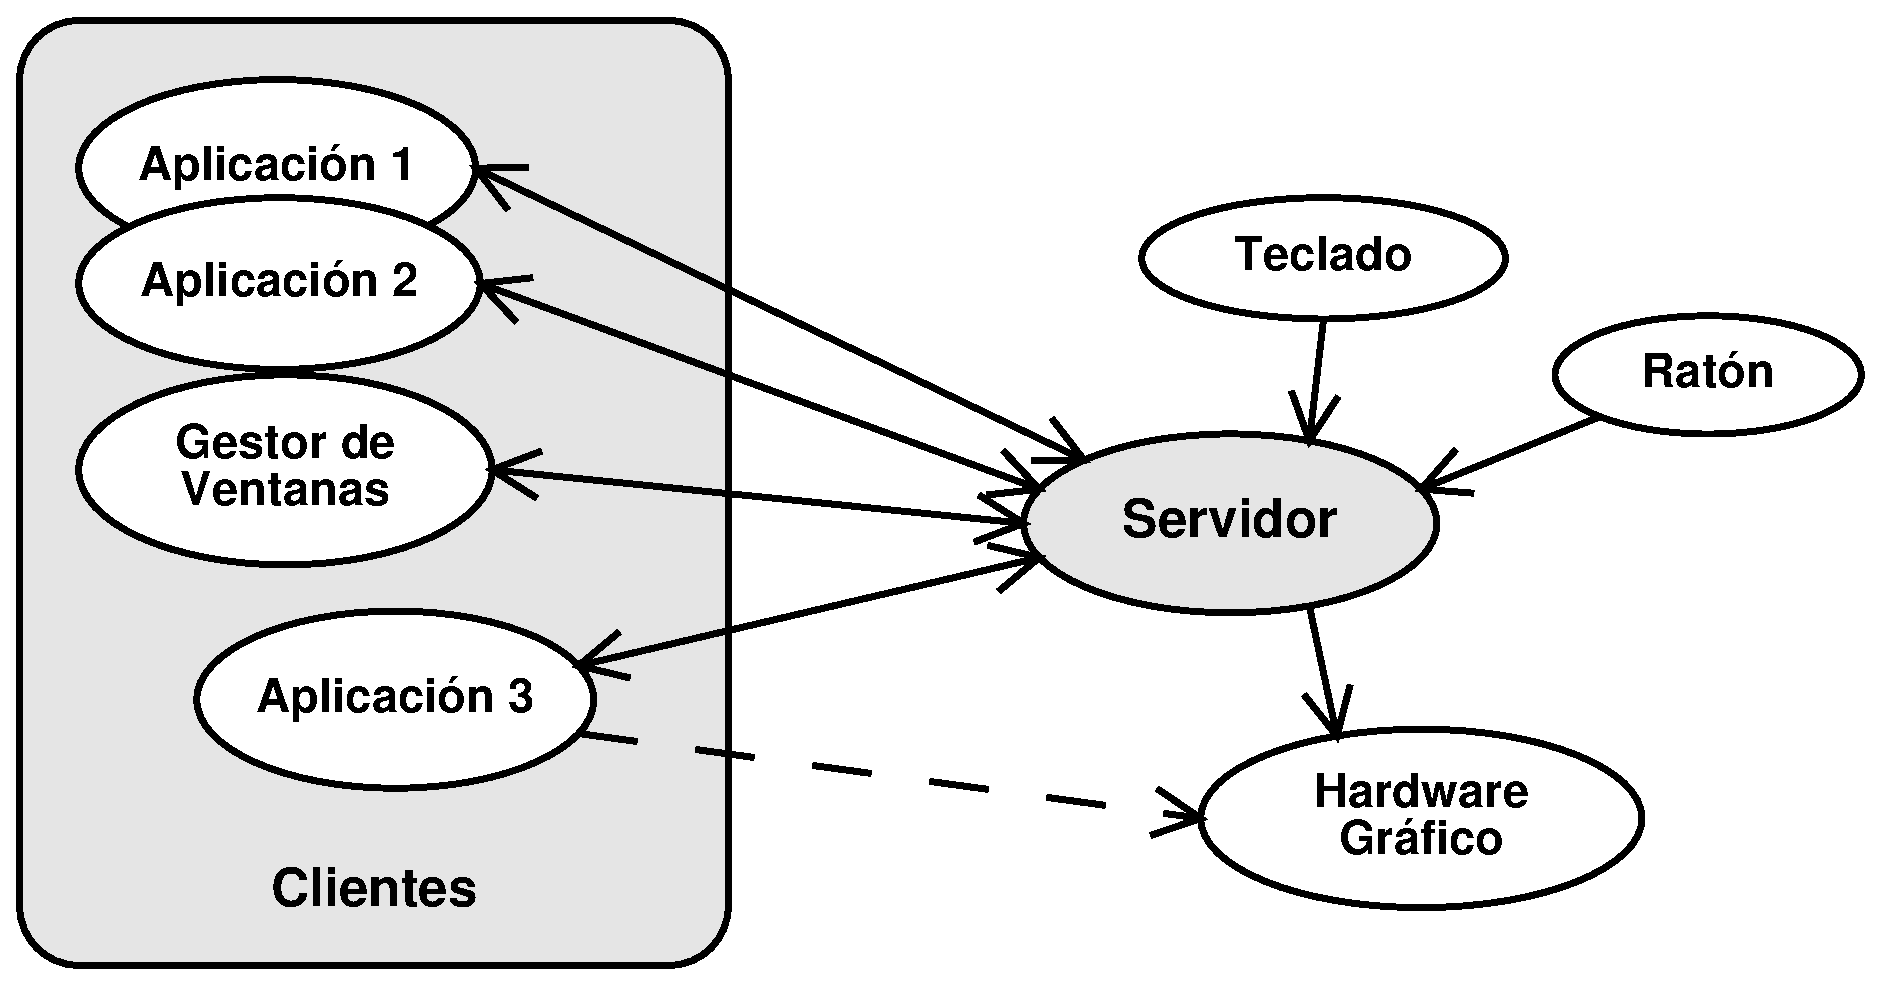
\includegraphics[width=0.95\textwidth]{imagenes/xwindow.eps}
\caption{Arquitectura cliente/servidor del sistema X-Window}\label{xwindow}
\end{figure}

La arquitectura de las X se divide en dos elementos fundamentales. Por
un lado el  {\em servidor X}\index{servidor X}  encargado de gestionar
el  uso de  los dispositivos  de  salida (p.ej.  tarjetas gr�ficas)  y
de  los dispositivos  de  entrada (p.ej.  teclados, ratones,  tabletas
digitalizadoras, etc). Por el  otro los {\em clientes X}\index{cliente
X} nombre  con el  que se conoce  a cada una  de las  aplicaciones que
hacen uso del  sistema X. Las pulsaciones de tecla,  el movimiento del
rat�n  o cualquier  otra acci�n  del  usuario en  los dispositivos  de
entrada es detectada por servidor y  transferida a los clientes. De la
misma manera  los clientes transfieren  al servidor las  peticiones de
operaciones a realizar sobre el dispositivo de salida (p.ej. trazar un
l�nea  en pantalla,  dibujar  un  punto, volcar  un  bitmap, etc).  La
comunicaci�n entre cliente y servidor sigue un protocolo estandarizado
que corre sobre los servicios de red del sistema. Esto permite que los
clientes no tengan porqu� estar en la misma m�quina que el servidor. O
sea que podemos tener un servidor  X en nuestra m�quina local a trav�s
del que  interactuar con clientes que  se ejecutan de forma  remota en
otro ordenador,sin que  por ello notemos diferencia  alguna. Aparte de
todo esto  las X realizan ciertas  optimizaciones en los casos  en los
que cliente y servidor se encuentran  en la misma m�quina. Por ejemplo
se  permite  el acceso  directo  al  hardware  de v�deo  ignorando  el
protocolo descrito,  con lo que  se aprovechan las  caracter�sticas de
aceleraci�n  3D  de  muchas  tarjetas  modernas. Con  ello  las  X  se
convierten  en  una  plataforma  potente  para  ejecutar  aplicaciones
exigentes  desde un  punto de  vista gr�fico  sin por  ello perder  su
flexibilidad.

Otra caracter�stica  interesante del  sistema X  es que  podemos tener
varios servidores  en una  misma m�quina,  donde cada  uno es  un {\em
ente} independiente que utiliza sus  propios dispositivos de entrada y
salida. Evidentemente no es habitual disponer de m�s de un monitor y/o
teclado pero  en ocaciones  se pueden  utilizar servidores  sin salida
gr�fica. Tambi�n es  posible que todos usen los  mismos dispositivos y
que se habilite alg�n mecanismo  para que podamos conmutar entre ellos
a voluntad.


\subsection{Gestores de ventanas}

En  todo  buen  entorno  gr�fico  moderno  las  aplicaciones  utilizan
ventanas para  interactuar con el  usuario. Sin embargo el  servidor X
s�lo entiende un n�mero limitado  de primitivas gr�ficas, como dibujar
l�neas  y puntos  o copiar  �reas  de la  pantalla. Por  ello se  hace
necesaria la presencia de una aplicaci�n cliente {\em especial} que se
encargue de  crear, destruir,  mover, gestionar el  foco y  en general
gestionar  todas las  cuestiones referentes  al comportamiento  de las
ventanas, utilizando para ello las  primitivas del servidor X. A dicha
aplicaci�n  se la  denomina {\em  gestor de  ventanas}\index{gestor de
ventanas}. En la Figura \ref{xwindow}  podemos ver su situaci�n dentro
de la arquitectura de las X-Window.

En una  distribuci�n de  Linux pueden  haber cerca  de 40  gestores de
ventanas  entre los  que un  usuario debe  elegir. Cada  uno de  ellos
imprime  un {\em  feeling}  diferente a  nuestro  entorno de  trabajo.
Tengamos en cuenta  que cada gestor dibuja los elementos  del marco de
nuestras ventanas  de forma  diferente (e.j. la  barra de  t�tulo, los
botones  de  control, los  bordes),  dot�ndolos  de un  comportamiento
particular  y  caracter�stico seg�n  las  preferencias  del equipo  de
programadores  que  lo dise��.  Empezando  por  los est�ticamente  m�s
valorados como {\em Windows Maker}  o {\em Enlightenment}; pasando por
los  que imitan  a  otros sistemas  como {\em  AfteStep}  o {\em  F(?)
Virtual Window  Manager} (en una  de sus variantes nos  proporciona el
look de Microsoft� Windows� 95); o los que permiten ser personalizados
con  {\em temas}  diferentes como  {\em  Ice Windows  Manager} o  {\em
Sawfish}; y  terminando por los  m�s ligeros  y r�pidos pero  no menos
funcionales como  {\em Fast  Light Window Manager}  se cubre  toda una
variedad de necesidades del usuario.


\subsection{Entornos de escritorio}

Ahora que  disponemos de  ventanas se  hace necesario  rellenarlas con
algo.  A la  hora de  programar  una aplicaci�n  para las  X se  suele
recurrir a  los {\em toolkits}\index{toolkits}. Se  trata de librer�as
dise�adas  para proporcionar  diferentes  tipos de  controles (p.  ej.
botones,  barras de  men�s, cuadros  de edici�n,  etc) facilitando  su
gesti�n. Las toolkits  crean los controles all� d�nde  le digamos, los
destruyen,  los  redibujan  cuando  es necesario,  manejan  todas  las
acciones que se  hagan sobre ellos a  trav�s del uso de  alguno de los
dispositivos de entrada  posibles, etc. Trabajar sin hacer  uso de los
toolkits implicar�a dise�ar y gestionar nuestros propios controles.

Es importante destacar  que una aplicaci�n X funciona sea  cual sea el
gestor de  ventanas seleccionado. Por tanto,  el uso de uno  u otro es
una elecci�n personal del usuario. Sin embargo, el uso de un toolkit u
otro en una aplicaci�n es elecci�n  del equipo de programadores que ha
trabajado en ella. Eso unido a  la gran variedad de toolkits existente
en  Linux convierte  nuestro  escritorio en  una  selva donde  podemos
ver  una fauna  de  aplicaciones  con interfaces  gr�ficas  de lo  m�s
variopinto.

Para garantizar  que las aplicaciones presenten  una interfaz similar,
reduciendo la curva de aprendizaje  de los usuarios, han aparecido los
{\em entornos de  escritorio}. B�sicamente se trata  de establecer una
serie de  reglas comunes  que suelen incluir:  el toolkit  a utilizar,
el  formato  de la  ayuda,  el  modelo  de componentes,  librer�as  de
tratamiento de  im�genes y sonido, etc.  Todo ello genera un  marco de
trabajo  tanto  para los  desarrolladores  de  nuevas como  de  viejas
aplicaciones.  Si  los  desarrolladores  se ci�en  a  dicho  marco  el
resultado es un entorno de trabajo  uniforme y c�modo donde no existen
diferencias sustanciales en la interfaz de una aplicaci�n a otra.

Afortunadamente  la variedad  es una  caracter�stica de  Linux. En  la
actualidad disponemos de dos grandes entornos de escritorio:

\begin{description}

\item[GNOME]\index{GNOME} Funciona  con el toolkit  GTK\index{GTK} que
fue originalmente dise�ado para  GIMP. Quiz�s las principales ventajas
de este entorno  no est�n tanto del  lado del usuario como  del de los
programadores, de la tecnolog�a que subyace debajo del sistema y de la
declaraci�n de intenciones con la que se inici� el proyecto.

\item[KDE]\index{KDE} Funciona sobre el  toolkit Qt\index{Qt}, lo cual
provoc�  una gran  pol�mica  en sus  or�genes al  no  disponer de  una
licencia todo  los {\em libre} que  se deseaba. En la  actualidad esos
problemas se  han resuelto y es,  hoy por hoy, considerado  por muchos
como el entorno con la interfaz m�s atractiva de los dos.

\end{description}

Cada  uno tiene  sus m�s  y sus  menos pero  la gran  realidad es  que
presentan una interfaz muy intuitiva que se aprende a manejar desde el
primer momento.


\section{Primer contacto con las X con GNOME}

Debido a la sencillez de los  entornos de escritorio resulta absurdo e
in�til  intentar explicar  detalladamente  su manejo.  La mejor  forma
de  aprender  es sentarnos  delante  de  uno  de  ellos, ser  un  poco
osado  y ante  todo tener  la  buena costumbre  de leer  detenidamente
todo  aquello que  nos indique  el sistema.  Sin embargo,  si vamos  a
realizar una  primera toma de  contacto guiada en la  que aprenderemos
algunos conceptos  b�sicos que nos ser�n  de gran ayuda en  el futuro.
Las  limitaciones  de  tiempo  nos  obligan a  centrarnos  en  uno  de
los  dos  entornos de  escritorio.  En  nuestro caso  nos  centraremos
en  GNOME\index{GNOME}.  Sin embargo,  los  devotos  de KDE  no  deben
preocuparse puesto que conociendo  uno resulta extremadamente sencillo
llegar a dominar el otro.

Al iniciar  un sistema Linux con  las X instaladas es  probable que se
nos permita autentificarnos  desde el modo gr�fico.  En caso contrario
s�lo  dispondremos  de  una  consola  esperando  a  que  introduzcamos
el  nombre  de  usuario.  Si  nuestro  caso  es  este  �ltimo  debemos
autentificarnos, y ejecutar el comando  {\tt startx} cuando el sistema
nos indique  que est�  disponible para  recibir nuestros  comandos. El
comando  {\tt startx}  iniciar� el  entorno gr�fico.  Evidentemente al
terminar nuestro trabajo volveremos a la consola.

\begin{figure}[hbtp]
\centering
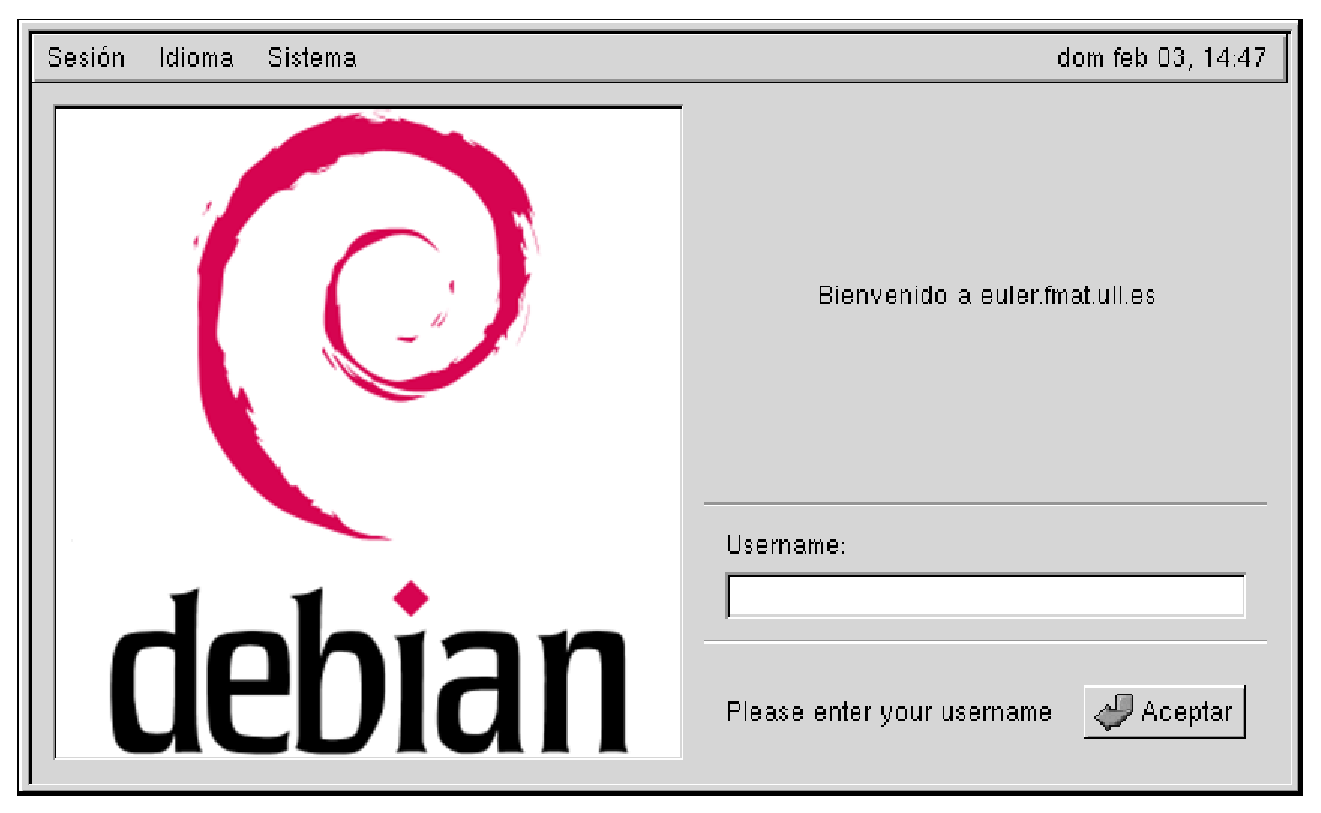
\includegraphics[width=0.95\textwidth]{imagenes/gdm.eps}
\caption{Ventana de autentificaci�n de GDM}\label{gdm}
\end{figure}

Para  que la  autentificaci�n desde  el  modo gr�fico  sea posible  es
necesario  tener  instalado  un  {\em  display  manager}.  Algunos  de
ellos  son  {\tt  xdm}\index{xdm}, {\tt  kdm}\index{kdm}  (KDE),  {\tt
gdm}\index{gdm}  (GNOME), etc.  Como ya  hemos comentado  nosotros nos
centraremos  en GNOME,  y  por  tanto en  este  �ltimo.  En la  Figura
\ref{gdm} podemos ver un ejemplo de la cl�sica ventana que nos muestra
GDM  nada m�s  terminar la  carga  del sistema.  B�sicamente nos  est�
pidiendo nuestro nombre  de usuario, para una vez  pulsado {\tt enter}
pedirnos la password. Con esa informaci�n seremos autentificados en el
sistema y se iniciar� una nueva  sesi�n con nuestra cuenta de usuario.
Es  importante destacar  que  dentro  de nuestra  sesi�n  todo lo  que
hagamos es personal.  Eso quiere decir que los cambios,  sean del tipo
que sean, s�lo  afectar�n a nuestra sesiones futuras pero  no a las de
los otros usuarios de la m�quina.

Volviendo al  GDM, este  dispone de  algunas opciones  adicionales que
podemos emplear antes de iniciar el proceso de autentificaci�n.

\begin{description}

\item[SESI�N] Nos permite elegir la  naturaleza de la pr�xima sesi�n a
iniciar. Opciones habituales son GNOME y KDE. Elegi�ndolas iniciaremos
sesi�n  con el  entorno de  escritorio que  prefiramos. Tambi�n  puede
haber alguna sesi�n  especial {\em a prueba de fallos},  o que carezca
de  un entorno  de escritorio  espec�fico,  o cualquier  otro tipo  de
sesi�n  que el  administrador del  sistema halla  deseado incluir.  La
opci�n por defecto es {\tt �LTIMA} que hace referencia a entrar con el
tipo de  sesi�n que  tenemos asignado nosotros  por defecto.  Si nunca
hemos elegido ninguno lo normal es  que el tipo por defecto sea GNOME.
Si hacemos una selecci�n diferente a  la opci�n por defecto el sistema
nos preguntara  si queremos que  el nuevo  tipo de sesi�n  sea nuestra
sesi�n por defecto,  y por tanto a la que  que corresponder� la opci�n
{\tt �LTIMA} la pr�xima vez.

\item[IDIOMA] Aparte  de elegir  sesi�n podemos seleccionar  el idioma
con el  que queremos  trabajar. Las aplicaciones  traducidas mostrar�n
toda la informaci�n  en dicho idioma. Igual que antes,  la opci�n {\tt
�LTIMA}  habla de  nuestra �ltima  selecci�n, es  decir el  idioma por
defecto.

\item[SISTEMA] Nos permite apagar, suspender o reniciar la maquina. En
algunos sistemas, y siempre y cuando dispongamos de la cuenta del {\tt
root},  nos permite  configurar  GDM. Es  importante  recordar que  al
cerrar  nuestra sesi�n  volvemos a  la ventana  de GDM  por lo  que si
deseamos apagar  el sistema  �ste ser�a el  momento de  seleccionar la
opci�n correspondiente.

\end{description}

Antes  de continuar  es importante  destacar algunas  cosas. En  Linux
existe lo que se  denomina {\em terminales virtuales}\index{terminal}.
Si estamos  en modo texto podemos  usar la combinaci�n de  teclas {\tt
Alt+F?} para pasar de un terminal  a otro. Eso se comprueba f�cilmente
porque vemos  c�mo cambia el contenido  de la pantalla. El  uso de los
terminales virtuales  nos permite mantener varias  sesiones abiertas y
trabajar de forma independiente en ellas. Cuando se inicia un servidor
X  �ste queda  asociado a  uno de  esos terminales  virtuales (podemos
tener varios servidores asociados a distintos terminales); normalmente
al  {\tt  F7}.  Debido al  mecanismo  por  el  que  las X  manejan  el
teclado, en  los terminales asociados  a servidores  X ya no  se puede
usar  {\tt Alt+F?}  sino que  para  cambiar de  terminal debemos  usar
{\tt  Ctrl+Alt+F?}. Usando  la primera  combinaci�n de  teclas en  los
terminales en  modo texto  y la  �ltima en  los asociados  a las  X no
tendremos problemas para movernos por ellos  y pasar de modo gr�fico a
consola a nuestro antojo.

Otro punto  importante es que s�lo  cuando veamos un mensaje  del tipo
{\tt Kernel Panic}  podemos decir que nuestro Linux se  ha colgado. En
cualquier  otro  caso  estamos  frente a  sencillos  cuelgues  de  las
aplicaciones con  las que  trabajamos. No debemos  preocuparnos puesto
que Linux proporciona  los suficientes recursos como  para que podamos
recuperar el control  de la m�quina. Por ejemplo podemos  cambiar a un
terminal diferente  de la consola  para matar aplicaciones que  se han
quedado  colgadas en  nuestro  terminal  de trabajo  o  en  las X.  En
situaciones cr�ticas puede  ser necesario terminar con las  X de forma
prematura. Para  ello se  pulsa la secuencia  {\tt Ctrl+Alt+Backspace}
que cierra  el servidor X  abortando todas las  aplicaciones gr�ficas.
Evidentemente los datos no guardados se perder�n.

\begin{figure}[hbtp]
\centering
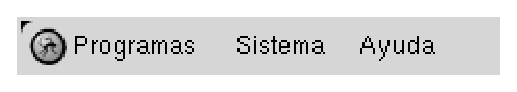
\includegraphics{imagenes/menu.eps}
\caption{Men� de panel de GNOME}\label{menu}
\end{figure}

\begin{figure}[hbtp]
\centering
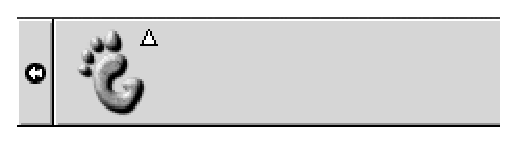
\includegraphics{imagenes/panel.eps}
\caption{Panel de alineado de GNOME}\label{panel}
\end{figure}

Suponiendo  que iniciamos  sesi�n en  la  m�quina lo  primero que  nos
llamar�  la  antenci�n  son  los  {\em  paneles}  (Figuras  \ref{menu}
y  \ref{panel}).  Si pulsamos  en  la  huella  del panel  inferior,  o
seleccionamos alguna de las  opciones del panel superior, dispondremos
de acceso a las aplicaciones instaladas  en el sistema. La mayor parte
de las aplicaciones  GNOME est�n clasificadas y  disponibles en alguno
de  los submen�s  correspondientes. (p.  ej. {\tt  APLICACIONES}, {\tt
UTILER�AS}, {\tt  GR�FICOS}, etc).  En {\tt  MEN�S KDE}  se encuentran
clasificadas todas  las aplicaciones KDE  instaladas, y en  {\tt MEN�S
DEBIAN} todas  las aplicaciones de la  distribuci�n independientemente
del entorno de  escritorio para las que fueron  desarrolladas. En este
punto es  importante recordar que  podemos ejecutar cualquiera  de las
aplicaciones  sin importar  que estemos  trabajando en  un entorno  de
escritorio diferente a aquel para el que fueron dise�adas.

Otras  opciones son  el men�  {\tt FAVORITOS},  que es  personalizable
con  nuestras  aplicaciones preferidas,  la  opci�n  {\tt BLOQUEAR  LA
PANTALLA}, para proteger nuestro escritorio si tenemos que abandonarlo
por  cualquier  motivo  (es  importante recordar  que  de  esa  manera
evitaremos  que  manipulen  nuestros   datos  pero  siempre  queda  la
posibilidad  de  que  pulsen  {\tt  Ctrl+Alt+Backspace}  para  abortar
todas las  aplicaciones gr�ficas, perdiendo  los datos no  guardados y
volviendo a  la ventana de inicio  de sesi�n del GDM),  la opci�n {\tt
TERMINAR SESI�N} para terminar nuestra  sesi�n y volver al GDM (Figura
\ref{gdm}). Si accedemos a  {\tt CONFIGURACI�N $\rightarrow$ CENTRO DE
CONTROL DE GNOME} dispondremos de todas las opciones para personalizar
nuestro escritorio.

Manejar GNOME  es cuesti�n de  jugar un  rato y probar  las diferentes
opciones. Disponemos de  tres botones en nuestro  rat�n (ya hablaremos
de eso m�s adelante) y se trata de utilizarlos sobre los elementos del
escritorio para  ver como reaccionan.  Por ejemplo sobre los  iconos o
sobre el  fondo del escritorio, sobre  los men�s, sobre la  huella del
panel inferior,  sobre una parte descubierta  de un panel o  sobre las
peque�as aplicaciones que se ejecutan sobre ellas. Por cierto que esas
peque�as  aplicacions  se  denominan  {\em  applets}\index{applets}  y
podemos  instalar cuantas  queramos si  jugamos un  poco con  el bot�n
derecho  de  nuestro  rat�n  y  una  parte  descubierta  de  un  panel
cualquiera. Otros ejemplos se consiguen al pulsar con el bot�n derecho
sobre un men� y as� poder  elegir a�adirlo a {\tt FAVORITOS}, o pulsar
sobre la l�nea discontinua de la  parte superior de los men�s para ver
como se despendren y quedan en una ventana a parte.

En Linux existen muchos {\em emuladores de terminal}. Dichos programas
permiten ejecutar aplicaciones  de modo consola dentro  de una ventana
X.  El m�s  b�sico es  el {\tt  xterm}\index{xterm} que  viene con  la
instalaci�n  est�ndar de  las  X,  pero existen  muchos  otros y  cada
entorno suele venir  con uno propio. El de GNOME  est� en {\tt SISTEMA
$\rightarrow$ TERMINAL  UNIX DE  GNOME}. En  ocasiones es  posible que
intentemos  ejecutar  una aplicaci�n  que  nunca  llega a  mostrar  su
ventana principal o que da alg�n tipo de error grave. En esos casos es
recomendable ejecutar el programa desde  el emulador de terminal. Como
ya hemos comentado las aplicaciones para  X no son diferentes de otras
aplicaciones por lo que suelen  mostrar informaci�n por la consola, si
esta est�  disponible. Esa informaci�n  puede ser vital  para resolver
nuestro problema.

Cuando ejecutamos una  aplicaci�n X desde el emulador  de terminal (p.
ej. {\tt gnome-edit}  que es el editor por defecto  del entorno GNOME)
vemos que  �ste se queda  bloqueado a la  espera de que  la aplicaci�n
termine. Esto no  deber�a sorprendernos puesto que  en realidad ocurre
lo mismo cuando ejecutamos una aplicaci�n  de consola. Para que eso no
suceda  debemos  a�adir  un  {\tt  \&} al  final  del  comando  de  la
aplicaci�n  X,  o pulsar  {\tt  Ctrl+Z}  y  ejecutar el  comando  {\tt
bg}\index{bg} sobre el emulador despu�s de que la aplicaci�n haya sido
iniciada. De esta manera la aplicaci�n  X pasa a ejecutarse en segundo
plano, liberando al emulador de terminal para que pueda recibir nuevos
comandos.

En  general mostrar  el  cl�sico  aviso de  que  una aplicaci�n  tiene
archivos  modificados y  va a  ser  cerrada es  responsabilidad de  la
propia aplicaci�n. El cierre de  la ventana principal por la pulsaci�n
del  correspondiente bot�n  en la  barra  de t�tulo  es notificado  al
proceso propietario de la ventana.  Normalmente se suele mostrar dicho
mensaje y  una vez  aceptado se  termina el proceso.  Por una  lado es
posible que nuestra aplicaci�n no  disponga de esa caracter�stica. Por
ejemplo si cerramos el emulador  de terminal cuando estamos ejecutando
sobre  �l  cualquier tipo  de  aplicaci�n  (sea  de  consola o  de  X)
dicha aplicaci�n  termina inmediatamente perdi�ndose los  datos que no
hubieran  sido  guardados.  O  sea,  como  en  el  caso  anterior,  si
ejecutamos {\tt gnome-editor} sobre el terminal, escribimos algo sobre
el editor, y  cerramos el terminal, veremos como  nuestra apliaci�n de
edici�n  terminar� sin  advertir nada  de la  p�rdida de  datos, y  el
terminal se cerrar�  sin indicarnos que se encuentra  esperando por el
editor.

\begin{figure}[hbtp]
\centering
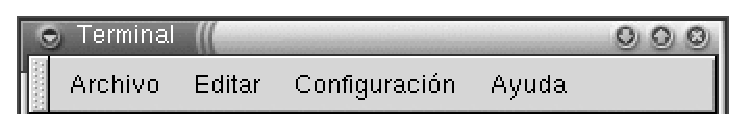
\includegraphics{imagenes/btitulo.eps}
\caption{Barra de t�tulo del gestor de ventanas Sawfish}\label{btitulo}
\end{figure}

Por otro  lado es posible  que el proceso  est� bloqueado y  no reciba
el  mensaje.  En  ese caso  la  ventana  no  se  cerrar� a  menos  que
forcemos su destrucci�n  con la opci�n correspondiente en  el men� del
marco  de  la  venta  (Figura  \ref{btitulo}, men�  del  bot�n  de  la
izquierda).  Entonces  el  gestor  de  ventanas  la  cerrar�  pero  la
aplicaci�n seguir� ejecut�ndose en  segundo plano aunque para nosotros
ya no  exista. La �nica  soluci�n ser� matarla  a mano con  el comando
{\tt  kill}\index{kill} desde  un emulador  de terminal.  Si vemos  un
consumo de CPU  excesivo o un sistema demasiado lento  puede deberse a
la existencia de procesos en segundo plano que no fueron destruidos en
su momento. Una aplicaci�n interesante es {\tt xkill}\index{xkill}. Si
la ejecutamos nos  aparecer� un punto de mira en  el cursor de nuestro
rat�n.  Al  pulsar sobre  una  ventana  la  aplicaci�n se  encarga  de
destruir al proceso asociado a la misma.

Como hemos dicho anteriormente, a la hora  de aprender a usar las X no
basta con jugar con los botones  izquierdo y derecho de nuestro rat�n.
En las X  el bot�n central es de tanta  importancia que suele disponer
de funciones adicionales  que no est�n presentes en los  otros dos. En
entornos de escritorio como KDE o GNOME esto suele implicar un men� de
contexto adicional al que se muestra  usando el bot�n derecho; pero en
otras  aplicaciones  podemos encontrar  formas  de  manejo de  lo  m�s
curiosas. Tal es  su importancia que en  caso de no disponer  de �l se
emula  por la  pulsaci�n simultanea  de los  dos botones  est�ndar del
rat�n. Una  aplicaci�n interesante  del bot�n central  es su  uso para
copiar texto entre  aplicaciones sea cual sea la toolkit  bajo las que
hayan  sido  desarrolladas.  Basta  con marcar  nuestro  texto  en  la
aplicaci�n de  origen para  que al  pulsar el bot�n  central en  la de
destino �ste se pegue a continuaci�n de la posici�n actual del cursor.
En el servidor X  existe un b�ffer que se llena  cada vez que marcamos
texto en  alguna aplicaci�n. El bot�n  central del rat�n lo  �nico que
hace  es volcar  ese  texto  como si  hubiera  sido  escrito desde  el
teclado. Por  tanto para  utilizar este sistema  es importante  ser lo
suficientemente cuidadoso  como para  no marcar  otra cosa  despu�s de
marcar el texto a copiar.


\section{Primer contacto con las X con KDE}

% Aqu� le toca escribir a MojoPiKon y A-r-C

%Autor: aplatanad, amd77, faraox

\chapter{Aplicaciones para Internet}

\section{Navegadores web}

\subsection{Netscape Communicator 4 }
      

Durante   algunos  a�os,   Netscape   ha  sido   el  �nico   navegador
multiplataforma real, dando  cobertura a muchos de  los distintos Unix
comerciales existentes.  Casi desde que Linux  tiene interfaz gr�fico,
ha  existido una  versi�n  del navegador  Netscape  para este  sistema
operativo.


{\sf Netscape  Communicator 4} proporciona soporte  para navegaci�n de
p�ginas web  con JavaScript y  Flash 5, permite  visualizar documentos
PDF  dentro del  navegador  (mediante  un plugin  para  el {\sf  Adobe
Acrobat Reader}). Tambi�n nos  permite gestionar el correo electr�nico
y componer p�ginas web.

Los  Linuxeros siempre  hemos  considerado que  el navegador  Netscape
consum�a  demasiados  recursos en  Linux,  adem�s  de tener  bastantes
problemas  de  estabilidad.   Debido  a  �ste,  y   a  otros  factores
importantes, como fueron  la forma de competir con  la casa Microsoft,
Netscape lleg� a la sana conclusi�n de que la mejor manera de mantener
su navegador en el mercado, era  liberando su c�digo fuente. As� naci�
{\sf Mozilla}.

Como debe ser,  dentro de la comunidad del Software  Libre, se alzaron
voces  en  contra  de  ese desperdicio  de  recursos,  proponiendo  la
creaci�n  de navegadores  alternativos. Aqu�  listamos algunas  de las
alternativas que podemos  encontrar en el �rea de  los navegadores web
dentro del Software Libre:

\begin{itemize}
\item{\sf chimera2} - Navegador web para las X
\item{\sf communicator} - Netscape Communicator 4.77
\item{\sf dillo} - Navegador web basado en las GTK
\item{\sf encompass} - Un navegador libre para GNOME
\item{\sf galeon} - Navegador basado en Mozilla, con el aspecto y la apariencia de las aplicaciones GNOME
\item{\sf konqueror} - El gestor de ficheros, navegador web y visor de documentos del KDE
\item{\sf links} - Navegador web en modo c�racter
\item{\sf lynx} - Navegador web en modo c�racter
\item{\sf mozilla} - Un navegador Open Source para las X's. Es el heredero de Netscape.
\item{\sf OpenOffice} - Suite ofim�tica que incluye un buen navegador web
\item{\sf w3m} - Visor web con un excelente soporte para tablas y marcos
\end{itemize}

Bueno, seguro que en el momento  de leer este apartado, habr�n surgido
nuevos navegadores web dentro del mundillo del Software Libre



\section{Transferencia de ficheros (FTP)}


FTP  (File Transfer  Protocol) es  un  protocolo que  se utiliza  para
transferir informaci�n, almacenada en  ficheros, de una m�quina remota
a  otra local,  o viceversa.  Para  poder realizar  esta operaci�n  es
necesario conocer la direcci�n  IP o el nombre de la  m�quina a la que
nos queremos  conectar para realizar  alg�n tipo de  transferencia. Es
fundamental distinguir entre m�quina local y m�quina remota:

\begin{description}

\item[M�quina local] Es aqu�lla desde  donde nos conectamos para hacer
la transferencia, es decir, donde ejecutamos ftp.

\item[M�quina  remota]  Es  aquella  a  la  que  nos  conectamos  para
transferir informaci�n.

\end{description}

\subsection{ Inicio de sesi�n FTP}

Para  realizar  transferencias  de   ficheros  por  protocolo  FTP  se
establecen conexiones (sesiones)  entre la m�quina local  y la remota.
Estas  sesiones  comienzan  por   la  autentificaci�n  del  usuario  y
prosiguen  con las  transferencias.  Finalmente la  sesi�n se  cierra.
Veamos un ejemplo:

\begin{verbatim}
$ ftp euler
Connected to euler.fmat.ull.es.
220 ProFTPD 1.2.0pre10 Server (Debian) [euler.fmat.ull.es]
Name (euler:miguev): 
\end{verbatim}

El servidor  nos preguntar�  un nombre de  usuario, y  seguidamente la
contrase�a.  El nombre  que daremos  debe  ser una  cuenta de  usuario
v�lida  en el  servidor al  que  intentamos acceder,  y la  contrase�a
l�gicamente  debe ser  correspondiente  a ese  usuario. En  servidores
p�blicos suele existir una cuenta de  acceso an�nima s�lo para leer (o
tal vez una carpeta donde poner cosas pero no leer). Para acceder a un
FTP como  usuario an�nimo se  utiliza el  nombre {\tt anonymous}  y se
proporciona la direcci�n de correo electr�nico como contrase�a.

Una vez introducido el nombre y la contrase�a el servidor nos recibir�
y el programa cliente de FTP  nos mostrar� un prompt, manifestando as�
que est� preparado para ejecutar las �rdenes que le demos. A partir de
aqu� se realizan  las maniobras posibles mediante los  com�ndos de FTP
que veremos m�s adelante.

\begin{verbatim}
$ ftp euler
Connected to euler.fmat.ull.es.
220 ProFTPD 1.2.0pre10 Server (Debian) [euler.fmat.ull.es]
Name (euler:miguev): miguev
331 Password required for miguev.
Password:
230 User miguev logged in.
Remote system type is UNIX.
Using binary mode to transfer files.
ftz>
\end{verbatim}



\subsection{Comandos del FTP}


El protocolo FTP dispone de unos comandos est�ndares suficientes 
para las operaciones de transferencia de ficheros, de los cuales
vemos a continuaci�n un resumen.


\begin{description}

\item[help]  Proporciona una  lista  de  los comandos  del  FTP de  la
m�quina local

\item[help   comando]  Proporciona   informaci�n   sobre  el   comando
especificado, correspondeinte a la m�quina local

\item[lcd directorio-local] Para moverse de un directorio a otro en la
m�quina local

\item[lcd unidad:] Para  cambiar de una unidad de disco  a otra, en el
caso particular de que la m�quina local esa un PC con Windows o MS-DOS

\item[cd directorio-remoto] Para moverse de un directorio a otro en la
m�quina remota

\item[lls directorio-local] Para listar  el contenido de un directorio
en la m�quina local

\item[[ls|dir]  directorio-remoto]  Para  listar el  contenido  de  un
directorio en la m�quina remota

\item[! comando] Para ejecutar un comando en la m�quina local

\item[delete  fichero-remoto] Para  borrar  un fichero  en la  m�quina
remota

\item[delete  ficheros-remotos]  Para  borrar varios  ficheros  en  la
m�quina remota

\item[rmdir directorio-remoto] Para borrar un directorio en la m�quina
remota

\item[mkdir directorio-remoto] Para crear  un directorio en la m�quina
remota

\item[pwd] Para saber  el directorio en el que se  est�, en la m�quina
remota

\item[ascii] Para hacer la transferencia en formato ASCII (lo hace por
defecto)

\item[binary]  Para  hacer la  transferencia  en  formato binario,  se
utiliza el comando:

\item[get   fichero-remoto    fichero-local]   Transfiere    el   {\tt
fichero-remoto}  desde   la  m�quina   remota  a  la   m�quina  local,
guard�ndolo con el nombre {\tt fichero-local} en la m�quina local

\item[mget  lista-ficheros-remotos] Transfiere  los ficheros  listados
desde la m�quina remota a la m�quina local.

\item[prompt] (Des)activa el modo interactivo de las transferencias de
ficheros m�ltiples.

\item[put   fichero-local    fichero-remoto]   Transfiere    el   {\tt
fichero-local} desde la m�quina local a la m�quina remota, guard�ndolo
con el nombre {\tt fichero-remoto} en la m�quina remota

\item[mput  lista-ficheros-locales] Transfiere  los ficheros  listados
desde la m�quina local a la m�quina remota.

\end{description}

Obviamente, el  comando {\tt ftp} no  es el �nico programa  cliente de
FTP disponible. Existen  multitud de programas clientes  de FTP, tanto
para GNU/Linux como para otras plataformas, como p.ej. el gFTP.



\section{Acceso remoto (SSH)}


En muchas ocaciones resulta interesante acceder a una m�quina remota y
trabajar como  si estuvi�ramos  f�sicamente frente  a ella.  Es decir,
hablamos de  poder ejecutar  comandos en dicha  m�quina sin  tener que
trasladarnos  a escribirlos  en  su teclado.  Este  tipo de  servicios
existe desde  los or�genes de  Internet pero siempre ha  entra�ado sus
riesgos dado que  es necesaria la autentificaci�n  remota del usuario.
Para entender  de lo  que estamos  hablando s�lo  es necesario que nos
aproximemos  al servicio  de {\tt  TELNET} (cuyo  cliente suele  estar
disponible bajo el comando del mismo nombre).

TELNET\index{TELNET} fue el primer  servicio de acceso remoto dise�ado
para  Internet.  B�sicamente el  comando  {\tt  telnet} toma  nuestras
pulsaciones de  teclado y las trasnmite  por la red hasta  el servidor
TELNET de la m�quina remota a  la que estamos conectados. �ste toma la
salida  a terminal  de la  aplicaciones que  vayamos ejecutando  y las
env�a  a  nuestro cliente  en  la  m�quina  local. Ese  mecanismo  tan
sencillo  resuelve  el problema  del  acceso  remoto; excepto  por  un
peque�o  problema. Toda  la comunicaci�n  se realiza  en texto  plano.
Es  decir,  el texto  se  env�a  tal  cual,  sin mecanismo  alguno  de
compresi�n  y/o encriptaci�n  que altere  las cadenas  de texto.  Todo
lo  que  escribimos (p.ej.  comandos  del  int�rprete de  comandos)  y
recibimos (p.ej. correo, informes, cartas) puede ser visto por quienes
intercepten nuestros  paquetes. Esto es especialmente  cr�tico durante
el  proceso de  conexi�n, momento  en  el que  debemos enviar  nuestro
nombre de usuario y contrase�a para realizar la autentificaci�n remota
a la que aludimos anteriormente. Es  evidente que en esa etapa nuestra
password, y  con ella  el acceso  al servidor  bajo nuestro  nombre de
usuario, queda al descubierto.

A   efectos  pr�cticos   la   mayor  parte   de   los  protocolos   de
Internet  se  fundamentan en  TELNET.  Servicios  como la  World  Wide
Web  (HTTP\index{HTTP}),  el   correo  electr�nico  (SMTP\index{SMTP},
POP\index{POP},  IMAP\index{IMAP}),  las  transferencias  de  ficheros
(FTP\index{FTP}), la administraci�n de la red (SMNP\index{SMNP}), etc.
utilizan  protocolos  cuyas  especificaciones  indican  claramente  su
v�nculo con TELNET. Si ya resulta  grave que en todas esas situaciones
nuestros datos queden al descubierto, m�s lo es aun cuando hablamos de
permitir o  denegar el  acceso a  un servicio tan  cr�tico como  es el
acceso remoto. �ste suele poner las  cosas m�s faciles que ning�n otro
para quien desee atacar el sistema.

Dos son las cosas que debemos recordar de todo lo anterior:

\begin{itemize}

\item {\bf  En condiciones normales  la mayor  parte de los  datos que
enviamos y/o  recibimos de Internet  est�n al descubierto.}  Es decir,
una  vez interceptados  pueden  ser le�dos  directamente sin  requerir
ning�n proceso intermedio.

\item  {\bf  No debemos  utilizar  TELNET  bajo ning�n  concepto.}  El
comando {\tt telnet} puede ser una herramienta muy pr�ctica en algunos
casos, pero peligrosa si la usamos para acceso remoto.

\end{itemize}

La  cuesti�n  ahora  es  c�mo podemos  resolver  estos  problemas.  La
respuesta  es  utilizando  {\sf Secure  Shell  (SSH\index{SSH})}. Este
programa trabaja de forma similar  a TELNET solo que encriptando tanto
la informaci�n que  es transmitida a la m�quina remota  como la que es
enviada por �sta. El resultado es que aunque la comunicaci�n pueda ser
interceptada los  datos resultar�n ininteligibles. En  realidad SSH es
un  paquete de  comandos  relacionados con  las transacciones  seguras
de  informaci�n en  la  red, que  utiliza  diferentes mecanismos  para
garantizar esa seguridad. De todos  ellos el comando {\tt ssh} esconde
el  programa de  acceso  remoto  del cual  la  forma  m�s sencilla  de
utilizarlo es:

\begin{verbatim} 
$ ssh <usuario>@m�quina_remota 
\end{verbatim}

Por  ejemplo si el  usuario {\tt miquev} quiere  acceder al servidor
{\tt euler.fmat.ull.es} ejecutar�a lo siguiente: 

\begin{verbatim} 
$ ssh miguev@euler.fmat.ull.es 
\end{verbatim}

La primera vez que accedamos a una m�quina el programa nos mostrar� su
{\em huella dactilar} y pedir� que confirmemos que queremos establecer
la conexi�n. Esto  permite utilizar pol�ticas de seguridad  en las que
podamos  verificar  la  autenticidad  de  la  m�quina  a  la  que  nos
conectamos,  evitando  que  pueda  haber  sido  suplantada  por  otra.
Si  estamos seguros  de  la autenticidad  del  sistema remoto  debemos
contestar que  s�. La huella dactilar  es almacenada y vinculada  a la
direcci�n de la  maquina remota, por lo que nunca  m�s recibiremos una
mensaje de verificaci�n  como el anterior. Exceptuando el  caso en que
la m�quina haya cambiado, y con  ello su huella dactilar, situaci�n en
la que probablemente estemos ante una posible suplantaci�n. Si todo va
bien {\tt  ssh} nos  pedir� la  password del usuario.  En caso  de ser
autentificados dispondremos de  acceso remoto sobre el  sistema. Si al
ejecutar el  comando no especificamos  el nombre de usuario  ({\tt ssh
euler.fmat.ull.es}) el  programa utilizar� por defecto  nuestro nombre
en la m�quina local.

A la  hora de trabajar  con {\tt ssh}  debemos tener algunas  cosas en
cuenta. En  caso de  duda podemos  recurrir a  las p�ginas  del manual
({\tt  man ssh})  donde encontraremos  detallada informaci�n  as� como
referencias  a  las  otras  herramientas del  paquete  SSH.  Si  acaso
destacar que debido a que el car�cter {\tt \~{} } tiene un significado
especial  para el  {\tt ssh},  si  queremos escribirlo  en la  m�quina
remota tendremos que pulsar {\tt \~{}\~{} } en nuestro teclado.

Aunque {\tt ssh} garantiza el  acceso remoto seguro no proporciona por
s� solo la  transferencia segura de archivos. Para ello  se utiliza el
comando {\tt scp}\index{scp} que tiene la siguiente forma:

\begin{verbatim}
$ scp <usuario>@<m�quina_origen>:<archivo_origen>;
      <usuario>@<m�quina_destino>:<archivo_destino>;
\end{verbatim}

El  cual copia  {\tt archivo\_origen}  desde la  {\tt m�quina\_origen}
hasta el {\tt archivo\_destino} en la {\tt m�quina\_destino}. Si no se
especifica alguno  de los nombres de  m�quina, el {\tt scp}  asume que
estamos  hablando  del  sistema  local.  El  siguiente  comando  copia
el  archivo  {\tt  mi\_archivo}  desde la  m�quina  local  hasta  {\tt
euler.fmat.ull.es}:

\begin{verbatim}
$ scp mi_archivo euler.fmat.ull.es:
\end{verbatim}

Mientras que el siguiente comando hace lo contrario:
      
\begin{verbatim}
$ scp euler.fmat.ull.es:mi_archivo .
\end{verbatim}

Si al especificar  la ruta de archivo en la  m�quina remota lo hacemos
de forma  relativa (o sea  sin usar {\tt /})  la ruta ser�  relativa a
nuestro directorio personal en la maquina remota. O sea que el comando
anterior copia {\tt mi\_archivo}  desde nuestro directorio personal en
{\tt  euler.fmat.ull.es}. Sin  embargo, el  siguiente comando  copia el
fichero {\tt /tmp/mi\_archivo} (ruta absoluta) en el mismo servidor.

\begin{verbatim}
$ scp euler.fmat.ull.es:/temp/mi_archivo .
\end{verbatim}

Otro comando interesante es {\tt sftp}\index{sftp} que nos proporciona
los  mismos servicios  que {\tt  ftp} solo  que de  forma segura.  Sin
embargo a�n no est� disponible en todos los sistemas.

Una de  las preguntas  m�s habitules  de los usuarios  de Linux  es si
pueden acceder a  su servidor SSH en Linux desde  una m�quina local en
otro  sistema operativo.  La  respuesta  es que  SSH  es un  protocolo
est�ndar por  lo que todo  depende de  la disponiblidad de  un cliente
para su plataforma. En la  actualidad existen versiones libres para la
mayor  parte  de  sistemas  operativos. De  entre  ellas  destacaremos
{\em  PUTTY}[pag. \pageref{putty}]  como uno  de los  mejores clientes
TELNET/SSH para sistemas Microsoft� Windows�.


\section{Correo electr�nico}

\subsection{Mutt }


       Mutt es  un programa cliente  de correo electr�nico, lo  que en
      ingl�s se denomina un MUA (Mail User Agent, agente de correo del
      usuario). Es un programa ``de consola'', lo que significa que no
      necesita un  entorno de ventanas  para ejecutarse. Al  igual que
      otros programas  basados en pulsasiones de  teclas, Mutt resulta
      ser poco  intuitivo al principio. Afortunadamente,  se encuentra
      traducido al castellano y eso ayuda bastante.

       Vamos a usar mutt para familirizarnos  un poco �l, ver�s que es
      simple. Abrimos una  ventana de emulador de  terminal y ejecutan
      el comando {\tt mutt}.

\begin{verbatim}
      $ mutt
\end{verbatim}

       Si nos fijamos en la  primera l�nea de la pantalla vemos
      que  aparecen listadas  una  serie de  teclas  con sus  acciones
      asociadas, {\tt q:Salir}, para salir, {\tt d:Sup} para suprimir un
      mensaje, etc. Vemos un ejemplo de  uso para hacernos una idea de
      las funciones b�sicas. 

       El  que se haya fijado  en las dos �ltimas  l�neas habr�
      visto que aparece lo siguiente: 

\begin{verbatim}
---Mutt: (ning�n buz�n) [Msgs:0]---(threads/date)-----------------------(all)---
/var/spool/mail/miguev: No existe el fichero o el directorio (errno = 2)
\end{verbatim}

        Esto significa que mutt est� buscando el correo del usuario en
      {\tt /var/spool/mail/miguev} (en el caso del usuario miguev). No
      se asusten.  Lo que pasa  es que el  correo est� en  esa carpeta
      pero no en el terminal donde est�n sentados, sino en el servidor
      de correo.  Para poder usar  el correo  con Mutt hay  que entrar
      primero en el servidor, lo  que podemos hacer r�pidamente con lo
      que ya sabemos de SSH. Entramos en el servidor y ejecutamos mutt
      all�:

\begin{verbatim}
      $ ssh euler.fmat.ull.es
      miguev@10.0.1.2's password: 
\end{verbatim}

       Una vez dentro del servidor podemos ya ejecutar mutt y utilizar
      el correo directamente desde el servidor. Esto que parece in�til
      tiene  su  utilidad.  Imagina  que  est�s  en  un  ordenador  en
      cualquier lugar del mundo (con acceso a internet) y quieres leer
      tu correo en la facultad, pero no quieres baj�rtelo. Utilizas un
      programa  cliente de  SSH para  entrar  en el  servidor y  desde
      dentro usas el correo como  si lo tuvieras delante, aunque est�s
      dentro del servidor.  El mayor problema que esto  presenta es la
      lentitud del protocolo SSH cuando la  conexi�n es a trav�s de un
      m�dem de l�nea telef�nica.

       Ejecutamos  el comando  {\tt mutt}  y vemos  en el  terminal un
      programa casi  todas las l�neas  vac�as, salvo la primera  y las
      dos  �ltimas. Probablemente  en  el momento  de  abrir mutt  por
      primera vez  no veamos  nada interestante,  pero aqu�  tienen un
      ejemplo de una lista de mensajes vista desde mutt.

\begin{verbatim}
q:Salir  d:Sup.  u:Recuperar  s:Guardar  m:Nuevo  r:Responder  g:Grupo  ?:Ayuda
  43     Oct 27 Teresa Gonzalez (   0)  *>Re: [l-gulic] CILA LLENO
  44     Oct 27 Lucas Gonzalez  (   0)   >cvs
  45     Oct 27 Miguel �ngel Vi (   0) Bienvenido al calendario de la Universida
  46     Oct 28 Teresa Gonzalez (   0) Re: [l-gulic] Cambios en el CVS de CILA
  47     Oct 28 Pedro Gonzalez  (   0)  *>
  48     Oct 28 Carlos de la Cr (   0) La pu~etera introduccion :-)
  49     Oct 28 carlos de       (   0) maldito texto sobre java
  50     Oct 28 frodo@fmat.ull. (   0) MUY IMPORTANTE!!
  51     Oct 28 frodo@fmat.ull. (   0) ahora te llega?
  52     Oct 28 frodo@fmat.ull. (   0) �como no te llegue! ..grrr
  53     Oct 28 Administrador d (   0) Re: instala esto










---Mutt: /var/spool/mail/miguev [Msgs:53 425K]---(threads/date)---------(end)---

\end{verbatim}

 Vamos a enviar un  email a alguien que est� con  nosotros en el aula,
de esa forma  cada uno enviamos un correo y  recibimos otro. Para ello
pulsamos  la tecla  {\tt m}  y  veremos como  en la  �ltima l�nea  nos
pregunta por el destinatario del mensaje ({\tt To:}>. Introducimos ah�
la direcci�n de email a la que enviaremos el mensaje:

\begin{verbatim}
To: frodo@fmat.ull.es
\end{verbatim}

 Seguidamante  mutt nos  preguntar� por  el asunto  del mensaje  ({\tt
Subject:}).  Es importante  poner un  asunto al  mensaje, para  que el
destinatario  pueda tener  una idea  de qu�  es ese  mensaje antes  de
abrirlo.  En  un  tiempo  en  que el  contagio  de  virus  por  correo
eletr�nico es preocupantemente frecuente,  resulta muy molesto recibir
un mensaje de email sin asunto.

\begin{verbatim}
Subject: Hola pringao :-P
\end{verbatim}

 Una vez  que mutt ya  sabe el destinatario  del mensaje y  el asunto,
ejecuta el editor que tengamos definido en el fichero de configuraci�n
{\tt  \~/.muttrc}. Editamos  el  mensaje que  queramos  y salimos  del
editor {\bf  guardando el mensaje},  importante esto �ltimo ya  que si
salimos del editor sin guardar el mensaje mutt cancelar� el env�o. Una
vez que salimos del editor mutt est� preparado para enviar el mensaje,
pero nos ofrece la posibilidad de hacer a�n varias cosas.


\begin{verbatim}
y:Mandar  q:Abortar  t:To  c:CC  s:Subj  a:Adjuntar archivo  d:Descrip  ?:Ayuda
    From: Miguel �ngel Vilela <miguev@fmat.ull.es>
      To: frodo@fmat.ull.es
      Cc:
     Bcc:
 Subject: Hola pringao
Reply-To: Miguel �ngel Vilela <miguev@fmat.ull.es>
     Fcc:
     Mix: <no chain defined>
     PGP: En claro

-- Archivos adjuntos
- I     1 /tmp/mutt-euler-19795-2          [text/plain, 8bit, iso-8859-1, 0,1K] 








-- Mutt: Crear mensaje

\end{verbatim}

 Como podemos apreciar en el  ejemplo, tenemos varias opciones con sus
teclas asociadas  en la  primera l�nea.  Para cambiar  el destinatario
pulsar�amos {\tt t}, para enviar  una copia a alguien pulsar�amos {\tt
c}, para  editar el mensaje  de nuevo  pulsar�amos {\tt e},  etc. Para
enviar el mensaje  pulsamos {\tt y}. Entonces mutt nos  devolver� a la
primera  pantalla,  pero mostrando  en  la  primera l�nea  informaci�n
acerca del env�o del mensaje. Deber�a aparecer

\begin{verbatim}
Mensaje enviado.
\end{verbatim}

 El resto del  manejo b�sico de {\tt mutt} es  bastante intuitivo y no
presenta dificultades.  Si en  cualquier momento  deseamos informaci�n
m�s detallada hacerca de las opciones disponibles, pulsamos {\tt ?}.

\begin{verbatim}
i:Salir  -:P�gAnt  <Space>:Pr�xP�g  ?:Ayuda 
^B          M |urlview\n           call urlview to extract URLs out of a message
^D          delete-thread          suprimir todos los mensajes en este hilo
^E          edit-type              editar el tipo de archivo adjunto
^F          forget-passphrase      borrar contrase�a PGP de la memoria
<Tab>       next-new               saltar al pr�ximo mensaje nuevo
<Return>    display-message        mostrar el mensaje
^K          extract-keys           extraer claves PGP p�blicas 
^N          next-thread            saltar al pr�ximo hilo
^P          previous-thread        saltar al hilo anterior
^R          read-thread            marcar el hilo actual como le�do
^T          untag-pattern          quitar marca de los mensajes que coincidan   +                                  con un patr�n
^U          undelete-thread        restaurar todos los mensajes del hilo
<Esc><Tab>  previous-new           saltar al mensaje nuevo anterior
<Esc>C      decode-copy            crear copia decodificada (text/plain)
<Esc>V      collapse-all           colapsar/expander todos los hilos
<Esc>b      M /~b                  search in message bodies
<Esc>c      change-folder-readonly abrir otro buz�n en modo de s�lo lectura
<Esc>d      delete-subthread       suprimir todos los mensajes en este subhilo
<Esc>e      resend-message         usar el mensaje actual como base para uno
+                                  nuevo
Ayuda para index                                                       -- (15%) 

\end{verbatim}

\subsection{Fetchmail}

Fetchmail  es una  aplicaci�n  que nos  permite  descargar de  nuestro
servidor  de  correo  nuestros  e-mails, puede  como  cliente  y  como
servicio.  La  funcion del  fetchmail  es  conectarse al  servidor  de
correo,  bajarse los  e-mails y  luego paserle  los e-mails  a nuestro
servidor  de  correo  smtp  instalado en  nuestra  m�quina(Debian  por
ejemplo instala por defecto el exim,  aunque existen otro como qmail y
postfix) y luego el servidor lo env�a a los buzones de los usuarios.

Para   la  configuraci�n   del   fetchmail  se   utiliza  el   fichero
\verb|~/.fetchmailrc|. Vamos a utilizar un ejemplo sencillo.

\begin{verbatim}
poll pop.gulic.org proto POP3 
        user "faraox@gulic.org" is there with password "XXXXX" is faraox here 
\end{verbatim}

La primera l�nea llama, {\tt  poll}, al servidor {\tt pop.gulic.org} e
indica  su  protocolo con  la  opci�n  {\tt proto},  seguidamente  del
protocolo, {\tt  POP3}. En la siguiente  l�nea se define el  uruario y
contrase�a y  las opciones  del usuario.  Con la  opci�n {\tt  user is
there} definimos el nombre de  usuario, {\tt faraox@gulic.org} y luego
se define  con {\tt with  password} nuestra contrase�a {\tt  XXXX}, la
opci�n {\tt is here}  nos indica el usuario al que  debe ir el correo,
{\tt faraox}.

% si alguien tiene  tiempo que a�ada algo sobre revisar  el correo con
% comandos, si nutilizar el archivo de configuraci�n

Una utilidad interesante  si estamos manejando una  m�quina con varios
usuarios es  la utilizaci�n de  el fetchmail como demonio.  Creamos el
fichero  de  configuraci�n y  lo  movemos  a /etc/fetchmailrc.  En  la
cabezera usamos  la opci�n {\tt  set daemon}  seguida de el  n�mero en
segundo de el intervalo de tiempo con el que queremos que se ejecute.

\begin{table}[htbp]
\centering
\begin{tabular}{|c|p{0.88\textwidth}|}
\hline
{\tt dns} & Chequea las direcciones dns(por defecto)\\
{\tt no dns} & No chequea direcciones dns(recomendable, aumenta la velocidad)\\
{\tt timeout} & Especificamos el tiempo de inactividad del servidor, en segundos\\
{\tt checkalias} & Hace una comparaci�n de IP\\
{\tt no checkalias} & No hace comparaci�n de IP(por defecto)\\
\hline
\end{tabular}
\caption{Algunas opciones para trabajar con el servidor}
\end{table}

\begin{table}[htbp]
\centering
\begin{tabular}{|c|p{0.88\textwidth}|}
\hline
{\tt folder} & Especifica la carpeta remota donde se consultar� el correo \\
{\tt mda} & Especifica nuestro programa de filtrado de correo (mailfilter,etc)\\
{\tt keep} & No borra los mensajes del servidor\\
{\tt preconnect} & Comando para ser ejecutado antes de la conecci�n\\
{\tt postconnect} & Comando para ser ejecutado depues de la conecci�n\\
{\tt limit} & Especifica el tama�o m�ximo de los mensajes\\
\hline
\end{tabular}
\caption{Algunas opciones para el usuario}
\end{table}

Otra  utilidad  interesante es  {\tt  fetchmailconf}.  Es un  programa
gr�fico  que  nos  permite   configurar  de  forma  intuitiva  nuestro
{\tt .fetchmailrc}.

%% Autores:
%%      lcabrera
%%      li-po

%% Versi�n
%% $Id$

%% Algunas aplicaciones a detallar:
%% gnotepad,acroread, ghostview, gnumeric, gqview, videolan client, xine

\chapter{Aplicaciones diversas} 
\label{aplicaciones.tex}
\index{Aplicaciones}

En  este  apartado  trataremos,  de manera  muy  superficial,  algunas
aplicaciones de uso cotidiano en Linux.

%% Primera  secci�n
\section{Aplicaciones Gr�ficas} 

Las aplicaciones gr�ficas disponibles hoy d�a cubren un amplio abanico
de actividades. Aqu� expondremos s�lo algunas pocas de ellas.

\subsection{Internet}
\index{Aplicaciones!Internet}

Dentro  de las  diversas  aplicaciones relacionadas  con Internet  que
podemos usar  a diario,  podemos resaltar  aquellas que  se encuentran
orientadas a la  comunicaci�n directa entre personas, como  lo son los
programas de Mensajer�a Instantanea o los clientes de IRC

\subsubsection*{Gaim}
\index{Aplicaciones!Gaim}

Entre  la   surtida  gama  de  clientes   de  Mensajer�a  Inst�ntanea,
destacaremos el programa {\sf Gaim}. La caracter�stica que nos mueve a
destacar este programa en particular es la gran cantidad de protocolos
soportados  en  un  �nico  cliente. Con  este  cliente  de  Mensajer�a
Inst�ntanea podremos conectarnos con los  servicios de {\sf MSN}, {\sf
Yahoo}, {\sf AOL}, {\sf ICQ}, {\sf  Jabber}, {\sf Napster} o el propio
IRC, por citar algunos de los protocolos soportados.

% Poner una captura del Gaim

\subsubsection*{XChat/KVirc}
\index{Aplicaciones!IRC}

Otro de los servicios que  se suelen utilizar con bastante frecuencia,
se encuentran las �consultas� al IRC. Este protocolo nos permite estar
interconectados  con  otros grupos  de  usuarios,  de una  manera  muy
din�mica.  En Linux,  en  el  apartado de  clientes  de IRC  gr�ficos,
destacan especialmente dos clientes: {\sf XChat} y {\sf KVirc}

{\sf  XChat} es  un  cliente  de IRC  muy  flexible,  que nos  permite
mantener sesiones no s�lo en varios  canales al mismo tiempo, sino que
incluso nos  permite conectar  con varios servidores  de IRC  al mismo
tiempo, todo ello de una manera muy intuitiva.

% \begin{figure}[htbp]
% \centering
% 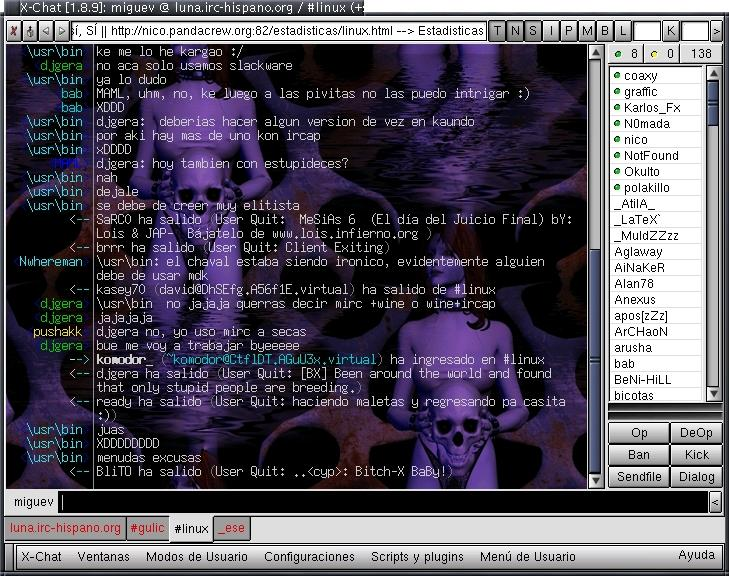
\includegraphics[width=\textwidth]{imagenes/xchat.eps}
% \caption{Cliente de IRC XChat}
% \end{figure}

De la  misma manera, el {\sf  KVirc} es otro cliente  gr�fico capaz de
satisfacer al m�s exigente de  los usuarios. Entre otras cosas destaca
por las ayudas que presta a  aquellos que les gusta disfrutar haciendo
�scripts� para los clientes de IRC

\subsection{Multimedia}
\index{Aplicaciones!multimedia}

La reproducci�n  de los  diferentes formatos gr�ficos  es otro  de los
apartados que se suelen utilizar a  diario. Para los usuarios de otros
sistemas operativos  resulta normal el  poder disponer de  un software
capaz de  reproducir casi  cualquier fichero multimedia.  Sin embargo,
en  Linux ha  costado  un  gran esfuerzo  llegar  a  poder contar  con
reproductores como los que presentamos a continuaci�n.

\subsubsection*{XMMS}
\index{Aplicaciones!XMMS}

{\sf XMMS (X  Multimedia System)} es el reproductor  multimedia de uso
general  en GNU/Linux.  Puede reproducir  cualquier formato  de audio,
tom�ndolo incluso de la red, y  algunos formatos de v�deo MPEG. Adem�s
dispone  de  multitud  de  plugins:  efectos  visuales,  drivers  para
diferentes formatos  de entrada/salida,  y cosas tan  variopintas como
controlarlo mediante un  receptor de infrarojo casero  conectado en el
puerto serie de tu ordenador.

% \begin{figure}[hbtp]
% \centering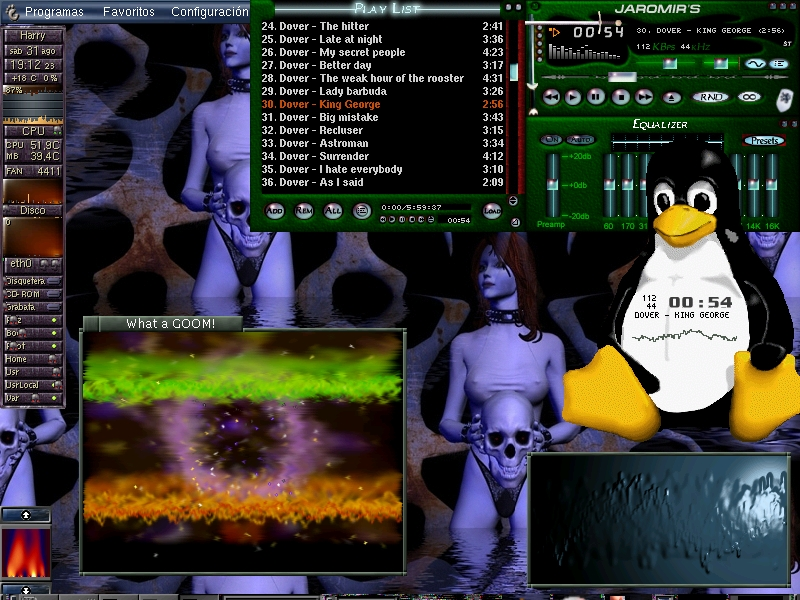
\includegraphics[width=\textwidth]{imagenes/xmms.eps}
% \caption{XMMS con varios plug-ins de visualizaci�n activados}
% \end{figure}

\subsubsection*{Xine}
\index{Aplicaciones!xine}

{\sf Xine} es el resultado de un esfuerzo continuado de superaci�n por
parte  de  la  comunidad  que  lo desarrolla.  Cuando  se  comenz�  su
desarrollo, nadie esperaba  que alcanzara el nivel de  calidad del que
disfruta hoy d�a. Con {\sf Xine} puedes ver pel�culas en formato MPEG,
ASF o DivX 5.

% \begin{figure}[hbtp]
% \centering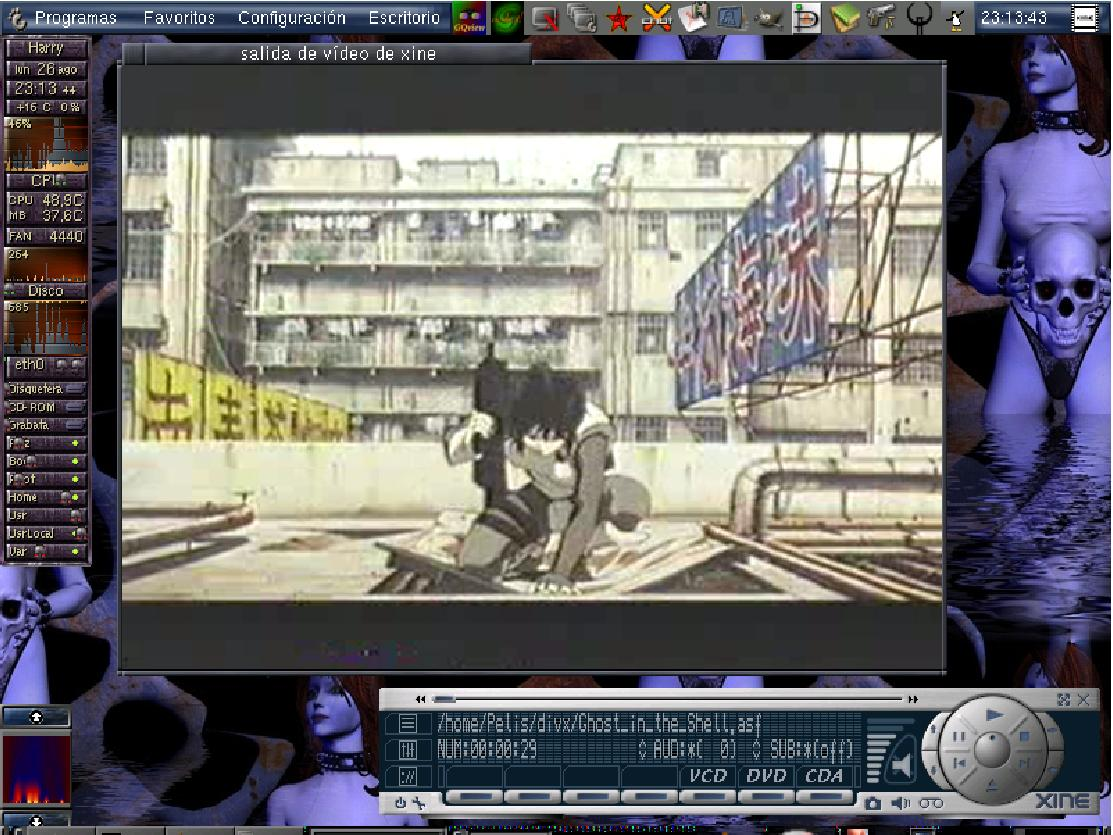
\includegraphics[width=\textwidth]{imagenes/xine.eps}
% \caption{Xine reproduciendo la pel�cula ``Ghost in the Shell''}
% \end{figure}

%\subsubsection*{Aviplay}

\subsubsection*{mpg321} 
\index{Aplicaciones!mpg321}
% <MojoPiKon> Me la pido :-)

{\tt mpg321} es  un reproductor de ficheros con formato  MP3. Se trata
de  un programa  de l�nea  de comandos  no interactivo,  esto es,  uno
ejecuta el programa con una serie de argumentos, y una vez el programa
comienza a  ejecutarse, no  existe interacci�n entre  el usuario  y el
programa, sino que  se limita a realizar las operaciones  que le hemos
proporcionado en la l�nea de comandos.

La forma  m�s asequible  para reproducir  MP3 con  {\tt mpg321}  es el
siguiente  comando, suponiendo  que nos  encontremos en  un directorio
que contenga ficheros MP3.

\begin{verbatim}
$ mpg321 *.mp3
\end{verbatim}

Para aquellos que no les basta esto, hay una amplia gama de par�metros
que pueden pasarse a {\tt mpg321}:

\begin{verbatim}
$ mpg321 -o tipo_de_dispositivo fichero_mp3
\end{verbatim}

\noindent donde tipo  de dispositivo puede ser oss, alsa,  esd, sun, o
arts.

Esto, que en principio no tiene  inter�s alguno para la mayor parte de
la  gente (pues  {\tt mpg321}  funcionar� (en  la mayor  parte de  los
casos)  sin especificar  este  par�metro,  puede resultar  interesante
en  caso de  que,  por  ejemplo, queramos  reproducir  dos  o m�s  MP3
simult�neamente.

Si tenemos {\sf  artsd} instalado, podemos hacer  esto arrancando {\tt
mpg321} de la forma:

\begin{verbatim}
$ mpg321 -o arts fichero.mp3
\end{verbatim}

tras lo cual  podemos repetir la operaci�n tantas  veces como queramos
en la misma o en diferentes consolas.

Este par�metro (-o) funciona conjuntamente con el siguiente:

\begin{verbatim}
$ mpg321 -a nombre_de_dispositivo fichero_mp3 
\end{verbatim}

\noindent donde  {\tt nombre\_de\_dispositivo}  es algo as�  como {\tt
/dev/dsp}, {\tt  /dev/sound/dsp1}, o aquel que  utilice el dispositivo
de sonido que queramos utilizar para oir nuestros MP3 :-)

Utilizaci�n de listas de reproducci�n:

Podemos cargar una ``playlist'' de un  fichero TXT con las rutas a los
ficheros MP3 que queramos que la compongan. Esto se hace de la forma:

\begin{verbatim}
$ mpg321 -@ fichero.txt
\end{verbatim}

Reproducci�n aleatoria de ficheros:

Para esto  tenemos dos par�metros: -z  y -Z; {\tt -Z}  reproduce todos
los ficheros especificados  de forma aleatoria hasta  que paremos {\tt
mpg321}, {\tt -z} reproduce todos  los ficheros especificados de forma
aleatoria una sola vez.

Para  aquellos  que  crean  que   una  aplicaci�n  no  interactiva  de
reproducci�n de MP3 puede  ser totalmente in�til, existen alternativas
en  modo  texto, como  {\tt  mp3blaster}  (tambi�n reproduce  ficheros
ogg-vorbis, el formato libre alternativo  al mp3, que por el contrario
est� patentado y es propietario de Fraunhoffer).

Para el entorno {\sf X-Window}, tenemos {\sf XMMS}, que es un perfecto
clon de  {\sf Winamp},  el conocido reproductor  MP3 para  ese sistema
operativo que todos conocen.

\subsection{Ofim�tica}

Otra �rea compleja de abordar en su  momento, fue la de la creaci�n de
un entorno ofim�tico del nivel adecuado al que ya gozaban los usuarios
de otros sistemas operativos. Esta  tarea aparec�a como inabordable en
unos primeros  momentos, pero s�lo era  una cuesti�n de tiempo  el que
�La  Comunidad� aportar�  los recursos  adecuados para  conseguir este
tipo de  entornos. El resultado  es que  hoy d�a disponemos  de varias
alternativas  para poder  enfrentarnos a  la  dura tarea  de abrir  un
editor de  textos al m�s  puro estilo {\sf Word}  o abrir una  hoja de
c�lculo similar al programa {\sf Excel}.

%\subsubsection*{Koffice}
% \subsubsection*{OpenOffice}
% \index{Aplicaciones!OpenOffice}

% {\sf OpenOffice} es, sin duda,  el proyecto m�s ambicioso, relacionado
% con  la ofim�tica,  que tenemos  en  marcha hoy  en d�a  dentro de  la
% comunidad de desarrolladores de Software Libre.

% {\sf OpenOffice} abarca  todo lo que se puede desear  dentro del campo
% de la ofim�tica de base, cubriendo sobradamente las necesidades reales
% de cualquier usuario de Linux dentro de una empresa. Como este tema ya
% se  trata  en el  tema  \ref{openoffice},  nos limitaremos  a  exponer
% algunas  capturas  de  pantalla  de los  diferentes  m�dulos  de  {\sf
% OpenOffice}.

%(Poner captura del Procesador de Textos)
%(Poner captura de la Hoja de C�lculo)
%(Poner captura del equivalente al PowerPoint)
%(Poner captura de la parte de acceso a Datos)
%(Poner otras capturas)


% \subsection{Gr�ficos}
% \index{Aplicaciones!Gr�ficos}
%\subsubsection*{Gimp}

%\subsubsection*{eog}

%\subsubsection*{gqview}

\subsubsection*{Ghostview}
\index{Aplicaciones!Ghostview}

{\sf  Ghostview}   es  una   interface  de   usuario  X11   para  {\sf
Ghostscript}, que  te permite ver  y navegar por  ficheros PostScript.
Hay diversos derivados de {\sf Ghostview} que son de uso frecuente:

{\sf  Gv} es  una  versi�n de  {\sf Ghostview}  con  una interface  de
usuario mejorado y con capacidad para abrir ficheros PDF.

{\sf MGv}  es un  front-end  basado en  Motif  para {\sf  Ghostscript}
{\sf basado en Ghostview 1.5}.

Hay un programa similar llamado  {\sf GSview} que est� disponible para
usarlo bajo Linux/X11,  Windows y OS/2, pero no est�  derivado de {\sf
Ghostview}.

Algunas caracter�sticas de {\sf Ghostview} son:

\begin{enumerate}

\item {\sf  Ghostview} analiza  todas las  versiones conocidas  de las
{\sf Convenciones de Estructuraci�n de Documentos de Adobe}.

\item El tama�o de la p�gina  se determina autom�ticamente a partir de
los comentarios de estructuraci�n del documento.

\item El usuario puede anular los valores desde los comentarios.

\item El  tama�o de la  ventana se establece  en el cuadro  de l�mites
para los valores del PostScript Encapsulado.

\item El tama�o  por defecto de la p�gina es  Letter y puede cambiarse
mediante {\tt Xresources} o en el  fichero de aplicaci�n por defecto a
A4 (o a cualquier tama�o v�lido).

\item Las barras desplegables aparecen s�lo cuando se necesitan.

\item La orientaci�n  de la p�gina se  determina autom�ticamente desde
los  comentarios de  estructuraci�n  del documento.  El usuario  puede
ignorar los valores.

\item Capacidad para ver  en cuatro orientaciones: Vertical, apaisado,
inversa y apaisado a la derecha.

\item Capacidad para  restringir la presentaci�n a escala  de grises o
monocromo (Requiere {\sf Ghostscript 2.6.1})

\item Capacidad para marcar p�ginas para imprimir o guardar.

\item Puede  mostrar ventanas de  zoom iguales  a la resoluci�n  de la
impresora (1 punto mostrado = 1 punto de impresora).

\end{enumerate}

Aconsejamos poner  GNU {\sf Ghostscript 2.6.2}  que resuelve problemas
de versiones anteriores.

Una  vez  que  tengas  instalado {\sf  Ghostscript}  s�lo  tienes  que
lanzarlo y  en {\tt  abrir documento}  poner la  ruta donde  tengas el
documento PostScript o PDF que quieras visualizar.

%\subsection{Desarrollo}

%\subsubsection*{Glade/Kdevelop}

%\subsubsection*{Cervicia/gcvs}

%\subsubsection*{Quanta/Bluefish}

\subsection{Editores}
\index{Aplicaciones!editores}

%\subsubsection*{AbiWord}

\subsubsection*{KWrite}
\index{Aplicaciones!KWrite}

{\sf KWrite} es un editor de texto para {\sf KDE 2.0}, pero tambi�n es
m�s que  un editor de  textos, pues es  un editor de  programaci�n que
puede considerarse como  una alternativa parcial a  otros editores m�s
poderosos. Es  mejor usarlo  en combinaci�n  con {\sf  Konqueror} como
visor de ficheros en distintos lenguajes.

Una de las principales caracter�sticas  de {\sf KWrite} es la sintaxis
coloreada, adaptada  para muchos lenguajes de  programaci�n tales como
C/C++, Java, Python, Perl, Bash, Modula 2, HTML y Ada.

{\sf KWrite}  es muy  simple de  usar y cualquiera  que haya  usado un
editor de texto no tendr� problemas con �l.

Arrastrar y  Pegar: {\sf KWrite}  usa el  protocolo de {\sf  KDE} para
Arrastre y  Pegado. Los ficheros  pueden ser arrastrados y  pegados en
{\sf KWrite} desde el Escritorio, {\sf Konqueror} o de cualquier sitio
de FTP abierto en una ventana de {\sf Konqueror}.

Opciones de l�neas de comandos:  {\sf KWrite} puede iniciarse desde el
men� de  programas de {\sf KDE}  o desde el icono  del escritorio, as�
como  desde la  l�nea  de  comandos de  un  terminal.  Hay unas  pocas
opciones �tiles disponibles al hacer esto.

Especificar un fichero:  especificando la ubicaci�n y el  nombre de un
fichero,  {\sf  KWrite} lo  abrir�  (o  lo crear�)  inmediatamente  al
iniciarse. Esta opci�n ser�a algo similar a esto:

\begin{verbatim}
$ kwrite /home/midirectorio/docs/mifichero.txt
\end{verbatim}

Especificar un fichero desde Internet:  El m�todo antes se�alado puede
usarse  para abrir  ficheros de  Internet  (si se  tiene una  conexi�n
activa en ese momento). Por ejemplo:

\begin{verbatim}
$ kwrite ftp://ftp.kde.org/pub/kde/Welcome.msg
\end{verbatim}

Otras opciones de l�neas de comando disponibles:

\begin{description}

\item[{\tt --help}] Lista  de las opciones m�s  b�sicas disponibles en
la l�nea de comandos.

\item[{\tt --help-qt}] Lista de  las opciones disponibles para cambiar
la forma en que {\sf KWrite} interact�a con {\sf Qt}.

\item[{\tt --help-kde}] Lista de las opciones disponibles para cambiar
la forma en que {\sf KWrite} interact�a con {\sf KDE}.

\item[{\tt  --help-all}]  Lista de  todas  las  opciones en  l�nea  de
comandos.

\item[{\tt  --author}] Lista  de los  autores  de {\sf  KWrite} en  la
ventana del terminal.

\item[{\tt --version}] Informaci�n  de la versi�n para  {\sf Qt}, {\sf
KDE} y {\sf KWrite}. Tambi�n disponible con {\tt kwrite -V}

\end{description}

\paragraph{Teclas establecidas}

Muchas de las  teclas establecidas (atajos) pueden  configurarse en el
men� de especificaciones. Por defecto {\sf KWrite} trae las siguientes:

\begin{description}

\item[{\tt  Insert}]  Cambia  entre  el  modo de  Inserci�n  y  el  de
Sobreescribir.

\item[{\tt Flecha izquierda}] Mueve el cursor a la izquierda

\item[{\tt Flecha derecha}] Mueve el cursor a la derecha

\item[{\tt Flecha hacia arriba}] Mueve el cursor una l�nea haci arriba

\item[{\tt Flecha hacia abajo}] Mueve el cursor una l�nea hacia abajo

\item[{\tt P�gina adelante}] Mueve el cursor adelante una p�gina

\item[{\tt P�gina atr�s}] Mueve el cursor una p�gina hacia atr�s

\item[{\tt Retroceso}] Borra el car�cter a la izquierda del cursor.

\item[{\tt Inicio}] Mueve el cursor al principio de la l�nea

\item[{\tt Fin}] Mueve el cursor al final de la l�nea

\item[{\tt Suprimir}]  Borra el  car�cter a la  derecha del  cursor (o
cualquier texto seleccionado)

\item[{\tt S-Flecha  izquierda}] Marca el  texto un car�cter  hacia la
izquierda

\item[{\tt  S-Fleha derecha}]  Marca  el texto  un  car�cter hacia  la
derecha.

\item[{\tt F1}] Ayuda

\item[{\tt S-F1}] �Qu� es esto?

\item[{\tt C-F}] Busca

\item[{\tt F3}] Busca de nuevo

\item[{\tt C-C}] Copia el texto marcado en el portapapeles

\item[{\tt C-M}] Pone un Marcador

\item[{\tt C-N}] Nuevo documento

\item[{\tt C-P}] Imprime

\item[{\tt C-Q}] Salir. Cierra la copia activa del editor.

\item[{\tt C-R}] Sustituye

\item[{\tt C-S}] LLama al comando Guardar

\item[{\tt C-V}] Copia el texto del portapapeles en la l�nea

\item[{\tt C-X}] Borra el texto marcado y lo copia en el Portapapeles

\item[{\tt C-Z}] Deshacer

\item[{\tt C-S-Z}] Rehacer

\end{description}

\paragraph{Entradas del men�}

\begin{description}

\item[{\tt Archivo $\Rightarrow$ Nuevo (C-N)}] Abre un documento nuevo
en el editor. Si hay un  documento activo con cambios no guardados, da
opci�n a guardarlos.

\item[{\tt  Archivo $\Rightarrow$  Abrir (C-O)}]  Abre un  fichero por
medio de una ventana de di�logo  que permite navegar por el sistema de
ficheros y que  funciona como un peque�o gestor  de ficheros. Pulsando
con el rat�n en los directorios  mostrados en la ventana central entra
en los directorios y muestra sus contenidos. Hay un cuadro de entradas
que  puede  usarse para  escribir  la  localizaci�n  y el  nombre  del
fichero; haciendo clic en la flecha  que est� al lado, se puede elegir
de la lista de localizaciones usadas recientemente. Debajo de esto hay
un filtro que de modo  similar puede tener datos entrados directamente
o elegidos de  entre los usados recientemente. El  filtro s�lo permite
ficheros que  permitan que sus  especificaciones sean mostradas  en la
ventana  central.  Si  el  fichero contiene  texto,  tal  como  *.txt,
entonces  s�lo los  ficheros con  extensi�n txt  ser�n visibles  en la
ventana. Debajo del filtro hay una barra de estatus que da informaci�n
sobre el  n�mero de  ficheros y  subdirectorios dentro  del directorio
actual.

La Barra de herramientas, que est� localizada en la parte superior del
cuadro de di�logo,  tiene botones de izquierda y  derecha que permiten
moverse  hacia  adelante y  hacia  atr�s  por directorios  previamente
seleccionados, y  flechas arriba y  abajo que permiten moverse  por el
�rbol de  directorios. El bot�n con  la casita lleva al  directorio de
trabajo  del usuario,  y el  de las  dos flechas  curvas actualiza  la
visi�n del directorio actual. El bot�n con la bandera permite poner un
nuevo marcador en el directorio actual o ir a uno previo.

El  �ltimo  bot�n  de  la  barra  de  herramientas  permite  crear  un
directorio nuevo,  y tambi�n cambiar algunas  especificaciones b�sicas
del cuadro  de di�logo.  Tambi�n hay  un cuadro  de descargas  con una
lista de los directorios m�s frecuentados.

\item[{\tt Archivo  $\Rightarrow$ Abrir  recientes}] Esto es  un atajo
para abrir documentos recientemente guardados. Haciendo clic sobre �l,
se abre una lista al lado del men� con diversos ficheros recientemente
guardados. Haciendo  clic sobre  un determinado  fichero se  abrir� en
{\sf KWrite} (si el fichero a�n est� en la misma localizaci�n).

\item[{\tt Archivo  $\Rightarrow$ Guardar (C-S)}] Guarda  el documento
actual.  Si  ya  ha  sido guardado,  sobreescribir�  el  anterior  sin
preguntar. Si es la primera vez que  se guarda, se inicia el cuadro de
guardar que se desribe m�s abajo.

\item[{\tt  Archivo  $\Rightarrow$  Guardar   como}]  Permite  que  un
documento se  guarde con  un nombre  nuevo. Esto  se hace  mediante el
cuadro de di�logo descrito m�s abajo en la secci�n Abrir.

\item[{\tt Archivo  $\Rightarrow$ Imprimir  (C-P)}] Abre un  cuadro de
impresi�n  que  permite  al  usuario especificar  qu�,  d�nde  y  c�mo
imprimir.

\item[{\tt Archivo  $\Rightarrow$ Nueva vista}] Crea  una nueva imagen
del documento  actual, es decir,  una nueva instancia de  {\sf KWrite}
conteniendo el mismo documento.

\item[{\tt Archivo  $\Rightarrow$ Salir (C-Q)}] Cierra  la ventana del
editor. Si est�n  abiertas m�s de una instancia de  {\sf KWrite} estas
quedar�n abiertas.

\item[{\tt Edici�n $\Rightarrow$ Deshacer (C-Z)}] Se usa para eliminar
o deshacer la acci�n m�s reciente.  Para entender mejor esto, v�ase la
secci�n de Deshacer en este mismo documento.

\item[{\tt Edici�n  $\Rightarrow$ Rehacer  (C-S-Z)}] Rehace  el cambio
m�s reciente que se haya hecho mediante Deshacer.

\item[{\tt  Edici�n  $\Rightarrow$   Historial  de  Deshacer/Rehacer}]
Muestra un  cuadro con una  lista de las  acciones m�s recientes  a la
izquierda y otra  lista de las acciones 'deshechas' a  la derecha. Hay
tambi�n  3 botones  a  la derecha  llamados  Deshacer (Undo),  Rehacer
(Redo) Y Cerrar (Close). Haciendo clic en el bot�n Undo produce que se
deshaga la  acci�n al principio  de la lista  y pondr� esta  acci�n al
principio de la  lista de Redo. Igualmente, al hacer  clic en le bot�n
Redo rehar� la acci�n deshecha y la  mueve al principio de la lista de
Undo. Hay muchas opciones aqu�, que ir�s descubriendo con la pr�ctica.

\item[{\tt Edici�n  $\Rightarrow$ Cortar  (C-X):}] Borra  la selecci�n
actual  y  la  pone  en   el  portapapeles.  El  portapapeles  es  una
caracter�stica  de  {\sf  KDE}  que  opera  de  forma  invisible  para
proporcionar una forma de transferir datos entre aplicaciones.

\item[{\tt  Edici�n  $\Rightarrow$  Copiar  (C-C):}]  Copia  el  texto
seleccionado al Portapapeles de forma que pueda pegarse en otro sitio.

\item[{\tt Edici�n $\Rightarrow$ Pegar (C-V):}] Inserta los contenidos
del Portapapeles en la posici�n del cursor.

\item[{\tt Edici�n $\Rightarrow$ Seleccionar Todo (C-A):}] Seleccional
todo el  documento. Es muy  �til para copiar  todo el fichero  en otra
aplicaci�n.

\item[{\tt Edici�n  $\Rightarrow$ Invertir la  Selecci�n:}] Selecciona
el  texto no  seleccionado  y ``deselecciona''  texto ya  seleccionado
-revirtiendo el estado actual de la selecci�n.

\item[{\tt Edici�n $\Rightarrow$ Ir a l�nea (C-G):}] Abre un cuadro de
dialogo de ``ir  a linea'' que se  usa para que el cursor  salte a una
l�nea particular (especificada por su n�mero) del documento. El n�mero
de la  l�nea puede entrarse  directamente en el  cuadro de texto  o de
forma gr�fica  haciendo clic en  los controles  al lado del  cuadro de
texto. La flechita  hacia arriba incrementa los n�meros de  l�nea y la
flechita hacia abajo los disminuye.  Tambi�n hay un control deslizante
a la derecha del texto que permite moverse de manera an�loga.

\item[{\tt Edici�n $\Rightarrow$ Encontrar  (C-F):}] Abre un cuadro de
di�logo  que  sirve  para  especificar  el texto  a  encontrar  en  el
documento. En el cuadro de texto puede entrarse un patr�n de b�squeda.
Tambi�n permite  tener disponibles b�squedas  recientes. Seleccionando
el que tome  en cuenta may�sculas/min�sculas limita la  b�squeda a eas
especificaciones.  Hay muchas  otras  utilidades en  este comando  que
descubrir�s con la pr�ctica.

\item[{\tt Edici�n $\Rightarrow$ Encontrar siguiente (F3):}] Repite la
�ltima  operaci�n de  b�squeda  sin  llamar al  cuadro  de di�logo  de
Encontrar.

\item[{\tt Edici�n $\Rightarrow$ Encontrar  Previo (S-F3):}] Repite la
anterior operaci�n  de b�squeda,  sin llamar al  cuadro de  di�logo de
Encontrar.

\item[{\tt Edici�n $\Rightarrow$ Sustituir  (C-R):}] Abre un cuadro de
di�logo de  Sustituir, que  es casi id�ntico  al de  Encontrar. Adem�s
contiene una opci�n de ``Sustituir  con'' que puede usarse para buscar
un texto seleccionado y sustituirlo  por otro seleccionado tambi�n. La
opci�n de confirmar  la sustituci�n permite que  {\sf Kwrite} pregunte
antes de cada sustituci�n.

\item[{\tt Edici�n  $\Rightarrow$ Comando de edici�n  (C-M):}] Comando
de editar.

\item[{\tt Marcadores $\Rightarrow$ (C-B):}] Bot�n de Marcadores

\item[{\tt Marcadores  $\Rightarrow$ Borrar Marcadores:}]  Borra todos
los marcadores  del documento as� como  la lista de matcadores  que se
a�ade al final de este �tem del men�.

\item[{\tt Herramientas $\Rightarrow$ Ortograf�a:}] Inicia el programa
de  revisi�n  ortogr�fica, dise�ado  para  ayudar  a corregir  errores
tipogr�ficos.  Tiene   3  cuadros   de  texto  aobre   ``palabras  mal
escritas'',  ``sustituci�n'' y  ``suegerencias'' que  son muy  �tiles.
Adem�s hay  otro cuadro  de di�logo  a la derecha  con 6  botones para
``sustituir'',  ``sustituir  todo'',  ``ignorar'',  ``ignorar  todo'',
``a�adir''  y  ``parar''. Tambi�n  tiene  una  barra de  progreso  que
permite comprobar por  d�nde va el proceso de  correcci�n. Hay tambi�n
otros  dos botones:  Ayuda y  Cancelar que  abren el  men� de  ayuda y
cancelan el proceso de correcci�n respectivamente.

\item[{\tt  Herramientas   $\Rightarrow$  Indentar:}]   Incrementa  la
indentaci�n (tabulaciones)  del p�rrafo  un paso.  El tama�o  del paso
depende de lo que se haya establecido.

\item[{\tt   Herramientas  $\Rightarrow$   Desindentar:}]  Reduce   la
indentaci�n del p�rrafo un paso.

\item[{\tt  Herramientas $\Rightarrow$  Quitar  Indentaci�n:}] A�n  no
est� implementado.

\item[{\tt Herramientas $\Rightarrow$ Comentar:}]  A�ade un espacio al
comienzo de la l�nea donde est� el  cursor o al comienzo de las l�neas
seleccionadas.

\item[{\tt  Herramientas   $\Rightarrow$  Descomentar:}]   Elimina  un
espacio (si lo hay) al comienzo de  la l�nea donde est� el cursor o al
comienzo de las l�neas seleccionadas.

\item[{\tt Herramientas $\Rightarrow$ Indentar (C-I):}] Indenta

\item[{\tt Herramientas $\Rightarrow$  Desindentar (C-U):}] Deshace la
indentaci�n.

\item[{\tt Herramientas  $\Rightarrow$ Quitar Indentaci�n:}]  Quita la
indentaci�n.

\item[{\tt Herramientas $\Rightarrow$ Comentar (C-\#):}] Comenta

\item[{\tt   Herramientas    $\Rightarrow$   Descomentar   (C-S-\#):}]
Descomenta.

\item[{\tt    Configuraci�n    $\Rightarrow$    Muestra    Barra    de
Herramientas:}] Muestra una barra de herramientas movible que contiene
botones usados para iniciar  comandos frecuentemente usados. Cuando no
se usa, est� oculta.

\item[{\tt  Configuraci�n  $\Rightarrow$  Muestra Barra  de  Estado:}]
Muestra una peque�a barra al final del editor que contiene informaci�n
sobre el estatus del documento actual. Permanece oculta si no se usa.

\item[{\tt Configuraci�n $\Rightarrow$  Muestra localizaci�n:}] Cuando
se selecciona, muestra la localizaci�n  del documento en el sistema de
ficheros. Si no se usa, est� oculta.

\item[{\tt  Configuraci�n  $\Rightarrow$   Configura  asociaciones  de
teclas:}] Abre  un cuadro  de di�logo que  permite cambiar  las teclas
asociadas a  funciones. La  ventana muestra la  lista de  acciones que
pueden realizarsae mediante teclas. Una utilidad muy interesante y que
tiene muchas posibilidades a explorar.

\item[{\tt    Configuraci�n   $\Rightarrow$    Configura   Barra    de
herramientas:}] Abre un cuadro de di�logo que permite cambiar la barra
de herramientas de configuraci�n. Otra  opci�n interesante que hay que
explorar.

\item[{\tt Configuraci�n $\Rightarrow$ Configura  el Editor:}] Abre un
cuadro de di�logo que permite ajustar las configuraciones.

\item[{\tt Configuraci�n  $\Rightarrow$ Muestra los l�mites  del Icono
(F6):}] Pone un l�mite a la  izquierda de la ventana de edici�n, donde
se muestran los marcadores junto a la l�nea a los que se aplican.

\item[{\tt Configuraci�n  $\Rightarrow$ Selecci�n Vertical  (F4):}] Se
usa para activar o desactivar una selecci�n. Permite seleccionar texto
por filas y por columnas.

\item[{\tt  Configuraci�n $\Rightarrow$  Modo  de Resaltar:}]  Permite
elegir  el  estilo de  colores  que  se  usa  para mostrar  el  texto.
Los  estilos  se seleccionan  mediante  lenguaje  de programaci�n.  La
informaci�n sobre la fuente/color no se almacena con el documento.

\item[{\tt Configuraci�n $\Rightarrow$ Fin de L�nea:}] Abre un submen�
que permite seleccionar el tipo de c�digo de ``fin de l�nea'' que debe
usar  {\sf KWrite},  esto es,  los est�ndares  aceptados por  sistemas
UNIX, Mac o MSDOS/Windows.

\item[{\tt Ayuda $\Rightarrow$ Contenidos  (F1):}] LLama al sistema de
ayuda de {\sf KDE} y a las p�ginas de ayuda de {\sf KWrite}.

\item[{\tt  Ayuda  $\Rightarrow$ �Qu�  es  esto?  (S-F1):}] Cambia  el
puntero del rat�n a una flecha con un {\tt ?}. Haciendo clic sobre los
�tems abre una ventana de ayuda que explica su funci�n.

\item[{\tt Ayuda $\Rightarrow$ Informes de Fallos:}] Abre un cuadro de
di�logo  que permite  ayudar  al  equipo de  {\sf  KDE}  a rastrear  y
solucionar fallos mediante correo  electr�nico con la informaci�n dada
por el usuario.

\item[{\tt  Ayuda $\Rightarrow$  Sobre  KWrite:}] Muestra  informaci�n
sobre la versi�n y el autor.

\item[{\tt Ayuda $\Rightarrow$ Sobre KDE:}] Muestra informaci�n b�sica
sobre la versi�n de {\sf KDE}.

\end{description}

\paragraph{Configuraci�n de KWrite}

Seleccionar  {\tt Configuraciones  $\Rightarrow$ Configura  el Editor}
desde  el men�,  abriendo un  cuadro de  di�logo de  Configuraci�n del
Editor.  Puede usarse  para  cambiar  diferentes configuraciones,  que
est�n disponibles dependiendo de lo que  se elija de la lista vertical
o a la izquierda del cuadro de  di�logo. Se puede llamar al sistema de
Ayuda, aceptar  la configuraci�n actual  y cerrar el cuadro  por medio
del bot�n de  {\tt OK} o {\tt Cancelar el  proceso}. Las categor�as de
Colores, Fuentes Indentado, Selecci�n,  Editar, Comprobar ortograf�a y
Resaltado se detallan m�s abajo.

\begin{description}

\item [Colores] Proporciona acceso a dos diferentes configuraciones de
color haciendo  clic sobre  el bot�n correspondiente,  que llama  a un
cuadro de  di�logo que se  usa para cambiar las  especificaciones. Hay
muchas cosas interesantes por hacer al explorar esta funci�n.

\item [Fuentes] Permite elegir la  fuente por defecto de {\sf KWrite}.
Se puede elegir cualquier fuente disponible  en el sistema y poner por
defecto  un tama�o  y  un tipo  de codificaci�n.  Hay  una ventana  de
muestra que permite ver el efecto de los cambios.

\item  [Indentado]

\begin {description}

\item 

\item [El Auto  Indentado] hace que las nuevas l�neas  empiecen con el
mismo nivel de indentaci�n que las anteriores.

\item [Indentado con Espacios] sustituye el tabulador por el n�mero de
espacios  seleccionado en  la ventana  de  Ancho del  Tabulador de  la
secci�n de Edici�n del Cuadro de Preferencias.

\item [Indentado con  la tecla de retroceso] permite usar  la tecla de
retroceso para indentar.

\item [Indentado  con la tecla  de Tabulador] permite usar  esta tecla
para indentar.

\item  [Mantener espacios  extras]  las indentaciones  mayores que  un
n�mero seleccionado de espacios no ser�n reducidas.

\end{description}

\item  [Selecci�n]
\begin{description}

\item 

\item [Selecciones Permanentes] impide que al pulsar una tecla o mover
el cursor se elimine una selecci�n de texto.

\item  [Sobreescribir Selecciones]  cualquier entrada  de un  car�cter
pulsado o una operaci�n de pegado sustituir� el texto seleccionado.

\item [Autocopia  con el  rat�n] cualquier  texto seleccionado  con el
rat�n se copiar� autom�ticamente en el Portapapeles.

\item [Selecci�n Vertical] activa la selecci�n vertical.

\end{description}

\item [Editar] 
\begin{description}

\item 

\item  Mover Palabra:  es una  caracter�stica que  hace que  el editor
empiece autom�ticamente una nueva l�nea de  texto y mueva el cursor al
principio de  la nueva  l�nea. {\sf KWrite}  comenzar� autom�ticamente
una l�nea  nueva de texto cuando  la l�nea actual alcance  la longitud
establecida en la opci�n Mover palabra en.

\item Mover palabra en: si  est� seleccionada la opci�n anterior, esta
entrada determina la  longitud (en caracteres) a partir de  la cual el
editor empieza autom�ticamente una  nueva l�nea. Sustituir Tabuladores
por

\item  Espacios: {\sf  KWrite} sustituir�  cualquier tabulador  por el
n�mero de espacios que se le indique en Ancho de Tabuladores.

\item Remover Espacios sobrantes: {\sf KWrite} elimina autom�ticamente
los espacios  extra al final  de las l�neas de  texto. Autopar�ntesis:
cuando  se pulsa  el par�ntesis  izquierdo (\verb|[|  o \verb|{|  {\sf
KWrite}  automaticamente  coloca  el  derecho  \verb|}|,  \verb|)|,  o
\verb|]| a  la derecha del cursor.  Hay muchas otras opciones  en este
men� como  Deshacer grupos  o Mostrar  Tabuladores que  es interesante
explorar.

\end{description}

\item [Ortograf�a]  Un corrector  ortogr�fico es un  programa dise�ado
para ayudar  al usuario  a detectar  y corregir  errores tipogr�ficos.
Permite  que se  ajusten  em las  preferencias importantes  funciones,
como  Crear  combinaciones  de  ra�ces/sufijos  que  no  est�n  en  el
Diccionario, lo  que permite  al corrector registrar  como `correctas'
las combinaciones de palabras ra�ces  con sufijos o prefijos aunque no
est�n en la  base de datos del diccionario.  Hay diversos diccionarios
seg�n  el idioma  seleccionado.\\ {\sf  Codificaci�n:} hay  diferentes
sistemas de  codificaci�n que pueden  activarse para que  el corrector
haga su trabajo adecuadamente. Como {\sf KWrite} no contiene su propio
corrector, se ha de elegir uno externo para su uso.

\item  [Resaltado]  hay  dos  aspectos:  los  que  est�n  por  defecto
y  los  modos  de resaltado.  En  la  secci�n  de  los que  est�n  por
defecto, est�n  los estilos por  defecto de la apariencia  de diversos
�tems,  los  distintos  elementos  que se  quieran  resaltar  (normal,
comentario, negrita, cursivas, texto  seleccionado, etc). En los modos
de resaltado, no hay que establecer  cada una de las opciones dado que
los no  se configuren  espec�ficamente usar�n las  configuraciones por
defecto.  Adem�s,  los estilos  de  resaltado  para cada  lenguaje  de
programaci�n o  la sintaxis a  destacar, etc. Hay muchas  opciones que
permiten facilitar  el trabajo  de programaci�n que  hacen interesante
explorar estas opciones.

\end{description}

Con  esta   peque�a  Gu�a  s�lo   se  han  mostrado  algunas   de  las
caracter�sticas m�s importantes  y b�sicas de {\sf  KWrite}. El manual
de {\sf KWrite} y la pr�ctica con el programa completar�n los aspectos
que aqu� no han sido tratado expl�citamente.


\subsubsection*{gnotepad}
\index{Aplicaciones!gnotepad}

{\sf Gnotepad+} es un  editor de textos y de HTML,  f�cil de usar pero
muy completo para sistemas basados en UNIX que dispongan de X11 y usen
{\sf  GTK (Gimp  ToolKit)} o  {\sf GNOME}.  {\sf Gnotepad+}  se dise��
para  ser  liviano  y  al  mismo tiempo  proporcionar  muchos  de  las
caracter�sticas comunes de los modernos  editores de textos basados en
{\em GUI (Graphical User Interface)}.

Algunas  de las  caracter�sticas de  {\sf Gnotepad+}  son: ventanas  y
documentos m�ltiples;  di�logos de edici�n e  inserciones de etiquetas
de HTML; deshacer y rehacer  ilimitados; men� de documentos recientes;
ventanas emergentes de listas de documentos, de ventanas y de cajas de
mensajes; autoguardado  de documentos;  arrastre y pegado  de ficheros
entre {\sf Gnotepad+} y otras aplicaciones.

En la  web de  {\sf Gnotepad+}  {\tt http://gnotepad.sourceforge.net/}
encontrar�s  diversas  capturas  de  pantalla de  {\sf  Gnotepad+}.  A
continuaci�n ponemos algunas como muestra de las posibilidades de este
potente editor  de textos.  Como sucede  en el  mundo Linux,  entre el
manual y la documentaci�n que est�  disponible en tu distribuci�n y la
pr�ctica con el programa, en poco tiempo descubrir�s sus ventajas y lo
adecuar�s a la medida de tus necesidades.

%\begin{figure}[hbt]
%\centering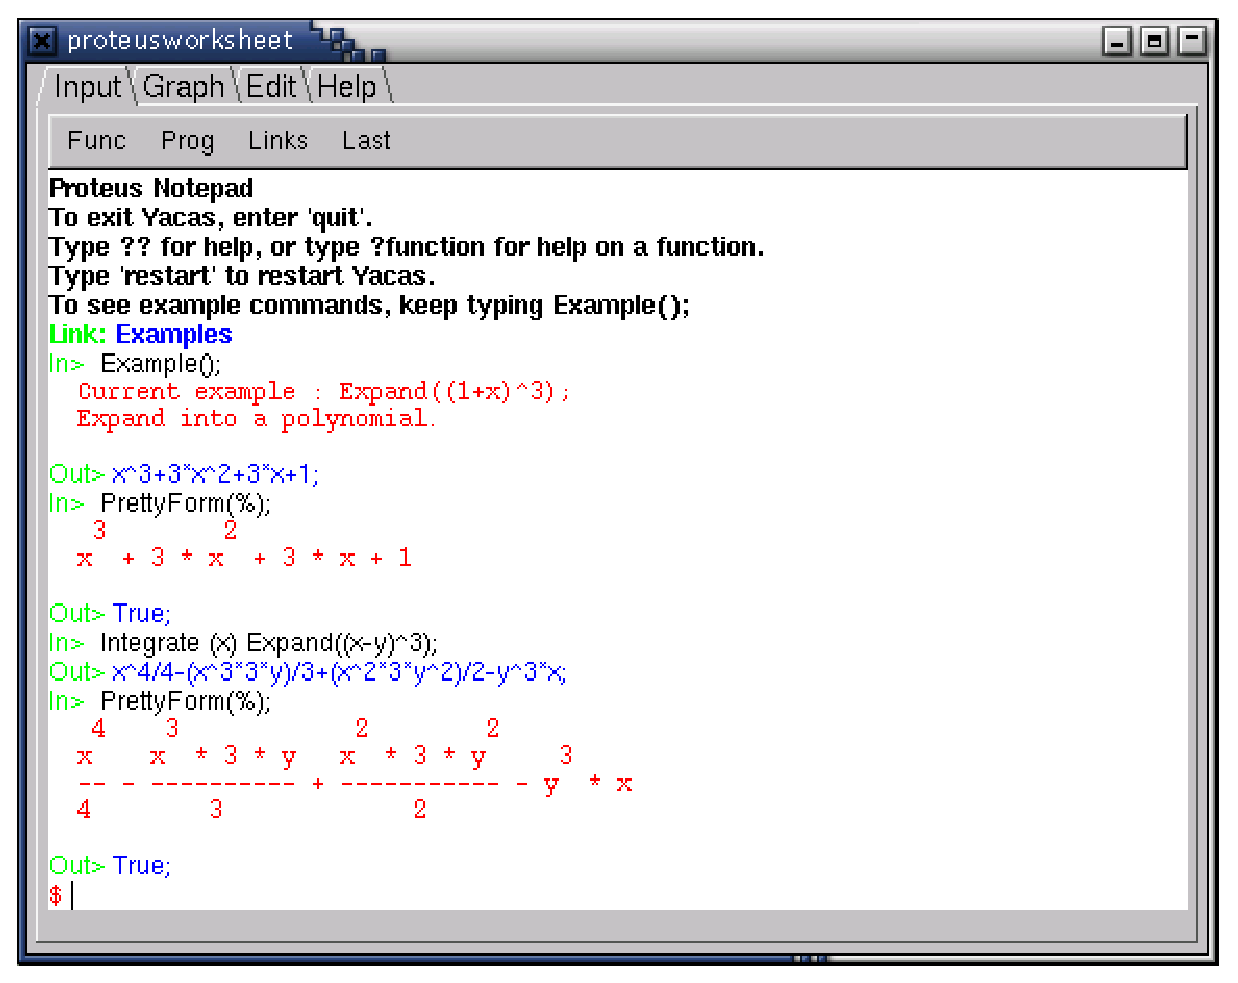
\includegraphics[width=0.65\textwidth]{imagenes/proteus.eps}
%\caption{Proteus, interfaz gr�fica para Yacas}
%\end{figure}

%\subsubsection*{Kwordtrans}

%\subsection{Sistema}
%\subsubsection*{gmemusage}
%\subsubsection*{gr_monitor}

%\subsection{Aplicaciones en general}
%\subsubsection*{Creaci�n de CD's}
%\paragraph*{GCombust}
%\paragraph*{XCDRoad?}
%\paragraph*{KreateCD}
%\paragraph*{Kover}

%\subsubsection*{Por Definir}

%% Segunda secci�n
% \section{Aplicaciones no Gr�ficas}

% Se  puede  afirmar  que  por cada  aplicaci�n  gr�fica  disponible  en
% Linux,  tenemos 50  utilidades  disponibles desde  la terminal.  Estas
% aplicaciones son  el verdadero motor  de todos los  sistemas derivados
% de  UNIX. Con  ellas  se  pueden llevar  a  cabo  infinidad de  tareas
% importantes, desde ordenar  cualquier tipo de archivo  de datos, hasta
% programar  el  encendido  de  una cafetera  para  cuando  nos  estemos
% quedando dormidos. Todas ellas pueden  ser lanzadas desde una terminal
% en modo gr�fico, de manera que tambi�n las podemos utilizar desde este
% entorno.

%\subsection{Desarrollo}
%\subsubsection*{GCC}
%\subsubsection*{make}
%\subsubsection*{gettext}

%\subsection{Editores}
%\subsubsection*{emacs}
%\subsubsection*{vim}

%\subsection{Gr�ficos}
%\subsubsection*{ImageMagick}
%\subsubsection*{Otros Filtros}

%\subsection{Internet}
%\subsubsection*{iptraf}
%\subsubsection*{ntop}

%\subsubsection*{aumix}
%\subsubsection*{zgv}
%\subsubsection*{aatv}

%\subsection{Ofim�tica}
%\subsubsection*{bc}
%\subsubsection*{}

%\subsection{Sistema}
%\subsubsection*{top}
%\subsubsection*{crontab}
%\subsubsection*{at}
%\subsubsection*{uptime}

%Autor: amd77
%amd77: 7

\chapter{Documentacion y ayuda}
\label{documentacion.tex}
\label{documentacion}
\index{Documentación}
\index{Ayuda}

El primer  contacto con un entorno  nuevo como Linux siempre  se suele
hacer junto a alguien  que te oriente (al que de  ahora en adelante me
referiré con el término {\em gurú de turno}). Cuando ese gurú vuelve a
sus tareas cotidianas normalmente te quedas solo y te toca buscarte la
vida. En este capítulo veremos diferentes formas con las que conseguir
el conocimiento  suficiente para poderse  buscar la vida solo  y hasta
convertirte en un  gurú también, pues eso  es lo que él  ha hecho para
saber lo que sabe. Veremos que  una gran parte ya lo tienes almacenado
en tu disco  duro tras instalar Linux, y te  diremos cómo conseguirlo,
mientras que  el que  te falte  lo podrás  encontrar en  la red,  y te
diremos dónde buscarlo.

\section{Pasos para encontrar ayuda}

Estos pasos  son para cuando  no sabes  como funciona un  programa. Si
realmente lo  que pasa  es que  no entiendes  nada, deberías  pasar al
siguiente punto, Recursos, donde se detallan guías y tutoriales. Estos
pasos que aquí se detallan están en orden de dificultad creciente.

\subsection{Información en línea de comandos}
\index{Ayuda!--help}

Cada comando en Linux siempre está  documentado, ya sea de una forma u
otra. Cuando  conocemos un comando  y no  sabemos lo que  hace nuestra
primera  opción puede  ser llamar  al  comando con  el argumento  {\tt
--help} o  {\tt -h},  con lo  que en la  mayoría de  los casos  se nos
mostrará un pequeño resumen  de su uso y de la  forma de llamarlo, con
lo que nuestras  dudas comenzarán a disiparse. Este es  un estándar de
facto bastante extendido.

\subsection{Páginas del manual}
\index{Documentacion!man}

Si aún así  seguimos con dudas, o si queremos  ver una descripción más
pormenorizada de lo que hace cada uno de los parámetros de que dispone
el comando, probaremos si el comando dispone de {\em página de manual}
tecleando {\tt  man comando}.  En caso  afirmativo, nos  aparecerá una
descripción más detallada  del comando, comenzando por  un resumen, la
descripción de la sintaxis, del  funcionamiento, de las opciones y por
último  información  de  bugs,  ficheros  relacionados  y  referencias
cruzadas. Desde  los primeros UNIX las  páginas de manual han  sido el
principal  medio de  documentación  sobre comandos  concretos y  todas
coinciden en los mismos contenidos mencionados anteriormente.

Algo que debemos  tener en cuenta es que debido  también a la herencia
UNIX,  el primer  idioma en  que  se escriben  todos estos  documentos
técnicos suele ser  el inglés, por ser el idioma  de mayor difusión en
el mundo  de la informática. Cuando  el documento es un  documento muy
usado, entonces voluntarios lo traducen a su idioma nativo. El caso es
que las páginas de manual de  los comandos más usados seguro que están
ya  traducidos  al  español.  Si  nada  en  el  sistema,  ni  siquiera
aplicaciones, aparecen en español, entonces  es posible que haya algún
problema con las variables de entorno del idioma (para más información
consultar {\tt man setlocale}). Si hay aplicaciones que sí aparecen en
español,  entonces puede  ser que  estas  páginas de  manual no  estén
instaladas y tengas que hacerlo (depende de la distribución, en Debian
el paquete se llama {\tt manpages-es}).

Relacionados con el comando {\tt man} existen dos comandos. El primero
es  que {\tt  apropos}, que  busca la  palabra que  le decimos  en los
resúmenes  de las  páginas  de  manual instaladas  y  nos muestra  las
páginas que coinciden. El segundo es  de menor utilidad, se llama {\tt
whatis}, y simplemente muestra la línea de descripción del comando, no
la ayuda completa.

Con la llegada de los entornos gráficos, las páginas del manual se han
modernizado también y se han  integrado en los entornos más populares.
En  el caso  del entorno  de escritorio  {\sf KDE},  abriendo un  {\sf
Konqueror} y tecleando  en la barra de dirección  {\tt man:} obtenemos
un listado de todas las páginas de manual organizadas en categorías, o
bien  seguido  de una  barra  y  el  nombre  del comando  nos  aparece
directamente su página,  por ejemplo, {\tt man:/ls}. En  caso de tener
varios idiomas también  aparecen allí. En el caso  del escritorio {\sf
GNOME 1.2}, todo lo tenemos  en la aplicación {\sf Gnome-help-browser}
(sistema integral de ayuda).

\subsection{Páginas info}
\index{Documentacion!info}

Las  páginas  del manual  para  escribirse  utilizan un  preprocesador
llamado  {\tt  troff}. Con  la  llegada  de  nuevos y  más  versatiles
preprocesadores,  las páginas  del manual  tuvieron la  posibilidad de
vincularse unas con otras, es decir,  disponer de un índice del que se
va a otras páginas  y sobre estas, a su vez, puede  irse a otras, etc:
organizarlas como una obra de  consulta más que como páginas aisladas.
El primer  fruto de  esto fueron  las páginas {\tt  info}, que  son un
sistema de ayuda navegable.  Actualmente los preprocesadores como {\tt
sgmltools} permiten producir formatos de salida info, HTML, y otros, a
partir de  un único texto  de ayuda escrito  por el programador  de la
aplicación, y cualquier ahorro de tiempo es una ventaja.

El visualizador  de páginas info,  igual que man, ha  evolucionado con
los entornos gráficos.  El visualizador con interfaz en  modo texto se
ejecuta  tecleando con  {\tt info}  o bien  {\tt info  comando} si  ya
sabemos  lo que  deseamos ver.  Una  vez dentro,  con tabulador  vamos
recorriendo cada  uno de  los enlaces. Cuando  queremos entrar  en uno
pulsamos {\tt Enter}. La estructura  es jerárquica, en forma de árbol,
y podemos  movernos a los nodos  de arriba ({\tt u}),  siguiente ({\tt
n}) y anterior ({\tt p}).

En modo gráfico, en el escritorio  {\sf KDE}, al igual que las páginas
del manual, simplemente  tecleamos en la barra de  direcciones de {\sf
Konqueror} {\tt info:} para verlo todo,  o bien seguido de una barra y
el nombre  de un  tema concreto, como  por ejemplo,  {\bf info:/libc}.
Para {\sf GNOME 1.2},  la aplicación {\sf Gnome-help-browser} (Sistema
integral de ayuda) nos permite visualizarlo también.

\subsection{Documentación DVI/PS/PDF/HTML}
\index{Documentacion!dvi}
\index{Documentacion!ps}
\index{Documentacion!pdf}
\index{Documentacion!html}

El  siguiente  paso en  documentación  se  dió  con  \LaTeX y  con  la
evolución del {\tt sgmltools} hacia {\sf DocBook}. Con ambos sistemas,
escribir manuales y documentos se  facilita enormemente, y a partir de
un  único  documento  se  pueden  conseguir  versiones  en  diferentes
formatos:

\begin{itemize}

\item {\bf DVI (DeVice Independent file)}: Es el formato de salida del
procesador  \LaTeX.  Sólo  se  usa  en  documentos  sin  imágenes.  Se
visualiza, entre otros, con el programa {\tt xdvi}.

\item  {\bf  PS  (PostScript)}:  Es   un  formato  de  impresión  para
impresoras de  calidad profesional y  resulta muy interesante  pues se
ve  perfecto  tanto en  impresoras  profesionales  como en  impresoras
normales. La visualización en pantalla aparece tal cual va a salir por
impresora. Se puede visualizar con  {\tt gs}, {\tt gv}, {\tt gnome-gv}
({\tt ggv}, para {\sf GNOME}) y {\tt kghostview} (para {\sf KDE}).

\item {\bf  PDF (Portable  Document Format)}:  Es un  formato reciente
similar  al  PostScript,  con  la  desventaja de  que  no  se  imprime
directamente  en las  impresoras, sino  que es  necesario instalar  un
visor. Como  visualizadores libres tenemos  el {\tt xpdf} y  todos los
anteriores  visores  de PostScript.  También  existe  el {\em  Acrobat
Reader} ({\tt acroread}) que no es libre pero sí gratuito.

\item {\bf HTML (HyperText Meta  Language)}: El formato de archivos de
la WWW  resulta interesante para  manuales, pues se puede  publicar en
Internet y al  mismo tiempo lo puedes tener como  paquete instalado en
un directorio de  documentación de tu disco duro para  poder verlo sin
conexión. Suele contener  vínculos que te permiten  navegar por dentro
de todas  las relaciones en el  documento. Se puede ver  con cualquier
navegador de  las docenas de  ellos que  existen para Linux,  tanto en
modo gráfico  como en  modo texto.  Aparte, los  sistemas de  ayuda de
Gnome y  {\sf KDE}, así como  {\tt devhelp} (un sistema  de ayuda para
programadores),  aunque todos  tengan  una interfaz  integrada con  el
escritorio, resulta que usan HTML, por lo que también se pueden ver en
cualquier navegador.

\item {\bf  Texto plano}:  Este formato  puede parecer  obsoleto, pero
sigue  usándose  pues  no  hace  falta ningun  visor  para  verlo.  En
especial, es interesante cuando no tienes entorno gráfico, o cuando no
tienes  navegadores con  los que  visualizar el  resto de  formatos, o
simplemente por ahorrar espacio, pues  al carecer de todos los códigos
de  formato  ocupa notablemente  menos.  Se  visualiza con  un  simple
editor, o bien con {\tt less} o  {\tt zless} si tiene sufijo {\tt .gz}
(compresión {\tt gzip}).

\end{itemize}

\subsection{Documentación del paquete}
\index{Documentacion!del paquete}

Normalmente  usamos  Linux  después  de haber  instalado  una  de  las
distribuciones  existentes. Sea  cual  sea la  distribución, una  cosa
en  la que  se  coincide  es organizar  las  aplicaciones en  paquetes
individuales. Cuando alguien instala uno de esos paquetes, se instalan
los ejecutables y resto de  archivos necesarios para el funcionamiento
de la aplicación, y también las páginas  de manual y de info y también
suele ser común tener un directorio  con el resto de documentación del
paquete.

Recordemos que el  software en Linux es código  abierto, eso significa
que  el programador  distribuye  libremente el  código  fuente de  las
aplicaciones, con el deseo de que sea  útil para más gente. Y para que
esto sea  posible para  el máximo número  de personas,  el programador
siempre  suele  acompañar  junto  al  código  fuente  de  su  programa
instrucciones  de instalación  y  de  uso, así  como  manuales que  no
estén  en formato  man  o info.  Cuando la  gente  de la  distribución
crea  el  ejecutable  a  partir  del código  fuente,  éste  ya  no  es
necesario,  pero como  los archivos  de ayuda  del programador  tienen
información útil  pasan a  colocarse en un  directorio, que  suele ser
{\tt /usr/share/doc/nombredelpaquete}. Cuando  no conseguimos ayuda de
otras formas, no debemos olvidarnos de mirar aquí.

En la  distribución Debian existe  un paquete llamado {\tt  dhelp} que
busca documentos útiles  para el usuario por todos  los directorios de
documentación de paquete y te los indexa y muestra de forma organizada
para un fácil acceso a todos ellos.


\subsection{Recursos en Internet de la distribución}
\index{Documentacion!de la distribucion}

Cada distribución de  Linux construye los ejecutables a  partir de las
fuentes a su manera, y ordena los archivos de configuración y archivos
de ayudas  según su criterio. Posiblemente  las ayudas estén ahí  y no
seamos capaces de encontrarlas.  Simplemente pidiendo ayuda a usuarios
más  veteranos  de  nuestra  misma  distribución  consigamos  resolver
nuestro problema o  duda. Para esto, solo tenemos que  buscar foros en
Internet sobre nuestra distribución, o bien sobre Linux en general. Si
lo que queremos realizar es algo común, muy probablemente otra persona
lo  haya  preguntado  y  ya  ha  sido  contestado,  así  que  buscando
previamente  en  los  archivos  de las  listas  nuestra  pregunta  nos
ahorraremos preguntarlo y evitaremos hacer a la gente preguntas que ya
han  sido  tratadas  y  contestadas.  A  veces,  cuando  los  usuarios
veteranos están cansados de responder  siempre a las mismas preguntas,
se crean  los {\em  FAQ - Frequently  Asked Questions}  (traducido por
{\em  PUF -  Preguntas  de  Uso Frecuente}),  que  son colecciones  de
preguntas/respuestas muy típicas y útiles para cualquiera.

Por ejemplo,  para la distribución  Debian, el sitio donde  ponerse en
contacto con usuarios veteranos es  vía lista de correo (una dirección
de correo  electrónico a la  que se pueden suscribir  muchas personas)
{\tt  debian-user-spanish@lists.debian.org}  o  bien en  el  siguiente
foro:  {\tt  http://www.esdebian.org/}.  Para obtener  FAQ's  y  otros
documentos en: {\tt http://www.debian.org/doc/index.es.html}


\subsection{Recursos en Internet del programa}
\index{Documentacion!del programa}

En caso que nuestras pretensiones de conocer el programa sean mayores,
o que  las anteriores búsquedas  hayan sido infructuosas,  siempre nos
queda la  opción de buscar  la página web  de la aplicación.  Como las
aplicaciones  libres  viven de  su  difusión,  el programador  siempre
intenta disponer de  una página web donde se anuncie  su programa, las
nuevas versiones, su dirección de correo donde comunicar bugs, enlaces
con ayudas y  tutoriales, listas de correo donde  ser notificado sobre
las  actualizaciones  o  donde  los usuarios  de  su  programa  pueden
discutir, ayudarse  unos a los  otros o proponer mejoras  al programa.
Mirando en el directorio de  documentación del programa o tecleando el
nombre de la aplicación en un buscador nos puede llevar a esta página.


\subsection{Código fuente}
\index{Documentacion!codigo fuente}

Una  lectura del  código  fuente  puede a  veces  sacarnos de  ciertos
problemas. A  lo mejor  no está  a tu alcance,  pero cuando  los pasos
anteriores son infructuosos, éste es el último paso que te queda, y el
que te  convertirá en un gurú.  Por ejemplo, si nuestra  aplicación no
funciona  y  acaba con  un  mensaje  de error  extraño,  y  ni en  los
buscadores ni otros sitios obtenemos respuesta, siempre podemos buscar
la cadena  del mensaje en el  código fuente y una  vez lo encontremos,
mirando el  entorno del mensaje,  aunque no conozcamos el  lenguaje de
programación, a  lo mejor podemos  intuir que debe estar  pasando para
que nuestro  programa no funcione.  También, si el programa  tiene aún
partes en desarrollo o partes que no han sido probadas, el programador
puede indicarlo  poniendo un  texto con una  advertencia en  medio del
código. Si vemos que el programa  falla en algo inacabado, ya vemos que no
es problema nuestro. Este es el  poder de la fuente abierta. {\em ¡Usa
la fuente Luke!} Esto es lo  que distingue a los verdaderos {\em Jedi}
de Linux.


\section{Recursos}

\subsection{Linux Documentation Proyect}
\index{Ayuda!ldp}
\index{Ayuda!howtos}
\index{Ayuda!comos}
\index{Ayuda!faqs}
\index{Ayuda!pufs}

Este proyecto centraliza mucha información. Por su grado de elaboración,
se pueden subdividir en:

\begin{itemize}
\item Guides (Manuales/Tutoriales/Cursos): Explicación exhaustiva sobre
un conjunto de temas.
\item Howtos (Cómos): Explicación exhaustiva sobre un tema concreto.
\item Faqs (Pufs): Preguntas y respuestas sueltas sobre un determinado tema.
\end{itemize}
Si no están instalados ya en nuestra distribución, los sitios donde
podemos conseguirlos son los siguientes:

\begin{itemize}

\item Original, en inglés: // {\tt http://www.tldp.org/docs.html}

\item En español (proyecto Lucas): // {http://es.tldp.org/} 

\end{itemize}

No todos los  documentos están traducidos, y la fuente  más oficial es
en inglés, así que si no  encuentras lo que buscas en español, intenta
buscarlo en inglés.

En  la  distribución  Debian   existen  los  siguientes  paquetes  con
información en castellano que puedes instalar:

\begin{description}

\item      [{\tt      ldp-es-lipp}]      Linux      Instalación      y
Primeros    Pasos,    239    páginas,    se    encuentra    en    {\tt
/usr/share/doc/ldp-es/lipp/lipp-1.1.ps.gz}

\item    [{\tt    ldp-es-garl}]     Guía    de    Administración    de
Redes    con   Linux,    352   páginas,    se   encuentra    en   {\tt
/usr/share/doc/ldp-es/garl/nag.ps.gz}

\item  [{\tt ldp-es-gulp}]  Linux Programming  Guide, 151  páginas, se
encuentra en {\tt /usr/share/doc/ldp-es/gulp/lpg.ps.gz}

\item  [{\tt  ldp-es-glpu}]  Guia  de   Linux  para  el  Usuario,  169
páginas  (bash,  editores,  xwindows,   etc),  se  encuentra  en  {\tt
/usr/share/doc/ldp-es/glup/guide.ps.gz}

\item  [{\tt linux-tutorial-es}]  Tutorial de  Linux, se  encuentra en
{\tt /usr/share/doc/linux-tutorial-es/index.html}

\item   [{\tt  lucas-novato}]   De   novato  a   novato,  81   páginas
(instalaciones  debian 1.3  y  2.0, comandos  básicos, trucos...),  se
encuentra en {\tt /usr/share/doc/lucas/novato/novato-a-novato.ps.gz}

\item  [{\tt  doc-linux-es}]  HOWTOS  traducidos  al  castellano,  117
COMOS  diferentes  para  multitud  de temas,  se  encuentran  en  {\tt
/usr/share/doc/HOWTO/es/HOWTO/}

\item [{\tt doc-es-misc}] FAQ  de {\tt es.comp.os.linux}, 142 páginas,
se encuentra en {\tt /usr/share/doc/doc-es-misc/linux-faq.es.ps.gz}

\end{description}

\subsection{Buscadores: Google}
\index{Ayuda!buscadores}

Cada   proyecto  dispone   de  su   web  donde   ver  información   de
actualizaciones,  ultimas  versiones,  etc.  Para  encontrarla  puedes
usar  cualquiera de  los  buscadores de  Internet,  por ejemplo,  {\tt
www.google.com}. En  navegadores como {\sf Mozilla},  las búsquedas en
Internet están integradas  y facilitadas con un botón  que dice Buscar
en el propio navegador. En {\sf Konqueror}, para buscar en Google solo
tienes que  escribir en la  barra de  direcciones {\tt google:}  y las
palabras que quieras buscar separadas por espacios.


\subsection{Listas de correo ({\em mailing list})}
\index{Ayuda!listas de correo}

Una lista de  correo es una dirección  de correo ficticia a  la que te
suscribes y que si envías un  mensaje a esta dirección es recibido por
todas las  personas que  se hayan  suscrito. Las  listas de  correo se
crean con una temática en mente,  y hay multitudes para casi cualquier
tema, y  Linux no va  a ser menos en  este aspecto. Como  ejemplo, las
siguientes (la lista podría ser interminable):

\begin{itemize}

\item Conjunto de listas sobre  el proyecto Debian, donde los usuarios
y los desarrolladores se organizan: \\ {\tt http://lists.debian.org/}

\item  Listas   para  el  proyecto   de  escritorio  Gnome:   \\  {\tt
http://mail.gnome.org/}

\item  Listas  para el  proyecto  de  escritorio  {\sf KDE}:  \\  {\tt
http://lists.kde.org/}

\end{itemize}

\subsection{Grupos de news (red USENET)}
\index{Ayuda!grupos de news}

Los grupos de news o USENET son lo mismo que las listas de correo pero
usando  un  protocolo  específico  llamado  {\em  NNTP  (News  Network
Transfer Protocol})  Para verlas  necesitas usar un  cliente especial,
por ejemplo: {\sf Mozilla News},  luego {\tt knews} o {\tt knode}
para {\sf  KDE}, {\tt  sylpheed} o  {\tt pan}  para {\sf  GNOME}, {\tt
lynx}  y  {\tt trn}  para  consola,  y  muchos  más. Aquí  tienes  más
información:

\begin{itemize}

\item   Buscador    dentro   de   grupos   de    noticias:   \\   {\tt
http://groups.google.com/}

\item  Los  FAQS   de  muchos  grupos  de  news   españoles:  \\  {\tt
http://www.faqs.es.org/}

\item   Página  web   de  la   jerarquia  de   grupos  de   news  {\tt
es.comp.os.linux.{*}}: \\ {\tt http://www.escomposlinux.org/}

\end{itemize}

\subsection{Páginas de bugs}
\index{Ayuda!reporte de bugs}

Cuando  llevas un  tiempo  usando  un programa  y  te  das cuenta  que
haciendo una secuencia de acciones  consigues colgarlo, y cada vez que
repites esta secuencia  lo cuelgas, resulta que has  conseguido un bug
del programa (fallo, errata). Es  raro encontrar estos fallos de forma
tan determinista ya  que normalmente los fallos  suelen ser aleatorios
lo  que dificulta  su localización  y  obliga a  usar herramientas  de
programador para  descubrirlo (depuradores, core-dumps,  trazas, etc),
pero si  lo encuentras le habrás  hecho un gran favor  al programador.
Ahora solo  tienes que  decirle lo  que has  descubierto. Busca  en la
página de su programa el listado de  bugs, comprueba que el tuyo ya no
esté (lo siento ;-), y si no está, comunícalo. Para ello suele existir
un formulario web  donde escribes tu dirección de correo,  el bug y se
le asigna un número.  Luego, por ese número, podrás volver  a la web y
encontrar  los comentarios  del programador  o de  otros usuarios  con
respecto  a ese  bug. En  caso  de que  no disponga  de este  sistema,
simplemente  suscribiéndote  a su  lista  de  correo o  enviándole  un
dirección de correo te servirá.

Ejemplos de sitios solo para notificar y hacer seguimiento de bugs
son los siguientes:

\begin{itemize}

\item      Para     la      distribución      Debian:     \\      {\tt
http://www.debian.org/Bugs/}

\item    Para     el    navegador     {\sf    Mozilla}:     \\    {\tt
http://bugzilla.mozilla.org/}

\item   Para  el   entorno  de   escritorio  {\sf   GNOME}:  \\   {\tt
http://bugzilla.gnome.org/}

\item   Para   el  entorno   de   escritorio   {\sf  KDE}:   \\   {\tt
http://bugs.kde.org/}

\end{itemize}


% M�dulo II:  Party
% 1. Sistema base (particiones)
% 2. Hardware y kernel (make [menu|x]config && make-kpkg)
% 3. Software para los m�dulos.
% 4. Administraci�n b�sica (adduser, floppy, cdrom, APT)
% 5. Paquetes en fuentes (bajar, compilar, instalar Xine+dvdnav)
% 6. Software adicional (a gusto del consumidor)
\part{Instalaci�n de GNU/Linux}

% M�dulo III: Edici�n y maquetaci�n de documentos
% 1. Edici�n de gr�ficos (DIA, QCad, The GIMP)
% 2. OpenOffice
% 3. HTML (lenguaje, bluefish, quanta)
% 4. LyX
% 5. LaTeX
\part{Edici�n de gr�ficos y documentos}
%Autor: lasarux & miguev
%lasarux: 2
%miguev: 2

\chapter{Edición de gráficos}
\label{graficos.tex}

\section{The GIMP}

\subsection{Introducción}

{\sf The GIMP} es el Programa  de Manipulación de Imágenes de GNU (GNU
Image Manipulation  Program). Es  un programa libremente distribuible,
útil  para  trabajos  como   retoques  de  fotografía,  composición  y
publicación  de imágenes.  {\sf The  GIMP} ha  sido escrito  por Peter
Mattis y Spencer Kimball, y liberado bajo  la Licencia General Pública
(GNU General Public  License). {\sf The GIMP} es  un programa bastante
común  en las  distribuciones de  GNU/Linux, y  muy popular  entre los
usuarios medios/avazanzados de Linux.

La primera vez que los  ejecutemos mostrará un diálogo de instalación,
que realmente se refiere a la personalización (instalación de usuario)
del programa. En  este diálogo nos preguntará acerca  de la resolución
de  la pantalla,  que suele  ser  72 dpi  (dots per  inch, puntos  por
pulgada). Dado  que el diálogo  está en  español resulta muy  fácil de
seguir. Con aceptar la opción que nos ponga por defecto es suficiente.

Cuando finalmente {\sf The GIMP} se presenta ante nosotros vemos cinco
ventanas. La  que aparece en primer  plano es la ventana  de ``consejo
diario'',  donde podemos  leer trucos  y consejos  que {\sf  The GIMP}
tendrá  la amabilidad  de enseñarnos.  Las  otras ventanas  son la  de
``selección de  brocha'', la  de ``opciones  de herramientas'',  la de
``capas,  canales y  caminos'' y  la ventana  principal. Esta  ventana
principal contiene la barra de herramientas y los selectores de color,
gradiente y brocha.

\begin{figura}{gimp}{0.8}
\caption{Aspecto de The GIMP al usarlo por primera vez}
\end{figura}

\subsection{Los diferentes formatos de imágens}

Del  formato  del  fichero  que utilices  para  guardar  tus  imágenes
dependerá  la calidad  de  las  mismas (las  fotos  almacenadas en  un
formato que permita bastante compresión normalmente lo hace a costa de
su calidad)  y el espacio  que ocupe. Algunos además  pueden almacenar
información relativa al  tamaño de la foto para la  impresión (TIFF) e
información sobre su transparencia (GIF, PNG).

Existen muchos tipos de formato, cada uno para su uso.
The {\sf GIMP} tiene soporte para estos:

\begin{itemize}

\item  BMP: desarrollado  e impulsado  por Microsoft,  propietario del
mismo.  BMP es  una abreviatura  de Windows  BitMaP (Mapa  de Bits  de
Windows).

\item  CEL: este  formato es  originario del  Animator Studio.  Es muy
utilizado para guardar {\em sprites},  o mejor dicho imágenes pequeñas
para juegos.

\item FITS: es el formato standard en Astronomía.

\item FLI: el formato FLI fue originalmete creado por Autodesk para 
la realizacion de animacines virtuales con ordenador.

\item Fax G3: este formato se usa para poder procesar faxes.

\item GBR: es el formato para las Brochas de {\sf GIMP} (Gimp brush). 

\item GIF: El  Formato de Intercambio de Gráficos  (GIF) fue inventado
por CompuServe  y es uno estándares  de las imágenes en  la World Wide
Web. Sin embargo, las patentes de Unisys e IBM que cubren el algoritmo
de compresión LZW que es utilizado  para crear los archivos GIF, hacen
imposible tener software libre que genere GIFs adecuados.

\item GIH: este formato lo usa {\sf The GIMP} para guardar las brochas
animadas que  aparecen en  las herramientas. GIH  es el  acróninimo de
(GIMP Image Hose).

\item GIcon: este  es el formato nativo de los  iconos {\sf The GIMP}.
Este formato sólo permite escala de grises.

\item HRZ: formato siempre a 256x240  pixels y es (o mejor, era) usado
para edición de imágenes de TV. No tiene compresión.

\item Jpeg:  es acrónimo  de Joint  Photographic Experts  Group (Unión
de  Grupo  de  Expertos  en  Fotografía)  y  funciona  con  todas  las
profundidades de color. La compresión  de la imagen es ajustable, pero
altas compresiones dañarán la calidad final  de la foto, ya que es una
compresión con pérdidas.

\item  MPEG:  acrónimo  de  Motion Picture  Experts  Group  (Grupo  de
Expertos  en  Animación). Es  un  bien  conocido  de los  formatos  de
animación.

\item PAT: es el formato nativo de Patrones (Patterns) {\sf The GIMP}.

\item PCX: este formato gráfico fue  creado por ZSoft y difundido por 
la familia de programas de dibujo Paintbrush.                         

\item PIX: este es el formato usado por el programa Alias/Wavefront en
estaciones SGI  (Silicon Graphics). Sólo  permite imágenes a  color de
24-bits e imágenes en escala de grises de 8-bits.

\item PNG:  El formato PNG  (Portable Network Graphics) es  un formato
gráfico que usa compresión sin  pérdidas (loseless compression). Es el
formato actualmente  recomendado por  la organización W3C  (World Wide
Web Consortium) para imágenes sin pérdida de calidad.

\item PNM: Acrónimo de Portable  aNyMap. PNM permite paleta de colores
indexada, escala de grises e imágenes a todo color.

\item  PSD: formato  usado  por  el Adobe  Photoshop  ({\sf The  GIMP}
mantendrá las capas existentes).

\item  PSP:  formato  usado  por  el PaintShop  Pro  ({\sf  The  GIMP}
mantendrá las capas existentes).

\item PostScript (PS): PostScript fue creado por Adobe. Es un lenguaje
para describir  páginas, y  es usado  principalmente por  impresoras y
otros dispositivos de impresión. Es una manera estupenda de distribuir
documentos.  También  podemos leer  ficheros  PDF  (Acrobat) con  esta
opción.

\item  SGI: es  el formato  originalmente usado  por las  aplicaciones
gráficas de SGI.

\item  SUNRAS:  acrónimo de  SUN  RASterfile.  Este formato  es  usado
principalmente por las diferentes  aplicaciones de Sun. Permite escala
de grises, color indexado y todo color.

\item TGA:  este formato permite  compresión a 8,  16, 24, 32  bits de
profundidad.

\item TIFF:  acrónimo de  Tagged Image File  Format. Este  formato fué
diseñado para ser un estandar. Este es un formato de alta calidad y es
perfecto  cuando quieras  importar  imágenes de  otros programas  como
FrameWork o Corel Draw.

\item  URL:  acrónimo  de  Uniform Resource  Locator  (Localizador  de
Recursos  Uniforme).  Podrás  descargar   una  imágen  desde  internet
diréctamente al {\sf GIMP}. El formato  del nombre del fichero es {\tt
ftp://dirección/archivo} o {\tt http://dirección/archivo}.

\item WMF: acrónimo de Windows Meta File (Meta Fichero de Windows). Es
un  formato que  permite guardar  tanto gráficos  vectoriales como  en
mapas de bits.

\end{itemize}


% Para aprender  a manejar GIMP sólo  se necesitan ganas, osadía  y unos
% cuantos ratitos para sentarse y  ponerse a jugar con las herramientas,
% filtros  y  scripts  que  proporciona.  Si  quieres  sacarle  el  jugo
% puede  resultarte muy  útil  algún  libro sobre  {\sf  The GIMP}  como
% \cite{gimpref}.


%\section{DIA}

\section{QCad}

\index{QCad}

{\sf  QCad}  es un  programa  de  diseño  asistido por  ordenador  (en
inglés  CAD,  de  Computer  Aided Design)  para  trabajar  con  planos
bidimensionales.  No necesitas  conocimientos  de CAD  para empezar  a
trabajar  con {\sf  QCad}, sobretodo  si  ya has  trabajado con  otros
programas de CAD. {\sf QCad} es realmente fácil de utilizar si prestas
atención a la barra de estado de la parte inferior.

La siguiente  figura muestra {\sf  QCad} con  uno de los  ejemplos que
incluye,  el diseño  de  un tornillo  de banco.  Como  puedes ver,  la
prioridad en un plano no es la estetica sino la precisión.

Mira el apéndice de la página \pageref{recursos} para ver la dirección
de un tutorial para {\sf QCad}

\begin{figura}{qcad_main}{1}
\caption{QCad con un diseño de ejemplo}
\end{figura}


%Autor: darkside
%darsikde: 0

\chapter{OpenOffice}
\index{OpenOffice}
\label{openoffice.tex}

%Autor: F�lix J. Marcelo Wirnitzer
%email: fmarcelo@mencey.neuroomante.com
%chat: _ese en #gulic/irc.hispano.org

\chapter{El lenguaje HTML}
\label{html.tex}
\newcommand{\com}{``}
\newcommand{\elto}[1]{{\tt $<$#1$>$}}

Los or�genes  de HTML se  sit�an en  la necesidad de  proporcionar una
estructura a  documentos que fuera accesible  a trav�s de la  red. M�s
que definir la apariencia de  un documento, HTML describe c�mo deber�a
construirse. Con  una met�fora visual,  HTML le explica c�mo  se deben
encajar seis planchas de madera para  crear un cubo, pero no dice nada
sobre si  la madera  debe ser  de roble,  pino o  caoba, o  si deber�a
barnizarse o pintarse.

A  lo  largo del  tiempo,  la  demanda  de  los usuarios  ha  motivado
la  inclusi�n  de  elementos  relativos   a  la  presentaci�n  en  las
especificaciones  de  HTML, a  pesar  de  que  cada  vez se  ve�a  m�s
claro  que la  idea  original de  HTML era  definir  estructuras y  no
presentaciones. Tratemos de explicarlo mejor:  la idea original es que
cuando hacemos  una p�gina  web con HTML,  deber�amos disponer  de dos
ficheros:  la propia  p�gina web  con  el contenido  que nos  interesa
mostrar  y  un  fichero  de estilos.  Combinando  estos  dos  ficheros
tendremos  nuestra p�gina  web.  Ahora  bien, con  el  tiempo, se  han
fundido estos dos ficheros en uno s�lo creando un gran problema que es
de no seguir  los est�ndares que inicialmente se crearon.  Y �se es el
principal  problema de  ver p�ginas  webs desde  distintos navegadores
\footnote{No hay  m�s que  recordar cuando leemos  ``P�gina optimizada
por Internet Explorer'' o lo mismo para el Nestcape}

\section{Definici�n de la estructura de un documento}

Todos los documentos HTML est�n formados por cuatro partes:

\begin{enumerate}

\item Una l�nea declarando qu� versi�n  de HTML se ha usado para crear
el documento.  Esta parte  es simplemente esta  l�nea:

\begin{verbatim}
<!DOCTYPE HTML PUBLIC = "-//W3C//DTD HTML 4.0 Transitional//EN"
"http://www.w3c.org/TR/REC-html40/loose.DTD"> 
\end{verbatim}

\item Un  elemento HTML  que describe el  documento como  un documento
HTML. Todos los  contenidos de un documento HTML, con  la excepci�n de
la declaraci�n  del tipo de do\-cu\-men\-to,  \textbf{deben encerrarse
entre  las  etiquetas  \elto{HTML}   y  \elto{/HTML}}.  El  resto  del
documento se  encontrar� entre las  etiquetas de apertura y  cierre de
HTML.

\item  Una  secci�n  que  declara el  encabezado,  con  las  etiquetas
\elto{HEAD} y \elto{/HEAD}. Esta secci�n contendr� \textit{metadatos},
que  son  datos  que  describen otros  datos  e  incluyen  informaci�n
tal  como  palabras  claves  o descripciones  cortas  que  usar�n  las
herramientas de b�squeda  de la Red, autor  del documento, informaci�n
del  control de  versiones  y cualquier  otro dato  que  no pueda  ser
considerado como contenido del documento.

\item  El  cuerpo  principal,  donde se  encuentra  el  contenido  del
documento. Para  ello se pueden  utilizar las etiquetas  \elto{BODY} o
\elto{FRAMESET}.

\end{enumerate}

Por tanto, un  documento muy b�sico HTML que  contuviera un encabezado
con un t�tulo tendr�a el siguiente aspecto:

\begin{verbatim}
<!DOCTYPE HTML PUBLIC = "-//W3C//DTD HTML 4.0 Transitional//EN"
"http://www.w3c.org/TR/REC-html40/loose.DTD">
<HTML>
   <TITLE>
        Esto es un ejemplo en HTML.
   </TITLE>
</HTML>
\end{verbatim}

\section{�Qu� hacemos con esto?}

Con  este somero  ejemplo lo  que  se debe  hacer es  guardarlo en  un
fichero de texto con la extensi�n {\tt  .htm} o {\tt .html} y desde un
navegador (Konqueror,  Netscape o Galeon, seg�n  se prefiera) abrir el
fichero con el nombre con que lo hemos guardado.
Desde ese momento ya podemos ver resultados.

Cada vez que cambiemos algo, lo guardamos e indicamos al navegador que
refresque la informaci�n.


\section{El cuerpo del documento}

Como su  propio nombre indica, en  el cuerpo, del documento  se sit�an
los contenidos del documento. Es  lo que normalmente se considera como
el ``contenido" del propio  documento o el  texto de un  libro sin
pensar en las cubiertas o tapas del libro.

Estos contenidos  deben encerrarse  entre las etiquetas  \elto{BODY} y
\elto{/BODY}, que deben estar situados {\bf inmediatamente} despu�s de
\elto{/HEAD}.

\begin{verbatim}
<!DOCTYPE HTML PUBLIC = "-//W3C//DTD HTML 4.0 Transitional//EN"
"http://www.w3c.org/TR/REC-html40/loose.DTD">
<HTML>
   <TITLE>
        Esto es un ejemplo en HTML.
   </TITLE>

   <BODY>
        Aqu� ya estamos dentro del propio cuerpo.
   </BODY>
</HTML>
\end{verbatim}

Cuando  abrimos  el  cuerpo  (\elto{BODY}),  podemos  establecer  unos
atributos o propiedades, que pueden ser los siguientes:

\begin{description}

\item[ALINK] Especifica el color de un enlace cuando se activa.

\item[BACKGROUND="imagen"]  Especifica un  gr�fico que  se usar�  como
fondo a modo de mosaico para el documento.

\item[BGCOLOR="nombrecolor"]   Especifica  el   color  de   fondo  del
documento.

\item[LINK="nombrecolor"]  Especifica  el  color de  los  enlaces  del
documento.

\item[TEXT="nombrecolor"] Especifica el color del texto del documento.

\item[VLINK="nombrecolor"]  Especifica el  color  de  los enlaces  del
documento que han sido visitados.

\end{description}

Los colores que se pueden usar son:
\begin{itemize}
        \item Acqua (Agua)
        \item Black (Negro)
        \item Blue (Azul)
        \item Fuchsia (Fucsia)
        \item Grey (Gris)
        \item Green (Verde)
        \item Lime (Verde Lima)
        \item Maroon (Marr�n
        \item Navy (Azul Marino)
        \item Olive (Verde oliva)
        \item Purple (P�rpura)
        \item Red (Rojo)
        \item Silver (Plata)
        \item Teal (Azul Verdoso)
        \item White (Blanco)
        \item Yellow (Amarillo)
\end{itemize}

Por ejemplo,

\begin{verbatim}
<BODY BGCOLOR="Blue" Text="Yellow" >
        Esto es una p�gina web con letras amarillas y fondo azul.
</BODY>
\end{verbatim}

\section{Estructura del contenido de un documento con encabezados}

Casi todos  los documentos  pueden dividirse  en distintos  bloques de
texto  o  apoyarse  con  informaci�n adicional  como  ilustraciones  o
fotograf�as. Incluso los documentos  HTML m�s b�sicos presentar�n este
comportamiento.

Por ejemplo,  puede que su  documento tenga dos p�rrafos,  una imagen,
una  cita  y un  p�rrafo  final,  por lo  que  podr�a  decirse que  su
documento consta de cinco bloques diferentes.

Para  ello, echamos  mano de  los encabezados.  �stos constan  de seis
niveles, desde \elto{H1}  hasta \elto{H6}, es decir, de  mayor a menor
importancia.  Lo que  entendemos por  nivel de  importancia no  es m�s
que  resaltar un  texto variando  su tama�o.  Evidentemente, un  texto
resaltar� con un gran tama�o frente a otro de menor tama�o. Por tanto,
con \elto{H1} obtendremos el mayor tama�o y con \elto{H6} el menor.

\begin{verbatim}
<H1>
        Resaltado de nivel 1
</H1>

<H2>
        Resaltado de nivel 2
</H2>
\end{verbatim}
\dots
\begin{verbatim}
<H6>
        Resaltado de nivel 6
</H6>
\end{verbatim}


\subsection{Formato de texto}

\subsubsection*{P�rrafo}

El tipo m�s b�sico de formatos de  texto es la agrupaci�n de frases en
p�rrafos. Para ello se usa el elemento \elto{P}:

\begin{verbatim}
<P>El tipo m�s b�sico de formatos de texto es la agrupaci�n de
frases en p�rrafos.</P>
\end{verbatim}

\subsubsection*{�nfasis}

En casi todos  los bloques existe una  parte que se le  quiere dar una
mayor importancia  que el resto del  texto. HTML marca esta  parte con
\elto{EM}:

\begin{verbatim}
Si te digo que no, es que quiero decir <EM>NO</EM>.
\end{verbatim}

\noindent
\subsubsection*{�nfasis fuerte}

Como todo en la vida, hay tambi�n grados de acentuar el �nfasis en las
cosas. Esto lo hacemos con \elto{STRONG}:

\begin{verbatim}
Si te digo que no, es que quiero decir <STRONG>NO</STRONG>.
\end{verbatim}

\subsection{Listas}

Las listas en HTML se dividen en tres categor�as b�sicas:

\begin{itemize}
\item \textit{Listas numeradas}
\item \textit{Listas no numeradas}
\item \textit{Listas de definici�n}
\end{itemize}

Las dos primeras son similares.  Una \textit{lista numerada} usar� los
elementos  \elto{OL} y  \elto{/OL} mientras  que una  \textit{lista no
numerada} har� uso de los  elementos \elto{UL} y \elto{/UL}. Dentro de
estos elementos, para  marcar cada miembro de la lista,  se utiliza la
etiqueta com�n \elto{LI}.

\subsubsection*{Listas no numeradas}

Son aqu�llas cuyos elementos no siguen un orden determinado, aunque se
muestran en el orden en el que se escriban en el archivo fuente.

Para crear una lista no numerada, se usa la etiqueta \elto{UL} seguido
de una colecci�n de elementos con \elto{LI}:

\begin{verbatim}
<P>Coches que he tenido</P>
  <UL>
     <LI> 1993 - Seat Ronda </LI>
     <LI> 1996 - Volkswagen </LI>
     <LI> 1999 - Audi A4 </LI>
  </UL>
\end{verbatim}


\subsubsection*{Listas numeradas}

Son aqu�llas  cuyos elementos deben  seguir un orden  determinado. Por
ejemplo, los  pasos que  deben seguir  en una receta  de cocina  o las
instrucciones para montar en bicicleta.

Para crear una lista numerada, se usa la etiqueta \elto{OL} seguido de
una colecci�n de elementos con \elto{LI}:

\begin{verbatim}
<P>Cosas que tengo que hacer hoy</P>
  <UL>
     <LI> Mirar el correo </LI>
     <LI> Escribir un poco del libro </LI>
     <LI> Dar una clase </LI>
  </UL>
\end{verbatim}

\subsubsection*{Listas de definiciones}

Estas listas se  diferencian de las anteriores en que  cada entrada de
la lista  consta de dos partes:  el t�rmino definido, \elto{DT},  y la
propia descripci�n de la definici�n,  \elto{DD}. La lista comienza con
la etiqueta de las listas  de definiciones, \elto{DL}. Cada definici�n
debe tener obligatoriamente un t�rmino  y una descripci�n, tal como se
ve en este ejemplo:

\begin{verbatim}
  <DL>
     <DT>RAM
       <DD>Memoria de acceso aleatorio</DD>
     </DT>

     <DT>BIOS
       <DD>Sistema de entrada y salida b�sico</DD>
     </DT>
  </DL>
\end{verbatim}

\subsection{Tablas}

Se  utiliza  la  etiqueta  \elto{TABLE}, que  acepta  siete  atributos
principales:

\begin{description}

\item[SUMMARY:]  Contiene un  texto  que describe  el  contenido y  la
estructura de la tabla.

\item [WIDTH:] Valor que  indica la anchura que se le  quiere dar a la
tabla en proporci�n con la anchura total de la tabla del navegador (es
decir, una valor de 100 indica que  la tabla debe ocupar todo el ancho
disponible de la ventana, lo cual no equivale al t�rmino de ``pantalla
completa").

\item [BORDER:] Determina la anchura del  borde de la tabla, medido en
p�xels. Un valor de 0 (cero) hace que no se ponga borde.

\item [FRAME:]  Tambi�n se  posible colocar un  marco alrededor  de la
tabla. El  valor predeterminado es  `` \textit{void}" (vac�o),  lo que
significa que no existe ning�n  marco. Se admiten valores alternativos
para indicar cada uno de los lados  o una combinaci�n de los lados del
marco.

\item [RULES:] Son separadores visuales entre filas, columnas o grupos
de celdas en el interior de la tabla. De este modo se puede incluir un
separador  vertical entre  las columnas  pero ninguno  que separe  las
filas entre s�. El valor predeterminado es ``\textit{none}" (ninguno),
que significa que no se mostrar� ning�n separador. Los separadores son
elementos visuales distintos a los bordes.

\item [CELLSPACING:] Espacio  entre las celdas, de la  tabla medido en
p�xels, cuyo valor predeterminado es 0 (cero).

\item [CELLPADDING:] Espacio entre de  la celda y su contenido, medido
tambi�n en p�xels, cuyo valor predeterminado es 0 (cero).

\end{description}

Lo  primero  que  hacemos  es  poner una  tabla  entre  las  etiquetas
\elto{TABLE} Y \elto{/TABLE}. Despu�s se va  de l�nea en l�nea con las
etiquetas  \elto{TR} Y  \elto{/TR}.  Dentro de  ellas,  ya usamos  las
etiquetas  para  cada celdas  de  estas  l�neas  que son  \elto{TD}  y
\elto{/TD}, que ser�n tantas como columnas queramos:

%\newpage

\begin{verbatim}
<TABLE BORDER=1>
        <TH>  ;Si queremos poner una fila a modo de cabecera ...
                <TD>Estamos en la primera celda de la cabecera</TD>
                <TD>Estamos en la segunda celda de la cabecera</TD>
                <TD>Estamos en la tercera celda de la cabecera</TD>
        </TH>
        <TR>  ;Primera fila
                <TD>Estamos en la primera celda de la primera fila</TD>
                <TD>Estamos en la segunda celda de la primera fila</TD>
                <TD>Estamos en la tercera celda de la primera fila</TD>
        </TR>
        <TR>  ;Segunda fila
                <TD>Estamos en la primera celda de la segunda fila</TD>
                <TD>Estamos en la segunda celda de la segunda fila</TD>
                <TD>Estamos en la tercera celda de la segunda fila</TD>
        </TR>
;Y as� sucesivamente ...
</TABLE>
\end{verbatim}

En caso  de que no  queramos rellenar  nada en una  celda, simplemente
ponemos \elto{TD}\elto{/TD}

\subsection{Enlaces}

Antes que  nada, pasemos a  definir lo que  es un enlace.  Todos hemos
visto que cuando navegamos por una  p�gina web, hay ciertas palabras o
gr�ficos que en el momento de  pasar el puntero del rat�n se convierte
en  una mano  indic�ndonos que  si pinchamos  ah� nos  enviar� a  otra
p�gina web.  Pues bien, eso  es un enlace y  en el momento  de crearlo
dentro de un documento HTML tendr� el siguiente aspecto:

\begin{verbatim}
<A HREF="http://www.google.com">Este enlace nos lleva a la p�gina del
Google</A>
\end{verbatim}

Donde el  texto que hemos escrito,  "Este enlace..." es el  �rea donde
debemos pinchar  con el rat�n  para acceder a  esa p�gina. No  s�lo se
puede meter texto, sino tambi�n im�genes u otros objetos.

Con esto tambi�n podemos hacer un acceso a un correo electr�nico:

\begin{verbatim}
<A HREF="mailto:cila@fmat.ull.es">Podemos probar a enviar un mensaje
a los autores de este libro</A>
\end{verbatim}

Con todo  lo explicado  en esta introducci�n  podemos empezar  a hacer
nuestros pinitos en el apasionante mundo del lenguaje HTML.

%Autor: miguev
%sergio_garcia_reus: 25
%miguev: 2

\chapter{\LyX}
\label{lyx.tex}
\index{\LyX}

% La mayor�a de los procesadores de textos est�n basados en la filosof�a
% WYSIWYG (what you see is what you get, lo que ves es lo que tienes) en
% la que el usuario no s�lo  tiene que escribir sino tambi�n preocuparse
% de d�nde aparacer�  cada elemento en el documento final.  Esto lleva a
% conservar pr�cticas antiguas provenientes  de las m�quinas de escribir
% mec�nicas. Entre  estas pr�cticas  todos conocen los  tabuladores, los
% guiones para partir palabras al final de l�nea, dejar varias l�neas en
% blanco para rellenar, etc. Todo eso es definitivamente prediluviano.

% \LyX, a  diferencia de los dem�s  procesadores de texto, es  lo que se
% denomina un  programa WYSIWYM (what you  see is what you  mean, lo que
% ves es lo que quieres decir).  Esta filosof�a de hacer un documento se
% basa  en que  el usuario  no debe  preocuparse de  la composici�n  del
% texto, sino �nicamente del contenido. Es el programa quien se ocupa de
% encajar todo en el papel para que quede bien.

% \LyX~  utiliza \LaTeX,  de modo  que los  conocimientos de  \LaTeX~ se
% pueden utilizar  tambi�n en  \LyX. Sin embargo  no se  necesita ning�n
% conocimiento de \LaTeX~ para manejar  \LyX, aunque lo que s� necesitas
% es aprender  los conceptos y la  mentalidad de la forma  de trabajo de
% \LyX~  y \LaTeX:  s�lo  debes preocuparte  de  escribir el  contenido,
% \LyX~  se encargar�  del trabajo  de  formato y  composici�n de  forma
% consistente.

\LyX,  proporciona  estupendo tutorial  en  castellano  que son  ayuda
suficiente para comenzar a escribir  apuntes, trabajos, cartas y otros
documentos  sin  necesidad  de  estudiar nada  complicado.  Para  leer
la  introducci�n  o  el  tutorial  de  \LyX~  basta  con  elegir  {\sf
Tutorial} respectivamente en el men� {\sf  Ayuda}. En el mismo men� se
encuentran los  restantes cap�tulos  de la  documentaci�n de  \LyX~ en
ingl�s: {\sf Gu�a del usuario}, {\sf Caracter�sticas extendidas}, {\sf
Personalizaci�n}, {\sf Manual  de referencia} y {\sf  Preguntas de uso
frecuente}.

Lo que sigue es el resultado  de modificar la traducci�n al castellano
del  tutorial de  \LyX, escrito  por  {\sc Sergio  Garc�a Reus},  para
adecuarla  al estilo  de este  libro. Aunque  esto es  suficiente para
defenderte  con  \LyX{} te  recomendamos  que  te leas  la  traducci�n
original.

% No  hay  mucho  que  explicar  de  \LyX~ que  no  est�  en  su  propia
% documentaci�n, as� que para no engrosar este libro m�s de lo necesario
% ni duplicar esfuerzos,  te remitimos a la  excelente documentaci�n que
% incorpora \LyX.

% \begin{figure}[hbtp]
% \centering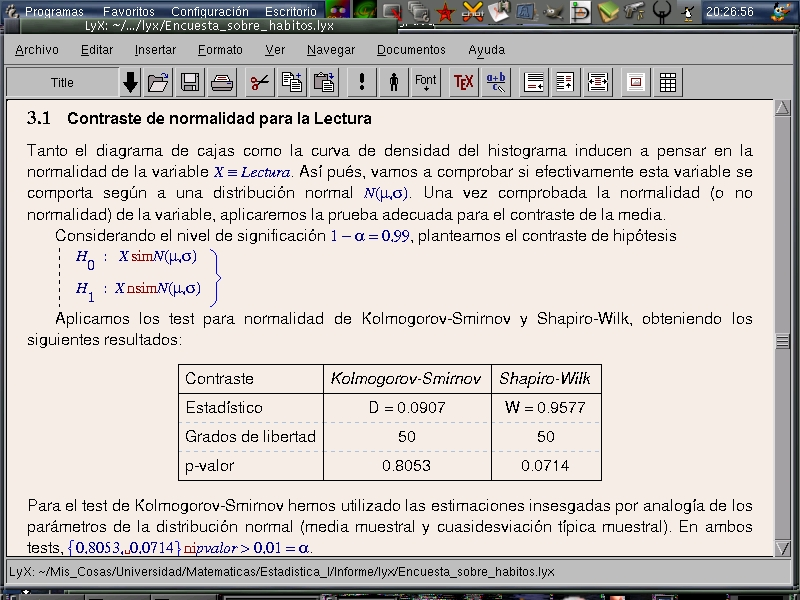
\includegraphics[width=\textwidth]{imagenes/lyx.eps}
% \caption{\LyX~ con un trabajo acad�mico sobre inferencia estad�stica}
% \end{figure}

\section{�Bienvenido a \LyX{}!}

Este fichero ha sido dise�ado para todos aquellos que nunca han o�do
hablar de \LaTeX{}, o no lo conocen muy bien. No tengas miedo, no
tendr�s que aprender \LaTeX{} para poder usar \LyX{}. Ese es, al fin
y al cabo, el punto fuerte de \LyX{}: proporcionar un interfaz casi
WYSIWIG (\emph{What You See Is What You Get}) para \LaTeX{}. Sin embargo,
hay algunas cosas que necesitar�s aprender para usar \LyX{} de forma
eficiente.

Probablemente has acabado consultando este documento porque has intentado
poner dos espacios despu�s de un punto, o tres l�neas en blanco entre
dos p�rrafos. Tras mucha frustraci�n, has comprobado que no se puede.
De hecho, descubrir�s que la mayor�a de los peque�os trucos que estabas
acostumbrado a usar con otros procesadores de texto no funcionan en
\LyX{}. La raz�n es que la mayor�a de los procesadores de texto que
has usado hasta ahora necesitaban que el usuario hiciera a mano todo
el espaciado, los cambios de tipo de letra, etc. As�, no s�lo se escrib�a
el documento, sino que adem�s se acababa realizando todo el trabajo
de formato y composici�n. \LyX{} realiza este trabajo por t� de forma
consistente, dejando que te centres en lo m�s importante: el contenido
del documento.

As� pues, ten paciencia con nosotros y sigue leyendo. Merece la pena
que leas este tema.


\subsection{Qu� \emph{es} este tema y qu� \emph{no} \emph{es}}

Antes de  que empecemos  con esta secci�n,  queremos hacer  un peque�o
apunte. El \emph{Tutorial} usa las convenciones tipogr�ficas se�aladas
en la p�gina \pageref{convenciones_tipograficas} Si has llegado a este
manual primero, ve y lee las convenciones tipogr�ficas. S�, ahora.

Una vez que ya sabes qu� significa cada tipo de letra, vamos a hablar
un poco sobre la finalidad de este \emph{Tutorial}.


\subsubsection{Para aprovechar al m�ximo el tema}

Este \emph{Tutorial} se compone de ejemplos y ejercicios. Para obtener
el m�ximo provecho de este documento, deber�as leerlo todo, tecleando
todos los peque�os detalles que te vayamos explicando (por simples
que sean) e intentando hacer todos los ejercicios para comprobar que
lo entiendes. 

% Por comodidad, puede interesarte imprimir la versi�n PostScript� de este documento.

Si est�s familiarizado con \LaTeX{}, probablemente podr�s leer el
\emph{Tutorial} m�s deprisa, ya que muchas de las ideas de \LyX{}
son realmente ideas de \LaTeX{} disfrazadas. No obstante, \LyX{} no
tiene peculiaridades%
\footnote{o dicho de manera m�s optimista, {}``caracter�sticas''%
} que tengas que aprender. Incluso aunque no te apetezca leer el resto
del \emph{Tutorial}, har�as bien en mirar la secci�n \ref{sec:latexusers},
que ha sido escrita espec�ficamente para usuarios experimentados de
\LaTeX{}.

La secci�n \ref{sec:what-is-lyx} ha quedado sin actualizar de una
versi�n anterior del \emph{Tutorial}, y es un poco general. A�n as�,
es una buena introducci�n {}``panor�mica'' a \LyX{}, as� que deber�as
echarle un vistazo para ir haci�ndote una idea sobre �l.


\subsubsection{Qu� \emph{no} vas a encontrar}

\begin{itemize}

% \item Las lecciones masticadas y dadas de comer con cuchara.

% La tendencia actual%
% \footnote{Nota de \noun{John} Weiss: \ldots{}bueno, al menos en Estados Unidos,
% donde reducimos todo al m�nimo com�n denominador\ldots{}%
% } en la literatura autodidacta inform�tica parece ser: {}``Se asume
% que el usuario tiene el coeficiente intelectual de un mosquito''.
% Nosotros no vamos a hacer eso. 

% Por otro lado, somos conscientes de que la mayor�a de los usuarios
% acuden a un manual, especialmente a un tutorial, cuando se encuentran
% perdidos. As� pues, asumiremos que t�, el usuario, \emph{no} eres
% est�pido, pero entenderemos que puedas estar un poco despistado o
% confuso.

% \item Instrucciones de c�mo usar el rat�n o el teclado.

% Si todav�a no has aprendido a usar tu ordenador no podemos ayudarte,
% est� m�s all� del alcance de estos manuales.%
% \footnote{Adem�s de que, si est�s usando \LyX{} para empezar, seguramente tienes
% m�s de medio cerebro en la cabeza.%
% }

\item Explicaci�n detallada de todas las caracter�sticas de \LyX{}.

% �Qu�? �quieres la \emph{Gu�a del Usuario} dos veces?

% Hablando en serio, 

Nuestro  objetivo  con  este  tutorial es  prepararte  para  que  s�lo
necesites  la \emph{Gu�a  del  Usuario}. Tratar  de  duplicar toda  la
informaci�n sobre las caracter�sticas de \LyX{} aqu� ser�a redundante,
demasiado largo y estar�a siempre obsoleto. Todo lo que pretendemos es
introducir las cosas; como puedes  imaginar, hay un {}``ver \emph{Gu�a
del Usuario}'' al final de cada secci�n.

\item Explicaci�n detallada de \LaTeX{}.  Para eso tienes el tema \ref{latex.tex}

% Innecesario. Si  de verdad tienes  curiosidad por aprender  algunos de
% los trucos que puedes hacer  con \LaTeX{}, siempre puedes conseguir un
% libro  espec�fico.  Hay varios  libros  buenos  sobre  el tema  en  el
% mercado. Despu�s  de todo, no  hay necesidad  de volver a  inventar la
% rueda\ldots{}

\end{itemize}

As� pues, esp�ritu intr�pido, es hora de seguir adelante. Puedes hacer
una breve excursi�n por la siguiente secci�n, o puedes continuar con
la secci�n \ref{sec:first-doc-ex}.


\subsection{�Qu� es \LyX{}?\label{sec:what-is-lyx}}


\subsubsection{Visi�n general}

Parte del reto inicial de usar \LyX{} surge del cambio en la manera
de pensar que t�, el usuario, debes hacer. En su momento, todo lo
que ten�amos para crear documentos eran m�quinas de escribir, as�
que aprendimos verdaderas artima�as para evitar sus limitaciones.
Subrayar, que es poco m�s que sobreescribir con el car�cter {}``\_'',
se convirti� en un forma de resaltar texto. Para crear una tabla,
establec�as a mano el ancho de cada columna y pon�as las tabulaciones
necesarias. Lo mismo se aplicaba para cartas y otros textos sangrados
a la derecha. Adem�s, la ruptura de palabras al final de l�nea requer�a
ser muy cuidadoso y previsor.

En otras palabras, todos hemos sido entrenados para preocuparnos por
los peque�os detalles de {}``qu� caracter va en qu� lugar''.

Como consecuencia, casi todos los procesadores de texto se basan en
esta mentalidad. Todav�a usan tabuladores para a�adir espacios en
blanco. Todav�a te tienes que preocupar de en qu� parte exacta de
la p�gina saldr� cada cosa. Resaltar texto significa cambiar el tipo
de letra, similar a cambiar la rueda de una m�quina de escribir.

Aqu� es donde \LyX{} difiere de un procesador de texto corriente.
No te tienes que preocupar de que una letra vaya en un sitio determinado.
Le dices a \LyX{} \emph{lo que est�s haciendo} y �l se preocupa de
todo lo dem�s, siguiendo un conjunto de reglas llamado estilo. Veamos
un peque�o ejemplo.

Sup�n que est�s realizando un informe. Quieres que comience con una
secci�n llamada {}``Introducci�n''. As� pues, te diriges a cualquiera
que sea el men� de tu procesador de texto que cambia el tama�o de
fuente y eliges un nuevo tama�o. Despu�s cambias tambi�n a negrita.
Seguidamente escribes: {}``1.\_Introducci�n''. Por supuesto, si
m�s tarde decides que esta secci�n pertenece a alguna otra parte del
documento, o bien insertas una nueva secci�n anterior a �sta, tienes
que cambiarle la numeraci�n a ella y a todas las posteriores, adem�s
de las correspondientes entradas en el �ndice.

En \LyX{}, te diriges a la lista situada a la derecha de todos los
botones y eliges \textsf{Secci�n}, y escribes {}``Introducci�n''.

Eso es todo. Si cortas y pegas la secci�n en otra parte, todo se renumera
autom�ticamente. Se puede hacer incluso que \LyX{} actualice cualquier
referencia a la secci�n que est� dentro del fichero.

Con el procesador de texto tradicional hay problemas de consistencia.
Cinco d�as m�s tarde, abres tu informe y comienzas la secci�n 4. Sin
embargo, has olvidado que estabas usando la letra en negrita de 18
puntos, y usas la de 16, as� que acabas escribiendo el encabezado
de la secci�n 4 con un tipo de letra distinto al que usaste para la
secci�n 1. Este problema ni siquiera existe en \LyX{}. El ordenador
se encarga de todo el tedioso trabajo de llevar la cuenta de tama�os
y fuentes, no t�. Al fin y al cabo, para eso est� hecho.

Otro ejemplo. Sup�n que est�s haciendo una lista. En otros procesadores
de texto una lista es s�lo una mera secuencia de tabuladores y saltos
de l�nea. Necesitas pensar d�nde poner la etiqueta de cada elemento
de la lista, qu� debe ser esa etiqueta, cu�ntas l�neas en blanco hay
que poner entre cada elemento, etc. Con \LyX{}, s�lo tienes dos preocupaciones:
qu� clase de lista es, y qu� vas a poner en ella. Eso es todo.

As� pues, la idea esencial detr�s de \LyX{} es especificar lo que
se est� haciendo, no c�mo hacerlo. En lugar de un procesador {}``lo
que ves es lo que obtienes'' (WYSIWIG, What You See Is What You Get),
el modelo de \LyX{} es {}``lo que ves es lo que quieres decir''
(WYSIWIM, What You See Is What You Mean).


\subsubsection{Diferencias entre \LyX{}}

He aqu� una lista de cosas que no encontrar�s en \LyX{}:

\begin{itemize}
\item La regla (para medir m�rgenes)
\item Tabuladores
\item Espacios en blanco adicionales (i.e. pulsar \textsf{Intro} o \textsf{Espacio}
dos o m�s veces)
\end{itemize}
Los tabuladores, as� como la regla (que te muestra la posici�n de
cada elemento en la p�gina), son in�tiles en \LyX{}. El programa se
preocupa de d�nde tiene que ir cada cosa, no t�. Con los espacios
en blanco adicionales ocurre lo mismo; \LyX{} los a�ade conforme son
necesarios, seg�n el contexto. Al principio puede resultar molesto
no poder escribir dos l�neas en blanco seguidas, pero cobra mucho
m�s sentido una vez que empiezas a pensar en t�rminos WYSIWYM.

Y aqu� tienes algunas cosas que presenta \LyX{} pero que no se usan
como podr�as pensar:

\begin{itemize}
\item Controles de sangrado
\item Saltos de p�gina
\item Espaciado entre l�neas (i.e. espaciado simple, doble, etc.)
\item Espacio en blanco, horizontal y vertical
\item Tipos de letra y tama�o
\item Estilo de letra (negrita, cursiva, subrayado, etc.)
\end{itemize}
Aunque aparecen en \LyX{}, no se necesitan normalmente. El programa
se preocupa de estas cosas por t�, actuando en consecuencia seg�n
lo que est�s haciendo. Diferentes partes del documento son autom�ticamente
puestas en diferente tama�o y estilo. El sangrado de cada p�rrafo
es dependiente del contexto; cada tipo de p�rrafo se sangra de manera
diferente. Los saltos de p�gina se manejan tambi�n de forma autom�tica.
En general, el espacio entre l�neas, entre palabras y entre p�rrafos
es variable, elegido por \LyX{}.%
\footnote{Se pueden ajustar todas estas caracter�sticas (s�lo el ajuste de unas
pocas requiere conocimientos de \LaTeX{}), tanto para todo el documento
como para una parte concreta. Ver Gu�a del Usuario para m�s detalles.%
}

Por �ltimo, �stas son las �reas en las que \LyX{} (y \LaTeX{}) sobrepasan
a muchos procesadores de texto:

\begin{itemize}
\item Separaci�n de palabras a final de l�nea
\item Listas de cualquier tipo
\item Matem�ticas
\item Tablas
\item Referencias cruzadas
\end{itemize}
Por supuesto, muchos procesadores de texto modernos manejan s�mbolos
matem�ticos, tablas, separaci�n de palabras a final de l�nea, e incluso
comienzan a aproximarse a las definiciones de estilo y el concepto
WYSIWYM. Sin embargo, acaban de empezar a incluir estas caracter�sticas,
mientras que \LyX{} est� construido sobre el sistema de proceso de
documentos \LaTeX{}. �ste lleva m�s de 10 a�os con ellas, y \emph{funciona}.
Todos los errores han sido subsanados hace tiempo.%
\footnote{De acuerdo, nada es perfecto, pero \LaTeX{} es lo m�s cercano a un
programa libre de errores que se puede conseguir.%
}


\subsection{�Qu� es \LaTeX{}?}

\LaTeX{} es un sistema de preparaci�n de documentos dise�ado por Leslie
Lamport en 1985.%
\footnote{La informaci�n de esta secci�n ha sido extra�da de {}``A Guide to
\LaTeXe{}'', de Helmut Kopka y Patrick Daly, documento incluido en
la bibliograf�a de la \emph{Gu�a del Usuario}.%
} Fue construido gradualmente sobre un lenguaje de composici�n de documentos
llamado \TeX{}, creado por Donald Knuth en 1984. {}``\TeX{}'' se
pronuncia como {}``blech'' en ingl�s%
\footnote{El ruido que se hace cuando se come algo con mal sabor, especialmente
los ni�os peque�os cuando no les gusta la comida. (N. del T.)%
}. Sin embargo, muchos no comprenden qu� es exactamente. \TeX{} toma
una secuencia de �rdenes de composici�n escritos en un fichero ASCII,
y los ejecuta. Es m�s complicado que una m�quina de escribir, pero
sin llegar a la especializaci�n y complejidad de una aut�ntica imprenta.
En cualquier caso, produce como salida un fichero de formato llamado
{}``independiente de dispositivo'', o \texttt{dvi} para abreviar.
El fichero \texttt{dvi} puede ser le�do depu�s por otro programa que
acepte este formato, o convertido a otros formatos, como PostScript�.

Si no tuviera m�s caracter�stica que �sta, ser�a un mero motor de
composici�n. Sin embargo, \TeX{} tambi�n permite definir macros. Aqu�
es donde comienza la acci�n.

La mayor�a de la gente que usa \TeX{} est� usando realmente un conjunto
de macros que Knuth cre� para ocultar muchos de los detalles de composici�n.
Esto es en lo que piensa la gente cuando habla de \TeX{}. Los usuarios
normales no trabajan con \TeX{} puro, un esqueleto desnudo formado
�nicamente por comandos de composici�n. S�lo aqu�llos que crean conjuntos
de macros lo hacen. Y aqu� es donde Leslie Lamport entra en nuestra
historia. �l quer�a macros que fueran m�s orientadas al usuario y
menos a la composici�n, un conjunto de comandos que sirvieran para
componer secciones, tablas o f�rmulas matem�ticas de una forma consistente
y uniforme, sin demasiadas complicaciones. As� naci� \LaTeX{}.

Ahora, de manera simult�nea al desarrollo y crecimiento de \LaTeX{},
otras personas est�n creando sus propios paquetes personalizados de
macros para \TeX{}, algunos para realizar trabajos en publicaciones
matem�ticas y cosas as�. Unos usaron \TeX{} directamente, otros comenzaron
a modificar \LaTeX{}. Para tratar de unificar este l�o, un equipo
de expertos en \LaTeX{} (incluyendo a Lamport, por supuesto), empezaron
a trabajar en \LaTeXe{}, la versi�n actual del programa, a finales
de los ochenta. Esta nueva versi�n posee comandos que proporcionan
una interfaz m�s f�cil para la creaci�n de macros, ayuda para usar
las nuevas fuentes, y m�s mejoras. De hecho, \LaTeX{} es en s� mismo
un vasto lenguaje por derecho propio. Usuarios de todo el mundo han
estado creando sus propios a�adidos para \LaTeX{}, adem�s de los est�ndar.

Existen dos formas de extender \LaTeX{}: las clases y los estilos.
Una \emph{clase} es un conjunto de macros de \LaTeX{} (y de \TeX{})
que describen un nuevo tipo de documento, como un libro o un art�culo.
Hay clases para transparencias, para publicaciones de f�sica y matem�ticas\ldots{}
�algunas universidades tienen incluso una clase para su propio formato
de tesis! Un \emph{estilo,} a diferencia de una clase, no define un
nuevo tipo de documento, sino un nuevo tipo de \emph{comportamiento},
que puede ser utilizado por cualquier documento. Por ejemplo, \LyX{}
controla los m�rgenes de p�gina y el espaciado entre l�neas usando
dos ficheros de estilo diferentes de \LaTeX{}, dise�ados para este
fin. Hay ficheros de estilo para gran cantidad de cosas: imprimir
etiquetas o sobres, cambiar el sangrado normal del texto, a�adir nuevos
tipos de letra, manipular gr�ficos, dise�ar elaborados encabezados
de p�gina, personalizar bibliograf�as, alterar la posici�n y apariencia
de notas a pie de p�gina, tablas y figuras, personalizar listas, etc,
etc.

Aqu� tienes un resumen:

\begin{lyxlist}{00.00.0000}
\item [\TeX{}:]Lenguaje de composici�n con capacidad para uso y creaci�n
de macros.
\item [\LaTeX{}:]Paquete de macros construido sobre \TeX{}\@.
\item [clases:]Descripciones de un tipo de documento, usando \LaTeX{}\@.
\item [estilos:]Alteran alg�n aspecto del comportamiento normal de \LaTeX{}.
\item [\LyX{}:]Procesador de texto visual, WYSIWYM, que usa toda la potencia
de \LaTeX{} para realizar el trabajo de composici�n.
\end{lyxlist}
La idea de esta secci�n ha sido tratar de explicarte \emph{por qu�}
\LyX{} funciona de manera diferente a otros procesadores de texto.
La raz�n es simple: usa \LaTeX{} como motor de composici�n. Como este
�ltimo, se centra en el contexto de tu escritura \emph{(lo que} est�s
escribiendo). El ordenador se encarga entonces de c�mo debe aparecer.

Ah, una cosa m�s. \LaTeX{} se pronuncia como \TeX{}. Rima con {}``hey
blech''.%
\footnote{Estos detalles de pronunciaci�n no son relevantes para hispanohablantes.
\TeX{}, \LaTeX{} y \LyX{} tienen pronunciaci�n directa en espa�ol
(N. del T.)%
} Lamport, sin embargo, dice en su libro que {}``\emph{lay}-tecks
tambi�n es posible''. Por otro lado, {}``\LyX{}'' se pronuncia
como {}``licks'', {}``lucks'' o {}``looks'', dependiendo de
la pronunciaci�n de cada pa�s\ldots{}


% \chapter{Empezando con \LyX{}}


\section{Tu primer documento \LyX{}}

\label{sec:first-doc-ex} Muy bien\@. Ya est�s listo para empezar
a escribir. Sin embargo, antes de que lo hagas hay un par de cosas
que debemos decir, y que esperamos har�n el \emph{Tutorial} m�s instructivo,
�til y divertido.

Como hay mucha informaci�n que no te vamos a dar aqu�, lo primero
que tienes que hacer es encontrar los otros ficheros de ayuda. Afortunadamente,
esto es muy simple. Arranca \LyX{}. Elige la \emph{Gu�a del Usuario}
en el men� \textsf{A}\textsf{\underbar{y}}\textsf{uda}. Tambi�n puedes
cargar el \emph{Tutorial} (si es que no lo est�s leyendo ya desde
ah�). De esta forma, puedes leerlos mientras escribes tu propio fichero%
\footnote{Tambi�n pueden servir como buenos ejemplos de uso de las caracter�sticas
de \LyX{}.%
}. Ten en cuenta que, una vez que tienes m�s de un documento abierto,
puedes usar el men� \textsf{\underbar{D}}\textsf{ocumentos} para alternar
entre ellos. El \emph{Tutorial} no va a cubrir en detalle aquellos
temas que sean tratados en otros manuales de \LyX{}. Esto puede complicarte
la vida al principio, pero evita que el \emph{Tutorial} se haga muy
extenso. Te acostumbrar� tambi�n a usar los dem�s manuales, lo cual
---a largo plazo--- te ahorar� mucho tiempo.

En este \emph{Tutorial}, vamos a asumir que tienes instalada una versi�n
de \LyX{} funcionando perfectamente, as� como \LaTeX{}, \texttt{xdvi}
o cualquier otro visor de ficheros dvi, \texttt{dvips} o alguna otra
forma de convertir documentos \texttt{dvi} a PostScript�, y una impresora.
Esto es asumir mucho. Si alguna de estas condiciones no se cumple,
t� mismo deber�s configurar aquello que falte (o bien tu administrador
del sistema). Encontrar�s informaci�n sobre configuraci�n en otros
manuales.

Finalmente, hemos preparado un fichero para que practiques tus habilidades
con \LyX{} en �l. Se llama \texttt{es\_ejemplo\_sin\_lyx.lyx}. Imagina
que fue escrito por alguien que no conoce ninguna de las magn�ficas
caracter�sticas de \LyX{}. Conforme vayas aprendiendo nuevas funciones
te iremos sugiriendo que corrijas las partes correspondientes del
fichero \texttt{es\_ejemplo\_sin\_lyx.lyx}. Adem�s, contiene {}``sutiles''
trucos sobre c�mo arreglar las cosas%
\footnote{Los trucos se encuentran en {}``notas'' amarillas. Puedes leerlas
pulsado con el rat�n sobre ellas.%
}. Si quieres hacer trampa (o comprobar lo que has hecho), hay tambi�n
un fichero llamado \texttt{es\_ejemplo\_con\_lyx.lyx} que contiene
el mismo texto, pero escrito por un experto en \LyX{}.

Los ficheros de ejemplo se pueden encontrar en el directorio \texttt{examples/},
que puedes conseguir seleccionando \textsf{\underbar{A}}\textsf{rchivo\lyxarrow{}}\textsf{\underbar{A}}\textsf{brir}
y pulsando el bot�n \textsf{Ejemplos}. Abre el documento sin procesar
(\texttt{es\_ejemplo\_sin\_lyx.lyx}), y usa el men� \textsf{\underbar{A}}\textsf{rchivo\lyxarrow{}Guardar}
\textsf{\underbar{C}}\textsf{omo} para guardar una copia en tu propio
directorio para que puedas trabajar con �l. Conforme vayas arreglando
el documento, comprueba c�mo los cambios afectan a la salida dvi (\textsf{\underbar{A}}\textsf{rchivo\lyxarrow{}Ver
dvi}).

Por cierto, el directorio \texttt{examples/} contiene muchos otros
ficheros de ejemplo que te ense�ar�n c�mo hacer con \LyX{} algunas
cosas bastante elaboradas. Son especialmente �tiles para mostrar aquello
que no cabr�a en la documentaci�n (por su extensi�n u otras razones).
Despu�s de leer el \emph{Tutorial}, o cuando est�s confundido a la
hora de hacer algo complicado con \LyX{}, echa un ojeada a estos ficheros.


\subsection{Escribir, ver e imprimir}

\begin{itemize}
\item Abre un fichero nuevo con \textsf{\underbar{A}}\textsf{rchivo\lyxarrow{}}\textsf{\underbar{N}}\textsf{uevo}
\item Escribe una frase: \texttt{�Este es mi primer documento LyX!}%
\footnote{De acuerdo. Realmente puedes escribir lo que quieras. No importa.
Nos disculpamos por la estupidez de esta frase, y de todas las que
te vamos a pedir que escribas de aqu� en adelante.%
}
\item Guarda el documento con \textsf{\underbar{A}}\textsf{rchivo\lyxarrow{}Guardar}
\textsf{\underbar{C}}\textsf{omo\@.}
\item Ejecuta \LaTeX{} para crear un fichero \texttt{dvi}, con \textsf{\underbar{A}}\textsf{rchivo\lyxarrow{}Ver
dvi}\@. Puedes ver que se imprimen algunas l�neas en la ventana desde
la que has ejecutado el comando lyx. Se trata de mensajes de \LaTeX{},
que por ahora puedes ignorar. \LyX{} lanzar� el programa \texttt{xdvi}
(o alg�n otro visualizador de ficheros \texttt{dvi}), que abrir� una
nueva ventana mostr�ndote el aspecto de tu documento cuando est� impreso.%
\footnote{Puedes ahorrar tiempo dejando que \texttt{xdvi} se ejecute en segundo
plano. De esta forma, puedes usar \textsf{\underbar{A}}\textsf{rchivo\lyxarrow\underbar{A}ctualizar
dvi} y simplemente pulsar sobre la ventana de \texttt{xdvi} (o restaurarla)
cuando \LaTeX{} termine de ejecutarse.%
}
\item Imprime con \textsf{}\textsf{\underbar{A}}\textsf{rchivo\lyxarrow{}Im}\textsf{\underbar{p}}\textsf{rimir}
y pulsa \textsf{OK\@.}
\end{itemize}
�Enhorabuena! Has escrito e impreso tu primer documento \LyX{}. Todo
lo dem�s son detalles, a cubrir por el resto del \emph{Tutorial},
la \emph{Gu�a del Usuario} y el \emph{Manual de Referencia}.


\subsection{Operaciones sencillas}

Por supuesto, \LyX{} puede realizar la mayor�a de las cosas a las
que est�s acostumbrado con tu procesador de texto. Separar� las palabras
y justificar� los p�rrafos autom�ticamente. Basta que accedas a un
par de men�s%
\footnote{Si eres como tantos usuarios de \noun{unix}, lo habr�s hecho ya
mucho antes de empezar a leer el \emph{Tutorial}.%
} para que veas c�mo la mayor parte de los comandos simples (i.e.,
\textsf{\underbar{A}}\textsf{rchivo\lyxarrow{}Salir,} \textsf{\underbar{E}}\textsf{dici�n\lyxarrow{}P}\textsf{\underbar{e}}\textsf{gar,}
\textsf{\underbar{A}}\textsf{rchivo\lyxarrow{}Im}\textsf{\underbar{p}}\textsf{rimir)}
tienen los nombres que esperas que tengan, est�n en el men� donde
esperas que est�n, y funcionan tal y como esperas que funcionen. A
continuaci�n tienes una descripci�n r�pida de c�mo realizar algunas
acciones sencillas.

\begin{description}
\item [Deshacer]\LyX{} tiene capacidad para {}``deshacer infinitas veces'',
lo que significa que puedes deshacer todo lo que lo que hayas hecho
desde que empezaste la sesi�n actual, aplicando una y otra vez \textsf{\underbar{E}}\textsf{dici�n\lyxarrow{}Deshacer}.
Si deshaces demasiado, elige simplemente \textsf{\underbar{E}}\textsf{dici�n\lyxarrow{}}\textsf{\underbar{R}}\textsf{ehacer}
para recuperar los cambios. Actualmente, el comando deshacer est�
\emph{limitado a 100 pasos.} Tampoco funciona \emph{para todo} (por
ejemplo, en los cambios de formato de documento).
\item [Cortar/Pegar/Copiar]Utiliza \textsf{\underbar{E}}\textsf{dici�n\lyxarrow{}}\textsf{\underbar{C}}\textsf{ortar},
\textsf{\underbar{E}}\textsf{dici�n\lyxarrow{}}\textsf{\underbar{P}}\textsf{egar},
y \textsf{\underbar{E}}\textsf{dici�n\lyxarrow{}C}\textsf{\underbar{o}}\textsf{piar}
para cortar, pegar y copiar. O pega autom�ticamente el texto seleccionado
con el bot�n central del rat�n.
\item [Buscar/Reemplazar]Utiliza \textsf{\underbar{E}}\textsf{dici�n\lyxarrow{}}\textsf{\underbar{B}}\textsf{uscar~y~Reemplazar}
para realizar una b�squeda sensible a las may�sculas. En el men� que
se despliega a tal efecto, puedes desplazarte hacia delante y hacia
atr�s en la b�squeda mediante las flechas, y reemplazar aquellas palabras
que hayas encontrado con el bot�n \textsf{\underbar{R}}\textsf{eemplazar}.%
\footnote{Cierra la ventana cuando hayas acabado, o d�jala abierta si lo encuentras
m�s conveniente. La mayor�a de los men�s contextuales de \LyX{} (incluyendo
los de \textsf{\underbar{B}}\textsf{uscar~y~Reemplazar, �ndice~Gener}\textsf{\underbar{a}}\textsf{l}
y \textsf{\underbar{F}}ormato, as� como los de matem�ticas) son ventanas
que pueden ser apartadas, en vez de cerradas. Unos pocos men�s como
\textsf{\underbar{A}}\textsf{rchivo\lyxarrow{}}\textsf{\underbar{A}}\textsf{brir},
no te dejar�n escribir nada en la ventana principal hasta que los
cierres. Aseg�rate de que el foco est� en la ventana correcta cuando
est�s tratando escribir en la ventana principal de \LyX{} o introduciendo
un comando en alguna ventana de di�logo.%
}
\item [Formato~de~caracteres]Puedes \emph{resaltar} texto (lo que normalmente
significa poner los caracteres en cursiva), ponerlo en \textbf{negrita},
o en \noun{Estilo Nombre} (habitualmente en min�sculas, para nombres
propios de personas) desde los botones interruptor en el men� \textsf{\underbar{F}}\textsf{ormato}.
\item [Barra~de~herramientas]Sus botones (justo debajo de los men�s)
te permiten realizar las funciones m�s usuales, como \textsf{Pegar}
e \textsf{Imprimir}. Si mantienes el cursor del rat�n sobre alguno
de los botones de la barra, una peque�a nota amarilla te informar�
sobre la funci�n concreta del bot�n.
\item [\emph{Minibuffer}]La franja gris en la parte de abajo de la ventana
de \LyX{} recibe el nombre de \emph{minibuffer}. Se encarga de mostrarte
toda clase de informaci�n �til. Por ejemplo, cuando guardas, te dice
el nombre del fichero que acabas de guardar. Tambi�n muestra algunos
mensajes de error. Observa que puedes escribir en �l. Esto te ofrece
una gran funcionalidad, incluyendo la posibilidad de estropear el
documento. En otras palabras, no escribas en el \emph{minibuffer}
a menos que sepas lo que est�s haciendo.
\end{description}
Por supuesto, todav�a no has escrito suficiente para encontrar �tiles
todas estas funciones. Conforme vayas escribiendo m�s, prueba a deshacer,
copiar, pegar, etc.


\subsection{WYSIWYM: el espacio en blanco en \LyX{}}

\label{sec:whitespace}Una de las cosas m�s dif�ciles para los nuevos
usuarios es acostumbrarse a la forma en que \LyX{} maneja el espacio
en blanco. Por mucho que pulses \textsf{Retorno de carro}, s�lo conseguir�s
una �nica l�nea en blanco. Por mucho que pulses la \textsf{Barra espaciadora},
s�lo conseguir�s un �nico espacio en blanco. En una l�nea vac�a \LyX{}
no te dejar� poner ni siquiera un espacio. El \textsf{Tabulador} no
te adelantar� ning�n espacio, �de hecho no hay tabulaci�n! Tampoco
hay ninguna regla en la parte superior de la p�gina que te permita
definir tabulaciones o m�rgenes.

Muchos procesadores de texto comerciales est�n basados en el principio
WYSIWYG: {}``lo que ves es lo que obtienes''. \LyX{}, por el contrario,
est� basado en el principio {}``lo que ves es lo que quieres decir''.
Escribes lo que quieres decir, y \LyX{} se preocupar� de la composici�n
por t� para que el resultado final quede bien. Un \textsf{Retorno
de carro} gramaticalmente separa p�rrafos, y de la misma forma un
\textsf{espacio} separa palabras, as� que no hay ninguna raz�n para
poner varios seguidos; un \textsf{Tabulador} no tiene funci�n gramatical
alguna, as� que \LyX{} no los usa. Con \LyX{} emplear�s m�s tiempo
en el contenido del documento, y menos en la forma. Ver Secci�n \ref{sec:what-is-lyx}
para m�s informaci�n sobre el concepto WYSIWYM.

\LyX{} tiene (muchas) formas de ajustar al detalle el formato del
documento. Despu�s de todo, podr�a no imprimirse exactamente lo que
quer�as decir. La \emph{Gu�a del Usuario} contiene informaci�n sobre
eso. Incluye espaciado vertical y horizontal ---mucho m�s potentes
y vers�tiles que m�ltiples espacios o l�neas en blanco--- y formas
de cambiar tama�o y estilo de letra y alineaci�n de p�rrafos a mano.
La idea es que puedas escribir todo el documento concentr�ndote en
el contenido, y solamente te preocupes de ajustar los detalles al
final. Con los procesadores de texto convencionales, el formato te
distrae continuamente.


\section{Entornos}

Las diferentes partes de un documento tienen prop�sitos diferentes;
llamaremos a estas partes \emph{entornos}. La mayor parte del documento
est� formada por texto normal. Los t�tulos de secci�n (cap�tulos,
subsecciones, etc.) permiten al lector saber que se va a tratar un
nuevo concepto o idea. Ciertos tipos de documentos tienen entornos
especiales. Un art�tculo de peri�dico tendr� un resumen y un t�tulo.
Una carta no tendr� nada de eso, pero probablemente contendr� un entorno
para la direcci�n del remitente.

Los entornos son una parte importante en la filosof�a {}``lo que
ves es lo que quieres decir'' de \LyX{}. Un entorno dado puede requerir
un cierto estilo o tama�o de letra, sangrado, espaciado y otras caracter�sticas.
Este problema se agrava cuando el formato exacto de un entorno puede
cambiar: un peri�dico puede usar letra en negrita, de 18 puntos con
p�rrafos centrados para los t�tulos, mientras que otros pueden usar
p�rrafos justificados con letra cursiva de 15 puntos; idiomas distintos
pueden tener diferentes convenios para el sangrado; y los formatos
de bibliograf�a pueden variar ampliamente. \LyX{} te evita tener que
aprender todos los diferentes estilos de formato.

La caja de \textsf{Entorno} se sit�a al final a la izquierda en la
barra de herramientas (justo debajo del men� \textsf{\underbar{A}}\textsf{rchivo}).
Indica qu� entorno est�s usando en cada momento. Mientras escrib�as
tu primer documento, dec�a {}``Standard'' (normal), que es el entorno
por defecto para texto. Ahora vas a usar varios entornos en el nuevo
documento para que puedas ver c�mo funcionan. Lo har�s con el men�
\textsf{Entorno,} que puedes abrir pulsando sobre el icono con {}``la
flecha hacia abajo'' justo a la derecha de la caja de \textsf{Entorno.}


\subsection{Secciones y subsecciones}

Escribe la palabra \texttt{Introducci�n} en la primera l�nea de tu
fichero \LyX{}, y elige \textsf{Section} (secci�n) en el men� de entorno%
\footnote{No tienes que seleccionar la l�nea. Si no hay nada seleccionado, \LyX{}
cambia el p�rrafo en el que est�s escribiendo ahora al entorno elegido.
Alternativamente, puedes cambiar varios p�rrafos seleccion�ndolos
antes de elegir el nuevo entorno.%
}. \LyX{} numera la secci�n como {}``1'' y escribe el encabezado
(t�tulo ) en un tipo de letra mayor (por supuesto, el encabezado aparecer�
de esta forma en el fichero \texttt{dvi} y en el documento impreso).
Ahora pulsa \textsf{Retorno de carro.} Observa que la caja de entorno
cambia de {}``Section'' a {}``Standard''. Se asume que los t�tulos
de secci�n, como muchos entornos, terminan cuando introduces un \textsf{Retorno
de carro}%
\footnote{Ver \emph{Gu�a del Usuario} para poder escribir t�tulos de m�s de
una l�nea. Desde luego, el entorno \textsf{Standard} puede continuar
a lo largo de varios p�rrafos. Los entornos de listas (ver m�s adelante)
tampoco terminan con \textsf{Retorno de carro.} Siempre puedes saber
el entorno en el que est�s mirando la caja de \textsf{Entorno.}%
}\textsf{.} Escribe la introducci�n del documento:

\begin{verbatim}
Esto es una introducci�n a mi primer documento LyX.
\end{verbatim}

Pulsa \textsf{Retorno de carro} otra vez, y elige de nuevo \textsf{Section}
en el men� entorno. \LyX{} escribe un {}``2'' y espera que intoduzcas
un t�tulo. Escribe \texttt{M�s cosas}, y ver�s que de nuevo lo establece
como t�tulo de secci�n.

La cosa mejora. Ve al final de la secci�n 1 otra vez (tras {}``mi
primer documento \LyX{}''), pulsa \textsf{Retorno de carro}, y selecciona
\textsf{Section} en el men� \textsf{Entorno}. Una vez m�s, \LyX{}
escribe {}``2'' y espera a que introduzcas un t�tulo. Escribe \texttt{Acerca
de este documento}. La secci�n {}``M�s cosas'', que antes era la
secci�n 2, �ha sido autom�ticamente renumerada a secci�n 3! De una
forma verdaderamente WYSIWYM, s�lo necesitas identificar los t�tulos
de las distintas partes de que se compone el texto, y \LyX{} se encarga
de la numeraci�n de secciones y su formato.

Pulsa \textsf{Retorno de carro} para volver al entorno \textsf{Standard}
y escribe las siguientes cinco l�neas:

\begin{verbatim}
Secciones y subsecciones se describen m�s adelante.
Descripci�n de secci�n
Las secciones son mayores que las subsecciones.
Descripci�n de subsecci�n
Las subsecciones son menores que las secciones.
\end{verbatim}

Col�cate en la segunda l�nea y elige \textsf{Subsection} (subsecci�n)
en el men� \textsf{Entorno}. \LyX{} numera la secci�n como {}``2.1'',
y la escribe con un tama�o de letra mayor que el de texto regular
pero menor que el de un t�tulo de secci�n. Cambia tambi�n el entorno
de la cuarta l�nea a \textsf{Subsection}. Como probablemente esperabas,
\LyX{} la numera autom�ticamente como secci�n {}``2.2''. Si pones
una secci�n m�s antes de la secci�n 2, �sta ser� renumerada como secci�n
3, y sus subsecciones corespondientes como {}``3.1'' y {}``3.2''.

Niveles m�s profundos de secci�n son la subsubsecci�n (\textsf{Subsubsection}),
el p�rrafo (\textsf{Paragraph}), y el subp�rrafo (\textsf{Subparagraph}).
Dejaremos que juegues t� mismo con ellos. Notar�s que los t�tulos
de p�rrafo y de subp�rrafo no est�n numerados por defecto, y que los
subp�rrafos est�n sangrados; ver \emph{Gu�a del Usuario} para cambiar
esto. Los encabezados de cap�tulo (\textsf{Chapter}) son realmente
el nivel m�s alto de la jerarqu�a, por encima de las secciones, pero
solamente se pueden utilizar en ciertos tipos (clases) de documentos
(ver Secci�n \ref{sec:textclasses}). 

Finalmente, puede que quieras usar secciones y subsecciones sin numerar.
Existen entornos para esto tambi�n. Si cambias uno de los encabezados
de secci�n al entorno \textsf{Section{*}} (puede que tengas que bajar
en el men� \textsf{Entorno} para encontralo), \LyX{} usar� el mismo
tama�o de letra que en las secciones normales, pero no la numerar�.
Tambi�n est�n los entornos {}``no numerados'' correspondientes a
\textsf{Subsection} y \textsf{Subsubsection}. Intenta cambiar alguna
de tus secciones o subsecciones a entornos no numerados, y comprueba
c�mo los dem�s n�meros de secci�n se actualizan.

\textbf{Ejercicio}: Arregla los encabezados de secci�n y subsecci�n
del fichero \texttt{es\_ejemplo\_sin\_lyx.lyx}. 


\subsection{Listas y sublistas}

\LyX{} tiene diferentes entornos para componer listas. Los variados
entornos de listas te evitan tener que pulsar el \textsf{Tabulador}
un mill�n de veces cuando est�s escribiendo un esquema, o de renumerar
toda la lista cuando quieres a�adir un nuevo punto en mitad de ella.
As� puedes concentrarte en el contenido de la lista%
\footnote{S�, estamos recalcando una y otra vez este punto a lo largo de todo
el \emph{Tutorial}. Pero \emph{es} la principal filosof�a de \LyX{},
as� que por favor, disc�lpanos.%
}. Distintos tipos de documentos requieren, l�gicamente, entornos de
lista diferentes:

\begin{itemize}
\item Una exposici�n de diapositivas podr�a usar las listas simples (etiquetadas
con bolos) del entorno \textsf{Itemize} para describir los diferentes
puntos.
\item Un esquema usar�a las listas numeradas (y sublistas etiquetadas con
letras) del entorno \textsf{Enumerate} (enumeraci�n). 
\item Un documento que describa varios paquetes de software usar�a el entorno
\textsf{Description} (descripci�n), en el que cada elemento de la
lista comienza con una palabra en negrita. 
\item El entorno \textsf{List} (que no existe en \LaTeX{}) es ligeramente
diferente al entorno \textsf{Description}.
\end{itemize}
Vamos a escribir una lista de razones por las que \LyX{} es mejor
que otros procesadores de texto. En cualquier parte de tu documento
escribe:

\begin{verbatim}
LyX es mejor que otros procesadores de texto porque:
\end{verbatim}

y pulsa \textsf{Retorno de carro}. Ahora elige \textsf{Itemize} en
el men� de \textsf{Entorno}. \LyX{} pondr� un bolo (realmente un asterisco,
que se convertir� en un c�rculo en la salida final) en la l�nea. Introduce
tus razones:

\begin{verbatim}
LyX realiza la composici�n por t�.
Las matem�ticas son WYSIWYG
Las listas son muy f�ciles de crear
\end{verbatim}

Los entornos de listas, al contrario que los encabezados, no terminan
cuando introduces un \textsf{Retorno de carro}. En vez de eso, \LyX{}
asume que vas a introducir el siguiente elemento de la lista. La anterior
resultar� ser una lista de tres elementos. Si deseas m�s de un p�rrafo
en un solo \emph{elemento} de la lista, una forma de conseguirlo es
mediante un \textsf{Retorno de carro protegido}, pulsando \textsf{C-Retorno
de carro}. Para salir de la lista tienes que volver a seleccionar
el entorno \textsf{Standard} (o usar la combinaci�n de teclas \textsf{M-p~s}).

Has conseguido una bonita lista simple. Puedes ejecutar \LaTeX{} para
ver c�mo aparece en la salida impresa. Pero, �y si quer�as numerar
las razones? Bien, simplemente selecciona toda la lista%
\footnote{\LyX{} no te dejar� seleccionar el primer bolo a menos que selecciones
el p�rrafo anterior a la lista, que probablemente no es lo que quieres
hacer. De forma similar, no puedes seleccionar el n�mero en el t�tulo
de una secci�n. No te preocupes de eso.%
} y elige el entorno \textsf{Enumerate} en el men�. �Incre�ble! Como
ya dijimos, si a�ades o borras un elemento de la lista, \LyX{} arregla
la numeraci�n.

Mientras la lista est� selecionada, puedes cambiar a los otros dos
entornos, \textsf{Description} y \textsf{List}, para ver c�mo son.
Para ambos, cada elemento de la lista est� compuesto por un t�rmino,
que es la primera palabra del elemento, seguido de una definici�n,
que es el resto del p�rrafo (hasta que pulses \textsf{Retorno de carro}).
El t�rmino se escribe en negrita (\textsf{Description}) o separado
por un {}``Tabulador''%
\footnote{Pero un tabulador de composici�n, que cambiar� para ajustarse al tama�o
del mayor t�rmino de la lista, no un r�gido, inmutable y pat�tico
\textsf{Tabulador} de m�quina de escribir.%
}(\textsf{List}) del resto del p�rrafo. Si quieres m�s de una palabra
en el t�rmino, separa las palabras con \textsf{Espacios~protegidos},
que se obtienen al pulsar \textsf{C-Espacio} y aparecen como peque�as
{}``ues'' rosas.

\textbf{Ejercicio}: Escribe correctamente la lista en el fichero \texttt{es\_ejemplo\_sin\_lyx.lyx}

Puedes anidar listas unas dentro de otras en toda clase de formas
interesantes. Un ejemplo ser�a escribir esquemas. Las listas simples
y numeradas tendr�n diferentes tipos de bolos y diferente numeraci�n
en las sublistas. Ver \emph{Gu�a del Usuario} para los detalles de
los distintos tipos de listas, as� como ejemplos de c�mo usar \emph{mucho}
anidamiento.


\subsection{M�s entornos: estrofas, citas y otros}

Hay dos entornos para separar las citas del texto que las rodea: \textsf{Quote}
para citas cortas y \textsf{Quotation} para las m�s largas. El c�digo
de ordenador (el entorno \textsf{\LyX{}-Code}, usado tambi�n en este
\emph{Tutorial} para ejemplos largos) se escribe en letra de \texttt{m�quna
de escribir}; este entorno es el �nico sitio en \LyX{} donde se permite
usar varios espacios seguidos para permitir el sangrado del c�digo.
Puedes incluso escribir poes�a mediante el entorno \textsf{Verse} (estrofa), usando \textsf{Retornos
de carro} para separar los versos, y \textsf{C-Retorno de carro} para
separar l�neas dentro de un verso. Ver Gu�a del Usuario para una descripci�n
m�s completa de todos los entornos disponibles en \LyX{}.

\textbf{Ejercicio}: Usa los entornos \textsf{Quote, \LyX{}-Code,}
y \textsf{Verse} donde corresponda en el fichero \texttt{es\_ejemplo\_sin\_lyx.lyx}


\section{Escribiendo documentos}

Esperamos que el cap�tulo anterior te haya servido para acostumbrarte
a esribir con \LyX{}. Te hemos presentado las operaciones b�sicas
de edici�n, as� como el potente m�todo de escribir con entornos. Sin
embargo, la mayor�a de la gente que usa \LyX{} querr� escribir documentos:
peri�dicos, art�culos, libros, manuales o cartas. Este cap�tulo pretende
que pases de escribir simple texto a escribir un documento completo.
Te presentar� las clases de texto, que te permiten crear distintos
tipos de documentos, y te describir� muchas caracter�sticas nuevas
que convierten texto en un documento, como t�tulos, notas a pie de
p�gina, referencias cruzadas, bibliograf�as e �ndices.


\subsection{Clases de texto y modelos}

\label{sec:textclasses}Diferentes tipos de documentos deben componerse
de forma diferente. Por ejemplo, normalmente los libros se imprimen
a doble cara, mientras que los art�culos se imprimen a simple. Adem�s,
muchos documentos contienen entornos especiales: las cartas tienen
entornos (como la direcci�n del remitente o la firma) que no tienen
sentido en un libro o un art�culo. Las \emph{clases de texto} de \LyX{}%
\footnote{Para usuarios de \LaTeX{}: equivalente a las clases de documento de
\LaTeX{} (\emph{documentclass}).%
} se encargan de estas grandes diferencias entre cada tipo de documento.
Este Tutorial, por ejemplo, se ha escrito con la clase de texto \textsf{Book}
(libro). Estas clases son otro de los grandes pilares de la filosof�a
WYSIWYM; le dicen a \LyX{} c�mo tiene que componer el documento, as�
que t� no necesitas saberlo.

Tu documento se est� escribiendo seguramente con la clase \textsf{Article}
(art�culo)%
\footnote{Normalmente el art�culo es la clase de texto por defecto, aunque puedes
establecerla en tu fichero de configuraci�n \texttt{lyxrc}.%
}. Prueba a cambiar a otras clases (usa el men� \textsf{\underbar{C}}\textsf{lase}
dentro de \textsf{\underbar{F}}\textsf{ormato\lyxarrow{}}\textsf{\underbar{D}}\textsf{ocumento})
para ver c�mo se compone cada una de ellas. Si la cambias a \textsf{Book}
y miras en el men� \textsf{Entorno}, ver�s que la mayor�a de entornos
permitidos son los mismos. Sin embargo, ahora puedes utilizar el entorno
\textsf{Chapter} (cap�tulo). Si alguna vez no est�s seguro de cu�les
tienes disponibles en una clase de texto dada, s�lo tienes que consultar
el men� \textsf{Entorno}.

El tama�o de letra, la impresi�n a una o dos columnas, o los encabezados
de p�gina son s�lo algunas de las cosas en las que difiere el formato
de composici�n de los distintos peri�dicos. Conforme la Era Digital
ha ido madurando, �stos han empezado a aceptar presentaciones electr�nicas,
creando {}``ficheros de estilo'' \LaTeX{} para que los autores puedan
enviar sus art�culos correctamente maquetados. \LyX{} tambi�n est�
preparado para esto. As� por ejemplo, ofrece soporte para composici�n
(y entornos adicionales) para los peri�dicos de la Sociedad Americana
de Matem�ticas mediante la clase de texto \textsf{Article~(AMS).}

A continuaci�n te damos una breve referencia r�pida de algunas clases
de texto. Como siempre, dir�gete a la \emph{Gu�a del Usuario} para
m�s detalles.

\vspace{0.3cm}
\begin{center}\begin{tabular}{|c|c|}
\hline 
Nombre&
Comentarios\tabularnewline
\hline
\hline 
article&
art�culo --- simple cara, sin cap�tulos\tabularnewline
\hline 
article (AMS)&
formato y entornos de la Sociedad Americana de Matem�ticas\tabularnewline
\hline 
report&
informe --- m�s extenso que el art�culo, doble cara\tabularnewline
\hline 
book&
libro --- informe + portada y contraportada\tabularnewline
\hline
slides&
transparencias (incluyendo Foil\TeX{})\tabularnewline
\hline
letter&
carta --- entornos adicionales para la direcci�n, la firma\ldots{}\tabularnewline
\hline
\end{tabular}\end{center}
\vspace{0.3cm}


\subsection{Modelos: escribir una carta}

Una de las clases de texto m�s populares es la carta. Una forma de
escribir una carta ser�a abrir un \textsf{\underbar{N}}\textsf{uevo}
fichero, y elegir \textsf{Letter} en el men� \textsf{\underbar{C}}\textsf{lase}
dentro de \textsf{\underbar{F}}\textsf{ormato\lyxarrow{}}\textsf{\underbar{D}}\textsf{ocumento}.
Aunque esta es la manera m�s obvia de hacerlo, supone trabajo de m�s.
Cada vez que escribes una carta de negocios pones tu direcci�n, la
del destinatario, el cuerpo, la firma, etc. Por tanto, \LyX{} ofrece
un \emph{modelo} para cartas, que contiene un ejemplo de carta; una
vez que tienes el modelo, s�lo tienes que sustituir un par de cosas
cada vez que quieras escribir una nueva carta.

Abre un archivo nuevo con \textsf{\underbar{A}}\textsf{rchivo\lyxarrow{}Nuevo~basado~en~Modelo}.
Tras decidir un nombre para el nuevo fichero, elige \texttt{latex\_letter.lyx}
en el men� \textsf{Seleccionar~Modelo}. Guarda e imprime el fichero
para ver c�mo se componen los distintos entornos.

Si te fijas en el men� \textsf{Entorno}, ver�s algunos entornos, como
\textsf{My~Address} (direcci�n del remitente), que no est�n disponibles
en otras clases. Otros, como \textsf{Quote} y \textsf{Description},
son familiares. Puedes jugar con ellos para ver c�mo funcionan. Comprobar�s,
por ejemplo, que en el entorno \textsf{Signature} (firma) la palabra
{}``Signature:{}`` en rojo antecede al texto de la firma. Esta palabra
no se muestra en la verdadera carta, como podr�s ver si imprimes el
fichero. S�lo est� ah� para que sepas d�nde va la firma. Ten en cuenta
tambi�n que no importa d�nde est� situada la l�nea \textsf{Signature}.
Recuerda que \LyX{} es WYSIWYM, as� que puedes poner el entorno \textsf{Signature}
en el lugar que quieras, �l sabe que en la salida impresa la firma
debe ir al final.

Un modelo es simplemente un fichero de \LyX{}. Esto quiere decir que
puedes completarlo con tu direcci�n y tu firma y guardarlo como un
nuevo modelo. A partir de ahora, siempre que quieras escribir una
carta ahorrar�s tiempo usando tu nueva plantilla. Probablemente no
necesitamos sugerirte que hagas un verdadero {}``ejercicio'', �escribe
una carta a alguien!%
\footnote{Una advertencia si est�s escribiendo a partir de un modelo. Si borras
todo el texto de un entorno ---por ejemplo, si borras todo el campo
\textsf{My~Address} para poder poner tu propia direcci�n--- y entonces
mueves el cursor sin escribir nada, el entorno podr�a desaparecer.
Esto se debe a que muchos entornos no pueden existir sin contener
texto alguno. Para restituirlo, solamente tienes que volver a seleccionarlo
en el men� \textsf{Entorno}.%
}

Los modelos pueden ahorrar much�simo tiempo, as� que te instamos a
que los uses siempre que puedas. Adem�s, te pueden ayudar a usar algunas
de las clases de texto m�s elaboradas y complejas. Finalmente, pueden
ser �tiles para alguien que quiera configurar \LyX{} para un grupo
de usuarios poco experimentados con los ordenadores. A la hora de
empezar a trabajar con \LyX{}, resulta mucho menos intimidatorio tener,
por ejemplo, un modelo de carta personalizado para tu empresa.


\subsection{T�tulo del documento}

\LyX{} (al igual que \LaTeX{}) considera el t�tulo ---que puede incluir
el t�tulo propiamente dicho, el autor, la fecha e incluso el resumen
del documento--- como una parte independiente.

Vuelve a tu documento \texttt{nuevo-archivo.lyx} y aseg�rate de que
est� usando la clase de texto \textsf{Article}.%
\footnote{No debes usar la clase carta, ya que �sta no permite t�tulos.%
} Escribe un t�tulo en la primera l�nea, y c�mbiala al entorno \textsf{Title}
(t�tulo). En la siguiente l�nea escribe tu nombre y c�mbiala a entorno
\textsf{Author.} En la siguiente escribe la fecha con el entorno \textsf{Date}
(fecha). Escribe un p�rrafo o dos resumiendo el contenido de tu documento
y usa el entorno \textsf{Abstract} (resumen). Ahora mira c�mo queda
una vez impreso.

\textbf{Ejercicio}: Arregla el t�tulo, la fecha y el autor en \texttt{es\_ejemplo\_sin\_lyx.lyx}


\subsection{Etiquetas y referencias cruzadas}

\label{sec:labels}Puedes etiquetar una secci�n de tu documento (o
una subsecci�n, o incluso, con menos frecuencia, un fragmento de texto
cualquiera). Una vez que lo hagas puedes hacer referencia a esta secci�n
desde otras partes del documento mediante referencias cruzadas. Puedes
referirte al n�mero de secci�n o bien a la p�gina donde aparece. Como
suced�a con las secciones y las notas a pie de p�gina, el propio \LyX{}
se encarga tambi�n de las referencias. La gesti�n autom�tica de etiquetas
y referencias cruzadas es una de las mayores ventajas de \LyX{} (y
\LaTeX{}) sobre los procesadores de texto convencionales.


\subsubsection*{Tu primera etiqueta}

Vamos a marcar nuestra segunda secci�n, cuyo t�tulo es {}``Acerca
de este documento''. Pincha al final de la l�nea del t�tulo, y selecciona
en el men� \textsf{\underbar{I}}\textsf{nsertar\lyxarrow{}Etiqueta}.
Se deplegar� una ventana de di�logo pregunt�ndote el nombre de la
etiqueta. Escribe \texttt{sec:acercadeldocumento}, que parece una
etiqueta suficientemente descriptiva para evitar confusiones con otras
que podamos a�adir m�s adelante%
\footnote{Escribimos {}``sec:{}`` porque tambi�n podemos etiquetar ecuaciones,
tablas y figuras.%
}. Cuando pulses el bot�n \textsf{OK}, el nombre de la etiqueta se
situar� en un recuadro cerca del t�tulo de la secci�n.

Por cierto, tambi�n puedes colocar la etiqueta en cualquier lugar
de la secci�n; las referencias a secci�n se referir�n a la �ltima
cuyo encabezado vaya antes que la etiqueta. Sin embargo, ponerla en
la misma l�nea que el t�tulo (o bien en la primera l�nea de texto)
asegura que las referencias a p�gina se refieran al comienzo de la
secci�n.

Hasta ahora no hemos hecho nada (el fichero \texttt{dvi} tiene el
mismo aspecto, ya que las etiquetas no se muestran en el documento
impreso). Pero has a�adido una, y ahora puedes hacer referencia a
ella. Vamos a hacerlo a continuaci�n.


\subsubsection*{Tu primera referencia}

Sit�a el cursor en alg�n lugar de la secci�n 2 de tu documento. Escribe

\begin{verbatim}
Si quieres saber m�s acerca de este documento, ve a mirar \\
la secci�n , que se puede encontrar en la p�gina .
\end{verbatim}

Ahora ---con el cursor tras la palabra {}``secci�n''--- elige \textsf{\underbar{I}}\textsf{nsertar\lyxarrow{}Refe}\textsf{\underbar{r}}\textsf{encia~Cruzada}.
Aparecer� la ventana \textsf{Insertar~referencia}. �sta muestra una
lista de etiquetas posibles a las que puedes hacer referencia. Por
el momento s�lo hay una, {}``sec:acercadeldocumento''. Selecci�nala
(estar� seleccionada por defecto) y pulsa el bot�n \textsf{Insertar~refe}\textsf{\underbar{r}}\textsf{encia}.
Ahora sit�a el cursor tras la palabra {}``p�gina'', y pulsa el bot�n
\textsf{Insertar n�mero~de~}\textsf{\underbar{p}}\textsf{�gina}
en la misma ventana.

\LyX{} coloca las referencias dentro de un recuadro en el lugar donde
estaba el cursor. En el documento impreso, cada marcador de referencia
ser� reemplazado por el n�mero de p�gina o de secci�n (seg�n lo que
hayas elegido en el men� \textsf{Insertar~referencia}). De manera
muy pr�ctica, las referencias act�an como enlaces hipertexto cuando
est�s editando el documento con \LyX{}; pinchar sobre una de ellas
mover� el cursor hasta la etiqueta referenciada. Utiliza \textsf{\underbar{A}}\textsf{rchivo\lyxarrow{}Actualizar~dvi},
y ver�s como en la �ltima p�gina hacemos referencia a la {}``secci�n
2'' y la {}``p�gina 1'' (o cualquiera que sea la p�gina en donde
aparezca el t�tulo de la secci�n 2).


\subsubsection*{M�s diversi�n con etiquetas}

Te hemos dicho que \LyX{} se encarga �l solo de la numeraci�n de las
referencias cruzadas; ahora podr�s comprobarlo. A�ade una nueva secci�n
antes de la secci�n 2. Ahora vuelve a ejecutar \LaTeX{}, y ---voil�!---
la referencia ha cambiado a la secci�n 3. Convierte {}``Acerca de
este documento'' en una subsecci�n, y la referencia indicar� ahora
la subsecci�n 2.1 en lugar de la secci�n 3. Por supuesto, la referencia
de p�gina no cambiar� a menos que a�adas una p�gina entera antes de
la etiqueta.

\begin{sloppypar}

Si quieres practicar algo m�s con las etiquetas, prueba a poner otra,
{}``sec:miprimeraetiqueta'', donde estaba la primera referencia
cruzada, y haz referencia a aqu�lla desde cualquier parte del documento.
Si vas a usar las referencias a menudo (si, por ejemplo, est�s escribiendo
un art�culo de prensa), puede ser conveniente que dejes la ventana
\textsf{Insertar~referencia} abierta.

\end{sloppypar}

Si quieres asegurarte de que las referencias a p�gina se mantienen
correctas incluso en documentos extensos, usa \textsf{C}\textsf{\underbar{o}}\textsf{piar}
para llevar un par de p�ginas de la Gu�a del Usuario al portapapeles,
y usa \textsf{P}\textsf{\underbar{e}}\textsf{gar} para inserrtar el
texto robado en tu documento%
\footnote{Por cierto, copiar un cap�tulo causar� un error de \LyX{}, ya que
los cap�tulos no se permiten en la clase art�culo. Si te sucede, borra
simplemente el t�tulo de cap�tulo. Si quieres saber por qu� ocurre
esto, ve a la secci�n \ref{sec:textclasses}.%
}.

\textbf{Ejercicio}: Arregla las referencias en el fichero \texttt{es\_ejemplo\_sin\_lyx.lyx}


\subsection{Notas a pie de p�gina y notas al margen}

Las notas a pie de p�gina se pueden a�adir usando el bot�n \textsf{Insertar
Nota~a~pie} en la barra de herramientas%
\footnote{El bot�n muestra una flecha se�alando texto en rojo, justo debajo
de texto en negro.%
} o bien accediendo en el men� a \textsf{\underbar{I}}\textsf{nsertar\lyxarrow{}Nota~al~pie}\@.
Pincha al final de la palabra {}``\LyX{}'' en cualquier parte de
tu documento y pulsa el bot�n \textsf{Insertar Nota~a~pie}. Una
l�nea de pie de p�gina se abrir� debajo de la l�nea en la que estabas
escribiendo. En el extremo izquierdo ver�s la palabra {}``\emph{foot''}
(pie) escrita en rojo sobre fondo gris. El resto de la l�nea est�
enmarcada en rojo; aqu� es donde escribir�s la nota. \LyX{} sit�a
el cursor al principio de la l�nea. Escribe:

\begin{verbatim}
LyX es un procesador de texto de composici�n.
\end{verbatim}
Ahora pulsa en la palabra {}``\emph{foot''}. La l�nea de la nota
desaparece, dejando {}``\emph{foot'',} subrayada en rojo, mostrando
el sitio donde aparecer� el marcador de la nota en el texto impreso.
A esto se le denomina {}``plegar'' la nota. Puedes desplegar la
nota en cualquier momento ---y volver a editar el texto si quieres---
pulsando de nuevo en el marcador rojo.

Te preguntar�s por qu� el marcador de nota es una palabra en vez de
un n�mero. La respuesta es que \LyX{} se encarga tambi�n de la numeraci�n
de las notas en el texto impreso. Puedes comprobarlo t� mismo mirando
la salida \texttt{dvi} o impresa. Si a�ades m�s notas, \LyX{} las
renumera. Como \LyX{} (bueno, realmente \LaTeX{}) se preocupa de esto,
no hay necesidad de poner los n�meros en el fichero \LyX{}.

Una nota al pie puede ser cortada y pegada como texto normal. Adelante,
�int�ntalo! Todo lo que necesitas es seleccionar el marcador%
\footnote{Puede serte m�s f�cil seleccionarla con el teclado, ya que puedes
abrir sin querer la nota si est�s intentando seleccionar el marcador
con el rat�n.%
}, \textsf{\underbar{C}}\textsf{ortar}lo y \textsf{P}\textsf{\underbar{e}}\textsf{gar}lo.
Adem�s, puedes convertir texto normal en una nota, basta que lo selecciones
y pulses el bot�n \textsf{Insertar Nota~a~pie}; convierte una nota
en texto normal pulsando el mismo bot�n cuando el cursor est� dentro
de la nota.

Las notas al margen se pueden a�adir mediante el bot�n \textsf{Insertar
Nota~al~margen}%
\footnote{El bot�n muestra una flecha apuntando a texto en rojo, al lado de
(al margen de) texto en negro, y se encuentra cerca del bot�n \textsf{Insertar
Nota~a~pie}; en la barra de herramientas.%
} \textsf{o bien el men�} \textsf{\underbar{I}}\textsf{nsertar\lyxarrow{}Nota~al~}\textsf{\underbar{M}}\textsf{argen}\@.
Son como las notas a pie de p�gina, salvo que:

\begin{itemize}
\item los marcadores en pantalla dicen {}``\emph{margin''} (margen) en
vez de {}``\emph{foot''}
\item las notas se sit�an en el margen de la p�gina, en vez de bajo el texto.
\item no se numeran
\item cuando una nota es plegada, se sit�a un signo de admiraci�n en el
margen, que no se ver� en el texto impreso.
\end{itemize}
Convierte ahora tu nota al pie en texto, selecci�nala y convi�rtela
en una nota al margen. Ejecuta \LaTeX{} de nuevo para ver su aspecto.

\textbf{Ejercicio}: Arregla la nota a pie de p�gina en \texttt{es\_ejemplo\_sin\_lyx.lyx}


\subsection{Bibliograf�a}

\label{sec:bibliographies}Las bibliograf�as funcionan de manera similar
a las referencias cruzadas. La bibliograf�a contiene una lista de
referencias al final del documento que pueden ser referenciadas desde
cualquier parte del texto. Al igual que los t�tulos de secci�n, \LyX{}
y \LaTeX{} hacen tu trabajo m�s f�cil numerando autom�ticamente los
elementos de la bibliograf�a y modificando las referencias cuando
la numeraci�n cambia.

Ve al final del documento y activa el entorno \textsf{Bibliography}.
Ahora, cada p�rrafo que escribas ser� una referencia. Escribe \texttt{El
Tutorial de Lyx, por el equipo documentaci�n de LyX} como primera
referencia. Observa que \LyX{} pone autom�ticamente un n�mero encerrado
en un recuadro antes de cada referencia. Pincha con el rat�n en el
recuadro, y se abrir� una ventana de di�logo \textsf{Elemento~de~Bibliograf�a}.
El primer campo, la clave, te sirve para referirte a esta entrada
desde el documento \LyX{}. Por defecto es un n�mero. Cambia la clave
a {}``tutorialdelyx'' para que sea f�cil de recordar.

Ahora escoge un lugar cualquiera del documento donde querr�as insertar
una referencia. Hazlo con \textsf{\underbar{I}}\textsf{nsertar\lyxarrow{}Referenc}\textsf{\underbar{i}}\textsf{a~a~Cita\@.}
El programa dibuja un recuadro gris con tres signos de interrogaci�n
entre corchetes, y aparece una ventana \textsf{Cita}. El primer campo
tambi�n se llama \textsf{Clave}, y te permite elegir la entrada bibliogr�fica
que quieres citar%
\footnote{Esta es la raz�n por la que es una buena idea dar a las claves nombres
�nicos y l�gicos, en lugar de dejar el n�mero por defecto.%
}. Con ayuda de la flecha hacia abajo a la derecha del campo \textsf{Clave},
selecciona {}``tutorialdelyx'' (en este momento es el �nico elemento
de la bibliograf�a). Ahora ejecuta \LaTeX{}, y ver�s que la cita aparece
entre corchetes en el texto, referenciando a la bibliograf�a al final
del documento.

�C�mo se usan los dem�s campos? El campo \textsf{Comenta}\textsf{\underbar{r}}\textsf{io}
en la ventana de \textsf{Cita} pondr� un comentario (como una referencia
a una p�gina o cap�tulo del libro o art�culo) entre corchetes tras
la referencia. Si quieres que las referencias tengan etiquetas en
vez de n�meros en la salida impresa (por ejemplo, algunos peri�dicos
usar�an {}``{[}Smi95{]}'' para hacer referencia a un art�culo escrito
por Smith en 1995), utiliza el campo \textsf{Label} (etiqueta) en
la ventana \textsf{Elemento~de~Bibliograf�a}. Como siempre, puedes
obtener m�s informaci�n en la \emph{Gu�a del Usuario}.

\textbf{Ejercicio:} Arregla la bibliograf�a y las citas en \texttt{es\_ejemplo\_sin\_lyx.lyx}


\subsection{�ndice general}

Puede que quieras poner un �ndice al principio de tu documento. \LyX{}
hace que sea algo muy f�cil. Simplemente pulsa \textsf{Intro} despu�s
del t�tulo del documento y antes del t�tulo de la primera secci�n%
\footnote{No te desesperes tratando de pinchar o borrar un n�mero de secci�n.
No funcionar�. No se permite editar el n�mero de secci�n de ninguna
forma, ya que \LyX{} controla el numerado de secciones.%
}, y elige en el men� \textsf{\underbar{I}}\textsf{nsertar\lyxarrow{}Listas~e~�ndice~gral.\lyxarrow{}�ndice~general}.
Aparecer� una caja (tambi�n conocida como recuadro) con las palabras
{}``�ndice general'' en la primera l�nea del documento.

Esto puede no parecer muy �til. Sin embargo, si observas el fichero
\texttt{dvi}, ver�s que se ha generado un �ndice con todas las secciones
y subsecciones de tu documento. Una vez m�s, si reordenas las secciones
o a�ades alguna, estos cambios se ver�n reflejados en el fichero \texttt{dvi}
cuando lo actualices.

El �ndice no se imprime en la versi�n en pantalla del documento porque
no puedes editarlo de ninguna manera. Sin embargo, puedes mostrarlo
en una ventana separada pinchado con el rat�n en el recuadro del �ndice
o bien mediante \textsf{\underbar{E}}\textsf{ditar\lyxarrow{}}\textsf{\underbar{I}}\textsf{ndice~gener}\textsf{\underbar{a}}\textsf{l}%
\footnote{El comando del men� funcionar� incluso si no tienes recuadro de �ndice
en tu documento.%
}\textsf{. Esta ventana es una herramienta muy pr�ctica. Puedes usarla
para moverte a trav�s de tu documento. Pulsando en una (sub)secci�n
del �ndice se resaltar� esa l�nea y el cursor se mover� a ese lugar
del documento en la ventana de edici�n de \LyX{}. Tambi�n puedes usar
los cursores para moverte arriba y abajo en el �ndice. Puede que te
resulte conveniente dejar esta ventana abierta a lo largo de las sesiones
de edici�n.}

Para deshacerte del �ndice, puedes borrar su marcador como cualquier
otro car�cter.

\textbf{Ejercicio}: Arregla el �ndice en \texttt{es\_ejemplo\_sin\_lyx.lyx}


\section{Usar las matem�ticas}

\LaTeX{} es utilizado por muchos cient�ficos porque ofrece una gran
calidad en el aspecto de las ecuaciones, evitando los caracteres de
control usados por otros procesadores de texto y sus editores de ecuaciones.
Sin embargo, muchos de estos cient�ficos se sienten frustrados porque
escribir ecuaciones con \LaTeX{} se parece m�s a programar que a escribir.
Afortunadamente, \LyX{} tiene soporte WYSIWYM para las ecuaciones.
Si est�s acostumbrado a \LaTeX{}, ver�s que sus comandos matem�ticos
usuales se pueden introducir normalmente, aunque se muestran de forma
WYSIWYM. Por el contrario, si nunca has usado \LaTeX{}, el \textsf{Panel~de~F�rmulas}
te permitir� escribir matem�ticas de apariencia profesional de una
forma r�pida y f�cil%
\footnote{Lyx no puede comprobar si los resultados matem�ticos que escribes
son realmente \emph{correctos}. Lo sentimos.%
}.


\subsection{El modo matem�tico}

Escribe en cualquier parte de tu documento: 

\begin{verbatim}
Me gusta lo que dijo Einstein, E=mc\textasciicircum{}2, porque es tan simple. 
\end{verbatim}

Ahora la ecuaci�n no tiene muy buen aspecto, incluso en el fichero
\texttt{dvi}; no hay ning�n espacio entre las letras y el signo igual,
y te gustar�a escribir el {}``2'' como un verdadero exponente. Esta
composici�n tan mala se debe a que no le hemos dicho a \LyX{} que
estamos escribiendo una expresi�n matem�tica, as� que la compone como
texto normal.

Las expresiones matem�ticas se escriben en modo matem�tico o de f�rmulas.
Para entrar en dicho modo, s�lo tienes que pinchar en el bot�n de
la barra de herramientas con un $\frac{a+b}{c}$ escrito en azul.
\LyX{} abrir� un peque�o cuadro azul, con un rect�ngulo magenta a
su alrededor. El cuadrado azul es el punto de inserci�n, que te indica
que est� esperando a que insertes algo, y el rectangulo indica que
est�s en el modo matem�tico. \LyX{} ha situado el cursor en el cuadro
azul, as� que introduce de nuevo \texttt{E=mc\textasciicircum{}2}.
La expresi�n se escribe en azul, y el cuadro azul desaparece tan pronto
como el punto de inserci�n deja de estar vac�o. Ahora pulsa \textsf{Esc}
para dejar el modo matem�tico (nota: pinchar en el bot�n modo de f�rmulas
otra vez no te servir�). El rect�ngulo magenta desaparece, dejando
el cursor a la derecha de la expresi�n y ahora si escribes algo ser�
texto normal.

Ejecuta \LaTeX{} y mira el fichero \texttt{dvi}. Observa que la expresi�n
se ha impreso bien, con espacios entre las letras y el signo igual,
y el {}``2'' como super�ndice. Se asume que en modo matem�tico las
letras son variables, y por tanto vienen en cursiva. Los n�meros son
s�lo n�meros y no van en cursiva.

Este nuevo modo es otro ejemplo de la filosof�a WYSIWYM. En \LaTeX{},
escribes una expresi�n matem�tica mediante texto y comandos como \texttt{\textbackslash{}sqrt};
esto puede ser desesperante, ya que no puedes ver c�mo queda la expresi�n
hasta que ejecutas \LaTeX{}, y puedes perder mucho tiempo buscando
alg�n par�ntesis que falte u otros fallos. Por el contrario, \LyX{}
no pretende que la expresi�n aparezca perfecta en la pantalla (WYSIWYG),
pero te da una buena idea de cu�l ser� su aspecto impreso. \LaTeX{}
se encarga de la composici�n profesional. El 99\% del tiempo no tendr�s
que preocuparte de cambiar tama�os de letra o espaciado alguno. De
esta forma (sentimos ser tan repetitivos) puedes concentrarte en el
\emph{contenido} de la expresi�n matem�tica, no en su formato.


\subsection{Navegar por una ecuaci�n}

Ahora vamos a cambiar $E=mc^{2}$ a $E=1+mc^{2}$. Usa los cursores
para introducirte en la expresi�n. Observa que cuando entras en la
expresi�n el rect�ngulo magenta aparece para informarte de que est�s
de nuevo en modo de f�rmulas. Ahora puedes utilizar las teclas \textsf{Izquierda}
y \textsf{Derecha} para mover el cursor tras el signo de igualdad,
y escribir {}``1+''. De nuevo, utiliza los cursores o \textsf{Esc}
para salir de la expresi�n, desapareciendo as� el rect�ngulo magenta.
Mucha gente encuentra apropiadas las teclas de direcci�n, pero tambi�n
puedes pichar con el rat�n en cualquier parte de la expresi�n para
situar el cursor ah� y empezar el modo matem�tico.

Salvo para las teclas especiales descritas m�s adelante, escribir
en el modo matem�tico es como editar texto normal. Usa \textsf{Suprimir}
(o \textsf{Retroceso}) para borrar. Selecciona texto tanto con los
cursores como con el rat�n. \textsf{\underbar{E}}\textsf{dici�n\lyxarrow{}Deshacer}
funciona de la misma forma, al igual que cortar y pegar. Hay una cosa
con la que debes tener cuidado: si est�s fuera de la expresi�n y pulsas
\textsf{Suprimir} (o \textsf{Retroceso}) la borrar�s entera. Afortunadamente
puedes \textsf{Deshacer} para recuperarla.

�Y qu� ocurre si quieres cambiar $E=mc^{2}$ a $E=mc^{2.5}+1$? Una
vez m�s, puedes utilizar el rat�n para pinchar en el sitio que vas
a modificar. Tambi�n puedes utilizar las teclas de direcci�n. Si el
cursor se encuentra detr�s de la {}``c'' y delante del {}``2'',
pulsando \textsf{Arriba} mover�s el cursor al nivel del super�ndice,
justo antes del {}``2''. A�ade el {}``.5''. Ahora, pulsando \textsf{Abajo}
devolver�s el curso al nivel normal. De hecho, si pulsas \textsf{Abajo}
desde cualquier parte del super�ndice, el cursor se sit�a justo \emph{tras}
�ste (de manera que puedes introducir el {}``+1'').

Tambi�n puedes usar la \textsf{Barra espaciadora} para recorrer una
expresi�n. Si ya est�s en una estructura matem�tica (un sub�ndice,
super�ndice, fracci�n, ra�z cuadrada, delimitadores o matriz, todo
lo cual se describe en las siguientes secciones), pulsando \textsf{Espacio}
mover�s el cursor detr�s de la estructura, permaneciendo en modo matem�tico.
As�, si el cursor est� en cualquier parte del super�ndice, pulsando
\textsf{Espacio} el cursor volver� al nivel normal y justo detr�s
del super�ndice. Esto quiere decir que puedes escribir $E=mc^{1+x}-2$
sin usar el rat�n o las teclas de direcci�n, un m�todo que seguramente
preferir�s una vez que vayas cogiendo pr�ctica. Ten cuidado y no pulses
\textsf{Espacio} estando entre el {}``1'' y el signo m�s, o saldr�s
del super�ndice. En aquellos sitios donde estas acciones no tienen
sentido (por ejemplo, entre la {}``m'' y la {}``c''), la \textsf{Barra
espaciadora} no tiene efecto alguno%
\footnote{El \textsf{Espacio} y el \textsf{Tabulador} \emph{no} se utilizan
para introducir espacios entre los elementos de una ecuaci�n. Este
espacio es parte de la composici�n, lo que significa de debes dejar
que \LyX{} se preocupe de �l (ver Sec. \ref{sec:whitespace}). Si
este espaciado no te satisface del todo, hay maneras para ajustarlo,
para lo cual puedes mirar en la \emph{Gu�a del Usuario} (pero no te
molestes en hacer ajustes hasta que hayas escrito todo el documento).%
}.

Observa que si introduces una expresi�n y sales con \textsf{Esc},
no habr� ning�n espacio tras �sta. Esto viene bien si vas a escribir
un punto o una coma, pero si lo que quieres es escribir una palabra
tras la f�rmula, tienes que introducir el \textsf{Espacio} expl�citamente
despu�s de salir de ella. Un atajo consiste en pulsar \textsf{Espacio}
justo al final de la f�rmula, lo cual te saca de ella \emph{y} adem�s
a�ade un espacio. As�, puedes escribir {}``$f=ma$ es mi ecuaci�n
favorita'' en vez de {}``$f=ma$es mi ecuaci�n favorita''.


\subsection{Exponentes e �ndices}

Un exponente se puede introducir desde el men� \textsf{F�r}\textsf{\underbar{m}}\textsf{ulas},
pero es m�s sencillo pulsar la tecla del acento circunflejo {}``\textasciicircum{}''.
\LyX{} coloca un punto de inserci�n (el recuadro azul, �recuerdas?)
en el super�ndice para que lo siguiente que introduzcas sea super�ndice,
con un tama�o de letra menor. Todo lo que escribas hasta que pulses
\textsf{Espacio} (o \textsf{Esc} para salir completamente de la expresi�n)
ser� puesto en super�ndice.

Escribir un sub�ndice es igual de f�cil: para comenzar uno pulsa la
tecla de subrayado, {}``\_''. Puedes introducir sub�ndices y super�ndices
tanto en sub�ndices como en super�ndices, como en esta f�rmula: $A_{a_{0}+b^{2}}+C^{a_{0}+b^{2}}$. 

\textbf{Ejercicio}: Pon la ecuaci�n 1 del fichero \texttt{es\_ejemplo\_sin\_lyx.lyx}
en modo matem�tico.


\subsection{El \textsf{Panel de F�rmulas}}

El \textsf{Panel de F�rmulas} es una forma pr�ctica de introducir
s�mbolos o realizar complicadas funciones matem�ticas. Muchas de estas
funciones pueden llevarse a cabo con el teclado o con el men� \textsf{F�r}\textsf{\underbar{m}}\textsf{ulas}.
Sin embargo, nos vamos a centrar en el uso del panel para que conozcas
todo lo que hay; podr�s aprender atajos con el teclado m�s tarde en
otros manuales (esto es una indirecta). As� que abre el \textsf{Panel
de F�rmulas} y d�jalo abierto durante toda la secci�n.


\subsubsection{S�mbolos y letras griegas}

Si pinchas en el bot�n {}``$\Gamma\rho\epsilon\epsilon\kappa$''
del panel, obtendr�s un men� desde el que podr�s elegir una letra
griega. �sta aparecer� all� donde est� situado el cursor. Observa
que hay un par de variantes de �psilon, pi, theta, y sigma. Un atajo:
si est�s escibiendo texto normal e insertas algo desde el panel, entras
autom�ticamente en modo matem�tico.

Otros cuatro botones en la parte de abajo del panel te permiten seleccionar
en una matriz gran cantidad de s�mbolos usados en matem�ticas: flechas,
relaciones, operadores, sumas e integrales. Ten en cuenta que los
super�ndices y los sub�ndices te permiten establecer los l�mites superior
e inferior en estas �ltimas. El �ltimo bot�n es el caj�n de sastre,
llamado \textsf{Varios}. {}``No hay nada que no puedas hacer\ldots{}
Todo lo que necesitas es $\heartsuit$.''


\subsubsection{Ra�ces cuadradas, tildes y delimitadores}

Para escribir una ra�z cuadrada s�lo tienes que pulsar el bot�n con
su s�mbolo. La ra�z aparece, y el cursor va a un nuevo punto de inserci�n
dentro de ella. Aqu� puedes introducir variables, n�meros, otras ra�ces
cuadradas, fracciones y todo lo que quieras. \LyX{} ir� cambiando
autom�ticamente el tama�o de la ra�z para que se ajuste a su contenido.

La colocaci�n de tildes en una letra ($\overrightarrow{v}$) o grupo
de letras ($\overrightarrow{a+b}$) se realiza de la misma forma.
Pulsa el bot�n que tiene un cuadro azul con una tilde negra (\textasciitilde{})
encima. Aparecer� la ventana de \textsf{Decoraci�n}. Pincha en una
de las decoraciones, y \LyX{} la imprimir� con un punto de inserci�n
debajo (o encima). Escribe lo que quieras y pulsa \textsf{Espacio}
para {}``salir'' de ella.

Los delimitadores (como par�ntesis, corchetes y llaves) funcionan
de forma similar, pero son un poco m�s complicados. Pulsa el bot�n
con un cuadro azul entre corchetes para abrir la ventana \textsf{Delimitador}.
Pincha en un delimitador izquierdo con el \emph{bot�n izquierdo del
rat�n} y en un delimitador derecho con el \emph{bot�n derecho}. (De
forma alternativa, puedes usar s�lo el bot�n izquierdo utilizando
los selectores etiquetados como {}``\underbar{I}zq.'' y {}``\underbar{D}cha''
al elegir cada delimitador). En cada instante, tu selecci�n de delimitadores
aparece en un recuadro en la parte de arriba de la ventana. Por defecto
es un par de par�ntesis, pero con este m�todo de selecci�n puedes
elegir un par de llaves, una llave y un par�ntesis, o incluso elegir
el delimitador vac�o para obtener algo as�: {}``$a=\left\langle 7\right.$''
(el delimitador vac�o se muestra como una l�nea negra discontinua
en \LyX{}, pero no aparece en la salida).

Una vez que has elegido tus delimitadores, pulsa \textsf{OK} para
que aparezcan en la expresi�n (o pulsa \textsf{Aplicar} si quieres
dejar la ventana abierta). Si eres un poco vago, puedes escribir los
par�ntesis normales desde el teclado en modo matem�tico, en vez de
usar la ventana \textsf{Delimitador}. Sin embargo, estos par�ntesis
tendr�n el mismo tama�o que el texto normal, lo cual quedar� bastante
mal si encierran una fracci�n o una matriz grande. Usar la ventana
\textsf{Delimitador} te garantiza que los delimitadores se ajusten
de forma precisa a aquello que encierren.

Tambi�n puedes poner delimitadores, o una ra�z cuadrada o una tilde
sobre texto ya existente. Selecciona la porci�n de f�rmula que quieres
ajustar, y pulsa el bot�n que quieras del \textsf{Panel de F�rmulas}.
Prueba a hacer esto para cambiar la segunda ley de Newton de forma
escalar a forma vectorial ($f=ma$ a $\overrightarrow{f}=m\overrightarrow{a}$).
Una vez que hayas aprendido a hacer matrices, esta ser� la manera
de encerrarlas entre par�ntesis o corchetes.


\subsubsection{Fracciones}

Las fracciones son muy sencillas en modo matem�tico. Pincha en el
bot�n \textsf{Fracci�n} del panel (el que tiene un par de cuadros
azules a modo de numerador y denominador). \LyX{} coloca dos puntos
de inserci�n. Como cabr�a esperar, puedes usar los cursores o el rat�n
para moverte a trav�s de la fracci�n. Pincha en el cuadro de arriba
y escribe {}``1''. Despu�s pulsa \textsf{Abajo} y escribe {}``2''.
�Acabas de hacer una fracci�n! Por supuesto, puedes escribir cualquier
cosa dentro de cada uno de los dos cuadros: variables con exponentes,
ra�ces cuadradas, otras fracciones, cualquier cosa.

\textbf{Ejercicio}: Pon la ecuaci�n 2 en el fichero \texttt{es\_ejemplo\_sin\_lyx.lyx}
en modo matem�tico.


\subsubsection{Modo \TeX{}: L�mites, logaritmos, senos y otros}

Como las letras en modo de f�rmulas se consideran variables, si introduces
{}``sin'' \LyX{} cree que est�s escribiendo el producto de tres
variables $s$, $i$, y $n$. Las tres se imprimir�n en cursiva, cuando
lo que realmente quer�as era la palabra {}``sin'' escrita en letra
normal. Adem�s, no se pondr� espacio alguno entre {}``sin'' y la
{}``x'' (pulsar \textsf{Espacio} saldr� del modo matem�tico). As�
que, �c�mo conseguir {}``$\sin x$'' en vez de {}``$sinx$''?

Pincha en {}``sin'' en la lista \textsf{Funciones} del \textsf{Panel
de F�rmulas}. La palabra {}``sin'' se escribe en rojo, en tipo normal,
tambi�n llamado modo \TeX{}. La palabra completa se trata como un
�nico s�mbolo, de manera que si pulsas \textsf{Suprimir}, la borrar�s
entera. Ahora escribe {}``x'', que aparecer� azul y en cursiva,
como es de esperar en modo matem�tico. En el fichero \texttt{dvi},
la expresi�n se ver� correctamente. Int�ntalo.

M�s comandos que necesitas escribir en modo \TeX{} usando la lista
de \textsf{Funciones} incluyen otras funciones trigonom�tricas y sus
inversas, funciones hiperb�licas, logaritmos, l�mites, y unas pocas
m�s. Todas aceptan sub�ndices y super�ndices, lo cual es importante
para poder escribir {}``$\cos^{2}\theta$'' o {}``$\lim_{n\rightarrow\infty}$''.

\textbf{Ejercicio}: Pon la ecuaci�n 3 del fichero \texttt{es\_ejemplo\_sin\_lyx.lyx}
en modo matem�tico.


\subsubsection{Matrices}

\label{sec:matrices}Pulsa en el bot�n \textsf{Matriz} del panel.
Se abrir� una ventana del mismo nombre , con dos barras deslizantes
para que elijas cu�ntas filas y columnas quieres que tenga tu matriz.
Selecciona 2 filas y 3 columnas y pulsa \textsf{Aplicar} u \textsf{OK}.
\LyX{} imprime seis puntos de inserci�n formando una matriz $2\times3$.
Como siempre, puedes introducir cualquier clase de expresi�n matem�tica
(un ra�z cuadrada, otra matriz, etc) en cada uno de ellos. Tambi�n
puedes dejar alguno vac�o si quieres.

Puedes usar el \textsf{Tabulador} para moverte horizontalmente entre
las columnas de la matriz. De manera alternativa, puedes usar las
teclas de direcci�n para desplazarte (pulsando \textsf{Derecha} al
final de un cuadro mover� el cursor al siguiente, \textsf{Abajo} lo
mover� a la siguiente fila, etc).

Mira la \emph{Gu�a del Usuario} para obtener informaci�n sobre c�mo
cambiar la alineaci�n de cada columna y la posici�n vertical de la
matriz completa. Si lo que quieres es escribir una tabla que contenga
texto, deber�as usar el magn�fico soporte de tablas de \LyX{}, en
lugar de tratar de escribir texto en una matriz.


\subsubsection{El modo demostraci�n}

Todas las expresiones que hemos escrito hasta ahora estaban en la
misma l�nea que el texto que las rodeaba. Reciben pues el nombre de
expresiones en l�nea. Est�n bien para expresiones cortas y sencillas,
pero si quieres escribir cosas m�s extensas, o si quieres que queden
separadas del texto, tienes que escribirlas en modo demostraci�n.
Adem�s, s�lo las expresiones en este modo pueden ser etiquetadas o
numeradas (ver \emph{Gu�a del Usuario}). Por �ltimo, las ecuaciones
de varias l�neas (ver Sec. \ref{sec:multiline}) tambi�n deben estar
en modo demostraci�n.

Pincha en el bot�n \textsf{Mostrar} del \textsf{Panel de F�rmulas},
que representa un par de l�neas de texto rodeando un cuadro azul.
\LyX{} abre un punto de inserci�n, pero lo coloca en una nueva l�nea
y centrado. Ahora escribe una expresi�n y ejecuta \LaTeX{} para ver
el resultado. El bot�n \textsf{Mostrar} act�a como un conmutador entre
modo demostraci�n y modo matem�tico normal; �salo ahora para cambiar
un par de expresiones a modo demostraci�n y viceversa.

Este modo tiene un par de diferencias con respecto al modo normal:

\begin{itemize}
\item El tipo de letra por defecto es de menor tama�o para unos pocos s�mbolos,
como $\sum$ y $\int$
\item Los sub�ndices y super�ndices en las sumas y l�mites (no en las integrales)
se escriben debajo, en lugar de seguir a los s�mbolos
\item El texto se centra
\end{itemize}
Aparte de estas diferencias, las expresiones en l�nea y en modo demostraci�n
son muy similares.

Un �ltimo apunte acerca del modo en que se componen las ecuaciones
en este modo: presta atenci�n a si lo que quieres es poner una ecuaci�n
en un nuevo p�rrafo o no. Si �sta se encuentra en mitad de de una
frase o de un p�rrafo, no pulses \textsf{Intro}. De lo contrario har�s
que el texto tras la ecuaci�n comience en un nuevo p�rrafo. Este texto
ser� por tanto sangrado, que probablemente no es lo que quer�as.

\textbf{Ejercicio}: Pon las ecuaciones del fichero \texttt{es\_ejemplo\_sin\_lyx.lyx}
en modo demostraci�n, y comprueba que se componen de manera diferente.

\textbf{Ejercicio}: Utilizando las herramientas que has aprendido
en esta secci�n, deber�as de ser capaz de escribir una ecuaci�n como
�sta: \[
f(x)=\left\{ \begin{array}{cc}
\log_{8}x & x>0\\
0 & x=0\\
\sum_{i=1}^{5}\alpha_{i}+\sqrt{-\frac{1}{x}} & x<0\end{array}\right.\]



\subsection{Ecuaciones de varias l�neas}

\label{sec:multiline}Intenta escribir las siguientes ecuaciones y
observa el resultado en el fichero \texttt{dvi}. Tendr�s que introducir
dos ecuaciones distintas en modo demostraci�n.

\[
x=y+y+y+y+y\]


\[
=5y\]


�No queda bien! Al escribir dos o m�s ecuaciones seguidas, quedan
mucho mejor si sus signos de igualdad est�n alineados; esto se hace
especialmente patente si la segunda ecuaci�n no tiene parte izquierda.
\LyX{} te permite escribir ecuaciones de varias l�neas con cierto
control sobre su alineaci�n.

\begin{eqnarray*}
x & = & y+y+y+y+y\\
 & = & 5y\end{eqnarray*}


�Esto es otra cosa! Los signos de igualdad est�n alineados, y hay
menos espacio entre las ecuaciones.

Para empezar a escribir una ecuaci�n de varias l�neas, abre una expresi�n
en modo demostraci�n y pulsa \textsf{C-Retorno de carro}. \LyX{} imprimir�
dos l�neas, cada una con tres puntos de inserci�n. Al igual que en
las matrices, puedes usar el el rat�n, los cursores o el \textsf{Tabulador}
para desplazarte a trav�s de ellos. Intenta reproducir la ecuaci�n
anterior. Ten en cuenta que es legal dejar uno o m�s puntos de inserci�n
vac�os. Esto es �til para ejemplos como el de arriba, o para separar
ecuaciones muy largas, como:

\begin{eqnarray*}
x & = & a+b+c+d\\
 &  & +e+f+g\end{eqnarray*}


\LyX{} alinear� el segundo campo de cada l�nea, donde usualmente pondr�s
signos de igualdad u otros operadores; de hecho, puedes poner cualquier
cosa. Pero no uses una ecuaci�n de varias l�neas para escribir una
matriz. Para eso ya est� la herramienta apropiada (see Sec. \ref{sec:matrices}).

Si quieres un conjunto mayor de ecuaciones, usa \textsf{C-Retorno
de carro} para a�adir nuevas l�neas con tres puntos de inserci�n vac�os.
Si no est�s al final de la l�nea cuando lo hagas, lo que quede de
l�nea ser� llevado a la siguiente. Si pulsas \textsf{C-Retorno de
carro} cuando ya has escrito una ecuaci�n (de una l�nea), la ecuaci�n
entera quedar� en el primer campo. Sit�a el cursor antes del signo
igual y pulsa \textsf{C-Tabulador} para moverlo al segundo campo.
Col�cate pasado el signo y pulsa de nuevo \textsf{C-Tabulador} para
mover el resto de la ecuaci�n al tercer campo. Prueba a cambiar tu
ecuaci�n $E=mc^{2}$ a:

\begin{eqnarray*}
E & = & mc^{2}\\
 & = & mc\times c\end{eqnarray*}


Si has escrito demasiadas l�neas, sit�a el cursor al final de una
de ellas y usa \textsf{M-e~k} para borrar la siguiente. Se eliminar�
la alimentaci�n de l�nea, concatenando la l�nea siguiente (los tres
puntos de inserci�n) con el final de l�nea en la que est�s. Si aqu�lla
est� vac�a, simplemente la borrar�. Aviso: usar \textsf{M-e~k} cuando
no est�s al final de la l�nea puede llevar a comportamientos extra�os.


\subsection{M�s sobre matem�ticas}

El modo matem�tico puede hacer muchas cosas m�s. Por ahora te has
familiarizado con lo b�sico, as� que dir�gete a la \emph{Gu�a del
Usuario} si quieres buscar trucos para:

\begin{itemize}
\item Etiquetar y numerar expresiones.
\item Cambiar el tipo de letra (i.e., escribir texto en negrita dentro de
una expresi�n). Aprovechamos para decirte que pulsando en el bot�n
\textsf{Modo~de~F�rmulas} de la barra de herramientas dentro de
una expresi�n te permitir� escribir con tipo de letra normal hasta
que introduzcas un espacio (no protegido).
\item Ajustar los tama�os de letra y el espaciado en una expresi�n. (No
te preocupes de estas cosas hasta el borrador final).
\item Escribir macros. Son muy potentes, ya que te permiten definirlas al
principio del documento, y usarlas en cualquier parte de �l. Si cambias
la definici�n de una macro, las referencias a ella cambiar�n en todo
el documento. Las macros pueden incluso tomar par�metros.
\item Hacer un mont�n de cosas m�s que no tenemos tiempo de contarte en
este \emph{Tutorial}.
\end{itemize}


\section{Otras caracter�sticas importantes de \LyX{}}

No hemos tratado todos los posibles comandos de \LyX{}, y no tenemos
intenci�n de hacerlo. Como siempre, ve a la \emph{Gu�a del Usuario}
para m�s informaci�n. La funci�n exacta de cada comando del men� se
describe en el \emph{Manual de Referencia}. S�lo mencionaremos un
par m�s de cosas importantes que \LyX{} puede hacer\ldots{}

\begin{itemize}
\item \LyX{} posee soporte WYSIWYG para tablas. Usa el comando \textsf{\underbar{I}}\textsf{nsertar\lyxarrow{}Ta}\textsf{\underbar{b}}\textsf{la}
para crear una. Pincha en la tabla con el \emph{bot�n derecho} para
que aparezca la ventana de Formato de \textsf{Tabla}, que te ofrece
extensas posibilidades de edici�n de la tabla.
\item \LyX{} tambi�n permite incluir gr�ficos PostScript� (o \LaTeX{} puro).
Lo adivinaste: \textsf{\underbar{I}}\textsf{nsertar\lyxarrow{}Fi}\textsf{\underbar{g}}\textsf{ura}\@.
Despu�s pincha en la figura para elegir el fichero que quieres incluir,
rotarla, escalarla, etc. Tanto las tablas como las figuras tienen
etiqueta, y \LyX{} genera autom�ticamente listas de figuras y/o de
tablas.
\item Soporte de control de versiones, usando RCS (\texttt{man rcsintro}
para m�s informaci�n).
\item \LyX{} es altamente configurable. Todo, desde el aspecto de la ventana
hasta la forma de la salida, puede ser configurado de m�ltiples maneras.
Gran parte de la configuraci�n se lleva a cabo editando el fichero
\texttt{lyxrc}%
\footnote{Actualmente, tienes que editar el fichero \texttt{lyxrc} con un editor
de texto. Los programadores esperan crear una interfaz para la configuraci�n
dentro de \LyX{}.%
}\texttt{. Para m�s informaci�n sobre esto, echa un vistazo a} \textsf{A}\textsf{\underbar{y}}\textsf{uda\lyxarrow{}Personalizaci�n\@.}
\item \LyX{} est� siendo desarrollado por un equipo de programadores en
los cinco continentes. De esta forma, tiene mejor soporte para otros
idiomas adem�s del ingl�s (como holand�s, alem�n, griego, checo, turco,
\ldots{}) que muchos procesadores de texto. Puedes escribir documentos
en otros idiomas, pero tambi�n puedes configurar \LyX{} para que muestre
los men�s y los mensajes de error en otras lenguas.
\item Los men�s de \LyX{} tienen asociadas combinaciones de teclas. Esto
significa que puedes hacer \textsf{\underbar{A}}\textsf{rchivo\lyxarrow{}}\textsf{\underbar{A}}\textsf{brir}
tecleando \textsf{M-F} seguido de \textsf{O}. Las asociaciones de
teclas tambi�n son configurables (y puede haber asociaciones incluso
para algunos de los men�s traducidos del ingl�s). Para m�s informaci�n,
busca en \textsf{A}\textsf{\underbar{y}}\textsf{uda\lyxarrow{}Personalizaci�n\@.}
\item \LyX{} puede leer documentos \LaTeX{}. Ver Sec. \ref{sec:relyx}.
\item Corrige los errores ortogr�ficos de tu documento con \textsf{\underbar{E}}\textsf{dici�n\lyxarrow{}Ortograf�a}\@.%
\footnote{Ten en cuenta que el corrector ortogr�fico s�lo comprueba desde el
cursor hasta el final del documento.%
}
\end{itemize}

\section{\LyX{} para usuarios de \LaTeX{}}

\label{sec:latexusers}Si no sabes nada de \LaTeX{}, no tienes que
leer esta secci�n. Realmente, puede que quieras \emph{aprender} algo
sobre \LaTeX{}, y entonces leas este cap�tulo. Sin embargo, a mucha
gente que empieza a usar \LyX{}, \LaTeX{} le ser� familiar. Si ese
es tu caso, te estar�s preguntando si verdaderamente \LyX{} puede
hacer todo lo que hace \LaTeX{}. La respuesta corta es que, de una
forma u otra, puede hacer pr�cticamente todo lo que hace �ste, simplificando
en gran medida el proceso de escritura de un documento mediante \LaTeX{}.
Actualmente hay algunos problemas convirtiendo antiguos documentos
\LaTeX{} y en un par de cosas m�s, pero las versiones posteriores
subsanar�n esto.

Como s�lo se trata de un tutorial, vamos a mencionar �nicamente aquellas
cosas que los nuevos usuarios de \LyX{} vayan a encontrar interesantes.
Para mantener corto el \emph{Tutorial}, vamos a dar informaci�n m�nima.
La \emph{Gu�a del Usuario} ya posee una gran cantidad de informaci�n
sobre las diferencias entre \LyX{} y \LaTeX{}, y de c�mo hacer varios
trucos de \LaTeX{} en \LyX{}.


\subsection{Modo \TeX{}}

Todo lo que introduzcas en modo \TeX{} se imprimir� en rojo en la
pantalla, y ser� pasado directamente a \LaTeX{}. Entra en este modo
con \textsf{\underbar{F}}\textsf{ormato\lyxarrow{}Estilo~}\textsf{\underbar{T}}\textsf{eX}
o pinchando en el bot�n con \TeX{} escrito en rojo de la barra de
herramientas.

En el modo matem�tico, el modo \TeX{} se maneja de forma ligeramente
diferente. En este caso para entrar tienes que introducir una contrabarra
{}``\textbackslash{}''. Esta no saldr� en pantalla, pero todo lo
que escribas de ah� en adelante aparecer� en rojo. Para salir pulsa
\textsf{Espacio} o cualquier otro car�cter no alfab�tico, como un
n�mero, el subrayado, el circunflejo o el par�ntesis. Una vez que
salgas del modo \TeX{}, si \LyX{} conoce el comando que acabas de
introducir lo convertir� a formato WYSIWYM. As�, si en modo matem�tico
escribes \texttt{\textbackslash{}gamma}, cuando pulses \textsf{Espacio},
\LyX{} convertir� el texto en rojo en una {}``$\gamma$'' de color
azul. Esto funcionar� para casi todas las macros matem�ticas que no
sean muy complejas (aunque debes tener en cuenta que funciones como
\texttt{\textbackslash{}sin} permanecen en rojo, ya que esa es su
forma WYSIWYM). Este sistema puede ser m�s r�pido que usar el \textsf{Panel
de F�rmulas}, especialmente para usuarios experimentados de \LaTeX{}.

Como caso particular cabe comentar que si escribes una llave en modo
\TeX{} dentro de una expresi�n matem�tica, aparecer�n en rojo tanto
la llave de apertura como una de cierre, se te sacar� \emph{fuera}
del modo \TeX{} y se situar� el cursor entre las llaves. Esto hace
que sea m�s pr�ctico para escribir comandos \LaTeX{} que el modo matem�tico
no conoce y que toman un par�metro.

\LyX{} no puede hacer absolutamente todo lo que hace \LaTeX{} (�todav�a
no?). Algunas funciones muy elaboradas no est�n soportadas, mientras
que algunas funcionan pero no son WYSIWYG. El modo \TeX{} permite
a los usuarios disponer de la completa flexibilidad de \LaTeX{}, a
la vez que gozan de las �tiles caracter�sticas de \LyX{}, como las
matem�ticas WYSIWYG, las tablas y la edici�n de texto. \LyX{} no podr�a
abarcar nunca todos los paquetes de \LaTeX{}. Sin embargo, escribiendo
\texttt{\textbackslash{}usepackage\{nombre\_paquete\}} en el pre�mbulo
(ver Secci�n \ref{sec:preamble}), puedes utilizar el paquete que
quieras (aunque no tendr�s soporte WYSIWYG para las caracter�sticas
de ese paquete).


\subsection{Importar documentos \LaTeX{}: \texttt{reLyX}}

\label{sec:relyx}Puedes importar un fichero \LaTeX{} usando el comando
\textsf{\underbar{A}}\textsf{rchivo\lyxarrow{}}\textsf{\underbar{I}}\textsf{mportar\lyxarrow{}\LaTeX{}}.
�ste llamar� a un programa Perl llamado re\LyX{}, que crear� un fichero
\texttt{fich.lyx} a partir del fichero \texttt{fich.tex} y lo abrir�.
Si la traducci�n no funciona, puedes probar a ejecutar \texttt{reLyX}
desde la l�nea de comandos%
\footnote{Cuando \LyX{} se instala, se crea un fichero ejecutable separado llamado
\texttt{reLyX} en el mismo directorio que el propio \texttt{lyx} (i.e.,
\texttt{/usr/local/bin/reLyX}). \texttt{reLyX} requiere Perl (versi�n
5.002 en el momento de escribir esto).%
}, posiblemente usando opciones m�s complejas.

\texttt{reLyX} traducir� la mayor�a de los comandos legales de \LaTeX{},
pero no todo. Dejar� lo que no entienda en modo \TeX{}, as� que despu�s
de la traducci�n puedes buscar el texto en rojo y editarlo a mano
para tratar de arreglarlo.

\texttt{reLyX} tiene su propia p�gina del manual. L�ela si quieres
conocer los comandos y entornos de \LaTeX{} que no admite, fallos
(y c�mo evitarlos), y c�mo usar las distintas opciones.


\subsection{Convertir documentos \LyX{} a \LaTeX{}}

Puede que desees convertir un documento \LyX{} en un fichero \LaTeX{}.
Por ejemplo, un compa�ero de trabajo o colaborador que no tiene \LyX{}
puede querer leerlo. Esto se soluciona muy f�cilmente con \LyX{}.
Selecciona \textsf{\underbar{A}}\textsf{rchivo\lyxarrow{}}\textsf{\underbar{E}}\textsf{xportar\lyxarrow{}como~\LaTeX{}}.
Se crear� un fichero \texttt{cualquiera.tex} a partir del fichero
\texttt{cualquiera.lyx} que est�s editando. Al fin y al cabo, el programa
siempre genera ficheros temporales \LaTeX{} cuando visualiza o imprime
los documentos, as� que no tiene ning�n problema para hacer esto.


\subsection{Pre�mbulo \LaTeX{}}


\subsubsection{Clase de documento }

El men� \textsf{\underbar{F}}\textsf{ormato\lyxarrow{}}\textsf{\underbar{D}}\textsf{ocumento}
se encarga de muchas de las opciones que introducir�as en un comando
\texttt{\textbackslash{}documentclass}. Cambia aqu� la clase del documento,
el tama�o de letra por defecto y el tama�o del papel. Pon cualquier
opci�n adicional en la zona de \textsf{Opciones~e}\textsf{\underbar{x}}\textsf{tra}.


\subsubsection{Otros aspectos del pre�mbulo}

\label{sec:preamble}Si tienes que poner comandos especiales en el
pre�mbulo de un fichero \LaTeX{}, tambi�n puedes hacerlo en un documento
de \LyX{}. Elige \textsf{\underbar{F}}\textsf{ormato\lyxarrow{}Pre�mbulo~}\textsf{\underbar{L}}\textsf{atex}
y escribe en la ventana que aparecer�. Todo lo que introduzcas se
le pasar� directamente a \LaTeX{} (como el modo \TeX{}).


\subsection{Bib\TeX{}}

\LyX{} tiene un soporte de Bib\TeX{} bueno pero incompleto, el cual
te permite construir bases de datos de referencias bibliogr�ficas
que pueden usarse en m�ltiples documentos. Selecciona en el men� \textsf{\underbar{I}}\textsf{nsertar\lyxarrow{}Listas~e~�ndice~gral.\lyxarrow{}Referencia~}\textsf{\underbar{B}}\textsf{ib\TeX{}}
para incluir un fichero \texttt{bib}. Pincha en el cuadro resultante
de {}``Referencias Bib\TeX{} generadas'' y obtendr�s un men� \textsf{Bib\TeX{}}.
En el campo \textsf{Base~de~Datos} escribe aquello que pondr�as
dentro de las llaves del comando \texttt{\textbackslash{}bibliography\{\}}%
\footnote{Como en \LaTeX{} normal, dos o m�s bibiograf�as deben separarse por
comas, sin espacios en blanco.%
}\texttt{. En el campo de } \textsf{Estilo}, escribe aquello que corresponda
al comando \texttt{\textbackslash{}bibliographystyle\{\}}.

Despu�s de hacer esto, puedes hacer referencia a cualquier entrada
de las bibliograf�as que hayas incluido mediante \textsf{\underbar{I}}\textsf{nsertar\lyxarrow{}Referenc}\textsf{\underbar{i}}\textsf{a~a~Cita}
(ver Secci�n \ref{sec:bibliographies}). El programa se preocupar�
de ejecutar Bib\TeX{}. La raz�n por la que decimos {}``soporte bueno
pero incompleto'' es que \LyX{} no es capaz de crear ficheros \texttt{bib},
y adem�s no te ofrece la lista con las referencias de tu fichero \texttt{bib}
en la ventana \textsf{Cita}.


\subsection{Miscel�neo}

Inserta un espacio protegido con \textsf{C-espacio}. Aparecer� en
pantalla como una peque�a {}``u'' rosa. Hay montones a lo largo
de este \emph{Tutorial\@.} En el men� \textsf{\underbar{I}}\textsf{nsertar\lyxarrow{}Car�cter~Especial}
ver�s otros caracteres especiales, incluyendo puntos suspensivos,
salto de l�nea forzoso y punto de ruptura de palabra.


\section{�Errores!}

A veces, al ejecutar \LaTeX{} habr� errores, cosas que \LyX{} o el
propio \LaTeX{} no entienden. Cuando esto sucede, \LyX{} crea un recuadro
de error (con la palabra {}``error'' dentro). Pulsando sobre el
recuadro se abrir� una ventana que muestra el mensaje de error concreto.
Si se trata de algo que has hecho mal con \LyX{}, ser� un error de
\LyX{}. Estos errores son muy raros. Si el problema es de \LaTeX{}
(la mayor�a de las veces ocurre con cosas que has escrito en modo
\TeX{}) \LyX{} se limitar� a citar el mensaje de error que �ste le
devuelve.


\section{Introducci�n preliminar}

\LaTeX~\cite{manual}   es  un   sistema  de   composici�n  de   textos
especialmente orientado  a la  creaci�n de documentos  cient�ficos que
contengan f�rmulas matem�ticas. Adem�s,  tambi�n se pueden crear otros
tipos  de documentos,  que  pueden ser  desde  cartas sencillas  hasta
libros completos. \LaTeX\ est� organizado sobre \TeX~\cite{texbook}.

Este  cap�tulo est�  dedicado a  \LaTeX\  y pretende  versar sobre  lo
b�sico que se debe poder emplear  en la mayor�a de las aplicaciones de
\LaTeX.  Existen  diversos manuales~\cite{manual,companion}  donde  se
encuentra una descripci�n completa de \LaTeX.

\LaTeX\  est�  disponible  para  la  mayor�a  de  los  miniordenadores
y  microordenadores,  desde  IBM~PCs  en  adelante.  En  muchas  redes
universitarias de  ordenadores se encuentra instalado  para utilizarse
al instante. Normalmente existe  una \guialatex donde podr�s averiguar
c�mo acceder a la  instalaci�n de \LaTeX, c�mo se opera  con ella y de
qu� complementos se dispone.

El prop�sito  de este  cap�tulo \emph{no} es  indicar c�mo  se instala
y  se  mantiene un  sistema  de  \LaTeX,  sino mostrar  c�mo  escribir
documentos para poderlos procesar con \LaTeX.

\bigskip
\noindent Esta descripci�n se divide en cuatro apartados:
\begin{description}
\item[El 1$^\text{er}$ apartado] muestra la estructura b�sica de los
  documentos de \LaTeXe. Tambi�n se ense�a un poco de la historia de
  \LaTeX. Tras leer este cap�tulo deber�as tener una visi�n muy
  escueta de \LaTeX. Esta visi�n consistir� s�lo de un peque�o ``marco
  de trabajo'' en el que podr� integrar la informaci�n que se
  proporcionamos en los dem�s apartados y la que podr�s hallar en
  otras fuentes ---como los manuales~\cite{manual,companion}---.
\item[El 2$^\text{o}$ apartado] incide en los detalles sobre la
  composici�n de los documentos. En este aparatdos se explican la
  mayor�a de las instrucciones y los entornos b�sicos de \LaTeX. Una
  vez le�do este apartado ser�s capaz de escribir tus primeros
  documentos.
\item[En el 3$^\text{er}$ apartado] se explican algunas nociones sobre
  c�mo componer f�rmulas matem�ticas con \LaTeX. Aqu� te presentamos
  varios ejemplos para ayudarte a entender una de las principales
  potencialidades de \LaTeX.
\item[El �ltimo apartado] indica otras posibilidades que se pueden
  obtener de \LaTeX{}, que, si bien no son esenciales, a veces pueden
  resultar muy �tiles. Por ejemplo, se muestra c�mo incluir gr�ficos
  de PostScript encapsulado en sus documentos o c�mo a�adir un �ndice
  de materias en su documento.
\end{description}
%
\bigskip
\noindent Es importante que leas estos apartados por orden. Por favor,
lee cuidadosamente los ejemplos, ya que en ellos es donde se encuentra
gran parte de la informaci�n �til.
%
\bigskip
\noindent Si necesitas cualquier material relacionado con \LaTeX,
puedes recurrir a cualquiera de los servidores de archivos de
\texttt{CTAN}\@. En la Rep�blica Federal de Alemania es
\texttt{ftp.dante.de} y en el Reino Unido es \texttt{ftp.tex.ac.uk}.
Tambi�n existen diversos espejos. Si no te encuentras en uno de estos
pa�ses, por favor elije el servidor m�s cercano.

\vspace{\stretch{1}}
\noindent Si tienes ideas sobre algo que deber�a ser a�adido o
alterado en este documento, por favor hazlo saber. Estamos
especialmente interesados en los principiantes con \LaTeX.
\bigskip
\begin{verse}
\contrib{Tom�s Bautista}{bautista@iuma.ulpgc.es}%
{Divisi�n de SICAD, Instituto Universitario de Microelectr�nica
  Aplicada, Universidad de Las Palmas de G.C.}
\end{verse}
\endinput
\section{Lo que es fundamental saber}
\begin{intro}
  En la primera parte de este apartado te presentamos una visi�n
  general de la filosof�a e historia de \textrm{\LaTeXe}. En la
  segunda parte se incide en las estructuras b�sicas de un documento
  de \LaTeX. Tras leer este cap�tulo, podr�s tener un conocimiento
  b�sico del modo de funcionamiento de \LaTeX. Cuando contin�es
  leyendo, la informaci�n de este apartado te ayudar� a integrar toda
  la informaci�n adicional que puedas obtener sobre \LaTeX, tanto en
  el resto de los apartados como de otros sitios.
\end{intro}

\subsection{El nombre del juego}

\subsubsubsection{\TeX}
 
\TeX\ es un programa de ordenador de Donald E.~Knuth~\cite{texbook}.
Est� orientado a la composici�n e impresi�n textos y f�rmulas
matem�ticas.

\TeX{} se pronuncia ``Tech'', con una ``ch'' como en la palabra
alemana ``Buch'' o en la escocesa ``Loch''. Este es el sonido de una
`h'\ aspirada, como en la onomatopeya espa�ola ``argh''. En un entorno
\texttt{ASCII} \TeX{} se escribe \texttt{TeX}.

% ``Buch'', --libro--, casi seguro que se conoce m�s que ``Ach''.
% En Canarias, Andaluc�a (?) y en toda Latinoam�rica este sonido
% es m�s utilizado que la cl�sica `j' castellana, que es bastante
% m�s fuerte.

\subsubsubsection{\LaTeX}
 
\LaTeX\ es un paquete de macros que te permite componer e imprimir m�s
f�cilmente un documento con la calidad tipogr�fica de \TeX, empleando
para ello patrones definidos. Originalmente, \LaTeX{} lo escribi�
\index{Lamport, Leslie}Leslie Lamport~\cite{manual}. Utiliza el
cajista \TeX{} como elemento de composici�n.

Desde diciembre de 1994, el paquete \LaTeX{} est� siendo actualizado
por un equipo llamado \index{LaTeX3@\LaTeX 3}\LaTeX 3, que dirige
\index{Mittelbach, Frank}Frank Mittelbach, para incluir algunas de las
mejoras que se hab�an solicitado desde hace tiempo y para reunificar
todas las versiones retocadas que han surgido desde que apareciera la
primera versi�n \index{LaTeX 2.09@\LaTeX{} 2.09}\LaTeX{} 2.09 hace ya
algunos a�os. Para distinguirla de la vieja, a la nueva versi�n se le
llama \index{LaTeX 2e@\LaTeXe}\LaTeXe. Aqu� de lo que te presentamos
es \LaTeXe.

\LaTeX{} se pronuncia ``Lei-tegh'', aunque entre los
hispanohablantes se ha aceptado ``La-tegh''. Para referirnos a
\LaTeX{} en un entorno \texttt{ASCII} escribiremos \texttt{LaTeX}.
\LaTeXe{} se pronuncia ``Lei-tegh tu �i'' ---aunque muchos nos
empe�amos en decir ``Lategh dos e''--- y se puede escribir
\texttt{LaTeX2e}.

\subsubsubsection{Conceptos b�sicos}
 
\paragraph{Autor, dise�ador y cajista}

Normalmente, para una publicaci�n el autor le entrega a la editorial
un escrito a m�quina. El dise�ador de libros de la editorial decide
entonces el formato del documento (longitud de los renglones, tipo de
letra, espacios antes y despu�s de cada cap�tulo, etc.)\ y le da estas
instrucciones al cajista para producir este formato.

Un dise�ador de libros humano intenta averiguar las intenciones del
autor mientras ha realizado el escrito. Entonces decide sobre el modo
de presentar los t�tulos de cap�tulos, citas, ejemplos, f�rmulas,
etc.,\ bas�ndose en su saber profesional y en el contenido del
escrito.

En un entorno de \LaTeX, \LaTeX{} realiza el papel del dise�ador de
libros y emplea a \TeX{} como cajista. Pero \LaTeX{} \emph{s�lo} es
un programa y, por tanto, necesita m�s ayuda para sus decisiones que
un dise�ador humano de libros. El autor tiene que proporcionarle
informaci�n adicional que describa la estructura l�gica del texto.
Esta informaci�n se indica dentro del texto a trav�s de las
\emph{instrucciones} u \emph{�rdenes} de \LaTeX.

Esto es bastante diferente del enfoque \wi{WYSIWYG}\footnote{Siglas
  que significan \emph{What you see is what you get,} lo que ve es lo
  que se obtiene.} de la mayor�a de los procesadores de textos tales
como \emph{Microsoft Word} o \emph{FrameMaker}. Con estas
aplicaciones, el autor establece el formato del texto con la entrada
interactiva al introducirlo en el ordenador. En cada momento, el autor
ve en pantalla el aspecto que tendr� el trabajo final cuando lo
imprima.
% En algunos casos no tan ``exactamente'', pero bueno...

Por regla general, al emplear \LaTeX{} el autor no ve, al introducir
el texto, c�mo va a resultar la composici�n final. Sin embargo,
existen herramientas que permiten mostrar en pantalla lo que
finalmente se va a obtener tras procesar los ficheros con \LaTeX. Con
ellas puedes siempre realizar correcciones antes de enviar el
documento final a la impresora.

\paragraph{Dise�o del formato}
 
El dise�o tipogr�fico es una artesan�a que se debe aprender. Los
autores inexpertos cometen con frecuencia graves errores de dise'no.
Muchos profanos creen err�neamente que el dise�o tipogr�fico es, ante
todo, una cuesti�n de est�tica: si el documento presenta un buen
aspecto desde el punto de vista art�stico, entonces creen que est�
bien ``dise�ado''. Sin embargo, ya que los documentos se van a leer y
no a colgarse en un museo, es m�s importante presentar una mayor
legibilidad y una comprensi�n mejor que un aspecto m�s agradable.

Por ejemplo, algunas reglas b�sicas que deber�an seguirse son las
siguientes:
\begin{itemize}
\item Se debe elegir el tama�o de las letras y la numeraci�n de los
  t�tulos de modo que la estructura de los cap�tulos y las secciones
  sea f�cilmente reconocible.
\item Se debe elegir la longitud de los renglones de modo que se evite
  el movimiento fatigoso de los ojos del lector y no para que
  rellenen, a ser posible, las p�ginas con un aspecto est�ticamente
  bueno.
\end{itemize}

Con los sistemas \wi{WYSIWYG} los autores producen, en general,
documentos est�ticamente bonitos pero con una estructura muy escasa o
inconsistente. \LaTeX{} evita estos errores de formato, ya que con
\LaTeX{} el autor est� obligado a indicar la estructura
\emph{l�gica} del texto. Entonces \LaTeX{} elige el formato m�s
apropiado para �ste.


\paragraph{Ventajas e inconvenientes}

Una cuesti�n que se discute a menudo cuando la gente del mundo
\mbox{\wi{WYSIWYG}} se encuentra con la gente que utiliza \LaTeX{} es
sobre ``las \wi{ventajas de \LaTeX} sobre un procesador de textos
normal'' o al rev�s. Cuando te veas ante una discusi�n como �sta, lo
mejor que se puede hacer es mantener una postura de asentimiento, ya
que las cosas suelen salirse de control. Pero a veces no se puede
huir\ldots

\medskip\noindent En estas circunstancias hay que recordar algunas de
las principales ventajas de \LaTeX\ sobre los procesadores de texto
normales, que son las siguientes:

\begin{itemize}
\item Existe mayor cantidad de dise�os de texto profesionales a
  disposici�n, con los que realmente se pueden crear documentos
  como si fueran ``de imprenta''.

\item Se facilita la composici�n de f�rmulas con un cuidado
  especial.

\item El usuario s�lo necesita introducir instrucciones sencillas de
  entender con las que se indica la estructura del documento. Casi
  nunca hace falta preocuparse por los detalles de creaci�n con
  t�cnicas de impresi�n.
  
\item Tambi�n las estructuras complejas como notas a pie de p�gina,
  bibliograf�a, �ndices, tablas y muchas otras se pueden producir
  sin gran esfuerzo.
  
\item Existen paquetes adicionales sin coste alguno para muchas tareas
  tipogr�ficas que no se facilitan directamente por el \LaTeX{}
  b�sico. Por ejemplo, existen paquetes para incluir gr�ficos en
  formato \mbox{\textsc{PostScript}} o para componer bibliograf�as
  conforme a determinadas normas. Muchos de estos paquetes se
  describen en \companion.

\item \LaTeX{} hace que los autores tiendan a escribir textos bien
  estructurados porque as� es como trabaja \LaTeX, o sea,
  indicando su estructura.

\item \TeX, la m�quina de composici�n de \LaTeXe, es altamente
  portable y gratis. Por esto, el sistema funciona pr�cticamente en
  cualquier en cualquier plataforma.

\end{itemize}

\LaTeX\ tiene, naturalmente, tambi�n inconvenientes:

\begin{itemize}
  
\item Para hacer funcionar un sistema de \LaTeX, se necesitan m�s
  recursos (memoria, espacio de disco y potencia de procesamiento, y
  espacio de almacenamiento) que para un procesador de texto simple.
  Aunque no es menos cierto que las cosas van siendo cada vez mejores,
  y las distintas versiones que cada vez van apareciendo de
  \emph{Microsoft Word} necesita cada vez m�s espacio de disco que un
  sistema de \LaTeX{} normal. Cuando analizamos el uso del procesador,
  podemos ver que \LaTeX{} supera en prestaciones cualquier sistema
  \wi{WYSIWYG} ya que necesita mucha cantidad de CPU pero �nicamente
  cuando el documento se procesa, mientras que los paquetes
  \wi{WYSIWYG} tienen ocupada la CPU continuamente.

\item Si bien se pueden ajustar algunos par�metros de un dise�o de
  documento predefinido, la creaci�n de un dise�o entero es dif�cil
  y lleva mucho tiempo\footnote{Los rumores dicen que este es uno de
    los puntos claves sobre el que se har� hincapi� en el pr�ximo
    sistema LaTeX 3.}.\index{LaTeX3@\LaTeX 3}

\end{itemize}

\subsection{Ficheros de entrada de \LaTeX}

La entrada para \LaTeX{} es un fichero de texto en formato
\texttt{ASCII}. Se puede crear con cualquier editor de textos.
Contiene tanto el texto que se debe imprimir como las
``instrucciones'', con las cuales le puedes indicar a \LaTeX\ c�mo
debe disponer el texto.

\subsubsubsection{Signos de espacio}

Los caracteres ``invisibles'', como el espacio en blanco, el tabulador
y el final de l�nea, son tratados por \LaTeX\ como signos de
\wi{espacio} propiamente dichos. \emph{Varios} espacios seguidos se
tratan como \emph{un} \wi{espacio en blanco}. Generalmente, un espacio
en blanco al comienzo de una l�nea se ignora, y \emph{varios}
renglones en blanco se tratan como un rengl�n en blanco.
\index{espacio en blanco!al comienzo de una l�nea}

Un rengl�n en blanco entre dos l�neas de texto definen el final de
un p�rrafo. \emph{Varias} l�neas en blanco se tratan como \emph{una
  sola} l�nea en blanco. El texto que mostramos a continuaci�n es un
ejemplo. A la derecha se encuentra el texto del fichero de entrada y a
la izquierda la salida formateada.

\begin{example}
No importa si introduce
varios        espacios tras
una palabra.

Con una l�nea vac�a se
empieza un p�rrafo nuevo.
\end{example}
 
\subsubsubsection{Caracteres especiales}

Los s�mbolos siguientes son \wi{caracteres reservados} que tienen un
significado especial para \LaTeX{} o que no est�n disponibles en todos
los tipos. Si los introduces en su fichero directamente es muy
probable que no se impriman o que fuercen a \LaTeX{} a hacer cosas que
probablemente te parecer�n extra�as.
%
\begin{code}
\verb.$ & % # _ { }  ~  ^  \ . 
\end{code}

Como puedes ver, estos caracteres se pueden incluir en sus documentos
anteponiendo el car�cter \verb|\| (\emph{barra invertida}):
%
\begin{example}
\$ \& \% \# \_ \{ \}
\end{example}

Los restantes s�mbolos y otros muchos caracteres especiales se pueden
imprimir en f�rmulas matem�ticas o como acentos con �rdenes
espec�ficas.

\subsubsubsection{Las �rdenes de \LaTeX{}}

En las �rdenes\index{ordenes@�rdenes} de \LaTeX{} se distinguen las
letras may�sculas y las min�sculas. Toman uno de los dos formatos
siguientes:

\begin{itemize}
\item Comienzan con una \emph{barra invertida}\index{barra invertida}
  \verb|\|\cih{\bs} y tienen un nombre compuesto s�lo por letras. Los
    nombres de las �rdenes acaban con uno o m�s espacios en blanco,
    un car�cter especial o una cifra.
\item Se compone de una \emph{barra invertida} y un car�cter
  especial.
\end{itemize}

%
% No se tiene en cuenta \\*
%

%
% ?`Puede \3 ser una instrucci�n v�lida? (jacoboni)
% En ``LaTeX: eine Einf"uhrung'', de Helmut Kopka, 1988 existe
% en la p�gina 13 una posible definici�n de este comando.
% Esto es para LaTeX 2.09, pero funcionar�a con LaTeX2e?
% (Tom�s Bautista)
%


\LaTeX{} ignora los espacios en blanco que van tras las �rdenes. Si
deseas introducir \index{espacio en blanco!tras instrucci�n} un
espacio en blanco tras una instrucci�n, se debe poner o bien
\verb|{}| y un espacio, o bien una instrucci�n de espaciado despu�s
de la orden. Con \verb|{}| se fuerza a \LaTeX{} a dejar de ignorar el
resto de espacios que se encuentren despu�s de la instrucci�n.

\begin{example}
He le�do que Knuth distingue a la
gente que trabaja con \TeX{} en
\TeX{}nicos y \TeX pertos.\\
Hoy es \today.
\end{example}

Algunas instrucciones necesitan un \wi{par�metro} que se debe poner
entre \wi{llaves} \verb|{ }| tras la instrucci�n. Otras �rdenes
pueden llevar \wi{par�metros opcionales} que se a�aden a la
instrucci�n entre \wi{corchetes}~\verb|[ ]| o no. El siguiente
ejemplo usa algunas �rdenes de \LaTeX{} que te explicaremos m�s
adelante.

\begin{example}
!`Te puedes \textsl{apoyar} en m�!
\end{example}
\begin{example}
!`Por favor, comienza una nueva
l�nea justamente aqu�!%
\linebreak[3] Gracias.
\end{example}

\subsubsubsection{Comentarios}
\index{comentarios}

Cuando \LaTeX{} encuentra un car�cter \verb|%| mientras procesa un
fichero de entrada, ignora el resto de la l�nea. Esto suele ser �til
para introducir notas en el fichero de entrada que no se mostrar�n en
la versi�n impresa.

\begin{example}
Esto es un % tonto
% Mejor: instructivo <----
ejemplo.
\end{example}

Esto a veces puede resultar �til cuando no quieras l�neas demasiado
largas en el fichero fuente. Si no quisieras introducir un espacio
entre dos palabras, y prefieres tener dos renglones,
entonces el signo \verb|%| debe ir justo al final del rengl�n pero
pegado al �ltimo car�cter. De este modo se comenta el car�cter de
``salto de l�nea'', que de otro modo se hubiese tratado como un
espacio en blanco.

\begin{example}
Este es otro ejem% y
% ahora el resto
plo.
\end{example}

\subsection{Estructura de un fichero de entrada}

Cuando \LaTeXe{} procesa un fichero de entrada, espera de �ste que siga
una determinada \wi{estructura}. Todo fichero de entrada debe comenzar
con la orden
\begin{code}
\verb|\documentclass{...}|
\end{code}
Esto indica qu� tipo de documento es el que quiers crear. Tras esto,
se pueden incluir �rdenes que influir�n sobre el estilo del documento
entero o puedes cargar \wi{paquete}s con las que a�adir nuevas
propiedades al sistema de \LaTeX. Para cargar uno de estos paquetes
puedes emplear la instrucci�n
\begin{code}
\verb|\usepackage{...}|
\end{code}

Cuando todo el trabajo de configuraci�n est� realizado\footnote{El
  �rea entre \texttt{\bs documentclass} y \texttt{\bs
    begin$\mathtt{\{}$document$\mathtt{\}}$} se llama
  \emph{\wi{pre�mbulo}}.} entonces comienza el cuerpo del texto con
la instrucci�n
\begin{code}
\verb|\begin{document}|
\end{code}

A partir de entonces puedes introducir el texto mezclado con las
instrucciones que consideres necesarios de \LaTeX. Al finalizar el
documento debes poner la orden
\begin{code}
\verb|\end{document}|
\end{code}
LaTeX{} ingorar� cualquier cosa que pongas tras esta instrucci�n.

La figura~\ref{mini} muestra el contenido m�nimo de un fichero de
\LaTeXe. En la figura~\ref{document} se expone un \wi{fichero de
  entrada} algo m�s complejo.

\begin{figure}[!bp]
\begin{lined}{6cm}
\begin{verbatim}
\documentclass{article}
\begin{document}
Lo peque�o es bello.
\end{document}
\end{verbatim}
\end{lined}
\caption{Un fichero m�nimo de \LaTeX} \label{mini}
\end{figure}
 
\begin{figure}[!bp]
\begin{lined}{10cm}
\begin{verbatim}
\documentclass[a4paper,11pt]{article}
\usepackage{latexsym}
\usepackage[activeacute,spanish]{babel}
\author{T.~Bautista}
\title{Minimizando}
\frenchspacing
\begin{document}
\maketitle
\tableofcontents
\subsection{Inicio}
Bien\ldots{} y aqu� comienza mi art�culo tan
estupendo.
\subsection{Fin}
\ldots{} y aqu� acaba.
\end{document}
\end{verbatim}
\end{lined}
\caption{Ejemplo para un art�culo cient�fico (en) espa�ol.} \label{document}
\end{figure}
 
\subsection{El formato del documento}
 
\subsubsubsection{Clases de documentos}\label{sec:documentclass}

Cuando procesa un fichero de entrada, lo primero que necesita saber
\LaTeX{} es el tipo de documento que quieres crear. Esto se
lo puedes indicar con la instrucci�n \ci{documentclass}.
\begin{command}
\ci{documentclass}\verb|[|\emph{opciones}\verb|]{|\emph{clase}\verb|}|
\end{command}
\noindent En este caso, la \emph{clase} indica el tipo de documento
que se crear�. En la tabla~\ref{documentclasses} se muestran las
clases de documento que te explicaremos aqu�. La distribuci�n de
\LaTeXe{} proporciona m�s clases para otros documentos, como cartas y
transparencias. El par�metro de \emph{\wi{opciones}} personaliza el
comportamiento de la clase de documento elegida. Las opciones se deben
separar con comas. En la tabla~\ref{options} se indican las opciones
m�s comunes para las clases de documento est�ndares.


\begin{table}[!bp]
\caption{Clases de documentos} \label{documentclasses}
\begin{lined}{12cm}
\begin{description}
 
\item [\normalfont\texttt{article}] para art�culos de revistas
  especializadas, ponencias, trabajos de pr�cticas de formaci�n,
  trabajos de seminarios, informes peque�os, solicitudes,
  dict�menes, descripciones de programas, invitaciones y muchos
  otros.\index{articulo@art�culo}%
\index{clase \texttt{article}@clase article}
\item [\normalfont\texttt{report}] para informes mayores que constan
  de m�s de un cap�tulo, proyectos fin de carrera, tesis doctorales,
  libros peque�os, disertaciones, guiones y
  similares.\index{informe}\index{clase \texttt{report}@clase report}
\item [\normalfont\texttt{book}] para libros de
  verdad\index{libro}\index{clase \texttt{book}@clase book}
\item [\normalfont\texttt{slide}] para transparencias. Esta clase emplea
  tipos grandes \textsf{sans serif}.
  \index{transparencias}\index{clase \texttt{slide}@clase slide}
\end{description}
\end{lined}
\end{table}

\begin{table}[!bp]
\caption{Opciones de clases de documento} \label{options}
\begin{lined}{12cm}
\begin{flushleft}
\begin{description}
\item[\normalfont\texttt{10pt}, \texttt{11pt}, \texttt{12pt}] \quad
  Establecen el tama�o (cuerpo) para los tipos\footnote{El t�rmino
    adecuado para designar lo que normalmente se conoce como
    \emph{fuente} es el de \emph{tipo}}. Si no se especifica ninguna
  opci�n, se toma \texttt{10pt}.\index{tama�o de los tipos!del
    documento}
\item[\normalfont\texttt{a4paper}, \texttt{letterpaper}, \ldots] \quad
  Definen el tama�o del papel. Si no se indica nada, se toma
  \texttt{letterpaper}. Aparte de estos se puede elegir
  \texttt{a5paper}, \texttt{b5paper}, \texttt{executivepaper} y
  \texttt{legalpaper}. \index{papel legal} \index{tama�o del
    papel}\index{papel DIN-A4} \index{papel de carta} \index{papel DIN-A5}\
  \index{papel DIN-B5} \index{papel ejecutivo}
  
\item[\normalfont\texttt{fleqn}] \quad Con esta opci�n las ecuaciones
  se disponen hacia la izquierda en vez de centradas.

\item[\normalfont\texttt{leqno}] \quad Coloca el n�mero de las
  ecuaciones a la izquierda en vez de a la derecha.

\item[\normalfont\texttt{titlepage}, \texttt{notitlepage}] \quad
  Indica si se debe comenzar una p�gina nueva tras el \wi{t�tulo del
    documento} o no. Si no se indica otra cosa, la clase
  \texttt{article} no comienza una p�gina nueva, mientras que \texttt{report}
  y \texttt{book} s�.\index{titlepage@\texttt{titlepage}}

\item[\normalfont\texttt{twocolumn}] \quad Le dice a \LaTeX{} que
  componga el documento en \wi{dos columnas}.
  
\item[\normalfont\texttt{twoside, oneside}] \quad Especifica si se
  debe generar el documento a una o a dos caras. En caso de no
  indicarse otra cosa, las clases \texttt{article} y \texttt{report}
  son a una cara y la clase \texttt{book} es a dos.
  
\item[\normalfont\texttt{openright, openany}] \quad Hace que los
  cap�tulos comienzen o bien s�lo en p�ginas a la derecha, o bien
  en la pr�xima que est� disponible. Esto no funciona con la clase
  \texttt{article}, ya que en esta clase no existen cap�tulos. De
  modo predeterminado, la clase \texttt{report} comienza los
  cap�tulos en la pr�xima p�gina disponible y la clase
  \texttt{book} las comienza en las p�ginas a la derecha.
\end{description}
\end{flushleft}
\end{lined}
\end{table}

Por ejemplo: un fichero de entrada para un documento de \LaTeX{}
podr�as comenzarlo con
\begin{code}
\ci{documentclass}\verb|[11pt,twoside,a4paper]{article}|
\end{code}
Con esto le indicas a \LaTeX{} que componga el documento como un
\emph{art�culo} utilizando tipos del cuerpo 11 ---en t�rminos m�s
coloquiales, con fuente de 11 puntos--- y que produzca un formato para
impresi�n a \emph{doble cara} en \emph{papel DIN-A4}.

\pagebreak[2]
\subsubsubsection{Paquetes}
\index{paquete} Mientras escribes el documento, probablemente te
encuentres en situaciones donde el \LaTeX{} b�sico no basta para
realizar lo que buscas. Si deseas incluir \wi{gr�ficos}, \wi{texto en
  color} o el c�digo fuente de un fichero, se necesita mejorar las
capacidades de \LaTeX. Tales mejoras se realizan con ayuda de los
llamados \emph{paquetes.} Los paquetes se activan con la orden
\begin{command}
\ci{usepackage}\verb|[|\emph{opciones}\verb|]{|\emph{paquete}\verb|}|
\end{command}
\noindent donde \emph{paquete} es el nombre del paquete y
\emph{opciones} es una lista de palabras clave que activan funciones
especiales del paquete, a las que \LaTeX{} les a�ade las opciones que
previamente hayas podido indicar en la orden \verb|\documentclass|.
Algunos paquetes vienen con la distribuci�n b�sica de \LaTeXe{} (v�ase
la tabla~\ref{packages}). Otros se proporcionan por separado.  En la
\guia{} (si existe) puede encontrar m�s informaci�n sobre los paquetes
disponibles en la instalaci�n a la que tengas acceso. Una buena fuente
de informaci�n sobre \LaTeX{} es \companion. Contiene descripciones de
cientos de paquetes, as� como informaci�n sobre c�mo escribir sus
propias extensiones a \LaTeXe.

\begin{table}[!hbp]
\caption{Algunos paquetes distribuidos con \LaTeX} \label{packages}
\begin{lined}{11cm}
\begin{description}
\item[\normalfont\pai{doc}] Permite la documentaci�n de paquetes y
  otros ficheros de \LaTeX.\\ Se describe en \texttt{doc.dtx} y en
  \companion.

\item[\normalfont\pai{exscale}] Proporciona versiones escaladas de
  los tipos adicionales para matem�ticas.\\ 
 Descrito en \texttt{ltexscale.dtx}.

\item[\normalfont\pai{fontenc}] Especifica qu� \wi{codificaci�n de
    tipo} debe usar \LaTeX.\\ Descrito en \texttt{ltoutenc.dtx}.

\item[\normalfont\pai{ifthen}] Proporciona instrucciones de la forma\\
  `si\ldots{} entonces\ldots{} si no\ldots'\\ Descrito en
  \texttt{ifthen.dtx} y en \companion.

\item[\normalfont\pai{latexsym}] Para que \LaTeX{} acceda al tipo
  de s�mbolos, se debe usar el paquete \texttt{latexsym}.\\ Descrito
  en \texttt{latexsym.dtx} y en \companion.
 
\item[\normalfont\pai{makeidx}] Proporciona instrucciones para
  producir �ndices de materias.\\ Descrito en el
  apartado~\ref{sec:indexing} y en \companion.

\item[\normalfont\pai{syntonly}] Procesa un documento sin
  componerlo.\\ Se describe en \texttt{syntonly.dtx} y en \companion.
  Es �til para la verificaci�n r�pida de errores.
  
\item[\normalfont\pai{inputenc}] Permite la especificaci�n de una
  codificaci�n de entrada como ASCII (con la opci�n \pai{ascii}),
  ISO Latin-1 (con la opci�n \pai{latin1}), ISO Latin-2 (con la
  opci�n \pai{latin2}), p�ginas de c�digo de 437/850 IBM (con las
  opciones \pai{cp437} y \pai{cp580}, respectivamente), Apple
  Macintosh (con la opci�n \pai{applemac}), Next (con la opci�n
  \pai{next}), ANSI-Windows (con la opci�n \pai{ansinew}) o una
  definida por el usuario. Est� descrito en \texttt{inputenc.dtx}.

\end{description}
\end{lined}
\end{table}

\clearpage
%
% Puntero a informaci�n de los paquetes
%

\subsubsubsection{Estilo de p�gina}

Con \LaTeX{} existen tres combinaciones predefinidas de \wi{cabeceras}
y \wi{pies de p�gina}, a las que se llaman estilos de
p�gina.\index{estilo de pagina@estilo de p�gina} El par�metro
\emph{estilo} de la instrucci�n
\index{estilo de pagina@estilo de p�gina!plain@\texttt{plain}}%
\index{plain@\texttt{plain}}%
\index{estilo de pagina@estilo de p�gina!headings@\texttt{headings}}%
\index{headings@\texttt{headings}}%
\index{estilo de pagina@estilo de p�gina!empty@\texttt{empty}}%
\index{empty@\texttt{empty}}%
\begin{command}
\ci{pagestyle}\verb|{|\emph{estilo}\verb|}|
\end{command}
\noindent define cu�l quieres emplee \LaTeX. La tabla~\ref{pagestyle}
muestra los estilos de p�gina predefinidos.

\begin{table}[!hbp]
\caption{Estilos de p�gina predefinidos en \LaTeX} \label{pagestyle}
\begin{lined}{12cm}
\begin{description}
  
\item[\normalfont\texttt{plain}] imprime los n�meros de p�gina en el
  centro del pie de las p�ginas. Este es el estilo de p�gina que se
  toma si no se indica otro.

\item[\normalfont\texttt{headings}] en la cabecera de cada p�gina
  imprime el cap�tulo que se est� procesando y el n�mero de
  p�gina, mientras que el pie est� vac�o.

\item[\normalfont\texttt{empty}] deja tanto la cabecera como el pie
  de las p�ginas vac�os.

\end{description}
\end{lined}
\end{table}

Es posible cambiar el estilo de p�gina de la p�gina actual con la
instrucci�n
\begin{command}
\ci{thispagestyle}\verb|{|\emph{estilo}\verb|}|
\end{command}
En \companion{} existe una descripci�n de c�mo crear tus propias
cabeceras y pies de p�gina\footnote{Uno de los paquetes m�s socorridos
  para este tipo de cosas es \texttt{fancyhdr}. Mira su documentaci�n,
  fundamentalmente la que existe en el fichero
  \texttt{fancyhdr.dtx}.}.
%
% Puntero a la descripci�n del paquete fancyhdr
%
% Informaci�n sobre la numeraci�n de p�ginas, ...
% \pagenumbering

\subsection{Proyectos grandes}

Cuando trabajes con documentos grandes, podr�as, si lo consideras
oportuno, dividir el fichero de entrada en varias partes. \LaTeX{}
tiene dos instrucciones que te ayudan a realizar esto.

\begin{command}
\ci{include}\verb|{|\emph{fichero}\verb|}|
\end{command}
\noindent se puede utilizar en el cuerpo del documento para introducir el
contenido de otro fichero. En este caso, \LaTeX{} comenzar� una p�gina
nueva antes de procesar el texto del \emph{fichero}.

La segunda instrucci�n s�lo se puede emplear en el pre�mbulo. Permite
indicarle a \LaTeX{} que s�lo tome la entrada de algunos ficheros de
los indicados con \verb|\include|.

\begin{command}
\ci{includeonly}\verb|{|\emph{fichero}\verb|,|\emph{fichero}%
\verb|,|\ldots\verb|}|
\end{command}

Una vez se encuentre esta instrucci�n en el pre�mbulo del documento,
s�lo se procesar�n las instrucciones \ci{include} con los ficheros
indicados en el argumento de la orden \ci{includeonly}. Vigila que no
hayan espacios entre los nombres de los ficheros y las comas.

\endinput
 
\section{Composici�n del texto}

\begin{intro}
  Tras leer este cap�tulo deberi�s conocer los elementos b�sicos de
  los que se compone un documento de \LaTeXe. En este cap�tulo
  completaremos la estructura sobre la que normalmente se trabaja
  para componer documentos reales.
\end{intro}

\subsection{Salto de l�nea y de p�gina}
 
\subsubsection{P�rrafos justificados}

Normalmente los libros se suelen componer con todos los renglones del
mismo tama�o. \LaTeX{} inserta los saltos de l�nea y los espacios
entre las palabras optimizando el contenido de los p�rrafos enteros.
Si es necesario, tambi�n introduce guiones, dividiendo las palabras
que no encajen bien al final de los renglones. El modo de componer los
p�rrafos depende de la clase de documento. Normalmente se introduce
una sangr�a horizontal en la primera l�nea de un p�rrafo y no se
introduce espacio adicional entre cada dos p�rrafos. Para m�s
informaci�n v�ase el apartado~\ref{parsp}.

En casos especiales se le puede ordenar a \LaTeX{} que introduzca un
salto de l�nea.

\begin{command}
\ci{\bs} o \ci{newline} 
\end{command}
\noindent comienza una l�nea nueva sin comenzar un p�rrafo nuevo.

\begin{command}
\ci{\bs*}
\end{command}
\noindent adem�s proh�be que se produzca un salto de p�gina tras el
salto de l�nea.

\begin{command}
\ci{newpage}
\end{command}
\noindent comienza una p�gina nueva. 
\pagebreak

\begin{command}
\ci{linebreak}\verb|[|\emph{n}\verb|]|,
\ci{nolinebreak}\verb|[|\emph{n}\verb|]|, 
\ci{pagebreak}\verb|[|\emph{n}\verb|]| and
\ci{nopagebreak}\verb|[|\emph{n}\verb|]|
\end{command}
\noindent hacen lo que indican sus nombres: salto de l�nea, ning�n
salto de l�nea, salto de p�gina y ning�n salto de p�gina. Adem�s te
permite influir sobre las acciones a trav�s del argumento opcional
\emph{n}. Se puede establecer a un valor entre cero y cuatro. Al poner
\emph{n} menor de 4 se le deja a \LaTeX{} la posibilidad de ignorar la
orden si el resultado resulta muy malo.

\LaTeX{} siempre intenta realizar los saltos de l�nea lo mejor
posible. Si no puede encontrar ninguna posibilidad satisfactoria para
producir los bordes de los p�rrafos totalmente rectos, cumpliendo con
las reglas impuestas, entonces dejar� un rengl�n demasiado largo. En
este caso \LaTeX{} producir� el correspondiente mensaje de advertencia
(``\wni{overfull box}'') mientras procesa el fichero de entrada. Esto
sucede en especial si no se encuentra un lugar apropiado para
introducir un gui�n de divis�n entre las s�labas. Si se introduce la
orden \ci{sloppy}, \LaTeX{} ser� menos severo en sus exigencias y
evita tales renglones con longitudes mayores, aumentando la separaci�n
entre las palabras ---si bien el resultado final no es de lo mejor---.
En este caso se dan mensajes de advertencia (``\wni{underfull
  hbox}''). El resultado suele ser aceptable la mayor�a de las veces.
La orden \ci{fussy} act�a en sentido contrario. Esto podr�a hacerlo en
caso que desee ver a \LaTeX{} quejarse en todos los sitios.


\subsubsection{Silabeo} \label{hyph}

\LaTeX{} silabea las palabras cuando resulta necesario. Si el
algoritmo de silabeo no produce los resultados correctos, entonces se
puede remediar esta situaci�n con �rdenes como las que presentamos a
continuaci�n. Esto suele ser especialmente necesario en palabras
compuestas o de idiomas extranjeros.

La instrucci�n
\begin{command}
\ci{hyphenation}\verb|{|\emph{lista de palabras}\verb|}|
\end{command}
\noindent da lugar a que las palabras mencionadas en ella se puedan
dividir en cualquier momento en, y s�lo en, los lugares indicados con
``\verb|-|''\@. Esta orden deber�a aparecer en el pre�mbulo del
fichero de entrada y deber�a contener solamente palabras construidas
sin caracteres especiales.
%%% Alguna idea de la definici�n de ``letras normales''???
%%% Es lo que aparece en el documento en ingl�s...
No se hacen distinciones entre las letras may�sculas y min�sculas
de las palabras a las que se refiera esta orden. El ejemplo siguiente
permitir� localizar las s�labas de ``fichero'' y ``Fichero'' del
mismo modo, e impedir� que en las palabras ``FORTRAN'', ``Fortran'' y
``fortran'' se introduzcan guiones. No se permiten caracteres con
acentos o s�mbolos en el argumento.
%%% Pues podr�an plante�rselo por lo menos... :-)

Ejemplo:
\begin{code}
\verb|\hyphenation{FORTRAN fi-che-ro}|
\end{code}

Dentro de una palabra, la instrucci�n \ci{-} establece un sitio donde
colocar un gui�n si fuese necesario. Adem�s, �stos se convierten en
los �nicos lugares donde se permite introducir los guiones en esta
palabra. Esta instrucci�n es especialmente �til para las palabras
que contienten caracteres especiales (como, p.ej.,\ los caracteres
con acento ortogr�fico), ya que \LaTeX{} no silabea de modo
autom�tico las palabras que contienen estos caracteres.
%\footnote{A no ser que est� usando los nuevos
%\wi{tipos DC}}.

\begin{example}
Me parece que esto es: su\-per\-%
ca\-li\-fra\-gi\-lis\-ti\-co\-%
ex\-pia\-li\-do\-so
\end{example}

Tambi�n se pueden mantener varias palabras en el mismo rengl�n con la
orden
\begin{command}
\ci{mbox}\verb|{|\emph{texto}\verb|}|
\end{command}
\noindent Hace que su argumento se mantenga siempre unido bajo cualquier
circunstancia, o sea, que no se puede dividir.

\begin{example}
Dentro de poco tendr� otro tel�fono.
Ser� el \mbox{(040) 3783-225}.

El par�metro \mbox{\emph{nombre
de fichero}} debe contener el nombre
del fichero.
\end{example}

\subsection{Caracteres especiales y s�mbolos}
 
\subsubsection{Comillas}

Para las \wi{comillas} no se debe utilizar el car�cter de comillas
\index{""@\texttt{""}} que se usa en las m�quinas de escribir. Para
las publicaciones se suelen utilizar caracteres especiales, tanto para
abrir como para cerrar comillas. En \LaTeX{} se usan dos~\verb|`|
para abrir comillas y dos~\verb|'| para cerrarlas.

\begin{example}
``Por favor, pulse la tecla `x.'\,''
\end{example}
% Tambi�n podr�amos haber escrito
% ... la tecla `x'.''
% El dejar una comilla delante o detr�s de un signo de
% puntuaci�n parece que es una cuesti�n de gusto.
% Sin embargo, una vez se plante� esta cuesti�n en
% Spanglish@EUnet.es y se hab�a concluido que en esta situaci�n se
% deb�a emplear la segunda opci�n. Como estamos con un ejemplo...

\subsubsection{Guiones y rayas}

\LaTeX{} reconoce cuatro tipos de \wi{guiones}. Para tener acceso a
tres de �stos se pone una cantidad diferente de guiones consecutivos.
El cuarto tipo es el signo matem�tico `menos':
\index{-}%
\index{--}%
\index{---}%
\index{-@$-$}%
\index{matem�tico!menos}%

\begin{example}
psico-terap�utico \\
10--18~horas \\
Madrid -- Barcelona \\
?`S�? ---dijo ella--- \\
0, 1 y $-1$
\end{example}

% En ingl�s, los nombres de estos guiones son:
% \texttt{-} \wi{hyphen}, \texttt{--} \wi{en-dash},
% \texttt{---} \wi{em-dash} y \verb|$-$| \wi{signo menos}.

\subsubsection{Puntos suspensivos (`\ldots')}

En una m�quina de escribir, tanto para la \wi{coma} como para el
\wi{punto} se les da el mismo espaciado que a cualquier otro
car�cter. En la impresi�n de libros, estos caracteres s�lo ocupan
un peque�o espacio y se colocan muy pr�ximos al car�cter que les
precede. Por esto, los ``puntos suspensivos'' no se pueden introducir
con tres puntos normales, ya que no tendr�an el espaciado correcto.
Para estos puntos existe una instrucci�n especial llamada
\begin{command}
\ci{ldots}
\end{command}
\index{...@\ldots}
\begin{example}
No as� ... sino as�:\\
New York, Tokyo, Budapest\ldots
\end{example}
 
\subsubsection{Ligaduras}

Algunas combinaciones de letras no se componen con las distintas
letras que la forman, sino que, de hecho, se emplean s�mbolos
especiales.
\begin{code}
{\large ff fi fl ffi\ldots}\quad
en lugar de\quad {\large f{}f f{}i f{}l f{}f{}i \ldots}
\end{code}
Estas \wi{ligaduras} se pueden evitar intercalando \ci{mbox}\verb|{}|
entre el par letras en cuesti�n.

\subsubsection{Acentos y caracteres especiales}

\LaTeX{} permite el uso de \wi{acentos} y \wi{caracteres especiales}
de numerosos idiomas. En la tabla~\ref{accents} puedes ver todos los
tipos de acentos que se pueden aplicar a la letra \emph{o}.
Naturalmente, tambi�n funciona con otras letras.

Para colocar el acento sobre una \emph{i} o una \emph{j} se debe
eliminar el puntito superior de estas letras. Esto se consigue con las
instrucciones \verb|\i| y \verb|\j|.
\begin{example}
H\^otel, na\"\i ve, \�l\`eve,\\ 
sm\o rrebr\o d, !`Se\�orita!,\\
Sch\"onbrunner Schlo\ss{} 
Stra\ss e
\end{example}
\begin{table}[!hbp]
\caption{Acentos y caracteres especiales} \label{accents}
\begin{lined}{10cm}
\begin{tabular}{*4{cl}}
\A{\`o} & \A{\�} & \A{\^o} & \A{\~o} \\
\A{\=o} & \A{\.o} & \A{\"o} \\[6pt]
\B{\u}{o} & \B{\v}{o} & \B{\H}{o} & \B{\c}{o} \\
\B{\d}{o} & \B{\b}{o} & \B{\t}{oo} \\[6pt]
\A{\oe}  &  \A{\OE} & \A{\ae} & \A{\AE} \\
\A{\aa} & \A{\aa} & \A{\AA} \\[6pt]
\A{\o}  & \A{\O} & \A{\l} & \A{\L} \\
\A{\i}  & \A{\j} & !` & \verb|!`| & ?` & \verb|?`| 
\end{tabular}
\index{i y j sin puntito@\i{} y \j{} sin puntito}\index{Letras
  escandinavas}
\index{ae@\ae}\index{umlaut@\emph{umlaut}}\index{dieresis@di�resis}%
\index{grave@\emph{grave}}\index{acute@\emph{acute}}%
\index{acento!ortogr�fico}
\index{oe@\oe}

\bigskip
\end{lined}
\end{table}
 
\subsection{Facilidades para lenguajes internacionales}
\index{internacional}

Si necesitas escribir documentos en otros \wi{idiomas} distintos del
ingl�s, \LaTeX{} debe utilizar otras \wi{reglas de silabeo} para
producir un resultado correcto.

Para muchos idiomas, estos cambios se pueden llevar a cabo utilizando
el paquete \pai{babel} de Johannes L.\ Braams. Para emplear este
paquete, el sistema \LaTeX{} debe estar configurado de modo especial.
En la \guia{} deber�as encontrar m�s informaci�n sobre este
particular.

Si tu sistema se configura de modo apropiado, entonces podr�s activar
el paquete \pai{babel} con la instrucci�n
\begin{command}
\ci{usepackage}\verb|[|\emph{idioma}\verb|]{babel}| 
\end{command}
\noindent tras la orden \verb|\documentclass|. En la \guia{} tambi�n
deber�a aparecer un listado de los \emph{idiomas} que acepta tu
sistema.

Para algunos idiomas, \textsf{babel} tambi�n define nuevas
instrucciones con las que se simplifica la entrada de caracteres
especiales. En el idioma espa�ol\index{espanol@espa�ol}, por ejemplo,
se utilizan letras con acento ortogr�fico. Con \textsf{babel} y el
estilo \textsf{spanish}, se puede introducir \emph{�} con \verb|'i| en
vez de~\verb|\'{\i}|\footnote{En este caso particular de los acentos
  ortogr�ficos, al paquete \textsf{babel} \emph{tambi�n} debe
  pas�rsele la opci�n \textsf{activeacute}.}.

Adem�s, con \textsf{babel} se vuelven a definir los t�tulos que
producen algunas instrucciones de \LaTeX, que normalmente son en
ingl�s. Por ejemplo, si introduces la orden \ci{tableofcontents}
aparecer� en el resultado final el �ndice del documento. Sin
embargo, el t�tulo de este �ndice depender� del idioma seleccionado
(`\emph{Table of contents}'\ si es ingl�s, `\emph{�ndice}'\ si es
espa�ol, `\emph{In\-halt\-ver\-zeich\-nis}'\ si es alem�n, etc.)

Con \textsf{babel} tambi�n se modifica la definici�n de la
instrucci�n \ci{today} para que introduzca la fecha del d�a en el
idioma elegido.

% Aqu� podr�amos introducir muchas m�s cosas para el idioma
% espa�ol. Muchas de ellas ya est�n recogidas en otros apartados.

Algunos sistemas de ordenadores te permiten introducir caracteres
especiales directamente desde el teclado. \LaTeX{} puede manejar esos
caracteres. Desde la versi�n b�sica de \LaTeXe{} de diciembre de 1994,
se posibilita la utilizaci�n de diversos codificaciones de entrada.
Para esta facilidad v�ase el paquete \pai{inputenc}. Si utilizas este
paquete deber�as considerar que otra gente puede no ser capaz de ver
sus ficheros en su ordenador de forma correcta porque utilizan una
codificaci�n diferente. Por ejemplo, el s�mbolo alem�n \emph{\"a}
tiene en un PC el c�digo 132 y en algunos sistemas Unix que emplean
ISO-LATIN~1 tiene el c�digo 228. Por lo tanto, utiliza esta facilidad
con sumo cuidado.


\subsection{Distancias entre palabras}

Para conseguir un margen derecho recto en la salida, \LaTeX{}
introduce cantidades variables de espacios entre las palabras. Al
final de una oraci�n, introduce unos espacios algo mayores que
favorecen la legibilidad del texto. \LaTeX{} presupone que las frases
acaban con puntos, signos de interrogaci�n y de admiraci�n. Si hay un
punto tras una letra may�scula, entonces esto no se considera el fin
de una oraci�n ya que los puntos tras las letras may�sculas
normalmente se utilizan para abreviaturas.

Cualquier excepci�n a estas reglas debes indicarla. Una \emph{barra
  invertida} \verb|\| antes de un espacio en blanco produce un espacio
en blanco que no se ensanchar�. Un car�cter de tilde~`\verb|~|'\ 
genera un espacio que no se puede ensanchar pero en el que adem�s no
se puede producir ning�n cambio de rengl�n. Si antes de un punto
aparece la instrucci�n \verb|\@|, significa que este punto acaba una
oraci�n, aunque se encuentre tras una letra may�scula. \cih{"@}
\index{~@\verb.~.} \index{tilde@tilde (\verb.~.)} \index{.!  espacio
  tras}

\begin{example}
En la fig.\ 1 del cap.\ 1\dots \\
El Dr.~L�pez se encuentra \\
con D�a.~P�rez. \\
\dots\ 5~m de ancho. \\
Necesito vitamina~C\@. ?`Y t�?
\end{example}

Este tratamiento especial para los espacios al final de las oraciones
se puede evitar con la instrucci�n
\begin{command}
\ci{frenchspacing}
\end{command}
\noindent que le indica a \LaTeX{} que \emph{no} introduzca m�s
espacios tras un punto que tras cualquier otro car�cter. Esto es muy
com�n en diversos idiomas, como es el caso del espa�ol. En este caso
la instrucci�n \verb|\@| no es necesaria.

    
\subsection{T�tulos, cap�tulos y apartados}

Para ayudar al lector a seguir c�modamente el tema de su trabajo,
deber�as dividirlo en cap�tulos, apartados y subapartados. \LaTeX{} lo
facilita con instrucciones especiales que toman el t�tulo de la
secci�n como su argumento. De t� depende emplearlos en el orden
correcto.

Para la clase \texttt{article} existen las siguientes �rdenes de
seccionado:
\nopagebreak
\begin{code}
\ci{section}\verb|{...}           |\ci{paragraph}\verb|{...}|\\
\ci{subsection}\verb|{...}        |\ci{subparagraph}\verb|{...} |\\
\ci{subsubsubsection}\verb|{...}     |\ci{appendix}
\end{code}

Con las clases \texttt{report} y \texttt{book} puedes utilizar dos
instrucciones de seccionado adicionales:
\begin{code}
\ci{part}\verb|{...}              |\ci{chapter}\verb|{...}|
\end{code}

Ya que la clase \texttt{article} no sabe de cap�tulos, es bastante
sencillo a�adir los art�culos como cap�tulos de un libro. \LaTeX{}
pone autom�ticamente el espaciado entre secciones, la numeraci�n y
los tipos de los t�tulos.

Dos de las instrucciones de seccionado son un poco especiales:
\begin{itemize}
\item La orden \ci{part} no influye en la secuencia de numeraci�n de
  los cap�tulos.
\item La orden \ci{appendix} no toma ning�n argumento. Simplemente
  cambia la modo de numeraci�n de los cap�tulos\footnote{Para el
    estilo de art�culo lo que cambia es la forma de numerar los
    apartados.} a letras.
\end{itemize}

\LaTeX{} crea un �ndice tomando las cabeceras de las
distintas secciones y los n�meros de p�gina del �ltimo tratamiento
del fichero de entrada. La instrucci�n
\begin{command}
\ci{tableofcontents}
\end{command}
\noindent introduce este �ndice en el lugar donde coloques esta orden.
Un documento nuevo se debe procesar dos veces para obtener un
�ndice\index{indice@�ndice} correcto. En algunos casos puede ser
necesario compilar el documento una tercera vez. \LaTeX{} te lo
indicar� en caso necesario.

De todas las �rdenes de seccionado que se han indicado tambi�n
existen versiones modificadas, que se construyen a�adi�ndoles un
asterisco \verb|*| al nombre de la instrucci�n. Producen encabezados
de secci�n que no aparecen en el �ndice y no se numeran. La
instrucci�n \verb|\subsection{Ayuda}| podr�a, por ejemplo, convertirse
en \verb|\subsection*{Ayuda}|.

Normalmente los encabezados de las secciones aparecen en el �ndice
exactamente como los introduces en el texto. En determinadas ocasiones
esto no es posible porque el t�tulo es demasiado largo para caber en
el �ndice. Entonces se puede especificar la entrada para el �ndice con
un argumento opcional antes del encabezado real.

\begin{code}
\verb|\chapter[!`L�elo! Te gustar�]{Esto es un t�tulo largo|\\
\verb|                 y que puede aburrir a mucha gente}|
\end{code}

El \wi{t�tulo} de todo el documento se genera con la instrucci�n
\begin{command}
\ci{maketitle}
\end{command}
\noindent El contenido del t�tulo se debe definir con las �rdenes
\begin{command}
\ci{title}\verb|{...}|, \ci{author}\verb|{...}| 
y opcionalmente \ci{date}\verb|{...}| 
\end{command}
\noindent antes de llamar a \verb|\maketitle|. En el argumento de
\ci{author} se pueden proporcionar varios nombres separados con la
orden \ci{and}.

Un ejemplo de algunas de las instrucciones mencionadas las puedes
encontrar en la fig.~\ref{document} de la p�gina~\pageref{document}.

Adem�s de las instrucc se puedeiones de seccionado que se han indicado,
\LaTeXe{} introduce 3 instrucciones adicionales para su uso con la
clase \verb|book|:
\begin{command}
\ci{frontmatter}, \ci{mainmatter} y \ci{backmatter}
\end{command}

\noindent Son �tiles para dividir tu publicaci�n. Estas
instrucciones cambian los encabezados de los cap�tulos y la
numeraci�n de las p�ginas del mismo modo que en un libro normal.

\subsection{Referencias cruzadas}

En los libros, informes y art�culos existen, a menudo,
\wi{referencias cruzadas} a figuras, tablas y segmentos especiales de
texto que se hayan en otros lugares del documento. \LaTeX{}
proporciona las siguientes instrucciones para producir referencias
cruzadas:
\begin{command}
  \ci{label}\verb|{|\emph{marcador}\verb|}|,
  \ci{ref}\verb|{|\emph{marcador}\verb|}| y
  \ci{pageref}\verb|{|\emph{marcador}\verb|}|
\end{command}
\noindent donde \emph{marcador} es un identificador que puedes utilizar
en cualquier momento para hacer referencia al elemento al que lo
asocies. \LaTeX{} reemplaza \verb|\ref| por el n�mero del apartado,
subapartado, figura, tabla o teorema donde se introdujiste la
instrucci�n \verb|\label| correspondiente. La orden \verb|\pageref|
imprime el n�mero de p�gina donde se produce la orden \verb|\label|
con igual argumento. Aqu� tambi�n se utilizan los n�meros del
procesamiento anterior.

\begin{example}
Una referencia a este subapartado
\label{sec:este} aparecer�a como:

``vea el apartado~\ref{sec:este} en
la p�gina~\pageref{sec:este}.''
\end{example}
 
\subsection{Notas a pie de p�gina}

Con la instrucci�n
\begin{command}
\ci{footnote}\verb|{|\emph{texto de la nota al pie}\verb|}|
\end{command}
\noindent se imprime una nota en el pie de la p�gina actual.

\begin{example}
Las notas a pie de p�gina%
\footnote{Esta es una nota a pie
de p�gina} son utilizadas con
frecuencia por la gente que usa
\LaTeX.
\end{example}
 
Tambi�n existe una variante de esta instrucci�n, que es
\begin{command}
\ci{footnote}\verb|[|\emph{n�mero}\verb|]{|\emph{texto de la nota al
    pie}\verb|}|
\end{command}
De esta forma para la nota al pie correspondiente se emplear� para el
marcador el \emph{n�mero} que se ha indicado en vez del valor del
contador de notas al pie. Esta variante \emph{s�lo} se puede emplear
dentro de los p�rrafos.

\subsection{Palabras resaltadas}

En los escritos a m�quina, para resaltar determinados segmentos de
texto normalmente se $\underline{\mathrm{subrayan}}$. En los libros
impresos estas palabras se \emph{resaltan} o se \emph{destacan}. La
orden con la que cambiar a un tipo de letra \emph{resaltado} es
\begin{command}
\ci{emph}\verb|{|\emph{texto}\verb|}|
\end{command}
\noindent Su argumento es el texto que se debe \wi{resaltar}.

\begin{example}
\emph{Si est� empleando
\emph{resalte} en un texto
ya resaltado, entonces \LaTeX{}
utiliza \emph{redonda} para volver
a resaltar texto.}
\end{example}
 

\subsection{Entornos} \label{env}

Para componer textos con un prop�sito especial \LaTeX{} define muchos
tipos de \wi{entornos} para toda clase de dise�os:
\begin{command}
\ci{begin}\verb|{|\emph{nombre}\verb|}|\quad
   \emph{texto}\quad
\ci{end}\verb|{|\emph{nombre}\verb|}|
\end{command}
\noindent donde \emph{nombre} es el nombre del entorno. Los entornos
son ``grupos'' o ``agrupaciones''. Tambi�n puedes cambiar a un nuevo
entorno dentro de otro, en cuyo caso prestar especial atenci�n a la
secuencia:
\begin{code}
\verb|\begin{aaa}...\begin{bbb}...\end{bbb}...\end{aaa}|
\end{code}

En los apartados siguientes te explicamos todos los entornos importantes.

\subsubsection{Listas y descripciones (\texttt{itemize},
  \texttt{enumerate}, \texttt{description})}

El entorno \ei{itemize} es adecuado para las listas sencillas, el
entorno \ei{enumerate} para relaciones numeradas y el entorno
\ei{description} para descripciones.\cih{item}

\begin{example}
\begin{enumerate}
\item Puedes mezclar los entornos
de listas a tu gusto:
\begin{itemize}
\item Pero podr�a comenzar a
parecer inc�modo.
\item Si abusa de ellas.
\end{itemize}
\item Por lo tanto, recuerda:
\begin{description}
\item[Lo innecesario] no va a
resultar adecuado porque
lo coloques en una lista.
\item[Lo adecuado,] sin embargo,
se puede presentar agradablemente
en una lista.
\end{description}
\end{enumerate}
\end{example}
 
\subsubsection{Justificaciones y centrado (\texttt{flushleft},
            \texttt{flushright}, \texttt{center})}

Los entornos \ei{flushleft} y \ei{flushright} producen p�rrafos
justificados a la izquierda y a la derecha (sin nivelaci�n de
bordes).%
\index{justificado a la izquierda}\index{justificado a la derecha} El
entorno \ei{center} genera texto centrado. Si no se introduce \ci{\bs}
para dividir los renglones, entonces \LaTeX{} lo har�
autom�ticamente.

\begin{example}
\begin{flushleft}
Este texto est�\\ justificado a
la izquierda. \LaTeX{} no intenta
forzar que todas las l�neas
tengan longitud.
\end{flushleft}
\end{example}

\begin{example}
\begin{flushright}
Este texto est�\\ justificado a
la derecha. \LaTeX{} no intenta
forzar que todas las l�neas
tengan igual longitud.
\end{flushright}
\end{example}

\begin{example}
\begin{center}
En el centro\\de la tierra
\end{center}
\end{example}

\subsubsection{Citas (\texttt{quote}, \texttt{quotation}, \texttt{verse})}

El entorno \ei{quote} sirve para citas peque�as, ejemplos y para
resaltar oraciones.
\begin{example}
Una regla de oro en tipograf�a
para el largo de los renglones
dice:
\begin{quote}
Ning�n rengl�n debe contener
m�s de 66~letras.
\end{quote}
Por esto se suelen utilizar varias
columnas en los peri�dicos.
\end{example}
% Curioso lo que hace el ``66~letras'' en el primer rengl�n. Hay un
% modo de indicar preferencias entre la divisi�n de ``debe'' y
% ``66~letras''?


Hay dos entornos muy parecidos: el entorno \ei{quotation} y el entorno
\ei{verse}. El entorno \texttt{quotation} es adecuado para citas
mayores que consten de varios p�rrafos. El entorno \texttt{verse} es
apropiado para poemas en los que la separaci�n de los renglones es
esencial. Los versos (los renglones) se dividen con \ci{\bs} y las
estrofas con renglones en blanco.

\begin{example}
\begin{flushleft}
\begin{verse}
Soberano gofio en polvo,\\
sustento de mi barriga,\\
el d�a que no te como\\
para m� no hay alegr�a.
\end{verse}
\end{flushleft}
\end{example}

\subsubsection{Edici�n directa (\texttt{verbatim}, \texttt{verb})}

El texto que se colque entre \verb|\begin{|\ei{verbatim}\verb|}| y
  \verb|\end{verbatim}| aparecer� tal como se ha introducido, como si
se hubiese escrito con una m�quina de escribir, con todos los espacios
en blanco y cambios de l�nea y sin interpretaci�n de las instrucciones
de \LaTeX.

Dentro de un p�rrafo se puede lograr el mismo efecto con
\begin{command}
\ci{verb}\verb|+|\emph{text}\verb|+|
\end{command}

\noindent El \verb|+| s�lo es un ejemplo de car�cter delimitador.
Puedes emplear cualquier car�cter excepto las letras, \verb|*| o
caracteres en blanco.

\begin{example}
La instrucci�n \verb|\ldots|%
\ldots

\begin{verbatim}
10 PRINT "HELLO WORLD ";
20 GOTO 10
\end{verbatim}
\end{example}

\begin{example}
\begin{verbatim*}
La version con estrella del
entorno          verbatim
destaca los espacios     en
el  texto con un s�mbolo
  especial.
\end{verbatim*}
\end{example}

La instrucci�n \ci{verb} se puede usar exactamente del mismo modo, con
un asterisco:
\begin{example}
\verb*|de esta   manera :-) |
\end{example}

El entorno \texttt{verbatim} y la instrucci�n \verb|\verb| no pueden
utilizarse como par�metros de otras instrucciones.


\subsubsection{Estadillos (\texttt{tabular})}

El entorno \ei{tabular} sirve para crear \wi{estadillos}, con l�neas
horizontales y verticales seg�n desees. \LaTeX{} determina el ancho
de las columnas de modo autom�tico.

El argumento \emph{especificaciones del estadillo} de la instrucci�n
\begin{command}
\verb|\begin{tabular}{|\emph{especificaciones del estadillo}\verb|}|
\end{command} 
\noindent define el dise�o del estadillo. Puedes utilizar \texttt{l} para una
columna con texto justificado a la izquierda, \texttt{r} para
justificar el texto a la derecha, \texttt{c} para texto centrado,
\verb|p{|\emph{ancho}\verb|}| para una columna que contenga texto con
saltos de l�nea y \verb.|. para una l�nea vertical.


Dentro de un entorno \texttt{tabular}, \verb|&| salta a la pr�xima
columna, \ci{\bs} separa los renglones y \ci{hline} introduce una
l�nea horizontal.
\index{"|@ \verb."|.}
\begin{example}
\begin{tabular}{|r|l|}
\hline
Cantidad & Base
\hline
\hline
7C0 & hexadecimal \\
3700 & octal \\
11111000000 & binario \\
\hline \hline
1984 & decimal \\
\hline
\end{tabular}
\end{example}

\begin{example}
\begin{tabular}{|p{4.7cm}|}
\hline
Bienvenido al p�rrafo del Sr.\
Caj�n. Esperamos que disfrute
del espect�culo.\\
\hline
\end{tabular}

\end{example}

Con la construcci�n \verb|@{...}| se puede especificar el separador de
columnas. Esta construcci�n elimina el espacio entre columnas y lo
reemplaza con lo que hayas introducido entre los par�ntesis. Un uso
muy frecuente de esta construcci�n se explica m�s adelante con el
problema de la alineaci�n de la coma decimal. Otra posible utilizaci�n
es para eliminar el espacio que antecede y precede a los renglones de
una tabla con \verb|@{}|.

\begin{example}
\begin{tabular}{@{} l @{}}
\hline
ning�n espacio a la izquierda
ni derecha\\\hline
\end{tabular}
\end{example}
\begin{example}
\begin{tabular}{l}
\hline
espacios a la izquierda
y a la derecha\\
\hline
\end{tabular}
\end{example}

\index{alineaci�n decimal}%
Ya que no hay ning�n mecanismo incorporado para alinear columnas
num�ricas sobre la coma decimal \footnote{Si se halla instalado el
  conjunto `tools'\ en su sistema, eche un vistazo al paquete
  \pai{dcolumn}.}, podr�amos ``imitarlo'' utilizando dos columnas: un
entero alineado a la derecha y luego los decimales a la izquierda. La
instrucci�n \verb|@{,}| en el argumento de \verb|\begin{tabular}|
  reemplaza el espacio normal entre columnas con una ``,'', dando la
  apariencia de una �nica columna justificada por la coma decimal.
  !`No te olvides de reemplazar la coma decimal en sus n�meros con un
  separador de columna (\verb|&|)! Se puede colocar una etiqueta sobre
  nuestra ``columna'' num�rica empleando la instrucci�n
  \ci{multicolumn}.
 
\begin{example}
\begin{tabular}{c r @{,} l}
Expresi�n en pi       &
\multicolumn{2}{c}{Valor} \\
\hline
$\pi$               & 3&1416  \\
$\pi^{\pi}$         & 36&46   \\
$(\pi^{\pi})^{\pi}$ & 80662&7 \\
\end{tabular}
\end{example}

\subsection{Elementos flotantes}

Hoy en d�a, la mayor�a de las publicaciones contienen muchas
ilustraciones y tablas. Estos elementos necesitan un tratamiento
especial porque no se pueden cortar entre p�ginas. Un m�todo podr�a
ser comenzando una p�gina nueva cada vez que una ilustraci�n o una
tabla sea demasiado larga para caber en la p�gina actual. Este
enfoque deja p�ginas parcialmente vac�as, lo que resulta poco
est�tico.

La soluci�n a este problema es hacer que cualquier ilustraci�n o
tabla que no quepa en la p�gina actual `flote'\ hasta una p�gina
posterior mientras se rellena la p�gina actual con el texto del
documento.

\LaTeX{} te ofrece dos entornos para los \wi{elementos flotantes}. Uno
 para las tablas y otro para las ilustraciones. Para aprovechar
 completamente estos dos entornos es importante entender
 aproximadamente c�mo maneja \LaTeX{} estos objetos flotantes
 internamente. Si no, los objetos flotantes se pueden convertir en una
 fuente de frustaciones porque \LaTeX{} nunca los pone donde
 quieres que vayan.

\bigskip
Primeramente, echemos un vistazo a las instrucciones que \LaTeX{}
proporciona para objetos flotantes.

Cualquier cosa que se incluya en un entorno \ei{figure} o \ei{table}
se tratar� como materia flotante. Ambos entornos flotantes
proporcionan un par�metro opcional
\begin{command}
\verb|\begin{figure}[|\emph{designador de colocado}\verb|]| o\\
\verb|\begin{table}[|\emph{designador de colocado}\verb|]|
\end{command}
\noindent llamado el \emph{designador de colocado}. Este par�metro se
emplea para indicarle a \LaTeX{} los lugares donde le permites que
vaya colocado el objeto flotante. Un \emph{designador de colocado} se
construye con una cadena de \emph{permisos de colocaci�n flotante}.
Los puedes encontrar en la tabla~\ref{tab:permiss}.

\begin{table}[!bp]
\caption{Permisos de colocaci�n flotante}\label{tab:permiss}
\noindent \begin{minipage}{\textwidth}
\medskip
\begin{center}
\begin{tabular}{@{}cp{10cm}@{}}
  Designador&Permiso para colocar el objeto flotante\ldots\\ \hline
  \rule{0pt}{1.05em}
\texttt{h} & aqu� (\emph{here}), muy pr�ximo al
  lugar en el texto donde se ha introducido. Es �til, principalmente,
  para objetos flotantes peque�os.\\[0.3ex]
\texttt{t} & en la parte superior de una p�gina (\emph{top}).\\[0.3ex]
\texttt{b} & en la parte inferior de una p�gina
  (\emph{bottom}).\\[0.3ex]
\texttt{p} & en una \emph{p�gina} especial que s�lo contenga
  elementos flotantes.\\[0.3ex]
\texttt{!} & sin considerar la mayor�a de los par�metros
  internos\footnote{Como el n�mero m�ximo de elementos flotantes en
  una p�gina.} que impedir�an a este objeto flotante que se colocase.
\end{tabular}
\end{center}
\end{minipage}
\end{table}

\pagebreak[3]
Una tabla se podr�a comenzar con, por ejemplo, la siguiente l�nea:
\begin{code}
\verb|\begin{table}[!hbp]|
\end{code}
\noindent El \wi{designador de colocado} \verb|[!hbp]| le permite a
\LaTeX{} colocar la tabla justamente aqu� (\texttt{h}) o al final
(\texttt{b}) de alguna p�gina o en alguna p�gina especial para
elementos flotantes, y en cualquier parte si no queda tan bien
(\texttt{!}). Si no indicas ning�n designador de colocado, entonces se
sobreentienden las clases normalizadas \verb|[tbp]|.

\LaTeX{} colocar� todos los objetos flotantes que encuentre seg�n los
de\-sig\-na\-do\-res de colocado que hayas indicado. Si un objeto
flotante no se puede colocar en la p�gina actual entonces se aplaza su
colocaci�n, para lo cual se introduce en una cola\footnote{Son de tipo
  \emph{fifo}: lo que se introdujo primero es lo primero en
  extraerse.} de \emph{tablas} o \emph{figuras} (ilustraciones).
Cuando se comienza una nueva p�gina, lo primero que \LaTeX{} hace es
confirmar si se puede construir una p�gina especial con los objetos
flotantes que se hayan en las colas. Si no es posible, entonces se
trata el primer objeto que se encuentra en las colas como si lo
acabases de introducir. Entonces \LaTeX{} vuelve a intentar colocar el
objeto seg�n sus designadores de colocado (eso s�, sin tener en cuenta
la opci�n `\verb|h|',\ que ya no es posible). Cualquier objeto
flotante nuevo que aparezca en el texto se introduce en la cola
correspondiente. \LaTeX{} mantiene estrictamente el orden original de
apariciones de cada tipo de objeto flotante.

Esta es la raz�n por la que una ilustraci�n que no se puede colocar
desplaza al resto de las figuras al final del documento. Por lo tanto:

\begin{quote}
  Si \LaTeX{} no coloca los objetos flotantes como esperaba, suele
  deberse �nicamente a un objeto flotante que est� atascando una de
  las dos colas de objetos flotantes.
\end{quote}                 

\bigskip
\noindent Adem�s, existen algunas cosas m�s que se deben indicar
sobre los entornos \ei{table} y \ei{figure}. Con la instrucci�n
\begin{command}
\ci{caption}\verb|{|\emph{texto de t�tulo}\verb|}|
\end{command}
\noindent se puede definir un t�tulo para el objeto flotante. \LaTeX{}
le a�adir� la cadena ``Figura'' o ``Tabla'' y un n�mero de secuencia.


Las dos instrucciones
\begin{command}
\ci{listoffigures} y \ci{listoftables} 
\end{command}
\noindent funcionan de modo an�logo a la orden
\verb|\tableofcontents|, imprimiendo un �ndice de figuras o de tablas
respectivamente. En estas listas se repetir�n los t�tulos completos.
Debes tener presente que si tiendes a utilizar t�tulos largos, es
recomendable tener una versi�n de estos t�tulos m�s cortos para
utilizarlos para estos �ndices. Esto se consigue dando la versi�n
corta entre corchetes tras la orden \verb|\caption|.
\begin{code}
\verb|\caption[Corto]{LLLLLaaaaaaaaarrrrrrrrgggggooooooo}| 
\end{code}

Con \verb|\label| y \verb|\ref| se pueden crear referencias a un
objeto flotante dentro del texto.

El siguiente ejemplo dibuja un cuadrado y lo inserta en el
documento. Podr�a utilizar esto si desea reservar espacios para
im�genes que vaya a pegar en el documento acabado.

\begin{code}
\begin{verbatim}
La ilustraci�n~\ref{blanco} es un ejemplo del Pop-Art.
\begin{figure}[!hbp]
\makebox[\textwidth]{\framebox[5cm]{\rule{0pt}{5cm}}}
\caption{$5\times 5$ cent�metros} \label{blanco}
\end{figure}
\end{verbatim}
\end{code}

\noindent En el ejemplo anterior\footnote{suponiendo que la cola de
  figuras est� vac�a.} \LaTeX{} intentar� \emph{por todos los
  medios}~(\texttt{!}) colocar la ilustraci�n exactamente
\emph{aqu�}~(\texttt{h}). Si no puede, intentar� colocarla en la
\emph{parte inferior}~(\texttt{b}) de la p�gina. Si no consigue
colocar esta figura en la p�gina actual, determina si es posible crear
una p�gina (\verb|p|) con elementos flotantes exclusivamente que
contenga esta ilustraci�n y algunas tablas que pudieran haber en la
cola de tablas. Si no hay material suficiente para una p�gina especial
de objetos flotantes, entonces \LaTeX{} comienza una p�gina nueva y
otra vez trata la figura como si acabase de aparecer en el texto.

Bajo determinadas condiciones podr�a ser necesario emplear la orden
\begin{command}
\ci{clearpage}
\end{command}
\noindent Le ordena a \LaTeX{} que coloque \emph{inmediatamente} todos
los objetos flotantes que se hallen en las colas y despu�s comenzar
una p�gina nueva.

%M�s adelante veremos c�mo incluir im�genes en formato PostScript en
%tus documentos de \LaTeXe.


\subsection{A�adiendo instrucciones y entornos nuevos}

En el primer apartado te explicamos que \LaTeX{} necesita informaci�n
sobre la estructura l�gica del texto para elegir el formato adecuado.
Este es un concepto muy bien cuidado. Pero en la pr�ctica solemos
chocar con las limitaciones que esto nos impone, ya que \LaTeX{}
simplemente no tiene el entorno especializado o la orden que deseamos
para un prop�sito espec�fico.

Una soluci�n es emplear varias �rdenes de \LaTeX{} para producir el
dise�o que se tiene en mente. Si tienes que hacer esto una vez, no hay
ning�n problema. Pero si esto sucede repetidamente, entonces lleva
mucho tiempo. Si alguna vez desearas cambiar el formato tendr�as que
revisar el fichero de entrada entero y editar todos los elementos en
cuesti�n.

Para resolver este problema, \LaTeX{} te permite definir tus propias
instrucciones y entornos.

\subsubsection{Instrucciones nuevas}

Para a�adir tus propias instrucciones utiliza la orden
\begin{command}
\ci{newcommand}\verb|{|%
   \emph{nombre}\verb|}[|\emph{num}\verb|]{|\emph{definici�n}\verb|}|
\end{command}
\noindent B�sicamente, la instrucci�n necesita dos argumentos: el
\emph{nombre} de la instrucci�n que quieres crear y la
\emph{definici�n} de la instrucci�n. El argumento entre corchetes
\emph{num} es opcional. Puedes usarlo para crear �rdenes nuevas que
tomen hasta 9 argumentos.

Los dos ejemplos siguientes deber�an ayudarte a captar la idea. El
primer ejemplo define una instrucci�n nueva llamada \verb|\udl|. Esta
es una forma abreviada de introducir ``Una Descripci�n de \LaTeXe''.
Una orden como �sta ser�a muy �til si tuvi�ramos que escribir el
t�tulo de este cap�tulo una y otra vez.

\begin{example}
\newcommand{\udl}
    {Una Descripci�n de \LaTeXe}
% en el cuerpo del documento :
``\udl'' \ldots{} ``\udl''
\end{example}

El ejemplo siguiente ilustra c�mo usar el argumento \emph{num}. La
secuencia \verb|#1| encuentra un sustituto en el argumento que
especifiques. Si quisieras m�s de un argumento, emplea \verb|#2| y as�
sucesivamente.

\begin{example}
\newcommand{\txsit}[1]
    {Una Descripci�n \emph{#1}
     Peque�a de \LaTeXe}
% en el cuerpo del documento: 
\begin{itemize}
\item \txsit{no tan}
\item \txsit{muy}
\end{itemize}
\end{example}

\LaTeX{} no te permitir� crear una instrucci�n nueva con un nombre que
ya existe. Si quieres ignorar de modo expl�cito una instrucci�n
existente debes utilizar \ci{renewcommand}. Aparte de su nombre,
utiliza la misma sintaxis que la instrucci�n \verb|\newcommand|. En
determinados casos podr�as querer utilizar la instrucci�n
\ci{providecommand}. Funciona como \ci{newcommand}, pero si ya hay una
instrucci�n definida con este nombre, entonces \LaTeXe{} simplemente
ignora esta otra definici�n que acabaras de indicar.

\subsubsection{Entornos nuevos}

De modo an�logo a la instrucci�n \verb|\newcommand| existe una orden
para crear tus propios entornos. Cuando est�bamos escribiendo este
cap�tulo, hemos creado entornos especiales para estructuras que se
empleaban repetidamente en toda la descripci�n: ``ejemplos'',
``segmentos de c�digo'' y ``cajas de definici�n de instrucciones''.
La instrucci�n \ci{newenvironment} utiliza la siguiente sintaxis:

\begin{command}
\ci{newenvironment}\verb|{|%
       \emph{nombre}\verb|}[|\emph{num}\verb|]{|%
       \emph{antes}\verb|}{|\emph{despu�s}\verb|}|
\end{command}

Al igual que la instrucci�n \verb|\newcommand|, se puede usar
\ci{newenvironment} con o sin argumento opcional. Lo que especifiques
en el argumento \emph{antes} se procesa antes que el texto dentro del
entorno. Lo que indiques en el argumento \emph{despu�s} se procesa
cuando se encuentra la instrucci�n \verb|\end{|\emph{nombre}\verb|}|.

El siguiente ejemplo ilustra el empleo de la instrucci�n
\ci{newenvironment}.

\begin{example}
\newenvironment{king}
    {\begin{quote}}{\end{quote}}
% use esto en el cuerpo
\begin{king}
Mis humildes vasallos\ldots
\end{king}
\end{example}

El argumento \emph{num} se utiliza igual que la instrucci�n
\verb|\newcommand|. \LaTeX{} se asegura de que no definas un entorno
que ya exist�a. Si alguna vez deseas cambiar una entorno existente,
entonces puedes utilizar la instrucci�n \ci{renewenvironment}. Tiene
la misma sintaxis que la instrucci�n \ci{newenvironment}.


\endinput

\section{Composici�n de f�rmulas matem�ticas}

\begin{intro}
  !`Ahora a admirarse con este apartado! En esta secci�n vamos a
  abordar el punto fuerte de \TeX: la composici�n matem�tica. Pero te
  advertimos que este apartado s�lo muestra la superficie. Mientras lo
  que aqu� explicamos es suficiente para mucha gente, no te desesperes
  si no puedes encontrar una soluci�n a tus necesidades de composici�n
  de expresiones matem�ticas. Es muy probable que en esos casos tu
  problema ya est� abordado en AMS-\LaTeXe
  \footnote{\texttt{CTAN:/tex-archive/macros/latex/packages/amslatex}}
  o en alg�n otro paquete.
\end{intro}
  
\subsection{Generalidades}

\LaTeX{} posee un modo especial para componer expresiones
\wi{matem�ticas}. En un p�rrafo, el texto matem�tico se introduce
entre \ci{(} y \ci{)}, \index{$@\texttt{\$}} entre \texttt{\$} y
\texttt{\$} o entre \verb|\begin{|\ei{math}\verb|}| y
  \verb|\end{math}|.  \index{formulas@f�rmulas}

\begin{example}
Siendo $a$ y $b$ los catetos
y $c$ la hip�tenusa
de un tri�ngulo rect�ngulo,
entonces $c^{2}=a^{2}+b^{2}$
(Teorema de Pit�goras).
\end{example}

\begin{example}
\TeX{} se pronuncia como
 $\tau\epsilon\chi$.\\[6pt]
100~m$^{2}$ de �rea �til \\[6pt]
De mi $\heartsuit$.
\end{example}

Las f�rmulas matem�ticas mayores o las ecuaciones suelen quedar mejor
en renglones separados del texto. Para ello se ponen entre \ci{[} y
\ci{]} o entre \verb|\begin{|\ei{displaymath}\verb|}| y
  \verb|\end{displaymath}|. Esto produce f�rmulas sin n�mero de
ecuaci�n. Si quieres que \LaTeX{} las enumere, entonces puedes emplear
el entorno \ei{equation}.

\begin{example}
Siendo $a$ y $b$ los catetos
y $c$ la hip�tenusa
de un tri�ngulo rect�ngulo,
entonces
\begin{displaymath}
c = \sqrt{  a^{2}+b^{2}  }
\end{displaymath}
(Teorema de Pit�goras).
\end{example}

Con \ci{label} y \ci{ref} se puede hacer referencia a una
ecuaci�n del documento.

\begin{example}
\begin{equation} \label{eq:eps}
\epsilon > 0
\end{equation}
De (\ref{eq:eps}) se deduce\ldots
\end{example}

F�jate que las expresiones se componen con un estilo diferente al
disponerlas en p�rrafos separados del texto:

\begin{example}
$\lim_{n \to \infty}
\sum_{k=1}^n \frac{1}{k^2}
= \frac{\pi^2}{6}$
\end{example}
\begin{example}
\begin{displaymath}
\lim_{n \to \infty}
\sum_{k=1}^n \frac{1}{k^2}
= \frac{\pi^2}{6}
\end{displaymath}
\end{example}


Existen diferencias entre el \emph{modo matem�tico} y el \emph{modo
  texto}. Por ejemplo, en el \emph{modo matem�tico}:

\begin{enumerate}

\item Los espacios en blanco y los cambios de l�nea no tienen ning�n
  significado. Todos los espacios se determinar�n a partir de la
  l�gica de la expresi�n matem�tica o se deben indicar con
  instrucciones especiales como \ci{,}, \ci{quad}, \ci{qquad}, \ci{:},
  \ci{;}, \verb*|\ | y \verb|\!|\cih{"!}.%
\index{instrucciones!\quad@\verb*".\ ".}%
\index{\quad@\hspace*{-1.2ex}\verb*".\ ".}%

\begin{example}
\begin{equation}
\forall x \in \mathbf{R}:
\qquad x^{2} \geq 0
\end{equation}
\end{example}
 
\item Los renglones en blanco est�n prohibidos. S�lo puede haber un
  p�rrafo por f�rmula.
\item Cada letra en particular se tendr� en cuenta como el nombre de
  una variable y se pondr� como tal (cursiva con espacios
  adicionales). Para introducir texto normal dentro de un texto
  matem�tico (con escritura en redondilla y con espacios entre
  palabras) debes incluirlo dentro de la orden \verb|\textrm{...}|.

\begin{example}
\begin{equation}
x^{2} \geq 0\qquad
\textrm{para todo }x\in\mathbf{R}
\end{equation}
\end{example}
 
\end{enumerate}

%
% A�ada el paquete AMSSYB ... Blackboard bold .... R para n�meros
% reales
%

Los matem�ticos pueden ser muy exigentes con los s�mbolos que se
emplean: aqu� ser�a m�s \emph{convencional} emplear `\emph{blackboard
  bold}' \index{blackboard bold@\emph{blackboad bold}} \index{simbolos
  en negrita@s�mbolos en negrita} que se obtienen con \ci{mathbb} del
paquete \pai{amsfonts} o \pai{amssymb}.  \ifx\mathbb\undefined\else El
�ltimo ejemplo se convierte en
\begin{example}
\begin{displaymath}
x^{2} \geq 0\qquad
\textrm{para todo }x\in\mathbb{R}
\end{displaymath}
\end{example}
\fi

\subsection{Agrupaciones en modo matem�tico}

En modo matem�tico la mayor�a de las instrucciones s�lo afecta al
car�cter siguiente. Si deseas que una instrucci�n influya sobre
varios caracteres, entonces debes agruparlos empleando llaves
(\verb|{...}|).

\begin{example}
\begin{equation}
a^x+y \neq a^{x+y}
\end{equation}
\end{example}
 
\subsection{Elementos de las f�rmulas matem�ticas}

A continuaci�n te presentamos las instrucciones m�s importantes que se
utilizan en las f�rmulas matem�ticas.

\textbf{Las \wi{letras griegas} min�sculas} se introducen como
\verb|\alpha|, \verb|\beta|, \verb|\gamma|\ldots, y las
may�sculas\footnote{No hay definida ninguna Alfa may�scula en
  \LaTeXe{} porque tiene el mismo aspecto que la redondilla A. Una vez
  que se haga la nueva codificaci�n matem�tica, esto cambiar�.} se
introducen como \verb|\Gamma|, \verb|\Delta|\ldots

\begin{example}
$\lambda,\xi,\pi,\mu,\Phi,\Omega$
\end{example}

\index{exponente}\index{sub�ndice}%
\textbf{Los exponentes y los sub�ndices} se pueden indicar empleando
el car�cter \verb|^|\index{^@\verb"|^"|} y el car�cter
\verb|_|\index{_@\verb"|_"|}.

\begin{example}
$a_{1}$ \qquad $x^{2}$ \qquad
$e^{-\alpha t}$ \qquad
$a^{3}_{ij}$\\
$e^{x^2} \neq {e^x}^2$
\end{example}

El \textbf{\wi{signo de ra�z cuadrada}} se introduce con \ci{sqrt}, y
la ra�z \mbox{$n$-�sima} con \verb|\sqrt[|$n$\verb|]|. \LaTeX\ elige
autom�ticamente el tama�o del signo de ra�z. Si s�lo necesitas el
signo de la ra�z utiliza \verb|\surd|.

\begin{example}
$\sqrt{x}$ \qquad 
$\sqrt{ x^{2}+\sqrt{y} }$ 
\qquad $\sqrt[3]{2}$\\[3pt]
$\surd[x^2 + y^2]$
\end{example}

Las instrucciones \ci{overline} y \ci{underline} producen
\textbf{l�neas horizontales} directamente encima o debajo de una
expresi�n.
\index{linea@l�nea!horizontal}
\begin{example}
$\overline{m+n}$
\end{example}

Las �rdenes \ci{overbrace} y \ci{underbrace} crean \textbf{llaves
  horizontales} largas encima o bien debajo de una expresi�n.
\index{llave!horizontal}
\begin{example}
$\underbrace{ a+b+\cdots+z }_{26}$
\end{example}

\index{acentos!matem�ticos}Para poner acentos matem�ticos, como
peque�as flechas o \wi{tilde}s a las variables, se pueden utilizar las
�rdenes que aparecen en la tabla~\ref{mathacc}. Los �ngulos y las
tildes que abarcan varios caracteres se obtienen con \ci{widetilde} y
\ci{widehat}. Con el s�mbolo \verb|'|\index{'@\verb"|'"|} se introduce
el signo de \wi{prima}.
% un gui�n es --

\begin{example}
\begin{displaymath}
y=x^{2}\qquad y'=2x\qquad y''=2
\end{displaymath}
\end{example}

\begin{table}[!h]
\caption{Acentos en modo matem�tico}  \label{mathacc}
\begin{symbols}{*4{cl}}
\W{\hat}{a}     & \W{\check}{a} & \W{\tilde}{a} & \W{\acute}{a} \\
\W{\grave}{a} & \W{\dot}{a} & \W{\ddot}{a}    & \W{\breve}{a} \\
\W{\bar}{a} &\W{\vec}{a} &\W{\widehat}{A}&\W{\widetilde}{A}\\  
\end{symbols}
\end{table}

Con frecuencia los \textbf{\wi{vectores}} se indican a�adi�ndoles
\wi{s�mbolos de flecha} peque�os encima de la variable. Esto se
realiza con la orden \ci{vec}. Para designar al vector que va desde
$A$ hasta $B$ resultan adecuadas las instrucciones \ci{overrightarrow}
y \ci{overleftarrow}.

\begin{example}
\begin{displaymath}
\vec a\quad\overrightarrow{AB}
\end{displaymath}
\end{example}

Existen funciones matem�ticas (seno, coseno, tangente,
logaritmos\ldots) que se presentan con redondilla y \emph{nunca} en
it�lica. Para �stas \LaTeX{} proporciona las siguientes
instrucciones: \index{funciones!matem�ticas}

\begin{verbatim}
\arccos   \cos    \csc   \exp   \ker     \limsup  \min   \sinh
\arcsin   \cosh   \deg   \gcd   \lg      \ln      \Pr    \sup
\arctan   \cot    \det   \hom   \lim     \log     \sec   \tan
\arg      \coth   \dim   \inf   \liminf  \max     \sin   \tanh
\end{verbatim}

\begin{example}
\[\lim_{n \rightarrow 0}
\frac{\sin x}{x}=1\]
\end{example}

Para la \wi{funci�n m�dulo} existen dos �rdenes distintas:
\ci{bmod} para el operador binario, como en ``$a \bmod b$'', y
\ci{pmod} para expresiones como ``$x\equiv a \pmod{b}$''.

Un \textbf{\wi{quebrado}} o
\textbf{fracci�n}\index{fraccion@fracci�n} se pone con la orden
\ci{frac}\verb|{...}{...}|. Para los quebrados sencillos a veces
suele ser preferible utilizar el operador \verb|/|, %\index{/@\verb|/|}
como en $1/2$.
\begin{example}
$1\frac{1}{2}$~horas
\begin{displaymath}
\frac{ x^2 }{ k+1 }\qquad
x^{ \frac{2}{k+1} }\qquad
x^{ 1/2 }
\end{displaymath}
\end{example}

Los \textbf{\wi{coeficientes de los binomios}} y estructuras similares
se pueden componer con la instrucci�n \verb|{... |\ci{choose}%
\verb| ...}| o \verb|{... |\ci{atop}\verb| ...}|. Con la segunda orden se
consigue lo mismo pero sin par�ntesis.

\begin{example}
\begin{displaymath}
{n \choose k}\qquad {x \atop y+2}
\end{displaymath}
\end{example}
 
\medskip

El \textbf{\wi{signo de integral}} se obtiene con \ci{int} y el
\textbf{\wi{signo de sumatorio}} con \ci{sum}. Los l�mites superior e
inferior se indican con~\verb|^| y~\verb|_|, tal como se hace para los
super�ndices y sub�ndices.

\begin{example}
\begin{displaymath}
\sum_{i=1}^{n} \qquad
\int_{0}^{\frac{\pi}{2}} \qquad
\end{displaymath}
\end{example}

Para las \textbf{\wi{llaves}} y otros \wi{delimitadores} tenemos todos
los tipos de s�mbolos de \TeX{}
(p.~ej.~$[\;\langle\;\|\;\updownarrow$). Los par�ntesis y los
corchetes se introducen con las teclas correspondientes, las llaves
con \verb|\{| y \verb|\}|, y el resto con instrucciones especiales
(p.~ej.~\verb|\updownarrow|).

\begin{example}
\begin{displaymath}
{a,b,c}\neq\{a,b,c\}
\end{displaymath}
\end{example}

Para que \LaTeX\ elija de modo autom�tico el tama�o apropiado se pone
la orden \ci{left} delante del delimitador de apertura y \ci{right}
delante del que cierra. Ten en cuenta que debes cerrar cada \ci{left}
con el \ci{right} correspondiente. Si no deseas nada en la derecha,
entonces emplea `\ci{right.}'.


\begin{example}
\begin{displaymath}
1 + \left( \frac{1}{ 1-x^{2} }
    \right) ^3
\end{displaymath}
\end{example}


En algunos casos es necesario fijar de modo expl�cito el tama�o
correcto del delimitador matem�tico\index{delimitador!matem�tico}.
Para esto se pueden utilizar las instrucciones \ci{big}, \ci{Big},
\ci{bigg} y \ci{Bigg} como prefijos de la mayor�a de las �rdenes de
delimitadores\footnote{Estas instrucciones pueden no funcionar del
  modo deseado si has utilizado una instrucci�n de cambio del tama�o
  del tipo, o si se ha especificado la opci�n \texttt{11pt} o
  \texttt{12pt}. Los paquetes \pai{exscale} o \pai{amstex} sirven para
  corregir esta anomal�a.}.

\begin{example}
$\Big( (x+1) (x-1) \Big) ^{2}$\\
$\big(\Big(\bigg(\Bigg($\quad
$\big\}\Big\}\bigg\}\Bigg\}$\quad
$\big\|\Big\|\bigg\|\Bigg\|$
\end{example}

Para poner los \textbf{\wi{puntos suspensivos}} en una ecuaci�n
existen varias �rdenes. \ci{ldots} coloca los puntos en la l�nea base
y \ci{cdots} los pone en la zona media del rengl�n. Ademas de �stos,
tambi�n existen las instrucciones \ci{vdots} para puntos verticales y
\ci{ddots} para puntos en diagonal.
\index{puntos suspensivos!verticales}%
\index{puntos suspensivos!en diagonal}%
\index{puntos suspensivos!horizontales}%
En el apartado \ref{sec:vert} existe otro ejemplo.

\begin{example}
\begin{displaymath}
x_{1},\ldots,x_{n} \qquad
x_{1}+\cdots+x_{n}
\end{displaymath}
\end{example}
 
\subsection{Espaciado en modo matem�tico}

\index{espaciado en modo matematico@espaciado en modo matem�tico}
Si no est�s satisfecho con los espaciados que \TeX{} elige dentro de
una f�rmula, �stos se pueden alterar con instrucciones especiales.
Las m�s importantes son \ci{,} para un espacio muy peque�o, %
\verb*.\ . para una mediana (\verb*. . significa un car�cter en
blanco), \ci{quad} y \ci{qquad} para espaciados grandes y
\verb|\!|\cih{"!} para la disminuci�n de una separaci�n.

\begin{example}
\newcommand{\rd}{\mathrm{d}}
\begin{displaymath}
\int\!\!\!\int_{D} g(x,y)
  \, \rd x\, \rd y
\end{displaymath}
en lugar de
\begin{displaymath}
\int\int_{D} g(x,y)\rd x \rd y
\end{displaymath}
\end{example}
Observa que la `d' en la diferencial se compone de modo convencional
en redondilla\footnote{En este ejemplo la `d' en redondilla se ha
  introducido a trav�s de la orden \texttt{\bs rd}, que previamente
  se ha definido con \texttt{\bs newcommand\{\bs rd\}\{\bs mathrm\{d\}\}}.
  De esta forma se evita estar introduciendo la secuencia \texttt{\bs
    mathrm\{d\}} repetidamente.}.
 

\subsection{Colocaci�n de signos encima de otros}
\label{sec:vert}

Para componer \textbf{matrices} y similares se tiene el entorno
\ei{array}. �ste funciona de modo similar al entorno \texttt{tabular}.
Para dividir los renglones se utiliza la instrucci�n \verb|\\|.

\begin{example}
\begin{displaymath}
\mathbf{X} =
\left( \begin{array}{ccc}
x_{11} & x_{12} & \ldots \\
x_{21} & x_{22} & \ldots \\
\vdots & \vdots & \ddots
\end{array} \right)
\end{displaymath}
\end{example}

Tambi�n se puede usar el entorno \ei{array} para componer expresiones
de funciones que tienen ``\verb|.|'' como delimitador invisible
derecho, o sea, \ci{right}\verb|.|.

\begin{example}
\begin{displaymath}
y = \left\{ \begin{array}{ll}
 a & \textrm{si $d>c$}\\
 b+x & \textrm{por la ma�ana}\\
 l & \textrm{el resto del d�a}
  \end{array} \right.
\end{displaymath}
\end{example}


Para las ecuaciones que ocupen varios renglones o para los sistemas de
ecuaciones \index{sistema de ecuaciones} se pueden emplear los
entornos \ei{eqnarray} y \verb|eqnarray*|. En \texttt{eqnarray} cada
rengl�n contiene un n�mero de ecuaci�n. Con \verb|eqnarray*| no se
produce ninguna numeraci�n.

Los entornos \texttt{eqnarray} y \verb|eqnarray*| funcionan como una
tabla de 3 columnas con la disposici�n \verb|{rcl}|, donde la columna
central se utiliza para el signo de igualdad, desigualdad o cualquier
otro signo que deba ir. La instrucci�n \verb|\\| divide los
renglones.

\begin{example}
\begin{eqnarray}
f(x) & = & \cos x       \\
f'(x) & = & -\sin x     \\
\int_{0}^{x} f(y) \mathrm{d}y &
 = & \sin x
\end{eqnarray}
\end{example}

\noindent Observa que existe demasiado espacio a cada lado de la
columna central, donde se encuentran los signos. Para reducir estas
separaciones se puede emplear \verb|\setlength\arraycolsep{2pt}| como
en el ejemplo siguiente.

\index{ecuaciones largas} Las \textbf{ecuaciones largas} no se dividen
autom�ticamente. Eres t� quien debe determinar en qu� lugares se deben
fraccionar y cu�nto se debe sangrar. Los dos m�todos siguientes son
las variantes m�s utilizadas para esto.

\begin{example}
{\setlength\arraycolsep{2pt}
\begin{eqnarray}
\sin x & = & x -\frac{x^{3}}{3!}
     +\frac{x^{5}}{5!}-{}
                    \nonumber\\
 & & {}-\frac{x^{7}}{7!}+{}\cdots
\end{eqnarray}}
\end{example}
\pagebreak[1]

\begin{example}
\begin{eqnarray}
\lefteqn{ \cos x = 1
     -\frac{x^{2}}{2!} +{} }
                    \nonumber\\
 & & {}+\frac{x^{4}}{4!}
     -\frac{x^{6}}{6!}+{}\cdots
\end{eqnarray}
\end{example}

\enlargethispage{\baselineskip}
La instrucci�n \ci{nonumber} impide que \LaTeX{} coloque un n�mero
para la ecuaci�n en la que est� colocada la orden.


\subsection{Tama�o del tipo para ecuaciones}

\index{tamano del tipo@tama�o del tipo!para ecuaciones} En el modo
matem�tico \TeX{} selecciona el tama�o del tipo seg�n el contexto.
Los super�ndices, por ejemplo, se ponen en un tipo m�s peque�o. Si
quiere introducir un texto en redondilla en una ecuaci�n y utilizas la
instrucci�n \verb|\textrm|, el mecanismo de cambio del tama�o del tipo
no funcionar�, ya que \verb|\textrm| conmuta de modo temporal al modo
de texto. Entonces se debe emplear \verb|\mathrm| para que se mantenga
activo el mecanismo de cambio de tama�o. Pero ten cuidado, ya que
\ci{mathrm} s�lo funcionar� bien con cosas peque�as. Los espacios no
son a�n activos y los caracteres con acentos no funcionan\footnote{El
  paquete AMS-\LaTeX{} hace que la orden \ci{textrm} funcione bien con
  el cambio de tama�os.}.

\begin{example}
\begin{equation}
2^\textrm{o} \quad 
2^\mathrm{o}
\end{equation}
\end{example}

Sin embargo, a veces resulta necesario indicarle a \LaTeX{} el tama�o
del tipo correcto. En modo matem�tico el tama�o del tipo se fija con
las cuatro instrucciones:
\begin{flushleft}
\ci{displaystyle}~($\displaystyle 123$),
\ci{textstyle}~($\textstyle 123$), 
\ci{scriptstyle}~($\scriptstyle 123$) y
\ci{scriptscriptstyle}~($\scriptscriptstyle 123$).
\end{flushleft}

El cambio de estilo tambi�n afecta al modo de presentar los l�mites.

\begin{example}
\begin{displaymath}
\mathrm{corr}(X,Y)= 
 \frac{\displaystyle 
   \sum_{i=1}^n(x_i-\bar x)
   (y_i-\bar y)} 
  {\displaystyle\sqrt{
 \sum_{i=1}^n(x_i-\bar x)^2
\sum_{i=1}^n(y_i-\bar y)^2}}
\end{displaymath}    
\end{example}
% Esto no es un acento matem�tico, y ning�n libro de Matem�ticas lo
% compondr�a de este modo.
% mathop produce el espaciado correcto.
 
\noindent �ste es uno de los ejemplos en los que se necesitan
corchetes mayores que los normalizados que proporciona %
\verb|\left[| y \verb|\right]|.


\subsection{Descripci�n de variables}

Para algunas de sus ecuaciones podr�as querer a�adir una secci�n donde
se describan las variables utilizadas. Para esto te podr�a servir de
ayuda el siguiente ejemplo:

\begin{example}
\begin{displaymath}
a^2+b^2=c^2
\end{displaymath}
{\settowidth{\parindent}
   {donde:\ }

\makebox[0pt][r]
 {donde:\ }$a$, $b$ son  
los adjuntos del �ngulo recto
de un tri�ngulo rect�ngulo.

$c$ es la hipotenusa
del tri�ngulo}
\end{example}

Si necesitas componer a menudo segmentos de texto como �ste, ahora es
el momento id�neo para practicar la instrucci�n
\verb|\newenvironment|. Empl�ala para crear un entorno especializado
para describir variables.\index{descripci�n de variables} Revisa la
descripci�n al final del cap�tulo anterior.

\subsection{Teoremas, leyes\ldots}

Cuando se escriben documentos matem�ticos, probablemente necesites de
un modo para componer ``lemas'', ``definiciones'', ``axiomas'' y
estructuras similares. \LaTeX{} facilita esto con la orden
\begin{command}
\ci{newtheorem}\verb|{|\emph{nombre}\verb|}[|\emph{contador}\verb|]{|%
         \emph{texto}\verb|}[|\emph{secci�n}\verb|]|
\end{command}
El argumento \emph{nombre} es una palabra clave corta que se utiliza
para identificar el ``teorema''. Con el argumento \emph{texto} se
define el nombre del ``teorema'' que aparecer� en el documento final.

Los argumentos entre corchetes son opcionales. Ambos se emplean para
especificar la numeraci�n utilizada para el ``teorema''. Con el
argumento \emph{contador} se puede especificar el \emph{nombre} de un
``teorema'' declarado previamente. El nuevo ``teorema'' se numerar�
con la misma secuencia. El argumento \emph{secci�n} te permite indicar
la unidad de secci�n con la que te gustar�a numerar tu ``teorema''.

Tras ejecutar la instrucci�n \ci{newtheorem} en el pre�mbulo del
documento, dentro del texto se puede usar la instrucci�n siguiente:


\begin{code}
\verb|\begin{|\emph{nombre}\verb|}[|\emph{texto}\verb|]|\\
Este es un teorema interesante\\
\verb|\end{|\emph{nombre}\verb|}|     
\end{code}

He aqu� otro ejemplo de las posibilidades de este entorno:

\begin{example}
% Definiciones para el documento.
% Pre�mbulo
\newtheorem{ley}{Ley}
\newtheorem{jurado}[ley]{Jurado}
% En el documento
\begin{ley} \label{law:box}
No se esconda en la caja testigo
\end{ley}
\begin{jurado}[Los doce]
Podr�a ser Vd. Por tanto, tenga
cuidado y vea la ley
\ref{law:box}\end{jurado}
\begin{ley}No, No, No\end{ley}
\end{example}

El teorema ``Jurado'' emplea el mismo contador que el teorema ``Ley''.
Por ello, toma un n�mero que est� en secuencia con las otras
``Leyes''. El argumento que est� entre corchetes se utiliza para
especificar un t�tulo o algo parecido para el teorema.

\begin{example}
\newtheorem{mur}{Ley de Murphy}[section]
\begin{mur} Si algo puede ir mal,
ir� mal.
\end{mur}
\end{example}

El teorema ``Ley de Murphy'' obtiene un n�mero que est� ligado con
el apartado actual. Tambi�n se podr�a utilizar otra unidad, como,
por ejemplo, un cap�tulo o un subapartado.

\subsection{S�mbolos en negrita}
\index{simbolos en negrita@s�mbolos en negrita}

Es bastante dif�cil obtener s�mbolos en negrita en \LaTeX\@.
Probablemente esto sea intencionado ya que los compositores de texto
aficionados tienden a abusar de ellos. La orden de cambio de tipo
\verb|\mathbf| produce letras en negrita, pero �stas son redondillas
mientras que los s�mbolos matem�ticos normalmente van en versalita.
Existe una orden \ci{boldmath}, pero \emph{s�lo se puede emplear fuera
  del modo matem�tico}. Tambi�n funciona con los s�mbolos.

\begin{example}
\begin{displaymath}
\mu, M \qquad \mathbf{M} \qquad
\mbox{\boldmath $\mu, M$}
\end{displaymath}
\end{example}

\noindent
Observa que la coma tambi�n est� en negrita, lo cual puede que a veces
no los creas adecuado.

El paquete \pai{amsbsy} (incluido por \pai{amsmath}) hace
esto mucho m�s f�cil. Incluye una orden \ci{boldsymbol} y una
``negrita del hombre pobre'' \ci{pmb} (``\emph{poor man's bold}''),
que opera de forma an�loga a las m�quinas de escribir, que para
poner un texto en negrita se escribe encima del texto ya escrito.

\ifx\boldsymbol\undefined\else
\begin{example}
\begin{displaymath}
\mu, M \qquad
\boldsymbol{\mu}, \boldsymbol{M}
\qquad \pmb{\mu}, \pmb{M}
\end{displaymath}
\end{example}
\fi


\endinput


\section{Lista de s'imbolos matem'aticos}  \label{symbols}

En las tablas siguientes se indican todos los s'imbolos que
normalmente se pueden utilizar en el \emph{modo matem'atico}.

%
% Texto v'alido en el caso de tener instalados los tipos de la AMS
%
\ifx\noAMS\relax Para usar los s'imbolos de las
tablas~\ref{AMSD}--\ref{AMSNBR}\footnote{Estas tablas provienen de
  \texttt{symbols.tex} y luego se hicieron muchas modificaciones
  seg'un las sugerencias de Josef~Tkadlec}, se debe cargar el paquete
\pai{amssymb} en el pre'ambulo del documento y adem'as deber'an
encontrarse en el sistema los tipos matem'aticos de la \emph{American
  Mathematical Society} (AMS).  Si no est'an instalados el paquete y
los tipos de la AMS, entonces eche un vistazo a\\ 
\centerline{\texttt{CTAN:/tex-archive/macros/latex/packages/amslatex}}\fi


\begin{table}[!h]
\caption{Acentos en modo matem'atico}  \label{mathacc}
\begin{symbols}{*4{cl}}
\W{\hat}{a}     & \W{\check}{a} & \W{\tilde}{a} & \W{\acute}{a} \\
\W{\grave}{a} & \W{\dot}{a} & \W{\ddot}{a}    & \W{\breve}{a} \\
\W{\bar}{a} &\W{\vec}{a} &\W{\widehat}{A}&\W{\widetilde}{A}\\  
\end{symbols}
\end{table}
 
\begin{table}[!h]
\caption{Letras griegas min'usculas}
\begin{symbols}{*4{cl}}
 \X{\alpha}     & \X{\theta}     & \X{o}          & \X{\upsilon}  \\
 \X{\beta}      & \X{\vartheta}  & \X{\pi}        & \X{\phi}      \\
 \X{\gamma}     & \X{\iota}      & \X{\varpi}     & \X{\varphi}   \\
 \X{\delta}     & \X{\kappa}     & \X{\rho}       & \X{\chi}      \\
 \X{\epsilon}   & \X{\lambda}    & \X{\varrho}    & \X{\psi}      \\
 \X{\varepsilon}& \X{\mu}        & \X{\sigma}     & \X{\omega}    \\
 \X{\zeta}      & \X{\nu}        & \X{\varsigma}  & &             \\
 \X{\eta}       & \X{\xi}        & \X{\tau} 
\end{symbols}
\end{table}

\begin{table}[!h]
\caption{Letras griegas may'usculas}
\begin{symbols}{*4{cl}}
 \X{\Gamma}     & \X{\Lambda}    & \X{\Sigma}     & \X{\Psi}      \\
 \X{\Delta}     & \X{\Xi}        & \X{\Upsilon}   & \X{\Omega}    \\
 \X{\Theta}     & \X{\Pi}        & \X{\Phi} 
\end{symbols}
\end{table}
\clearpage 

\begin{table}[!tbp]
\caption{Relaciones}
\bigskip Puede realizar las negaciones correspondientes a estos
s'imbolos a~nadi'endoles una orden \verb|\not| como prefijo a las
instrucciones siguientes.
\begin{symbols}{*3{cl}}
 \X{<}           & \X{>}           & \X{=}          \\
 \X{\leq}o \verb|\le|   & \X{\geq}o \verb|\ge|   & \X{\equiv}     \\
 \X{\ll}         & \X{\gg}         & \X{\doteq}     \\
 \X{\prec}       & \X{\succ}       & \X{\sim}       \\
 \X{\preceq}     & \X{\succeq}     & \X{\simeq}     \\
 \X{\subset}     & \X{\supset}     & \X{\approx}    \\
 \X{\subseteq}   & \X{\supseteq}   & \X{\cong}      \\
 \X{\sqsubset}$^a$ & \X{\sqsupset}$^a$ & \X{\Join}$^a$    \\
 \X{\sqsubseteq} & \X{\sqsupseteq} & \X{\bowtie}    \\
 \X{\in}         & \X{\ni}, \verb|\owns|  & \X{\propto}    \\
 \X{\vdash}      & \X{\dashv}      & \X{\models}    \\
 \X{\mid}        & \X{\parallel}   & \X{\perp}      \\
 \X{\smile}      & \X{\frown}      & \X{\asymp}     \\
 \X{:}           & \X{\notin}      & \X{\neq}o \verb|\ne|
\end{symbols}
\centerline{\footnotesize $^a$Para obtener este s'imbolo emplee el
  paquete \textsf{latexsym}}
\end{table}

\begin{table}[!tbp]
\caption{Operadores binarios}
\begin{symbols}{*3{cl}}
 \X{+}              & \X{-}              & &                 \\
 \X{\pm}            & \X{\mp}            & \X{\triangleleft} \\
 \X{\cdot}          & \X{\div}           & \X{\triangleright}\\
 \X{\times}         & \X{\setminus}      & \X{\star}         \\
 \X{\cup}           & \X{\cap}           & \X{\ast}          \\
 \X{\sqcup}         & \X{\sqcap}         & \X{\circ}         \\
 \X{\vee}, \verb|\lor|     & \X{\wedge}, \verb|\land|  & \X{\bullet}       \\
 \X{\oplus}         & \X{\ominus}        & \X{\diamond}      \\
 \X{\odot}          & \X{\oslash}        & \X{\uplus}        \\
 \X{\otimes}        & \X{\bigcirc}       & \X{\amalg}        \\
 \X{\bigtriangleup} &\X{\bigtriangledown}& \X{\dagger}       \\
 \X{\lhd}$^a$         & \X{\rhd}$^a$         & \X{\ddagger}      \\
 \X{\unlhd}$^a$       & \X{\unrhd}$^a$       & \X{\wr}
\end{symbols}
\centerline{\footnotesize $^a$Para obtener este s'imbolo emplee el
  paquete \textsf{latexsym}}
\end{table}

\begin{table}[!tbp]
\caption{Operadores ``grandes''}
\begin{symbols}{*4{cl}}
 \X{\sum}      & \X{\bigcup}   & \X{\bigvee}   & \X{\bigoplus}\\
 \X{\prod}     & \X{\bigcap}   & \X{\bigwedge} &\X{\bigotimes}\\
 \X{\coprod}   & \X{\bigsqcup} & &             & \X{\bigodot} \\
 \X{\int}      & \X{\oint}     & &             & \X{\biguplus}
\end{symbols}
 
\end{table}


\begin{table}[!tbp]
\caption{Flechas}
\begin{symbols}{*3{cl}}
 \X{\leftarrow}o \verb|\gets|& \X{\longleftarrow}     & \X{\uparrow}          \\
 \X{\rightarrow}o \verb|\to|& \X{\longrightarrow}    & \X{\downarrow}        \\
 \X{\leftrightarrow}    & \X{\longleftrightarrow}& \X{\updownarrow}      \\
 \X{\Leftarrow}         & \X{\Longleftarrow}     & \X{\Uparrow}          \\
 \X{\Rightarrow}        & \X{\Longrightarrow}    & \X{\Downarrow}        \\
 \X{\Leftrightarrow}    & \X{\Longleftrightarrow}& \X{\Updownarrow}      \\
 \X{\mapsto}            & \X{\longmapsto}        & \X{\nearrow}          \\
 \X{\hookleftarrow}     & \X{\hookrightarrow}    & \X{\searrow}          \\
 \X{\leftharpoonup}     & \X{\rightharpoonup}    & \X{\swarrow}          \\
 \X{\leftharpoondown}   & \X{\rightharpoondown}  & \X{\nwarrow}          \\
 \X{\rightleftharpoons} & \X{\iff}(espacios mayores)& \X{\leadsto}$^a$

\end{symbols}
\centerline{\footnotesize $^a$Para obtener este s'imbolo emplee el
  paquete \textsf{latexsym}}
\end{table}

\begin{table}[!tbp]
\caption{Delimitadores}\label{tab:delimiters}
\begin{symbols}{*4{cl}}
 \X{(}            & \X{)}            & \X{\uparrow} & \X{\Uparrow}    \\
 \X{[}o \verb|\lbrack|   & \X{]}o \verb|\rbrack|  & \X{\downarrow}   & \X{\Downarrow}  \\
 \X{\{}o \verb|\lbrace|  & \X{\}}o \verb|\rbrace|  & \X{\updownarrow} & \X{\Updownarrow}\\
 \X{\langle}      & \X{\rangle}  & \X{|}o \verb|\vert| &\X{\|}o \verb|\Vert|\\
 \X{\lfloor}      & \X{\rfloor}      & \X{\lceil}       & \X{\rceil}      \\
 \X{/}            & \X{\backslash}   & &. (vac'io dual)
\end{symbols}
\end{table}

\begin{table}[!tbp]
\caption{Delimitadores grandes}
\begin{symbols}{*4{cl}}
 \Y{\lgroup}      & \Y{\rgroup}      & \Y{\lmoustache}  & \Y{\rmoustache} \\
 \Y{\arrowvert}   & \Y{\Arrowvert}   & \Y{\bracevert} 
\end{symbols}
\end{table}


\begin{table}[!tbp]
\caption{S'imbolos diversos}
\begin{symbols}{*4{cl}}
 \X{\dots}       & \X{\cdots}      & \X{\vdots}      & \X{\ddots}     \\
 \X{\hbar}       & \X{\imath}      & \X{\jmath}      & \X{\ell}       \\
 \X{\Re}         & \X{\Im}         & \X{\aleph}      & \X{\wp}        \\
 \X{\forall}     & \X{\exists}     & \X{\mho}$^a$      & \X{\partial}   \\
 \X{'}           & \X{\prime}      & \X{\emptyset}   & \X{\infty}     \\
 \X{\nabla}      & \X{\triangle}   & \X{\Box}$^a$     & \X{\Diamond}$^a$ \\
 \X{\bot}        & \X{\top}        & \X{\angle}      & \X{\surd}      \\
\X{\diamondsuit} & \X{\heartsuit}  & \X{\clubsuit}   & \X{\spadesuit} \\
 \X{\neg}o \verb|\lnot| & \X{\flat}       & \X{\natural}    & \X{\sharp}

\end{symbols}
\centerline{\footnotesize $^a$Para obtener este s'imbolo emplee el
  paquete \textsf{latexsym}}
\end{table}

\begin{table}[!tbp]
\caption{S'imbolos no matem'aticos}
\bigskip
Los siguientes s'imbolos tambi'en se pueden utilizar en modo texto.
\begin{symbols}{*3{cl}}
\SC{\dag} & \SC{\S} & \SC{\copyright}  \\
\SC{\ddag} & \SC{\P} & \SC{\pounds}  \\
\end{symbols}
\end{table}

%
% Si no disponemos del material de AMS, entonces nos saltamos el resto
% :-)
%
\noAMS

\begin{table}[!tbp]
\caption{Delimitadores de la AMS}\label{AMSD}
\bigskip
\begin{symbols}{*4{cl}}
\X{\ulcorner}&\X{\urcorner}&\X{\llcorner}&\X{\lrcorner}
\end{symbols}
\end{table}

\begin{table}[!tbp]
\caption{S'imbolos griegos y hebreos de la AMS}
\begin{symbols}{*5{cl}}
\X{\digamma}     &\X{\varkappa} & \X{\beth}& \X{\daleth}     &\X{\gimel}
\end{symbols}
\end{table}

\begin{table}[!tbp]
\caption{Relaciones binarias de la AMS}
\begin{symbols}{*3{cl}}
 \X{\lessdot}           & \X{\gtrdot}            & \X{\doteqdot}o \verb|\Doteq| \\
 \X{\leqslant}          & \X{\geqslant}          & \X{\risingdotseq}     \\
 \X{\eqslantless}       & \X{\eqslantgtr}        & \X{\fallingdotseq}    \\
 \X{\leqq}              & \X{\geqq}              & \X{\eqcirc}           \\
 \X{\lll}o \verb|\llless|      & \X{\ggg}o \verb|\gggtr| & \X{\circeq}  \\
 \X{\lesssim}           & \X{\gtrsim}            & \X{\triangleq}        \\
 \X{\lessapprox}        & \X{\gtrapprox}         & \X{\bumpeq}           \\
 \X{\lessgtr}           & \X{\gtrless}           & \X{\Bumpeq}           \\
 \X{\lesseqgtr}         & \X{\gtreqless}         & \X{\thicksim}         \\
 \X{\lesseqqgtr}        & \X{\gtreqqless}        & \X{\thickapprox}      \\
 \X{\preccurlyeq}       & \X{\succcurlyeq}       & \X{\approxeq}         \\
 \X{\curlyeqprec}       & \X{\curlyeqsucc}       & \X{\backsim}          \\
 \X{\precsim}           & \X{\succsim}           & \X{\backsimeq}        \\
 \X{\precapprox}        & \X{\succapprox}        & \X{\vDash}            \\
 \X{\subseteqq}         & \X{\supseteqq}         & \X{\Vdash}            \\
 \X{\Subset}            & \X{\Supset}            & \X{\Vvdash}           \\
 \X{\sqsubset}          & \X{\sqsupset}          & \X{\backepsilon}      \\
 \X{\therefore}         & \X{\because}           & \X{\varpropto}        \\
 \X{\shortmid}          & \X{\shortparallel}     & \X{\between}          \\
 \X{\smallsmile}        & \X{\smallfrown}        & \X{\pitchfork}        \\
 \X{\vartriangleleft}   & \X{\vartriangleright}  & \X{\blacktriangleleft}\\
 \X{\trianglelefteq}    & \X{\trianglerighteq}   &\X{\blacktriangleright}
\end{symbols}
\end{table}

\begin{table}[!tbp]
\caption{Flechas de la AMS}
\begin{symbols}{*3{cl}}
 \X{\dashleftarrow}      & \X{\dashrightarrow}     & \X{\multimap}          \\
 \X{\leftleftarrows}     & \X{\rightrightarrows}   & \X{\upuparrows}        \\
 \X{\leftrightarrows}    & \X{\rightleftarrows}    & \X{\downdownarrows}    \\
 \X{\Lleftarrow}         & \X{\Rrightarrow}        & \X{\upharpoonleft}     \\
 \X{\twoheadleftarrow}   & \X{\twoheadrightarrow}  & \X{\upharpoonright}    \\
 \X{\leftarrowtail}      & \X{\rightarrowtail}     & \X{\downharpoonleft}   \\
 \X{\leftrightharpoons}  & \X{\rightleftharpoons}  & \X{\downharpoonright}  \\
 \X{\Lsh}                & \X{\Rsh}                & \X{\rightsquigarrow}   \\
 \X{\looparrowleft}      & \X{\looparrowright}     &\X{\leftrightsquigarrow}\\
 \X{\curvearrowleft}     & \X{\curvearrowright}    & &                      \\
 \X{\circlearrowleft}    & \X{\circlearrowright}   & &
\end{symbols}
\end{table}

\begin{table}[!tbp]
\caption{Relaciones binarias y flechas negadas de la AMS}\label{AMSNBR}
\begin{symbols}{*3{cl}}
 \X{\nless}           & \X{\ngtr}            & \X{\varsubsetneqq}  \\
 \X{\lneq}            & \X{\gneq}            & \X{\varsupsetneqq}  \\
 \X{\nleq}            & \X{\ngeq}            & \X{\nsubseteqq}     \\
 \X{\nleqslant}       & \X{\ngeqslant}       & \X{\nsupseteqq}     \\
 \X{\lneqq}           & \X{\gneqq}           & \X{\nmid}           \\
 \X{\lvertneqq}       & \X{\gvertneqq}       & \X{\nparallel}      \\
 \X{\nleqq}           & \X{\ngeqq}           & \X{\nshortmid}      \\
 \X{\lnsim}           & \X{\gnsim}           & \X{\nshortparallel} \\
 \X{\lnapprox}        & \X{\gnapprox}        & \X{\nsim}           \\
 \X{\nprec}           & \X{\nsucc}           & \X{\ncong}          \\
 \X{\npreceq}         & \X{\nsucceq}         & \X{\nvdash}         \\
 \X{\precneqq}        & \X{\succneqq}        & \X{\nvDash}         \\
 \X{\precnsim}        & \X{\succnsim}        & \X{\nVdash}         \\
 \X{\precnapprox}     & \X{\succnapprox}     & \X{\nVDash}         \\
 \X{\subsetneq}       & \X{\supsetneq}       & \X{\ntriangleleft}  \\
 \X{\varsubsetneq}    & \X{\varsupsetneq}    & \X{\ntriangleright} \\
 \X{\nsubseteq}       & \X{\nsupseteq}       & \X{\ntrianglelefteq}\\
 \X{\subsetneqq}      & \X{\supsetneqq}      &\X{\ntrianglerighteq}\\[0.5ex]
 \X{\nleftarrow}      & \X{\nrightarrow}     & \X{\nleftrightarrow}\\
 \X{\nLeftarrow}      & \X{\nRightarrow}     & \X{\nLeftrightarrow}

\end{symbols}
\end{table}

\begin{table}[!tbp]
\caption{Operadores binarios de la AMS}
\begin{symbols}{*3{cl}}
 \X{\dotplus}        & \X{\centerdot}      & \X{\intercal}      \\
 \X{\ltimes}         & \X{\rtimes}         & \X{\divideontimes} \\
 \X{\Cup}o \verb|\doublecup|& \X{\Cap}o \verb|\doublecap|& \X{\smallsetminus} \\
 \X{\veebar}         & \X{\barwedge}       & \X{\doublebarwedge}\\
 \X{\boxplus}        & \X{\boxminus}       & \X{\circleddash}   \\
 \X{\boxtimes}       & \X{\boxdot}         & \X{\circledcirc}   \\
 \X{\leftthreetimes} & \X{\rightthreetimes}& \X{\circledast}    \\
 \X{\curlyvee}       & \X{\curlywedge}  
\end{symbols}
\end{table}

\begin{table}[!tbp]
\caption{S'imbolos diversos de la AMS}
\begin{symbols}{*3{cl}}
 \X{\hbar}             & \X{\hslash}           & \X{\Bbbk}            \\
 \X{\square}           & \X{\blacksquare}      & \X{\circledS}        \\
 \X{\vartriangle}      & \X{\blacktriangle}    & \X{\complement}      \\
 \X{\triangledown}     &\X{\blacktriangledown} & \X{\Game}            \\
 \X{\lozenge}          & \X{\blacklozenge}     & \X{\bigstar}         \\
 \X{\angle}            & \X{\measuredangle}    & \X{\sphericalangle}  \\
 \X{\diagup}           & \X{\diagdown}         & \X{\backprime}       \\
 \X{\nexists}          & \X{\Finv}             & \X{\varnothing}      \\
 \X{\eth}              & \X{\mho}       
\end{symbols}
\end{table}



\begin{table}[!tbp]
\caption{Alfabetos matem'aticos}
\begin{symbols}{@{}*3l@{}}
Ejemplo& Instrucci'on & Paquete necesario\\
\hline
\rule{0pt}{1.05em}$\mathrm{ABCdef}$
        & \verb|\mathrm{ABCdef}|
        &       \\
$\mathit{ABCdef}$
        & \verb|\mathit{ABCdef}|
        &       \\
$\mathnormal{ABCdef}$
        & \verb|\mathnormal{ABCdef}|
        &       \\
$\mathcal{ABC}$
        & \verb|\mathcal{ABC}|
        &       \\
% Para cuando no d'e problemas con el estilo spanish de babel... :-(
% \ifx\EuScript\undefined\else
% $\EuScript{ABC}$
        & \verb|\mathcal{ABC}|
        &\textsf{euscript} con opci'on \textsf{mathcal}   \\
        & \verb|\mathscr{ABC}|
        &\textsf{euscript} con opci'on \textsf{mathscr}\\
$\mathfrak{ABCdef}$
        & \verb|\mathfrak{ABCdef}|
        &\textsf{eufrak}                \\
%\fi
$\mathbb{ABC}$
        & \verb|\mathbb{ABC}|
        &\textsf{amsfonts} o \textsf{amssymb}        \\
\end{symbols}
\end{table}


\endinput

\section{Especialidades}
\begin{intro}
  Si ya te sientes lo sucifientemente seguro de t� mismo, entonces
  ahora ya puedes comenzar a escribir tus documentos en \LaTeX. El
  prop�sito de este cap�tulo es a�adir algunas `especias'\ a tus
  conocimientos de \LaTeX. En el {\normalfont\manual{}} y {\normalfont
    \companion} podr�s encontrar una descripci�n m�s completa de las
  especialidades y de las posibles mejoras que puedes realizar con
  \LaTeX.
\end{intro}

\subsection{Tipos y tama�os}

\index{tipo}\index{tama�o del tipo} \LaTeX{} elige el tipo y el tama�o
de los tipos bas�ndose en la estructura l�gica del documento
(apartados, notas al pie\ldots). En algunos casos podr�as querer
cambiar directamente los tipos y los tama�os. Para realizar esto se
pueden usar las instrucciones de las tablas~\ref{fonts} y~\ref{sizes}.
El tama�o real de cada tipo es cuesti�n de dise�o y depende de la
clase de documento y de sus opciones.

\begin{example}
{\small Los peque�os y
\textbf{gordos} romanos dominaron}
{\Large toda la grande
\textit{Italia}.}
\end{example}

Una caracter�stica importante de \LaTeXe{} es que los atributos de
los tipos son independientes. Esto significa que se puede llamar a
instrucciones de cambio de tama�o o incluso de tipo y a�n as� se
mantienen los atributos de negrita o inclinado que se establecieron
previamente.

En el \emph{modo matem�tico} se pueden emplear instrucciones de
cambio de tipos para salir temporalmente del \emph{modo matem�tico} e
introducir texto normal. Si para componer las ecuaciones prefirieses
utilizar otro tipo existe un conjunto especial de instrucciones para
ello. Consulta para esto la tabla~\ref{mathfonts}.

\begin{table}[!bp]
\caption{Tipos} \label{fonts}
\begin{lined}{12cm}
%
\begin{tabular}{@{}rl@{\qquad}rl@{}}
\ci{textrm}\verb|{...}|        &  \textrm{\wi{redonda}}&
\ci{textsf}\verb|{...}|        &  \textsf{\wi{sin l�nea de pie}}\\
\ci{texttt}\verb|{...}|        &  \texttt{de m�quina}\\
                               &  \texttt{de escribir}&
                               &                         \\[6pt]
\ci{textmd}\verb|{...}|        &  \textmd{media}&
\ci{textbf}\verb|{...}|        &  \textbf{\wi{negrita}}\\[6pt]
\ci{textup}\verb|{...}|        &  \textup{\wi{vertical}}&
\ci{textit}\verb|{...}|        &  \textit{\wi{it�lica}}\\
\ci{textsl}\verb|{...}|        &  \textsl{\wi{inclinada}}&
\ci{textsc}\verb|{...}|        &  \textsc{\wi{versalita}}\\[6pt]
\ci{emph}\verb|{...}|          &  \emph{resaltada} &
\ci{textnormal}\verb|{...}|    &  tipo del\\
 & & & \textnormal{documento}
\end{tabular}

\bigskip
\end{lined}
\end{table}


\begin{table}[!bp]
\index{tama�os del tipo}
\caption{Tama�os de los tipos} \label{sizes}
\begin{lined}{12cm}
\begin{tabular}{@{}ll}
\ci{tiny}      & \tiny            letra diminuta \\
\ci{scriptsize}   & \scriptsize   letra muy peque�a\\
\ci{footnotesize} & \footnotesize letra bastante peque�a \\
\ci{small}        &  \small       letra peque�a \\
\ci{normalsize}   &  \normalsize  letra normal \\
\ci{large}        &  \large       letra grande
\end{tabular}%
\qquad\begin{tabular}{ll@{}}
\ci{Large}        &  \Large       letra mayor \\[5pt]
\ci{LARGE}        &  \LARGE       muy grande \\[5pt]
\ci{huge}         &  \huge        enorme \\[5pt]
\ci{Huge}         &  \Huge        la mayor
\end{tabular}

\bigskip
\end{lined}
\end{table}

\begin{table}[!bp]
\caption{Tipos matem�ticos} \label{mathfonts}
\begin{lined}{12.2cm}
\begin{tabular}{@{}lll@{}}
\textit{Orden}&\textit{Ejemplo}&    \textit{Resultado}\\[6pt]
\ci{mathcal}\verb|{...}|&    \verb|$\mathcal{B}=c$|&     $\mathcal{B}=c$\\
\ci{mathrm}\verb|{...}|&     \verb|$\mathrm{K}_2$|&      $\mathrm{K}_2$\\
\ci{mathbf}\verb|{...}|&     \verb|$\sum x=\mathbf{v}$|& $\sum x=\mathbf{v}$\\
\ci{mathsf}\verb|{...}|&     \verb|$\mathsf{G\times R}$|&        $\mathsf{G\times R}$\\
\ci{mathtt}\verb|{...}|&     \verb|$\mathtt{L}(b,c)$|&   $\mathtt{L}(b,c)$\\
\ci{mathnormal}\verb|{...}|& \verb|$\mathnormal{R_1}=R_1$|&      $\mathnormal{R_1}=R_1$\\
\ci{mathit}\verb|{...}|&     \verb|$eficaz\neq\mathit{eficaz}$|& $eficaz\neq\mathit{eficaz}$
\end{tabular}

\bigskip
\end{lined}
\end{table}

Conjuntamente con las instrucciones de los tama�os de los tipos, las
\wi{llaves} juegan un papel significativo. Se utilizan para construir
agrupaciones o \emph{grupos}. Los \wi{grupo}s limitan el �mbito de la
mayor�a de las instrucciones de \LaTeX.

\begin{example}
A �l le gustan las {\LARGE
letras grandes y las letras
{\small peque�as}}.
\end{example}

Las instrucciones de tama�o del tipo tambi�n alteran el espaciado
entre renglones, pero s�lo si el p�rrafo termina dentro del �mbito
de la orden de tama�o del tipo. Por ello, la llave de cierre \verb|}|
no deber�a aparecer antes de lo indicado. Observa la posici�n de
la instrucci�n \verb|\par| en los dos ejemplos siguientes.

\begin{example}
{\Large !`No leas esto! No es
cierto. !`Cr�eme!\par}
\end{example}
\begin{example}
{\Large Esto no es cierto.
Pero recuerda que digo
mentiras.}\par
\end{example}

Para concluir este viaje al mundo de los tipos y los tama�os de
tipos, ten presente un peque�o consejo:
\nopagebreak
\begin{quote}
  \underline{\textbf{Recuerda\Huge!}} que \textit{Cuanto}
  \textsf{M\textbf{\LARGE �} \textsl{S}} tipos \Huge utilices \tiny
  Vd. \footnotesize \textbf{en} un \small \texttt{documento}\Huge,
  \large \textit{m�s} \normalsize \textsc{legible} y
  \textsl{\textsf{agradable} resul\large t\Large a\LARGE r\huge
    �}.\footnote{!`Ojo!, que se trata de una peque�a s�tira.
    !`Espero que te des cuenta!}
\end{quote}

\subsection{Separaciones}
 
\subsubsection{Separaciones entre renglones}

\index{separaciones entre renglones} Si quieres emplear mayores
separaciones entre renglones, puedes cambiar su valor poniendo la orden
\begin{command}
\ci{linespread}\verb|{|\emph{factor}\verb|}|
\end{command}
\noindent en el pre�mbulo de su documento. Utiliza
\verb|\linespread{1.3}| para textos a espacio y medio y
\verb|\linespread{1.6}| para textos a doble espacio. Normalmente los
renglones no se separan tanto, por lo que, a no ser que se indique
otra cosa, el factor de separaci�n entre renglones es~1.%
\index{doble espacio}

\subsubsection{Dise�o de los p�rrafos}\label{parsp}

En \LaTeX{} existen dos par�metros que influyen en el formato de
los p�rrafos. Si se pone una definici�n como
\begin{code}
\ci{setlength}\verb|{|\ci{parindent}\verb|}{0pt}| \\
\verb|\setlength{|\ci{parskip}\verb|}{1ex plus 0.5ex minus 0.2ex}|
\end{code}
en el pre�mbulo del fichero de entrada\footnote{El pre�mbulo es la
  zona del fichero de entrada entre las instrucciones
  $\backslash$\texttt{documentclass} y
  $\backslash$\texttt{begin$\mathtt{\{}$document$\mathtt{\}}$}.} se
puede cambiar el aspecto de los p�rrafos. Estas dos l�neas pueden
aumentar el espacio entre dos p�rrafos y dejarlos sin sangr�as. En la
Europa continental, a menudo se separan los p�rrafos con alg�n espacio
y no se le pone sangr�a. Pero ten cuidado, ya que esto tambi�n tiene
efecto en el �ndice general, haciendo que tus l�neas queden m�s
separadas.

Si quisieras sangrar un p�rrafo que no tiene sangr�a, entonces utiliza
\begin{command}
\ci{indent}
\end{command}
\noindent al comienzo del p�rrafo\footnote{Para sangrar el primer
  p�rrafo despu�s de cada cabecera de apartado, emplea el
 paquete \pai{indentfirst} del conjunto `tools'.}. Esto s�lo
 funcionar� cuando \verb|\parindent| no est� puesto a cero.

Para crear un p�rrafo sin sangr�a emplee
\begin{command}
\ci{noindent}
\end{command}
\noindent como primera orden del p�rrafo. Esto podr�a resultar �til
cuando comiences un documento con texto y sin ninguna instrucci�n de
seccionado.

\subsubsection{Separaciones horizontales}
 
\LaTeX{} determina autom�ticamente las separaciones entre palabras y
 oraciones. Para producir otras separaciones horizontales utiliza:
 \index{espacio!horizontal}
\begin{command}
\ci{hspace}\verb|{|\emph{longitud}\verb|}|
\end{command}
Cuando se debe producir una separaci�n como �sta, incluso si cae al
final o al comienzo de un rengl�n, emplea \verb|\hspace*| en vez de
\verb|\hspace|. La indicaci�n de la distancia consta, en el caso m�s
simple, de un n�mero m�s una unidad. En la tabla~\ref{units}
encontrar�s las unidades m�s importantes.
\index{unidades}\index{dimensiones}

\begin{example}
Este\hspace{1.5cm}es un espacio
de 1.5 cm.
\end{example}
\suppressfloats
\begin{table}[tbp]
\caption{Unidades de \TeX} \label{units}\index{unidades}
\begin{lined}{9.5cm} 
\begin{tabular}{@{}ll@{}}
\texttt{mm} &  mil�metro $\approx 1/25$~pulgada \quad \demowidth{1mm} \\
\texttt{cm} & cent�metro = 10~mm  \quad \demowidth{1cm}                    \\
\texttt{in} & pulgada $\approx$ 25~mm \quad \demowidth{1in}                 \\
\texttt{pt} & punto $\approx 1/72$~pulgada $\approx \frac{1}{3}$~mm  \quad\demowidth{1pt}\\
\texttt{em} & aprox.{} el ancho de una \texttt{m} en el tipo actual \quad \demowidth{1em}\\
\texttt{ex} & aprox.{} la altura de una \texttt{x} en el tipo actual \quad \demowidth{1ex}
\end{tabular}

\bigskip
\end{lined}
\end{table}
 
La instrucci�n
\begin{command}
\ci{stretch}\verb|{|\emph{n}\verb|}|
\end{command} 
\noindent produce una separaci�n especial el�stica. Se alarga hasta
que el espacio que resta en un rengl�n se llena. Si dos instrucciones
\verb|\hspace{\stretch{|\emph{n}\verb|}}| aparecen en el mismo
rengl�n, los espaciados crecen seg�n sus `factores de alargamiento'.
\begin{example}
x\hspace{\stretch{1}}
x\hspace{\stretch{3}}x
\end{example}

\subsubsection{Separaciones verticales especiales}

\LaTeX{} determina de modo autom�tico las separaciones entre dos
p�rrafos, apartados, subapartados\ldots\ En casos especiales se
pueden forzar separaciones adicionales \emph{entre dos p�rrafos} con
la orden
\begin{command}
\ci{vspace}\verb|{|\emph{longitud}\verb|}|
\end{command}

Esta orden se deber�a indicar siempre entre dos renglones vac�os.
Cuando esta separaci�n se debe introducir aunque vaya al principio o
al final de una p�gina, entonces en vez de \verb|\vspace| se debe
utilizar \verb|\vspace*|. \index{separaci�n vertical}

Se puede utilizar la orden \verb|\stretch| conjuntamente con
\verb|\pagebreak| para llevar texto al borde inferior de una
p�gina o para centrarlo verticalmente.

\begin{code}
\begin{verbatim}
Algo de texto \ldots

\vspace{\stretch{1}}
Esto va en el �ltimo rengl�n de la p�gina.\pagebreak
\end{verbatim}
\end{code}

Las separaciones adicionales entre dos renglones \emph{del mismo
p�rrafo} o dentro de una tabla se consiguen con la orden
\begin{command}
\ci{\bs}\verb|[|\emph{longitud}\verb|]|
\end{command}

\subsection{Inclusi�n de gr�ficos EPS}

Con los entornos \texttt{figure} y \texttt{table} \LaTeX{} proporciona
las facilidades b�sicas para trabajar con objetos flotantes, entre
los que se incluyen las im�genes y los gr�ficos.

Existen varias alternativas para generar \wi{gr�ficos} con el \LaTeX{}
b�sico o un paquete de extensiones de \LaTeX{} mediante �rdenes. Por
desgracia, la mayor�a de los usuarios los encuentran dif�ciles de
entender. Por esto, no las vamos a explicar aqu�. Si realmente buscas
m�s informaci�n sobre este particular siempre puedes echar mano de
textos m�s espec�ficos y extensos, como \companion{} y el \manual.

Un modo m�s sencillo de poner gr�ficos en un documento es
produci�ndolos con un paquete de \emph{software}
especializado\footnote{Tales como XFig, CorelDraw!, Freehand, Gnuplot,
  Tgif, Paint Shop Pro, Gimp\ldots} e incluir los gr�ficos dentro del
documento. En este punto, tambi�n hay paquetes de \LaTeX{} que ofrecen
muchas alternativas. En esta descripci�n s�lo te mostraremos el uso de
gr�ficos en \wi{PostScript Encapsulado} (EPS), ya que es un m�todo muy
sencillo y utilizado ampliamente. Para utilizar dibujos en formato
EPS, debes disponer una impresora \wi{PostScript}\footnote{Otra
  posibilidad para imprimir PostScript es con el programa de GNU
  \textsc{\wi{GhostScript}}, que puede encontrar, p.~ej., en
  \texttt{CTAN:/tex-archive/support/ghostscript}.} para imprimir.

Un buen conjunto de �rdenes para la inclusi�n de gr�ficos se
proporciona con el paquete \pai{graphicx} de D.~P.~Carlisle. Forma
parte de todo un conjunto de paquetes que se llama el conjunto
``graphics''%
\footnote{\texttt{CTAN:/tex-archive/macros/latex/packages/graphics}.}.

Suponiendo que tengas una impresora PostScript para imprimir y
utilices el paquete \textsf{graphicx}, puedes seguir la siguiente
lista de pasos para incluir un dibujo dentro de tus documento:

\begin{enumerate}
\item Exportar el dibujo desde tu programa de gr�ficos en formato EPS.
\item Cargar el paquete \textsf{graphicx} en el pre�mbulo del fichero
  de entrada con
\begin{command}
\verb|\usepackage[|\emph{driver}\verb|]{graphicx}|
\end{command}
\emph{driver} es el nombre de su conversor ``de \emph{dvi} a
PostScript''\footnote{El programa m�s utilizado para esto se llama
  \texttt{dvips}.}. El paquete necesita esta informaci�n porque la
inclusi�n de los gr�ficos la realiza el \emph{driver} de la
impresora. Una vez que se conozca el \emph{driver}, el paquete
\textsf{graphicx} inserta las �rdenes correctas en el
fichero~\texttt{.dvi} para incluir el gr�fico que se desea con el
\emph{driver} de impresora.
 
\item Utiliza la orden
\begin{command}
\ci{includegraphics}\verb|[|\emph{clave}=\emph{valor},
 \ldots\verb|]{|\emph{fichero}\verb|}|
\end{command}
para incluir \emph{fichero} en tus documentos. El par�metro opcional
acepta una lista de \emph{claves} separadas por comas y sus
\emph{valores} asociados. Las \emph{claves} se pueden emplear para
modificar el ancho, la altura y el giro del gr�fico incluido. En la
tabla~\ref{keyvals} puedes encontrar las claves m�s importantes.
\end{enumerate}

\begin{table}[htb]
\caption{Nombres de las claves para el paquete \textsf{graphicx}}
\label{keyvals}
\begin{lined}{10.1cm}
\begin{tabular}{@{}ll}
\texttt{width}& escalado gr�fico al ancho indicado\\
\texttt{height}& escalado gr�fico a la altura indicada\\
\texttt{angle}& giro del gr�fico en el sentido de las agujas del reloj
\end{tabular}

\bigskip
\end{lined}
\end{table}

El siguiente ejemplo podr� ayudarte a aclarar algunas de estas ideas:
\begin{code}
\begin{verbatim}
\begin{figure}
\begin{center}
\includegraphics[angle=90, width=10cm]{test.eps}
\end{center}
\end{figure}
\end{verbatim}
\end{code}
Este c�digo introduce el gr�fico que se encuentra en el fichero
\texttt{test.eps}. El gr�fico se gira \emph{primero} 90$^\circ$ y
\emph{despu�s} se escala hasta lograr los 10\,cm de ancho. La
relaci�n de aspecto es de 1.0 porque no se ha indicado ninguna altura
especial.


Para buscar m�s informaci�n sobre este paquete y sus posibilidades
siempre puedes acudir a su documentaci�n en~\cite{graphics}.

\endinput


% M�dulo IV:  Matem�ticas
% 1. GNUplot
% 2. Octave (SciLab)
% 3. R
% 4. Yacas
% 5. Maxima
\part{Herramientas matem�ticas}
%Autor: amd77
%amd77: 30

\chapter{GNU Octave}
\label{octave.tex}

\index{Octave}

% extraido de 'info octave' (paquete octave2.?-doc).
% el uso de la parte de mkoctfile requiere octave2.?-headers

Octave se puede definir como un lenguaje de alto nivel inspirado en un
software  comercial llamado  {\sc MATLAB�}  (MATrix LABoratory).  {\sc
MATLAB�}  estuvo pensado  inicialmente  para  �lgebra num�rica  lineal
(matrices,  vectores  y  sus  operaciones),  y con  el  tiempo  se  le
ha  sacado  partido a  esta  forma  de  trabajo.  De la  misma  forma,
Octave empez�  siendo un software  para que los alumnos  de Ingenier�a
Qu�mica de las {\sc Universidades  de Wisconsin-Madison} y {\sc Texas}
calcularan reacciones qu�micas.

A partir de ese momento, las  contribuciones de los usuarios han hecho
evolucionar este  software y han a�adido  librer�as y funcionalidades.
Ahora, las  aplicaciones de Octave ya  no se limitan a  simple trabajo
con matrices  y vectores,  como una mera  calculadora, sino  que ahora
aparte de  aplicaciones puramente  matem�ticas o num�ricas,  es v�lido
para  otros  campos  de  ciencias   e  ingenier�as.  Entre  ellos,  el
procesamiento de  se�ales (sonido), de im�genes  (filtrados, an�lisis,
etc), estad�stica,  geometr�a, redes  neuronales, sistemas  de control
realimentados y hasta dibujo vectorial. Intentaremos poner ejemplos de
cada una de estas aplicaciones en la medida de lo posible para mostrar
la versatilidad de Octave.

Estas librer�as se  pueden programar de forma  interpretada, usando el
propio  lenguaje de  octave,  o de  forma  binaria, usando  cualquiera
de  los  lenguajes  que  soporte  {\sf gcc}  como  {\sf  C/C++},  {\sf
pascal}  o {\sf  fortran} (recordemos  que todo  el c�digo  objeto era
intercambiable).  Adem�s, tambi�n  se  puede hacer  a  la inversa,  es
decir, traducir programas de octave  a c++ usando una librer�a llamada
{\sf liboctave}.  Con esto  se elimina la  etapa de  interpretaci�n al
ejecutarlo con lo que se  gana velocidad cuando �sta sea determinante.
Parece que hay bastantes cosas por ver, as� que vamos a empezar.

% La URL no funciona
% La  web oficial  de Octave  es: http://bevo.che.wisc.edu/octave.

% �Poner en bibliograf�a la p�gina info de octave? (cr�ditos)

\section{Entorno}

\index{Octave!entorno}

Octave  tiene una  filosof�a de  uso semejante  a la  de muchas  otras
aplicaciones de  este libro: una interfaz  en forma de shell,  con una
linea  de  comandos potente  con  muchos  atajos y  facilidades,  para
problemas sencillos, y la posibilidad de poder agrupar muchos comandos
en ficheros de  scripts, organizados en funciones,  para enfrentarse a
problemas complejos o para realizar automatizaciones.

Para comenzar a ver el manejo b�sico vamos a ejecutar Octave de manera
interactiva.  Con  este  m�todo  de trabajo,  si  cometemos  un  error
al  entrar  una  l�nea,  podremos corregirlo  sobre  la  marcha.  Para
ejecutarlo, abre  un terminal y  en la  l�nea de comandos  teclea {\tt
octave}. Tras  un mensaje de  bienvenida, Octave te muestra  un prompt
que indica  que est� preparado y  a la espera de  comandos. En algunas
distribuciones, Octave puede  tener su icono en uno de  los men�es del
sistema, en la zona de  aplicaciones matem�ticas. Teclear {\tt octave}
en la consola es m�s r�pido y  funciona el 100\% de las veces. Esto es
lo que se nos muestra:

\begin{verbatim}
$ octave
GNU Octave, version 2.1.34 (i386-pc-linux-gnu).
Copyright (C) 1996, 1997, 1998, 1999, 2000, 2001 John W. Eaton.
This is free software with ABSOLUTELY NO WARRANTY.
For details, type `warranty'.

octave:1>
\end{verbatim}

Cuando quieras  salir de Octave teclea  {\tt exit}, {\tt quit}  o {\tt
C-D} y volver�s al shell de partida.

La  ayuda  completa  de  octave  la puedes  obtener  desde  el  prompt
tecleando  {\tt help  -i}. Tambi�n  puedes visualizar  la misma  ayuda
desde el  shell tecleando {\tt  info octave}. Luego,  la documentaci�n
para  cada  funci�n  y  variables  se  obtienen  tecleando  {\tt  help
nombredelafuncion}. Por ejemplo:

\begin{verbatim}
octave:9> help coth
coth is the user-defined function from the file
/usr/share/octave/2.1.34/m/elfun/coth.m

 - Mapping Function:  coth (X)
     Compute the hyperbolic cotangent of each element of X.
\end{verbatim}

La mayor�a de los comandos de Octave disponen de esta ayuda. Vemos que
se nos  dice una  descripci�n de  los par�metros y  lo que  realiza la
funci�n, lo cual es suficiente para que podamos utilizarla.

Cuando se  invoca sin argumentos  se obtiene  un listado de  todas las
operaciones,  funciones  y  variables  incorporadas  definidas  en  el
sistema.  Para  conseguir esta  informaci�n,  Octave  rastrea por  los
directorios donde est�n  instaladas las funciones; de  ah� su peculiar
forma  de  organizar  esta  salida,  que  nos  muestra  las  funciones
clasificadas  por temas,  lo  que  puede ayudarnos  a  mirar y  probar
funciones. Adem�s,  aqu� podemos  encontrarnos funciones que  no est�n
pasadas a la documentaci�n.

Octave usa la librer�a {\em GNU  readline} para la edici�n en l�nea de
comandos,  al  igual que  {\em  bash}  y  otros programas  {\em  GNU}.
Contiene  un historial  que se  puede leer  con las  flechas arriba  y
abajo, muchas  combinaciones de teclas  para hacer muchas  cosas. Para
m�s informaci�n y explicaci�n sobre estas caracter�sticas teclea desde
un shell {\tt info rluserman}. No entraremos m�s en este tema.

Cada  vez que  te equivoques  en la  sintaxis, octave  te indicar�  la
posici�n donde  cree que est�  el fallo  con un angulillo  \verb|^|. A
veces no se puede fiar uno completamente,  y s�lo te ayuda a saber m�s
o menos donde se localiza. Ve�moslo aqu�:

\begin{verbatim}
octave:13>  functon y = f (x) y = x^2; endfunction
parse error:

>>>  functon y = f (x) y = x^2; endfunction
              ^
\end{verbatim}

Otro tipo de errores pueden ocurrir dentro de funciones. En este caso,
son errores en tiempo de ejecuci�n,  porque ocurren por un fallo en la
ejecuci�n del  programa. En este  caso, lo que  aparece es la  l�nea y
posici�n dentro de  la funci�n y en  la funci�n que lo llam�  y en las
siguientes. Por ejemplo, en este hipot�tico caso:

\begin{verbatim}
octave:13> f ()
error: `x' undefined near line 1 column 24
error: evaluating expression near line 1, column 24
error: evaluating assignment expression near line 1, column 22
error: called from `f'
\end{verbatim}

En este caso, la funci�n f se  compone de unas funciones que se llaman
a  otras. El  error est�  en la  l�nea 1  con una  x mal  definida. La
funci�n que  contiene este error,  seg�n octave, formaba parte  de una
expresi�n en la linea 1, que a  su vez formaba parte de una asignaci�n
tambien en la l�nea 1. Obs�rvese que la funci�n es la que definimos en
el anterior ejemplo y el error  es que hace falta pasarle un par�metro
a la funci�n.

Los  comentarios  dentro del  c�digo  de  octave  se preceden  con  el
car�cter \verb|#|  o \verb|%|  y abarcan desde  ese car�cter  hasta el
final de la l�nea. Si ponemos en octave un c�digo como �ste:

\begin{verbatim}
function xdot = f (x, t)

# usage: f (x, t)
#
# This function defines the right hand
# side functions for a set of nonlinear
# differential equations.

  r = 0.25;
  ...
endfunction
\end{verbatim}

Octave interpreta los comentarios despu�s  de la funci�n como el texto
de ayuda. De  esta forma, cuando hagamos {\tt help  xdot} nos mostrar�
como ayuda el texto que hemos definido en el ejemplo.

Cuando una l�nea  se hace demasiado larga se puede  a�adir al final de
la  linea  una barra  invertida  \verb|\|  o unos  puntos  suspensivos
\verb|...| y continuar en la siguiente l�nea.

\begin{verbatim}
x = long_variable_name ...
    + longer_variable_name \
    - 42
\end{verbatim}

Otra cosa interesante es que por defecto se muestra el resultado de la
operaci�n al realizarla salvo cuando se  a�ade un \verb|;| al final de
la operaci�n. Tambi�n se pueden  hacer varias operaciones en una misma
linea separ�ndolas con \verb|;|.

\begin{verbatim}
octave:1> a=sqrt(3)
a = 1.7321
octave:2> b=sqrt(5);
octave:3> b
b = 2.2361
octave:4> sqrt(7)
ans = 2.6458
\end{verbatim}

Como �ltima nota, hay que a�adir  que cuando no capturamos el valor de
retorno  aparece  la  palabra  {\tt ans},  que  representa  el  �ltimo
resultado, y  que se puede usar  como variable en la  siguiente l�nea.
Continuando el ejemplo anterior:

\begin{verbatim}
octave:5> ans*ans
ans = 7.0000
octave:6> ans*ans
ans = 49.000
\end{verbatim}

\section{Tipos de  datos} \index{Octave!tipos de datos}  En Octave hay
tres  tipos  de datos:  num�ricos  (escalares,  vectores y  matrices),
cadenas (strings) y estructuras. Como es de suponer, los num�ricos son
los  m�s usados,  mientras que  cadenas  s�lo se  usan para  presentar
mensajes. Las estructuras  son algo que nos pueden dar  una buena base
para organizar  tareas m�s complicadas.  A continuaci�n se  muestra la
forma de definir cada uno de ellos.

\begin{verbatim}
octave:13> a=[1 2 3]
a =
  1  2  3

octave:14> b=[1,2,3;4,5,6]
b =
  1  2  3
  4  5  6

octave:15> c="hola mundo"
c = hola mundo

octave:16> d.vector=[1;2];
octave:17> d.matriz=[1 2; 3 4];
octave:18> d.texto="titulo";
octave:19> d
d =
{
  texto = titulo
  vector =
    1
    2

  matriz =
    1  2
    3  4

}
octave:20> d.vector
d.vector =
    1
    2
\end{verbatim}

Se observar�  que las definiciones  de matrices o vectores,  las filas
van  separadas por  comas \verb|(,)|  o espacios  \verb|( )|  mientras
que  las columnas  se separan  por  punto y  coma \verb|(;)|.  Tambi�n
observamos que  una estructura no  es m�s  que un {\em  paquete} donde
se  pueden almacenar  varias  variables relacionadas  juntas. Se  usan
principalmente para reducir  el n�mero de argumentos  de las funciones
agrupando todos  los argumentos relacionados en  estructuras y pasando
�stas.

En  relaci�n con  matrices y  vectores, las  siguientes funciones  nos
informan sobre las dimensiones de estos elementos. Por ejemplo:

\begin{verbatim}
octave:25> length(a)
ans = 3
octave:26> columns(b)
ans = 3
octave:27> rows(b)
ans = 2
octave:28> size(b)
ans =

  2  3
\end{verbatim}

Donde {\tt length}  da la dimensi�n de un vector  fila o columna, {\tt
columns} y {\tt  rows} dan las columnas  o filas de una  matriz y {\tt
size} devuelve un vector fila con las dimensiones.

Ya hemos visto  la forma m�s simple de definir  una matriz. Tambi�n se
puede  definir una  matriz en  base a  otras matrices  existentes. Por
ejemplo,  continuando de  lo  anterior, podemos  construir una  matriz
concatenando un vector fila junto a otro o encima de otro:

\begin{verbatim}
octave:34> g=[a a]
g =

  1  2  3  1  2  3

octave:35> g=[a;a]
g =

  1  2  3
  1  2  3
\end{verbatim}

Como �ltima  nota sobre vectores  y matrices, s�lo queda  comentar que
hay una forma taquigr�fica de  definir un vector secuencial. {\tt m:n}
devuelve un vector  de n�meros consecutivos desde m hasta  n de uno en
uno, ambos inclusive. Por ejemplo:

\begin{verbatim}
octave:36> -2:3
ans =

  -2  -1   0   1   2   3
\end{verbatim}

De  igual   manera,  {\tt  m:s:n}   devuelve  un  vector   de  n�meros
consecutivos que van desde m hasta n de s en s. Por ejemplo:

\begin{verbatim}
octave:37> 7:-2:1
ans =

  7  5  3  1
\end{verbatim}

De las operaciones  con cadenas diremos que se tratan  como vectores y
que hay muchas funciones para su  manejo pero que no nombraremos aqu�.
Las operaciones  con matrices  y vectores son  las usuales.  De resto,
comentar que tambi�n existen tipos de datos booleanos.

\section{Variables y expresiones}
\index{Octave!variables}
\index{Octave!expresiones}
Octave te permite  llamar a las variables con  secuencias de cualquier
longitud de letras, n�meros y  subrayados, pero sin empezar en d�gito.
Los  nombres son  sensibles a  may�sculas/min�sculas. Ya  hemos tenido
ejemplos anteriormente.

Una vez que  ha sido definida una variable, puede  ser �til conocer el
comando {\tt who} que nos da  una lista de variables definidas, y {\tt
whos} que nos muestra m�s informaci�n.

\begin{verbatim}
octave:15> who 

*** local user variables:

a  b  c  d  g

octave:16> whos

*** local user variables:

prot  type                       rows   cols  name
====  ====                       ====   ====  ====
 rwd  matrix                        1      3  a
 rwd  matrix                        2      3  b
 rwd  string                        1     10  c
 rwd  struct                        -      -  d
 rwd  matrix                        2      3  g
\end{verbatim}

En  caso de  que queramos  eliminar una  variable de  memoria usaremos
la  orden  {\tt  clean  nombredevariable}. En  caso  de  que  queramos
borrar  todas las  variables simplemente  teclearemos {\tt  clear} sin
argumentos.

La primera  expresi�n que podemos  aprender es la {\em  extracci�n} de
valores  desde una  matriz.  En el  caso m�s  sencillo  de extraer  un
elemento,  por ejemplo,  de la  fila 1  y columna  2, escribimos  {\tt
a(1,2)}. El operador \verb|:| (dos puntos)  nos vale de comod�n, y nos
valdr�  para extraer,  por ejemplo,  toda la  fila 1  escribiendo {\tt
a(1,:)} o toda la columna  2 escribiendo {\tt a(:,2)}. Tambi�n podemos
incluir rangos en los argumentos, por ejemplo, para sacar las columnas
2 y 3 ser�a {\tt a(:,[2 3])}.

Cabe se�alar que  las matrices en octave se  crean din�micamente, bajo
demanda, es  decir, que  no hay que  asignarles previamente  un tama�o
prefijado. Por ejemplo, este c�digo al final contendr� un vector de 10
elementos:

\begin{verbatim}
for i = 1:10
  a (i) = sqrt (i);
endfor
\end{verbatim}

Aunque no debemos  hacer uso de esta creaci�n din�mica  salvo en casos
irremediables, pues en el anterior ejemplo hemos reasignado memoria 10
veces, pues hemos creado primero un  vector de tama�o 1, luego otro de
tama�o 2, etc.  En cambio, si hubi�semos previamente  creado un vector
de ceros de tama�o 10, con  {\tt zeros(1,10)}, el bucle no necesitar�a
cambiar el  tama�o del vector.  Aunque la mejor medida  para conseguir
velocidad es aprovechar la notaci�n matricial  de octave, y en vez del
anterior ejemplo, escribir  {\tt a=sqrt(1:10);}, que hace  lo mismo en
una sola l�nea y es a�n m�s r�pido. Dejemos el inciso y sigamos.

Las expresiones m�s usadas son las aritm�ticas, que detallamos como:

\begin{description}

\item[  X+Y y  X-Y  ] La  suma  y  la resta.  Si  ambos operandos  son
matrices, el n�mero de filas y  columnas deben coincidir. Si uno es un
n�mero,  su valor  es a�adido  o restado  respectivamente a  todos los
elementos del otro operando.

\item[  X.+Y  y  X.-Y  ]  Suma   o  resta  elemento  a  elemento.  Son
equivalentes a las anteriores.

\item[ X*Y  ] Producto de  matrices. El n�mero  de columnas de  X debe
coincidir con el de filas de Y.

\item[  X.*Y ]  Producto  de  dos elementos.  Si  ambos operandos  son
matrices, sus dimensiones deben coincidir.

\item[  X/Y  ]  Divisi�n  por  la  derecha.  Esto  es  conceptualmente
equivalente a  la expresi�n  {\tt (inverse  (y�) *  x�)� }  usada para
resolver sistemas lineales,  pero que se calcula sin  hacer la inversa
de {\tt y�}.

\item[X./Y] Divisi�n por la derecha elemento a elemento.

\item[X$\backslash$Y]   Divisi�n    por   la   izquierda.    Esto   es
conceptualmente equivalente a la expresi�n {\tt inverse (x) * y } pero
que se calcula sin hacer la inversa de {\tt x}.

\item[X.$\backslash$Y] Divisi�n por la izquierda elemento a elemento.

\item[X$\hat{}$Y o X**Y] Potencia. Si X  e Y son escalares, devuelve X
elevado  a la  potencia  de Y.  Si  X es  escalar e  Y  es una  matriz
cuadrada, se calcula usando autovalores. Si X es una matriz cuadrada e
Y es un  escalar, la matriz se calcula  con repetidas multiplicaciones
si Y es entero y usando autovalores si no es entero.

\item[X.$\hat{}$Y o X.**Y] Potencia elemento  a elemento. Si ambos sin
matrices, sus dimensiones deben coincidir.

\item[X.�] Traspuesta. 

\item[X�]  Traspuesta  compleja  conjugada.  Para  valores  reales  es
equivalente a la traspuesta. Para  valores complejos, es equivalente a
la expresi�n {\tt conj(X.�)}.

\end{description}

Luego tenemos los  operadores de comparaci�n, que  pueden ser \verb|<|
menor, \verb|<=|  menor o  igual, \verb|==|  igual, \verb|>=|  mayor o
igual, \verb|>|  mayor y  cualquiera de  estos \verb|!=|,  \verb|~=| o
\verb|<>| distinto.  Aplicados entre matrices devuelven  una matriz de
unos y ceros, con unos en los elementos donde la condici�n se cumpla y
cero donde  no se  cumpla. Tambi�n tenemos  operadores booleanos  y de
incrementaci�n y decrementaci�n, pero que no los vamos a nombrar.

\section{Control de flujo}
\index{Octave!control de flujo}
Las sentencias para  el control de flujo son las  t�picas de cualquier
lenguaje de programaci�n. Pondremos un simple ejemplo de cada una para
que sirva de referencia en el caso que tuvieras que usarlas. Todas las
sentencias se caracterizan por finalizar con una sentencia {\tt end*}.

\subsection{if}

El caso m�s general de {\tt if} es la estructura if-elseif-else-endif,
que se muestra aqu�.

\begin{verbatim}
if (rem (x, 2) == 0)
  printf ("x es par\n");
elseif (rem (x, 3) == 0)
  printf ("x es impar y divisible por 3\n");
else
  printf ("x es impar\n");
endif
\end{verbatim}

\subsection{switch}

Es de  reciente implantaci�n  as� que  se considera  experimental (con
respecto a la versi�n 2.0.5). Es  una mera traducci�n de un bloque if,
as�  que las  condiciones siempre  se  miran de  arriba a  abajo y  se
ejecuta el c�digo de la primera que  sea verdadera y luego se sale. La
forma de uso es la siguiente:

\begin{verbatim}
switch x
  case (x>=5)
    printf("x es mayor o igual que 5\n");
  case (x>=2)
    printf("x es mayor o igual que 2 y menor que 5\n");
  otherwise
    printf("x es menor que 2\n");
endswitch
\end{verbatim}

\subsection{while}

Primero se comprueba la condici�n, y si es v�lida se ejecuta el cuerpo
y el proceso se repite. Si no es v�lida se sale.

\begin{verbatim}
fib = ones (1, 10);
i = 3;
while (i <= 10)
  fib (i) = fib (i-1) + fib (i-2);
  i++;
endwhile
\end{verbatim}

\subsection{do-until}

Es el mismo caso que el  {\tt while}, pero comprobando la condici�n al
final, despu�s  de haber  ejecutado una  vez el  cuerpo. Es  decir, se
ejecuta  el cuerpo  y se  comprueba la  condici�n, y  si es  v�lida se
ejecuta el cuerpo de nuevo y el  proceso se repite. Si no es v�lida se
sale.

\begin{verbatim}
fib = ones (1, 10);
i = 2;
do
  i++;
  fib (i) = fib (i-1) + fib (i-2);
until (i == 10)
\end{verbatim}

\subsection{for}

La variable del bucle se asigna consecutivamente a todos los elementos
de un vector. En el caso de ejemplo, la variable i toma los valores 3,
4, \dots, 9 y 10, ejecutando luego el cuerpo.

\begin{verbatim}
fib = ones (1, 10);
for i = 3:10
  fib (i) = fib (i-1) + fib (i-2);
endfor
\end{verbatim}

\subsection{break/continue}

La sentencia break permite salir de un bucle {\tt for} o {\tt while} y
seguir la ejecuci�n  del programa en la sentencia  siguiente al bucle.
La  sentencia {\tt  continue} simplemente  se salta  todo el  cuerpo y
realiza la siguiente iteraci�n del bucle sin salirse.

\subsection{unwind\_protect/try}

Octave  permite  dos formas limitadas de  manejo de  excepciones.  M�s
informaci�n en el manual.

\section{Funciones}
\index{Octave!funciones}
Pongamos un ejemplo  de como se define una funci�n  en octave. En este
ejemplo, a la funci�n se le pasa  un argumento que debe ser un vector,
y se devuelve la media de sus componentes:

\begin{verbatim}
function retval = avg (v)
  # ayuda: la funcion avg(v) devuelve el promedio
  # de las componentes del vector v

  retval = sum (v) / length (v);
endfunction
\end{verbatim}

Como se puede apreciar, es una funci�n  con un argumento y un valor de
retorno.  En octave,  los argumentos  de  la funci�n  son locales,  es
decir,  que los  argumentos  son  copias de  los  originales  y si  se
modifican desde dentro de la funci�n, los cambios no son vistos por el
llamante.  Esto implica  que la  �nica forma  que tenemos  de devolver
valores al llamante sea usando valores  de retorno como en el ejemplo.
Podemos hacer que devuelva m�s  de un valor de retorno, disponi�ndolos
entre corchetes, como en este otro ejemplo que calcula el m�ximo de un
vector.

\begin{ejemplo}{vmax.m}{Funci�n en  octave para devolver el  m�ximo de
un vector}  La funci�n  recibe un  vector y  devuelve dos  valores, el
m�ximo valor encontrado en el vector y la posici�n donde se encuentra.
\end{ejemplo}

Excepto para casos  muy simples, no es pr�ctico  teclear las funciones
en la l�nea de comandos. Las  funciones se suelen guardar en ficheros,
que se  pueden editar f�cilmente  y guardarlas para su  uso posterior.
Existe una pauta  que hay que seguir,  y es que el  nombre del archivo
debe ser  el nombre  de la  funci�n con la  extensi�n \verb|.m|  en el
directorio de  trabajo. Por ejemplo,  la funci�n vmax que  acabamos de
definir la tendr�amos  que guardar en un fichero  llamado {\em vmax.m}
para que funcionase.

De igual forma se pueden colocar en ficheros instrucciones sueltas sin
formar funciones.  Esto se denomina  {\em ficheros script}.  Cuando se
ejecuta uno de ellos, las  instrucciones que contiene se ejecutan como
si se escribieran una a una por la l�nea de comandos.

Cuando se  le ordena a octave  que ejecute una funci�n  el proceso que
realiza es el siguiente: la lee  y la analiza sint�cticamente; en caso
que no  existan errores,  la compila  en un formato  interno y  pasa a
ejecutarla. En  caso de que el  usuario le ordene a  octave ejecutarla
otra  vez, si  el fichero  no ha  sido modificado,  octave utiliza  la
funci�n ya compilada ahorrando el tiempo de lectura y an�lisis.

Veamos esto  con un ejemplo.  Cojamos el  c�digo fuente de  la funci�n
anterior, guard�moslo en  un fichero llamado {\em  vmax.m} y tecleemos
lo siguiente:

\begin{verbatim}
octave:1> clear
octave:2> who
octave:3> help vmax
vmax is the user-defined function from the file
/home/alberto/cvs/Libro\_CILA/ejemplos/vmax.m

ayuda: vmax(v) devuelve el m�ximo valor de un vector 
y la posici�n que ocupa
...

octave:3> [max idx]=vmax([5 4 3 2 7 5 4 9 6])
max = 9
idx = 8
octave:4> who

*** currently compiled functions:

vmax

*** local user variables:

idx  max
\end{verbatim}

Como estamos viendo, efectivamente {\tt  who} al principio, despu�s de
limpiar la  memoria, no nos  dec�a nada,  pero despu�s de  ejecutar la
funci�n,  nos informa  que la  tiene  ya compilada  y almacenada  para
posteriores usos.

Donde se hagan  usos m�s exigentes de octave, este  esquema, aunque es
inteligente, resulta poco  �ptimo, pues lo que se hace  es traducir la
funci�n a un lenguaje intermedio que luego octave interpreta cuando se
le manda a ejecutar. Si nuestro  uso requiere de la m�xima potencia de
c�lculo,  viene bien  saber que  octave  es capaz  de ejecutar  c�digo
objeto  compilado con  gcc,  es decir,  c�digo de  c,  c++, fortran  o
pascal. Veamos un ejemplo en c++ para darnos cuenta lo sencillo que es
y de las posibilidades que nos puede abrir.

\begin{ejemplo}{oregonator.cc}{Funci�n  en  c++   que  compilaremos  a
formato  nativo de  octave}  Esta  funci�n recibe  un  vector de  tres
elementos como argumento de entrada y hace un c�lculo con esos valores
para devolver un resultado. \end{ejemplo}

No  vamos  a analizar  este  ejemplo  en profundidad,  sino  solamente
dar  unas pistas  sobre  como est�  hecho. En  primer  lugar vemos  un
\verb|include <octave/oct.h|. Lo  que hace es definir  todos los tipos
de datos  de octave y las  funciones nativas como clases  y m�todos de
C++. Con  esto queremos  decir que  si en  octave pod�amos  hacer {\tt
length(vector)} para  obtener las  dimensiones de  un vector,  en {\em
C++}  podremos hacer  lo mismo  usando {\tt  vector.lenght}. Entendido
esto, el  resto son meras particularidades  sint�cticas espec�ficas de
C++ en las  que no entraremos. Para compilar este  c�digo, vay�monos a
un shell y escribamos lo siguiente:

\begin{verbatim}
alberto@baifito:ejemplos\$ ls oregonator.*
oregonator.cc
alberto@baifito:ejemplos\$ mkoctfile oregonator.cc 
alberto@baifito:ejemplos\$ ls oregonator.*
oregonator.cc  oregonator.o  oregonator.oct
\end{verbatim}

El fichero {\em oregonator.o} es  un c�digo objeto como cualquier otro
que se obtiene con gcc. El  fichero {\em oregonator.oct} es la funci�n
recompilada para octave. Para probarla, entremos en octave y tecleemos
lo siguiente:

\begin{verbatim}
octave:1> help oregonator  
oregonator is the dynamically-linked function from the file
/home/alberto/cvs/Libro_CILA/ejemplos/oregonator.oct

El `oregonador'.

...
octave:2> oregonator([1 2 3]) 
ans =

   77.269353
   -0.012942
   -0.322000
\end{verbatim}

Como ver�s, en  la ayuda de la funci�n aparece  el texto que definimos
en el c�digo  fuente, as� como una advertencia de  que la funci�n est�
din�micamente linkada  a las librer�as  de octave. En el  segundo paso
vemos que la  ejecuci�n de la funci�n tambien funciona.  Eso s�, si no
pasamos los par�metros correctamente veremos como un {\em Segmentation
Fault} cierra  nuestro octave.  El problema es  que no  comprobamos el
tipo de  dato en el c�digo  de C++, pero a�adiendo  las comprobaciones
pertinentes podremos  manejar estos casos  excepcionales y no  se dar�
este problema.

La ejecuci�n de c�digo compilado como �ste puede llegar a ser hasta 10
veces m�s r�pido que el  c�digo interpretado, en fichero con extensi�n
\verb|.m|. Adem�s, podemos enlazar (link) funciones de otros lenguajes
simplemente escribiendo una capa tal  como hemos visto que se encargue
de leer/escribir  los datos en estructuras  de octave. Y como  en esos
otros  lenguajes  se  pueden  hacer  ventanas  gr�ficas  o  acceder  a
perif�ricos, eso significa que en octave tambi�n se podr�. Las rutinas
de procesamiento  de im�genes  que veremos  (o las  de sonido,  que no
veremos)  son un  ejemplo de  ello. Para  m�s ejemplos,  consultar los
ficheros con extensi�n \verb|.cc| de la distribuci�n de octave.

\section{Representaci�n gr�fica}
\index{Octave!gr�ficas}
En los siguientes ejemplos entraremos en el campo de la representaci�n
gr�fica,  que tambi�n  es sencillo  (NOTA: no  olvidarse los  puntos y
comas  al final  de  l�nea  pues los  vectores  son  algo largos  para
estarlos visualizando, y pulsar {\tt q} para cerrar las gr�ficas).

Para hacer  representaciones gr�ficas  deber�s haber  ejecutado Octave
desde un shell dentro de las X puesto que la representaci�n gr�fica se
realiza  usando Gnuplot,  cuya forma  de funcionar  por defecto  es en
entorno  X-Window. No  nos adentraremos  demasiado pues  describiremos
Gnuplot en otro cap�tulo.

\subsection*{Presentaci�n en  una dimensi�n}

La funci�n  {\tt plot(vector)}  o {\tt plot(x,y)}  es muy  sencilla de
usar. La diferencia entre ambas  llamadas es que cuando presentamos un
vector, el eje x se numera  autom�ticamente de 1 en adelante, mientras
que la segunda forma de llamarla, el valor del eje x est� definido por
nosotros. Veamos el  siguiente ejemplo que presenta un  per�odo de una
senoidal.

\begin{verbatim}
octave:25> x=[0:0.01:1];
octave:26> y=sin(2*pi*x);
octave:27> plot(x) # presentamos una recta
octave:28> plot(y) # presentamos una senoidal
octave:29> plot(x,y) # senoidal, pero con eje x bien puesto
\end{verbatim}

Se pueden presentar varias gr�ficas en  una usando la opci�n {\tt hold
on} y se pueden a�adir t�tulos  a las gr�ficas con un tercer p�rametro
a la funci�n {\tt plot}. Veamos un ejemplo:

\begin{figura}{sinus.m}{.8}
\caption{M�ltiples l�neas por gr�fica.}
\end{figura}

\begin{ejemplo}{sinus.m}{Presentaci�n  gr�fica  cuatro  sinusoidales.}
Mostramos gr�ficas sobreimpresas entre  ellas y les asignamos t�tulos.
\end{ejemplo}

Octave  y Gnuplot  permiten diferentes  estilos en  las gr�ficas.  Por
ejemplo, en polares, de la forma {\tt polar($\theta$,$\rho$)}:

\begin{figura}{polares.m}{.8}
\caption{Diagramas en coordenadas polares}
\end{figura}

\begin{ejemplo}{polares.m}{Presentaci�n gr�fica en polares.}
Mostramos cuatro gr�ficas diferentes en polares en cuatro cuadrantes.
\end{ejemplo}

Tambi�n en forma de histograma, adornando las gr�ficas con t�tulos.

\begin{figura}{histo.m}{.8}
\caption{Representaci�n de histogramas}
\end{figura}

\begin{ejemplo}{histo.m}{Presentaci�n   histograma.}    Mostramos   un
histograma y  sus datos  de partida, con  t�tulos sobre  las gr�ficas.
\end{ejemplo}

\subsection*{Representaci�n en 3D}

La  funci�n {\tt  mesh(x,y,z)} hace  una representaci�n  3D dados  dos
vectores {\tt  x} e {\tt y}  para los ejes y  una matriz bidimensional
{\tt z}  que ser� la coordenada  Z en un espacio  tridimensional. Otra
funci�n  llamada {\tt  contour(x,y,z)} con  los mismos  argumentos que
{\tt mesh()}, dibujar�  las curvas de nivel de la  superficie. En este
ejemplo, lo m�s complicado ser� generar una matriz {\tt z} bonita. Una
vez tenemos la matriz y los ejes, las dos llamadas son directas.

\begin{ejemplo}{meshplot.m}{Gr�fica  en  tres dimensiones.}  Mostramos
una sinc en 3 dimensiones, as�  como los planos usados para generarla.
\end{ejemplo}

\begin{figura}{meshplot.m}{.8}
\caption{Gr�ficas en tres dimensiones}
\end{figura}

\section{Matrices}
\index{Octave!matrices}
Octave  tiene una  amplia  colecci�n de  funciones  para trabajar  con
matrices y vectores. Las veremos en un ejemplo.

\begin{verbatim}
octave:20> c=diag([1,2,3,4]) # creaci�n de matrices diagonales
c =
  1  0  0  0
  0  2  0  0
  0  0  3  0
  0  0  0  4

octave:21> inv(c) # inversa de una matriz
ans =
  1.00000  0.00000  0.00000  0.00000
  0.00000  0.50000  0.00000  0.00000
  0.00000  0.00000  0.33333  0.00000
  0.00000  0.00000  0.00000  0.25000

octave:22> det(c) # determinante de una matriz
ans = 24

octave:23> eye(4) # matriz identidad de dimensi�n 4
ans =
  1  0  0  0
  0  1  0  0
  0  0  1  0
  0  0  0  1

octave:15> ones(2,3) # matriz 2x3 repleta de unos
ans =

  1  1  1
  1  1  1

octave:16> zeros(1,7) # matriz 1x7 repleta de ceros
ans =

  0  0  0  0  0  0  0

octave:24> rand(4,3) # matriz de n�meros aleatorios 4x3
ans =
  0.85927  0.43700  0.85462
  0.88050  0.27016  0.52905
  0.58098  0.54402  0.29237
  0.41791  0.73324  0.45943

octave:5> randn(3,2) # matriz de n�meros aleatorios gaussiana
ans =

   0.64262  -1.03740
   0.31010  -1.38565
  -0.64096   0.58650

# resta cada elemento con su anterior
octave:7> diff([1 2 4 5 7 9 11 14]) 
ans =

  1  2  1  2  2  2  3

# encuentra �ndices elementos no nulos
octave:8> find ([0 0 0 0 0 0 1 0 0 0 5 0]) 
ans =

   7  11
# subdivide linealmente el intervalo [1,10] en 8 puntos.
octave:9> linspace (1, 10, 8) 
ans =

  1.0000  2.2857  3.5714  4.8571  6.1429  7.4286  8.7143 10.0000

# subdivide logar�tmicamente el intervalo [10^0,10^3] en 6 puntos.
octave:13> logspace (0, 3, 6) 
ans =

   1.0000   3.9811  15.8489  63.0957  251.1886 1000.0000

# factorizaci�n lu de una matriz
octave:26> [a,b,c]=lu([1,3,2;3,2,1;3,2,6]) 
a =

  1.00000  0.00000  0.00000
  0.33333  1.00000  0.00000
  1.00000  0.00000  1.00000

b =

  3.00000  2.00000  1.00000
  0.00000  2.33333  1.66667
  0.00000  0.00000  5.00000

c =

  0  1  0
  1  0  0
  0  0  1

octave:27> [a,b,c]=qr([1,3,2;3,2,1;3,2,6]) # factorizaci�n QR
a =

  -0.312348  -0.752156  -0.580259
  -0.156174  -0.561851   0.812362
  -0.937043   0.344361   0.058026

b =

  -6.40312  -3.12348  -3.59200
   0.00000  -2.69145  -1.40463
   0.00000   0.00000   2.03091

c =

  0  0  1
  0  1  0
  1  0  0


\end{verbatim}


\section{Ecuaciones diferenciales}

\index{Octave!ecuaciones diferenciales}

\begin{ejemplo}{ode.m}{Resuelve una EDO ordinaria}
Resuelve una EDO ordinaria de tercer orden y muestra por pantalla
la evoluci�n de los {\tt x(t)}.
\end{ejemplo}

\begin{figura}{ode.m}{.9}
\caption{Resoluci�n num�rica de EDO}
\end{figura}

\section{Polinomios}

\index{Octave!polinomios}

Un  polinomio de  grado r  en  octave se  presenta como  un vector  de
dimensiones $r+1$. A partir de �l se pueden realizar operaciones.

\begin{verbatim}
octave:10> a=[1,2,3]; # a(x)=x^2+2x+3
octave:11> b=[3,2,3,2]; #b(x)=3x^3+2x^2+3x+2
octave:19> polyout(a)
1*s^2 + 2*s^1 + 3
octave:18> polyout(b)
3*s^3 + 2*s^2 + 3*s^1 + 2
octave:20> polyout(conv(a,b)) # producto de polinomios
3*s^5 + 8*s^4 + 16*s^3 + 14*s^2 + 13*s^1 + 6
octave:13> [coc, resto]=deconv([3 8 16 14 13 6],b); # divisi�n
octave:24> polyout (coc) # el cociente de la divisi�n
1*s^2 + 2*s^1 + 3
octave:25> polyout (resto)         # el resto de la divisi�n
0*s^5 + 0*s^4 + 0*s^3 + 0*s^2 + 0*s^1 + 0
octave:26> polyout(polyderiv (b))  # la derivada de b(x)
9*s^2 + 4*s^1 + 3
octave:27> polyout(polyinteg (b))  # la integral de b(x)
0.75*s^4 + 0.666667*s^3 + 1.5*s^2 + 2*s^1 + 0
octave:17> polyval (b,2)           # b(x) evaluado en x=2
ans = 40
\end{verbatim}

% Optimizaci�n: no tengo ni idea.
% Distribuciones estad�sticas: no tengo ni idea.
% Funciones financieras: no tengo ni idea.

\section{Teor�a de control}

\index{Octave!teor�a de control}

La versi�n 2.1 de octave incorpora  una Toolbox de Control. El control
es una rama de la ingenier�a  dedicada a modelar sistemas mediante las
ecuaciones diferenciales  que relacionan  su salida  con su  entrada y
predecir su comportamiento frente a diferentes entradas. En la toolbox
se  utilizan  estructuras para  abstraer  al  usuario el  concepto  de
funci�n de transferencia de un sistema.

% no se si no completar esto porque es muy aburrido y poco vistoso.

\section{Procesamiento de se�ales}

\index{Octave!procesamiento de se�ales}

En esta categor�a  est�n todas las funciones dedicadas  a trabajar con
espectros de se�ales. Tanto la  {\em FFT}, como filtros digitales {\em
FIR} e {\em  IIR}, diferentes tipos de ventanas, o  c�lculo de modelos
ARMA.

La transformada de Fourier discreta, m�s  conocida por el nombre de su
algoritmo FFT ({\bf Fast Fourier Transform}), es la versi�n discreta y
peri�dica de  la transformada exponencial  de Fourier. Es  una funci�n
muy  usada en  ingenier�a y  en  la vida  real. La  tomaremos como  la
funci�n para la ingenier�a por  antonomasia, y en este ejemplo veremos
qu� sencillo  resulta obtener la  transformada de Fourier  discreta de
una senoidal y un pulso.

\begin{ejemplo}{fftview.m}{Muestra  la FFT  de dos  funciones} Muestra
por pantalla el m�dulo y la fase de dos funciones: una sinusoidal (que
debe dar dos deltas de dirac) y un pulso (que debe dar una sinc).
\end{ejemplo}

\begin{figure}[hbtp]
\centering
\subfigure[Ejemplo de FFT aplicado a una sinusoidal]{%
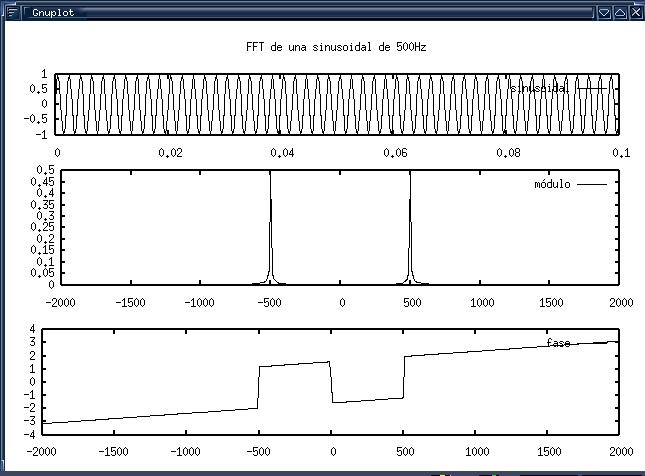
\includegraphics[width=0.8\textwidth]{imagenes/fftview1.m.eps}}
\subfigure[Ejemplo de FFT aplicado a una funci�n escal�n]{%
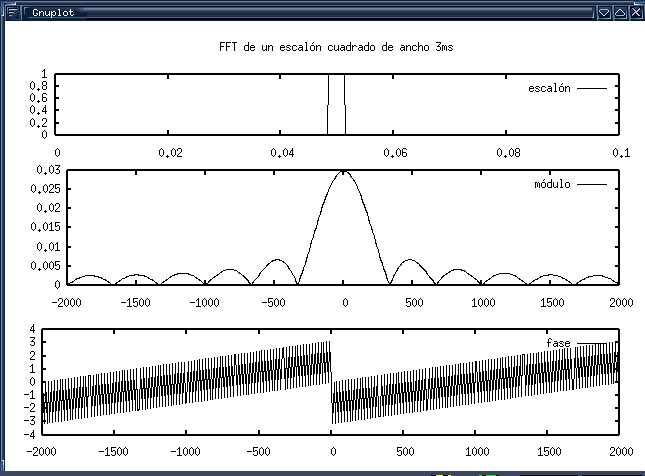
\includegraphics[width=0.8\textwidth]{imagenes/fftview2.m.eps}}
\end{figure}

% estar�a bien poner un filtro de ejemplo, antes y despu�s de pasar
% una se�al por el.

\section{Tratamiento de im�genes}

\index{Octave!tratamiento de im�genes}

Por  �ltimo veamos  un  ejemplo  de c�mo  se  pueden cargar,  realizar
modificaciones,  visualizar y  salvar im�genes  usando las  rutinas de
octave.  Con  esto  podremos  realizar muchas  operaciones  �tiles  en
procesado, realzado y an�lisis de  im�genes, �tiles en muchas �reas de
las ciencias.

En primer lugar suponemos sabido que una imagen se puede entender como
una matriz  donde cada punto tiene  un color diferente. Cada  punto se
llama {\em p�xel}. Hay muchas  formas de representar pixeles, y octave
maneja tres de ellas, que son las siguientes:

\begin{description}

\item[escala de grises]  En una imagen en escala de  grises cada p�xel
se  representa  por  un  valor de  punto  flotante  comprendido  entre
0,  que  significa  negro,  y  1, que  significa  blanco.  Por  tanto,
la  representaci�n  de una  imagen  es  una  matriz llena  de  valores
comprendidos entre 0 y 1. En  este caso, un valor de 0.5 representar�a
un color gris que tiene partes  iguales de blanco y negro mientras que
un valor de  0.2 representar�a un color  que tiene 20\% de  negro y el
resto de blanco.

\item[color RGB] Cualquier  color en la naturaleza  se puede aproximar
(no es una  correspondencia exacta) como suma de  sus tres componentes
de color, a saber:  rojo (R, red), verde (G, green)  y azul (B, blue).
De esta forma, cada p�xel de  una imagen en color se puede representar
como  un terna  de valores  de sus  tres componentes.  Por tanto,  una
imagen en formato  RGB son tres matrices del mismo  tama�o, donde cada
una almacena los valores de una componente.

\item[color  indexado]   Como  en  una  imagen   suele  haber  colores
repetidos,  esta representaci�n  lista  por un  lado  los colores,  de
manera consecutiva y  sin repetirse, y por otro lado  los pixels, cuyo
color  se  almacena  buscando  el  valor en  la  tabla  de  colores  y
almacenando el �ndice correspondiente en el vector.

\end{description}

La  funci�n  usada  para  representar im�genes  en  pantalla  es  {\tt
imshow()}. En  primer lugar  la usaremos  para representar  valores en
escala de grises. Vamos a probar creando una matriz que tenga variedad
de valores y present�ndola. Veamos el ejemplo de uso de esta funci�n:

\begin{verbatim}
octave:15> a=0:0.01:1;
octave:16> ma=a'*a;
octave:17> imshow(ma,2)
octave:18> imshow(ma,16)
octave:19> imshow(ma,256)
\end{verbatim}

\begin{figure}[htbp]
\centering
\subfigure[2 niveles]{%

\includegraphics[width=0.32\textwidth]{imagenes/image1a.m.eps}}
\subfigure[16 niveles]{%

\includegraphics[width=0.32\textwidth]{imagenes/image1b.m.eps}}
\subfigure[256 niveles]{%

\includegraphics[width=0.32\textwidth]{imagenes/image1c.m.eps}}
\caption[Gradiente visualizado a varios niveles de gris]%
{El gradiente anterior visualizado a varios niveles de gris}
\end{figure}

Observando la matriz  {\tt ma} observamos que todos  sus valores est�n
en el  rango $[0,1]$. Si  vemos su tama�o,  vemos que es  100x100. Las
diferentes  llamadas  a {\tt  imshow}  se  diferencian en  el  segundo
par�metro  que representa  el n�mero  de colores  discretos en  el que
presentar� la imagen continua. En el primer caso veremos solamente dos
colores, en la segunda 16 y en la tercera 256.

Probemos ahora  a trabajar con  una imagen  en color. La  funci�n {\tt
loadimage()}  se  utiliza para  cargar  im�genes  de un  archivo.  Las
im�genes se devuelven en formato  indexado, donde {\tt c} representar�
la matriz y {\tt cmap} representar� los colores. Veamos el ejemplo:

\begin{verbatim}
octave:26> [c,cmap]=loadimage("tux.img");
octave:27> imshow(c,cmap)
\end{verbatim}

Como  ver�s, se  visualiza con  la misma  funci�n. Ahora,  usemos esta
imagen como  base para  jugar un poco.  Primero, transform�mosla  a un
formato  m�s  manejable. Empezaremos  pas�ndola  a  {\tt RGB}  con  la
funci�n {\tt ind2rgb}  transforma la imagen de indexada  a RGB. Luego,
con {\tt imshow} la representaremos.

\begin{verbatim}
ctave:28> [r,g,b]=ind2rgb (c,cmap);
octave:29> imshow(r,g,b)
octave:30> imshow(g,r,b)
octave:31> imshow(b,g,r)
\end{verbatim}

\begin{figure}[htbp]
\centering
\subfigure[{\tt imshow(r,g,b)}]{%

\includegraphics[width=0.32\textwidth]{imagenes/image2a.m.eps}}
\subfigure[{\tt imshow(g,r,b)}]{%

\includegraphics[width=0.32\textwidth]{imagenes/image2b.m.eps}}
\subfigure[{\tt imshow(b,g,r)}]{%

\includegraphics[width=0.32\textwidth]{imagenes/image2c.m.eps}}
\caption[Imagen en color cambiando las componentes RGB]%
{Los colores de la imagen vienen representados por sus componentes
RGB. Si se invierten, los colores cambian.}
\end{figure}

Observamos  que  cada  canal  contiene sus  valores,  y  cambiando  el
orden hacemos  creer a  imshow que  los valores  son diferentes  y nos
muestra im�genes  con los colores trasladados.  Podemos probar tambi�n
sustituyendo las matrices {\tt r}, {\tt g}  o {\tt b} por unos o ceros
y  comprobar el  efecto de  quitar o  a�adir canales.  El trabajo  con
im�genes RGB  es complejo, as�  que usaremos  una imagen en  escala de
grises para seguir efectuando nuestras pruebas.

\begin{verbatim}
octave:32> g=ind2gray (c,cmap);
octave:35> imshow(g,2)
octave:36> imshow(g,4)
octave:37> imshow(g,16)
octave:65> imshow(g,256)
\end{verbatim}

\index{Octave!filtrado de im�genes}

Comenzaremos los an�lisis con  un filtrado/realzado. Estas operaciones
se realizan  barriendo todos  los p�xels  de la  imagen y  creando una
nueva imagen  donde cada p�xel  es una  ponderaci�n de los  valores de
cada  p�xel y  sus vecinos  seg�n unas  matrices preestablecidos.  Las
matrices

\[
\begin{array}{ccc}
\frac{1}{5}\left( \begin{array}{ccc}
0 & 1 & 0\\
1 & 1 & 1\\
0 & 1 & 0
\end{array}\right)  & \left( \begin{array}{ccc}
0 & -1 & 0\\
-1 & 5 & -1\\
0 & -1 & 0
\end{array}\right)  & \left( \begin{array}{ccc}
0 & -1 & 0\\
-1 & 4 & -1\\
0 & -1 & 0
\end{array}\right) \\
\textrm{Filtro pasa-baja} & \textrm{Filtro pasa-alta} & \textrm{Detector de bordes}
\end{array}\]

Ahora veamos como  se aplicar�a un filtro. Este filtro  es el primero,
que  genera una  imagen  donde  cada p�xel  es  un  promedio entre  el
correspondiente en  la imagen original  y sus cuatro vecinos  por cada
lado.

\begin{verbatim}
octave:41> h=zeros(256,256);
octave:42> for i=2:255;
>             for j=2:255;
>                h(i,j)=(g(i,j)+g(i-1,j)+g(i+1,j)+ \
>                       g(i,j-1)+g(i,j+1))/5;
>             endfor;
>          endfor;
octave:43> imshow(g,256)
octave:44> imshow(h,256)
\end{verbatim}

Mostrando la imagen original y  retocada comprobamos que el efecto que
tiene es el de suavizar los bordes de la imagen, el de emborronarla.

Habr�s notado que  has tenido que esperar un rato  (seg�n la velocidad
de  tu  m�quina)   durante  un  buen  rato  para   ver  el  resultado.
Este  procedimiento   es  optimizable  atendiendo  a   las  especiales
caracter�sticas de manejo  de matrices de octave. En vez  de hacer las
operaciones  elemento  a  elemento  con  sus  superiores,  inferiores,
izquierdo  y   derecho,  podemos  hacerlas   globalmente,  simplemente
trabajando con  las matrices  completas y operando  con ellas  con sus
desplazadas una posici�n hacia arriba,  abajo, izquierda y derecha. El
ejemplo esta aqu�  y comprobar�s que el resultado  es notablemente m�s
r�pido.

\begin{verbatim}
octave:44> i=2:255;
octave:45> h=(g(i,i)+g(i-1,i)+g(i+1,i)+g(i,i-1)+g(i,i+1))/5;
octave:46> imshow(g,256)
octave:47> imshow(h,256)
\end{verbatim}

Comprobemos ahora los otros dos filtros. El siguiente filtro pasa-alta
se  implementar�a as�.  El resultado,  al contrario  que el  anterior,
acent�a los bordes en la  imagen, resultando los peque�os detalles m�s
destacados a simple vista.

\begin{verbatim}
octave:44> i=2:255;
octave:45> h=5*g(i,j)-g(i-1,j)-g(i+1,j)-g(i,j-1)-g(i,j+1);
octave:46> imshow(g,256)
octave:47> imshow(h,256)
\end{verbatim}

\begin{figure}[htbp]
\centering
\subfigure[Imagen original]{%

\includegraphics[width=0.32\textwidth]{imagenes/image3a.m.eps}}
\subfigure[Filtro pasa-baja]{%

\includegraphics[width=0.32\textwidth]{imagenes/image3b.m.eps}}
\subfigure[Filtro pasa-alta]{%

\includegraphics[width=0.32\textwidth]{imagenes/image3c.m.eps}}
\caption[Imagen tras aplicarle un filtro pasa-baja y pasa-alta]%
{Cuando aplicamos un filtro pasa-baja se suaviza la imagen y si 
aplicamos un pasa-alta, sus detalles se acent�an.}
\end{figure}

\index{Octave!detecci�n de bordes}

Y por �ltimo, el  detector de bordes, que lo que  hace es presentar de
color blanco  las zonas que en  la imagen original tienen  cambios m�s
r�pidos, mientras que las zonas  m�s homog�neas las presenta en negro.
Con esto, conseguimos detectar bordes acusados en la imagen.

\begin{verbatim}
octave:44> i=2:255;
octave:45> h=5*g(i,j)-g(i-1,j)-g(i+1,j)-g(i,j-1)-g(i,j+1);
octave:46> imshow(g,256)
octave:47> imshow(h,256)
\end{verbatim}

\begin{figura}{image4.m}{.8}
\caption{Imagen tras aplicar detector de bordes.}
\end{figura}

%Autor: amd77

\chapter{GNUplot}


Gnuplot es el programa encargado de hacer  las gr�ficas 2D y 3D que se
visualizaban  en  Octave.  Gnuplot  es un  programa  independiente  de
Octave, que  usado por s�  mismo te permite hacer  representaciones de
funciones  continuas  y  de  tablas  de  datos.  Octave  s�lo  usa  un
subconjunto de las funcionalidades de Gnuplot.

La primera caracter�stica  de Gnuplot es que es muy  similar a Octave
en funcionamiento,  es decir, que  posee una interfaz de  comandos muy
poderosa que  tambi�n puedes utilizar escribiendo  scripts. Esta forma
de trabajar tiene  sus desventajas y sus ventajas.  Las desventajas es
que necesitas  una curva  de aprendizaje m�s  lenta, donde  tienes que
haberte mirado  por lo  menos la  descripci�n de  uno de  los comandos
({\tt plot}) para  poder empezar a hacer algo.  Cuando est�s tanteando
datos mejor que uses otro programa  que te permita hacer las cosas m�s
interactivamente. Pero cuando ya tienes claro lo que tienes que hacer,
por ejemplo, sobre una tabla de datos,  y tienes 100 tablas de datos a
las que hacer  lo mismo, poder hacer  un script puede ser  de una gran
ayuda.

La  otra  caracter�stica  destacable  de Gnuplot  es  la  variedad  de
formatos de  salida de que  dispone, que  se pueden seleccionar  en el
script.  Te permite  exportar  a formatos  vectoriales (xfig,  {\TeX},
postscript),  formatos  bitmap (png,  pbm),  o  formatos de  impresora
(epson, hp, etc).  Con esto puedes tener tu gr�fica  retocada por xfig
en tu publicaci�n en  LaTeX, o bien puesta en tu p�gina  web (png) y o
bien impresa directamente en una impresora.

Al ejecutar gnuplot en un shell entramos a su l�nea de comandos:

\begin{verbatim}
alberto@mencey:~$ gnuplot

	G N U P L O T
	Linux version 3.7
	patchlevel 1
	last modified Fri Oct 22 18:00:00 BST 1999

	Copyright(C) 1986 - 1993, 1998, 1999
	Thomas Williams, Colin Kelley and many others

	Type `help` to access the on-line reference manual
	The gnuplot FAQ is available from
	<http://www.ucc.ie/gnuplot/gnuplot-faq.html>

	Send comments and requests for help to <info-gnuplot@dartmouth.edu>
	Send bugs, suggestions and mods to <submit@bugs.debian.org>


Terminal type set to 'x11'
gnuplot> 
\end{verbatim}

Como fuente  de ayuda teclea  {\tt help}  desde dentro del  programa y
despu�s de una pantalla introductoria te saldr� un prompt sobre el que
podr�s escribir, o bien un nombre que elegir�s de los topics que se te
presentan, o bien un nombre de comando si quieres conocer su sintaxis.

Como has  visto, el formato  de salida es  x11 (visualizar en  las X).
Para ver un listado de los  diferentes tipos de salida disponibles usa
{\tt set terminal}.

\section{Representaci�n de expresiones anal�ticas}

La  parte  m�s sencilla  y  pr�ctica  de  Gnuplot es  la  presentaci�n
de  funciones  continuas, tanto  en  forma  expl�cita {\tt  y=f(x)}  o
{\tt  z=f(x,y)},  como  puede  ser en  forma  param�trica:  curvas  2D
{\tt (x,y)=f(t)},  curvas 3D  {\tt (x,y,z)=f(u)}, superficies  3D {\tt
(x,y,z)=f(u,v)}.

Con  {\tt help  functions} tenemos  un  listado de  las funciones  que
admite. Una  gran desventaja que  tiene es que muestrea  las funciones
a  intervalos  regulares,  por  tanto,  no  hace  ning�n  an�lisis  de
discontinuidades  (lo que  se nota  en, por  ejemplo, la  funci�n {\tt
floor}), aunque s� se puede  configurar para que reduzca el intervalo.
Si queremos  imponer cual ser� el  rango del eje  X o el Y  lo ponemos
entre corchetes antes de la funci�n. Algunos ejemplos:


\begin{verbatim}
gnuplot> plot x                        # identidad
gnuplot> plot abs(x)                   # valor absoluto
gnuplot> plot x**2                     # par�bola
gnuplot> plot [-1:1] sqrt(1-x**2)      # semicircunferencia
gnuplot> plot [] [-0.1:1.1] exp(-x**2) # gaussiana
gnuplot> plot [-1:4] gamma(x)          # funci�n gamma
gnuplot> plot floor(x)                 # funci�n redondeo hacia abajo
gnuplot> plot x-floor(x)               # diente de sierra
gnuplot> splot x**2+y**2               # plot en 3D
gnuplot> splot sqrt(1-x**2+y**2)              
gnuplot> set isosamples 20,20          # cambia la resoluci�n
gnuplot> replot                 
gnuplot> set isosamples 50,50          # cambia la resoluci�n
gnuplot> set contour		       # activa l�neas de nivel
gnuplot> replot
gnuplot> set parametric                # modo param�trico 

	dummy variable is t for curves, u/v for surfaces
gnuplot> set samples 500                   # mejor resoluci�n (+lento)
gnuplot> plot sin(7*t),cos(5*t)            # lissajous en 2D
gnuplot> splot sin(5*u),sin(6*u),sin(7*u)  # lissajous en 3D
gnuplot> set samples 100                   # menor resoluci�n (+r�pido)
gnuplot> splot cos(u)*cos(v),cos(u)*sin(v),sin(u)  # esfera en 3D
\end{verbatim}

\section{Representaci�n de archivos de datos}

 Gnuplot  tambi�n tiene un  modo para trabajar con  archivos de
datos con m�ltiples columnas. Cuando los  archivos de datos tienen 1 �
2  columnas  se  presentan  directamente.  Si  un  archivo  tiene  m�s
de  2 columnas  se  pueden presentar  columnas arbitrariamente,  hacer
operaciones matem�ticas  sencillas entre  columnas. Veamos esto  en un
ejemplo real (bastante prolijo) donde  un servidor genera una l�nea de
log de  load, logins y  carga de cpu, a  cada hora y  queremos obtener
gr�ficas que muestren la evoluci�n en el tiempo 

\begin{verbatim}
# Ejemplo para la monitorizaci�n de carga de un servidor en el tiempo

set title "Convex     November 1-7 1989    Circadian"
set key left box
set xrange[-1:24]
plot 'gnuplot.dat' using 2:4 title "Logged in" with impulses,\
     'gnuplot.dat' using 2:4 title "Logged in" with points
pause -1 "Hit return to continue"

set xrange [1:8]
#set xdtic
set title "Convex     November 1-7 1989"
set key below
set label "(Weekend)" at 5,25 center
plot 'gnuplot.dat' using 3:4 title "Logged in" with impulses,\
     'gnuplot.dat' using 3:5 t "Load average" with points,\
     'gnuplot.dat' using 3:6 t "%CPU used" with lines
set nolabel
pause -1 "Hit return to continue"
reset
\end{verbatim}

 Como �ltimo  ejemplo, vamos a probar un script  donde se hacen
ajustes por el m�todo de m�nimos  cuadrados con Gnuplot. En el ejemplo
se realizan ajustes a una recta  variando los pesos, pero el m�todo de
ajuste que utiliza Gnuplot permite  poner cualquier funci�n de ajuste,
simplemente definiendo las variables y constantes y dando unos valores
iniciales a las constantes. 

\begin{verbatim}
# ajustes por m�nimos cuadrados en Gnuplot 

y(x) = a*x + b   # funci�n a la que se ajustar�
a = 0.0          # valores iniciales
b = 0.0          # de los par�metros

fit y(x) 'gnuplot-fit.dat' via a, b
set title 'Ajuste sin pesar'
plot 'gnuplot-fit.dat', y(x)
pause -1 "Pulsa enter para continuar"

fit y(x) 'gnuplot-fit.dat' using 1:2:3 via a, b
set title 'Ajuste con mayor peso en bajas temperaturas'
plot 'gnuplot-fit.dat', y(x)
pause -1 "Pulsa enter para continuar"

fit y(x) 'gnuplot-fit.dat' using 1:2:4 via a, b
set title 'Ajuste con mayor peso a altas temperaturas'
plot 'gnuplot-fit.dat', y(x)
pause -1 "Pulsa enter para continuar"

fit y(x) 'gnuplot-fit.dat' using 1:2:5 via a, b
set title 'Ajuste con peso correspondiente a error experimental'
plot 'gnuplot-fit.dat' using 1:2:5 with errorbars, y(x)
pause -1 "Pulsa enter para continuar"
\end{verbatim}



%Autor: miguev

\chapter{GNU R}
\label{r.tex}

\index{R}
\index{GNU R}

\section{Introducci�n}

%%%%%% Traducido de la web de R en http://www.r-project.org

{\sf R}  es a  la vez un  entorno y un  lenguaje de  programaci�n para
realizar c�lculos y gr�ficos estad�sticos. Es un proyecto GNU similiar
al  sistema {\sf  S}  desarrollado en  Bell Laboratories  (formalmente
AT\&T, ahora  Lucent Technologies)  por John  Chambers y  sus colegas.
{\sf R} puede  considerarse como una implementaci�n  diferente de {\sf
S}. Hay diferencias importantes entre ambos, pero mucho c�digo escrito
para el sistema {\sf S} puede ejecutarse en {\sf R} sin modificarlo.

{\sf  R}  proporciona  una  amplia  variedad de  t�cnicas  gr�ficas  y
estad�sticas (regresiones  lineales y no lineales,  tests estad�sticos
cl�sicos, an�lisis  de series temporales,  clasifiaciones, clustering,
etc.)  y adem�s  es  muy extensible.  El lenguaje  {\sf  S} suele  ser
utilizado para la investigaci�n en  metodolog�a estad�stica, y {\sf R}
proporciona una alternativa de c�digo abierto para esta actividad.

Uno de  los puntos fuertes de  {\sf R} es  la facilidad con la  que se
pueden  producir  gr�ficas  de  buen dise�o  y  calidad  de  imprenta,
incluyendo  s�mbolos y  f�rmulas  matem�ticas  donde sean  necesarias.
Aunque {\sf R}  pone un gran cuidado en las  opciones por defecto para
el dise�o de las gr�ficas, el  usuario puede tener control total sobre
�stas.

{\sf R}  es Software  Libre, disponible  bajo los  t�rminos de  la GNU
General Public  License de  la Free Software  Foundation, en  forma de
c�digo fuente. Se puede compilar y  ejecutar en una amplia variedad de
plataformas  UNIX  (incluyendo  Linux  y  FreeBSD),  MacOS  y  Windows
9x/NT/2000.

El  c�digo  fuente  de  {\sf  R} se  puede  descargar  del  sitio  web
del  proyecto {\sf  R} ({\tt  http://www.r-project.org}), as�  como su
documentaci�n. Adem�s de la  documentaci�n oficial (en ingl�s) existen
otros  documentos {\em  contribuidos} entre  los que  se encuentra  la
traducci�n  al  espa�ol  de  ``An Introduction  to  R''  y  ``Gr�ficos
Estad�sticos con R''. \index{R!documentaci�n}  Estos y m�s manuales se
encuentran en el CRAN (Comprehensive R Archive Network), concretamente
en {\tt http://cran.r-project.org/other-docs.html}

%%%%%%

\section{El entorno R}

\index{R!entorno}

{\sf  R} es  un conjunto  integrado de  utilidades para  manipulaci�n,
c�lculo  y  representaci�n  de  datos.  Decimos  que  {\sf  R}  es  un
{\em entorno}  porque es  un sistema  dise�ado para  ser completamente
coherente.  El  entorno  de   {\sf  R}  proporciona  facilidades  para
manipulaci�n  y almacenamiento  de  datos,  operaciones con  variables
indexadas  (como vectores  y matrices),  an�lisis y  representaci�n de
datos, un lenguaje de programaci�n  bien desarrollado (con todo lo que
cabe esperar  de un lenguaje  de programaci�n) y una  amplia colecci�n
integrada y coherente de utilidades para an�lisis de datos.

Aunque mucha  gente utiliza {\sf  R} como un sistema  estad�stico, sus
autores  prefieren considerarlo  como ``un  entorno en  el que  se han
implementado muchas  t�cnicas estad�sticas, cl�sicas y  modernas''. La
mayor�a  de la  estad�stica cl�sica  y muchas  de los  �ltimos m�todos
est�n disponibles en  {\sf R}, aunque posiblemente  tendr�s que buscar
un rato para encontrarlas.

La forma de trabajar  con {\sf R} es distinta a  la de otros programas
como {\tt SPSS}. En {\sf R}, un an�lisis estad�stico se realiza en una
serie de pasos, con unos resultados intermedios que se van almacenando
en  objetos,   para  ser   observados  o   analizados  posteriormente,
produciendo unas salidas  m�nimas. En {\tt SPSS} se  obtendr�a de modo
inmediato  una  salida copiosa  para  cualquier  an�lisis. Esto  puede
parecer a primera  vista una terrible incomodidad,  pero si tuvi�ramos
que  trabajar en  una m�quina  poco potente  r�pidamente nos  dar�amos
cuenta de que puede resultar muy ventajosa la sencillez del entorno de
{\sf  R} (un  entorno de  comandos) y  la posibilidad  de ver  en cada
momento exactamente lo  que se necesita, sin  excesos que desperdicien
recursos del sistema.

A�n as�, la mejor  manera de trabajar con R es  en un entorno gr�fico,
con un sistema de ventanas como  X-Window, de forma que puedas ver las
gr�ficas en el momento de generarlas.

Veamos c�mo se trabaja con {\sf  R} us�ndolo. En primer lugar conviene
crear un  directorio y entrar en  �l antes de comenzar  una sesi�n con
{\sf  R}, que  en  �ste almacena  siempre en  el  directorio donde  se
ejecutan unos ficheros donde almacena  los objetos, datos, funciones y
comandos ejecutados.  Esto puede sernos  muy �til en  trabajos largos,
podemos  interrumpir la  sesi�n con  {\sf  R} en  cualquier momento  y
recuperarla luego donde mismo la dejamos.

Hemos considerado a lo largo de  este curso que el s�mbolo del sistema
Linux/UNIX es  {\tt \$}. Vamos a  considerar ahora que el  s�mbolo del
prompt  {\sf R}  es {\tt  $>$}. \index{R!prompt}  Abre un  emulador de
terminal dentro del entorno gr�fico y ejecuta los siguientes comandos:

\begin{verbatim}
$ mkdir sesion_R
$ cd sesion_R
$ R

R : Copyright 2002, The R Development Core Team
Version 1.5.1  (2002-06-17)

R is free software and comes with ABSOLUTELY NO WARRANTY.
You are welcome to redistribute it under certain conditions.
Type `license()' or `licence()' for distribution details.

R is a collaborative project with many contributors.
Type `contributors()' for more information.

Type `demo()' for some demos, `help()' for on-line help, or
`help.start()' for a HTML browser interface to help.
Type `q()' to quit R.

> 
\end{verbatim}

El prompt de {\sf R} indica  el entorno que est� esperando tus �rdenes
para ejecutarlas. Para salir del entorno de {\sf R} puedes utilizar la
funci�n {\tt q()}  o pulsar {\tt C-d}, entonces {\sf  R} te preguntar�
si  deseas  guardar el  {\em  espacio  de  trabajo},  que es  toda  la
informaci�n sobre la sesi�n que quieres cerrar:

\index{R!sesiones}

\begin{verbatim}
> q()
Save workspace image? [y/n/c]: 
\end{verbatim}

Para salir guardando la sesi�n pulsa {\tt y}, para salir sin guardarla
pulsa {\tt n} y para para cancelar la salida pulsa {\tt c}. Si guardas
la  sesi�n al  salir quedar�  almacenada en  el directorio  en el  que
ejecutaste {\tt R},  y ser� autom�ticamente recuperada  la pr�xima vez
que ejecutes {\tt R} dentro del directorio en cuesti�n.

{\sf R} dispone de un sistema de ayuda similar a las p�ginas de manual
de  Linux/UNIX. Cuando  necesites informaci�n  sobre una  funci�n, por
ejemplo {\tt  solve}, ejecuta la  funci�n {\tt help()}  pas�ndole como
par�metro el nombre de la funci�n que quieras consultar. Tambi�n existe
una forma m�s corta: {\tt ?funci�n}:

\index{R!ayuda}
\index{R!help@{\tt help()}}

\begin{verbatim}
> help (solve)
> ?solve 
\end{verbatim}

Normalmente  puedes  ver  la  documentaci�n tambi�n  en  el  navegador
web. Si  ejecutas {\tt  help.start()} deber�a  abrirse una  ventana de
navegador  con la  documentaci�n en  formato HTML  por la  cual puedes
navegar para buscar lo que necesites.

Otra forma muy interesante de buscar  ayuda dentro del entorno de {\sf
R}  es pasarle  una  palabra  a la  funci�n  {\tt help.search()}.  Por
ejemplo, para buscar  una funci�n que resuelva  sistemas de ecuaciones
puedes empezar por buscar la palabra {\tt solve}.

\index{R!b�squeda}
\index{R!help.search@{\tt help.search()}}

\begin{verbatim}
> help.search ("solve")

Help files with alias or title matching `solve',
type `help(FOO, package = PKG)' to inspect entry `FOO(PKG) TITLE':

backsolve(base)         Solve an Upper or Lower Triangular System
qr(base)                The QR Decomposition of a Matrix
solve(base)             Solve a System of Equations
\end{verbatim}

De un  primer golpe  ya sabes  que el  paquete {\tt  base} de  {\sf R}
tiene  funciones para  resolver  sistemas  triangulares (superiores  o
inferiores), descomponer matrices  en la forma QR  y resolver sistemas
de ecuaciones (cualesquiera).

{\sf  R} proporciona  algunas  demostraciones  sobre sus  capacidades.
Para  ir abriendo  el apetito  ejecuta la  funciones que  muestran las
demostraciones con gr�ficos e im�genes:

\begin{verbatim}
> demo (graphics)
> demo (images)
\end{verbatim}

%\begin{figure}[hbtp]
%\centering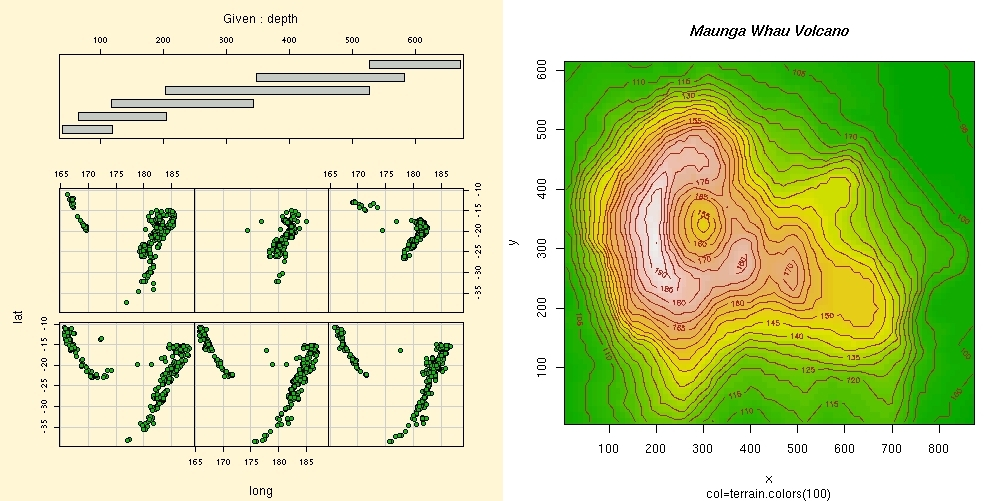
\includegraphics[width=\textwidth]{imagenes/r_demos.eps}
%\index{R!demos}
%Demostraciones sobre gr�ficos e im�genes
%\end{figure}

\begin{figura}{r_demos}{1}
\index{R!demos}
Demostraciones sobre gr�ficos e im�genes
\end{figura}


\section{El lenguaje {\sf R}}

\index{R!lenguaje}

{\sf R} es tambi�n lenguaje de  programaci�n en toda regla, con el que
puedes escribir  programas que  procesen ficheros  de datos  y generen
an�lisis y representaciones de los datos.

Al igual que  la mayor�a de lenguajes basados en  UNIX, el lenguaje de
{\sf R} distingue entre may�sculas y min�sculas. Esto es, {\tt esto} y
{\tt  Esto} son  s�mbolos  distintos y  pueden  referirse a  variables
distintas. En {\sf  R} los nombres de variables pueden  tener letras y
n�meros  (como en  casi cualquier  lenguaje), aunque  {\bf no}  pueden
tener el  subrayado ({\tt \_}),  pero en su  lugar s� pueden  tener el
punto.  De hecho  se suele  utilizar  el punto  para separar  palabras
en  los  nombres  de  las  variables en  {\sf  R},  por  ejemplo  {\tt
hoja.de.datos}.

\index{R!�rdenes}
\index{R!comandos}

Las �rdenes  (o comandos) elementales son  expresiones o asignaciones.
Si ejecutas  una expresi�n como comando  �sta se eval�a y  se imprime,
pero su valor se pierde. En una asignaci�n la expresi�n se eval�a y su
valor se almacena en la varbiable, pero no se imprime.

Los comandos se  separan con el caracter  de punto y coma  ({\tt ;}) o
simplemente  con una  salto  de  l�nea. Puedes  agrupar  una serie  de
comandos  encerr�ndolos entre  llaves,  de esta  forma puedes  definir
funciones como veremos m�s adelante. Tambi�n puedes poner comantarios,
\index{R!comentarios} casi  donde quieras\footnote{No puedes  meter un
comentario dentro  de una cadena  de caracteres (formar�a parte  de la
cadena), ni en medio de la lista de argumentos en la definici�n de una
funci�n}, poniendo  una almohadilla ({\tt \#})  y todo lo que  la siga
hasta el final de l�nea ser� obviado por el int�rprete de {\sf R}.

Si dejas  un comando a medias  {\sf R} se  dar� cuenta, y en  lugar de
mostrarte el prompt  $>$ te mostar� {\tt +} para  avisarte de que est�
esperando por el final del comando.

Otra caracter�stica  interesante de {\sf  R} (al menos  en plataformas
Linux/UNIX)  es  la  posibilidad  de  editar  la  l�nea  de  comandos.
Esto  incluye  el  t�pico  historial   de  comandos,  que  te  permite
repetir  los comandos  sin tener  que  volver a  teclearlos. Tan  solo
utiliza los  cursores arriba y  abajo para recuperar los  comandos que
hayas tecleado.  \index{R!historial} Adem�s este historial  de comando
queda  almacenado en  la  sesi�n  cuando sales  del  entorno {\sf  R},
concretamente en  un fichero  {\tt .Rhistory}  en el  directorio donde
ejecutaste en entorno {\sf R}.

Pero si necesitas usar una serie un poco larga de comandos seguramente
te canses de tener  que darle a los cursores. Para  estos casos lo que
necesitas  es un  script en  el que  escribes los  comandos a  modo de
programa. Luego para ejecutar los  comandos escritos en �l utilizas la
funci�n {\tt  source ()} del  entorno pas�ndole el nombre  del fichero
donde escribiste los comandos:

\index{R!leer comandos de un fichero}
\index{R!source@{\tt source()}}

\begin{verbatim}

> source ("script.R")

\end{verbatim}

Del  mismo modo  que puedes  tomar la  entrada de  un fichero  tambi�n
puedes redireccionar la salida hacia otro fichero, con la funci�n {\tt
sink()}. Para almacenar la salida en el fichero {\tt salida.txt} 
ejecuta el comando:

\index{R!volcar en un fichero}
\index{R!sink@{\tt sink()}}

\begin{verbatim}

> sink ("salida.txt")

\end{verbatim}

Para devolver  la salida al  int�rprete utiliza la misma  funci�n {\tt
sink  ()}  pero sin  pasarle  ning�n  par�metro.  En el  fichero  {\tt
iodemo.R}  tienes un  ejemplo de  esto. 

\begin{ejemplo}{iodemo.R}{Uso de {\tt sink()}}
Este script lee  una tabla que est� almacenada en  un fichero de texto
llano ({\tt muestra.dat}, que usaremos para los ejemplos) y extrae dos
variables  de ella.  Para  ambas variables  muestra  un breve  resumen
estad�stico, pero guarda uno en el  fichero {\tt salida.txt} y el otro
lo muestra en el entorno {\sf R}.
\end{ejemplo}

Entra en el directorio donde tengas el fichero y ejecuta en el entorno
{\sf R}

\begin{verbatim}
> source ("iodemo.R")
\end{verbatim}

\section{Vectores}

\index{R!vectores}

{\sf R} realiza las operaciones sobre las llamadas {\em estructuras de
datos}, de las cuales la m�s  simple es el vector num�rico. Para crear
un vector con  los 5 primeros n�meros enteros  positivos utilizamos la
funci�n {\tt  c()} que  combina los objetos  recibidos para  formas un
vector:

\begin{verbatim}
> x <- c (1, 2, 3, 4, 5)
> x
[1] 1 2 3 4 5
\end{verbatim}

\index{R!asignaci�n, operador de}

En efecto, el operador de asignaci�n no se parece para nada a un signo
de igualdad. De  hecho es una flecha, que est�  indicando que el valor
de lo que hay a su derecha debe asignarse a lo que hay a su izquierda.
Si le das la vuelta a la flecha funciona al rev�s:

\begin{verbatim}
> c (6, 7, 8, 9, 10) -> y
> y
[1]  6  7  8  9 10
\end{verbatim}

Cuando  ejecutas  el  nombre  de  un  objeto  como  comando,  {\sf  R}
interpreta que deseas  ver su contenido y entonces  ejecuta la funci�n
{\tt print()} sobre  el objeto en cuesti�n. Esto  funciona s�lo cuando
est�s  dentro del  entorno {\sf  R} y  tecleas el  nombre del  objeto.
\index{R!print@{\tt print()}}
Cuando quieras imprimir  el objeto desde un fichero  de comandos (como
hacemos en {\tt iodemo.R}) has de utilizar la funci�n {\tt print()}.

Dado que la funci�n {\tt c()} combina objetos para formar vectores, 
tambi�n puede combinar varios vectores para formar un nuevo vector
que es el resultado de concatenar los anteriores:

\begin{verbatim}
> z <- c (x, y)
> z
 [1]  1  2  3  4  5  6  7  8  9 10
\end{verbatim}

Las  operaciones  usuales  entre  vectores  se  definen  ``elemento  a
elemento'':

\index{R!vectores!operaciones elementales}

\begin{verbatim}
> x + 2
[1] 3 4 5 6 7
> 2 * x
[1]  2  4  6  8 10
> x + y
[1]  7  9 11 13 15
> x - y
[1] -5 -5 -5 -5 -5
> x * y
[1]  6 14 24 36 50
> x / y
[1] 0.1666667 0.2857143 0.3750000 0.4444444 0.5000000
> y / x
[1] 6.000000 3.500000 2.666667 2.250000 2.000000
> x ^ y
[1]       1     128    6561  262144 9765625
> y ^ x
[1]      6     49    512   6561 100000
\end{verbatim}

Pero  entonces �c�mo  se multiplican  escalarmente dos  vectores? Para
esto hay una funci�n llamada  {\tt crossprod}, que permite multiplicar
dos  vectores  (o  matrices).  El operador  \verb|%*%|  es  una  forma
abreviada  de  este  producto.  Formalmente  {\tt  crossprod(x,y)}  es
equivalente a  {\tt t(x) \%*\%  y}, pero  m�s r�pido. La  funci�n {\tt
t()} es la trasposici�n de matrices:

\index{R!vectores!producto escalar}

\begin{verbatim}
> x
[1] 1 2 3 4
> y
[1] 4 5 6 7
> crossprod(x,y)
     [,1]
[1,]   60
> x %*% y
     [,1]
[1,]   60
\end{verbatim}

Adem�s de para guardar datos,  los vectores suelen usarse para definir
series o  secuencias. Para  definir una  secuencia de  n�meros enteros
consecutivos basta  con poner el primer  y el �ltimo separados  por un
caracter de dos puntos:

\index{R!vectores!secuencias}

\begin{verbatim}
> x <- 1:10
> x   
 [1]  1  2  3  4  5  6  7  8  9 10
\end{verbatim}

Pero  para  generar   secuencias  la  mejor  manera   es  utilizar  la
funci�n {\tt  seq()}. Si  le pasas tres  valores num�ricos  le estar�s
especificando el  primer y el  �ltimo elemento  de la secuencia,  y la
diferencia que debe haber entre cada dos elementos consecutivos:

\begin{verbatim}
> y <- seq (-1, 1, .2)
> y
 [1] -1.0 -0.8 -0.6 -0.4 -0.2  0.0  0.2  0.4  0.6  0.8  1.0
\end{verbatim}

Para replicar  un objeto  varias veces, por  ejemplo para  generar una
secuencia  peri�dica,  utiliza la  funci�n  {\tt  rep()} pas�ndole  el
objeto y el n�mero de veces que quieres replicarlo:

\begin{verbatim}
> z <- rep (seq (-1, 1, 1), 5)
> z
 [1] -1  0  1 -1  0  1 -1  0  1 -1  0  1 -1  0  1
\end{verbatim}

Adem�s de vectores num�ricos, {\sf R} permite operar con vectores {\em
l�gicos}.  Los valores  v�lidos  para los  elementos  de los  vectores
\index{R!vectores!vectores l�gicos}
l�gicos son los de la {\em l�gica  triestada}: 
\index{l�gica triestada}
{\tt TRUE}, {\tt FALSE} y {\tt NA} (``Not Available'', no disponible).
Los operadores  l�gicos para manejar  estos valores son {\tt  \&} para
``and'', {\tt |} para ``or'' y {\tt !} para ``not''.

Una forma  de generar  un vector  de valores  l�gicos es  efectuar una
comparaci�n entre un vector num�rico y un valor num�rico:

\begin{verbatim}
> z <- rep (seq (-1, 1, 1), 3)
> z
[1] -1  0  1 -1  0  1 -1  0  1
> z > 0
[1] FALSE FALSE  TRUE FALSE FALSE  TRUE FALSE FALSE  TRUE
\end{verbatim}

Al contrario que  en la mayor�a de lenguajes de  programaci�n, en {\sf
R}  los vectores  se indexan  comenzando por  $1$. Para  acceder a  un
elemento  de un  vector utiliza  la notaci�n  usual de  los corchetes.
Tambi�n puedes acceder a un  subconjunto del vector especificando como
�ndice un vector con las posiciones de los elemenos:

\index{R!vectores!�ndices}
\index{R!vectores!sub�ndices}
\index{R!vectores!indixado}

\begin{verbatim}
> x <- 1:10
> x
 [1]  1  2  3  4  5  6  7  8  9 10
> x[2:5]
[1] 2 3 4 5
> x[8:2]
[1] 8 7 6 5 4 3 2
\end{verbatim}

Tambi�n puedes  acceder a  un subconjunto de  un vector  utilizando un
vector l�gico:

\begin{verbatim}
> x[x > 4]
[1]  5  6  7  8  9 10
\end{verbatim}

Incluso puedes indexar  un vector no palabras, poniendo  nombres a las
posiciones dentro del vector mediante  la funci�n {\tt names()}. Luego
puedes acceder a los elementos mediante los nombres de las posiciones:

\index{R!vectores!nombres}
\index{R!vectores!names@{\tt names()}}

\begin{verbatim}
fruta = c (5, 10, 1, 20)
> fruta <- c (5, 10, 1, 20)
> names (fruta) <- c ("naranja", "pl�tano", "manzana", "�ame")
> fruta[c ("manzana", "naranja")]
manzana naranja 
      1       5 
> fruta
naranja pl�tano manzana    �ame 
      5      10       1      20 
\end{verbatim}

\section{Arrays y matrices}

\index{R!arrays}
\index{R!matrices}

Un   {\em   array}\footnote{a   veces   traducido   por   ``arreglo''}
\index{arreglo} es  una variable indexada multidimensional.  Un vector
es un  array unidimensional  y una matriz  es un  array bidimensional.
{\sf R} proporciona un buen manejo de arrays, sobretodo para matrices.

La dimensi�n de un array es un vector cuya longitud es la dimesi�n del
array,  y  cada uno  de  sus  elementos  es  la ``longitud''  de  cada
dimensi�n en el array. Por  ejemplo, un array con dimesi�n $(3,5,100)$
ser�a como un cubo de $1500$ elementos con $3$ celdas de largo, $5$ de
ancho y $100$ de alto.

\index{R!arrays!dimensi�n}

En la  mayor�a de  lenguajes los  elementos de  un array  se almacenan
``por filas'', lo que significa que el �ndice que avanza m�s r�pido es
el �ltimo. Sin embargo, en {\sf R}  la ordenaci�n se hace al estilo de
FORTRAN, ordenando  los elementos  ``por columnas'', lo  que significa
que el �ndice que avanza m�s r�pido es el primero.

Es importante tener esto en cuenta porque a la hora de crear una 
matriz hay que proporcionar los elementos agrupados por columnas, no 
por filas. Por ejemplo:

\index{R!arrays!por filas}
\index{R!arrays!por columnas}


\begin{verbatim}
> a <- array (c (1:3,-3:-1), dim = c (3,2)) 
> a
     [,1] [,2]
[1,]    1   -3
[2,]    2   -2
[3,]    3   -1
\end{verbatim}

Para  acceder a  los elementos  de una  matriz (o  array) ponemos  los
sub�ndices  entre corchetes  y  separados por  comas.  Si omitimos  el
sub�ndice de las filas (el  primero) obtenemos la columna se�alada por
el segundo sub�ndice, y an�logamente  obtenemos las filas omitiendo el
segundo sun�ndice.

\index{R!arrays!�ndices}
\index{R!arrays!sub�ndices}
\index{R!arrays!indexado}

\begin{verbatim}
> a[1,2]
[1] -3
> a[,2]
[1] -3 -2 -1
> a[1,]
[1]  1 -3
\end{verbatim}

De la misma forma que podemos extraer elementos, filas o columnas de
una matriz tambi�n podemos asignarles valores:

\begin{verbatim}
> a[,2] <- 3:5
> a[,2]
[1] 3 4 5
> a
     [,1] [,2]
[1,]    1    3
[2,]    2    4
[3,]    3    5
\end{verbatim}

Para multiplicar  matrices (o arrays  en general) utiliza  el operador
\verb|%*%| que vimos antes:

\index{R!arrays!producto}
\index{R!matrices!multiplicar}

\begin{verbatim}
> a
     [,1] [,2]
[1,]    1    3
[2,]    2    4
[3,]    3    5
> b = array (1:2, 2:1, dim = c (2,2))
> b
     [,1] [,2]
[1,]    1    1
[2,]    2    2
> a %*% b
     [,1] [,2]
[1,]    7    7
[2,]   10   10
[3,]   13   13
\end{verbatim}

Vimos antes  que si multiplicamos dos  vectores {\tt x} y  {\tt y} (de
igual longitud) utilizando el operador  {\tt \%*\%} el resultado es el
producto  escalar de  los vectores.  En realidad  la operaci�n  {\tt x
\%*\%  y}  es ambigua,  porque  podr�a  significar  $x'  x$ o  $x  x'$
(considerando $x$ un vector columna).  En estos casos de ambig�edad se
considera impl�citamente  que la interpretaci�n deseada  es aquella de
la  que resulte  la  matriz m�s  paque�a,  por lo  que  se obtiene  el
producto escalar $x' x$.

Para  calcular la  matriz $x  x'$ puedes  utilizar las  funciones {\tt
cbind()} y {\tt rbind()}, ya que �stas siempre devuelven matrices. Las
funciones {\tt  cbind} y  {\tt rbind}  toman una  serie de  vectores o
n�meros y los agrupan por columnas o filas en una matriz.

\index{R!matrices!cbind@{\tt cbind()}}
\index{R!matrices!rbind@{\tt rbind()}}

\begin{verbatim}
> x
[1] 1 2 3 4
> y
[1] 4 5 6 7
> x %*% y
     [,1]
[1,]   60
> cbind(x,y)
     x y
[1,] 1 4
[2,] 2 5
[3,] 3 6
[4,] 4 7
> rbind(x,y)
  [,1] [,2] [,3] [,4]
x    1    2    3    4
y    4    5    6    7
> cbind(x) %*% rbind(y)
      
       [,1] [,2] [,3] [,4]
  [1,]    4    5    6    7
  [2,]    8   10   12   14
  [3,]   12   15   18   21
  [4,]   16   20   24   28
\end{verbatim}


\section{Factores: clasificaci�n de datos}

\index{R!factores}
\index{R!clasificaci�n de datos}

Un  {\em factor}  es un  vector  que utilizamos  para especificar  una
clasificaci�n  discreta (agrupamiento)  de  los  componentes de  otros
vectores del mismo tama�o. Para entender  lo que son los factores nada
mejor que un ejemplo claro y sencillo. En el entorno {\sf R} y ejecuta
lo siguiente:

\begin{verbatim}
> edad <- c (13, 16, 15, 17, 17, 18, 16, 16, 15, 16)
> sexo <- c ("hombre", "hombre", "mujer", "hombre", "mujer", "mujer",         
+            "hombre", "mujer", "hombre", "mujer") 
> edad
 [1] 13 16 15 17 17 18 16 16 15 16
> sexo
[1] "hombre" "hombre" "mujer"  "hombre" "mujer"  "mujer"  "hombre" 
[9] "mujer" "hombre" "mujer"
\end{verbatim}

Ahora tienes  una variable {\tt  edad} que  contiene las edades  de 10
personas, y  una variable {\tt  sexo} que define  el sexo de  cada una
de  las  10  personas  anteriores  (en el  mismo  orden)  y  que  toma
�nicamente  los  valores  \verb|"hombre"| y  \verb|"mujer"|.  Vamos  a
calcular  la media  y  la  varianza muestrales  de  la  edad de  estas
personas  clasific�ndolas seg�n  el sexo,  i.e. la  edad media  de los
hombres por un lado y la de las mujeres por otro.

Necesitamos  separar (agrupar)  los  elementos del  vector {\tt  edad}
seg�n los valores que toma el  vector {\tt sexo}. Para esto utilizamos
un factor.  El factor  en realidad  es como  el vector  original, pero
tiene un atributo  a�adido llamado {\tt levels} (niveles)  que son los
distintos  valores que  toman los  elementos del  vector original.  En
el  caso del  vector  {\tt  sexo} los  niveles  son \verb|"hombre"|  y
\verb|"mujer"|. La funci�n  {\tt levels} devuelve la  lista de niveles
que tenga el factor que le pases como par�metro.

\begin{verbatim}
> sexo.factor = factor (sexo)
> sexo.factor
[1] hombre hombre mujer  hombre mujer  mujer  hombre mujer  hombre
Levels:  hombre mujer 
> levels (sexo.factor)
[1] "hombre" "mujer"
\end{verbatim}

Ahora queremos  aplicar unas  funciones, en este  caso {\tt  mean()} y
{\tt  var()}, a  un  vector de  datos  de manera  que  los datos  sean
separados seg�n  un factor.  La funci�n apropiada  para esta  tarea es
{\tt tapply}, y se usa del siguiente modo:

\index{R!tapply@{\tt tapply()}}

\begin{verbatim}
> tapply (edad, sexo.factor, mean)
hombre  mujer 
  15.4   16.4 
> tapply (edad, sexo.factor, var)
hombre  mujer 
   2.3    1.3
\end{verbatim}

As� obtenemos que dentro de esta muestra de 10 personas, la edad media
de los hombres es $15.4$ y  la de las mujeres $16.4$. Volveremos sobre
los factores m�s adelante, as� que aseg�rate de entender al menos este
uso de los mismos. Para mayores detalles consulta la ayuda de {\sf R}.

\section{Listas}

\index{R!listas}

En un  array todos  los elementos  deben ser del  mismo tipo,  i.e. no
puede  ser que  un array  contenga a  la vez  n�meros y  palabras. Sin
embargo la  mayor�a de muestras  contienen datos de  diferentes tipos:
n�meros, palabras, valores l�gicos, intervalos, etc.

Una {\em  lista} en {\sf  R} es una  colecci�n ordenada de  objetos de
cualquier tipo. Es  como un vector, pero con la  diferencia de que sus
elementos pueden ser de distintos tipos. 

Los elementos de una lista est�n  siempre numerados por un sub�ndice y
puedes referirte  a ellos  como con un  vector, pero  usando corquetes
dobles.  As�  si {\tt  L}  es  una lista  {\tt  L[[1]]}  es su  primer
elemento. Pero tambi�n,  al igual que en los  vectores, puedes indexar
los elementos  de una lista d�ndoles  nombres. En caso de  nombrar los
elementos de una lista hay una  forma m�s c�moda de referirse a ellos:
en lugar de {\tt L[["nombre"]]} puedes usar {\tt L\$nombre}.

\index{R!listas!�ndices}
\index{R!listas!nombres}

\begin{verbatim}
> L = list (nombre = "Pepe", esposa = "Pepa", hijos = 3,
+     edades.hijos = c (34,6,12))
> L
$nombre
[1] "Pepe"

$esposa
[1] "Pepa"

$hijos
[1] 3

$edades.hijos
[1] 34  6 12

> L[["nombre"]]
[1] "Pepe"
> L$nombre
[1] "Pepe"
\end{verbatim}

Para concatenar  listas recuerda que  la funci�n {\tt c()}  sirve para
ello.

\section{Hojas de datos}

\index{R!tablas}
\index{R!data frame}
\index{R!frame}
\index{R!hojas de datos}

Una ``hoja  de datos'' (en  ingl�s ``data frame'') es  b�sicamente una
lista de vectores, con algunas restricciones. Los vectores de palabras
son convertidos en factores.

Piensa en una hoja  de datos como su nombre sugiere:  una hoja o tabla
en la que tienes varios datos sobre varios individuos. Las columnas de
la hoja de  datos son los vectores  que la format, y cada  fila es una
lista.

En el  fichero {\tt  muestra.dat} tienes una  hoja de  datos preparada
para ser leida con la funci�n  {\tt read.table()}. La primera fila son
los nombres  de los vectores columna,  y luego cada l�nea  del fichero
introduce  una lista  de  valores,  un valor  para  cada vector.  Para
entender esto con claridad lee  la tabla del fichero {\tt muestra.dat}
y mantenla en una variable:

\index{R!hojas de datos!leer desde fichero}
\index{R!read.table@{\tt read.table()}}

\begin{verbatim}
> hoja.de.datos = read.table ("muestra.dat") 
> names (hoja.de.datos)
[1] "Sexo"     "Edad"     "Habitat"  "Ingresos" "Lectura"  "TV"
\end{verbatim}

Esta tabla contiene  los datos (ficticios) de 50 j�venes:  su sexo, su
edad,  su  h�bidat,  sus  ingresos familiares  (en  miles  de  pesetas
mensuales),  el n�mero  de libros  leidos  anualmente y  sus horas  de
televisi�n diarias.

Normalmente para  acceder al  vector {\tt  Edad} de  la hoja  de datos
utilizar�amos la expresi�n {\tt  hoja.de.datos\$Edad}, pero hay una forma
m�s c�moda. Consiste en ``conectar'' la hoja de datos para que puedas
referirte a sus vectores directamente por su nombre:

\index{R!hojas de datos!conectar}

\begin{verbatim}
> attach (hoja.de.datos)
> summary (Edad)
   Min. 1st Qu.  Median    Mean 3rd Qu.    Max. 
  12.00   15.00   16.00   15.64   17.00   20.00
\end{verbatim}

Ten en cuenta que  este atajo es s�lo para {\em leer}  los datos de la
hoja, no para modificarlos. Si quieres  modificar un vector de la hoja
de datos tienes que usar la notaci�n normal:

\begin{verbatim}
> hoja.de.datos$Edad <- Edad + 10
\end{verbatim}

De hecho, esto modifica  el vector en la hoja de  datos, pero no ver�s
los cambios en los atajos hasta que  desconectes la hoja de datos y la
vuelvas  a conectar.  Para desconectar  una hoja  de datos  utiliza la
funci�n {\tt detach()}.

\index{R!hojas de datos!desconectar}

Cuando quieras  almacenar una hoja de  datos en un fichero  utiliza la
funci�n {\tt write.table()}. Su uso b�sico es darle la hoja de datos y
el nombre del  fichero, pero admite varias  opciones para personalizar
la  forma en  la  que escribir�  los  datos en  el  fichero. Para  ver
estos  detalles consulta  la ayuda  sobre la  funci�n ejecutando  {\tt
?write.table}. \index{R!hojas de datos!escribir en fichero}

\subsection{Valores perdidos}

\index{R!valores perdidos}

En ocasiones  te encontrar�s  con hojas de datos  en las  que alguna
celda no tiene el dato. Esto puede suceder porque no haya sido posible
averiguar el dato,  o porque �ste no tenga sentido.  En estos casos se
utiliza para esa  celda el valor {\tt NA}, que  significa que el valor
``no est� disponible'' (NA es abreviatura de ``Not Available'').

\index{R!NA@{\tt NA}}

En otros casos sucede que tras efectuar una serie de operaciones sobre
un  conjunto de  datos algunos  de  los resultados  no tengan  sentido
matem�tico, como  por ejemplo una  divisi�n por cero (recuerda  que la
precisi�n  de los  procesadores es  limitada).  En caso  de hacer  una
operaci�n as� {\sf R} no se quejar� en absoluto, sino que devolver� el
valor {\tt  NaN} que  significa que  eso ``no es  un n�mero''  (NaN es
abreviatura de ``Not a Number'').

\index{R!NaN@{\tt NaN}}

\section{Funciones}

\index{R!funciones}

Como todo  buen lenguaje de  programaci�n, {\sf R} te  permite definir
funciones  para tu  uso propio.  Para definir  una funci�n  asignas al
objeto (que  ser� tu funci�n)  el valor  devuelto por la  funci�n {\tt
function}. Esta  funci�n particular  recibe los mismos  par�metros que
recibir�  tu  funci�n,  y  a  continuaci�n  una  {\em  agrupaci�n}  de
comandos, encerrados entre llaves y separados  con {\tt ;} o saltos de
l�nea. El  valor devuelto por  tu funci�n ser�  el valor de  la �ltima
expresi�n de la agrupaci�n.

Por ejemplo  si quieres  una funci�n  que calcule  la curtosis  de una
muestra:

\begin{verbatim}
> curtosis <- function (x) {
+ n <- length (x)
+ c <- ( (n * (n - 1) * sum((x - mean(x))^4) ) /
+      ( (n - 1) * (n - 2) * (n - 3) * (var(x))^4 ) ) -
+      ( (3 * (n - 1)^2) / ( (n - 2) * (n - 3) ) )
+ c 
+ }
> hoja.de.datos = read.table ("muestra.dat")
> attach (hoja.de.datos)
> curtosis (Edad)
[1] -2.921993
> curtosis (Lectura)
[1] -3.191575
> curtosis (TV)
[1] -3.192770
\end{verbatim}

Normalmente las funciones no quedan bien escritas a la primera, por lo
que tendr�s que corregirlas una y  otra vez. O tal vez quieras definir
m�s funciones,  modificar las que  ya tengas escritas, etc.  Todo esto
puedes hacerlo m�s c�modamente si escribes las funciones en un fichero
y lo importas con la funci�n {\tt source()} que vimos antes.

\index{R!funciones!leer desde fichero}

As� por ejemplo tienes escrita la funci�n {\tt curtosis} en el fichero
{\tt curtosis.R}. Si quieres modificarla  y volver a usarla despu�s de
modificada no  hay problema.  Edita el  fichero {\tt  curtosis.R} para
modificar la funci�n  y luego vuelve a importarlo con  la funci�n {\tt
curtosis}. Recuerda que la funci�n {\tt source()} ejecuta los comandos
que encuentra en el fichero que le digas, por lo que las funciones que
tengas escritas en  el fichero ser�n redefinidas y  estar�n lista para
usar al instante.

\begin{ejemplo}{curtosis.R}{Fichero de funciones}
Este fichero contiene la definici�n de  una funci�n, y cada vez que lo
leas con  la funci�n {\tt source()}  ser� ejecutado. Por lo  tanto las
funciones que  contiene son redefinidas,  lo que te  permite modificar
las funciones  y hacer efectivos los  cambios sin tener que  salir del
entorno.
\end{ejemplo}

\subsection{Control de flujo}

\index{R!funciones!control de flujo}

{\sf R} proporciona la sintaxis necesaria para construir funciones que
mantengan  en control  del flujo  del  programa. Nos  referimos a  los
condicionales y los bucles:

\subsubsection*{Ejecuci�n condicional}

\index{R!funciones!if@{\tt if}}

La  forma  de  contruir  una  sentencia  condicional  en  {\sf  R}  es
{\tt  if (expresion\_logica)  sentencia\_1 else  sentencia\_2}. Si  la
{\tt  expresion\_logica}  es  cierta  (su  valor  es  {\tt  TRUE})  se
ejecutar� la  {\tt sentencia\_1},  en otro caso  se ejecutar�  la {\tt
sentencia\_2}.  {\tt sentencia\_1}  y  {\tt  sentencia\_2} pueden  ser
tambi�n agrupaciones de comandos y/o expresiones.

\begin{verbatim}
> x = 1      
> y = 2
> if (x > y) x else y
[1] 2
\end{verbatim}

En las  expresiones booleanas  puedes emplear  los operadores  {\tt |}
(OR) {\tt \&}  (AND) y {\tt !} (NOT) normales,  o si prefieres ahorrar
un poco de  tiempo los operadores ``cortocicuitados'' {\tt  ||} (OR) y
{\tt  \&\&}.  \index{R!||@{\tt  ||}} \index{R!\&\&@{\tt  \&\&}}  Estos
operadores l�gicos  tienen la ventaja  de que s�lo eval�an  la segunda
expresi�n cuando es necesario.

Para las  comparaciones num�ricas se utilizan  los mismos comparadores
binarios que en el lenguaje C:  {\tt $<$}, {\tt $>$}, {\tt $<=$}, {\tt
$>=$}, {\tt  !=} y {\tt  ==}. Ten cuidado  de no utilizar  el operador
{\tt =} para comparaciones.

\index{R!funciones!ifelse@{\tt ifelse()}}

Existe  adem�s  una  versi�n   {\em  vectorizada}  de  la  construci�n
condicional. Se trata  de la funci�n {\tt ifelse ()},  que recibe tres
vectores {\tt condicion, a, b} y devuelve un vector del tama�o del m�s
largo.  En este  vector  el  elemnto i-�simo  es  {\tt  a[i]} si  {\tt
condicion[i]} es cierto (su valor es {\tt TRUE}) o bien {\tt b[i]}) en
caso contrario.

\begin{verbatim}
> condicion = c (TRUE, FALSE)
> a = c (1, 2)
> b = c (3, 4)
> ifelse (condicion, a, b)
[1] 1 4
\end{verbatim}

\subsubsection*{Ejecuci�n repetitiva}

\index{R!funciones!for@{\tt for}}

Para la ejecuci�n  repetitiva de comandos dispones  de la construcci�n
{\tt for (variable in valores)  comandos}, donde {\tt variable} es una
variable vac�a  que ir� cambiando  de valor en cada  iteraci�n tomando
consecutivamente los valores  del vector {\tt valores}.  Para cada uno
de estos valores se ejecutar� la secuencia {\tt comandos}.

\begin{verbatim}
> for (i in 1:3) print (c (i^2, i^3, i^4, i^5))
[1] 1   1   1   1
[1] 4   8  16  32
[1] 9  27  81 243
\end{verbatim}

\index{R!funciones!while@{\tt while}}

Para ejecutar  una secuencia  {\em mientras}  se cumpla  una condici�n
(podr�a no  ejecutarse la  primera vez)  utiliza la  construcci�n {\tt
while (condicion)  comandos}. As�  mientras el  valor de  la expresi�n
{\tt condicion} sea {\tt TRUE} se seguir� ejecutando la secuencia {\tt
comandos}.

\begin{verbatim}
x = rnorm (1)
> while (x > -2) {
+   print (x)
+   x = rnorm (1)
+ }
[1] -0.2199842
[1] -0.1615499
[1] 2.580791
[1] -0.1202099
[1] -0.794566
[1] -1.413912
[1] 0.4829018
[1] 0.2780835
[1] -0.5475556
[1] 2.974901
[1] -0.1805834
\end{verbatim}

\index{R!funciones!repeat@{\tt repeat}}
\index{R!funciones!break@{\tt break}}
\index{R!funciones!next@{\tt next}}

La  construcci�n  {\tt  repeat  comandos} se  mantiene  ejecutando  la
secuencia {\tt comandos} hasta que se ejecute (dentro de la secuencia)
el  comando {\tt  break}. Esta  es la  �nica forma  de interrumpir  la
ejecuci�n de  un {\tt  repeat}. En iteraci�n  del bluce  la intrucci�n
{\tt next} hace que  la se termine la iteraci�n y  se comienze con una
nueva (no sale del bucle).

\section{Distribuciones de probabilidad}

\index{R!distribuciones de probabilidad}
\index{R!distribuciones tabuladas}

{\sf R} tiene  un conjunto de funciones para evaluar  las funciones de
distribuci�n, densidad y probabilidad  de las distribudiones que est�n
tabuladas.  Para cada  distribuci�n  la funci�n  que  lleva su  nombre
devuelve  el valor  de  su  funci�n de  distribuci�n,  i.e. $P(X  \leq
x)$\footnote{En algunas tablas encontrar�s que los valores son para la
probabilidad complementaria  a esta,  i.e. $P(X  > x) =  1 -  P(X \leq
x)$}.

Las distribuciones  para las que  {\sf R} proporciona  estas funciones
son, con  sus nombres en  {\sf R}:  beta ({\tt beta}),  binomial ({\tt
binom}), Cauchy  ({\tt cauchy}),  $\chi^2$ ({\tt  chisq}), exponencial
({\tt exp}),  F de Fisher  ({\tt f}), gamma ({\tt  gamma}), geom�trica
({\tt geom}), hipergeom�trica ({\tt hyper}), log-normal ({\tt lnorm}),
log�stica  ({\tt logis}),  binomial  negativa  ({\tt nbinom}),  normal
({\tt norm}), Poisson  ({\tt pois}), t de Student  ({\tt t}), uniforme
({\tt unif}), Weibull ({\tt weibull}) y Wilcoxon ({\tt wilcox}).

Cada  una   de  estas  distribuciones  tabuladas   proporciona  cuatro
funciones, cuyos nombres  se obtienen precediendo las  letras {\tt d},
{\tt p}, {\tt q} o {\tt r} al  nombre en {\sf R} de la distriburi�n, y
que  son  respectivamente  las funciones  de  densidad,  distribuci�n,
quantiles y simulaci�n (generadoras aleatorias).

\index{R!distribuciones de probabilidad!distribuci�n}
\index{R!distribuciones de probabilidad!densidad}
\index{R!distribuciones de probabilidad!quantiles}
\index{R!distribuciones de probabilidad!simulaci�n}

Cada una  de estas  funciones puede requierer  argumentos obligatorios
para especificar  los par�metros  de la  distribuci�n o  bien permitir
argumentos opcionales  para modificar los par�metros  por defecto. Por
ejemplo, {\tt rnorm(10)}  genera un vector de  $10$ n�meros aleatorios
que siguen una distribuci�n normal con  media $0$ y varianza $1$, pero
estos par�metros pueden modificarse con las opciones oportunas:

\begin{verbatim}
> rnorm(5)
[1]  0.5849966  2.6217292 -0.9060517  1.1373629  1.4008370
> rnorm(5, mean = 100, sd = 10)
[1] 109.8315 106.1667  94.7198 116.6163 109.8492
\end{verbatim}

Por otra parte, para evaluar la funci�n de densidad (o cualquier otra)
de la  distribuci�n $\chi^2_n$  es necesario saber  el n�mero  de {\em
grados de libertad} $n$ (en ingl�s {\em degrees of freedom}). Este 
par�metro es obligatorio:

\begin{verbatim}
> rchisq (5)
Error in rchisq(5) : Argument "df" is missing, with no default
> rchisq (5, 3)
[1] 3.019664 3.335430 6.537741 4.534492 1.843734
> rchisq (5, 30)
[1] 29.76932 41.46605 25.69897 25.35080 33.47488
\end{verbatim}

\section{Estad�stica descriptiva}

\index{estad�stica descriptiva}
\index{R!estad�stica descriptiva}

{\sf R} te proporciona todas las funciones que necesites para hacer un
estudio estad�stico,  empezando por  una descripci�n  de la  muestra a
base de medidas de posisici�n  centrales, no centrales, de dispersi�in
y  de forma.

Como siempre, cada una de estas funciones tiene sus propios par�metros
(adem�s de la muestra), as� que no dudes en consultar la ayuda de {\sf
R}  sobre  cada  funci�n  que  necesites.  Puedes  encontrar  opciones
realmente  interesantes. Las  funciones m�s  comunes para  estos casos
son:

\begin{description}

\item[{\tt mean(x)}] Calcula la media  aritm�tica de los valores de un
vector num�rico {\tt x}. \index{R!media}\index{R!mean@{\tt mean()}}

\item[{\tt median(x)}] Calcula la mediana  de los valores de un vector
num�rico {\tt x}.\index{R!mediana}\index{R!median@{\tt median()}}

\item[{\tt var(x)}]  Calcula la varianza  de los valores {\tt  x}, que
puede ser un vector  o una matriz.\index{R!varianza} 
\index{R!var@{\tt var()}}

\item[{\tt   cov(x,y)}]   Calcula  la   covarianza   de   {\tt  x}   y
{\tt   y},   que   pueden   ser   dos   vectores   o   dos   matrices.
\index{R!covarianza}\index{R!cov@{\tt cov()}}

\item[{\tt cor(x,y)}] Calcula  la correlaci�n entre de {\tt  x} y {\tt
y}, que pueden ser dos vectores o dos matrices.
\index{R!correlaci�n}\index{R!cor@{\tt cor()}}

\item[{\tt   sd(x)}]   Calcula   la   desviaci�n   est�ndar   de   los
valores   {\tt  x},   que  puede   ser   un  vector   o  una   matriz.
\index{R!desviaci�n t�pica}\index{R!sd@{\tt sd()}}

\item[{\tt  range(x)}] Devuelve  un vector  con los  valores m�nimo  y
m�ximo encontrados en  {\tt x}, que puede ser un  vector o una matriz.
\index{R!rango}\index{R!range@{\tt range()}}

\item[{\tt fivenum(x)}] Devuelve un vector  con el m�nimo, el m�ximo y
los cuartiles del vector {\tt x}.\index{R!fivenum@{\tt fivenum()}}

\item[{\tt summary(x)}]  Como {\tt  fivenum()} pero insertar  la media
({\tt mean()} entre la mediana y  el tercer cuartil. Adem�s define los
nombres de los resultados.\index{R!summary@{\tt summary()}}

\end{description}

\begin{verbatim}
> x = rnorm (100)
> mean (x)
[1] -0.06673138
> median (x)
[1] -0.01544592
> var (x)
[1] 1.081379
> sd (x)
[1] 1.039894
> range (x)
[1] -3.122787  2.667167
> fivenum (x)
[1] -3.12278656 -0.76220579 -0.01544592  0.58888639  2.66716657
> summary (x)
    Min.  1st Qu.   Median     Mean  3rd Qu.     Max. 
-3.12300 -0.75680 -0.01545 -0.06673  0.57860  2.66700
\end{verbatim}

\section{Inferencia estad�stica}

\index{inferencia estad�stica}
\index{R!inferencia estad�stica}

Si no tienes conocimientos de inferencia estad�stica ser� mejor que te
saltes  este  apartado.  Vamos  a  ver  que  tambi�n  para  tareas  de
inferencia estad�stica {\sf R} cuenta con multitud de funciones.

Veamos algunos  ejercicios de inferencia estad�stica,  utilizando como
fuente de datos la tabla contenida  en el fichero {\tt muestra.dat} No
te vamos  a dar una  referencia amplia  ni profunda, pero  deber�a ser
suficiente para que aprendas c�mo debes buscar las funcionalidades que
necesites para tus problemas.

\subsection*{Tests de normalidad}

\index{R!tests de normalidad}

% Test para la normalidad de la variable Lectura utilizando 
% los tests de normalidad de Kolmogorov-Smirnov y Shapiro-Wilk

Consideremos la variable  {\tt Lectura} y vamos si se  puede decir que
se distribuye seg�n una distribuci�n normal $N(\mu,\sigma)$. Para ello
queremos  utilizar los  tests  de normalidad  de Kolmogorov-Smirnov  y
Shapiro-Wilk. Considera un nivel de significaci�n del $99\%$.

No sabemos qu� funciones proporciona {\tt R} para estos tests, as� que
ejecutamos \verb|help.search ("test")| y  buscamos los tests deseados.
Encontramos entre �stos:

\begin{verbatim}
ks.test(ctest)          Kolmogorov-Smirnov Tests
shapiro.test(ctest)     Shapiro-Wilk Normality Test
\end{verbatim}

Las funciones que necesitas no se encuentran en el paquete {\tt base},
por lo que tendr�s que cargar el paquete en el que se encuentran. Para
ello utiliza la funci�n {\tt library()} como ver�s m�s adelante.
\index{R!library@{\tt library()}}

Para  el   test  de   Kolmogorov-Smirnov  necesitas   estimadores  los
par�metros de la distribuci�n con  la que quieras comparar la muestra.
En esta  caso has de  estimar la media y  la desviaci�n t�pica,  y una
buena forma  es utilizar los  estimadores insesgados por  analog�a que
son  la media  muestral  y la  cuasi-desviaci�n  t�pica muestral.  

Utilizaremos  en  el  ejemplo   la  desviaci�n  t�pica,  para  dejarte
como ejercicio  substituirla por  la cuasi-desviaci�n  t�pica muestral
definiendo tu propia funci�n que la calcule.

\begin{verbatim}
> hoja.de.datos = read.table ("muestra.dat")
> attach (hoja.de.datos)
> library (ctest)
> shapiro.test (Lectura)

	Shapiro-Wilk normality test

data:  Lectura 
W = 0.9577, p-value = 0.0714

> ks.test (Lectura, "pnorm", mean = mean (Lectura), sd = sd (Lectura))

	One-sample Kolmogorov-Smirnov test

data:  Lectura 
D = 0.0907, p-value = 0.8053
alternative hypothesis: two.sided 

\end{verbatim}

Este este  ejemplo, dado que los  p-valores de los tests  son $0.0714,
0.8053 >  0.01 = \alpha =  1 - 0.99$ se  puede decir que el  n�mero de
libros leidos anualmente se distribuye seg�n una normal.

\subsection*{Contraste de hip�tesis}

\index{R!contraste de hip�tesis}

% Contraste de hip�tesis para la media de la Lectura.

Una vez  comprobada la  normalidad de  una variable  hay una  serie de
tests  interesantes que  puedes  utilizar. Aprovechando  esto vamos  a
plantear el  siguiente un contraste de  hip�tesis para la media  de la
variable {\tt  Lectura}. La hip�tesis  nula es  que la media  es $15$.
Considera un nivel de confianza del $99\%$ ($1 - \alpha = 0.99$)

$$
\left.
\begin{array}{r@{:}l}
H_0 & \mu     = 15 \\
H_1 & \mu \not= 15
\end{array}\right\}
$$

Para este contraste  tiramos del test T de Stundent  para una muestra,
que buscando como antes encontrar�s que lo proporciona la funci�n {\tt
t.test()}. Con una  mirada a la ayuda de esta  funci�n ver�s que debes
especificar la media con la que  quieres constrastar ({\tt mu = 15}) y
el nivel de confianza ({\tt conf.level = 0.99}).


\begin{verbatim}
> t.test (Lectura, mu = 15, conf.level = 0.99)

	One Sample t-test

data:  Lectura 
t = -1.8956, df = 49, p-value = 0.06392
alternative hypothesis: true mean is not equal to 15 
99 percent confidence interval:
 10.89657 15.70343 
sample estimates:
mean of x 
     13.3 

\end{verbatim}

Dado  el p-valor  del  contraste, $0.06392  > 0.01  =  \alpha$, no  se
rechaza la hip�tesis nula; se puede  considerar que el n�mero medio de
libros leidos anualmente es 15, con un nivel de confiaza del $99\%$.

\subsection*{Independencia de variables}

\index{R!independencia de variables}

Considera ahora la dos variables {\tt Ingresos} y {\tt Habitat}. Ambas
son vectores  de caracteres  y por lo  tanto al estar  en una  hoja de
datos han  sido convertidas  a factores. Vamos  a contrastar  si estas
variables son independientes, utilizando la tabla de contingencia y el
test $\chi^2$. Considera un nivel de confianza del $95\%$.

De nuevo para averiguar qu� funciones nos proporciona {\sf R} buscamos
en la ayuda: ejecutando \verb|help.search ("contingency")| encontramos

\begin{verbatim}
ftable(base)            Flat Contingency Tables
\end{verbatim}

Con la  misma forma de  b�squeda encontramos  la funci�n para  el test
$\chi^2$ con \verb|help.search ("test")|

\begin{verbatim}
chisq.test(ctest)       Pearson's Chi-squared Test for Count Data
\end{verbatim}

Aplicamos  el  test  $\chi^2$  a  la  tabla  de  contingencia  de  las
variables {\tt Ingresos} y {\tt Habitat}:

\index{R!tabla de contingendia}

\begin{verbatim}
> t = ftable(Ingresos, Habitat)
> t
         Habitat Rural Urbano
Ingresos                     
<100                 2      0
100-200             13      9
200-300              5     10
300-400              1      3
400-500              0      4
>500                 0      2
> chisq.test(t)

	Pearson's Chi-squared test

data:  t 
X-squared = 10.6105, df = 5, p-value = 0.05967
> qchisq (0.95, 5)
[1] 11.07050
\end{verbatim}

La regi�n cr�tica para este test  es $W = {\chi^2 > \chi^2_{5,0.05}}$,
y  dado   que  el   estad�stico  $\chi^2$   es  $10.6105   <  11.07050
=   \chi^2_{5,0.05}$  podemos   considerar  que   las  variables   son
independientes.

\section{Gr�ficas}

\index{R!gr�ficas}

La  funci�n  m�s frecuentemente  usada  para  crear gr�ficas  es  {\tt
plot()}. Esta funci�n representa uno o dos vectores num�ricos como una
nube  de  puntos, un  factor  mediante  un  diagrama de  barras  ({\tt
barplot}), un  factor y un  vector num�rico  con un diagrama  de cajas
({\tt boxplot}),  y un  par de  factores como  un histograma  con cada
barras dividida seg�n el factor.

Para verlo m�s claro ejecuta la funci�n {\tt plot()} con las variables
de  la tabla  del  fichero {\tt  muestra.dat}.  Prueba las  siguientes
combinaciones: {\tt  plot (Lectura)},  {\tt plot (Lectura,  TV)}, {\tt
plot (Ingresos)}, {\tt plot (Ingresos, Habitat)}

\index{R!gr�ficas!plot@{\tt plot()}}

\index{R!gr�ficas!hist@{\tt hist()}}

Para  representar   vectores  num�ricos   agrupando  sus   valores  en
intervalos  utilizamos un  histograma.  La funci�n  {\tt hist()}  hace
exactamente eso.

\begin{figura}{r_hist}{.5}
Histograma obtenido con {\tt hist (TV)}
\end{figura}

% Esta figura  m�ltiple ocupar� toda una  p�gina, as� que no  la pongo
% antes que el histograma
\begin{figure}[p]
\centering
\subfigure[{\tt plot (Lectura)}]{%
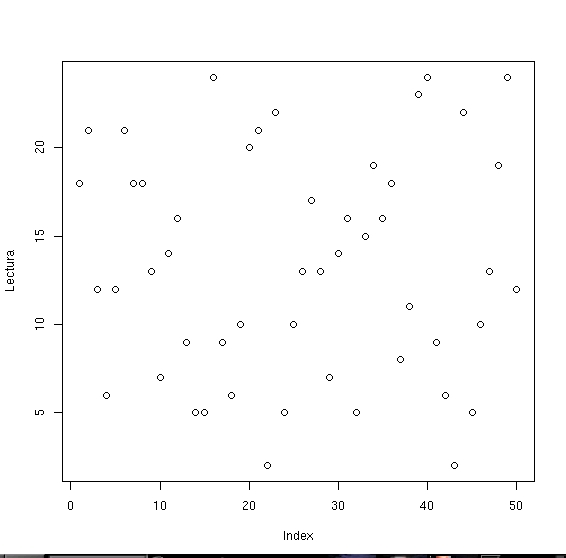
\includegraphics[width=0.49\textwidth]{imagenes/r_plot_1.eps}}
\subfigure[{\tt plot (Lectura, TV)}]{%
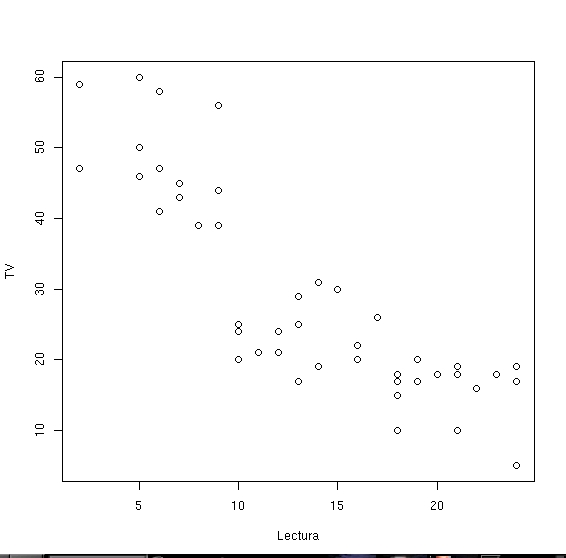
\includegraphics[width=0.49\textwidth]{imagenes/r_plot_2.eps}}
\subfigure[{\tt plot (Ingresos)}]{%
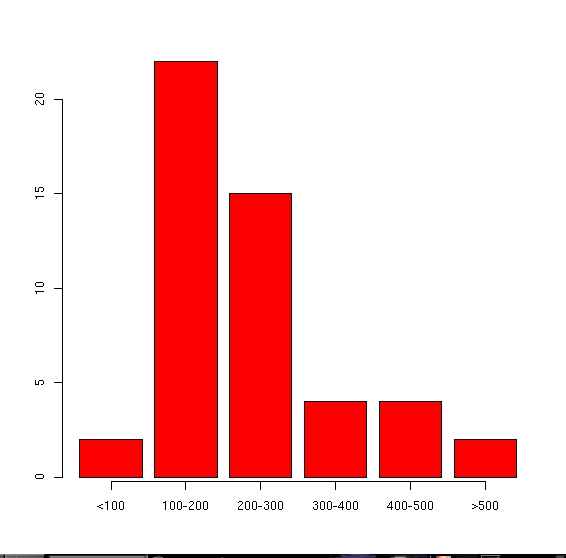
\includegraphics[width=0.49\textwidth]{imagenes/r_plot_3.eps}}
\subfigure[{\tt plot (Ingresos, Habitat)}]{%
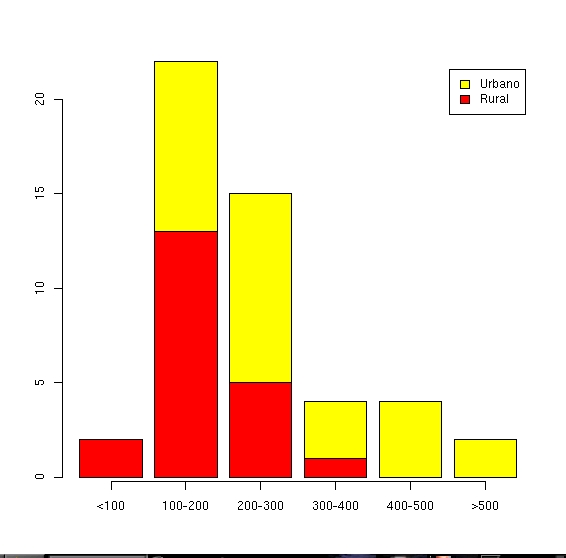
\includegraphics[width=0.49\textwidth]{imagenes/r_plot_4.eps}}
\caption{Las distintas formas de la funci�n {\tt plot()}}
\end{figure}

\index{R!gr�ficas!qqplot@{\tt qqplot()}}

Otras gr�ficas interesantes son  las de comparaci�n de distribuciones,
basadas en  los cuantiles. La funci�n  {\tt qqnorm ()} toma  un vector
num�rico y  lo representa comparando  sus cuantiles con  los cuantiles
te�ricos  (los que  se  esperar�an  en una  muestra  que siguiera  una
distribuci�n normal). La funci�n {\tt  qqline()} a�ade a la gr�fica la
recta que pasa por los cuartiles de los datos y la distribuci�n.

\begin{figure}[hbtp]
\centering
\subfigure[Gr�fico Q-Q para {\tt Lectura}]{%
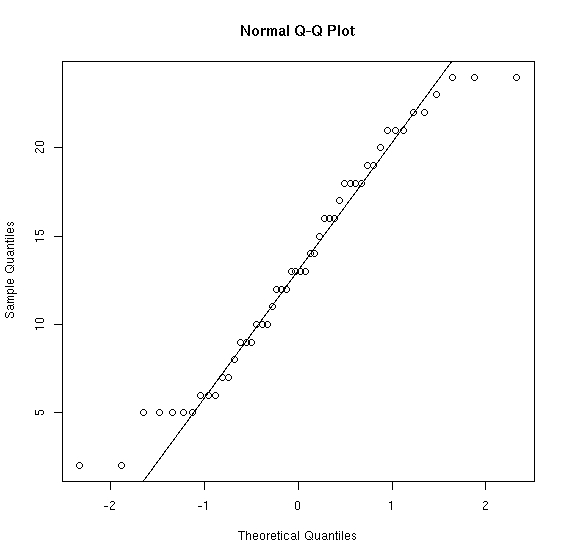
\includegraphics[width=0.49\textwidth]{imagenes/r_qqplot_1.eps}}
\subfigure[Gr�fico Q-Q para {\tt TV}]{%
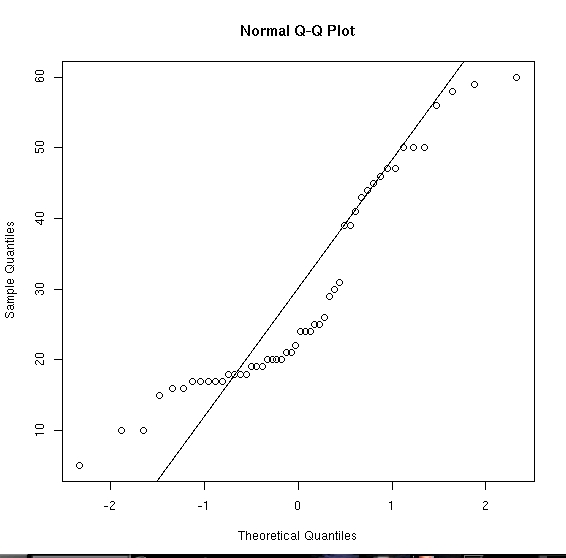
\includegraphics[width=0.49\textwidth]{imagenes/r_qqplot_2.eps}}
\caption[Gr�ficos Q-Q para dos variables]%
{Gr�ficos Q-Q para dos variables, una que se comporta como una
normal y otra que no}
\end{figure}

\index{R!gr�ficas!image@{\tt image()}}
\index{R!gr�ficas!contour@{\tt contour()}}
\index{R!gr�ficas!persp@{\tt persp()}}

Para  representar  matrices puedes  optar  por  ver sus  valores  como
im�genes. La  funci�n {\tt image()} lo  hace a modo de  una rejilla de
rect�ngulos de  diferentes colores  para representar  el valor  de las
celdas. Para  verlo en forma de  contorno usa {\tt contour()},  y para
verlo en perspectiva utiliza {\tt persp()}.

\begin{figure}[htbp]
\centering
\subfigure[{\tt image(volcano)}]{%
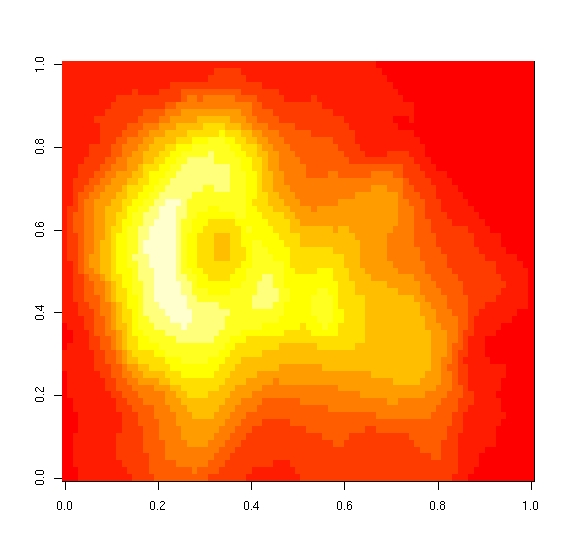
\includegraphics[width=0.49\textwidth]{imagenes/r_image.eps}}
\subfigure[{\tt contour(volcano)}]{%
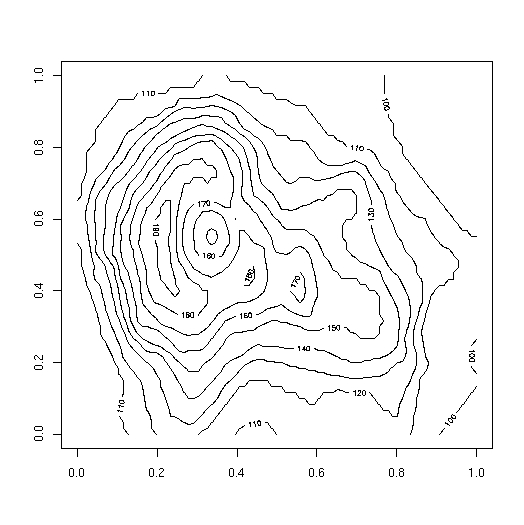
\includegraphics[width=0.49\textwidth]{imagenes/r_contour.eps}}
\subfigure[{\tt persp(volcano)}]{%
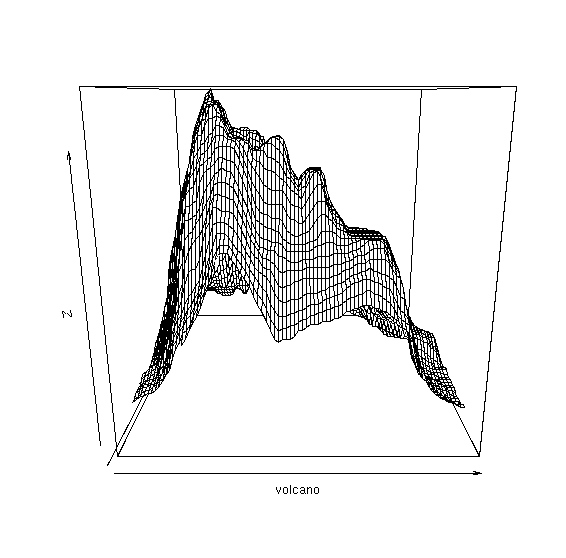
\includegraphics[width=0.49\textwidth]{imagenes/r_persp.eps}}
\subfigure[{\tt Gr�fica de sectores para la Edad}]{%
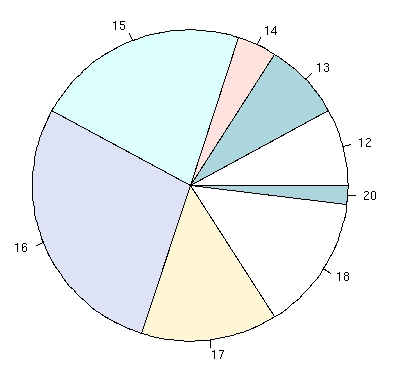
\includegraphics[width=0.49\textwidth]{imagenes/r_pie.eps}}
\caption[Gr�ficas para  representar matrices]%
{Gr�ficas para  representar matrices. El objeto  {\tt volcano}
lo obtenemos al ejecutar {\tt data(volcano)}}
\end{figure}

Los gr�ficos de sectores te dan una impresi�n clara a primera vista de
los  porcentajes que  tienen cada  ``clase'' en  una clasificaci�n  de
datos.  Por ejemplo  para ver  los porcentajes  de personas  seg�n las
edades representamos en un gr�fico de sectores el n�mero de individuos
que tiene cada edad. Una forma de hacerlo (seguramente no es la mejor)
ser�a:

\index{R!gr�ficas!de sectores}

\begin{verbatim}
> pie (tapply (Edad, fedad, length))
\end{verbatim}

\index{R!gr�ficas!pie@{\tt pie()}}

%Autor: miguev
%miguev: 15

\chapter{Yacas}
\label{yacas.tex}

\index{Yacas}
\index{cálculo simbólico}

En  este tema  aprenderás a  utilizar el  programa Yacas  para relizar
cálculos simbólicos.  Este tipo de  cálculos resulta de  gran utilidad
puesto que  funciona de  la misma  forma que harías  tú mismo  a mano,
operando con expresiones matemáticas sin calcular el valor numérico de
cada expresión. 



\section{¿Qué es Yacas?}

Yacas  es un  Sistema  de  Álgebra Computacional  (en  inglés CAS,  de
\index{CAS}
\index{Álgebra Computacional}
Computer  Algebra  System) de  propósito  general  fácil de  usar.  Un
Sistema  de Álgebra  Computacional (SAC)  es un  programa que  permite
manipulaciones simbólicas sobre expresiones matemáticas, reduciendo el
tiempo necesario  para realizar  cálculos embarazosos  pero triviales.
Esto se hace  no mediante números, sino mediante símbolos,  por lo que
el resultado de una operación con expresiones matemáticas es una nueva
expresión matemática.

Yacas  está  construido  sobre  su  propio  lenguaje  de  programación
diseñado  para  este  propósito,  en  el  que  se  pueden  implementar
fácilmente  nuevos  algoritmos.  Además, incorpora  una  documentación
extensa sobre las funcionalidades que  implementa y los métodos usados
para implementarlas.

Entre las  características que Yacas implementa  encontramos precisión
arbitraria, números racionales,  vectores, números complejos, cálculos
con  matrices  (incluyendo  inversas, determinantes  y  resolución  de
sistemas lineales), derivación, series  de Taylor, resolución numérica
(método  de Newton),  y un  montón más  de algoritmos  no matemáticos.
Tiene  también  soporte  básico   para  polinomios  en  una  variable,
integración de funciones y cálculo tensorial.

En  la  web  del proyecto  Yacas  ({\tt  http://yacas.sourceforge.net}
encontrarás el  código fuente  del programa  y toda  su documentación:
desde  un tutorial  básico hasta  una guía  de programación  en Yacas.
Parte  del  texto de  este  tema  son  traducciones  de trozos  de  la
documentación oficial de Yacas que se distribuye junto con el programa
bajo licencia GPL.



\section{Empezando con Yacas}

Yacas  tiene  un  intérprete  de comandos  que  nos  permite  ejecutar
funciones para probar  lo que queremos programar,  para luego escribir
un script  (un fichero de  comandos a modo  de guión). Para  entrar al
intérprete de Yacas  basta con ejecutar el comando {\tt  yacas} en una
consola  o terminal.  Para  salir del  intérprete  puedes pulsar  {\tt
Control-C}  o bien  ejecutar la  función \verb+Exit();+.  Pulsar  {\tt
Control-C} también  es útil  para detener inmediatamente  la ejecución
del intérprete de Yacas (o de un script escrito para Yacas).

\begin{verbatim}
$ yacas
[editvi.ys] [unix.ys] 
True;
Numeric mode: "Gmp"
To exit Yacas, enter  Exit(); or quit or Ctrl-c. Type ?? for help.
Or type ?function for help on a function.
Type 'restart' to restart Yacas.
To see example commands, keep typing Example();
In>
\end{verbatim}

También  existe una  interfaz gráfica  llamada Proteus.  Si la  tienes
instalada  deberías   poder  iniciarla  ejecutando  el   comando  {\tt
proteusworksheet}. Esta utilidad te proporciona un entorno  más cómodo
e integrado  en el  que  puedes  probar código  en  el intérprete e ir
escribiendo un script en el editor que incluye.

\begin{figure}[hbt]
\centering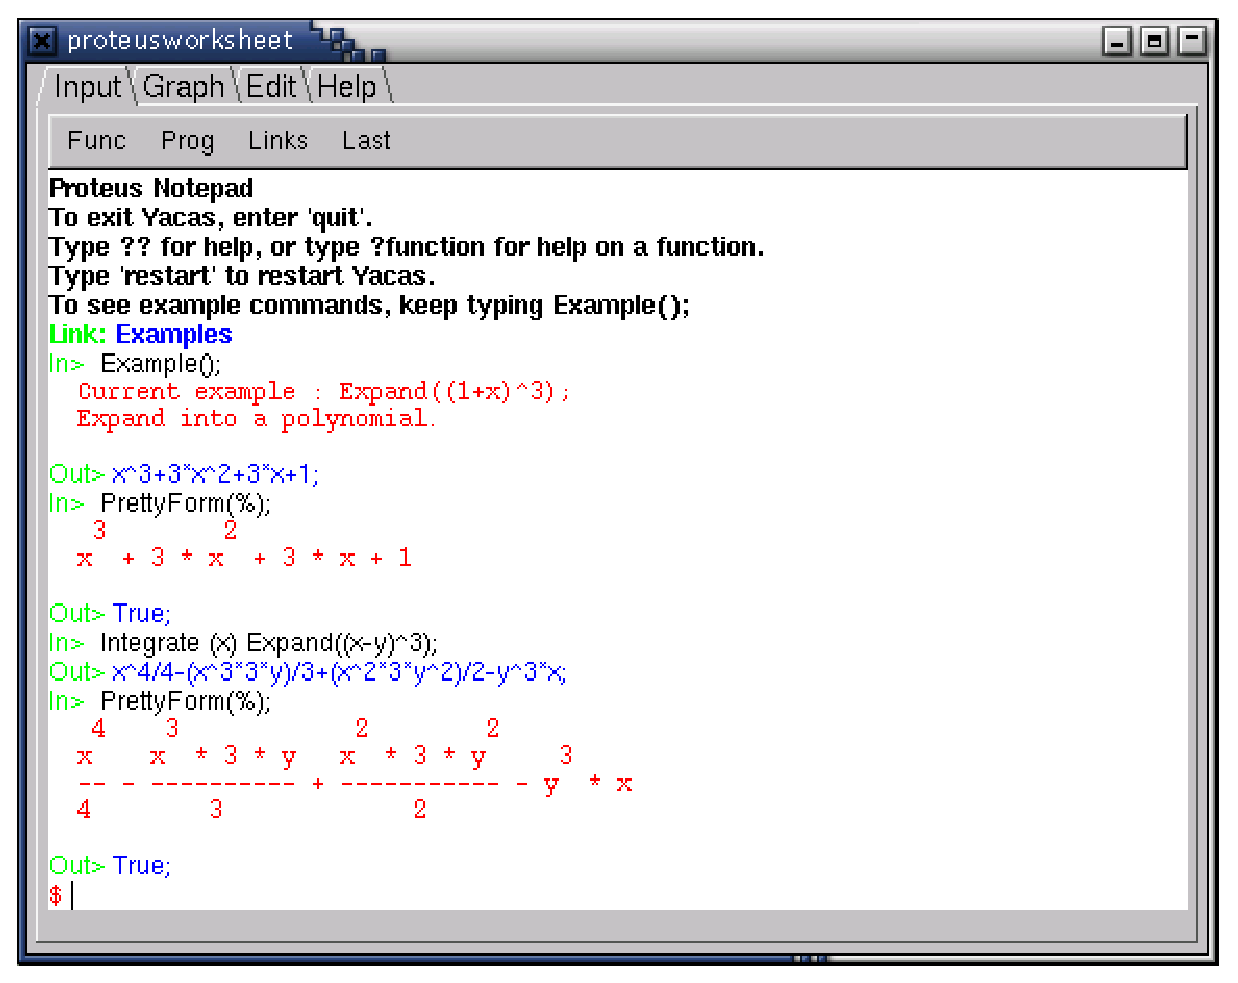
\includegraphics[width=\textwidth]{imagenes/proteus.eps}
\index{proteus}
\index{Yacas!proteus}
\caption{Proteus, interfaz gráfica para Yacas}
\end{figure}

La última línea (\verb+In>+) es el prompt de entrada de Yacas, que nos
indica que  el intérprete está  esperando nuestras órdenes.  Todas las
órdenes de Yacas deben terminar con un punto y coma (\verb+;+), aunque
el intérprete suele  añadirlo si no lo ponemos. Sin  embargo a la hora
de programar en  Yacas veremos que el punto y  coma hay que escribirlo
siempre,  de modo  que es  mejor acostumbrarse  a ponerlo  para evitar
posteriores dolores de cabeza.

Para ir abriendo  el apetito sigue la sugerencia de  Yacas: ejecuta la
función  \verb+Example();+ varias  veces. Por  supuesto no  tienes que
teclear el comando todas las veces, ya que Yacas cuenta con edición de
línea. Esto  incluye que todos los  comandos que ejecutes en  Yacas se
almacenarán  en un  historial, y  para repetirlos  puedes recuperarlos
pulsando  la  tecla  de  cursor hacia  arriba.  Este  historial  queda
guardado en  el fichero \verb+~/.yacas_history+. Veamos  la salida que
produce Yacas tras varias ejecuciones de \verb+Example();+.

\begin{verbatim}
In> Example();
Current example : 40!;

Simple factorial of a number.

Out> 815915283247897734345611269596115894272000000000;
In> Example();
Current example : D(x)Sin(x);

Taking the derivative of a function (the derivative of Sin(x) with
respect to x in this case).

Out> Cos(x);
In> Example();
Current example : Taylor(x,0,5)Sin(x);

Expanding a function into a taylor series.

Out> x-x^3/6+x^5/120;
In> Example();
Current example : Integrate(x,a,b)Sin(x);

Integrate a function.

Out> Cos(a)-Cos(b);
In> Example();
Current example : Solve(a+x*y==z,x);

Solve a function for a variable.

Out> (z-a)/y;
In> Example();
Current example : Limit(x,0)Sin(x)/x;

Take a limit.

Out> 1;
\end{verbatim}

En cualquier momento puedes acceder  a la documentación de una función
ejecutando la función  precedida por un signo  de interrogación, p.ej.
\verb+?IsFreeOf+. Un detalle  importante de Yacas es  que, como muchos
lenguajes del mundo de Un*x, es sensible a las mayúsculas; esto es, no
es lo mismo \verb+esto+ que \verb+Esto+ ni que \verb+eSTO+.

Estos ejemplos ilustran  lo fácil que es obtener  buenos resultados en
cálculos  simbólicos  con  Yacas.  Sin  embargo  es  probable  que  el
resultado del siguiente ejemplo no te resulte fácil de interpretar:

\begin{verbatim}
In> Integrate(x) Expand((x-y)^3);
Out> x^4/4-(x^3*3*y)/3+(x^2*3*y^2)/2-y^3*x;
\end{verbatim}

la forma en  que Yacas recibe nuestra orden de  integrar $\int (x-y)^3
\, dx$ no es nada críptica, pero su respuesta no es precisamente fácil
de  leer. Esta  forma de  mostrar  las expresiones  matemáticas es  la
normal  en  Yacas,  pero  no  la única.  Podemos  pedir  a  Yacas  que
muestre  las  expresiones  de  forma más  ``bonita''  con  la  función
\verb+PrettyForm()+.

\index{Yacas!PrettyFrom}

\begin{verbatim}
In> PrettyForm(%)

 4    3            2        2         
x    x  * 3 * y   x  * 3 * y     3    
-- - ---------- + ----------- - y  * x
4        3             2              

Out> True;
\end{verbatim}

El signo \verb+%+ es una referencia que apunta siempre al último valor
devuelto por el intérprete, es decir  lo que aparezca a la derecha del
último \verb+Out>+. Esta referencia sólo está disponible cuando usamos
Yacas  como intérprete  interactivo,  no se  puede  utilizar desde  un
script.

Otras  formas  de mostrar  una  expresión  son  las utilizadas  en  el
lenguaje  de  programación  C  y  en  el  lenguaje  tipográfico  \TeX.
Para  mostrar  una  expresión  de estas  formas  están  las  funciones
\verb+CForm()+  y \verb+TeXForm()+  respectivamente. Fíjate  que estas
funciones  no devuelven  la  expresión  que muestran,  por  lo que  no
podemos  utilizar  la  referencia  \verb+%+ dos  veces  seguidas  para
mostrar  una  expresión  (la  segunda mostraría  la  expresión  lógica
\verb+True+). Por  eso escribimos  \verb+Integrate(x) Expand((x-y)^3)+
en cada línea:

\index{Yacas!CFrom}
\index{Yacas!TeXFrom}

\begin{verbatim}
In> CForm (Integrate(x) Expand((x-y)^3))
Out> "pow(x, 4.) / 4. - ( pow(x, 3.) * 3. * y)  / 3. + ( pow(x, 2.) * 
3. * pow(y, 2.))  / 2. - pow(y, 3.) * x";
In> TeXForm (Integrate(x) Expand((x-y)^3))
Out> "$\frac{x ^{4}}{4}  - \frac{x ^{3} 3 y}{3}  + \frac{x ^{2} 3 y ^{
2}}{2} - y ^{3} x$";
\end{verbatim}

La función \verb+CForm()+ devuelve la expresión escrita en lenguaje C,
de forma que  podemos incluirla en el  código de un programa  en C. La
función \verb+TeXForm()+ devuelve la  expresión escrita en el lenguaje
tipográfico  \TeX, de  forma  que podemos  incluirla  en un  documento
escrito en  \TeX~ o \LaTeX.  Por ejemplo,  este libro está  escrito en
\LaTeX, lo  que me  permite incluir la  salida de  \verb+TeXForm()+ en
este  mismo párrafo  con  sólo copiar  y pegar.  De  esta forma  puedo
escribir: $$\int  (x-y)^3 \, dx  = \frac{x  ^{4}}{4} - \frac{x  ^{3} 3
y}{3} + \frac{x ^{2} 3 y ^{2}}{2} - y ^{3} x$$

En ocasiones nos  interesa conocer el valor numérico  de una expresión
determinada, y posiblemente sólo nos interese un número determinado de
decimales.  Yacas  es un  lenguaje  de  precisión arbitraria,  lo  que
significa que puedes  pedirle toda la precisión que  quieras, pero ten
cuidado no le pidas demasiada precisión  si tu máquina no es realmente
potente.

La función \verb+Precision()+ establece  el número de cifras decimales
con  las  que se  aproximarán  los  valores. Estas  aproximaciones  se
realizan con  la función  \verb+N()+, que  además permite  saltarse la
precisión establecida por \verb+Precision()+ pasándosela como segundo
parámetro. En el siguiente ejemplo se ilustra esto:

\index{Yacas!presición}

\begin{verbatim}
In> alpha := Sqrt (Pi ())
Out> Sqrt(3.1415926535897932384626433832795028841971694);
In> Precision (2);
Out> True;
In> N (alpha)
Out> 1.77;
In> Precision (20);
Out> True;
In> N (alpha)
Out> 1.77245385090551602729;
In> N (alpha, 50)
Out> 1.77245385090551602729816748334114518279754945629866;
\end{verbatim}

Normalmente  no hay  problema  por  pedirle a  Yacas  unos cientos  de
dígitos de precisión, pero siempre que  vayas a trabajar con números o
precisiones enormes recuerda que el tiempo necesario para los cálculos
aumentará rápidamente.



\section{Variables y funciones}

\index{Yacas!variables}
\index{Yacas!funciones}

En Yacas se entiende por variable un objeto al que se puede asignar un
valor.  Las variables  pueden  llamarse como  quieras  siempre que  el
nombre  empiece  por  una  letra  y continúe  con  letras  y  números.
Para  asignar un  valor  a  una variable  se  utiliza  el operador  de
asignación \verb+:=+ en lugar de \verb+=+ (este último se utiliza como
comparador). En cualquier momento puedes  ver el valor de una variable
tecleando su nombre como si fuera  un comando de Yacas, y esto también
es válido en un script. Asignaciones válidas son:

\begin{verbatim}
In> n := 10;
Out> 10;
In> m := n!;
Out> 3628800;
In> n
Out> 10;
In> m
Out> 3628800;
\end{verbatim}

Si en algún momento quieres que una variable pierda su valor no tienes
más que ``limpiarla'' con la función \verb+Clear()+:

\begin{verbatim}
In> m
Out> 3628800;
In> Clear (m);
Out> True;
In> m
Out> m;
\end{verbatim}

Las funciones  son como las  variables, con  el añadido de  que pueden
depender de una o más  variables. Además con Yacas podemos sobrecargar
una función, esto  es, definir dos funciones con el  mismo nombre pero
distinto número de  variables de forma que se evalúe  una u otra según
el número de parámetros que reciba.

Como ejemplo definimos la función \verb+Area+ de dos formas: si recibe
un parámetro  devuelve el área  del círculo con  el radio igual  a ese
parámetro, pero si recibe dos parámetros devuelve el área de la elipse
que tenga esos dos parámetros como radios.

\begin{verbatim}
In> Area (r) := Pi () * r^2;
Out> True;
In> Area (a, b) := Pi () * a * b;
Out> True;
In> Area (3);
Out> 28.2743338823;
In> Area (3, 5);
Out> 47.1238898035;
\end{verbatim}

Al definir  una función, Yacas no  evalúa la parte de  la derecha sino
que se asigna  como expresión simbólica. Esto puede  no interesarte en
casos como el que ilustra el siguiente ejemplo:

\begin{verbatim}
In> f(x) := x^5;
Out> True;
In> g(x) := D(x) f(x);
Out> True;
In> g(x)
Out> 5*x^4;
In> g(2)
Out> 5*x^4;
\end{verbatim}

Sería  deseable que  \verb+g(2)+  devolviera el  valor  de la  función
\verb+g(x)+  cuando  \verb+x+  vale  $2$,   pero  no  lo  hace  porque
\verb+g(x)+ almacena la expresión  \verb+5*x^4+ sin ninguna referencia
a la  necesidad de evaluarla en  un valor determinado. Sin  embargo si
indicamos a  Yacas que  evalúe la  expresión antes  de asignarla  a la
función  (mediante  \verb+Eval()+)  podremos  pedirle  que  evalúe  la
función \verb+g(x)+ en valores determinados. Esto que parece un follón
es  en realidad  simple, el  siguiente ejemplo  muestra el  código que
funciona como es de esperar:

\begin{verbatim}
In> g(x) := Eval (D(x) f(x));
Out> True;
In> g(x)
Out> 5*x^4;
In> g(2)
Out> 80;
\end{verbatim}



\section{Listas}

\index{Yacas!listas}

Uno de  los elementos más  importantes del  lenguaje de Yacas  son las
listas, que como era de esperar son grupos de objetos ordenados. Yacas
representa las listas  con sus elementos entre llaves  y separados por
comas.  Los  vectores  son  listas,  y  las  matrices  son  listas  de
listas. De  hecho, cualquier expresión  matemática en Yacas  puede ser
transformada en una  lista. Para acceder a los elementos  de una lista
puedes  usar la  notación habitual  en los  corchetes, y  no sólo  con
números  sino también  con secuencias  de ellos.  Los elementos  de la
lista pueden ser cualquier tipo de objetos.

\begin{verbatim}
In> lista := {a, b, c, d, e, f};
Out> {a,b,c,d,e,f};
In> lista[2];
Out> b;
In> lista[2 .. 4];
Out> {b,c,d};
\end{verbatim}

Fíjate  que los  espacios a  ambos  lados del  operador \verb+..+  son
necesarios  para distinguir  estos puntos  de los  que podrían  formar
parte de un número.

También puedes  indexar una lista  con palabras, no sólo  con números.
Esto  te permite  tener pequeñas  bases de  datos en  forma de  listas
asociativas con parejas clave -- valor.

\begin{verbatim}
In> boy := {};
Out> {};
In> boy["nombre"] := "Eric";
Out> True;
In> boy["apellido"] := "Cartman";
Out> True;
In> boy["edad"] := 7.34;
Out> True;
In> boy["educado"] := False;
Out> True;
In> boy
Out> {{"educado",False},{"edad",7.34},{"apellido","Cartman"},
{"nombre","Eric"}};
\end{verbatim}



\section{Álgebra Lineal}

\index{Yacas!Álgegra Lineal}
\index{Yacas!matrices}
\index{Yacas!vectores}

Los  vectores  de  dimensión  fija  se  representan  mediante  listas.
La  lista  \verb+{1,2,3}+ es  el  vector  $(1,2,3)$. Las  matrices  se
representan  como vectores  de  vectores. Dado  que  los vectores  son
realmente listas, sus elementos pueden  asignarse igual que los de las
listas:

\begin{verbatim}
In> l := ZeroVector (3);
Out> {0,0,0};
In> l;
Out> {0,0,0};
In> l[2] := 2;
Out> True;
In> l;
Out> {0,2,0};
\end{verbatim}

Yacas puede multiplicar vectores, matrices y números del modo usual en
álgebra lineal:

\begin{verbatim}

In> v := {1, 0, 0, 0}
Out> {1,0,0,0};
In> E4 := { {0, u1, 0,  0}, \
In>         {d0, 0, u2, 0}, \
In>         {0, d1, 0,  0}, \
In>         {0, 0,  d2, 0} }
Out> {{0,u1,0,0},{d0,0,u2,0},{0,d1,0,0},{0,0,d2,0}};
In> PrettyForm (%)

/                             \
| ( 0 )  ( u1 ) ( 0 )  ( 0 )  |
|                             |
| ( d0 ) ( 0 )  ( u2 ) ( 0 )  |
|                             |
| ( 0 )  ( d1 ) ( 0 )  ( 0 )  |
|                             |
| ( 0 )  ( 0 )  ( d2 ) ( 0 )  |
\                             /

Out> True;
In> CharacteristicEquation (E4, x)
Out> x^4-x*u2*d1*x-u1*d0*x^2;
In> Expand (%, x)
Out> x^4-(u2*d1+u1*d0)*x^2;
In> PrettyForm (%)

 4                            2
x  - ( u2 * d1 + u1 * d0 ) * x 

Out> True;
In> v  +  E4 * v  +  E4 * E4 * v  +  E4 * E4 * E4 * v
Out> {u1*d0+1,d0+(d0*u1+u2*d1)*d0,d1*d0,d2*d1*d0};
In> PrettyForm (%)

/                                 \
| u1 * d0 + 1                     |
|                                 |
| d0 + ( d0 * u1 + u2 * d1 ) * d0 |
|                                 |
| d1 * d0                         |
|                                 |
| d2 * d1 * d0                    |
\                                 /

Out> True;
\end{verbatim}

La librería estándar de Yacas incluye también cálculo del determinante
y  la inversa  de una  matriz,  autovectores y  autovalores (en  casos
simples) y resolución de sistemas  de ecuaciones lineales del tipo $Ax
= b$ donde $A$ es una matriz y $x$ y $b$ son vectores.



\section{Control de flujo}

\index{Yacas!control de flujo}

El lenguaje de  Yacas incluye algunas construcciones  y funciones para
el control  de flujo. Para ello  necesitas saber también que  Yacas te
permite agrupar bloques  de instrucciones de forma  que aparezcan como
una sola instrucción. Para ello simplemente encierra las instrucciones
del  bloque entre  corchetes  (\verb+[+ y  \verb+]+),  o bien  utiliza
la  función \verb+Prog()+  pasándole las  instrucciones separadas  por
\verb+;+.

Para  los  bucles  disponemos  de  las  funciones  \verb+ForEach()+  y
\verb+While()+. La  función \verb+ForEach (x, list) body+  ejecuta  el
bloque de  instrucciones \verb+body+  para cada  elemento de  la lista
\verb+list+ asignando el valor de cada elemento a la variable \verb+x+
en cada interación. La función \verb+While (predicate) body+ repite el
bloque \verb+body+  hasta que  la condición  \verb+predicate+ devuelva
\verb+False+.

Para   los  condicionales   está  la   función  
\verb+If (predicate, body1, body2)+,
en la  que  se  ejecuta  el bloque  \verb+body1+  si
\verb+predicate+ devuelve \verb+True+ o ejecuta el bloque \verb+body2+
si \verb+predicate+  devuelve \verb+False+, y en  ambos casos devuelve
el  valor devuelto  por  el  bloque ejecutado.  El  segundo bloque  es
opcional.  Si  llamas  a  \verb+If (predicate,  body1)+  se  ejecutará
el  bloque \verb+body1+  si  \verb+predicate+  devuelve \verb+True+  y
devolverá  el valor  que devuelva  \verb+body1+, o  bien se  devolverá
\verb+False+ si así lo hace \verb+predicate+.

Como ejemplo de control de flujo construimos una lista con los números
enteros pares  de $2$ a  $20$ y calculamos el  producto de los  que no
sean divisibles por $3$. Luego definimos  el factorial de un número de
forma recursiva.

\begin{verbatim}
In> L := {};
Out> {};
In> i := 2;
Out> 2;
In> While (i <= 20) [ \
In>   L := Append (L, i); \
In>   i := i + 2; \
In> ];
Out> True;
In> L;
Out> {2,4,6,8,10,12,14,16,18,20};
In> answer := 1;
Out> 1;
In> ForEach (i, L) [ \
In>   If ( Mod (i, 3) != 0, \
In>     answer := answer * i \
In>   ); \
In> ];
Out> True;
In> answer;
Out> 2867200;
In> Factorial (x) := [ \
In>   If ( IsInteger (x) And x >= 0, \
In>     If (x = 0, 1, \
In>       x * Eval (Factorial (x-1)) ), \
In>   False ); \
In> ];
In> Factorial (5)
Out> 120;
In> Factorial (25)
Out> 15511210043330985984000000;
\end{verbatim}

Una  barra  invertida  \verb+\+  al  final  de  una  línea  indica  al
intérprete de Yacas que la línea  no está terminada, sino que continúa
después  del salto  de carro.  En  este ejemplo  hemos utilizado  esto
descaradamente. Esto se puede utilizar en el intérprete para hacer que
nuestros comandos  sean más cómodos de  leer, pero no es  necesario al
escribir un script.



\section{Gráficas}

\index{Yacas!gráficas}

Yacas incorpora la posibilidad de representar gráficas bidimensionales
utilizando  GNUplot, si  bien  esta capacidad  depende  de que  tengas
instalado también  el programa  GNUplot. Para saber  si tu  versión de
Yacas  tiene soporte  para  GNUplot  fíjate en  la  primera línea  que
imprime el  intérprete cuando arranca, si  aparece \verb+[gnuplot.ys]+
es   que   tu   versión   de   Yacas   soporte   para   gráficas   con
GNUplot\footnote{Esto  era cierto  hasta la  versión 1.0.50  de Yacas,
pero  en el  momento de  escribir esta  nota la  versión 1.0.51  de mi
máquina no  aparece {\tt [gnuplot.ys]}  pero puede hacer  las gráficas
con la función {\tt Plot2D}}.

\begin{verbatim}
$ yacas
[editvi.ys] [gnuplot.ys] [unix.ys]
\end{verbatim}

La función para  representar gráficas es \verb+Plot2D()+  y recibe dos
parámetros: la expresión  (o lista de expresiones)  para representar y
el  intervalo  de  la  variable  en  la  forma  {\tt  valor\_minimo  :
valor\_maximo}.

En anteriores versiones de Yacas, la función para representar gráficas
era \verb+GnuPlot()+ y  recibía cuatro parámetros: el  valor mínimo de
la  variable, el  valor máximo  de la  variable, el  número de  puntos
utilizados para la representación y la función para representar. 

En los  siguientes ejemplos  calculamos el el  polinomio de  Taylor de
orden 5 para la función $\sin(x)$  en el origen y la representamos (en
rojo) junto con la función $\sin(x)$ (en verde).

\begin{figura}{yacas_gnuplot}{0.8}
\caption{Representación gráfica con GNUplot desde Yacas}
\end{figura}

\begin{verbatim}
In> f(x) := Eval (Taylor (x, 0, 5) Sin(x) )
Out> True;
In> Plot2D ({f(x), Sin (x)}, -Pi:Pi)
Out> True;
In> GnuPlot (-Pi(), Pi(), 50, {f(x), Sin(x)})
GnuPlot: created file gnuplot.tmp/gnudata.in1
GnuPlot: created file gnuplot.tmp/gnudata.in2
Out> True;
\end{verbatim}

\section{Programando con Yacas}

\index{Yacas!programación}

Si bien  el intérprete de  Yacas proporciona una interfaz  cómoda para
ejecutar  cálculos, cuando  éstos  se complican  resulta más  práctico
escribir un ``script'' y ejecutarlo  con Yacas. Para hacer un programa
con Yacas escribe en un fichero  la secuencia de comandos que componen
el  programa, incluyendo  definiciones de  funciones. Los  ficheros de
script  de Yacas  suelen tener  tener la  extensión {\tt  .ys} (no  es
obligatorio).  

Para ejecutar  el script simplemente  ejecuta Yacas dándole  el nombre
del fichero como parámetro. La opción {\tt -c} del comando {\tt yacas}
hace que Yacas  no muestre los prompts \verb+In>+  y \verb+Out>+ (útil
para sesiones no interactivas, como el caso de ejecutar un script). El
siguiente ejemplo  muestra como ejecutar  un script en Yacas,  en este
caso el script es el fichero de ejemplo {\tt lagrange.ys}

\begin{verbatim}
$ yacas -c lagrange.ys
\end{verbatim}

\begin{ejemplo}{lagrange.ys}{Script en Yacas que interpola una función}
\index{Yacas!script}
Script en Yacas  que muestra un interpolante de Lagrage  para una nube
de cinco  puntos tomados  de la función  $f(x) =  \frac{1}{1+x^2}$. En
este  ejemplo el  interpolante de  Lagrange  no es  el adecuado,  pero
nuestra intención  no es interpolar  $f(x)$
\end{ejemplo}

Otra   forma  de   ejecutar  un   script  es   desde  el   intérprete,
mediante  las  funciones  \verb+Load()+  y  \verb+Use()+.  La  función
\verb+Load("script.ys")+  lee  el  fichero \verb+script.ys+  y  evalúa
todas  las   expresiones  que   encuentre  en  él.   Siempre  devuelve
\verb+True+.  \verb+Use()+  hace lo  mismo  que  \verb+Load()+ con  la
salvedad de que sólo lee el fichero si no ha sido leído antes por otra
llamada \verb+Load()+ o \verb+Use()+.

Un uso  común de \verb+Use()+ es  cargar un fichero con  funciones con
las que queremos trabajar desde el  intérprete, de modo que no tenemos
que teclear  las funciones  cada vez  ni tampoco  hay que  ejecutar el
script. La función \verb+Load()+ resulta  útil para ejecutar un script
desde el  intérprete cuando queremos hacerlo  varias veces modificando
el script sin salir del intérprete.



\section{Un ejemplo real}

\index{Yacas!ejemplo real}

A continuación  explicamos un ejemplo  del uso  de Yacas ``en  la vida
real'': calcular la sucesión de Sturm  asociada a un polinomio real de
una variable  real. Esta sucesión  se utiliza  en el teorema  de Sturm
para  calcular el  número  de  raíces reales  de  un  polinomio en  un
intervalo de la  recta real. El algoritmo para  calcular esta sucesión
de polinomios no es complicado, pero  por si no lo conoces aquí tienes
una breve explicación:

El algoritmo  de Sturm parte  de un polinomio con  coeficientes reales
$p(x)$  y su  derivada $p'(x)$.  Tomando $f_0(x)  = p(x)$  como primer
polinomio  y $f_1(x)  =  p'(x)$ como  segundo  polinomio, se  realizan
sucesivas divisiones euclídeas utilizando  en cada división el divisor
de la  anterior como dividendo y  el opuesto del resto  de la anterior
como divisor. Al  cabo de un número finito de  iteraciones, en las que
$f_j(x)$ es el resto de la división $j-1$, se obtiene un resto nulo en
la iteración $m+1$.

\begin{eqnarray*}
f_0(x) & = & f_1(x) q_1(x) - f_2(x)          \\
f_1(x) & = & f_2(x) q_2(x) - f_3(x)          \\
& \vdots &                                   \\
f_{m-2}(x) & = & f_{m-1}(x) q_1(x) - f_m(x)  \\
f_{m-1}(x) & = & f_m(x) q_m(x)
\end{eqnarray*}

A  partir de  los polinomios  $f_j$ obtenidos  en estas  divisiones se
construye la sucesión de Sturm asociada a $p(x)$, que viene dada por

$$\left\{\hat{f}_j(x) = \frac{f_j(x)}{f_m(x)}\right\}_{j=0}^{n}$$

El teorema  de Sturm garantiza que  el número de raíces  del polinomio
$p(x)$ en  el intervalo  $[a,b]$ es exactamente  $V(a) -  V(b)$, donde
$V(x_0)$ es el número de variaciones  de la sucesión de Sturm evaluada
en el punto $x_0$,  i.e. el número de cambios de  signo en la suceción
$\left\{   \hat{f}_0(x_0),   \hat{f}_1(x_0),  \ldots,   \hat{f}_m(x_0)
\right\}$.

Para implementar esto en Yacas definimos la función \verb+Sturm()+ que
recibe el polinomio \verb+P+ junto con la variable en la que éste está
expresado \verb+x+  y genera una  lista \verb+L+ con el  polinomio, su
derivada  y los  sucesivos restos  de las  divisiones euclídeas.  Para
ahorrar esfuerzo  computacional acotamos el  número de términos  de la
lista con el grado del polinomio \verb+P(x)+, ya que éste es el número
máximo de divisiones necesarias para encontrar el máximo común divisor
del polinomio y  su derivada. Luego busca el último  polinomio no nulo
en  \verb+L+, que  es  el  máximo común  divisor  del  polinomio y  su
derivada, y construye la sucesión de Sturm en una nueva lista \verb+S+
que  finalmente devuelve  como  valor  de retorno  de  la función.  La
función \verb+Simplify+ simplifica cualquier expresión que reciba.

\begin{ejemplo}{sturm.ys}{Script en Yacas que implementa el algoritmo de Sturm}
Script en Yacas que implementa el algoritmo de Sturm.
\end{ejemplo}

En  el  script  escribimos  esta   función  y  añadimos  los  comandos
necesarios  para  ejecutar  un test.  La  función  \verb+RandomPoly()+
genera un  polinomio aleatorio, lo mostramos  con \verb+PrettyForm()+,
calculamos su sucesión de Sturm y la mostramos con \verb+PrettyForm()+
de nuevo. El resultado de ejecutar el script es el siguiente:

\begin{verbatim}
     3         2            
7 * x  + 10 * x  + 3 * x + 3


/                                          \
|     /           2                      \ |
| 9 * \ -96605 * x  + 73253 * x - 181452 / |
| ---------------------------------------- |
|                 2685619                  |
|                                          |
| 81 * ( -139 * x - 117 )                  |
| -----------------------                  |
|          19321                           |
|                                          |
| 1                                        |
\                                          /
\end{verbatim}

Este ejemplo  real ha sido  extraido del programa presentado  por unos
alumnos como trabajo para  asignatura ``Álgebra Computacional'' que se
imparte en la Facultad de Matemáticas  de la Universidad de La Laguna.
En  teoría  debieron realizar  el  trabajo  utilizando Maple  V,  pero
propusieron al profesor la alternativa  de programarlo en Yacas y éste
aceptó con  curiosidad. El programa  aproxima las raíces reales  de un
polinomio utilizando el  algoritmo de Sturm para aislar  las raíces en
intervalos y aproximándolas  con el método de la  bisección (raíces de
multiplicidad  impar)  o  con  el método  de  cristalización  simulada
(raíces de multiplicidad par). El trabajo fue expuesto en clase y tuvo
la calificación de sobresaliente, el código y las transparencias están
disponibles en {\tt http://www.fmat.ull.es/\~{}miguev/algcomp/}



% M�dulo V:   Programaci�n
% 1. Editores de texto (gvim, xemacs)
% 2. Bash
% 3. GNU Fortran 77
% 4. FreePascal
% 5. GNU C/C++
% 6. Java
% 7. GNU Make
% 8. Depuradores (gdb y ddd)
\part{Programaci�n}
%Autor: miguev && Carlos de la Cruz (frodo@fmat.ull.es)


\chapter{Editores de VI y Emacs}



\section{Joe}


El primer editor  que suele aprenderse en Linux es  {\tt Joe}, por ser
muy sencillo  y r�pido.  Puede usarse  para editar  cualquier fichero,
pero  aqu�  trataremos su  uso  b�sico  para editar  peque�os  textos,
ficheros de  configuraci�n, peque�os  programas. Todos  estos ficheros
pueden editarse con m�s comodidad con editores m�s potentes como Emacs
o VIM pero para ello es  necesario aprender a usarlos primero, lo cual
puede no resultar tan sencillo como aprender {\tt Joe}.

Veremos s�lo un par de comandos  de {\tt Joe}, simplemente como editar
un fichero existente o nuevo, guardarlo sin salir, salir sin guardarlo
y salir guard�ndolo. Para obtener m�s informaci�n sobre otras opciones
del editor existe el comando de ayuda que explicaremos luego.

El  manejo de  {\tt Joe}  se basa  en combinaciones  de teclas  con la
tecla {\tt  Control}. Denotaremos  por {\tt  \flq Ctrl\frq  x y}  a la
combinaci�n de teclas que se obtiene al pulsar la tecla {\tt Control},
seguidamente (sin soltar la primera) pulsar la tecla {\tt x} y despu�s
(soltando las  teclas anteriores) pulsar  la tecla {\tt y}.  Veamos un
r�pido ejemplo del uso de este editor. En un terminal ejecutamos:

\begin{verbatim}
$ joe prueba.txt
\end{verbatim}


Escribimos una frase sencilla, tal como:


\begin{verbatim}
Si algo funciona, no lo toques.
\end{verbatim}

Para guardar el fichero utilizamos la combinaci�n de teclas {\tt \flq
Ctrl\frq k s} y entonces {\tt Joe} nos preguntar� el nombre con el que
queremos guardar el fichero.

\begin{verbatim}
Name of file to save (^C to abort): hola.txt
\end{verbatim}

Si pulsamos ahora  ahora {\tt \flq Ctrl\frq  c} simplemente cancelamos
la orden  de guardar el fichero,  pero no perdemos su  contenido. Para
guardar el  fichero pulsamos  {\tt Enter},  modificando el  nombre del
fichero si lo deseamos. Ahora a�adimos otra l�nea:

\begin{verbatim}
Si algo funciona, no lo toques.
Si algo funciona, y no sabes por qu�, �salo siempre.
\end{verbatim}

Ahora saldremos  del editor {\bf  guardando los cambios},  mediante la
combinaci�n  de  teclas  {\tt  \flq  Ctrl\frq k  x}.  De  esta  manera
volveremos al prompt  del sistema siendo informados de  que el fichero
ha sido guardado.

\begin{verbatim}
File prueba.txt saved.
$
\end{verbatim}

Como �ltima maniobra, abrimos de  nuevo el fichero, borramos la �ltima
l�nea y salimos sin guardar los cambios.


\begin{verbatim}
$ joe prueba.txt
\end{verbatim}

Boramos la �ltima l�nea como har�amos  en el {\tt edit} del {\tt DOS},
y pulsamos {\tt  \flq Ctrl\frq c} para salir sin  guardar los cambios.
El editor  nos pedir� confirmaci�n  antes de salir.  Podemos responder
que s� queremos salir pulsando {\tt y}, o por el contrario cancelar la
maniobra pulsando  {\tt n}  o {\tt  \flq Ctrl\frq  c}. Decimos  que s�
({\tt y}) y volvemos al prompt del sistema.

\begin{verbatim}
Lose changes to this file (y,n,^C)? 
File hola.txt not saved.
$
\end{verbatim}

Esto es lo m�nimo  que debemos saber para editar con  {\tt Joe}, y con
esto nos conformaremos  aqu� pues en lo sucesivo  aprenderemos a hacer
operaciones m�s avanzadas con otros editores. Para conocer sobre otras
opciones  de  este editor,  se  puede  utilizar  la opci�n  {\tt  \flq
Ctrl\frq k h}.

      

\section{Emacs }


{\tt Emacs}, junto con {\tt VI},  ha sido uno de los primeros editores
de  texto para  UNIX. A  pesar  de visualmente  presentar un  interfaz
similar al  de un  editor de  texto corriernte,  como podr�a  ser {\tt
joe},  el {\tt  edit} de  MS-DOS, o  similar, lo  cierto es  que tiene
much�simas posibilidades que uno no atribuir�a a un editor de texto en
modo consola. Por  ejemplo, el indentado autom�tico  de c�digo Pascal,
Java, C, o cualquier lenguaje para  el que haya escrito un m�dulo para
Emacs de  asistencia a  la programaci�n,  nos ofrece  posibilidades de
trabajar con  CVS, enviar correo  electr�nico, y un largo  etc�tera de
posibilidades. Como an�cdota cabe contar,  para que se hagan una idea,
el manual de GNU Emacs, en formato ASCII ocupa cerca de 1.1 MB.


Hablemos de c�mo manejarse con los  men�s de Emacs. Existen cientos de
combinaciones de teclas en Emacs que nos permiten hacer cualquier cosa
sin  ver  un  men�.  Los  usuarios  expertos  de  Emacs  valoran  esta
posibilidad, pues a la hora de  escribir con prisas, un men� puede ser
algo muy inc�modo.  Pero para ustedes que  est�n empezando, recuerden:
la tecla {\tt \flq F10\frq } es su amiga.

La tecla {\tt \flq F10\frq } nos da acceso a todos los men�s de Emacs,
menu archivo, edici�n, cambio entre  las distintas ventanas de edici�n
de texto, etc.

Empezemos viendo como editar un fichero de texto b�sico. En la consola
ponemos:

\begin{verbatim}
$ emacs prueba.c
\end{verbatim}

y escribimos un programa com�n y corto:

\begin{verbatim}
#include <stdio.h>
int
main()
{
  printf("\nHola Mundo\n\n");
}
\end{verbatim}

Como podemos apreciar,  Emacs hace retroceder el cursor  al cerrar los
corchetes y los par�ntesis, para  indicarnos d�nde los abrimos y tener
una  referencia de  cu�les quedan  a�n  por cerrar.  Probemos ahora  a
guardar  nuestro peque�o  programa  C. Para  ello  pulsamos {\tt  \flq
F10\frq }  y una vez  pulsada {\tt \flq F10\frq  } vemos que  la tecla
{\tt B} nos dar�a acceso al men� buffers (que no son otra cosa que las
distintas ventanas que tenemos abiertas),  la {\tt F} nos dar�a acceso
al men� {\tt  files} (el cual hace pr�cticamente lo  mismo que el men�
archivo de  cualquier editor de texto,  etc... y la tecla  {\tt C} nos
dar�a  acceso, si  las  tenemos instaladas,  a  las posibilidades  que
ofrece  emacs para  la  edici�n de  c�digo en  C.  Como s�lo  queremos
guardar,  pulsamos despu�s  de {\tt  \flq F10\frq  }, {\tt  S}. Ya  lo
tendr�amos guardado.  Otra cosa muy importante,  en cualquier programa
es saber  salir. Esto se  hace con  {\tt \flq F10\frq  }, {\tt F}  y a
continuaci�n la tecla {\tt S}. Nos  pregunta, si no lo hemos hecho ya,
que  si deseamos  guardar. Escribimos  {\tt yes}  (hay que  escribirlo
entero)  o  {\tt no},  y  a  continuaci�n  nos pregunta  si  realmente
queremos salir,  a lo cual ahora  s�, responderemos {\tt y}  para {\tt
s�} o {\tt n} para {\tt no}.


Desplaz�ndonos por el texto:

Emacs es famoso por sus innumerables combinaciones de teclas para realizar
cualquiera de las operaciones que nos ofrece. Algunas de las combinaciones
de teclas para movernos c�modamente por nuestros documentos son:
\begin{verbatim}

Alt + f : Sit�a el cursor al principio de la palabra siguiente.
Alt + b : Sit�a el cursor al principio de la palabra anterior.
Ctrl + a : Sit�a el cursor al principio de la l�nea actual.
Ctrl + e : Sit�a el cursor al final de la l�nea actual.
Alt + a : Retrocede el cursor hasta el principio de la frase.
Alt + e : Avanza el cursor hasta el final de la frase.
Home(Inicio): Nos permite situarnos al principio del "buffer".
End(Fin): Nos permite situarnos al final del "buffer".
Ctrl + l: Sit�a el cursor justo al principio de la l�nea del medio de la
	  pantalla

\end{verbatim}

Algunas teclas para eliminar texto:

\begin{verbatim}

Alt + d : Elimina la palabra que sigue al cursor.
Alt + delete(supr) : Elimina la palabra anterior al cursor.
Ctrl + k : Elimina la l�nea actual entera.
Alt + k : Elimina la frase siguiente
Ctrl x + BackSpace : Elimina la frase anterior

\end{verbatim}





Hay que a�adir un truco bastante �til que es la combinaci�n de teclas
Ctrl + u, la cual nos permite repetir cualquier comando n veces.

Por ejemplo, si quisi�ramos avanzar 24 palabras, utilizar�amos la secuencia
de teclas:

"Ctrl U" "24" "Alt + f"



Otra funci�n  muy b�sica tambi�n  es la  de buscar y  reemplazar texto.
Esto puede hacerse  c�modamente con la combinaci�n  {\tt \flq Ctrl\frq
-s}, dejando  pulsado la  tecla {\tt \flq  Control}\frq y  pulsando la
{\tt s}, y a continuaci�n poniendo que queremos buscar y pulsando {\tt
Enter}.  Una  vez  encuentre  la primera  coin\-ci\-den\-cia,   puede
seguir busc�ndose el  mismo patr�n  pulsando de  nuevo simplemente  {\tt \flq
Ctrl\frq -s}.

Podemos saber  en todo momento  qu� estamos haciendo fij�ndonos  en la
l�nea inferior de la pantalla de Emacs.

Para  reemplazar  trozos  de  texto, cosa  tambi�n  de  supervivencia,
podemos hacerlo f�cilmente de la siguiente forma:

\begin{enumerate}
\item Pulsamos \flq F10\frq .
\item Pulsamos la S, que corresponde al men� Search.
\item Nos sale el siguiente men�:
\end{enumerate}

\begin{verbatim}
Possible completions are:
S==\frq Search...                      R==\frq Regexp Search...
B==\frq Search Backwards...            0==\frq Regexp Search Backwards...
1==\frq Repeat Search                  2==\frq Repeat Regexp
3==\frq Repeat Backwards               4==\frq Repeat Regexp Backwards
5==\frq Bookmarks                      F==\frq Find Tag...  (M-.)
Q==\frq Query Replace...  (M-%)        6==\frq Query Replace Regexp...
\end{verbatim}

Pulsamos {\tt Q} y nos dice:

{\tt Query  replace:} donde escribiremos  lo que queremos  buscar para
ser reemplazado, y pulsamos {\tt Enter}.

Luego,  emacs  nos   pregunta:  {\tt  query  replace   with:  }  donde
escribiremos el  texto con  el cual  queremos sustituir,  y pulsaremos
enter.

En este  men�, encontramos  tambi�n una serie  de comandos,  como {\tt
query  regexp},  {\tt  query  replace regexp},  etc.,  que  aunque  no
entraremos en ellos,  son muy interesantes, pues  nos permiten buscar,
no  ya patrones  de  texto concretos,  sino un  tipo  de b�squeda  m�s
avanzada por  medio de  expresiones regulares (regular  expressions en
ingl�s), esto es,  ``todas las palabras que empiecen por  c y terminen
por j''  o ``todas  las may�sculas cambiarlas  por min�sculas''  en el
caso de {\tt query replace regexp}.

Insertando un fichero de texto en nuestro documento:

Para  los amantes  del Cut  \& Pasting  (un deporte  muy extendido  en
algunos c�rculos de programadores), aqu� va un comando que nos permite
introducir un documento de texto dentro de otro:

Pulsamos las teclas "Ctrl x", seguidas de la letra "i", para insertar un
fichero en la posici�n actual del cursor. Entonces, en la l�nea de comandos
de emacs, aparecer� el directorio actual. 

Escribimos la ruta completa al archivo y aparecer� en la posici�n actual
del cursor.




\section{VI y VIM}


{\tt VI} es un editor de texto visual, de pantalla completa, basado en
el editor de  l�nea {\tt ex}. Es  un editor poco intuitivo  y con mala
prensa entre los estudiantes que dan sus primeros pasos en UNIX/Linux,
pero por otra parte es el  editor favorito de los usuarios avanzados y
de muchos programadores. Es adem�s un editor que se puede encontrar en
cualquier sistema UNIX, desde antiguas  estaciones Sun Solaris o HP-UX
hasta  las  m�s  recientes  distribuciones  de  GNU/Linux  o  FreeBSD,
OpenBSD, etc.  {\tt VI} es adem�s  un editor muy potente,  que permite
hacer  complicadas  operaciones en  grandes  ficheros  con unos  pocos
comandos, por  lo que  su aprendizaje  puede ahorrarnos  mucho tiempo.
Otra ventaja de {\tt VI} es que al ser tan corriente suele encontrarse
incluso en disquetes de rescate. L�gicamente poco se puede rescatar si
no  se sabe  manejar  el  �nico editor  disponible  en  un momento  de
emergencia. Pero  el manejo de {\tt  VI} es realmente inc�modo  si nos
enfrentamos  a la  versi�n cl�sica.  Por ejemplo  no podemos  usar los
cursores  para  movernos  por  el  texto,  debemos  pasar  al  llamado
``modo comando'' y utilizar letras para movernos.

En este  curso utilizaremos el  editor {\tt VIM}. {\tt  VIM} significa
``{\bf V}i {\bf IM}proved''  (``{\bf VI M}ejorado''), y como
su nombre  indica es un  clon (muy)  mejorado del cl�sico  editor {\tt
VI}. {\tt VIM}  es bastante m�s amigable que {\tt  VI}, ya que permite
un uso m�s intuitivo (p.ej. los cursores y otras teclas para moverse).


Lo primero  que debe aprenderse con  {\tt VIM} es la  filosof�a de los
dos modos de  trabajo: el modo {\tt comando} y  el modo {\tt edici�n}.
El  modo comando  se utiliza  s�lamente  para dar  �rdenes al  editor,
decirles que haga cosas como borrar  una l�nea, buscar un patr�n, ir a
una determinada  l�nea, guardar el  fichero, salir, etc. El  modo {\tt
edici�n} se  utiliza s�lamente para  escribir texto en el  fichero. Es
muy importante familiarizarse con esta filosof�a de funcionamiento, ya
que  resulta imprescindible  para  cualquier operaci�n  que se  quiera
realizar con {\tt VIM}.

Para ejecutar este editor el comando es: 

\begin{verbatim}
$ vi
\end{verbatim}

Aunque  conserva el  nombre de  {\tt VI}  estamos trabajando  con {\tt
VIM}. Este comando admite varias opciones  que se le pueden pasar como
par�metros, p.ej. el nombre del fichero que queremos editar:


\begin{verbatim}
$ vi fichero
\end{verbatim}

{\tt  VIM} comienza  siempre  en modo  {\tt  comando}, preparado  para
realizar operaciones  sobre el  fichero. Una  de estas  operaciones es
pasar al modo {\tt edici�n} pulsando la tecla {\tt i} (Insertar). Para
pasar del modo {\tt edici�n} al como {\tt comando} basta con pulsar la
tecla de  escape, que llamaremos  {\tt \flq ESC\frq }.  A continuaci�n
vamos a editar  un peque�o fichero de prueba  para familiarizarnos con
sus comandos b�sicos.

Comenzamos invocando al editor desde la l�nea de comandos:


\begin{verbatim}
$ vi prueba.txt
\end{verbatim}

Veremos que en la �ltima l�nea de la consola aparece lo siguiente:

\begin{verbatim}
"prueba.txt" [New File]                                        0,0-1 All
\end{verbatim}

Esta  l�nea es  la {\tt  barra de  estado} del  editor. Es  aqu� donde
teclearemos  algunos comandos  y  donde  aparecer� cierta  informaci�n
como el modo en el  que estamos, la  l�nea y columna en la que estamos,
el porcentaje del documento en el que estamos, etc.


A  continuaci�n pulsamos  la tecla  {\tt i}  para pasar  al modo  {\tt
edici�n}. Observamos que la barra de estado se muestra diferente:


\begin{verbatim}
-- INSERT --                                                     0,1 All
\end{verbatim}

 Tecleamos por ejemplo lo siguiente: 

\begin{verbatim} Lo peque�o es bello.  \end{verbatim}

Cuando tenemos algo  escrito, pulsamos {\tt \flq ESC\frq  } para pasar
al modo {\tt comando}. Entonces tecleamos la orden {\tt :w} y pulsamos
{\tt \flq  Enter\frq }. Veremos como  la orden {\tt :w}  aparece en la
barra  de estado  mientras  la  tecleamos, y  luego  al ejecutarla  se
muestra informaci�n sobre el resultado, en este caso informaci�n sobre
el fichero que acabamos de guardar.

\begin{verbatim}
"prueba.txt" [New] 1L, 21C written                              1,20 All
\end{verbatim}

Pasamos nuevamente al modo {\tt  edici�n} pulsando {\tt a} (observamos
la diferencia con pulsar {\tt i}) y continuamos escribiendo:

\begin{verbatim}
   ---
   Lo peque�o es bello.
   ---
   La  medida de programar es programar sin medida.
   ---
   Software is like sex, it's better when it's free.
   ---
\end{verbatim}

Observamos como podemos movernos libremente  por el texto en modo {\tt
edici�n} utilizando los cursores, las  teclas de Inicio, Fin, Av. Pag,
Re. Pag., etc. Esto no puede  hacerse en el {\tt VI} cl�sico. Volvemos
a guardar el fichero con la orden {\tt :w}.

Ahora pensemos  que queremos  eliminar esas l�neas  de tres  guiones y
cambiarlas  por  l�neas  de  cinco asteriscos.  Pasamos  a  modo  {\tt
comando}, situamos el cursor en una de esas l�nas y pulsamos {\tt dd}.
Veremos como  la l�nea entera  desaparece. Repetimos lo mismo  con las
otras l�neas. Ahora nos situamos en  la primera l�nea y pasamos a modo
{\tt  edici�n},  escribimos  cinco  asteriscos y  pulsamos  {\tt  \flq
Enter\frq }. Volvemos al modo {\tt  comando}, situamos el cursor en la
nueva l�nea de asteriscos y pulsamos  de nuevo {\tt dd}, vemos c�mo la
l�nea desaparece.  Situamos el cursor  en el  principio de la  l�nea y
pulsamos {\tt P}, vemos c�mo la  l�nea que hab�amos borrado se inserta
{\em antes}  del cursor.  Si  situamos  el cursor  al  principio de  la
tercera  l�nea y  pulsamos  {\tt p}  vemos c�mo  la  l�nea se  inserta
{\em despu�s} del  cursor. A�adimos las restantes  l�neas de asteriscos
donde estaban las de guiones.

Para  deshacer cualquier  operaci�n  realizada pulsamos  en modo  {\tt
comando} la tecla  {\tt u}. Para salir del editor  {\em sin} guardar el
fichero se  usa la orden {\tt  :q!}. Esta operaci�n se  suele realizar
con mucha frecuencia al principio,  cuando se comete alg�n error grave
como teclear una  palabra sin pasar al modo {\tt  edici�n}. En el modo
{\tt comando}  cada tecla tiene su  funci�n, y es diferente  adem�s si
est� en  may�sculas que si  est� en min�sculas.  Una regla de  oro con
{\tt VIM}  es: cuando  no se  sabe con  qu� comando  se hace  algo, no
probar teclas  al azar. Y por  supuesto, cuando se est�  editando algo
importante guardar  el fichero cada  con frecuencia con la  orden {\tt
:w}, sobre todo en las primeras semanas de uso.


Con  estos pocos  comandos es  suficiente  para la  edici�n b�sica  de
textos y programas. En la tabla 1 se resumen estos y otros comandos:

\begin{table}
\begin{tabular}{|c|p{12cm}|}
\hline
Comando & Descripci�n \\
\hline
 {\tt \flq ESC\frq }  & Mientras se teclea un comando, lo cancela \\
 {\tt i}    & Inserta en la posici�n del cursor (pasa a modo comando) \\
\hline
 {\tt a}    & Inserta tras la posici�n del cursor (pasa a modo comando) \\
\hline
 {\tt I}    & Inserta al inicio de la l�nea (pasa a modo comando) \\
\hline
 {\tt A}    & Inserta al final de la l�nea (pasa a modo comando) \\
\hline
 {\tt x}    & Borra un car�cter \\
\hline
 {\tt r}    & Reemplaza un car�cter \\
\hline
 {\tt u}    & Deshace la �ltima operaci�n  realizada (se puede repetir para
 des\-ha\-cer varias operaciones)\\
\hline
 {\tt U}    & Deshace los cambios efectuados sobre la l�nea actual \\
\hline
 {\tt :q}   & Salir del editor \\
\hline
 {\tt :x}   & Salir del editor {\bf guardando} el fichero \\
\hline
 {\tt :q!}  & Salir del editor {\bf sin guardar} el fichero \\
\hline
 {\tt :w}   & Guardar el fichero \\
\hline
 {\tt :w nombrefichero}  & Guardar el fichero con nombre {\bf nombrefichero} \\
\hline
 {\tt nG}   & Ir a la l�nea {\tt n} \\
\hline
 {\tt \$G}   & Ir al final del fichero \\
\hline
 {\tt v}    & Activa el modo de selecci�n (utiliza los cursores para  
              seleccionar texto\\
\hline
 {\tt y}    & Copia en memoria (buffer) el texto seleccionado \\
\hline
 {\tt d}    & Borra el texto seleccionado, y lo copia en memoria (buffer) \\
\hline
 {\tt p}    & Pega el texto copiado en memoria, tras la posici�n del cursor \\
\hline
 {\tt P}    & Pega el texto copiado en memoria, en la posici�n del cursor \\
\hline
 {\tt :syntax on}  & Activa el coloreado de sintaxis \\
\hline
 {\tt :syntax off}  & Desactiva el coloreado de sintaxis \\
\hline
 {\tt /palabra}   & Busca la cadena {\tt palabra} hacia adelante \\
\hline
 {\tt ?palabra}   & Busca la cadena {\tt palabra} hacia atr�s \\
\hline
 {\tt n}   & Muestra la  siguiente  coincidencia de  la �ltima  b�squeda \\
\hline
\end{tabular}
\caption{Comandos b�sicos del VI}
\end{table}


\section{Otros editores}

Los tres  editores de texto  que hemos  visto hasta ahora  trabajan en
modo consola, sin entorno gr�fico ni ventanas, ni siquiera utilizan el
rat�n.  Obviamente hay  disponibles muchos  m�s editores  de texto  en
Linux, tanto de consola como de entornos gr�ficos. Veamos dos editores
de entorno gr�fico que vale la pena presentar.

%Habr�a que indicar que actualmente su �ltima versi�n muy mejorada
%es el kate
\subsection{Kwrite}

{\tt Kwrite}  es un potente editor  de textos para KDE  que cuenta con
todo lo necesario para editar cualquier tipo de texto, es configurable
en  todos los  aspectos, desde  el tipo  de letra  con la  que se  nos
presentar� el  texto editado hasta las  teclas de acceso r�pido  a las
funciones que implementa este editor.

Entre las  caracter�sticas que tiene  destaca el reconocimiento  de la
sintaxis de muchos lenguajes de programaci�n (C, C++, PASCAL, FORTRAN,
LATEX, etc  ...) el  indentado autom�tico, deshacer,  rehacer, copiar,
pegar, buscar, reemplazar  y un largo etc�tera  de herramientas �tiles
para la edici�n.

%Miguel: por alguna raz�n, aqu� entre estas dos subsecciones espacio se
%est� insertando una tabla que no deber�a aparecer hasta m�s adelante o
%que ya se deber�a haber mostrado.

\subsection{gnotepad+}

{\tt Gnotepad+} es un editor con pr�cticamentes las mismas capacidades
que el kwrite de KDE solo que en este caso es para el entorno de GNOME
y  no tiene  tantas opciones  de  reconocimiento de  sintaxis como  el
kwrite, en cambio tiene algunas herramientas para la edici�n de c�digo
HTML interesantes  para el desarrollo  de un  proyecto para la  web de
poca  complejidad,  como son  la  posibilidad  de visualizar  como  va
quedando  el c�digo  que vamos  haciendo, botones  que simplifican  la
inserci�n  de ciertos  elementos del  lenguaje  html, etc  ... Una  de
las  capacidades  interesantes del  gnotepad  es  la de  poder  editar
simut�neamente  varios ficheros  fuente con  un solo  editor y  varias
pesta�as  de edici�n,  lo cual  resulta interesante  para no  tener el
escritorio lleno de ventanas y la memoria del sistema desperdiciada en
llevar cuatro procesos exactamente iguales.

	  

      

  





%Autor: aplatanad


\chapter{Programaci�n en Bash}

En cap�tulos anteriores hemos visto algunos aspectos del int�rprete de
comandos  (o shell  en la  literatura inglesa).  Como en  muchos otros
casos la variedad de int�rpretes  de comandos existente es muy amplia.
Sin embargo  existe uno que ha  destacado sobre los dem�s,  o al menos
que  ha sabido  ocupar el  puesto  de est�ndar  de facto  en el  mundo
GNU/Linux. Estamos hablando  del Bourne Shell, m�s  conocido como {\tt
bash}\index{bash}, que  suele ser el int�rprete  de comandos instalado
por defecto en nuestro sistema.

En  general esto  no  desmerece  en nada  las  posibilidades de  otros
int�rpretes de comandos  como pueden ser el {\tt  tsh}\index{tsh} o el
{\tt ash}\index{ash}.  Todo lo contrario, los  int�rpretes de comandos
del mundo  UNIX presentan una potencia  sin igual, en especial  si los
comparamos con sus equivalentes en Microsoft� Windows� (o sea el viejo
{\tt  COMMAND.COM} o  el  nuevo  {\tt CMD.EXE}).  Esto  es natural  si
tenemos en cuenta  que por la consola de los  sistemas UNIX han pasado
millones de  profesionales que han  contribuido con sus  comentarios o
con su esfuerzo a  que haya ido ganando en potencia a  lo largo de los
a�os. Cada usuario  puede tener su propio int�rprete  de comando, pero
por sencillez,  y puesto que  es el  int�rprete por defecto  en muchos
sistema GNU/Linux, no centraremos exclusivamente en el {\tt bash}.

En  realidad ya  hemos pasado  por  un cap�tulo  donde aprendimos  los
principios b�sicos del uso del  int�rprete de comandos, ahora se trata
de utilizarlo  para generar  peque�os programas que  nos ayuden  en el
trabajo  diario. El {\tt  bash} no  s�lo  permite la  ejecuci�n de las
aplicaciones instaladas en el sistema;  sino que proporciona una serie
de comandos  internos as� como  estructuras sint�cticas de  control de
flujo semejantes a las existentes  en muchos lenguajes de programaci�n
(p.ej: {\tt for}, {\tt case}, {\tt while}, {\tt until}).

\vfill

\section{Ficheros de comandos}

Todas   las  caracter�sticas   que  veremos   pueden  ser   utilizados
interactivamente  introduciendo  los  comandos directamente  desde  la
consola. Esto es pr�ctico para realizar tareas sencillas. Sin embargo,
para desarrollar  programas extensos o rutinas  ampliamente utilizadas
suele ser  m�s interesante escribir  nuestro programa en un  archivo a
modo  de {\em  script}. En  este �ltimo  caso podemos  invocar nuestro
programa escribiendo el comando:

\begin{verbatim}
$ bash mi_programa
\end{verbatim}

De esa  manera se iniciar�  la ejecuci�n de  una nueva copia  del {\tt
bash} que abrir� el script y lo ejecutar�. En los sistemas Linux suele
haber  un  comando llamado  {\tt  sh}\index{sh}.  Dicho comando  suele
corresponderse con  el int�rprete de  comandos por defecto  de nuestro
sistema. Por  lo tanto, podemos sustituir  {\tt bash} por {\tt  sh} si
estamos seguros de que el {\tt bash} es nuestro int�rprete por defecto
o  de  que  nuestro  script  utiliza  caracter�sticas  est�ndar  entre
los  diferentes int�rpretes  disponibles. Si  queremos garantizar  que
la  interpretaci�n de  nuestro  script  la realice  el  {\tt bash}  es
conveniente indicarlo expl�citamente en lugar de utilizar el {\tt sh}.
Resumiendo, podemos invocar nuestro programa de la siguiente manera:

\begin{verbatim}
$ sh mi_programa
\end{verbatim}

La verdad es que resulta mucho  m�s profesional y sencillo que nuestro
script se ejecute de forma semejante  a la de cualquier otro programa.
Es  decir, escribiendo  directamente  su nombre  en  el int�rprete  de
comandos. Para ello s�lo es necesario  que la primera l�nea de nuestro
script sea as�:

\begin{verbatim}
#!/bin/bash
\end{verbatim}

O  sustituimos {\tt  bash}  por {\tt  sh} si  se  dan las  condiciones
comentadas anteriormente. El �ltimo paso  es habilitar los permisos de
ejecuci�n y ya podemos utilizar nuestro script.

\begin{verbatim}
$ chmod u+x mi_programa
$ ./mi_programa
\end{verbatim}

Cada l�nea de  nuestro script debe contener un comando  a ejecutar por
el int�rprete.  Si deseamos poner  varios comandos en una  misma l�nea
debemos  usar {\tt  ';'} para  separarlos. Por  lo tanto  la siguiente
secuencia de comandos:

\begin{verbatim}
whoami
pwd
date
\end{verbatim}

Es equivalente a:

\begin{verbatim}
whoami; pwd; date
\end{verbatim}

A la  hora de mostrar  texto por pantalla  se utiliza el  comando {\tt
echo}. Veamos el siguiente script:

\begin{ejemplo}{whoami.sh}{Ejemplo sencillo de programaci�n en BASH}
Este c�digo se limita a mostrar la informaci�n referente al usuario
en la m�quina local, el directorio de trabajo y la fecha actual
del sistema.
\end{ejemplo}

Varios son  los elementos nuevos que  podemos ver en este  programa,
aparte del uso del {\tt echo}\index{echo}:

\begin{enumerate}

\item  Cuando el  int�rprete  encuentra  un {\tt  \#}  ignora todo  el
contenido de la l�nea a partir de ese punto.

\item El  comando {\tt  who}\index{who} muestra informaci�n  sobre los
usuarios autentificados en el sistema.  Al a�adir las opciones {\tt am
I}  estamos  indicando  que  queremos  que  s�lo  muestre  informaci�n
referente a nosotros como usuarios.

\item El comando {\tt pwd}\index{pwd} informa del directorio actual de trabajo.

\item El comando {\tt date}\index{date} muestra la fecha y hora actual del
sistema.

\end{enumerate}

\begin{table}[hbtp]
\begin{tabular}{|c|l|}
\hline
Variable		&	Contenido \\
\hline
\hline
{\tt \$0}		&	Nombre del fichero de comandos \\
\hline
{\tt \$1-\$9}		&	Argumentos del 1� al 9�. El primero es \$1, el segundo \$2, etc. \\
\hline
{\tt \$*}		&	L�nea de comandos completa exceptuando \$0 \\
\hline
\end{tabular}
\caption{Variables de la l�nea de comandos}\label{cmdline}
\end{table}

Existen una serie  de variables que el propio int�rprete  define en el
momento de  ejecutar el  script y que  contienen informaci�n  sobre la
l�nea de comandos  que se le ha pasado. Una  breve descripci�n de esas
variables la podemos ver en el Cuadro \ref{cmdline}. Veamos un ejemplo
sencillo:

\begin{ejemplo}{yorecuerdo.sh}{Argumentos de la l�nea de comandos}
Ejemplo de acceso a los argumentos de la l�nea de comandos especificados
al iniciar la ejecuci�n de un script.
\end{ejemplo}

Al ejecutarlo obtenemos:

\begin{verbatim}
$ ./yorecuerdo A B C
El comando es ./yorecuerdo
El primer argumento es A
El tercer argumento es C
Todos los argumentos son A B C
\end{verbatim}
      

\section{Variables de entorno}

El  int�rprete de  comandos  permite la  definici�n  de variables  que
puedan ser  utilizadas en nuestros  script. Algunas de  esas variables
tienen un significado particular en  nuestro sistema. Para conocer las
variables  actualmente  definidas  podemos utilizar  el  comando  {\tt
set}\index{set}. Si  lo us�semos  seguramente ver�amos  variables como
{\tt \$HOME}\index{HOME},  que define  nuestro directorio  personal de
usuario (la  ruta {\tt  $\sim$/} tiene el  mismo significado),  o {\tt
\$PATH}\index{PATH},  que contiene  la lista  de directorios  donde el
int�rprete buscar� los  ejecutables cuando le indiquemos  el nombre de
alguno.

Definir nuevas variables es tan sencillo como realizar una asignaci�n:

\begin{verbatim}
$ EDAD=24;
\end{verbatim}

Mientras que  acceder a su valor  se hace precediendo al  nombre de la
variable con el caracter {\tt \$}.

\begin{verbatim} 
$ echo Mi edad es $EDAD 
\end{verbatim}

Toda variable definida en un {\tt bash}  es local a esa copia del {\tt
bash} y por  tanto invisible para el resto de  programa. Si tenemos en
cuenta que cada  vez que ejecutamos un script se  inicia un {\tt bash}
nuevo, resulta evidente que todas las variables definidas en el script
ser�n destruidas cuando �ste termine. Adem�s si un script ejecuta otro
script,  uno no  podr�  ver  las variables  del  otro.  Para que  est�
garantizado  que una  variable pueda  ser vista  fuera del  {\tt bash}
donde fue definida es necesario {\em exportarla}.

\begin{verbatim}
$ EDAD=65
$ export EDAD
\end{verbatim}

A continuaci�n vamos a a�adir una nueva ruta al {\tt \$PATH}:

\begin{verbatim}
$ PATH=$HOME/bin:$PATH
\end{verbatim}

O a modificar nuestro prompt:

\begin{verbatim}
$ PS1='Le obedezco amo: '
\end{verbatim}

Como se puede apreciar hemos puesto  la frase entre comillas. Si no lo
hubi�ramos hecho  as� obtendr�amos un  error a causa de  los espacios.
Esto nos lleva a intentar conocer  algunos caracteres que en el entono
del {\tt bash} tienen un significado especial.


\section{Metacaracteres}

A esos caracteres se los de nomina metacaracteres:

\subsection{Sustituci�n: {\tt * ?}}

El  primero  puede  ser  sustituido por  un  n�mero  indeterminado  de
cualquier combinaci�n de caracteres. El segundo s�lo representa a {\em
un}  car�cter  cualquiera. Se  explican  por  s�  mismos si  vemos  el
siguiente c�digo de ejemplo en el que se listan todos los archivos del
directorio actual:

\begin{verbatim}
$ echo Introduzca un *
\end{verbatim}

O todos los que empiecen por {\tt a} y terminen por {\tt b}:

\begin{verbatim}
$ echo Introduzca un a*b
\end{verbatim}

O sencillamente todos los que empiecen por {\tt a} y terminen por {\tt
b} pero que s�lo tengan tres letras:

\begin{verbatim}
$ echo Introduzca un a?b
\end{verbatim}
        

\subsection{Redirecci�n: {\tt $>$ $>$$>$ $<$ \textbar}}

Podemos volcar  la salida  de un  comando a  un archivo,  borr�ndolo y
cre�ndolo de nuevo si �ste existe.

\begin{verbatim}
$ ls > lista_archivos
\end{verbatim}

O bien  si preferimos  a�adir la  salida del comando  a un  fichero ya
existente:

\begin{verbatim}
$ ls -al >> lista_archivos
\end{verbatim}

O pasar dicha salida como entrada a otro comando:

\begin{verbatim}
$ ls | less
\end{verbatim}

O usar como entrada de un comando el contenido de un archivo:

\begin{verbatim}
$ less < lista_archivos
\end{verbatim}
        

\subsection{Ejecutar en segundo plano: {\tt \&}}

Si  al final  de un  comando a�adimos  {\tt \&},  �ste se  ejecutar� en
segundo plano.  Es decir, el {\tt  bash} no esperar� a  que el comando
termine,  permiti�ndonos seguir  ejecutando nuevos  programas mientras
este se ejecuta en paralelo. Evidentemente resulta muy pr�ctico cuando
suponemos  que un  comando  va  a  llevar un  tiempo  de de  ejecuci�n
prolongado y nosotros deseamos poder seguir utilizando el sistema.


\subsection{Separaci�n de comando: {\tt ;}}

Como  ya hemos  visto, permite  indicar varios  comandos en  una misma
l�nea.


\subsection{Continuaci�n de l�nea: {\tt $\backslash$}}

Permite dividir  una l�nea en  varias si  por alg�n motivo  no podemos
escribirla de una sola vez.

\begin{verbatim}
$ echo Quiero vivir en \
> canarias
\end{verbatim}
        

\subsection{Valor de una variable: {\tt \$}}

Como ya hemos visto, debe preceder  al nombre de una variable para que
el int�rprete sepa que debe sustituir su valor.


\subsection{Otros: {\tt ( ) [ ] `}}

Los   corchetes  se   utilizan   en  la   evaluaci�n  de   expresiones
condicionales  y  los  par�ntesis  en  la  evaluaci�n  de  expresiones
artim�ticas. Veremos unos ejemplos m�s adelante.

En cuanto  al �ltimo  metacar�cter, al ejecutar  un comando  entre las
comillas invertidas (tildes  francesas) se sustituye la  cadena por la
salida de dicho comando. Por ejemplo, si ejecutamos:

\begin{verbatim}
$ echo date
date
\end{verbatim}

Pero si ejecutamos:

\begin{verbatim}
$ echo `date`
mar oct 30 23:51:08 WET 2001
\end{verbatim}

Si deseamos  escribir estos metacaracteres  de forma literal  deben ir
precedidos de {\tt $\backslash$}.

\begin{verbatim}
$ echo \* \\ \[
* \ [
\end{verbatim}

Tambi�n podemos evitar la sustituci�n si los escribimos entre comillas
simples o dobles:

\begin{verbatim}
$ echo "Enviar $100?"
Enviar $100?

$ echo "`minombre` es dulce"
`minombre` es dulce
\end{verbatim}

La diferencia  entre las comillas  simples y  las dobles es  que ambas
eliminan el significado  de todos lo metacaracteres  con la excepci�n,
s�lo en el caso de las comillas dobles, de {\tt \$} y {\tt `}.


\section{Ficheros de comandos interactivos}

A parte de ejecutar una  secuencia predeterminada de comandos nuestros
scripts  pueden ser  interactivos.  Es decir  solicitar  y leer  datos
desde la  consola de  usuario. Para  ello se  utiliza el  comando {\tt
read}\index{read} seguido por uno o m�s nombres de variable.

\begin{verbatim}
$ read NAME1 NAME2 NAME3
$ echo $NAME1
$ echo $NAME2
$ echo $NAME3
\end{verbatim}

El comando {\tt read} lee desde la entrada est�ndar hasta encontrar un
espacio  y  almacena lo  le�do  en  la  primera variable  indicada.  A
continuaci�n sigue  leyendo hasta el  siguiente espacio y  almacena la
nueva lectura en  la segunda variable. As�  sucesivamente, excepto que
la �ltima variable siempre almacena  desde el �ltimo espacio alcanzado
con variable anterior hasta el final de la l�nea.


\section{Control de flujo del programa}

Al igual que en muchos  otros lenguajes de programaci�n, disponemos de
sentencias de control de flujo del programa. Algunos ejemplos son:

\begin{description}

\item[{\bf if}\index{if}]
\begin{verbatim}
if condicion1; then 
elif condicion2; then comando;
[ ... ]
else comando;
fi
\end{verbatim}

\item[{\bf while}\index{while}] {\tt while condicion; do comando; done}

\item[{\bf until}\index{until}] {\tt until condicion; do comando; done}

\end{description}

Existen m�ltiples alternativas  a la hora de  establecer una condici�n
para el control del flujo. Una  de ellas es la verificaci�n del c�digo
de error devuelto por un comando o programa al final su ejecuci�n. Por
definici�n el c�digo de error de  un comando que ha terminado de forma
satisfactoria es 0, lo cual es  considerado por el int�rprete como que
la  condici�n se  cumple. En  caso contrario  el comando  devolver� un
c�digo distinto de  0 y el int�rprete considerar� que  la condici�n no
se cumple. Para conocer en qu� situaciones se devuelven los diferentes
c�digos de error se hace necesario  consultar la ayuda de cada comando
en  particular. Por  ejemplo  en  el siguiente  c�digo  se utiliza  el
programa {\tt grep}\index{grep} para buscar un nombre de usuario en el
archivo de contrase�as del sistema ({\tt /etc/passwd}).

\begin{ejemplo}{finduser.sh}{Utilizaci�n de la sentencia ``if''}
Ejemplo del uso de la sentencia {\tt if} para el control del flujo de
un programa dise�ado para buscar un nombre de usuario en el archivo de
contrase�as del sistema.
\end{ejemplo}

Si  {\tt grep}  encuentra al  usuario en  {\tt /etc/passwd}  saldr� de
forma correcta,  por lo  que se  cumple la condici�n  y se  ejecuta el
comando que est� dentro del cuerpo del {\tt if}.

Otras     sentencias     son      {\tt     case}\index{case},     {\tt
select}\index{select} y {\tt for}\index{for}. Una forma interesante de
esta �ltima es:

{\tt for variable in lista; do comando; done}

Por ejemplo:

\begin{verbatim}
$ for a in pato gallo perro
> do
>   echo yo ten�a un $a
> done
\end{verbatim}

Veamos algunos casos  m�s interesantes. Para ello vamos  a empezar por
el siguiente programa:

\begin{ejemplo}{minusculas1.sh}{Utilizaci�n de la sentencia ``for''}
Ejemplo del uso de la sentencia {\tt for} para el control del flujo de
un programa dise�ado para renombrar todos los archivos de un
directorio. Esto se hace de forma que se sustituyen los caracteres en
may�sculas por sus equivalentes en min�sculas.
\end{ejemplo}

Resulta sencillo apreciar  que debemos pasar como  primer argumento de
nuestro programa  un nombre de  directorio. Ese nombre se  almacena en
{\tt \$DIR}  para su uso posterior.  En la sentencia del  {\tt for} se
ejecuta el comando {\tt ls \$DIR}  que listar� el contenido del citado
directorio. Al rodear el comando por comillas invertidas la salida del
mismo no va a la consola sino que  se almacena para su uso por el {\tt
for}. �ste  toma esa salida  como una lista  de elementos por  los que
tiene que pasar la variable {\tt  \$a} en cada iteraci�n. Por tanto, en
cada interaci�n {\tt  \$a} contedr�n el nombre de uno  de los archivos
del directorio {\tt \$DIR}.

Dentro del  bucle se usa  {\tt echo} para que  env�e el valor  de {\tt
\$a}  a la  salida est�ndar.  Pero  como usamos  el metacar�cter  {\tt
\textbar}  en  realidad  pasa  a la  entrada  del  siguiente  comando,
es  decir  a  {\tt  tr}\index{tr}.  �ste  realiza  una  traducci�n  de
dicha  entrada  sustituyendo  los  caract�res  en  may�scula  por  los
correspondientes en min�scula (o sea de {\tt A-Z} a {\tt a-z}) y env�a
el resultado a la salida. Nuevamente el uso de las comillas invertidas
provoca que  la salida  se almacene  en la  variable {\tt  \$fname}. A
continuaci�n se utiliza el comando  {\tt mv} para renombrar el archivo
{\tt \$a} a  {\tt \$fname}. Al finalizar el  bucle habremos renombrado
todos los archivos de {\tt \$DIR} pasando los caracteres de may�sculas
a min�sculas.

El programa  finaliza con {\tt  exit 0}.  Ese comando no  es necesario
para finalizar un programa, pues �ste termina cuando se llega al final
del archivo, pero resulta interesante para  fijar el c�digo de error a
la salida.  En este caso se  indica que la ejecuci�n  fue sin errores,
pues valores distintos de 0 se suelen usar para indicar condiciones de
error. Si no  se utiliza {\tt exit}\index{exit}  el programa terminar�
con el c�digo de error devuelto por el �ltimo comando ejecutado dentro
del programa.

El script anterior no funcionar� si no pasamos en la l�nea de comandos
un nombre de  directorio v�lido. Para comprobar el  no cumplimiento de
una expresi�n podemos utilizar {\tt !}.  Por ejemplo, vamos a a�adir a
nuestro programa la comprobaci�n de que {\tt \$1} no est� vac�o:

\begin{ejemplo}{minusculas2.sh}{Mejora del programa ``minusculas1''}
Mejora del programa {\tt minusculas1} para que se compruebe
que se haya pasado un nombre de directorio como argumento de la
l�nea de comandos.
\end{ejemplo}

Para aqu�llos  que conozcan  C/C++ todo esto  resultar� extremadamente
sencillo. Hemos utilizado los corchetes para encerrar la expresi�n que
debe ser  evaluada de forma  condicional. Al a�adir {\tt  !} indicamos
que queremos comprobar el no cumplimiento de dicha expresi�n.

\begin{table}[hbtp]
\begin{tabular}{|c|l|}
\hline
Operador		&	Comprobaci�n \\
\hline
\hline
{\tt -b fichero}	&	Comprueba si {\em fichero} es un dispositivo
orientado a bloques \\
\hline
{\tt -c fichero}	&	Comprueba si {\em fichero} es un dispositivo
orientado a caracteres \\
\hline
{\tt -d fichero}	&	Comprueba si {\em fichero} es un directorio \\
\hline
{\tt -f fichero}	&	Comprueba si {\em fichero} es un fichero
ordinario \\
\hline
{\tt -r fichero}	&	Comprueba si {\em fichero} es legible por el
proceso \\
\hline
{\tt -w fichero}	&	Comprueba si {\em fichero} es escribible por el
proceso \\
\hline
{\tt -x fichero}	&	Comprueba si {\em fichero} es ejecutable \\
\hline
\end{tabular}
\caption{Operadores de comprobaci�n de {\tt[ ]}}\label{corchetes}
\end{table}

Aun as� no somos capaces de comprobar  que se haya pasado un nombre de
directorio v�lido a nuestro programa.  Para ello se utilizan una serie
de operadores junto con  los {\tt [ ]}, de los  cuales podemos ver los
m�s empleados en el Cuadro \ref{corchetes}.

\begin{ejemplo}{minusculas3.sh}{Mejora del programa ``minusculas2''}
Mejora del programa {\tt minusculas2} para que compruebe
que el argumento pasado sea un nombre de directorio v�lido.
\end{ejemplo}

Puesto que las  modificaciones se explican por s�  mismas no estaremos
m�s en ellas. Un caracter�stica  interesante de nuestro programa ser�a
que comprobara la existencia del  archivo de destino antes de ejecutar
{\tt mv}. En  el estado actual si  el archivo de destino  ya existe el
programa muestra un  error. Esta modificaci�n es sencilla  a partir de
nuestros conocimientos actuales.

\begin{table}[hbtp]
\begin{tabular}{|c|l|}
\hline
Operador		&	Acci�n \\
\hline
\hline
{\tt int1 -eq int2}	&	Verdadero si {\em int1} es igual a {\em int2} \\
\hline
{\tt int1 -ge int2}	&	Verdadero si {\em int1} es mayor o igual a {\em int2} \\
\hline
{\tt int1 -gt int2}	&	Verdadero si {\em int1} es mayor que {\em int2} \\
\hline
{\tt int1 -le int2}	&	Verdadero si {\em int1} es menor o igual a {\em int2} \\
\hline
{\tt int1 -lt int2}	&	Verdadero si {\em int1} es menor que {\em int2} \\
\hline
{\tt int1 -ne int2}	&	Verdadero si {\em int1} no es igual a {\em int2} \\
\hline
\end{tabular}
\caption{Operadores de comparaci�n de enteros}\label{enteros}
\end{table}

Otra  caracter�stica  ser�a que  admitiera  poder  pasarle m�s  de  un
directorio  a  trav�s  de  la  l�nea de  comandos.  Este  problema  es
ligeramente  m�s  complejo  puesto  que  necesitamos  conocer  cu�ntos
argumentos ha indicado  el usuario. Para averiguarlo  debemos usar una
variable especial del  int�rprete, que �ste prepara  para nosotros. Se
trata de {\tt \$\#} que contiene  el n�mero de argumentos presentes en
la l�nea de comandos. Conocido el n�mero de argumentos debemos  iterar
sobre  ellos utilizando la sentencia {\tt while}\index{while}. Tambi�n
necesitamos  saber  como  comparar  n�meros  enteros,   debido   a  la
necesidad de conocer el n�mero de veces que hemos iterado en el bucle,
para as� determinar  cu�ndo salir. En el  Cuadro \ref{enteros} podemos
ver algunos operadores de comparaci�n de enteros.

\begin{ejemplo}{minusculas4.sh}{Mejora del programa ``minusculas3''}
Mejora del programa {\tt minusculas3} para que admita el paso
de m�s de un directorio como argumento de la l�nea de comandos.
\end{ejemplo}

Quiz�s el  �nico aspecto dif�cil de  comprender es el uso  del comando
{\tt shift}\index{shift}.  La forma general  de dicho comando  es {\tt
shift [n]}  donde, si no se  especifica, {\tt n} vale  1. Este comando
desplaza los argumentos de forma que el {\tt n+1} estar� en {\tt \$1},
el  {\tt  n+2}  en  {\tt  \$2} y  as�  sucesivamente.  Los  argumentos
anteriormente en  {\tt \$1}, {\tt  \$2}, etc se pierden.  Sabiendo eso
comprender el programa anterior es realmente sencillo.


\section{Funciones}

El {\tt bash}  tambi�n permite crear funciones. En este  caso el valor
de retorno de  la funci�n ser� el valor de  retorno del �ltimo comando
ejecutado:

\begin{ejemplo}{funcsh.sh}{Ejemplo del uso de funciones}
Este programa define una funci�n que muestra la fecha actual por la
salida est�ndar, y realizar la llamada a dicha funci�n.
\end{ejemplo}

En general  el {\tt bash} es  un programa demasiado potente  como para
poder  ser  explicado  en  unas pocas  l�neas.  Probablemente  con  lo
que  hemos  comentado  sea  posible  crear  nuestros  peque�os  script
para  automatizar algunas  tareas  tediosas, pero  en  caso de  querer
profundizar m�s lo mejor es recurrir  a la propia ayuda del int�rprete
({\tt  man bash}).  Un tema  interesante a  consulta es  sobre el  uso
de  los  archivos {\tt  .bash\_profile}  y  {\tt .bashrc}  de  nuestro
directorio personal,  y sobre  c�mo usarlos para  personalizar nuestro
entorno de trabajo.


%Autor: miguev
%miguev: 8

\chapter{GNU Fortran}
\label{gnufortran.tex}

\index{GNU Fortran}
\index{Fortran}

\section{¿Fortran?}

{\tt Fortran} no  es un lenguaje muy popular, ni  tiene por qué serlo.
Se  trata de  un lenguaje  para un  uso específico:  cálculo numérico.
Fortran no es un lenguaje de  propósito general como C, Pascal, Python
o Perl y por eso sólo  se utiliza en entornos científicos como centros
de cálculo.

El lenguaje  de programación {\tt  Fortran} es importante  en entornos
científicos.  Su  nombre   es  un  acrónimo  de   {\bf  For}mula  {\bf
Tran}slator, ya que su mayor uso  era traducir las fórmulas de cálculo
matemático  al lenguaje  de  las máquinas.  Desde  sus principios,  el
lenguaje Fortran ha tenido una  sintaxis muy peculiar, adaptada al uso
de  tarjetas  perforadas. En  la  actualidad,  Fortran se  utiliza  en
asignaturas de Cálculo Numérico en carreras técnicas como Matemáticas,
Física y algunas ingenierías.

Utilizaremos aquí el  compilador {\bf GNU Fortran},  compatible con la
mayoría  del  lenguaje básico  de  Fortran  77 y  algunas  extensiones
propias de Fortran  90, suficiente para las  prácticas de programación
en Fortran 77. En este libro nos mantendremos dentro del estándar ANSI
Fortran 77.

Para programación  en Fortran 95  existe un proyecto de  compilador en
marcha en {\tt  http://g95.sf.net}, aunque aún se  encuentra en estado
larval.

\section{Uso básico del compilador}

\index{Fortran!compilador}

El compilador de GNU  Fortran es muy similar al del  GNU C/C++, por lo
que los detalles  de ambos serán abarcados en el  próximo tema. Veamos
una vez más  el típico ejemplo de ``HolaMundo''. En  el editor que más
te guste, escribe el siguiente código Fortran:

\begin{ejemplo}%
{HolaMundo.for}%
{Primer "Hola Mundo" en Fortran}
Programa básico de holamundo en Fortran 77, define un formato e imprime 
un mensaje usándolo. también incluye una línea de comentario.
\end{ejemplo}

El comando para  invocar al compilador es {\tt g77},  y su sintaxis es
muy  similar  a  la  del  compilador  {\tt  gcc}  (GNU  C/C++).  Estos
compiladores producen  la salida por  defecto en un ejecutable  con el
nombre {\tt a.out}, comportamiento que  puedes modificar con la opción
{\tt -o nombreejecutable}.

\begin{verbatim}
$ ls
HolaMundo.for

$ g77 HolaMundo.for

$ ls
a.out  HolaMundo.for

$ g77 -o HolaMundo HolaMundo.for

$ ls
HolaMundo  HolaMundo.for

$ ./HolaMundo


  Hola Mundo

\end{verbatim}

\section{Dividir el código}

Veamos  ahora  también como  podemos  dividir  un programa  en  varios
ficheros  de  código  fuente.  En el  editor  escribe  los  siguientes
códigos fuente  Fortran y guárdalos  como {\tt HolaMundo2.for}  y {\tt
Saludos.for} respectivamente.

\begin{ejemplo}%
{HolaMundo2.for}%
{Segundo ``Hola Mundo'' en Fortran}
Segundo ``Hola Mundo'' en Fortran. Este fichero llama a una función
{\tt saluda()} que no está definida en él, sino en otro fichero.
\end{ejemplo}

\begin{ejemplo}%
{Saludos.for}%
{Segundo ``Hola Mundo'' en Fortran}
Segundo ``Hola  Mundo'' en Fortran.  Este fichero implementa  la función
{\tt saluda()} que es llamada desde el fichero {\tt HolaMundo2.for}.
\end{ejemplo}

Para generar ahora el ejecutable  utiliza el comando {\tt g77} dándole
ambos ficheros como argumentos. En  general, para compilar un programa
Fortran escrito en varios ficheros  bastará con utilizar el comando de
la forma {\tt g77 -o ejecutable fichero1.for ... ficheroN.for}

\begin{verbatim}
$ ls
HolaMundo2.for  Saludos.for

$ g77 -o HolaMundo2 HolaMundo2.for Saludos.for

$ ls
HolaMundo2  HolaMundo2.for  Saludos.for

$ ./HolaMundo2


  Hola Mundo

\end{verbatim}

Si lo prefieres puedes también  compilar los ficheros de código fuente
por  separado para  obtener los  ficheros  de código  objeto, y  luego
enlazarlos al final.  Esto resulta útil cuando  tienes muchos ficheros
de código fuente y sólo estás trabajando en uno de ellos, ya que puede
significar  un  ahorro de  tiempo  no  tener  que compilar  todos  los
ficheros cada  vez que quieras  compilar el programa. En  este ejemplo
los comandos serían los siguientes:

\begin{verbatim}
$ g77 -c HolaMundo2.for 
$ g77 -c Saludos.for 
$ g77 -o HolaMundo2 HolaMundo2.o Saludos.o
\end{verbatim}

En  los dos  primeros  comandos,  la opción  {\tt  -c} del  compilador
le  indica  que sólo  debe  generar  el  código objeto,  sin  intentar
enlazarlo. En el último, el compilador está recibiendo los ficheros de
código objeto  (y la  opción para modificar  el nombre  del ejecutable
resultante) e interpreta que debe  enlazarlos. Es importante notar que
no podemos utilizar el comando {\tt ld} para enlazar código en Fortran
porque faltarían muchos símbolos  (mayormente funciones) que {\tt g77}
se encarga de poner pero {\tt ld} desconoce.

Si después de  haber compilado el programa de esta  forma modificas el
fichero {\tt Saludos.for}  y quieres recompilar el  programa, sólo has
de recompilar el fichero (o los  ficheros) que has modificado y volver
a enlazar los ficheros de código objeto: 

\begin{verbatim}
$ g77 -c Saludos.for 
$ g77 -o HolaMundo2 HolaMundo2.o Saludos.o
\end{verbatim}

En  este ejemplo  no  se nota  la  ventaja, pero  en  una práctica  de
programación  en la  que estás  aprovechando tres  ficheros de  código
fuente de  prácticas anteriores y  escribiendo otros tres  ficheros de
código fuente nuevos, según la máquina en la que trabajes puede que no
te  apetezca  tener  que  compilar  los seis  ficheros  cada  vez  que
modificas uno. Si a esto le sumas el uso de GNU Make (que estudiaremos
más adelante) el proceso de  compilación y recompilación resulta mucho
más cómodo.

\section{Mezclar Fortran con C}\label{fortran+c}

\index{Fortran!mezclado con C}

Con lo que has visto en este  tema sabes más que suficiente para hacer
prácticas de programación  en Fortran 77, pero ahora vamos  a rizar el
rizo un  poco. Si  sabes algo  (un poco)  de programación  en C  no te
resultará difícil entender  lo siguiente, en caso  contrario deja este
apartado para cuando hayas terminado con  los temas de GNU C/C++ y GNU
Make.

Fortran es un lenguaje de  cálculo numérico, e intentar programar algo
que  no sea  cálculo numérico  en Fortran  puede ser  un suplicio.  Un
ejemplo  sencillo  de esto  es  un  menú, que  permanezca  preguntando
opciones hasta  que el usuario  decida salir del programa.  Es posible
programar un  menú en Fortran,  pero no  resulta tan efectivo  como en
otros lenguajes como C o Pascal.

C es  un lenguaje de  propósito general,  lo que significa  que puedes
programar  en C  casi cualquier  cosa  que te  propongas. Sin  embargo
programar cálculo numérico  en C puede no ser tan  cómodo como hacerlo
en Fortran.  Entonces, unamos  ambos lenguajes  en un  mismo programa,
aprovechando lo mejor de cada uno.

Esta curiosa mezcla es posible con  los compiladores de GNU, porque de
hecho el compilador de GNU Fortran está basado en el de GNU C/C++. Sin
embargo hay una serie de consideraciones  que debes tener en cuenta, y
es conveniente  que sepas programar algo  en C porque hay  que mirarlo
desde el punto de vista del lenguaje C.

\begin{itemize}

\item {\bf  En  Fortran las funciones reciben siempre  punteros}. Esto
implica  que si  modificas  el valor  de un  parámetro  dentro de  una
función en Fortran,  ese cambio seguirá siendo  efectivo tras terminar
la función.

\item  {\bf En  Fortran  los vectores  son  también punteros}.  Cuando
declaras en Fortran  un vector puedes especificar el  rango de índices
que será válido  dentro del vector, por ejemplo  {\tt integer a(-2:8)}
define un  vector de enteros que  puede ser indexado desde  -2 hasta 8
ambos  inclusive, de  forma  que  {\tt a(-2)}  y  {\tt  a(8)} son  los
extremos del  vector. Esto  se maneja internamente  como un  puntero a
entero a  partir del cual hay  11 posiciones reservadas. Es  decir, su
equivalente en C sería {\tt int a[11]} y {\tt a(-2)} sería {\tt a[0]}.
Incluso programando sólo en Fortran es importante entender esto.

\item {\bf Las funciónes de Fortran se renombran en el código objeto}.
Esto es, si  has definido una función en Fortran  llamada {\tt spline}
para  llamarla desde  C debes  hacerlo  con el  nombre {\tt  spline\_}
(añadiendo  dos caracteres  de  subrayado). Además  debes pasarle  los
parámetros como punteros.

\item {\bf Las funciones llamadas desde Fortran también se renombran}.
Para llamar  a la función {\tt  menu} desde el código  Fortran hay que
definirla en C con el nombre {\tt menu\_}.

\item {\bf  Los ficheros  de código fuente  se compilan  sin enlazar}.
Para  compilar un  fichero  de  código fuente  de  Fortran utiliza  el
comando {\tt g77 -c fichero.for} y  para compilar un fichero de código
fuente de C utiliza el comando {\tt gcc -c fichero.for}.

\item {\bf Los  ficheros de código objeto se enlazan  con g77}. Cuando
hayas compilado todos los fuentes  utiliza el compilador {\tt g77} (no
el {\tt gcc}) para enlazarlo y producir el ejecutable.

\end{itemize}

Veamos un ejemplo sencillo de cómo usar esto. Los siguientes ficheros,
dos  de Fortran  y  uno de  C, implementan  un  sencillo algoritmo  de
ordenación de datos (selección directa). 

\begin{ejemplo}%
{ordena.for}%
{Ejemplo de programación conjunta Fortran y C}
Declara las variables, llama al menú escrito en C y finalmente muestra
el contenido del vector después de terminar el menú. Nótese que el 
vector {\tt a} está indexado desde 1 hasta {\tt n}.
\end{ejemplo}

\begin{ejemplo}%
{menu.c}%
{Ejemplo de programación conjunta Fortran y C}
Implementa el  menú que  permite operar  con el vector  y llamar  a la
función {\tt mysort} programada en Fortran. Además protege al programa
de entradas de  datos erróneas o maliciosas. Nótese qe  el vector {\tt
a} es de tamaño  {\tt *n}, pero sólo se utilizan  las {\tt m} primeras
posiciones, indexadas desde {\tt 0} hasta {\tt m - 1}.
\end{ejemplo}

\begin{ejemplo}%
{mysort.for}%
{Ejemplo de programación conjunta Fortran y C}
Implementa en Fortran  el método de ordenación  por selección directa.
Nótese que  el tamaño del  vector se recibe  como parámetro y  sólo se
utilizan  las {\tt  m} primeras  posiciones, indexadas  desde {\tt  1}
hasta {\tt m}.
\end{ejemplo}

Para compilar este programa hazlo fichero a fichero, generando primero
los ficheros de  código objeto utilizando {\tt g77} o  {\tt gcc} según
esté cada  fichero de código fuente  escrito en Fortran o  en C. Luego
enlazalos todos con {\tt g77}.

\begin{verbatim}
$ g77 -c ordena.for 
$ gcc -c menu.c 
$ g77 -c mysort.for 
$ g77 -o ordena ordena.o menu.o mysort.o
\end{verbatim}

Con la  ayuda de GNU  Make el proceso  de recompilado se  convierte en
algo casi automático  y bastante más cómodo. Para saber  más sobre GNU
Make ve a la página \pageref{make}.


%Autor: mojopikon

\chapter{FreePascal}


El lenguaje de  programaci�n Pascal es sencillo  y bastante did�ctico,
por  lo que  se suele  ense�ar en  el primer  a�o de  algunas carreras
t�cnicas  como Matem�ticas,  F�sica o  Inform�tica. Normalmente  estos
cursos o asignaturas  de programaci�n tratan de  ense�ar al estudiante
los conceptos  b�sicos de la  programaci�n de computadores  sin entrar
en  demasiados  detalles  acerca  del funcionamiento  interno  de  los
mismos. En este cap�tulo aprenderemos  las herramientas b�sicas que se
encuentran  disponibles  en GNU/Linux  para  programar  en Pascal.  El
compilador que  utilizaremos est� siendo desarrollado  por el proyecto
{\bf Free Pascal},  que proporciona un buen compilador  de Pascal para
m�ltiples  plataformas, entre  �stas  GNU/Linux,  MS-DOS, MS  Windows,
Amiga, MaC OS y otras.

Comenzaremos  escribiendo  un  ejemplo  muy sencillo  de  programa  en
Pascal, el  t�pico ``Hola Mundo''.  En cualquier editor  escribimos el
siguiente c�digo y lo guardamos con el nombre {\tt HolaMundo.pas}

\begin{verbatim}
{ Ejemplo 1 de Pascal para CILA }

Program HolaMundo;

Begin
  writeln ('Hola Mundo');
End.
\end{verbatim}

Para  compilar un  programa escrito  en  Pascal con  el compilador  de
FreePascal utilizamos el comando {\tt ppc386} del siguiente modo:


\begin{verbatim}
$ ppc386 HolaMundo.pas
Free Pascal Compiler version 1.0.4 [2001/08/31] for i386
Copyright (c) 1993-2000 by Florian Klaempfl
Target OS: Linux for i386
Compiling HolaMundo.pas
Assembling holamundo
Linking holamundo
7 Lines compiled, 0.3 sec

$ ls
holamundo2    HolaMundo2.pas  holamundo2.o
\end{verbatim}

Como  podemos apreciar  en los  mensajes del  compilador, �l  mismo se
encarga de compilar,  ensamblar y enlazar el programa  para generar el
fichero  ejecutable  {\tt  holamundo}.  Para  cambiar  el  nombre  del
ejecutable resultante se utiliza la opci�n {\tt -onombredelejecutable}
(sin dejar espacio entre la {\tt o} y el nombre del ejecutable.

\begin{verbatim}
$ ppc386 -oHolaMundo HolaMundo.pas
Free Pascal Compiler version 1.0.4 [2001/08/31] for i386
Copyright (c) 1993-2000 by Florian Klaempfl
Target OS: Linux for i386
Compiling HolaMundo.pas
Assembling HolaMundo
Linking HolaMundo
7 Lines compiled, 0.3 sec

$ ls
HolaMundo    HolaMundo2.pas  holamundo2.o
\end{verbatim}

Para ejecutar el programa resultante,  recordar que debemos poner {\tt
./} delante del nombre del ejecutable:

\begin{verbatim}
$ HolaMundo
bash: HolaMundo: command not found
$ ./HolaMundo
Hola Mundo
\end{verbatim}

Veamos ahora  un ejemplo  del uso  de las  ``unidades'' en  Pascal. El
concepto de unidades en Pascal es equivalente al de librer�as en C, se
trata de  ficheros binarios  que obtenemos a  partir de  c�digo fuente
separado y  luego enlazamos  con el  programa principal.  Esto permite
dividir el c�digo de un programa  en varios ficheros y evita tener que
compilar todo el programa cada vez que se modifica una funci�n. Con el
uso de unidades  basta con recompilar la unidad en  la que se modifica
el c�digo  fuente y volverla a  enlazar con el programa.  A diferencia
del Borland  Pascal, el  compilador Free  Pascal utiliza  la extensi�n
{\tt  ppu} (en  lugar  de {\tt  tpu}) para  los  ficheros binarios  de
unidades.


Tenemos para  este ejemplo  dos ficheros de  c�digo fuente  en Pascal,
{\tt HolaMundo2.pas} y {\tt saludos.pas}.


\begin{verbatim}
{ Ejemplo 2 de Pascal para CILA }
{    Fichero: HolaMundo2.pas    }

Program HolaMundo2;
Uses
  Crt, Saludos ;
Var
  nombre : string ;
Begin
  TextColor(13) ;
  write ('�C�mo te llamas? ') ;
  TextColor(15) ;
  readln (nombre) ;
  TextColor(14) ;
  Saluda (nombre) ;
  TextColor(7) ;
End.
\end{verbatim}

\begin{verbatim}
{ Ejemplo 2 de Pascal para CILA }
{    Fichero: saludos.pas       }

Unit Saludos ;

Interface

Uses Crt ;

Procedure Saluda ( mensaje : string ) ;

Implementation

Procedure Saluda ( mensaje : string ) ;
Begin
  writeln('Hola ', mensaje);
End;

Begin
End.
\end{verbatim}

Cuidado con  un detalle: Los  nombres de las unidades  deben coincidir
con el  nombre del fichero  en el que  est�n escritas, i.e.  la unidad
{\tt  Saludos}  no  se  puede  escribir en  un  fichero  llamado  {\tt
Otronombre.pas}.  Adem�s,  los  ficheros  en los  que  se  implementan
las  unidades conviene  que  tengan el  nombre  completamente en  {\bf
min�sculas}. De lo contrario el compilador FreePascal no encontrar� la
unidad  al  compilar  un  programa  que  la  use,  pero  podremos  a�n
compilarla manualmente. El siguiente ejemplo ilustra la situaci�n:

\begin{verbatim}
$ ls
HolaMundo2.pas  saludos.pas

$ mv saludos.pas otronombre.pas

$ ls
HolaMundo2.pas  otronombre.pas

$ ppc386 otronombre.pas
Free Pascal Compiler version 1.0.4 [2001/08/31] for i386
Copyright (c) 1993-2000 by Florian Klaempfl
Target OS: Linux for i386
Compiling otro.pas
otro.pas(4,6) Error: Illegal unit name: SALUDOS
otro.pas(10,1) Fatal: There were 1 errors compiling module, stopping

$ mv otronombre.pas Saludos.pas

$ rm *.o *.ppu

$ ls
HolaMundo2.pas  Saludos.pas

$ ppc386 HolaMundo2.pas
Free Pascal Compiler version 1.0.4 [2001/08/31] for i386
Copyright (c) 1993-2000 by Florian Klaempfl
Target OS: Linux for i386
Compiling HolaMundo2.pas
HolaMundo2.pas(6,16) Fatal: Can't find unit SALUDOS

$ ppc386 Saludos.pas 
Free Pascal Compiler version 1.0.4 [2001/08/31] for i386
Copyright (c) 1993-2000 by Florian Klaempfl
Target OS: Linux for i386
Compiling Saludos.pas
Assembling saludos
18 Lines compiled, 0.0 sec

$ ppc386 HolaMundo2.pas
Free Pascal Compiler version 1.0.4 [2001/08/31] for i386
Copyright (c) 1993-2000 by Florian Klaempfl
Target OS: Linux for i386
Compiling HolaMundo2.pas
Assembling holamundo2
Linking holamundo2
17 Lines compiled, 0.0 sec

$ ls
holamundo2    HolaMundo2.pas  Saludos.pas
holamundo2.o  saludos.o       saludos.ppu

$ ./holamundo2
�C�mo te llamas? Pepe
Hola Pepe

$ mv Saludos.pas saludos.pas

$ rm *.o *.ppu

$ ls
HolaMundo2.pas  saludos.pas

$ ppc386 HolaMundo2.pas 
Free Pascal Compiler version 1.0.4 [2001/08/31] for i386
Copyright (c) 1993-2000 by Florian Klaempfl
Target OS: Linux for i386
Compiling HolaMundo2.pas
Assembling holamundo2
Linking holamundo2
18 Lines compiled, 0.0 sec

$ ls
holamundo2    HolaMundo2.pas  Saludos.pas
holamundo2.o  saludos.o       saludos.ppu

$ ./holamundo2
�C�mo te llamas? Pepe
Hola Pepe
\end{verbatim}

Con esta  breve presentaci�n  ya sabemos  lo suficiente  para compilar
pr�cticas en  Pascal, s�lo queda  aprender el lenguaje y  pasar muchas
horas escribiendo programas para llegar a ser aut�nticos programadores
;-)



%Autor: aplatanad
%aplatanad: 8

\chapter{GNU C/C++}\label{gnuc}
\label{gnuc.tex}

En este capítulo tomaremos en consideración la programación en lenguaje
C/C++ bajo el sistema operativo GNU/Linux. Todos los lenguajes de
programación compilados pasan en menor o mayor medida por las mismas
fases, por lo que mucho de lo que estudiaremos se puede aplicar a otros
lenguajes y problemas.

\section{Compilado y enlazado}

Todos los leguajes de programación compilados, y el C no es una
excepción, requieren de dos fases para generar el binario (o ejecutable)
de un programa:

\begin{description}

\item[Compilar] Traduce cada archivo fuente en C {\tt (*.c)} del
programa a lenguaje máquina, almacenando la traducción en los archivos
de código objeto {\tt (*.o)}. Para ello usamos el {\sf GCC (GNU C
Compiler)} a través del comando {\tt gcc}\index{gcc}.

\item[Enlazar] Une todos los archivos de código objeto generados en la
etapa anterior para fundirlos en el ejecutable de la aplicación. Para
esta tarea se utiliza el comando {\tt ld}\index{ld}.

\end{description}

Por fortuna para nosotros {\tt gcc} llama por defecto a {\tt ld},
ahorrándonos tener que realizar los dos pasos a mano. Como ejemplo
tomemos el siguiente programa:

\begin{ejemplo}{holamundo.c}{Ejemplo de programa en C} Ejemplo de un
sencillo programa en C para compilar y enlazar. El programa muestra un
mensaje por la salida estándar y termina.
\end{ejemplo}

Y ejecutemos el comando: 

\begin{verbatim} 
$ gcc holamundo.c 
\end{verbatim}

Si listásemos el contenido del directorio actual con el comando {\tt ls}
veríamos un nuevo archivo con el nombre de {\tt a.out}\index{a.out}. Ese
archivo contiene nuestro programa y puede ser fácilmente ejecutado.

\begin{verbatim}
$ ./a.out
El que a buen árbol se arrima, buena sombra le cobija.
\end{verbatim}

Es probable que pocos programadores consideren que {\tt a.out} sea
un nombre apropiado para el ejecutable de su aplicación. Con el
fin de cambiar dicho nombre se puede utilizar la opción {\tt -o
nombre\_ejecutable}.

\begin{verbatim}
$ gcc -o holamundo holamundo.c
$ ./holamundo
El que a buen árbol se arrima, buena sombra le cobija.
\end{verbatim}

Como podemos apreciar, el ejecutable de nuestra aplicación ahora se
denomina {\tt holamundo}.

Una práctica muy habitual en programación es dividir nuestro código
en varios archivos, cada uno especializado en un tarea determinada.
Supongamos que disponemos del siguiente programa:

\begin{ejemplo}{holamain.c}{Ejemplo de programa en varios archivos}
Definición de la función {\tt main()}; punto de entrada al ejemplo de un
sencillo programa en C en varios archivos. La función llama a {\tt
holafunc()}, definida en {\tt holafunc.c}, para que muestre un mensaje
por la salida estándar.
\end{ejemplo}

\begin{ejemplo}{holafunc.h}{Ejemplo de programa en varios archivos}
Declaración de la función {\tt holafunc()} encargada de mostrar un
mensaje por la salida estándar.
\end{ejemplo}

\begin{ejemplo}{holafunc.c}{Ejemplo de programa en varios archivos}
Definición de la función {\tt holafunc()} encargada de mostrar un
mensaje por la salida estándar.
\end{ejemplo}

Para generar nuestro programa sólo debemos listar los archivos que lo
forman en la línea de comandos del {\tt gcc}.

\begin{verbatim}
$ gcc -o holamundo holamain.c holafunc.c
$ ./holamundo
El que a buen árbol se arrima, buena sombra le cobija.
\end{verbatim}

\section{Enlazado con bibliotecas externas}

Como hemos comentado anteriormente, {\tt gcc} compila cada unos de los
archivos de código fuente pasados en la línea de comandos. El resultado
es un archivo de código objeto por cada archivo de código fuente. Dichos
archivos de código objeto son enlazados por {\tt ld} para generar el
ejecutable de nuestra aplicación. Cuando {\tt gcc} llama a {\tt ld} no
solo se están enlazando a nuestro programa el código objeto de {\tt
holamain.c} y el de {\tt holafunc.c}. El compilador sabe que para que
nuestro programa funcione es necesario que esté enlazado a una serie de
bibliotecas estándar del sistema, así que las incluye automáticamente.

Una de esas bibliotecas es la {\sf Biblioteca GNU Estándar de C (GLIBC,
GNU C Library)}, comunmente conocida como {\tt libc}\index{libc}.
Podemos acceder a la documentación de dicha biblioteca a través del
comando:

\begin{verbatim}
$ info libc
\end{verbatim}

Funciones como {\tt fopen()}, {\tt malloc()}, {\tt printf()} y en
general todas las del C estándar y muchas más se definen en la {\tt
libc}. Evidentemente en nuestro sistema existen bibliotecas para toda
clase de tareas cuya documentación se puede obtener recurriendo a la
ayuda del sistema. Sin embargo, la mayor parte de esas bibliotecas no se
enlazan automáticamente, así que nos queda la duda de cómo resolver este
problema. Por ejemplo vamos a modificar {\tt holafunc.c}:

\begin{ejemplo}{holafuncm.c}{Ejemplo de progrma que requiere la
biblioteca de funciones matemáticas} Definición de la función {\tt
holafunc()} encargada de mostrar un mensaje por la salida estándar y de
calcular el coseno de 0.5 radianes. \end{ejemplo}

Si compilamos {\tt holamundo} veremos el siguiente mensaje de error:

\begin{verbatim}
$ gcc -o holamundo holamain.c holafuncm.c
/tmp/ccKSzM6q.o: In function `holafunc':
/tmp/ccKSzM6q.o(.text+0x30): undefined reference to `cos'
collect2: ld returned 1 exit status
\end{verbatim}

Ese mensaje nos indica que la función {\tt cos()} llamada desde {\tt
holafunc()} no está definida puesto que se encuentra en una biblioteca
que no está siendo enlazada al programa. Para resolver el problema se
emplea la opción {\tt -lnombre\_biblioteca}, con la que se indica la
biblioteca adicional que debe ser enlazada al programa.

\label{holafuncm}
\begin{verbatim}
$ gcc -lm -o holamundo holamain.c holafuncm.c
$ ./holamundo
El que a buen árbol se arrima, buena sombra lo cobija,
y el coseno de 0.500000 es 0.877583.
\end{verbatim}

Al especificar {\tt -lm} se enlaza la biblioteca {\tt libm} (como
vemos no hace falta poner el prefijo {\tt lib} cuando se indica el
nombre de la biblioteca) que contiene la definición de {\tt cos()}. Es
importante destacar que el enlazador sólo busca bibliotecas en una serie
de directorios estándar de nuestro sistema. Por ejemplo, {\tt libm} se
encuentra en {\tt /usr/lib/} que es un directorio estándar. Si deseamos
enlazar bibliotecas situadas en otros directorios, como por ejemplo el
directorio actual, debemos usar la opción {\tt -Lruta\_biblioteca}. Por
ejemplo, el siguiente comando enlaza a nuestro programa una biblioteca
de nombre {\tt libpropia} que se encuentra en el directorio actual:

\begin{verbatim}
$ gcc -L. -lm -lpropia -o holamundo holamain.c holafuncm.c
\end{verbatim}

\section{Separar compilación y enlazado}

En caso de que prefiramos separar la etapa de compilación y enlazado, se
utiliza la opción {\tt -c} con el compilador {\tt gcc}. De esa manera le
informamos de que sólo queremos que genere el código objeto. Probemos a
generar el código objeto para cada archivo:

\begin{verbatim}
$ gcc -c holamain.c holafuncm.c
\end{verbatim}

Ahora tenemos dos nuevos archivos denominados {\tt holamain.o} y
{\tt holafuncm.o} que se corresponden con el código objeto de {\tt
holamain.c} y {\tt holafuncm.c} respectivamente.

Para enlazar, sólo debemos especificar los archivos de código objeto en
la línea de comandos del {\tt gcc}.

\begin{verbatim}
$ gcc -lm -o holamundo holamain.o holafuncm.o
\end{verbatim}

La parte positiva de esto es que ahora podemos enlazar en nuestra
aplicación código objeto generado por otros lenguajes, como {\tt
Fortran} (véase \ref{fortran+c}) o {\tt Pascal}. Además, nos permite
compilar sólo aquellos archivos de código fuente que han cambiado desde
la última compilación. Esto no parece importante cuando trabajamos en
proyectos pequeños con apenas un par de archivos. Pero es fundamental a
la hora de desarrollar programas de mayor envergadura.

También es posible utilizar directamente {\tt ld}, en lugar de
ejecutar {\tt gcc} y que éste llame al primero. El problema es que
debemos indicarle a mano al {\tt ld} que enlace a nuestro programa
las bibliotecas estándar del sistema, puesto que él no lo hace
automáticamente. Ya que {\tt gcc} hace dicho trabajo por nosotros,
evitaremos entrar en más detalles.

\section{Bibliotecas de enlace dinámico}

Un uso interesante del {\tt ld} es para generar nuestras propias
bibliotecas de enlace dinámico. Ahora que disponemos de un archivo {\tt
holafuncm.o} ejecutemos lo siguiente:

\begin{verbatim}
$ ld -shared -lm -o libholafunc.so holafuncm.o
\end{verbatim}

Aunque también es posible, y recomendable, invocar al {\tt gcc} para que
realice el mismo trabajo.

\begin{verbatim}
$ gcc -shared -lm -o libholafunc.so holafuncm.o
\end{verbatim}

En ambos casos, si listamos el contenido del directorio observaremos un
nuevo archivo denominado {\tt libholafunc.so} que es nuestra biblioteca
de enlace dinámico. Dicha biblioteca puede ser utilizada por cualquier
aplicación del sistema, si la enlazamos como hemos aprendido.

\begin{verbatim}
$ gcc -L. -lholafunc -o holamundo holamain.o
\end{verbatim}

A diferencia de ejemplos anteriores, nuestro programa no funcionará si
no disponemos de {\tt libholafunc.so}. Sin embargo, cualquier programa
futuro podrá utilizar las funciones de nuestra biblioteca.

El inconveniente de crear bibliotecas de enlace dinámico es que hay
que instalarlas en algún directorio donde el enlazador dinámico
({\tt ld.so}) sepa que hay bibliotecas (p.ej. {\tt /usr/lib}), pero
la labor de instalar o desinstalar bibliotecas en el sistema, así
como la de configurar {\tt ld.so} para que las busque es del {\tt
root}. Por ello, si ejecutáramos ahora nuestro programa éste no
funcionaría, puesto que sería incapaz de encontrar {\tt libholafunc.so}.
Para que esto no sea así debemos definir la variable de entorno
\$LD\_LIBRARY\_PATH\index{\$LD\_LIBRARY\_PATH} con la ruta de nuestra
biblioteca.

\begin{verbatim}
$ export LD_LIBRARY_PATH=./
$ ./holamundo
El que a buen árbol se arrima, buena sombra le cobija,
y el coseno de 0.500000 es 0.877583.
\end{verbatim}

La forma en la que hemos generado nuestra biblioteca de enlace dinámico
no suele dar problemas en sistemas GNU/Linux bajo plataforma Intel x86.
Sin embargo, no es el procedimiento recomendado. Lo ideal, con el fin
de garantizar la compatibilidad entre plataformas, es que compilemos
el código fuente de nuestra biblioteca de enlace dinámico con la
opción {\tt -fPIC}. Dicha opción fuerza al compilador a generar código
independiente de la posición. De esa manera la biblioteca puede ser
cargada en cualquier punto del espacio de direcciones de la memoria de
las aplicaciones que la utilizan. Por tanto, el procedimiento estándar
para generar nuestro programa queda de la siguiente manera:

\begin{verbatim}
$ gcc -c holamain.c
$ gcc -fPIC -c holafuncm.c
$ gcc -shared -lm -o libholafunc.so holafuncm.o
$ gcc -L. -lholafunc -o holamundo holamain.o
\end{verbatim}

O, en caso de no querer conservar los archivos de código objeto, podemos
hacerlo de la siguiente manera:

\begin{verbatim}
$ gcc -fPIC -shared -lm -o libholafunc.so holafuncm.c
$ gcc -L. -lholafunc -o holamundo holamain.c
\end{verbatim}

\section{¿Y que pasa con el C++?}

A la hora de compilar código en C++ (habitualmente con extensiones
{\tt *.C, *.cc, *.cpp, *.c++, *.cp, *.cxx}) se utiliza el comando
{\tt g++}\index{g++}. Básicamente se encarga de ejecutar el {\tt
gcc} habilitando el C++ como lenguaje por defecto, y añadiendo las
bibliotecas estándar del C++ en la fase de enlazado. Por tanto, todo lo
explicado para {\tt gcc} es aplicable para el {\tt g++}. Y si no, veamos
el siguiente código de ejemplo:

\begin{ejemplo}{holamain.cc}{Ejemplo de programa en C++}
Definición de la función {\tt main()}; punto de entrada al ejemplo de un
sencillo programa en C++. La función crea un objeto de clase {\tt
saludo}, definida en {\tt saludo.cc}, para que muestre un mensaje por la
salida estándar.
\end{ejemplo}

\begin{ejemplo}{saludo.h}{Ejemplo de programa en C++}
Declaración de la clase {\tt saludo} encargada de mostrar un mensaje por
la salida estándar.
\end{ejemplo}

\begin{ejemplo}{saludo.cc}{Ejemplo de programa en C++}
Definición de la clase {\tt saludo} encargada de mostrar un mensaje por
la salida estándar.
\end{ejemplo}

El cual se genera de forma semejante al caso en el que trabajamos en
lenguaje C.

\begin{verbatim}
$ g++ -o holamundo holamain.cc saludo.cc
$ ./holamundo
El que a buen árbol se arrima, buena sombra le cobija.
\end{verbatim}

Con todo esto se puede decir que ya estamos hechos unos {\em C/C++ Linux
Programmers}. Por lo que sólo queda navegar un poco, escoger el {\em
proyecto de software libre} que más nos guste, o disguste, y ponernos a
colaborar.

%Autor: aplatanad

\chapter{GNU Make}\label{make}

\section{Introducci�n al Make}


Es evidente que utilizar la  l�nea de comandos resulta molesto incluso
cuando se dispone de unos pocos archivos de c�digo fuente. Para ayudar
en dichas tareas se utiliza el  comando {\tt make}. Con el objetivo de
que  funcione es  necesario  disponer  de un  archivo  de nombre  {\tt
Makefile} en el  directorio de nuestro c�digo fuente.  El archivo debe
contener  reglas  que  le  indiquen  al {\tt  make}  c�mo  generar  la
aplicaci�n. Un ejemplo de {\tt Makefile} puede ser el siguiente:

\begin{verbatim}
  # Makefile .- Ejemplo para el CILA 2001.

  CC = gcc
  CFLAGS = -g -Wall
  LFLAGS = -lm

  OBJECTS = main.o holafunc3.o
  INCLUDES = holafunc.h

  holamundo: $(OBJECTS)
	$(CC) $(LFLAGS) -o $@ $^

  $(OBJECTS): %.o : %.c $(INCLUDES)
	$(CC) -c $(CFLAGS) -o $@ $<
	
  clean:
	rm -f *~ $(OBJECTS)

  clean_all: clean
  	rm -f holamundo
\end{verbatim}

Las  primeras l�neas  se  utilizan para  definir  variables que  ser�n
utilizadas en el resto de  nuestro programa. Por ejemplo, definimos en
{\tt CC} el compilador a utilizar, es decir el {\tt gcc}, mientras que
las variables  {\tt CFLAGS}  y {\tt  LFLAGS} especifican  las opciones
para el  compilador y  el enlazador  respectivamente. En  nuestro caso
indicamos con {\tt  -lm} que queremos enlazar la  biblioteca libm, con
{\tt -g} que deseamos incluir el c�digo de depuraci�n en el ejecutable
de nuestro programa y con {\tt -Wall} que el compilador debe avisarnos
a  la m�s  m�nima sospecha  de un  posible error  en el  programa. Por
�ltimo se listan en {\tt OBJECTS}  el nombre de los archivos de c�digo
objeto {\tt (*.o)} que formar�n  nuestra aplicaci�n y en {\tt INCLUDE}
los  includes {\tt  (*.h)} de  nuestro c�digo  fuente. Las  siguientes
l�neas del {\tt Makefile} especifican los {\em targets} u objetivos de
la ejecuci�n del {\tt make}.

\begin{verbatim}
  holamundo: $(OBJECTS)
	$(CC) $(LFLAGS) -o $@ $^
\end{verbatim}

Indica  que el  programa {\tt  holamundo} depende  de disponer  de los
archivos  de  c�digo objeto  listados  en  {\tt  OBJECTS} y  que  para
generarlo debemos enlazarlos con el  programa especificado en {\tt CC}
y con las opciones de {\tt LFLAGS}. Para generar {\tt holamundo} basta
con ejecutar:

\begin{verbatim}
  $ make holamundo
\end{verbatim}

Puesto  que {\tt  holamundo} es  el primer  target del  {\tt Makefile}
tambi�n  es el  target por  defecto. As�  que se  obtienen los  mismos
resultados si ejecutamos:

\begin{verbatim}
  $ make
\end{verbatim}

Aunque  ya  hemos  especificado  la  dependencia  de  {\tt  holamundo}
respecto de  los archivos de  c�digo objeto se hace  necesario indicar
c�mo  se obtienen  dichos  archivos. El  siguiente  target indica  ese
proceso.

\begin{verbatim}
  $(OBJECTS): %.o : %.c $(INCLUDES)
	$(CC) -c $(CFLAGS) -o $@ $<
\end{verbatim}

El  �ltimo  target  permite  borrar  todos  los  archivos  intermedios
presentes  en el  directorio. Eso  incluye  a los  archivos de  c�digo
objeto que,  una vez creada  la aplicaci�n,  ya no tiene  utilidad, as�
como los archivos temporales que dejan algunos editores. Se ejecuta de
la siguiente manera:

\begin{verbatim}
$ make clean
\end{verbatim}

Tambi�n podemos borrar  todos los archivos generados  por nuestro {\tt
Makefile}, incluida la aplicaci�n.

\begin{verbatim}
$ make clean_all
\end{verbatim}

Evidentemente este {\tt Makefile}  puede extenderse con nuevos targets
que se  encarguen de  generar la documentaci�n  de ayuda,  que generen
bibliotecas de enlace din�mico con las funciones de uso m�s frecuente,
que  generen otros  ejecutables que  formen parte  de la  aplicaci�n e
incluso  que empaqueten  nuestro programa  y  lo dejen  listo para  su
instalaci�n en cualquier sistema.


%Autor: aplatanad & AgarFu

\chapter{Depuradores}

\section{Depurando la aplicaci�n}

Se suele decir que el 10\% del  tiempo de desarrollo de un programa se
dedica a la codificaci�n y el 90\% restante a la depuraci�n. Al margen
de  que sea  cierto o  no la  verdad es  que es  de vital  importancia
disponer de las  herramientas adecuadas para corregir  los errores del
software en un tiempo razonable.

La primera  recomendaci�n es  dejar que  {\tt lclint}  analice nuestro
c�digo  para  que  busque  y notifique  cualquier  inconsistencia.  Es
importante destacar que dicho programa es mucho m�s potente detectando
posibles errores que  el analizador sint�ctico del {\tt  gcc} debido a
que  el  compilador asume  que  ya  hemos  pasado nuestro  c�digo  por
un  programa  como  {\tt  lclint}.  Esa  suposici�n  permite  al  {\tt
gcc}  realizar  ciertas optimizaciones  que  mejoran  su velocidad  de
compilaci�n.

\begin{verbatim}
$ lclint main.c holafunc.c
\end{verbatim}

Si disponemos de nuestro programa perfectamente compilado y observamos
que presenta alg�n  error del  que no  sabemos determinar  su origen,
significa que ha llegado la  hora utilizar el depurador. GNU/Linux
dispone del GNU Debugger bajo el comando  {\tt gdb}\label{gdb}. Para
usarlo s�lo debemos ejecutarlo especificando el nombre del programa en
la l�nea de comandos; y haber compilado nuestro programa con la opci�n
{\tt -g}.

\begin{verbatim}
$ gdb holamundo
GNU gdb 2002-04-01-cvs
Copyright 2002 Free Software Foundation, Inc.
GDB is free software, covered by the GNU General Public License, and you are
welcome to change it and/or distribute copies of it under certain conditions.
Type "show copying" to see the conditions.
There is absolutely no warranty for GDB.  Type "show warranty" for details.
This GDB was configured as "i386-linux"...
(gdb) 
\end{verbatim}

En ese momento tendremos al {\tt gdb} esperando alguno de los comandos
de depuraci�n.  A con\-ti\-nua\-ci�n  disponemos de  una lista  de los
comandos m�s b�sicos.

\begin{description}

\item[{\tt break}]  Sit�a un punto  de ruptura  en la l�nea  o funci�n
indicada como argumento.

\item[{\tt continue}]  Contin�a la ejecuci�n  de un programa  que est�
siendo depurado y se encuentra detenido en un punto de ruptura.

\item[{\tt display  exp}] Muestra el  valor de la expresi�n  {\tt exp}
cada vez que el programa se detiene.

\item[{\tt  help}] Lista  las clases  de comandos  disponibles. Si  el
comando va  seguido por un nombre  de clase se listan  los comandos de
dicha clase.  Si va seguido  por un nombre  de comando se  muestra una
ayuda completa del comando indicado.

\item[{\tt  list}]  Lista una  l�nea  o  funci�n especificada.  Si  el
comando  va seguido  del nombre  de  una funci�n,  el comando  muestra
dicha  funci�n. Si  va  seguido de  un n�mero  de  l�nea, muestra  esa
l�nea.  En  programas  de  varios  archivos  se  puede  utilizar  {\tt
nombre\_archivo:nombre\_funcion} o {\tt nombre\_archivo:numero\_l�nea}
para  listar  los  contenidos  de  un archivo  particular.  Si  no  se
especifican argumentos se  lista desde la �ltima l�nea  mostrada; y si
se  especifican  dos n�meros  de  l�nea  separados  por una  coma,  se
muestran las l�neas comprendidas en el intervalo.

\item[{\tt next}] Ejecuci�n paso a  paso pero ignorando las llamadas a
funciones.

\item[{\tt print exp}]  Muestra el valor de la expresi�n  {\tt exp} en
el punto actual.

\item[{\tt quit}] Salir del {\tt gdb}.

\item[{\tt run}] Inicia la ejecuci�n  del programa. Los argumentos del
comando son los argumentos que se le pasan al programa.

\item[{\tt  step}] Ejecuci�n  paso  a paso  incluso  de las  funciones
llamadas por el programa.

\item[{\tt undisplay  exp}] Deja de  mostrar el valor de  la expresi�n
{\tt exp} cada vez que el programa se detiene.

\end{description}

El  n�mero  de  comandos  es  mucho m�s  grande  pero  basta  con  los
anteriores para agilizar enormemente  nuestro trabajo. Una alternativa
a todo  esto es  usar el {\tt  ddd} que se  puede considerar  como una
interfaz gr�fica para el  {\tt gdb}. Funciona sobre las X  y su uso es
semejante a de los depuradores existentes en otras plataformas.

\section{Data Display Debugger: DDD}

Como ya  hemos comentado anteriormente los  programadores suelen pasar
mucho tiempo utilizando un depuraror  para buscar fallos que no son
faciles de encontrar simplemente mirando el c�digo, esto suele ocurrir
muy  habitualmente cuando  se trabaja  con memoria  din�mica, pues  la
asignacion de  �sta no se hace  en tiempo de compilaci�n,  sino que se
hace en  tiempo de  ejecuci�n y  es m�s  complicado seguirle  la pista
cuando estamos escribiendo c�digo, adem�s normalmente los analizadores
sint�cticos de los compiladores no  detectan muchos de los errores que
cometemos por ser ``legales'' en determinadas circunstancias.\\

Hemos presentado el {\tt  gdb} que es muy util y  potente, de hecho es
uno de los pocos depuradores  que encontramos para los sistemas linux.
El  {\tt  gdb}  es  feo,  de  eso  tampoco  hay  duda  y  no  queremos
que  las cosas  sean tan  poco  amigables. As�  aparecen muchos  otros
programas que, utilizando  ellos el {\tt gdb}  por nosotros, consiguen
presentarnos una cara m�s amistosa de este fant�stico depurador. Ahora
ver�s uno de los m�s laureados, el {\sf Data Display Debugger}.

\begin{figure}[hbtp]
\centering
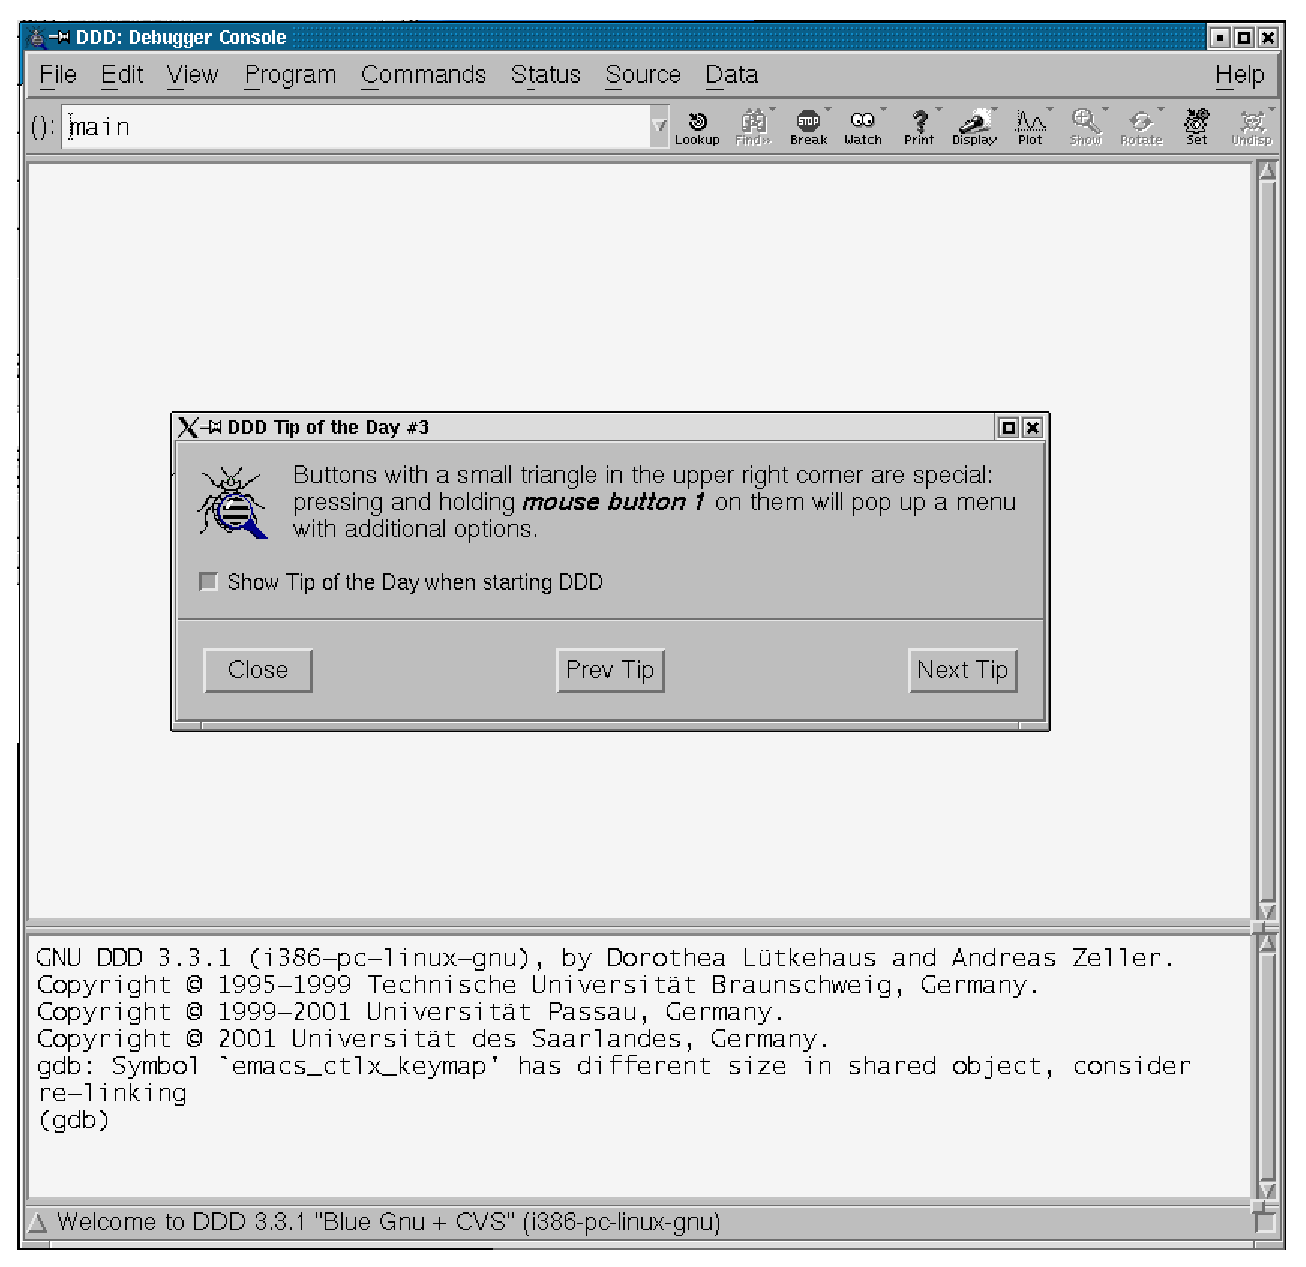
\includegraphics[width=\textwidth]{imagenes/ddd_inicio.eps}
\caption{Pantalla de inicio}
\end{figure}

Este es  el aspecto que  presenta el  {\tt ddd} cuando  lo arrancamos,
vamos a ir por pasos mostrando  lo que normalmente un programador como
nosotros vamos a necesitar de un depurador.

\subsection{Mostrar el contenido de las variables}

Para mostrar el contenido de las  variables lo que tendremos que hacer
es, como se dice coloquialmente, colocar un {\em watch} a la variable.
En {\tt ddd} esto  es muy sencillo de hacer y  hay varias maneras, una
de ellas puede ser  escribir el nombre de la variable  en el cuadro de
texto que  tenemos justo por  debajo de la barra  de men� y  pulsar el
bot�n de watch que est� al mismo nivel un poco m�s a la derecha:

\begin{figure}[hbtp]
\centering
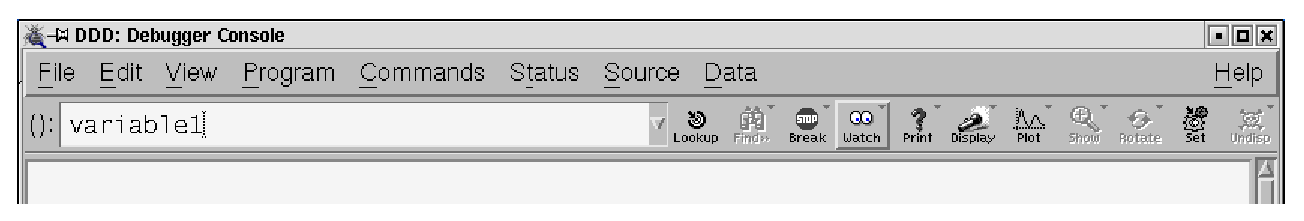
\includegraphics[width=\textwidth]{imagenes/ddd_watch.eps}
\caption{Barra de herramientas}
\end{figure}

Otra forma de hacerlo quiz� m�s r�pida poner el cursor del rat�n sobre
el nombre de la variable en  el c�digo fuente, pulsar el boton derecho
y escoger la opcion display.

\begin{figure}[hbtp]
\centering
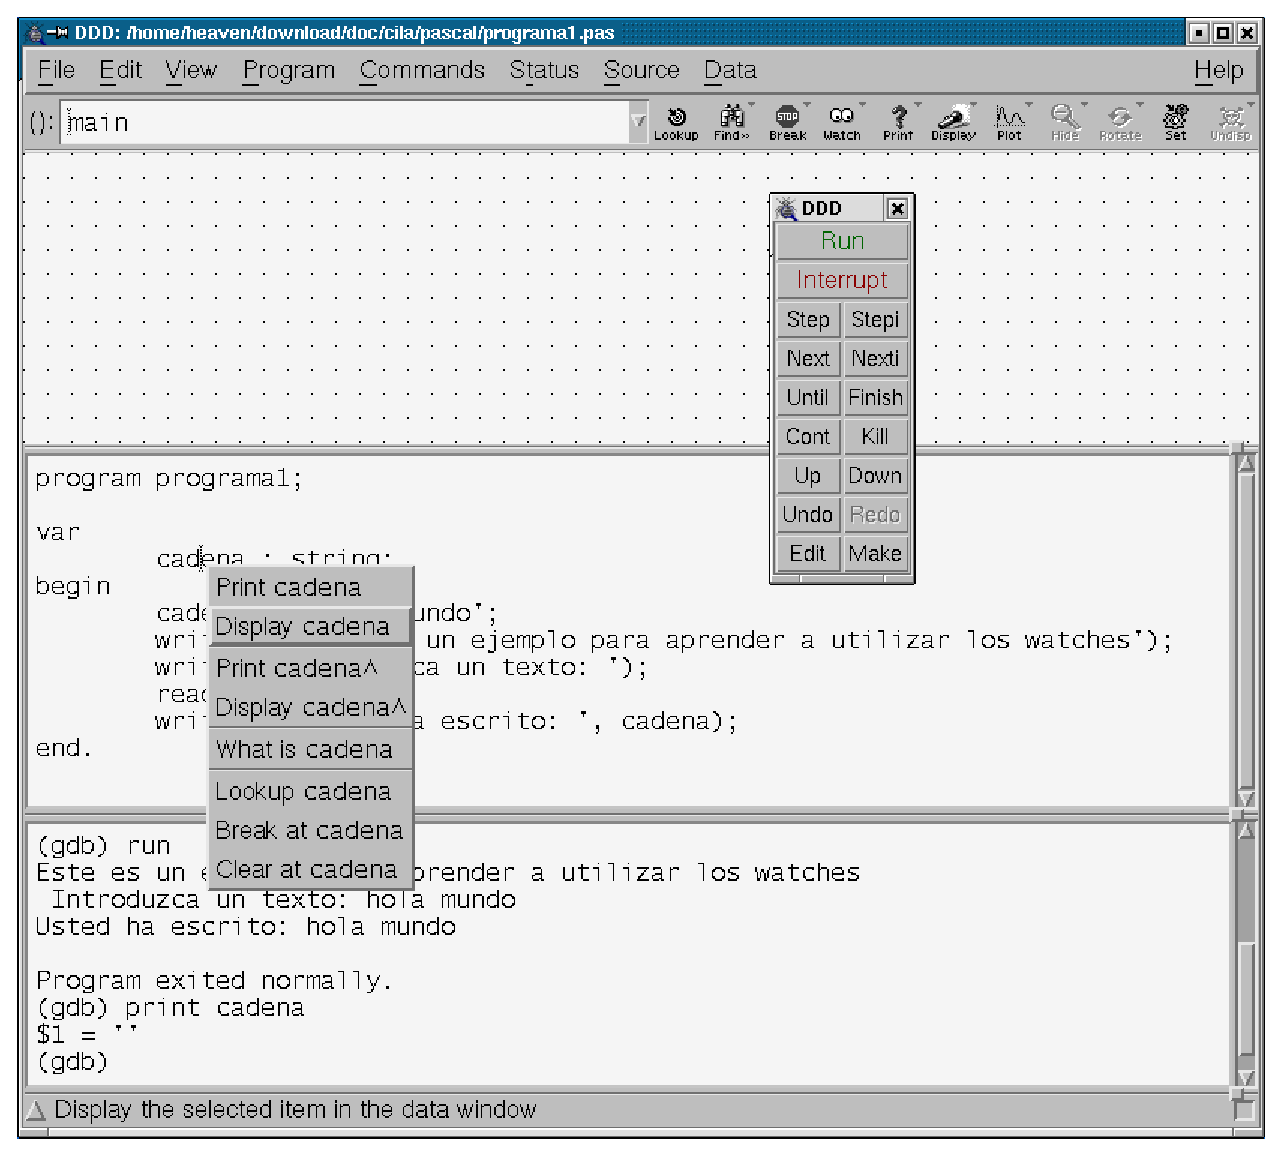
\includegraphics[width=\textwidth]{imagenes/ddd_watchII.eps}
\caption{Watches}
\end{figure}

\subsection{Colocar puntos de  ruptura}

Bueno, ya tenemos un watch de la variable, pero\ldots �que pasa cuando
pulsamos sobre  el bot�n  de run?  �No vemos nada!  bueno, eso  es una
circunstancia pasajera, vamos  a colocar un {\em  breakpoint} o punto
de ruptura.

Los  breakpoints son  lugares  donde el  depurador  har� que  nuestro
programa   pare  la   ejecucu�n   para,  de   esta  manera,   analizar
detenidamente el estado  de nuestro programa. La manera  de colocar un
breakpoint en el  {\tt ddd} es simplemente desplazarse hasta  la l�nea donde
deseamos colocar  el breakpoint y  hacer un  doble click con  el boton
izquierdo del rat�n.

Vemos que se nos coloca un s�mbolo  de stop donde hemos hecho el doble
click,  lo que  indica que  hay un  breakpoint. Si  pulsamos sobre  el
breakpoint  con el  boton derecho  vemos que  se nos  da la  opcion de
desactivarlo, quitarlo y una muy  extra�a de propiedades. La opcion de
propiedades hace  que nos  aparezca un  cuadro de  dialogo en  el cual
podemos introducir una expresi�n, �sta expresi�n se utiliza para hacer
que nuestro breakpoint sea inteligente  y no pare la ejecuci�n siempre
que  el programa  pase por  all�, sino  que solo  se parar�  cuando la
expresi�n  se cumpla,  por ejemplo,  si ponemos  el breakpoint  en un
bucle con 10.000 iteraciones y nosotros queremos que se pare cuando la
i (variable  que cuenta  las iteraciones)  llegue a  5000 pues  lo que
hemos de poner en  propiedades del breakpoint es {\tt i  = 5000} y de
esa manera  nos saltaremos  las 5000 primeras  iteraciones que  no nos
interesan.

\begin{figure}[hbtp]
\centering
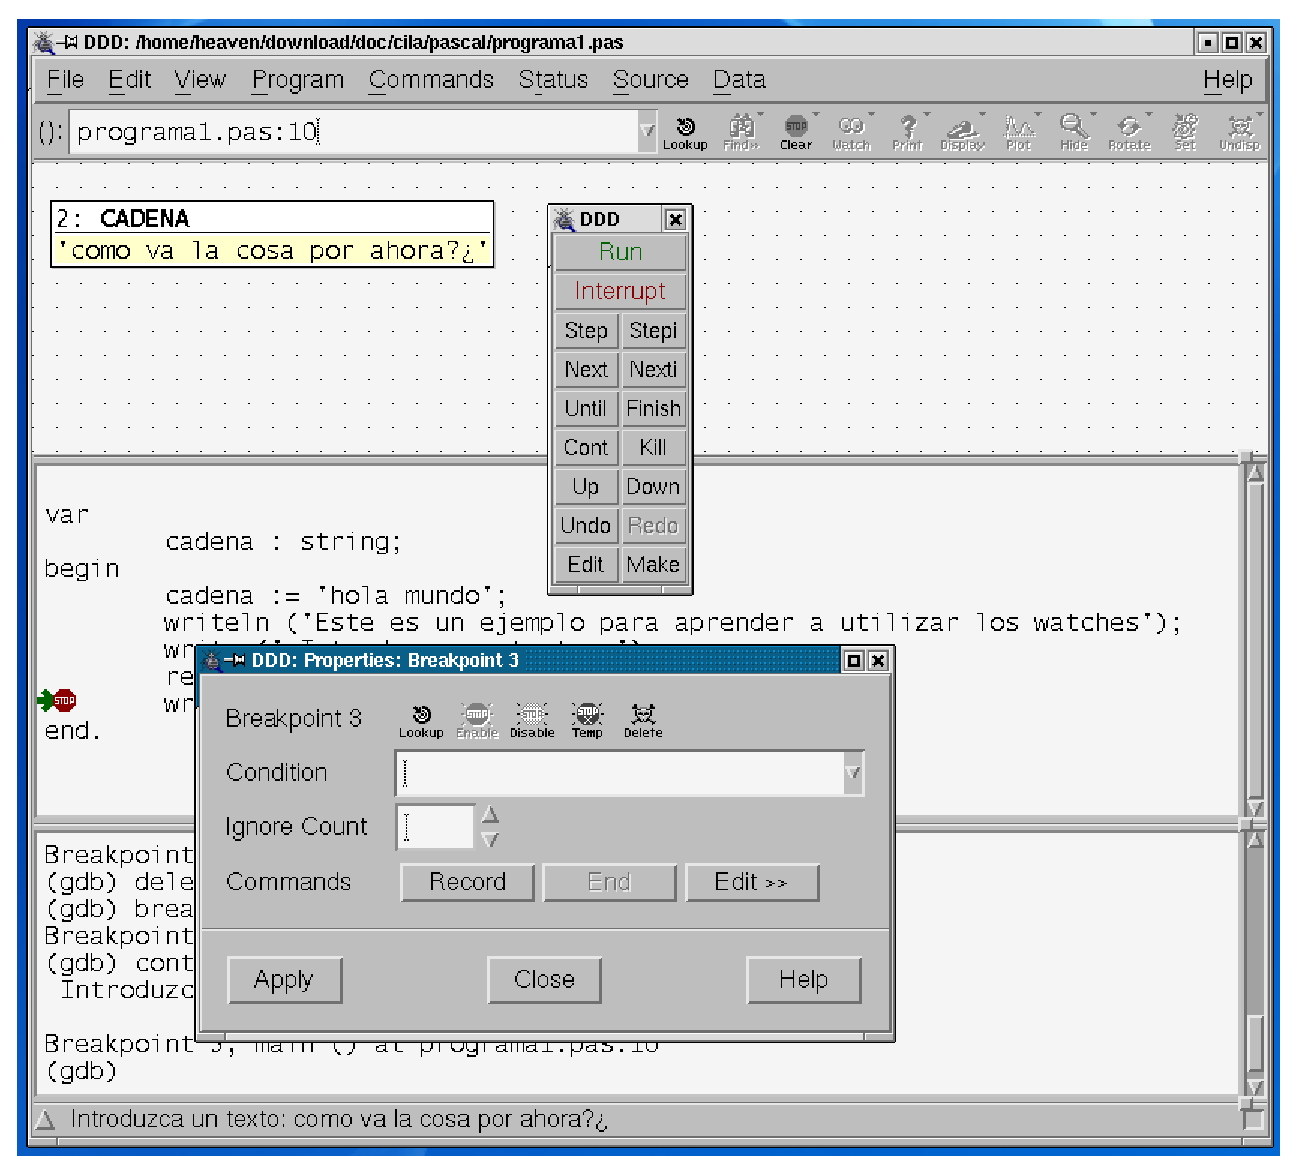
\includegraphics[width=\textwidth]{imagenes/ddd_breakpoint.eps}
\caption{Breakpoints, o puntos de ruptura}
\end{figure}

\subsection{Ejecuci�n paso a paso}

Ahora que  ya tienes un  watch y un  breakpoint, en este  momento solo
podemos ir  saltanto de  breakpoint en  breakpoint, y  esto no  nos es
suficiente  as�  que  vamos  a  intentar controlar  m�s  el  flujo  de
ejecuci�n  de  nuestros  programas.  Para esta  tarea  tenemos  varias
herramientas comunes en  la mayor�a de depuradores, en el  caso del dd
las encontramos en una ventana que tenemos flotando sobre el depurador,
con lo cual no es complicado utilizarlas, siempre las tenemos a mano y
son las siguientes:

\begin{description}

\item[{\em Step}:]{(paso) esta herramienta nos  sirve, como su propio nombre
indica, para  ejecutar nuestro  programa paso  a paso.  Normalmente lo
que  hacemos es  colocar  un  breakpoint al  inicio  de  la funcion  o
procedimiento que  queremos analizar  y luego  ir pulsando  {\tt step}
para analizar sentencia a sentencia que es lo que hace nuesto c�digo.}

\item[{\em Next}:]{(siguiente) muy  parecida a step, solo  que pulsando {\tt
next} si en el c�digo hay una llamada a una funcion o procedimiento no
entramos  en  ella, sino  que  ejecuta  �sta  y  nos colocamos  en  la
siguiente l�nea del programa.}

\item[{\em Until}:]{(hasta)  esta herramienta  nos  sirve  para ejecutar  el
programa hasta  la posici�n actual  del cursor,  es muy parecida  a un
breakpoint temporal.}

\item[{\em Cont}:]{(continuar)  saltamos  hasta  el siguiente  breakpoint  o
hasta el final del programa si es  que no hay ning�n breakpoint m�s en
el flujo de ejecuci�n.}

\end{description}

A  parte de  estas  herramientas  tenemos algunas  m�s  que se  suelen
utilizar  menos, por  ejemplo  aquellas que  ejecutan exactamente  una
instrucci�n (de c�digo m�quina).

\subsection{Visi�n de punteros}

Probablemente estabas deseando que existiera  una cosa como la que vas
a ver. No te asombres de la  potencia de este depurador, es uno de los
pocos que lo  hacen y de ah�  viene su buena fama. La  capacidad de la
que hablamos es la de {\em ver} los punteros.

Seguramente has hecho  m�s de un programa con memoria  din�mica que no
acababa de  funcionar bien porque se  te perd�an punteros y  no sabias
muy bien  por donde andaban  o a  d�nde estaban apuntando,  pues bien,
esto ya no es excusa para entregar  una pr�ctica a medio hacer, el {\tt ddd}
viene en nuestra ayuda y  tenemos la {\sf herramienta definitiva} para
la depuraci�n con punteros.\\

Cuando  haces un  watch de  una  estructura (record)  salen todos  los
campos en un  recuadro y los punteros tambi�n salen  como otro tipo de
dato  cualquiera. Cuando  tienes {\tt  \$0}  en la  informaci�n de  un
puntero quiere  decir que  el puntero  es {\tt  Nil} (nulo),  y cuando
tenemos un n�mero  precedido del s�mbolo {\tt \$} quiere  decir que el
puntero est� apuntando  a esa zona de memoria, por  lo tanto, podremos
mostrar el  contenido de esa  zona de memoria. Si  decidimos mostrarla
aparecer�  otro cuadro,  como  el que  inicialmente  ten�amos, con  la
informaci�n de  la zona de memoria  apuntada por el puntero  que hemos
decidido expandir  y una  flecha desde el  recuadro original  hasta el
nuevo, marcada con el nombre del puntero expandido.

De  esta manera  es  muy sencillo  seguir  los punteros  y  ver a  que
posiciones est�n apuntando, ver si  estamos asignando cosas a punteros
que son nulos as� como que pinta va teniendo la estructura que estamos
construyendo en memoria, lo cual ayuda  mucho a la hora de moverse por
las estructuras que fabricamos.

Un ejemplo  de lo  que se puede  hacer es mostrar  un �rbol  para, por
ejemplo, comprobar que todos los  punteros que salen de nuestros nodos
hoja est�n  a {\tt  Nil} y  de esa manera  asegurarnos de  que nuestro
programa no va a fracasar.


\begin{figure}[hbtp]
\centering
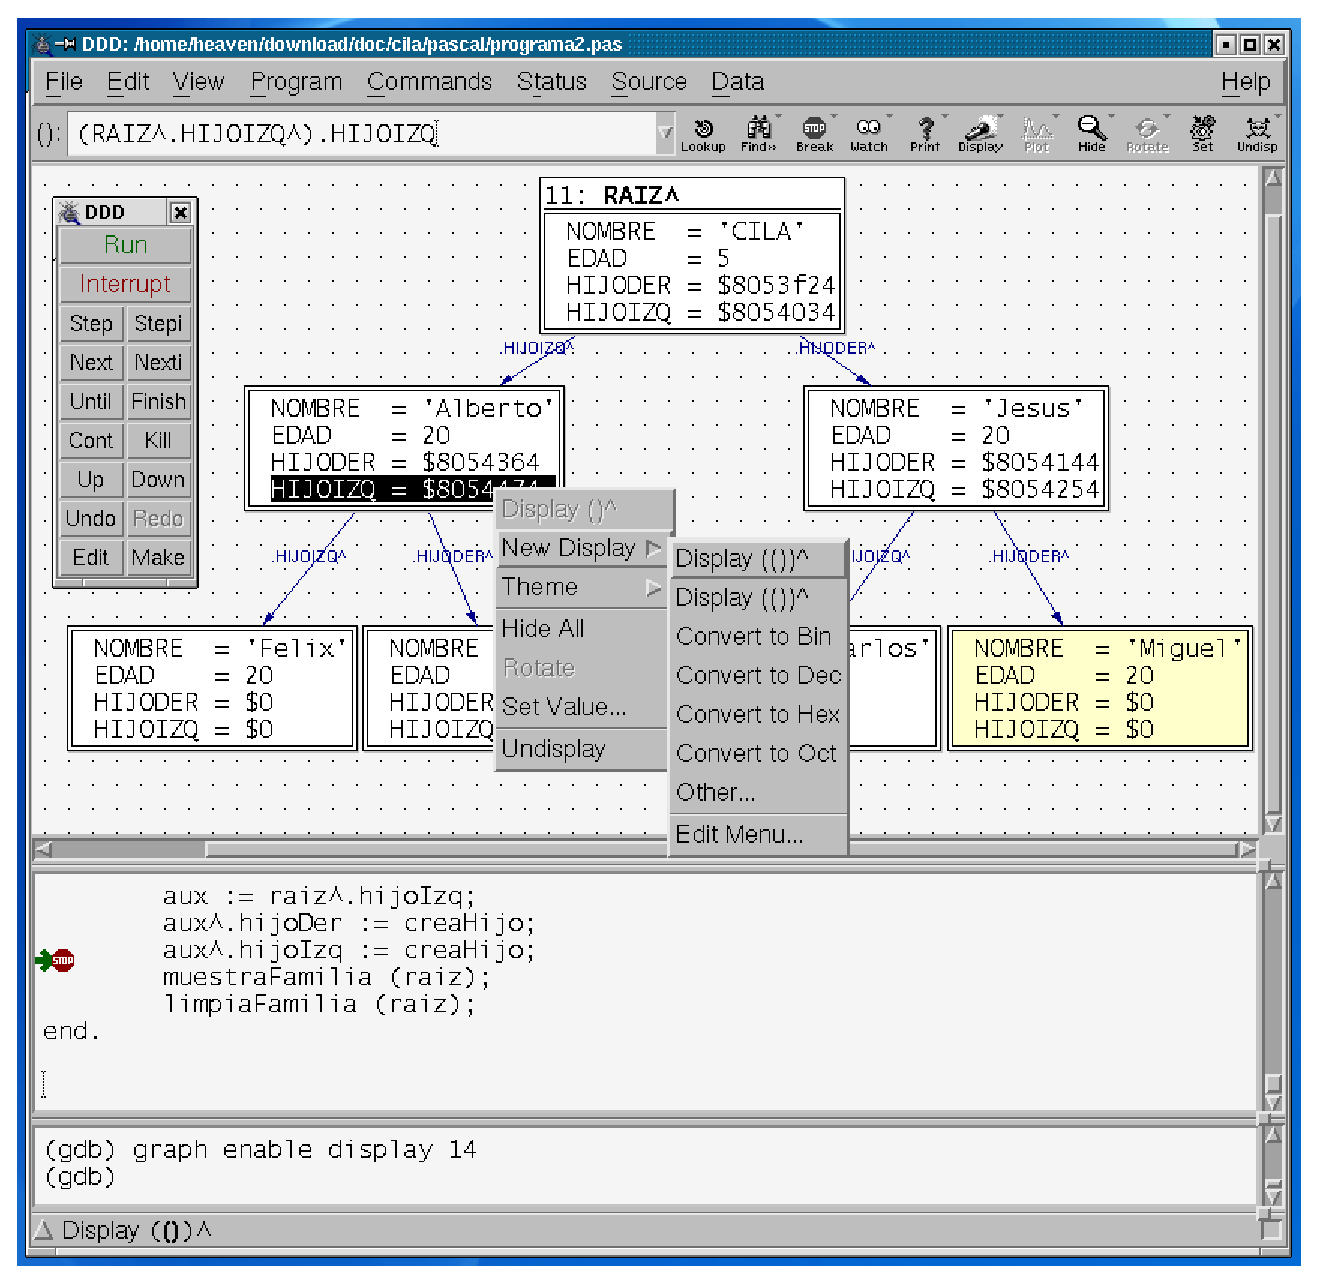
\includegraphics[width=\textwidth]{imagenes/ddd_punteros.eps}
\caption{Estructura de un �rbol binario}
\end{figure}

%Autor: Carlos de la Cruz (frodo@fmat.ull.es)

\chapter{Java}


Java es un lenguaje de alto nivel y de prop�sito general. Al principio
fue desarrollado  en los laboratorios  de {\em Sun  Microsystems} para
servir en aparatos de electr�nica de consumo, como videotel�fonos, set
boxes (descodificadores), o aparatos similares, pues pretend�a hacerse
un lenguaje  lo m�s independiente posible  de la plataforma en  la que
fueran a ser ejecutados los programas hechos con �l.

A  diferencia  de otros  muchos  lenguajes  compilados, el  compilador
de  java no  genera  ficheros ejecutables.  Genera  unos ficheros  con
extensi�n  {\tt  .class}  llamados  {\em  bytecodes}.  Estos  ficheros
posteriormente podr�n ser ejecutados  mediante la {\em M�quina Virtual
Java} (JVM en  ingl�s), que es la encargada de  ejecutar los programas
de java.

Esto, que a primera vista puede  parecer tedioso e in�til, es una gran
ventaja para la portabilidad del c�digo, pues cada plataforma tiene su
propia M�quina Virtual Java: Apple Mac OS tiene una, Linux tiene otra,
Windows otra, Amiga OS tambi�n, etc. Esto implica que si desarrollamos
un  programa en  un iMac  con  Linux, el  amigo que  tenga un  potente
servidor SUN podr� ejecutar nuestra aplicaci�n hecha en Java, al igual
que nosotros  podremos utilizar el  complicado programa de  c�lculo de
estructuras que otra  persona ha desarrollado en su Pc  con Windows en
el trabajo.

Realmente, Java no es tan bonito  como lo estamos pintando. Uno de sus
principales  puntos  d�biles es  que  no  es  demasiado r�pido,  y  es
bastante  caprichoso en  cuestiones de  recursos de  hardware. Adem�s,
existen  dos m�quinas  virtuales Java,  la de  Microsoft y  la de  SUN
Microsystems, que presentan algunas incompatibilidades.

Pero su principal  ventaja es la impresionante  portabilidad, as� como
su utilidad en campos como Internet (donde principalmente se usa en la
actualidad), en servidores web.

Los  programas   java  podemos   clasificarlos  b�sicamente   en  tres
categor�as: {\em  applets}, {\em  servlets} y aplicaciones  {\em stand
alone}.

\begin{itemize}

\item  Los {\em  applets}  son peque�as  aplicaciones  creadas con  el
prop�sito de ser incluidas en p�ginas web. Cuando el cliente, desde su
navegador web con  java incorporado pide esa p�gina web,  el applet se
descarga  a su  ordenador donde  comienza su  ejecuci�n. El  navegador
tiene la maquina virtual java incorporada.  Los applets son el tipo de
aplicaciones  java que  m�s restricciones  de seguridad  presentan. No
pueden acceder  al sistema de  archivos local fuera del  directorio en
que se  ejecutan, no pueden  abrir ventanas adicionales sin  que �stas
aparezcan se�alizadas  con el indicativo: ``Warning:  applet window'',
ni  hacer muchas  cosas  que podr�an  ser  perjudiciales para  nuestro
ordenador.

\item  Las  aplicaciones  que  a   nivel  de  seguridad  permiten  m�s
libertades que los applets.

\item Los  {\em servlets} son una  especie de applets que  se ejecutan
s�lo en  el servidor  web cuando  uno pide una  p�gina, y  que generan
din�micamente  p�ginas  a  partir  de fuentes  como  bases  de  datos,
terceros programas que recopilan informaci�n, etc�tera.

\end{itemize}

 A nivel visual,  java tiene dos grupos de controles,  widgets, o como
prefiramos  llamarlos (no  son  otra  cosa que  los  campos de  texto,
formularios, botones, etc.):

\begin{itemize}

\item El  Java AWT,  (Advanced Window  Toolkit), obsoleto  y mantenido
s�lo por compatibilidad en versiones actuales de java.

\item  El conjunto  de widgets  {\bf  Java Swing},  que presenta  unos
controles mucho m�s est�ticos y es mucho m�s flexible.

\end{itemize}

Ambos  conjuntos de  widgets  proporcionan  una presentaci�n  uniforme
independiente de la plataforma en que sean ejecutados. Adem�s, otro de
los principales atractivos de java es  que el compilador no nos cuesta
nada.  Se  encuentra  disponible  para bajarlo  de  java.sun.com  para
cualquiera de las plataformas m�s comunes en el mercado.

Veamos c�mo se generan programas  b�sicos en java mediante un ejemplo.
En un  editor escribimos  el siguiente  c�digo y  lo guardamos  con el
nombre de fichero {\tt Prueba.java}.


\begin{verbatim}
// Ejemplo 1 de Java para CILA
// Fichero: HolaMundo.java

public class HolaMundo {
       public static void main(String[] argv){
	      System.out.println("Hola mundo");
}
}
\end{verbatim}

Es de vital importancia que el  nombre del fichero coincida con lo que
escribimos despu�s  de ``{\tt public  class}''. Asimismo, Java  es un
lenguaje muy exigente  en materia de may�sculas y  min�sculas, como de
de espacios y  tabuladores. Para compilar este  programa utilizamos el
siguiente comando:

\begin{verbatim}
$ ls
HolaMundo.java

$ javac HolaMundo.java

$ ls
HolaMundo.java  HolaMundo.class

\end{verbatim}


Obtendremos  un fichero  con extensi�n  {\tt  .class} que  es el  {\em
bytecode}, el fichero que ejecutaremos con el siguiente comando:


\begin{verbatim}
$ java HolaMundo
Hola Mundo
\end{verbatim}

Lo que no tiene sentido es poner ``{\tt  java  Prueba.class}'', pues no
funcionar�a, devolviendo el siguiente error:

\begin{verbatim}
$ java HolaMundo.class
Can't find class HolaMundo.class
\end{verbatim}

\begin{verbatim}
$ java HolaMunco.class
Exception in thread "main" java.lang.NoClassDefFoundError: HolaMundo/java
\end{verbatim}

Veamos ahora un ejemplo de {\em applet}. Tecleamos el siguiente c�digo
y lo guardamos como {\tt HolaMundo2.java}.

\begin{verbatim}
// Ejemplo 2 de Java para CILA
// Fichero: HolaMundo2.java

import java.applet.Applet;
import java.awt.*;

public class HolaMundo2 extends Applet {
    public Button botonUno = new Button ("Hola Mundo");
    public void init() {
    add ( botonUno );
    }
}
\end{verbatim}

Compilamos  el  applet del  mismo  modo  que  hicimos con  el  ejemplo
anterior:

\begin{verbatim}
$ javac HolaMundo.java
\end{verbatim}

Con esto generamos  el fichero {\tt HolaMundo2.class}  que contiene el
applet. Ahora necesitamos una p�gina  web que cargue el applet. Creamos
el fichero {\tt HolaMundo2.html} con el siguiente c�digo:

\begin{verbatim}
<html>
<head>
<title> Ejemplo 2 de Java para CILA </title>
</head>
<body>
<center>
<applet code="HolaMundo2.class" width="300" height="300" ></applet>
</center>
</body>
</html>
\end{verbatim}

Para probar el applet utilizaremos  el m�todo que utilizar�a cualquier
visitante, cargarlo desde la p�gina web que hemos creado a tal efecto.
Esto lo hacemos  con cualquier navegador que soporte,  Java, entre los
que recomendamos Netscape.

\begin{verbatim}
$ netscape HolaMundo2.html
\end{verbatim}

Veremos como el applet se ejecuta  dentro de la p�gina web. Otra forma
de ejecutar un applet de  Java, por ejemplo cuando estamos programando
y s�lo  deseamos probarlo  pero no queremos  ejecutar netscape,  es el
programa appletviewer que proporciona el JDK.

\begin{verbatim}
$ appletviewer HolaMundo2.html
\end{verbatim}

Podemos apreciar la  diferencia entre un {\em  applet}, cuya ejecuci�n
est� controlada por el navegador y se  limita a la p�gina web desde el
que  es  cargado,  y  una  aplicaci�n  intependiente  que  se  ejecuta
directamente en  la consola del  sistema sin m�s intermediario  que la
M�quina Virual Java.




% M�dulo VI:  Programaci�n avanzada
% 1. PHP + [My|Postgre]SQL
% 2. Perl
% 3. Python (NumPy) 
% 4. GUIs toolkits: Tk, QT, Wx, Gtk, Glade
% 5. XML
\part{Programaci�n avanzada}
%Autor: Carlos de la Cruz (frodo@fmat.ull.es)

\chapter{PHP}

\section{Introducci�n}

PHP es  un lenguaje dise�ado  para la generaci�n din�mica  de p�ginas.
web Los  ficheros de PHP  se almacenan en  el servidor y  se ejecutan.
cuando un  usuario introduce en su  navegador la direccion de  una de.
estas p�ginas. Estas, a su vez, contienen c�digo a partir del cual se.
generan p�ginas est�ticas en formato HTML                            .

La utilidad de  esto es que podemos crear  autom�ticamente p�ginas web
que se actualicen solas, bas�ndose en una fuente de datos.

Por  ejemplo, si  quisi�ramos que  cada vez  que el  usuario accede  a
nuestra p�gina, en esta apareciera la fecha y la hora, ser�a imposible
conseguirlo a partir de ficheros est�ticos ``html''.

Por  tanto,  la  soluci�n  ser�a  tener  en  el  servidor  un  fichero
``hora.php'',   mediante  el   cual,  cuando   alguien  accediera   a:
http://miservidor.com/hora.php, tuviera la hora del instante en que se
ejecut� el c�digo php.

Cada vez que alguien le diera a ``recargar'' en el navegador, ver�a la
hora actual.

Pero como podremos comprobar,si se hace  clic en el bot�n ``ver c�digo
fuente'' del navegador, s�lo veremos, por ejemplo ``12:02:12''.

PHP tiene  todas las  ventajas que  tienen otros  lenguajes utilizados
para generaci�n din�mica de contenido web como PERL y ASP, y otras que
ninguno de estos  permiten hacer de una forma flexible  y c�moda, como
por  ejemplo la  generaci�n  din�mica de  pel�culas Macromedia  Flash,
im�genes (con el m�dulo GDLib), informes en formato PDF, etc.

\section{Primeros Pasos}

Todo script php est� delimitado por los identificadores \verb+<?php+ y
\verb+?>+. Dentro de estos s�mbolos, va  escrito todo el c�digo php de
este.

La primera funci�n que veremos de PHP ser� ''echo'', que nos permite imprimir
texto o tags HTML en nuestra p�gina. La funci�n echo va siempre acompa�ada de
unos par�ntesis y comillas(simples o dobles) en caso de que vayamos a imprimir una o varias cadenas est�ticas de texto, y puede ir o no acompa�ada de estos en caso de que vayamos a imprimir s�lo el contenido de una o varias variables.


Como con el resto de los lenguajes, vamos a empezar viendo como ser�a un "hola mundo" en PHP.

\begin{verbatim}
<?php

echo("<center><font size=7>Hola, Mundo!</font></center>");

?>
\end{verbatim}

Este sencillo  script nos permite  ver como diferenciar el  c�digo PHP
del c�digo HTML,  pues si introduj�ramos c�digo HTML  suelto dentro de
los delimitadores \verb+<?php+  y \verb+?>+, el m�dulo  PHP de nuestro
servidor web provocar�a un error de interpretaci�n.

PHP es un lenguaje muy flexible. Nos permite imprimir el valor de variables
dentro de cadenas de texto sin tener que cerrar y volver a abrir comillas, de
la siguiente forma:
\begin{verbatim}
<?php

$limones=2;
$naranjas=3;

echo("Tenemos $limones limones y $naranjas naranjas.");
?>

\end{verbatim}

F�jate que no es lo mismo escribir:
{\tt echo("Tenemos $limones limones y $naranjas naranjas."); } que
{\tt echo('Tenemos $limones limones y $naranjas naranjas."); }.

La primera l�nea, para $limones=2 y $naranjas=3 imprimir� "Tenemos 2 limones y 3 naranjas", mientras que la segunda imprimir� ''Tenemos $limones limones y $naranjas naranjas". Es decir, si utilizamos las dobles comillas, tendremos que los valores de las variable se despliegan dentro de estas. Si utilizamos, por el contrario, comillas simples, lo que haya entre ellas se imprimir� tal cual.

Es importante saber que cuando uno necesita utilizar comillas en el HTML resultante de nuestro script PHP, conviene que ''escape'' las comillas, o de lo contrario el interpretador mostrar� una p�gina con un error de compilaci�n.

por ejemplo, si queremos mostrar el tag html:

{\tt <a href="http://www.fmat.ull.es/~frodo">}, tendremos que hacerlo de la siguiente forma en php:
{\tt echo("<a href=\"http://www.fmat.ull.es/~frodo\">");}. (F�jate en las barras invertidas que se anteponen a cada una de las comillas que van dentro del par de comillas de la funci�n "echo".

Para la inclusi�n de c�digo HTML previamente escrito dentro de una p�gina que se genera din�micamente (por ejemplo, sup�n que tienes una cabecera, un pie de p�gina predefinidos para tu sitio web, y quieres que var�e s�lo el cuerpo de la p�gina, para darle un dise�o uniforme), utilizamos el comando {\tt include}.

Por ejemplo:

\begin{verbatim}
<?php

include "include/cabecera.php";
echo("Hola! este es el cuerpo de la p�gina");
include"include/pie.php;

?>

\end{verbatim}





\section{Estructuras de datos}

B�sicamente, existen los escalares, los hash y los arrays.


\section{Estructuras de control}

Para el uso de las estructuras de control PHP es muy parecido al lenguaje ''C'', tanto por el uso de llaves para delimitar los bloques de c�digo como por usar la misma sintaxis. Distinguiremos dos tipos de estructuras de control:

\subsection{Condicionales: If, Switch}

If: Este condicional nos permite ejecutar un bloque de c�digo en caso de que se
de una condici�n determinada. Veamos un ejemplo:

\begin{verbatim}
<?php

$a = 2;
$b = 10;

if ($a<$b) {
	echo("Hey!, parece que \$a vale $a, que es mayor que \$b, que vale $b");
	}
	
?>

Como, evidentemente 2 siempre ser� menor que 10, el bloque de c�digo entre llaves se ejecutar�a siempre.

\end{verbatim}

\subsection{Repetitivas: While,For}

\section{Como estructurar nuestro c�digo en php}

Las funciones. function chona($lalala,$otroparametro)

\section{Manejo de formularios}


\section{Utilizaci�n de bases de datos}
Aunque PHP soporta varias clases de servidores de base de datos, debido a que cada uno usa un interfaz distinto, resulta bastante inc�modo tener que aprender las funciones de PHP para cada uno de ellos. Es por ello que suelen utilizarse librer�as adicionales (no incluidas con PHP, pero s� con la mayor�a de las distribuciones Linux), como la que utilizaremos en este texto/curso: AdoDB.

AdoDB nos permite cambiar de sistema de bases de datos simplemente cambiando un par�metro al realizar la conexi�n a la Base de datos (BDD de ahora en adelante) , de forma que una aplicaci�n PHP dise�ada para correr con Oracle, puede ser portada para funcionar en MySql, Informix, etc. con tan s�lo cambiar una l�nea de c�digo.


\section{Creaci�n de im�genes din�micamente}

\section {Bibliograf�a recomendada}



%Autor: MojoPiKon

\chapter{Perl}

\section{Que es PERL}

PERL es un lenguaje de scripts o guiones creado por Larry Wall en 1988, que, a pesar de haber tenido su m�xima difusi�n con la aparici�n de internet y el web, viene siendo utilizado desde hace varios a�os por administradores de sistemas para la automatizaci�n de tareas rutinarias, como pueden ser gesti�n de grandes vol�menes de usuarios, b�squeda de patrones de texto mediante expresiones regulares, realizaci�n de copias selectivas de seguridad, etc.

% Existen una enorme variedad de m�dulos para PERL (baste decir el listado de ellos en texto plano ocupa varios megabytes). Tanto este listado como estos m�dulos pueden encontrarse en la web de recursos para perl http://www.cpan.org

Como lenguaje interpretado, su potencia radica en su gran portabilidad siempre que los m�dulos que se empleen se encuentren en la plataforma en que el script vaya a ser utilizado.

Pese a la creencia popular, PERL sirve para desarrollar casi cualquier tipo de programa, pues entre sus m�dulos se encuentran, por poner algunos ejemplos, m�dulos de OpenGL (Especificaci�n para la creaci�n de gr�ficos 3D),para el tratamiento de audio digital, o para la creaci�n de interfaces gr�ficas, ya sea bajo plataformas corriendo sistemas GNU/Linux,Variantes de UNIX,Apple MacOs, Microsoft Windows, etc.

\section{Donde conseguir PERL}

La versi�n oficial de PERL est� disponible de forma gratuita en la web oficial del proyecto PERL (http://www.perl.org) para las distintas plataformas anteriormente citadas.

Por otro lado, hay distribuciones empaquetadas por empresas, con algunos m�dulos m�s que la versi�n oficial ``base''.

Destaca por su comodidad de instalaci�n y la cantidad de m�dulos disponibles ``activeperl'', de activestate (http://www.activestate.com).

Activeperl est� disponible para Linux y para Windows, y puede ser descargado tambi�n de forma gratuita.

\section{Primeros pasos}

PERL lee los scripts a partir de ficheros de texto plano. Para ejecutarlos, suele procederse de la siguiente manera:

\begin{verbatim}

14:16:14 wd:~ u:frodo> perl fichero.pl

\end{verbatim}

Esto ejecuta el gui�n contenido en el fichero ``fichero.pl''. Esto no resulta muy sorprendente, desde luego.

Para ejecutar scripts PERL en GNU/Linux o UNIX, podemos recurrir a colocar al principio del gui�n una l�nea como esta:

\begin{verbatim}

#!/usr/bin/perl

\end{verbatim}

Con esto conseguiremos, tras dar permisos de ejecuci�n al script mediante chmod 755 fichero.pl, poder ejecutarlo poniendo desde el shell:

\begin {verbatim}

./programa.pl

\end{verbatim}

Para probar que realmente nuestro int�rprete PERL funciona correctamente, probemos un apasionante y a la vez complejo programa:

\begin {verbatim}

#!/usr/bin/perl / 
print ``Hola mundo!\n'';

\end{verbatim}

\section{Entrada,salida y sint�xis b�sica}

La sint�xis de PERL a muchos programadores nos recuerda a la de C, por que emplea llaves ``{ }'', puntos y comas al final de las l�neas, e incluso gran parte
de las estructuras de control de C, las cuales se manejan de forma casi id�ntica en ambos lenguajes, y que veremos en el siguiente apartado. 

Para insertar comentarios en nuestro c�digo, emplearemos el caracter de ``almohadilla''.

\begin{verbatim}
# Esto es un comentario en PERL. Esta l�nea no hace nada, pero tampoco
# provoca errores de compilaci�n en nuestro programa.
\end{verbatim}

Las variables en PERL son de tres tipos: arrays, escalares y estructuras ``hash''. Estas ser�n descritas en profundidad en la secci�n ``Estructuras de datos, de control y operadores''. De momento, nos contentaremos con saber que los escalares son variables que s�lo almacenan UN dato y que pueden contener datos num�ricos, cadenas ascii, etc y que se denotan anteponiendo a su nombre un signo de dolar. Se aplican las normas estandar de otros lenguajes para nombrar estas variables, como son no utilizar n�meros al principio del identificador, no utilizar espacios y no utilizar palabras reservadas como identificadores.
Cualquier omisi�n en el cumplimiento de estas normas provocar� irremisiblemente un error de interpretaci�n.


Se puede hacer corresponder a una variable de tipo escalar una cadena mediante el uso de el igual y las comillas simples. Para los valores num�ricos se pone s�mplemente el igual y el valor, sin comillas. Ejemplo:

\begin{verbatim}

$nombre = 'Fernando';
$edad = 19;
$numero_de_piso = '5';


\end{verbatim}

N�tese que si pusieramos las comillas para asignar un valor num�rico a una variable escalar, PERL interpretar�a dicha variable como una cadena de caracteres ASCII, por lo que no podr�amos, por ejemplo, sumar o restar dichos n�meros.

Es importante conocer que podemos utilizar tanto comillas simples como comillas dobles para asignar cadenas a escalares. Pero existe una diferencia.

\begin{verbatim}
$nombre = ``Carlos'';

print''Me llamo $nombre\n''; # Imprime: Me llamo Carlos
print 'Me llamo $nombre''; # Imprime: Me llamo $nombre\n

\end{verbatim}


Ahora que ya sabemos lo b�sico de las reglas del juego, veamos algo m�s sobre la funci�n print.





\section{Estructuras de control, de datos y operadores}





\section{Manejo de Cadenas}

\section{Ficheros}

\section{Automatizaci�n de tareas y ejecuci�n de comandos externos}

\section{Interfaces b�sicas de usuario en modo texto}

\section{Bibliograf�a recomendada}


%Autor: miguev

\chapter{Python}



\chapter{GUIs y toolkits}


\chapter{XML}



% Ap�ndices y referencias
\appendix
%Autor: todos
  
\chapter{Recursos en internet}
\label{recursos}  

La mayoría  de los recursos que  podamos necesitar para usar  Linux se
encuentran  distribuidos por  Internet,  y una  enorme cantidad  están
disponibles en español.

\begin{itemize}

\item {\tt http://www.debian.org} -- El Proyecto Debian es una asociación
  de  personas  que  han  hecho  causa común  para  crear  un  sistema
  operativo (SO)  libre. Este  sistema operativo  que hemos  creado se
  llama Debian GNU/Linux, o simplemente Debian para acortar.

\item {\tt http://www.redhat.es} --  La  primera  distribución Linux  en
  reorientarse hacia los usuarios finales.

\item {\tt http://www.linux-mandrake.com/es/} -- Linux-Mandrake es
  un amigable  Sistema Ope\-ra\-ti\-vo  Linux. Es  muy fácil  de usar,
  tanto en el  hogar u oficina como en servidores.  Está disponible en
  forma gratuita en varios idiomas alrededor del mundo.

\item {\tt http://www.ututo.org} -- Un GNU/Linux Simple.

\item {\tt http://www.linux-es.com} -- Existen muchos lugares en
  Internet  dedicados  a  LINUX,  pero  la mayoría de ellos están en
  inglés. Estas páginas  pretenden  ser un  punto  de  partida  para
  aquellos  que necesitan encontrar información sobre este sistema y
  en  la  medida de lo posible se ha intentado que la mayoría de los
  enlaces y contenidos sean en castellano.

\item {\tt http://www.gnu.org/home.es.html} -- El  Projecto  GNU
  comenzó en  1984 para  desarrollar un sistema  operativo tipo Unix
  completo, el cual  es  software libre:  El  sistema  GNU. Variantes
  del  sistema GNU, utilizando Linux  como  kernel,  son  ampliamente
  usadas, y aunque frecuentemente llamadas ``Linux'', dichas variantes
  deberían referirse más exactamente como sistemas GNU/Linux.

\item {\tt http://es.tldp.org}  --  Proyecto LuCAS  -  La
  mayor biblioteca en español dedicada a GNU/LiNUX de todo el planeta

\item {\tt http://www.insflug.org}  --  En  el INSFLUG  se  coordina
  la traducción ``oficial'' de documentos  breves, como los COMOs  y
  PUFs o  Preguntas de Uso Frecuente, las FAQs  en inglés. Esperamos
  que la información que encuentre aquí le sea de utilidad.

\item {\tt http://www.gnu.org/software/emacs/emacs.html} --  Es un
  editor de  pantalla y  ambiente  para cómputo  de  tiempo real,
  extensible  y  personalizable.  Ofrece Lisp (finalmente integrado al
  editor)  para escribir  extensiones  y proporciona  una interfaz  al
  sistema de ventanas X.

\item {\tt http://www.vim.org} -- VIM es  una versión mejorada del
  editor VI, uno de los editores de texto estándar en los sistemas UNIX.
  VIM añade muchas de las  características que se  esperan en  un editor:
  Deshacer ilimitado, coloreado de sintaxis, GUI, y mucho más.

\item \label{putty}{\tt http://www.chiark.greenend.org.uk/~sgtatham/putty/} --
  Implementación libre de un cliente TELNET/SSH para sistemas operativos
  Microsoft® Windows®. Escrito y mantenido por Simon Tatham.

\item {\tt http://pinsa.escomposlinux.org/sromero/linux/} -- S.O.S. Linux.

\item  {\tt http://www.geocities.com/Athens/Temple/2269/}  -- Tutorial
de C/C++

% La URL no funciona
% \item {\tt http://www.fie.us.es/docencia/publi/JAVA/} -- Tutorial de Java

\item {\tt http://www.cervantex.org} -- Información LaTeX en español

% La URL no funciona
% \item {\tt ftp://ftp.cma.ulpgc.es/pub/software/TeX/tex/latex2e/doc/ldesc2e/mix
% /ldesc2e.pdf} -- Una descripción de LaTeX, por Tomás Bautista y cia.

\item {\tt http://www.lyx.org}  --  Página del proyecto LyX 

\item {\tt http://www.octave.org}  --  Página del proyecto Octave

\item {\tt http://www.gnuplot.org}  --  Página del proyecto Gnuplot

\item {\tt http://www.r-project.org} -- Página del proyecto R

\item {\tt http://yacas.sourceforge.net} -- Página del proyecto Yacas

% La URL no funciona
% \item {\tt http://www-rocq.inria.fr/scilab/}  --  Página del proyecto SciLab

\item {\tt http://www.lysator.liu.se/\~{}alla/dia/} --  Página del proyecto DIA

\item {\tt http://www.gimp.org} --  Página del proyecto GIMP

\item {\tt http://www.qcad.org} -- Página del proyecto QCad

\item {\tt http://www.linuxfocus.org/Castellano/January2002/article132.shtml} -- Tutorial 
de {\sf QCad} en Castellano.

\end{itemize}




\chapter{Licencia de Documentaci�n Libre GNU}

\label{GFDL}

Versi�n 1.1, Marzo de 2000

�sta es la GNU Free Document  License (GFDL), versi�n 1.1 (de marzo de
2000),  que cubre  manuales  y  documentaci�n para  el software  de la
Free  Software  Foundation,  con  posibilidades en  otros  campos.  La
traducci�n  \footnote{N.  del T.  Derechos  Reservados  en el  sentido
de   GNU  {\tt http://www.gnu.org/copyleft/copyleft.es.html}}   no
tiene  ning�n  valor  legal,  ni  ha  sido  comprobada  de  acuerdo  a
la  legislaci�n de  ning�n  pa�s  en particular.  Vea  el original  en
{\tt http://www.gnu.org/copyleft/fdl.html}

Los autores de esta traducci�n son:

\begin{itemize}
\item Igor T�mara ({\tt ikks@bigfoot.com})
\item Pablo Reyes ({\tt reyes\_pablo@hotmail.com})
\item Revisi�n: Vladimir T�mara P. ({\tt vtamara@gnu.org})
\end{itemize}

\begin{quote}
Copyright $\copyright$ 2000  Free Software Foundation, Inc.\\
      59 Temple Place, Suite 330, Boston, MA  02111-1307  USA\\
  Everyone is permitted to copy and distribute verbatim copies
  of this license document, but changing it is not allowed.
\end{quote}
  Se permite la copia y distribuci�n de copias literales
  de este documento de licencia, pero no se permiten cambios.
  
 
\section*{Pre�mbulo}

El prop�sito  de esta  licencia es  permitir que  un manual,  libro de
texto,  u  otro documento  escrito  sea  ``libre''  en el  sentido  de
libertad: asegurar a todo el mundo  la libertad efectiva de copiarlo y
redistribuirlo, con o sin modificaciones, de manera comercial o no. En
segundo t�rmino,  esta licencia  preserva para el  autor o  para quien
publica una manera de obtener reconocimiento por su trabajo, al tiempo
que no se consideran responsables de las modificaciones realizadas por
terceros.

Esta licencia  es una  especie de ``copyleft''  que significa  que los
trabajos derivados del documento deben a su vez ser libres en el mismo
sentido. Esto complementa la Licencia  P�blica General GNU, que es una
licencia de copyleft dise�ada para el software libre.

Hemos  dise�ado esta  Licencia  para usarla  en  manuales de  software
libre,  ya que  el  software libre  necesita  documentaci�n libre:  Un
programa  libre debe  venir con  los manuales  que ofrezcan  la mismas
libertades  que da  el software.  Pero esta  licencia no  se limita  a
manuales de software; puede ser  usada para cualquier trabajo textual,
sin tener  en cuenta su tem�tica  o si se publica  como libro impreso.
Recomendamos esta  licencia principalmente para trabajos  cuyo fin sea
instructivo o de referencia.

\section{Aplicabilidad y definiciones}

Esta  Licencia se  aplica  a  cualquier manual  u  otro documento  que
contenga una  nota del pro\-pie\-ta\-rio  de los derechos  que indique
que  puede  ser distribuido  bajo  los  t�rminos  de la  Licencia.  El
``Documento'', en adelante, se refiere a cualquiera de dichos manuales
o trabajos. Cualquier miembro del  p�blico es un licenciatario, y ser�
denominado como ``Usted''.

Una ``Versi�n  Modificada'' del Documento significa  cualquier trabajo
que contenga  el Documento o una  porci�n del mismo, ya  sea una copia
literal o con modificaciones y/o traducciones a otro idioma.

Una  ``Secci�n Secundaria''  es  un ap�ndice  titulado  o una  secci�n
preliminar al pr�logo  del Documento que tiene  que ver exclusivamente
con la  relaci�n de quien publica,  o los autores del  Documento, o el
tema general del Documento(o asuntos relacionados) y cuyo contenido no
entra directamente en este tema general. (Por ejemplo, si el Documento
es en parte  un texto de matem�ticas, una Secci�n  Secundaria puede no
explicar matem�ticas.)  La relaci�n  puede ser  un asunto  de conexi�n
hist�rica,  o  de  posici�n  legal,  comercial,  filos�fica,  �tica  o
pol�tica con el tema o la materia del texto.

Las ``Secciones Invariantes'' son  ciertas Secciones Secundarias cuyos
t�tulos son  denominados como  Secciones Invariantes,  en la  nota que
indica que el documento es liberado bajo esta licencia.

Los ``Textos de Cubierta'' son ciertos  pasajes cortos de texto que se
listan, como Textos de Portada o  Textos de Contra Portada, en la nota
que indica que el documento est� liberado bajo esta Licencia.

Una  copia ``Transparente''  del Documento,  significa una  copia para
lectura  en m�quina,  representada en  un formato  cuya especificaci�n
est� disponible al p�blico general, cuyos contenidos pueden ser vistos
y  editados  directamente con  editores  de  texto gen�ricos  o  (para
im�genes compuestas  por pixeles) de  programas gen�ricos de  dibujo o
(para dibujos) alg�n editor gr�fico  ampliamente disponible, y que sea
adecuado  para exportar  a formateadores  de texto  o para  traducci�n
autom�tica  a  una variedad  de  formatos  adecuados para  ingresar  a
formateadores de  texto. Una copia hecha  en un formato de  un archivo
que no sea Transparente, cuyo formato  ha sido dise�ado para impedir o
dificultar subsecuentes  modificaciones posteriores  por parte  de los
lectores no es  Transparente. Una copia que no  es ``Transparente'' es
llamada ``Opaca''.

Como ejemplos de formatos adecuados para copias Transparentes est�n el
ASCII plano sin formato, formato de  Texinfo, formato de LaTeX, SGML o
XML usando un DTD disponible ampliamente,  y HTML simple que sigue los
est�ndares, dise�ado para modificaciones  humanas. Los formatos Opacos
incluyen PostScript, PDF, formatos  propietarios que pueden ser le�dos
y editados unicamente en procesadores de palabras propietarios, SGML o
XML para los cu�les los DTD y/o herramientas de procesamiento no est�n
disponibles generalmente, y el HTML  generado por m�quinas producto de
alg�n procesador de palabras s�lo para prop�sitos de salida.

La ``Portada'' en un libro  impreso significa, la propia portada junto
con las p�ginas siguientes necesarias para mantener la legibilidad del
material, que esta Licencia requiere  que aparezca en la portada. Para
trabajos  en formatos  que  no tienen  Portada  como tal,  ``Portada''
significa el texto junto a la  aparici�n m�s prominente del t�tulo del
trabajo, precediendo el comienzo del cuerpo del trabajo.


\section{Copia literal}

Puede  copiar y  distribuir el  Documento en  cualquier medio,  sea en
forma comercial  o no, siempre  y cuando  esta Licencia, las  notas de
derecho de autor,  y la nota de licencia que  indica que esta Licencia
se aplica al Documento se reproduzca  en todas las copias, y que usted
no a�ada ninguna  otra condici�n a las expuestas en  en esta Licencia.
No puede usar medidas t�cnicas para  obstruir o controlar la lectura o
copia  posterior  de las  copias  que  usted  haga o  distribuya.  Sin
embargo, usted puede  aceptar compensaci�n a cambio de  las copias. Si
distribuye un  n�mero suficientemente grande de  copias tambi�n deber�
seguir las condiciones de la secci�n 3.

Tambi�n puede prestar copias, bajo las mismas condiciones establecidas
anteriormente, y puede exhibir copias publicamente.

\section{Copiado en cantidades}

Si publica copias impresas del Documento  que sobrepasen las 100, y la
nota de Licencia del Documento  exige Textos de Cubierta, debe incluir
las copias  con cubiertas que lleven  en forma clara y  legible, todos
esos textos  de Cubierta: Textos  Frontales en la cubierta  frontal, y
Textos  Posteriores  de  Cubierta  en  la  Cubierta  Posterior.  Ambas
cubiertas deben identificarlo a Usted  clara y legiblemente como quien
publica  tales copias.  La  Cubierta Frontal  debe  mostrar el  t�tulo
completo  con todas  las palabras  igualmente prominentes  y visibles.
Adem�s puede  a�adir  otro  material  en  la cubierta. Las  copias con
cambios limitados  en las cubiertas,  siempre que preserven  el t�tulo
del Documento y satisfagan  estas condiciones, puede considerarse como
copia literal.

Si los textos requeridos para la cubierta son muy voluminosos para que
ajusten  legiblemente,  debe colocar  los  primeros  (tantos como  sea
razonable  colocar) en  la  cubierta  real, y  continuar  el resto  en
p�ginas adyacentes.

Si  publica o  distribuye copias  Opacas del  Documento cuya  cantidad
exceda las  cien, debe  incluir una copia  Transparente que  pueda ser
le�da por una m�quina  con cada copia Opaca, o entregar  en o con cada
copia Opaca una direcci�n  en red de computador p�blicamente-accesible
conteniendo  una  copia  completa   Transparente  del  Documento,  sin
material adicional,  a la cual el  p�blico en general de  la red pueda
acceder a bajar  an�nimamente sin cargo usando  protocolos de standard
p�blico. Si usted  hace uso de la �ltima opci�n,  deber� tomar medidas
necesarias, cuando  comience la distribuci�n  de las copias  Opacas en
cantidad,  para  asegurar  que  esta  copia  Transparente  permanecer�
accesible  en el  sitio  por lo  menos  un a�o  despu�s  de su  �ltima
distribuci�n de copias Opacas (directamente  o a trav�s de sus agentes
o distribuidores) de esa edici�n al p�blico.

Se solicita, aunque no es requisito,  que contacte con los autores del
Documento  antes  de redistribuir  cualquier  n�mero  de copias,  para
permitirle  la  oportunidad de  que  le  suministren una  versi�n  del
Documento.

\section{Modificaciones}

Puede copiar  y distribuir una  Versi�n Modificada del  Documento bajo
las condiciones  de las seccions 2  y 3 anteriores, siempre  que Usted
libere la Versi�n Modificada bajo  esta misma Licencia, con la Versi�n
Modificada haciendo el rol del  Documento, por lo tanto licenciando la
distribuci�n y  modificaci�n de la  Versi�n Modificada a  quien quiera
que posea  una copia de  �ste. Adem�s, debe  hacer lo siguiente  en la
Versi�n Modificada:

\begin{itemize}

\item Uso  en la  Portada (y en  las cubiertas, si  hay alguna)  de un
t�tulo  distinto al  del  Documento, y  de  versiones anteriores  (que
deber�an, si hay alguna, estar listados  en la secci�n de Historia del
Documento). Puede  usar  el  mismo  t�tulo  que  el  de las  versiones
anteriores al original siempre que qui�n public� la primera versi�n lo
permita.

\item  Listar en  la  Portada, como  autores, una  o  m�s personas,  o
entidades  responsables por  la  autor�a o  las  modificaciones en  la
Versi�n  Modificada, junto  con  por  lo menos  cinco  de los  autores
principales  del  Documento (Todos  sus  autores  principales, si  son
inferiores a cinco).

\item Estado  en la  Portada del  nombre de  quien publica  la Versi�n
Modificada, como quien publica.

\item Preservar todas las notas de derechos de autor del Documento.

\item  A�adir   una  nota  de   derecho  de  autor  apropiada   a  sus
modificaciones adyacentes a las otras notas de derecho de autor.

\item Incluir, inmediatamente despu�s de  la nota de derecho de autor,
una nota  de licencia dando  el permiso  p�blico para usar  la Versi�n
Modificada bajo los t�rminos de esta Licencia, de la forma mostrada en
la Adici�n (LEGAL) abajo.

\item  Preservar  en esa  nota  de  licencia  el listado  completo  de
Secciones  Invariantes y  en  los  Textos de  las  Cubiertas que  sean
requeridos como se especifique en la nota de Licencia del Documento

\item Incluir una copia sin modificaci�n de esta Licencia.

\item Preservar la secci�n llamada ``Historia'', y su t�tulo, y a�adir
a esta una secci�n estableciendo al menos el t�tulo, el a�o,los nuevos
autores,  y  qui�n public�  la  Versi�n  Modificada  como reza  en  la
Portada. Si no hay una  secci�n titulada ``Historia'' en el Documento,
crear una estableciendo el t�tulo, el a�o, los autores y qui�n public�
el Documento  como reza  en la Portada,  a�adiendo adem�s  un art�culo
describiendo  la Versi�n  Modificada como  se estableci�  en el  punto
anterior.

\item  Preservar  la   localizaci�n  en  red,  si  hay,   dada  en  la
Documentaci�n para  acceder p�blicamente a una  copia Transparente del
Documento,  tanto  como las  otras  direcciones  de  red dadas  en  el
Documento para  versiones anteriores  en las cu�les  estuviese basado.
�stas pueden ubicarse  en la secci�n ``Historia''. Se  puede omitir la
ubicaci�n en red para un trabajo que sea publicado por lo menos 4 a�os
antes  que el  mismo Documento,  o si  quien publica  originalmente la
versi�n da permiso expl�citamente.

\item   En   cualquier    secci�n   titulada   ``Agradecimientos''   o
``Dedicatorias'', preservar el t�tulo de la secci�n, y preservar en la
secci�n  toda  la sustancia  y  el  tono  de los  agradecimientos  y/o
dedicatorias de cada contribuyente que est�n incluidas.

\item  Preservar todas  las Secciones  Invariantes del  Documento, sin
alterar  su  texto  ni  sus  t�tulos. Los  n�meros  de  secci�n  o  el
equivalente no son considerados parte de los t�tulos de la secci�n. M.
Borrar cualquier secci�n titulada ``Aprobaciones''. Tales secciones no
pueden estar incluidas en las Versiones Modificadas.

\item  Borrar  cualquier   secci�n  titulada  ``Aprobaciones''.  Tales
secciones no pueden estar incluidas en las Versiones Modificadas.

\item No  retitular ninguna secci�n existente  como ``Aprobaciones'' o
conflictuar con t�tulo con alguna Secci�n Invariante.

\end{itemize}

Si  la  Versi�n  Modificada  incluye  secciones,  ap�ndices  nuevos  o
preliminares  al pr�logo  que califican  como Secciones  Secundarias y
contienen  material  no  copiado del  Documento,  puede  opcionalmente
designar  algunas  o  todas  esas  secciones  como  invariantes.  Para
hacerlo, a�ada sus  t�tulos a la lista de Secciones  Invariantes en la
nota de  licencia de  la Versi�n Modificada.  Tales t�tulos  deben ser
distintos de cualquier otro t�tulo de secci�n.

Puede   a�adir  una  secci�n  titulada  ``Aprobaciones'', siempre  que
contenga �nicamente  aprobaciones de su Versi�n  Modificada por varias
fuentes. Por ejemplo, observaciones de peritos  o que el texto ha sido
aprobado por una organizaci�n como un standard.

Puede  a�adir un  pasaje  de hasta  cinco palabras  como  un Texto  de
Cubierta Frontal,  y un pasaje de  hasta 25 palabras como  un texto de
Cubierta Posterior, al  final de la lista de Textos  de Cubierta en la
Versi�n Modificada. Solamente un pasaje de Texto de Cubierta Frontal y
un Texto  de Cubierta Posterior puede  ser a�adido por (o  a manera de
arreglos hechos por) una entidad. Si  el Documento ya incluye un texto
de cubierta  para la misma  cubierta, previamente a�adido por  usted o
por  arreglo hecho  por la  misma entidad,  a nombre  de la  cual est�
actuando, no puede a�adir otra, pero puede reemplazar la anterior, con
permiso expl�cito de quien public� anteriormente tal cubierta.

El(los) autor(es)  y quien(es)  publica(n) el  Documento no  da(n) con
esta Licencia  permiso para  usar sus nombres  para publicidad  o para
asegurar o implicar aprobaci�n de cualquier Versi�n Modificada.

\section{Combinando documentos}

Puede combinar el  Documento con otros documentos  liberados bajo esta
Licencia, bajo  los t�rminos definidos  en la secci�n 4  anterior para
versiones  modificadas, siempre  que incluya  en la  combinaci�n todas
las  Secciones Invariantes  de  todos los  documentos originales,  sin
modificar,  y listadas  todas como  Secciones Invariantes  del trabajo
combinado en su nota de licencia.

El trabajo  combinado necesita  contener solamente  una copia  de esta
Licencia,  y  m�ltiples  Secciones Invariantes  Id�nticas  que  pueden
ser  reemplazadas  por una  sola  copia.  Si hay  m�ltiples  Secciones
Invariantes con el  mismo nombre pero con  contenidos diferentes, haga
el t�tulo  de cada una de  estas secciones �nico a�adi�ndole  al final
de  �ste, en  par�ntesis,  el  nombre del  autor  o  de quien  public�
originalmente esa secci�n,  si es conocido, o si no,  un n�mero �nico.
Haga el mismo ajuste a los t�tulos de secci�n en la lista de Secciones
Invariantes en la nota de licencia del trabajo combinado.

En   la  combinaci�n,   debe  combinar   cualquier  secci�n   titulada
``Historia''  de  los  varios   documentos  originales,  formando  una
secci�n  titulada ``Historia'';  de la  misma forma  combine cualquier
seci�n  titulada  ``Agradecimientos'',  y cualquier  secci�n  titulada
``Dedicatorias''.   Debe   borrar   todas  las   secciones   tituladas
``Aprobaciones''.

\section{Colecciones de documentos}

Puede hacer una colecci�n consistente del Documento y otros documentos
liberados bajo esta Licencia, y  reemplazar las copias individuales de
esta Licencia  en los varios  documentos con  una sola copia  que est�
incluida en la colecci�n, siempre que siga las reglas de esta Licencia
para una copia literal de cada  uno de los documentos en cualquiera de
todos los aspectos.

Puede  extraer  un solo  documento  de  una  de tales  colecciones,  y
distribuirlo individualmente  bajo esta Licencia, siempre  que inserte
una  copia de  esta Licencia  en el  documento extra�do,  y siga  esta
Licencia en todos los otros  aspectos concernientes a la copia literal
de tal documento.

\section{Agregaci�n con trabajos independientes}

Una  recopilaci�n  del   Documento  o  de  sus   derivados  con  otros
documentos o trabajos separados o independientes, en cualquier tipo de
distribuci�n o medio  de almacenamiento, no como un  todo, cuenta como
una Versi�n Modificada  del Documento, teniendo en  cuenta que ninguna
compilaci�n de  derechos de autor  sea clamada por la  recopilaci�n. A
tal  recopilaci�n se  le llama  ``agregado'',  y esta  Licencia no  se
aplica a los otros trabajos  auto-contenidos y por lo tanto compilados
con el Documento, o a cuenta de haber sido compilados, si no son ellos
los mismos trabajos derivados del Documento.

Si  el requerimiento  de la  secci�n  3 del  Texto de  la Cubierta  es
aplicable a  estas copias del  Documento, entonces si el  Documento es
menor que un cuarto del agregado entero, Los Textos de la Cubierta del
Documento pueden ser colocados en cubiertas que enmarquen solamente el
Documento entre el agregado. De otra forma deben aparecer en cubiertas
enmarcando todo el agregado.

\section{Traducci�n}

Se considera a  la Traducci�n como una clase de  modificaci�n. As� que
puede distribuir  traducciones del Documento  bajo los t�rminos  de la
secci�n  4.  Reemplazar  las Secciones  Invariantes  con  traducciones
requiere  permiso  especial  de  los   due�os  de  derecho  de  autor,
pero  puede incluir  traducciones  de algunas  o  todas las  Secciones
Invariantes adicionalmente a las versiones originales de las Secciones
Invariantes. Puede incluir una traducci�n de esta Licencia siempre que
incluya tambi�n  la versi�n Inglesa  de esta  Licencia. En caso  de un
desacuerdo entre la traducci�n y la versi�n original en Ingl�s de esta
Licencia, la versi�n original en Ingl�s prevalecer�.

\section{Terminaci�n}

No se puede copiar, modificar, sublicenciar, o distribuir el Documento
excepto por  lo permitido  expresamente bajo esta  Licencia. Cualquier
otro intento de copia,  modificaci�n, sublicenciamiento o distribuci�n
del Documento es nulo, y  sus derechos ser�n autom�ticamente retirados
de esa  licencia. De  todas maneras, los  terceros que  hayan recibido
copias  o derechos  de  su parte  bajo esta  Licencia  no tendr�n  por
terminadas sus  licencias siempre  que tales  personas o  entidades se
encuentren en total conformidad con la licencia original.

\section{Futuras revisiones de esta licencia}

La  Free  Software  Foundation   puede  publicar  nuevas  versiones  o
revisadas  de  la Licencia  de  Documentaci�n  Libre GNU  cada  cierto
tiempo.  Tales versiones  ser�n similares  en esp�ritu  a la  presente
versi�n, pero pueden  diferir en detalles para  solucionar problemas o
intereses. Vea \htmlurl{http://www.gnu.org/copyleft/}

Cada  versi�n  de la  Licencia  tiene  un  n�mero  de versi�n  que  la
distingue.  Si  el  Documento  especifica  que  una  versi�n  numerada
particularmente de esta licencia  o ``cualquier versi�n posterior'' se
aplica a  �sta, tiene la opci�n  de seguir los t�rminos  y condiciones
de  la  versi�n especificada  o  cualquiera  posterior que  haya  sido
publicada(no como un borrador) por  la Free Software Foundation. Si el
Documento no especifica  un n�mero de versi�n de  esta Licencia, puede
escoger  cualquier  versi�n  que  haya  sido  publicada  (no  como  un
borrador) por la Free Software Foundation.

\section{Addendum}

Para  usar esta  licencia  en  un documento  que  usted haya  escrito,
incluya una copia de la Licencia  en el documento y ponga el siguiente
derecho de  autor y nota  de licencia justo  despu�s del t�tulo  de la
p�gina:

\begin{quote}

	\copyright  A�o  Su Nombre.

	Permiso para copiar, distribuir y/o modificar este documento
        bajo los t�rminos de  la Licencia  de Documentaci�n Libre  GNU,
        Versi�n  1.1 o cualquier  otra  versi�n posterior  publicada
        por  la Free  Software	Foundation; con  las Secciones Invariantes
        siendo LISTE SUS T�TULOS, siendo LISTE  el texto de la  Cubierta
        Frontal,  y siendo LISTELO el texto de la Cubierta Posterior.

	Se incluye una  copia  de  la  licencia  en  la  secci�n  titulada
	``Licencia de Documentaci�n Libre GNU''.

\end{quote}

Si   no  tiene   Secciones   Invariantes,   escriba  ``Sin   Secciones
Invariantes''  en vez  de decir  cu�les son  invariantes. Si  no tiene
Texto de Cubierta  Frontal, escriba ``Sin Texto  de Cubierta Frontal''
en vez  de``siendo L�STE el texto  de la Cubierta Frontal'';  as� como
para la Cubierta Posterior.

Si su documento contiene ejemplos  de c�digo de programa no triviales,
recomendamos liberar  estos ejemplos en  paralelo bajo su  elecci�n de
licencia de  software libre, tal  como la Licencia de  P�blico General
GNU, para permitir su uso en software libre.




